\documentclass[twoside]{book}

% Packages required by doxygen
\usepackage{fixltx2e}
\usepackage{calc}
\usepackage{doxygen}
\usepackage[export]{adjustbox} % also loads graphicx
\usepackage{graphicx}
\usepackage[utf8]{inputenc}
\usepackage{makeidx}
\usepackage{multicol}
\usepackage{multirow}
\PassOptionsToPackage{warn}{textcomp}
\usepackage{textcomp}
\usepackage[nointegrals]{wasysym}
\usepackage[table]{xcolor}

% Font selection
\usepackage[T1]{fontenc}
\usepackage[scaled=.90]{helvet}
\usepackage{courier}
\usepackage{amssymb}
\usepackage{sectsty}
\renewcommand{\familydefault}{\sfdefault}
\allsectionsfont{%
  \fontseries{bc}\selectfont%
  \color{darkgray}%
}
\renewcommand{\DoxyLabelFont}{%
  \fontseries{bc}\selectfont%
  \color{darkgray}%
}
\newcommand{\+}{\discretionary{\mbox{\scriptsize$\hookleftarrow$}}{}{}}

% Page & text layout
\usepackage{geometry}
\geometry{%
  a4paper,%
  top=2.5cm,%
  bottom=2.5cm,%
  left=2.5cm,%
  right=2.5cm%
}
\tolerance=750
\hfuzz=15pt
\hbadness=750
\setlength{\emergencystretch}{15pt}
\setlength{\parindent}{0cm}
\setlength{\parskip}{3ex plus 2ex minus 2ex}
\makeatletter
\renewcommand{\paragraph}{%
  \@startsection{paragraph}{4}{0ex}{-1.0ex}{1.0ex}{%
    \normalfont\normalsize\bfseries\SS@parafont%
  }%
}
\renewcommand{\subparagraph}{%
  \@startsection{subparagraph}{5}{0ex}{-1.0ex}{1.0ex}{%
    \normalfont\normalsize\bfseries\SS@subparafont%
  }%
}
\makeatother

% Headers & footers
\usepackage{fancyhdr}
\pagestyle{fancyplain}
\fancyhead[LE]{\fancyplain{}{\bfseries\thepage}}
\fancyhead[CE]{\fancyplain{}{}}
\fancyhead[RE]{\fancyplain{}{\bfseries\leftmark}}
\fancyhead[LO]{\fancyplain{}{\bfseries\rightmark}}
\fancyhead[CO]{\fancyplain{}{}}
\fancyhead[RO]{\fancyplain{}{\bfseries\thepage}}
\fancyfoot[LE]{\fancyplain{}{}}
\fancyfoot[CE]{\fancyplain{}{}}
\fancyfoot[RE]{\fancyplain{}{\bfseries\scriptsize Generated by Doxygen }}
\fancyfoot[LO]{\fancyplain{}{\bfseries\scriptsize Generated by Doxygen }}
\fancyfoot[CO]{\fancyplain{}{}}
\fancyfoot[RO]{\fancyplain{}{}}
\renewcommand{\footrulewidth}{0.4pt}
\renewcommand{\chaptermark}[1]{%
  \markboth{#1}{}%
}
\renewcommand{\sectionmark}[1]{%
  \markright{\thesection\ #1}%
}

% Indices & bibliography
\usepackage{natbib}
\usepackage[titles]{tocloft}
\setcounter{tocdepth}{3}
\setcounter{secnumdepth}{5}
\makeindex

% Hyperlinks (required, but should be loaded last)
\usepackage{ifpdf}
\ifpdf
  \usepackage[pdftex,pagebackref=true]{hyperref}
\else
  \usepackage[ps2pdf,pagebackref=true]{hyperref}
\fi
\hypersetup{%
  colorlinks=true,%
  linkcolor=blue,%
  citecolor=blue,%
  unicode%
}

% Custom commands
\newcommand{\clearemptydoublepage}{%
  \newpage{\pagestyle{empty}\cleardoublepage}%
}

\usepackage{caption}
\captionsetup{labelsep=space,justification=centering,font={bf},singlelinecheck=off,skip=4pt,position=top}

%===== C O N T E N T S =====

\begin{document}

% Titlepage & ToC
\hypersetup{pageanchor=false,
             bookmarksnumbered=true,
             pdfencoding=unicode
            }
\pagenumbering{alph}
\begin{titlepage}
\vspace*{7cm}
\begin{center}%
{\Large The game of the Goose }\\
\vspace*{1cm}
{\large Generated by Doxygen 1.8.13}\\
\end{center}
\end{titlepage}
\clearemptydoublepage
\pagenumbering{roman}
\tableofcontents
\clearemptydoublepage
\pagenumbering{arabic}
\hypersetup{pageanchor=true}

%--- Begin generated contents ---
\chapter{Test List}
\label{test}
\Hypertarget{test}

\begin{DoxyRefList}
\item[\label{test__test000034}%
\Hypertarget{test__test000034}%
Global \hyperlink{command__test_8c_a5a8b71fe0575431c76639d1a1703dd56}{test10\+\_\+command\+\_\+get\+\_\+user\+\_\+input} ()]Test the command get user input function  
\item[\label{test__test000014}%
\Hypertarget{test__test000014}%
Global \hyperlink{command__test_8c_aba7be3a0f6ef3e6717088a21d32e9a21}{test10\+\_\+command\+\_\+set\+\_\+principal\+\_\+cmd} ()]Test the command set principal cmd function  
\item[\label{test__test000035}%
\Hypertarget{test__test000035}%
Global \hyperlink{command__test_8c_ada1f2861adf1a95726d5d08ecf6c015a}{test11\+\_\+command\+\_\+get\+\_\+user\+\_\+input} ()]Test the command get user input function  
\item[\label{test__test000015}%
\Hypertarget{test__test000015}%
Global \hyperlink{command__test_8c_ae492f21ffdf46fc9380339f397f12675}{test11\+\_\+command\+\_\+set\+\_\+principal\+\_\+cmd} ()]Test the command set principal cmd function  
\item[\label{test__test000036}%
\Hypertarget{test__test000036}%
Global \hyperlink{command__test_8c_a01d0cd8d45e24b2b1a455a4ab50654cd}{test12\+\_\+command\+\_\+get\+\_\+user\+\_\+input} ()]Test the command get user input function  
\item[\label{test__test000016}%
\Hypertarget{test__test000016}%
Global \hyperlink{command__test_8c_ab42210ac5001729f927be902384c51c6}{test12\+\_\+command\+\_\+set\+\_\+principal\+\_\+cmd} ()]Test the command set principal cmd function  
\item[\label{test__test000037}%
\Hypertarget{test__test000037}%
Global \hyperlink{command__test_8c_a274781536f1262b9c22ee97c1a57af18}{test13\+\_\+command\+\_\+get\+\_\+user\+\_\+input} ()]Test the command get user input function  
\item[\label{test__test000038}%
\Hypertarget{test__test000038}%
Global \hyperlink{command__test_8c_a8f9bd7fc5112b6851b4e77a785984858}{test14\+\_\+command\+\_\+get\+\_\+user\+\_\+input} ()]Test the command get user input function  
\item[\label{test__test000039}%
\Hypertarget{test__test000039}%
Global \hyperlink{command__test_8c_ae901b403f53f05148d2183d8205f968c}{test15\+\_\+command\+\_\+get\+\_\+user\+\_\+input} ()]Test the command get user input function  
\item[\label{test__test000040}%
\Hypertarget{test__test000040}%
Global \hyperlink{command__test_8c_a9acb10b7ed10138a24190b90358e0583}{test16\+\_\+command\+\_\+get\+\_\+user\+\_\+input} ()]Test the command get user input function  
\item[\label{test__test000041}%
\Hypertarget{test__test000041}%
Global \hyperlink{command__test_8c_a46ab7fb8f1c83596debe331b2c7bfbe0}{test17\+\_\+command\+\_\+get\+\_\+user\+\_\+input} ()]Test the command get user input function  
\item[\label{test__test000042}%
\Hypertarget{test__test000042}%
Global \hyperlink{command__test_8c_a4db087cfa5bf22f248747b748745379f}{test18\+\_\+command\+\_\+get\+\_\+user\+\_\+input} ()]Test the command get user input function  
\item[\label{test__test000043}%
\Hypertarget{test__test000043}%
Global \hyperlink{command__test_8c_a340bc65a10e7f7bdcddcef019bbd5aa7}{test19\+\_\+command\+\_\+get\+\_\+user\+\_\+input} ()]Test the command get user input function  
\item[\label{test__test000023}%
\Hypertarget{test__test000023}%
Global \hyperlink{command__test_8c_aadf731a98e5122e70ede7cdc68ba621f}{test1\+\_\+command\+\_\+destroy} ()]Test the command destroy function  
\item[\label{test__test000025}%
\Hypertarget{test__test000025}%
Global \hyperlink{command__test_8c_a932afa8fb63c9b8ba551d030886ce491}{test1\+\_\+command\+\_\+get\+\_\+user\+\_\+input} ()]Test the command get user input function  
\item[\label{test__test000001}%
\Hypertarget{test__test000001}%
Global \hyperlink{command__test_8c_af91aeb3bc73f994f5214b8954f3c4797}{test1\+\_\+command\+\_\+init} ()]Test the command creation function  
\item[\label{test__test000020}%
\Hypertarget{test__test000020}%
Global \hyperlink{command__test_8c_a88a8e8dddaca55194bd73c4d6796ec9b}{test1\+\_\+command\+\_\+set\+\_\+argument} ()]Test the command set argument function  
\item[\label{test__test000005}%
\Hypertarget{test__test000005}%
Global \hyperlink{command__test_8c_a4e6817b2faaa57ed732eb9a68e671ef1}{test1\+\_\+command\+\_\+set\+\_\+principal\+\_\+cmd} ()]Test the command set principal cmd function  
\item[\label{test__test000017}%
\Hypertarget{test__test000017}%
Global \hyperlink{command__test_8c_a86c724b0ce8b1a19b138fb1cb5dd84e3}{test1\+\_\+command\+\_\+set\+\_\+status} ()]Test the command set status function  
\item[\label{test__test000048}%
\Hypertarget{test__test000048}%
Global \hyperlink{dice__test_8c_afd8e7b7e3963ce0b48e40a7dcd4fb4b1}{test1\+\_\+dice\+\_\+create} ()]Test the dice creation function  
\item[\label{test__test000053}%
\Hypertarget{test__test000053}%
Global \hyperlink{dice__test_8c_a3e678dfcb1adf09a85eb2e145088d053}{test1\+\_\+dice\+\_\+get\+\_\+last} ()]Test the function to get the last value taken with the given  
\item[\label{test__test000050}%
\Hypertarget{test__test000050}%
Global \hyperlink{dice__test_8c_a60f25d1250ef29f731d5e688fe989557}{test1\+\_\+dice\+\_\+roll} ()]Test the function to get a value from the dice  
\item[\label{test__test000061}%
\Hypertarget{test__test000061}%
Global \hyperlink{inventory__test_8c_ae81ec4669af03331ca8a228567736474}{test1\+\_\+inventory\+\_\+add} ()]Test the function to add objects to an inventory  
\item[\label{test__test000057}%
\Hypertarget{test__test000057}%
Global \hyperlink{inventory__test_8c_a33638f1a88ae16ab8d6bee00145b82b8}{test1\+\_\+inventory\+\_\+create} ()]Test the inventory creation function  
\item[\label{test__test000064}%
\Hypertarget{test__test000064}%
Global \hyperlink{inventory__test_8c_ac67b0f65fccde3f078e6df452e21cee5}{test1\+\_\+inventory\+\_\+dell} ()]Test the function to remove objects from an inventory  
\item[\label{test__test000079}%
\Hypertarget{test__test000079}%
Global \hyperlink{inventory__test_8c_ab9578e8992c9afab849de87a6f5e637a}{test1\+\_\+inventory\+\_\+get\+\_\+id} ()]Test the function to get the id of an inventory  
\item[\label{test__test000059}%
\Hypertarget{test__test000059}%
Global \hyperlink{inventory__test_8c_ad8c004bf0a89d5559e5135a0e0096734}{test1\+\_\+inventory\+\_\+get\+\_\+inside} ()]Test the function to get the inventory item set  
\item[\label{test__test000071}%
\Hypertarget{test__test000071}%
Global \hyperlink{inventory__test_8c_a17c03f02b989bb00b04155c12fe2af9d}{test1\+\_\+inventory\+\_\+get\+\_\+max} ()]Test the function to get the maximum number of objects in an inventory  
\item[\label{test__test000076}%
\Hypertarget{test__test000076}%
Global \hyperlink{inventory__test_8c_a0bfdf05239ed2dbac84e7c1240d27de3}{test1\+\_\+inventory\+\_\+is\+\_\+emty} ()]Test the function to know if an inventory is empty  
\item[\label{test__test000073}%
\Hypertarget{test__test000073}%
Global \hyperlink{inventory__test_8c_a7eb3ba387e33c42ff45331c9d9aada34}{test1\+\_\+inventory\+\_\+is\+\_\+full} ()]Test the function to know if an inventory is full  
\item[\label{test__test000067}%
\Hypertarget{test__test000067}%
Global \hyperlink{inventory__test_8c_a19a0bada9e0ce0def239c2b9523ccfea}{test1\+\_\+inventory\+\_\+is\+\_\+object} ()]Test the function to know if an object is in an inventory  
\item[\label{test__test000081}%
\Hypertarget{test__test000081}%
Global \hyperlink{link__test_8c_a82c5ee441ad22caad8272212a9e9cc26}{test1\+\_\+link\+\_\+create} ()]Test the link creation function  
\item[\label{test__test000092}%
\Hypertarget{test__test000092}%
Global \hyperlink{link__test_8c_a19c70f79fd51d123173f7aaf6ae50bf8}{test1\+\_\+link\+\_\+get\+\_\+id} ()]Test the function to get the id of a link  
\item[\label{test__test000097}%
\Hypertarget{test__test000097}%
Global \hyperlink{link__test_8c_ac45f246d7f9b1d21535c743bbb970a85}{test1\+\_\+link\+\_\+get\+\_\+id1} ()]Test the function to get the exit id of a link  
\item[\label{test__test000099}%
\Hypertarget{test__test000099}%
Global \hyperlink{link__test_8c_aeaa87091cae85a91de5db2c755d4eee9}{test1\+\_\+link\+\_\+get\+\_\+id2} ()]Test the function to get the input id of a link  
\item[\label{test__test000101}%
\Hypertarget{test__test000101}%
Global \hyperlink{link__test_8c_a044128db00a5cc385d7157dea8bdf3c3}{test1\+\_\+link\+\_\+get\+\_\+name} ()]Test the function to get the name of a link  
\item[\label{test__test000094}%
\Hypertarget{test__test000094}%
Global \hyperlink{link__test_8c_ac3124af4c90d4769cd6e42849817528c}{test1\+\_\+link\+\_\+is\+\_\+open} ()]Test the function to get the opening status of a link  
\item[\label{test__test000085}%
\Hypertarget{test__test000085}%
Global \hyperlink{link__test_8c_a42d2fdbe0afa812eb94b9332ab8c3b79}{test1\+\_\+link\+\_\+set\+\_\+id1} ()]Test the function to change the exit id of a link  
\item[\label{test__test000087}%
\Hypertarget{test__test000087}%
Global \hyperlink{link__test_8c_aa4ea6550c6521090364bb423a97724d3}{test1\+\_\+link\+\_\+set\+\_\+id2} ()]Test the function to change the input id of a link  
\item[\label{test__test000083}%
\Hypertarget{test__test000083}%
Global \hyperlink{link__test_8c_ae0e478a0540bed26befc071591e3ff6c}{test1\+\_\+link\+\_\+set\+\_\+name} ()]Test the function to rename a link  
\item[\label{test__test000089}%
\Hypertarget{test__test000089}%
Global \hyperlink{link__test_8c_acbe99eb2aa596b7466ba69d1b78c3f3b}{test1\+\_\+link\+\_\+set\+\_\+open} ()]Test the function to change the opening state of a link  
\item[\label{test__test000103}%
\Hypertarget{test__test000103}%
Global \hyperlink{object__test_8c_a3836d69f92ce7149d56bafcaec83f516}{test1\+\_\+object\+\_\+create} ()]Test the function of creating an object  
\item[\label{test__test000109}%
\Hypertarget{test__test000109}%
Global \hyperlink{object__test_8c_afe180b78a201df7bc1629701db1d464c}{test1\+\_\+object\+\_\+get\+\_\+description} ()]Test the function to get the description of an object  
\item[\label{test__test000111}%
\Hypertarget{test__test000111}%
Global \hyperlink{object__test_8c_aa88e9e9dab92ba9c58851d7a7a8415f0}{test1\+\_\+object\+\_\+get\+\_\+id} ()]Test the function to get the id of an object  
\item[\label{test__test000113}%
\Hypertarget{test__test000113}%
Global \hyperlink{object__test_8c_ad2411bc3cc47c9905e63a3d9c561d369}{test1\+\_\+object\+\_\+get\+\_\+name} ()]Test the function to get the name of an object  
\item[\label{test__test000107}%
\Hypertarget{test__test000107}%
Global \hyperlink{object__test_8c_afb26b8c66d332354df8bfd57a8033b8f}{test1\+\_\+object\+\_\+set\+\_\+description} ()]Test the function to change the description of an object  
\item[\label{test__test000105}%
\Hypertarget{test__test000105}%
Global \hyperlink{object__test_8c_a74e25ad653c4a32b9922fff8e4f916fd}{test1\+\_\+object\+\_\+set\+\_\+name} ()]Test the function to rename an object  
\item[\label{test__test000117}%
\Hypertarget{test__test000117}%
Global \hyperlink{player__test_8c_a14a3e4867e2ad3287c8efa99cd36904e}{test1\+\_\+player\+\_\+add\+\_\+object} ()]Test the function of adding an object to the player  
\item[\label{test__test000115}%
\Hypertarget{test__test000115}%
Global \hyperlink{player__test_8c_ab29768452373e16bb6aaa1f7998f62fb}{test1\+\_\+player\+\_\+create} ()]Test the player creation function  
\item[\label{test__test000120}%
\Hypertarget{test__test000120}%
Global \hyperlink{player__test_8c_a5e2baa63ffa19a8676477e060ea784ca}{test1\+\_\+player\+\_\+dell\+\_\+object} ()]Test the deletion function of a player object  
\item[\label{test__test000134}%
\Hypertarget{test__test000134}%
Global \hyperlink{player__test_8c_a790a75dc179c00c60c784d3e34c0e5aa}{test1\+\_\+player\+\_\+get\+\_\+id} ()]Test the function to get the id of a player  
\item[\label{test__test000136}%
\Hypertarget{test__test000136}%
Global \hyperlink{player__test_8c_ad4a86b57bc18593265c205d7b27b9ecb}{test1\+\_\+player\+\_\+get\+\_\+inventory} ()]Test function to get player item set  
\item[\label{test__test000130}%
\Hypertarget{test__test000130}%
Global \hyperlink{player__test_8c_a408a557a0cff748c10fb9a03445af191}{test1\+\_\+player\+\_\+get\+\_\+location} ()]Test the function to get the location of a player  
\item[\label{test__test000126}%
\Hypertarget{test__test000126}%
Global \hyperlink{player__test_8c_a94068667d8faa66a4ad293dd2c60f2ef}{test1\+\_\+player\+\_\+get\+\_\+name} ()]Test function to get player name  
\item[\label{test__test000132}%
\Hypertarget{test__test000132}%
Global \hyperlink{player__test_8c_a64fa15a235953bea694236b9d7841cbc}{test1\+\_\+player\+\_\+set\+\_\+id} ()]Test a player\textquotesingle{}s id change function  
\item[\label{test__test000128}%
\Hypertarget{test__test000128}%
Global \hyperlink{player__test_8c_aec6799a4f46c3f3c471fcb668addcad4}{test1\+\_\+player\+\_\+set\+\_\+location} ()]Test a player\textquotesingle{}s location change function  
\item[\label{test__test000124}%
\Hypertarget{test__test000124}%
Global \hyperlink{player__test_8c_a9d87c09e6af910d695265e3fd77ae3a2}{test1\+\_\+player\+\_\+set\+\_\+name} ()]Test a player\textquotesingle{}s name change function  
\item[\label{test__test000140}%
\Hypertarget{test__test000140}%
Global \hyperlink{set__test_8c_a014ebe1b46af5ea318143fc61894d9c0}{test1\+\_\+set\+\_\+add} ()]Test the function of adding an id to the set  
\item[\label{test__test000138}%
\Hypertarget{test__test000138}%
Global \hyperlink{set__test_8c_a6f654ab4b44e8a9b9cedfb78c378a5d7}{test1\+\_\+set\+\_\+create} ()]Test the set creation function  
\item[\label{test__test000142}%
\Hypertarget{test__test000142}%
Global \hyperlink{set__test_8c_af36fe01c5b5a8c7c58706f7fe4841d27}{test1\+\_\+set\+\_\+dell} ()]Test the function of deleting an id to the set  
\item[\label{test__test000147}%
\Hypertarget{test__test000147}%
Global \hyperlink{set__test_8c_a67852c621c997ab9a5b1ad30f7bf9f1b}{test1\+\_\+set\+\_\+find\+\_\+index} ()]Test the function to get the position of an id in the set  
\item[\label{test__test000149}%
\Hypertarget{test__test000149}%
Global \hyperlink{set__test_8c_a7dbb3115868eefb7e52d606f05e3187e}{test1\+\_\+set\+\_\+get\+\_\+id\+\_\+at\+\_\+position} ()]Test the function to get a set id through its position  
\item[\label{test__test000145}%
\Hypertarget{test__test000145}%
Global \hyperlink{set__test_8c_ae1ad6c5f19a1a960ae5ccfa970c3d285}{test1\+\_\+set\+\_\+get\+\_\+num} ()]Test the function to get the number of ids of the set  
\item[\label{test__test000151}%
\Hypertarget{test__test000151}%
Global \hyperlink{space__test_8c_a69278cc022dc5688d4725f8d36317b30}{test1\+\_\+space\+\_\+create} ()]Test the space creation function  
\item[\label{test__test000174}%
\Hypertarget{test__test000174}%
Global \hyperlink{space__test_8c_a354adb2722b06ec65b7212d2736d6417}{test1\+\_\+space\+\_\+get\+\_\+east} ()]Test the function to get the east of a space  
\item[\label{test__test000178}%
\Hypertarget{test__test000178}%
Global \hyperlink{space__test_8c_a920df9e02482f4f1e6a5ebcaec523860}{test1\+\_\+space\+\_\+get\+\_\+id} ()]Test the function to get the id of a space  
\item[\label{test__test000166}%
\Hypertarget{test__test000166}%
Global \hyperlink{space__test_8c_ad12c42523c517507566c5c68b1527689}{test1\+\_\+space\+\_\+get\+\_\+name} ()]Test the function to get the name of a space  
\item[\label{test__test000170}%
\Hypertarget{test__test000170}%
Global \hyperlink{space__test_8c_a3a87f1e1e173d622bfbd3bcd14e060ca}{test1\+\_\+space\+\_\+get\+\_\+north} ()]Test the function to get the north of a space  
\item[\label{test__test000168}%
\Hypertarget{test__test000168}%
Global \hyperlink{space__test_8c_a4a1ca89fa511c04bb07c14edb19c17ba}{test1\+\_\+space\+\_\+get\+\_\+object} ()]Test the function to get the object set of a space  
\item[\label{test__test000172}%
\Hypertarget{test__test000172}%
Global \hyperlink{space__test_8c_a8e345065f58565e131bdb3a9d0096ed5}{test1\+\_\+space\+\_\+get\+\_\+south} ()]Test the function to get the south of a space  
\item[\label{test__test000176}%
\Hypertarget{test__test000176}%
Global \hyperlink{space__test_8c_a1f08c6866885bfc093717f57b1b86539}{test1\+\_\+space\+\_\+get\+\_\+west} ()]Test the function to get the west of a space  
\item[\label{test__test000160}%
\Hypertarget{test__test000160}%
Global \hyperlink{space__test_8c_ab1f093af4be3ca8e525d0517cc846f47}{test1\+\_\+space\+\_\+set\+\_\+east} ()]Test the function to set the east of a space  
\item[\label{test__test000153}%
\Hypertarget{test__test000153}%
Global \hyperlink{space__test_8c_a2569bab6cfeec15f722d232bb8c78c9e}{test1\+\_\+space\+\_\+set\+\_\+name} ()]Test the function to set the name of a space  
\item[\label{test__test000156}%
\Hypertarget{test__test000156}%
Global \hyperlink{space__test_8c_a3d3457a89f705948102cf1e5d4a7b45b}{test1\+\_\+space\+\_\+set\+\_\+north} ()]Test the function to set the north of a space  
\item[\label{test__test000164}%
\Hypertarget{test__test000164}%
Global \hyperlink{space__test_8c_a208ae9352ff979024f6ebef4e791356a}{test1\+\_\+space\+\_\+set\+\_\+object} ()]Test the function to set objects in a space  
\item[\label{test__test000158}%
\Hypertarget{test__test000158}%
Global \hyperlink{space__test_8c_a21938e16547b3080e9251f960117a859}{test1\+\_\+space\+\_\+set\+\_\+south} ()]Test the function to set the south of a space  
\item[\label{test__test000162}%
\Hypertarget{test__test000162}%
Global \hyperlink{space__test_8c_ab680a8797f793dffd58546074b87d21f}{test1\+\_\+space\+\_\+set\+\_\+west} ()]Test the function to set the west of a space  
\item[\label{test__test000044}%
\Hypertarget{test__test000044}%
Global \hyperlink{command__test_8c_a92cce7477f40656ebebe28d56142b528}{test20\+\_\+command\+\_\+get\+\_\+user\+\_\+input} ()]Test the command get user input function  
\item[\label{test__test000045}%
\Hypertarget{test__test000045}%
Global \hyperlink{command__test_8c_aaf02a6c7423e84f000c00b8218a8a9a1}{test21\+\_\+command\+\_\+get\+\_\+user\+\_\+input} ()]Test the command get user input function  
\item[\label{test__test000046}%
\Hypertarget{test__test000046}%
Global \hyperlink{command__test_8c_ac1ff85e1d54f46eccdbdaffec062d5c0}{test22\+\_\+command\+\_\+get\+\_\+user\+\_\+input} ()]Test the command get user input function  
\item[\label{test__test000047}%
\Hypertarget{test__test000047}%
Global \hyperlink{command__test_8c_a618f500cde2987b4f746357b2a990b69}{test23\+\_\+command\+\_\+get\+\_\+user\+\_\+input} ()]Test the command get user input function  
\item[\label{test__test000024}%
\Hypertarget{test__test000024}%
Global \hyperlink{command__test_8c_ad445f3e81035d4ab32ebc1526eb83fcb}{test2\+\_\+command\+\_\+destroy} ()]Test the command destroy function  
\item[\label{test__test000026}%
\Hypertarget{test__test000026}%
Global \hyperlink{command__test_8c_a3ba7658db8aa069706b344d42ceabfaa}{test2\+\_\+command\+\_\+get\+\_\+user\+\_\+input} ()]Test the command get user input function  
\item[\label{test__test000002}%
\Hypertarget{test__test000002}%
Global \hyperlink{command__test_8c_a084363877b09c47c4167fb675ba0a6c5}{test2\+\_\+command\+\_\+init} ()]Test the command creation function  
\item[\label{test__test000021}%
\Hypertarget{test__test000021}%
Global \hyperlink{command__test_8c_a66f78c148ff91ffcbaa521f00d208a75}{test2\+\_\+command\+\_\+set\+\_\+argument} ()]Test the command set argument function  
\item[\label{test__test000006}%
\Hypertarget{test__test000006}%
Global \hyperlink{command__test_8c_a2f897a338775789b9e1b0b8a8647fd85}{test2\+\_\+command\+\_\+set\+\_\+principal\+\_\+cmd} ()]Test the command set principal cmd function  
\item[\label{test__test000018}%
\Hypertarget{test__test000018}%
Global \hyperlink{command__test_8c_a67ea36686a450269ef95eace71e78867}{test2\+\_\+command\+\_\+set\+\_\+status} ()]Test the command set status function  
\item[\label{test__test000049}%
\Hypertarget{test__test000049}%
Global \hyperlink{dice__test_8c_a3eacb7c8e4140ce2083d9705937f5106}{test2\+\_\+dice\+\_\+create} ()]Test the dice creation function  
\item[\label{test__test000054}%
\Hypertarget{test__test000054}%
Global \hyperlink{dice__test_8c_a5f15e643f69bfe582f6ffd548b92f846}{test2\+\_\+dice\+\_\+get\+\_\+last} ()]Test the function to get the last value taken with the given  
\item[\label{test__test000051}%
\Hypertarget{test__test000051}%
Global \hyperlink{dice__test_8c_a6c0509c7a5effe89212b9d786d9fc30c}{test2\+\_\+dice\+\_\+roll} ()]Test the function to get a value from the dice  
\item[\label{test__test000062}%
\Hypertarget{test__test000062}%
Global \hyperlink{inventory__test_8c_a48019cb45cb5918233d5d42334d2be17}{test2\+\_\+inventory\+\_\+add} ()]Test the function to add objects to an inventory  
\item[\label{test__test000058}%
\Hypertarget{test__test000058}%
Global \hyperlink{inventory__test_8c_a73a6080c360a8870c4ffc734e989c8b3}{test2\+\_\+inventory\+\_\+create} ()]Test the inventory creation function  
\item[\label{test__test000065}%
\Hypertarget{test__test000065}%
Global \hyperlink{inventory__test_8c_ac0175a02211c4bb5ecffbb9f0ebd1152}{test2\+\_\+inventory\+\_\+dell} ()]Test the function to remove objects from an inventory  
\item[\label{test__test000080}%
\Hypertarget{test__test000080}%
Global \hyperlink{inventory__test_8c_ae39f02e7d91f78fabb2faaa4c3b4f7a7}{test2\+\_\+inventory\+\_\+get\+\_\+id} ()]Test the function to get the id of an inventory  
\item[\label{test__test000060}%
\Hypertarget{test__test000060}%
Global \hyperlink{inventory__test_8c_aa90dc9b98c6d00cbb1fd8be85f9be762}{test2\+\_\+inventory\+\_\+get\+\_\+inside} ()]Test the function to get the inventory item set  
\item[\label{test__test000072}%
\Hypertarget{test__test000072}%
Global \hyperlink{inventory__test_8c_abddcab377edb21235d6746668597fde2}{test2\+\_\+inventory\+\_\+get\+\_\+max} ()]Test the function to get the maximum number of objects in an inventory  
\item[\label{test__test000077}%
\Hypertarget{test__test000077}%
Global \hyperlink{inventory__test_8c_a00a4e952d7b94aedfdac9bb07ec53b0a}{test2\+\_\+inventory\+\_\+is\+\_\+emty} ()]Test the function to know if an inventory is empty  
\item[\label{test__test000074}%
\Hypertarget{test__test000074}%
Global \hyperlink{inventory__test_8c_a1c9e567d4919d5aaccc9580815a8a81d}{test2\+\_\+inventory\+\_\+is\+\_\+full} ()]Test the function to know if an inventory is full  
\item[\label{test__test000068}%
\Hypertarget{test__test000068}%
Global \hyperlink{inventory__test_8c_a7dc6f9e65941e8cf9b6a983a0de7fc5a}{test2\+\_\+inventory\+\_\+is\+\_\+object} ()]Test the function to know if an object is in an inventory  
\item[\label{test__test000082}%
\Hypertarget{test__test000082}%
Global \hyperlink{link__test_8c_a24b5463da176c3e578b0a0fa8bb1f9f0}{test2\+\_\+link\+\_\+create} ()]Test the link creation function  
\item[\label{test__test000093}%
\Hypertarget{test__test000093}%
Global \hyperlink{link__test_8c_a0f967a1782dd7264e73ad428d22d125d}{test2\+\_\+link\+\_\+get\+\_\+id} ()]Test the function to get the id of a link  
\item[\label{test__test000098}%
\Hypertarget{test__test000098}%
Global \hyperlink{link__test_8c_a26e61cc0a08c97282384a56212168d5a}{test2\+\_\+link\+\_\+get\+\_\+id1} ()]Test the function to get the exit id of a link  
\item[\label{test__test000100}%
\Hypertarget{test__test000100}%
Global \hyperlink{link__test_8c_ad9c803361f84a47b5e3f0d475eeb28d0}{test2\+\_\+link\+\_\+get\+\_\+id2} ()]Test the function to get the input id of a link  
\item[\label{test__test000102}%
\Hypertarget{test__test000102}%
Global \hyperlink{link__test_8c_a4efc6cfcdc210e2803f9d285734c571e}{test2\+\_\+link\+\_\+get\+\_\+name} ()]Test the function to get the name of a link  
\item[\label{test__test000095}%
\Hypertarget{test__test000095}%
Global \hyperlink{link__test_8c_a52754541d1357c38da41b0c1b120d5ed}{test2\+\_\+link\+\_\+is\+\_\+open} ()]Test the function to get the opening status of a link  
\item[\label{test__test000086}%
\Hypertarget{test__test000086}%
Global \hyperlink{link__test_8c_acc401625c94cf6dc9ab66aa974804397}{test2\+\_\+link\+\_\+set\+\_\+id1} ()]Test the function to change the exit id of a link  
\item[\label{test__test000088}%
\Hypertarget{test__test000088}%
Global \hyperlink{link__test_8c_a3a6a81c8b408b2e438884cb3e4d533a3}{test2\+\_\+link\+\_\+set\+\_\+id2} ()]Test the function to change the input id of a link  
\item[\label{test__test000084}%
\Hypertarget{test__test000084}%
Global \hyperlink{link__test_8c_aa66c1e991620a5a758ba6e4d6b4a8b73}{test2\+\_\+link\+\_\+set\+\_\+name} ()]Test the function to rename a link  
\item[\label{test__test000090}%
\Hypertarget{test__test000090}%
Global \hyperlink{link__test_8c_a4f7f80db70fdda86df30c5e35c851d65}{test2\+\_\+link\+\_\+set\+\_\+open} ()]Test the function to change the opening state of a link  
\item[\label{test__test000104}%
\Hypertarget{test__test000104}%
Global \hyperlink{object__test_8c_add54ab5e33a1b0a93e9ddcf73591bd9f}{test2\+\_\+object\+\_\+create} ()]Test the function of creating an object  
\item[\label{test__test000110}%
\Hypertarget{test__test000110}%
Global \hyperlink{object__test_8c_a35d9a40796133791c157c044ea1cef85}{test2\+\_\+object\+\_\+get\+\_\+description} ()]Test the function to get the description of an object  
\item[\label{test__test000112}%
\Hypertarget{test__test000112}%
Global \hyperlink{object__test_8c_a1ff250f0f43297f57fcce1f3a6ae490b}{test2\+\_\+object\+\_\+get\+\_\+id} ()]Test the function to get the id of an object  
\item[\label{test__test000114}%
\Hypertarget{test__test000114}%
Global \hyperlink{object__test_8c_abdfafbc7b8588d3dcdb05fd2beb2397e}{test2\+\_\+object\+\_\+get\+\_\+name} ()]Test the function to get the name of an object  
\item[\label{test__test000108}%
\Hypertarget{test__test000108}%
Global \hyperlink{object__test_8c_a65e32c3642c1d9207cdd84b134c616da}{test2\+\_\+object\+\_\+set\+\_\+description} ()]Test the function to change the description of an object  
\item[\label{test__test000106}%
\Hypertarget{test__test000106}%
Global \hyperlink{object__test_8c_acf42b7e7be91ede243f2aaa56c4c9347}{test2\+\_\+object\+\_\+set\+\_\+name} ()]Test the function to rename an object  
\item[\label{test__test000118}%
\Hypertarget{test__test000118}%
Global \hyperlink{player__test_8c_a864d3935cf61953950b10df0e656306d}{test2\+\_\+player\+\_\+add\+\_\+object} ()]Test the function of adding an object to the player  
\item[\label{test__test000116}%
\Hypertarget{test__test000116}%
Global \hyperlink{player__test_8c_a4f6eca5f9d8c08d2a7fc70c209ecf854}{test2\+\_\+player\+\_\+create} ()]Test the player creation function  
\item[\label{test__test000121}%
\Hypertarget{test__test000121}%
Global \hyperlink{player__test_8c_a4a1855514d6fbd8387f730de40437cf4}{test2\+\_\+player\+\_\+dell\+\_\+object} ()]Test the deletion function of a player object  
\item[\label{test__test000135}%
\Hypertarget{test__test000135}%
Global \hyperlink{player__test_8c_a9fa80f0c0e46b45eb9f1685b102a5826}{test2\+\_\+player\+\_\+get\+\_\+id} ()]Test the function to get the id of a player  
\item[\label{test__test000137}%
\Hypertarget{test__test000137}%
Global \hyperlink{player__test_8c_a8f3a62c708fbed848568841ca8b1cd26}{test2\+\_\+player\+\_\+get\+\_\+inventory} ()]Test function to get player item set  
\item[\label{test__test000131}%
\Hypertarget{test__test000131}%
Global \hyperlink{player__test_8c_a4c5605fac4bd716e1dfb2744db4fa8a1}{test2\+\_\+player\+\_\+get\+\_\+location} ()]Test the function to get the location of a player  
\item[\label{test__test000127}%
\Hypertarget{test__test000127}%
Global \hyperlink{player__test_8c_a3aa908fd360b74e7786422260e8e16a0}{test2\+\_\+player\+\_\+get\+\_\+name} ()]Test function to get player name  
\item[\label{test__test000133}%
\Hypertarget{test__test000133}%
Global \hyperlink{player__test_8c_a3695e0896bc3d770290e6a691fa212f7}{test2\+\_\+player\+\_\+set\+\_\+id} ()]Test a player\textquotesingle{}s id change function  
\item[\label{test__test000129}%
\Hypertarget{test__test000129}%
Global \hyperlink{player__test_8c_a2c702753d9e2e3df9ef4abf2d1b9bc8d}{test2\+\_\+player\+\_\+set\+\_\+location} ()]Test a player\textquotesingle{}s location change function  
\item[\label{test__test000125}%
\Hypertarget{test__test000125}%
Global \hyperlink{player__test_8c_a6e7ce8ff791f4bf63749df647a44263f}{test2\+\_\+player\+\_\+set\+\_\+name} ()]Test a player\textquotesingle{}s name change function  
\item[\label{test__test000141}%
\Hypertarget{test__test000141}%
Global \hyperlink{set__test_8c_ab09827322a313bf97b9757c98c2bdbb0}{test2\+\_\+set\+\_\+add} ()]Test the function of adding an id to the set  
\item[\label{test__test000139}%
\Hypertarget{test__test000139}%
Global \hyperlink{set__test_8c_abed3d273788e23fc31ae7f5ed59277b9}{test2\+\_\+set\+\_\+create} ()]Test the set creation function  
\item[\label{test__test000143}%
\Hypertarget{test__test000143}%
Global \hyperlink{set__test_8c_a9fbb61e5eea38d7417eb5ef64eb766f2}{test2\+\_\+set\+\_\+dell} ()]Test the function of deleting an id to the set  
\item[\label{test__test000148}%
\Hypertarget{test__test000148}%
Global \hyperlink{set__test_8c_ab12db9af55352dff078faf323c25bbd8}{test2\+\_\+set\+\_\+find\+\_\+index} ()]Test the function to get the position of an id in the set  
\item[\label{test__test000150}%
\Hypertarget{test__test000150}%
Global \hyperlink{set__test_8c_a4151e3cdda9104e29200e4662be27313}{test2\+\_\+set\+\_\+get\+\_\+id\+\_\+at\+\_\+position} ()]Test the function to get a set id through its position  
\item[\label{test__test000146}%
\Hypertarget{test__test000146}%
Global \hyperlink{set__test_8c_a6959f1b2ac1f7aacdbb199a9028845ac}{test2\+\_\+set\+\_\+get\+\_\+num} ()]Test the function to get the number of ids of the set  
\item[\label{test__test000152}%
\Hypertarget{test__test000152}%
Global \hyperlink{space__test_8c_a012cd3cf37a8d91e2d7098a264c29d65}{test2\+\_\+space\+\_\+create} ()]Test the space creation function  
\item[\label{test__test000175}%
\Hypertarget{test__test000175}%
Global \hyperlink{space__test_8c_a249293510e61c6d5465f52c14343d02b}{test2\+\_\+space\+\_\+get\+\_\+east} ()]Test the function to get the south of a space  
\item[\label{test__test000179}%
\Hypertarget{test__test000179}%
Global \hyperlink{space__test_8c_af9087176b0d3c41d83a17a4918b13e31}{test2\+\_\+space\+\_\+get\+\_\+id} ()]Test the function to get the id of a space  
\item[\label{test__test000167}%
\Hypertarget{test__test000167}%
Global \hyperlink{space__test_8c_aee88ed31c63efc674051a4563aed86e2}{test2\+\_\+space\+\_\+get\+\_\+name} ()]Test the function to get the name of a space  
\item[\label{test__test000171}%
\Hypertarget{test__test000171}%
Global \hyperlink{space__test_8c_a61891c9cebb9d26dc9f149ad8341517c}{test2\+\_\+space\+\_\+get\+\_\+north} ()]Test the function to get the north of a space  
\item[\label{test__test000169}%
\Hypertarget{test__test000169}%
Global \hyperlink{space__test_8c_a0fe857c34f691aaba197d03315c3955f}{test2\+\_\+space\+\_\+get\+\_\+object} ()]Test the function to get the object of a space  
\item[\label{test__test000173}%
\Hypertarget{test__test000173}%
Global \hyperlink{space__test_8c_a40fe07c07c1069023b362a9e506c4c59}{test2\+\_\+space\+\_\+get\+\_\+south} ()]Test the function to get the south of a space  
\item[\label{test__test000177}%
\Hypertarget{test__test000177}%
Global \hyperlink{space__test_8c_af1cf02b01c007aec0684186b39666c32}{test2\+\_\+space\+\_\+get\+\_\+west} ()]Test the function to get the south of a space  
\item[\label{test__test000161}%
\Hypertarget{test__test000161}%
Global \hyperlink{space__test_8c_a5df66d103388be4518c379b224f53770}{test2\+\_\+space\+\_\+set\+\_\+east} ()]Test the function to set the east of a space  
\item[\label{test__test000154}%
\Hypertarget{test__test000154}%
Global \hyperlink{space__test_8c_a5a868ba017602ba6b58447cb394e81a6}{test2\+\_\+space\+\_\+set\+\_\+name} ()]Test the function to set the name of a space  
\item[\label{test__test000157}%
\Hypertarget{test__test000157}%
Global \hyperlink{space__test_8c_a3bc7fe26c1e36ffd195099a9983206e1}{test2\+\_\+space\+\_\+set\+\_\+north} ()]Test the function to set the north of a space  
\item[\label{test__test000165}%
\Hypertarget{test__test000165}%
Global \hyperlink{space__test_8c_a6349e2b547c71dee23b96d8bbf7a1806}{test2\+\_\+space\+\_\+set\+\_\+object} ()]Test the function to set objects in a space  
\item[\label{test__test000159}%
\Hypertarget{test__test000159}%
Global \hyperlink{space__test_8c_ac9f950741f12ccfcc5ad5d9e71d3d90a}{test2\+\_\+space\+\_\+set\+\_\+south} ()]Test the function to set the south of a space  
\item[\label{test__test000163}%
\Hypertarget{test__test000163}%
Global \hyperlink{space__test_8c_aa51b05ffd99b7bbd8f2dfc23c8f85870}{test2\+\_\+space\+\_\+set\+\_\+west} ()]Test the function to set the west of a space  
\item[\label{test__test000027}%
\Hypertarget{test__test000027}%
Global \hyperlink{command__test_8c_ae2d4b758fa9767317795c822b7334dec}{test3\+\_\+command\+\_\+get\+\_\+user\+\_\+input} ()]Test the command get user input function  
\item[\label{test__test000003}%
\Hypertarget{test__test000003}%
Global \hyperlink{command__test_8c_a1d44a3ed59cc78359d6c8c0d720347e1}{test3\+\_\+command\+\_\+init} ()]Test the command creation function  
\item[\label{test__test000022}%
\Hypertarget{test__test000022}%
Global \hyperlink{command__test_8c_a69324b158668120d802451ce7c951d9e}{test3\+\_\+command\+\_\+set\+\_\+argument} ()]Test the command set argument function  
\item[\label{test__test000007}%
\Hypertarget{test__test000007}%
Global \hyperlink{command__test_8c_a7e2613ae40c77091d31e9dd549c5d848}{test3\+\_\+command\+\_\+set\+\_\+principal\+\_\+cmd} ()]Test the command set principal cmd function  
\item[\label{test__test000019}%
\Hypertarget{test__test000019}%
Global \hyperlink{command__test_8c_a5c554b37bf888c3077aa310982cedf14}{test3\+\_\+command\+\_\+set\+\_\+status} ()]Test the command set status function  
\item[\label{test__test000055}%
\Hypertarget{test__test000055}%
Global \hyperlink{dice__test_8c_a80cc6894dcbee3feacca7da1b3cc82a3}{test3\+\_\+dice\+\_\+get\+\_\+last} ()]Test the function to get the last value taken with the given  
\item[\label{test__test000052}%
\Hypertarget{test__test000052}%
Global \hyperlink{dice__test_8c_ab5b06d8e4cc2530d644b753d78a63314}{test3\+\_\+dice\+\_\+roll} ()]Test the function to get a value from the dice  
\item[\label{test__test000063}%
\Hypertarget{test__test000063}%
Global \hyperlink{inventory__test_8c_ada5ad194dfe9af537c6b2805bf38910d}{test3\+\_\+inventory\+\_\+add} ()]Test the function to add objects to an inventory  
\item[\label{test__test000066}%
\Hypertarget{test__test000066}%
Global \hyperlink{inventory__test_8c_a030d6ca8db55a616fe0804b3d0c0c144}{test3\+\_\+inventory\+\_\+dell} ()]Test the function to remove objects from an inventory  
\item[\label{test__test000078}%
\Hypertarget{test__test000078}%
Global \hyperlink{inventory__test_8c_a8cf624674fe17e81eedcb5801f106016}{test3\+\_\+inventory\+\_\+is\+\_\+emty} ()]Test the function to know if an inventory is empty  
\item[\label{test__test000075}%
\Hypertarget{test__test000075}%
Global \hyperlink{inventory__test_8c_a540dbcbfd29bd63590d081e496f8227f}{test3\+\_\+inventory\+\_\+is\+\_\+full} ()]Test the function to know if an inventory is full  
\item[\label{test__test000069}%
\Hypertarget{test__test000069}%
Global \hyperlink{inventory__test_8c_a3adf29b420e3d91803c1dd71f374b468}{test3\+\_\+inventory\+\_\+is\+\_\+object} ()]Test the function to know if an object is in an inventory  
\item[\label{test__test000096}%
\Hypertarget{test__test000096}%
Global \hyperlink{link__test_8c_a316b5e1d082f5f7133529044b70caaaa}{test3\+\_\+link\+\_\+is\+\_\+open} ()]Test the function to get the opening status of a link  
\item[\label{test__test000091}%
\Hypertarget{test__test000091}%
Global \hyperlink{link__test_8c_ad4391bca80133c2afaa73a0e520b546e}{test3\+\_\+link\+\_\+set\+\_\+open} ()]Test the function to change the opening state of a link  
\item[\label{test__test000119}%
\Hypertarget{test__test000119}%
Global \hyperlink{player__test_8c_ac984e5292c95002644a7af4fa499d0fb}{test3\+\_\+player\+\_\+add\+\_\+object} ()]Test the function of adding an object to the player  
\item[\label{test__test000122}%
\Hypertarget{test__test000122}%
Global \hyperlink{player__test_8c_aed6b8d0d4b733a8182faef777d6bb4d7}{test3\+\_\+player\+\_\+dell\+\_\+object} ()]Test the deletion function of a player object  
\item[\label{test__test000144}%
\Hypertarget{test__test000144}%
Global \hyperlink{set__test_8c_a3891f28cf2daa0da4811e667cac542cb}{test3\+\_\+set\+\_\+dell} ()]Test the function of deleting an id to the set  
\item[\label{test__test000155}%
\Hypertarget{test__test000155}%
Global \hyperlink{space__test_8c_aa24a337830006e33706ab6ac1c416b47}{test3\+\_\+space\+\_\+set\+\_\+name} ()]Test the function to set the name of a space  
\item[\label{test__test000028}%
\Hypertarget{test__test000028}%
Global \hyperlink{command__test_8c_a87e1a266b9beb6b31dd8e626694d5dd6}{test4\+\_\+command\+\_\+get\+\_\+user\+\_\+input} ()]Test the command get user input function  
\item[\label{test__test000004}%
\Hypertarget{test__test000004}%
Global \hyperlink{command__test_8c_a6367528b38336d716e765ea2d57f6d8c}{test4\+\_\+command\+\_\+init} ()]Test the command creation function  
\item[\label{test__test000008}%
\Hypertarget{test__test000008}%
Global \hyperlink{command__test_8c_a0485be612e6f281fe6e5b4dc778e2b72}{test4\+\_\+command\+\_\+set\+\_\+principal\+\_\+cmd} ()]Test the command set principal cmd function  
\item[\label{test__test000056}%
\Hypertarget{test__test000056}%
Global \hyperlink{dice__test_8c_acfd69ccf21566f11ea0ccb8cc2f592ab}{test4\+\_\+dice\+\_\+get\+\_\+last} ()]Test the function to get the last value taken with the given  
\item[\label{test__test000070}%
\Hypertarget{test__test000070}%
Global \hyperlink{inventory__test_8c_a257dbc0f18af4e4f73163014faa0783a}{test4\+\_\+inventory\+\_\+is\+\_\+object} ()]Test the function to know if an object is in an inventory  
\item[\label{test__test000123}%
\Hypertarget{test__test000123}%
Global \hyperlink{player__test_8c_a27b5f30b6faa1d0bf8eb97fa9083a8e2}{test4\+\_\+player\+\_\+dell\+\_\+object} ()]Test the deletion function of a player object  
\item[\label{test__test000029}%
\Hypertarget{test__test000029}%
Global \hyperlink{command__test_8c_a3b7a4bfd103971720b0daef936b9251c}{test5\+\_\+command\+\_\+get\+\_\+user\+\_\+input} ()]Test the command get user input function  
\item[\label{test__test000009}%
\Hypertarget{test__test000009}%
Global \hyperlink{command__test_8c_aa9706a5391086cfb6daf56613b55b351}{test5\+\_\+command\+\_\+set\+\_\+principal\+\_\+cmd} ()]Test the command set principal cmd function  
\item[\label{test__test000030}%
\Hypertarget{test__test000030}%
Global \hyperlink{command__test_8c_a85a9509e4435960ab89a0968666c2588}{test6\+\_\+command\+\_\+get\+\_\+user\+\_\+input} ()]Test the command get user input function  
\item[\label{test__test000010}%
\Hypertarget{test__test000010}%
Global \hyperlink{command__test_8c_a1fd80f6afee487d3aa0386b22e85ac38}{test6\+\_\+command\+\_\+set\+\_\+principal\+\_\+cmd} ()]Test the command set principal cmd function  
\item[\label{test__test000031}%
\Hypertarget{test__test000031}%
Global \hyperlink{command__test_8c_ab3a94f10959f43dca5f3a1254d2455a4}{test7\+\_\+command\+\_\+get\+\_\+user\+\_\+input} ()]Test the command get user input function  
\item[\label{test__test000011}%
\Hypertarget{test__test000011}%
Global \hyperlink{command__test_8c_aaacb4bcd77193d1e88615373040ea9a5}{test7\+\_\+command\+\_\+set\+\_\+principal\+\_\+cmd} ()]Test the command set principal cmd function  
\item[\label{test__test000032}%
\Hypertarget{test__test000032}%
Global \hyperlink{command__test_8c_a96e8d3216af1419e01aaa68052a4ed26}{test8\+\_\+command\+\_\+get\+\_\+user\+\_\+input} ()]Test the command get user input function  
\item[\label{test__test000012}%
\Hypertarget{test__test000012}%
Global \hyperlink{command__test_8c_a3c00c13f79566dca26966f011cdcb9b5}{test8\+\_\+command\+\_\+set\+\_\+principal\+\_\+cmd} ()]Test the command set principal cmd function  
\item[\label{test__test000033}%
\Hypertarget{test__test000033}%
Global \hyperlink{command__test_8c_ad9250b3696fed0b765bc703ecfa06066}{test9\+\_\+command\+\_\+get\+\_\+user\+\_\+input} ()]Test the command get user input function  
\item[\label{test__test000013}%
\Hypertarget{test__test000013}%
Global \hyperlink{command__test_8c_af037a9eb46fd5e7700ec1f0760a5b9ec}{test9\+\_\+command\+\_\+set\+\_\+principal\+\_\+cmd} ()]Test the command set principal cmd function 
\end{DoxyRefList}
\chapter{Data Structure Index}
\section{Data Structures}
Here are the data structures with brief descriptions\+:\begin{DoxyCompactList}
\item\contentsline{section}{\hyperlink{struct__Area}{\+\_\+\+Area} \\*The Area structure }{\pageref{struct__Area}}{}
\item\contentsline{section}{\hyperlink{struct__Command}{\+\_\+\+Command} \\*The command structure }{\pageref{struct__Command}}{}
\item\contentsline{section}{\hyperlink{struct__Dice}{\+\_\+\+Dice} \\*The die structure }{\pageref{struct__Dice}}{}
\item\contentsline{section}{\hyperlink{struct__Game}{\+\_\+\+Game} \\*The game structure }{\pageref{struct__Game}}{}
\item\contentsline{section}{\hyperlink{struct__Graphic__engine}{\+\_\+\+Graphic\+\_\+engine} \\*The graic engine structure }{\pageref{struct__Graphic__engine}}{}
\item\contentsline{section}{\hyperlink{struct__Inventory}{\+\_\+\+Inventory} \\*The inventory structure }{\pageref{struct__Inventory}}{}
\item\contentsline{section}{\hyperlink{struct__Link}{\+\_\+\+Link} \\*The link structure }{\pageref{struct__Link}}{}
\item\contentsline{section}{\hyperlink{struct__Object}{\+\_\+\+Object} \\*The object structure }{\pageref{struct__Object}}{}
\item\contentsline{section}{\hyperlink{struct__Player}{\+\_\+\+Player} \\*The player structure }{\pageref{struct__Player}}{}
\item\contentsline{section}{\hyperlink{struct__Set}{\+\_\+\+Set} \\*The set structure }{\pageref{struct__Set}}{}
\item\contentsline{section}{\hyperlink{struct__Space}{\+\_\+\+Space} \\*The space structure }{\pageref{struct__Space}}{}
\end{DoxyCompactList}

\chapter{File Index}
\section{File List}
Here is a list of all documented files with brief descriptions\+:\begin{DoxyCompactList}
\item\contentsline{section}{/home/dgr/\+Escritorio/universidad/pprog/iteraciones\+\_\+corregidas/\+I3-\/seguro\+\_\+v21.\+0/include/\hyperlink{command_8h}{command.\+h} \\*It implements the command interpreter }{\pageref{command_8h}}{}
\item\contentsline{section}{/home/dgr/\+Escritorio/universidad/pprog/iteraciones\+\_\+corregidas/\+I3-\/seguro\+\_\+v21.\+0/include/\hyperlink{command__test_8h}{command\+\_\+test.\+h} \\*It declares the tests for the command module }{\pageref{command__test_8h}}{}
\item\contentsline{section}{/home/dgr/\+Escritorio/universidad/pprog/iteraciones\+\_\+corregidas/\+I3-\/seguro\+\_\+v21.\+0/include/\hyperlink{dice_8h}{dice.\+h} \\*It defines the dice interface for each command }{\pageref{dice_8h}}{}
\item\contentsline{section}{/home/dgr/\+Escritorio/universidad/pprog/iteraciones\+\_\+corregidas/\+I3-\/seguro\+\_\+v21.\+0/include/\hyperlink{dice__test_8h}{dice\+\_\+test.\+h} \\*It declares the tests for the dice module }{\pageref{dice__test_8h}}{}
\item\contentsline{section}{/home/dgr/\+Escritorio/universidad/pprog/iteraciones\+\_\+corregidas/\+I3-\/seguro\+\_\+v21.\+0/include/\hyperlink{game_8h}{game.\+h} \\*It defines the game interface for each command }{\pageref{game_8h}}{}
\item\contentsline{section}{/home/dgr/\+Escritorio/universidad/pprog/iteraciones\+\_\+corregidas/\+I3-\/seguro\+\_\+v21.\+0/include/\hyperlink{game__reader_8h}{game\+\_\+reader.\+h} \\*Library to manage the load os spaces }{\pageref{game__reader_8h}}{}
\item\contentsline{section}{/home/dgr/\+Escritorio/universidad/pprog/iteraciones\+\_\+corregidas/\+I3-\/seguro\+\_\+v21.\+0/include/\hyperlink{graphic__engine_8h}{graphic\+\_\+engine.\+h} \\*It defines a textual graphic engine }{\pageref{graphic__engine_8h}}{}
\item\contentsline{section}{/home/dgr/\+Escritorio/universidad/pprog/iteraciones\+\_\+corregidas/\+I3-\/seguro\+\_\+v21.\+0/include/\hyperlink{inventory_8h}{inventory.\+h} \\*It defines the inventory interface for each command }{\pageref{inventory_8h}}{}
\item\contentsline{section}{/home/dgr/\+Escritorio/universidad/pprog/iteraciones\+\_\+corregidas/\+I3-\/seguro\+\_\+v21.\+0/include/\hyperlink{inventory__test_8h}{inventory\+\_\+test.\+h} \\*It declares the tests for the inventory module }{\pageref{inventory__test_8h}}{}
\item\contentsline{section}{/home/dgr/\+Escritorio/universidad/pprog/iteraciones\+\_\+corregidas/\+I3-\/seguro\+\_\+v21.\+0/include/\hyperlink{link_8h}{link.\+h} \\*It defines the link interface for each command }{\pageref{link_8h}}{}
\item\contentsline{section}{/home/dgr/\+Escritorio/universidad/pprog/iteraciones\+\_\+corregidas/\+I3-\/seguro\+\_\+v21.\+0/include/\hyperlink{link__test_8h}{link\+\_\+test.\+h} \\*It declares the tests for the link module }{\pageref{link__test_8h}}{}
\item\contentsline{section}{/home/dgr/\+Escritorio/universidad/pprog/iteraciones\+\_\+corregidas/\+I3-\/seguro\+\_\+v21.\+0/include/\hyperlink{object_8h}{object.\+h} \\*It defines the object interface for each command }{\pageref{object_8h}}{}
\item\contentsline{section}{/home/dgr/\+Escritorio/universidad/pprog/iteraciones\+\_\+corregidas/\+I3-\/seguro\+\_\+v21.\+0/include/\hyperlink{object__test_8h}{object\+\_\+test.\+h} \\*It declares the tests for the object module }{\pageref{object__test_8h}}{}
\item\contentsline{section}{/home/dgr/\+Escritorio/universidad/pprog/iteraciones\+\_\+corregidas/\+I3-\/seguro\+\_\+v21.\+0/include/\hyperlink{player_8h}{player.\+h} \\*It defines the player interface for each command }{\pageref{player_8h}}{}
\item\contentsline{section}{/home/dgr/\+Escritorio/universidad/pprog/iteraciones\+\_\+corregidas/\+I3-\/seguro\+\_\+v21.\+0/include/\hyperlink{player__test_8h}{player\+\_\+test.\+h} \\*It declares the tests for the player module }{\pageref{player__test_8h}}{}
\item\contentsline{section}{/home/dgr/\+Escritorio/universidad/pprog/iteraciones\+\_\+corregidas/\+I3-\/seguro\+\_\+v21.\+0/include/\hyperlink{screen_8h}{screen.\+h} \\*It defines a screen }{\pageref{screen_8h}}{}
\item\contentsline{section}{/home/dgr/\+Escritorio/universidad/pprog/iteraciones\+\_\+corregidas/\+I3-\/seguro\+\_\+v21.\+0/include/\hyperlink{set_8h}{set.\+h} \\*It defines the set interface for each command }{\pageref{set_8h}}{}
\item\contentsline{section}{/home/dgr/\+Escritorio/universidad/pprog/iteraciones\+\_\+corregidas/\+I3-\/seguro\+\_\+v21.\+0/include/\hyperlink{set__test_8h}{set\+\_\+test.\+h} \\*It declares the tests for the set module }{\pageref{set__test_8h}}{}
\item\contentsline{section}{/home/dgr/\+Escritorio/universidad/pprog/iteraciones\+\_\+corregidas/\+I3-\/seguro\+\_\+v21.\+0/include/\hyperlink{space_8h}{space.\+h} \\*It defines a space }{\pageref{space_8h}}{}
\item\contentsline{section}{/home/dgr/\+Escritorio/universidad/pprog/iteraciones\+\_\+corregidas/\+I3-\/seguro\+\_\+v21.\+0/include/\hyperlink{space__test_8h}{space\+\_\+test.\+h} \\*It declares the tests for the space module }{\pageref{space__test_8h}}{}
\item\contentsline{section}{/home/dgr/\+Escritorio/universidad/pprog/iteraciones\+\_\+corregidas/\+I3-\/seguro\+\_\+v21.\+0/include/{\bfseries test.\+h} }{\pageref{test_8h}}{}
\item\contentsline{section}{/home/dgr/\+Escritorio/universidad/pprog/iteraciones\+\_\+corregidas/\+I3-\/seguro\+\_\+v21.\+0/include/\hyperlink{types_8h}{types.\+h} \\*It defines common types }{\pageref{types_8h}}{}
\item\contentsline{section}{/home/dgr/\+Escritorio/universidad/pprog/iteraciones\+\_\+corregidas/\+I3-\/seguro\+\_\+v21.\+0/src/\hyperlink{command_8c}{command.\+c} \\*It implements the command interpreter }{\pageref{command_8c}}{}
\item\contentsline{section}{/home/dgr/\+Escritorio/universidad/pprog/iteraciones\+\_\+corregidas/\+I3-\/seguro\+\_\+v21.\+0/src/\hyperlink{command__test_8c}{command\+\_\+test.\+c} \\*Test to see if dice works correctly }{\pageref{command__test_8c}}{}
\item\contentsline{section}{/home/dgr/\+Escritorio/universidad/pprog/iteraciones\+\_\+corregidas/\+I3-\/seguro\+\_\+v21.\+0/src/\hyperlink{dice_8c}{dice.\+c} \\*It implements the die interface }{\pageref{dice_8c}}{}
\item\contentsline{section}{/home/dgr/\+Escritorio/universidad/pprog/iteraciones\+\_\+corregidas/\+I3-\/seguro\+\_\+v21.\+0/src/\hyperlink{dice__test_8c}{dice\+\_\+test.\+c} \\*Test to see if dice works correctly }{\pageref{dice__test_8c}}{}
\item\contentsline{section}{/home/dgr/\+Escritorio/universidad/pprog/iteraciones\+\_\+corregidas/\+I3-\/seguro\+\_\+v21.\+0/src/\hyperlink{game_8c}{game.\+c} \\*It implements the game interface and all the associated callbacks for each command }{\pageref{game_8c}}{}
\item\contentsline{section}{/home/dgr/\+Escritorio/universidad/pprog/iteraciones\+\_\+corregidas/\+I3-\/seguro\+\_\+v21.\+0/src/\hyperlink{game__loop_8c}{game\+\_\+loop.\+c} \\*It defines the game loop }{\pageref{game__loop_8c}}{}
\item\contentsline{section}{/home/dgr/\+Escritorio/universidad/pprog/iteraciones\+\_\+corregidas/\+I3-\/seguro\+\_\+v21.\+0/src/\hyperlink{inventory_8c}{inventory.\+c} \\*It implements the inventory interpreter }{\pageref{inventory_8c}}{}
\item\contentsline{section}{/home/dgr/\+Escritorio/universidad/pprog/iteraciones\+\_\+corregidas/\+I3-\/seguro\+\_\+v21.\+0/src/\hyperlink{inventory__test_8c}{inventory\+\_\+test.\+c} \\*Test to see if inventory works correctly }{\pageref{inventory__test_8c}}{}
\item\contentsline{section}{/home/dgr/\+Escritorio/universidad/pprog/iteraciones\+\_\+corregidas/\+I3-\/seguro\+\_\+v21.\+0/src/\hyperlink{link_8c}{link.\+c} \\*It implements the link interface }{\pageref{link_8c}}{}
\item\contentsline{section}{/home/dgr/\+Escritorio/universidad/pprog/iteraciones\+\_\+corregidas/\+I3-\/seguro\+\_\+v21.\+0/src/\hyperlink{link__test_8c}{link\+\_\+test.\+c} \\*Test to see if links works correctly }{\pageref{link__test_8c}}{}
\item\contentsline{section}{/home/dgr/\+Escritorio/universidad/pprog/iteraciones\+\_\+corregidas/\+I3-\/seguro\+\_\+v21.\+0/src/\hyperlink{object_8c}{object.\+c} \\*Add, load, and get spaces }{\pageref{object_8c}}{}
\item\contentsline{section}{/home/dgr/\+Escritorio/universidad/pprog/iteraciones\+\_\+corregidas/\+I3-\/seguro\+\_\+v21.\+0/src/\hyperlink{object__test_8c}{object\+\_\+test.\+c} \\*Test to see if object works correctly }{\pageref{object__test_8c}}{}
\item\contentsline{section}{/home/dgr/\+Escritorio/universidad/pprog/iteraciones\+\_\+corregidas/\+I3-\/seguro\+\_\+v21.\+0/src/\hyperlink{player__test_8c}{player\+\_\+test.\+c} \\*Test to see if player works correctly }{\pageref{player__test_8c}}{}
\item\contentsline{section}{/home/dgr/\+Escritorio/universidad/pprog/iteraciones\+\_\+corregidas/\+I3-\/seguro\+\_\+v21.\+0/src/\hyperlink{screen_8c}{screen.\+c} \\*Responsible for drawing the background of the game, also eliminates distractions from the thermianal, cleaning the screen }{\pageref{screen_8c}}{}
\item\contentsline{section}{/home/dgr/\+Escritorio/universidad/pprog/iteraciones\+\_\+corregidas/\+I3-\/seguro\+\_\+v21.\+0/src/\hyperlink{set_8c}{set.\+c} \\*It implements the set interface }{\pageref{set_8c}}{}
\item\contentsline{section}{/home/dgr/\+Escritorio/universidad/pprog/iteraciones\+\_\+corregidas/\+I3-\/seguro\+\_\+v21.\+0/src/\hyperlink{set__test_8c}{set\+\_\+test.\+c} \\*Test to see if set works correctly }{\pageref{set__test_8c}}{}
\item\contentsline{section}{/home/dgr/\+Escritorio/universidad/pprog/iteraciones\+\_\+corregidas/\+I3-\/seguro\+\_\+v21.\+0/src/\hyperlink{space__test_8c}{space\+\_\+test.\+c} \\*It tests space module }{\pageref{space__test_8c}}{}
\end{DoxyCompactList}

\chapter{Data Structure Documentation}
\hypertarget{struct__Area}{}\section{\+\_\+\+Area Struct Reference}
\label{struct__Area}\index{\+\_\+\+Area@{\+\_\+\+Area}}


The Area structure.  


\subsection*{Data Fields}
\begin{DoxyCompactItemize}
\item 
int \hyperlink{struct__Area_a093b8c2929094bac88bbf5ee7db85573}{x}
\item 
int \hyperlink{struct__Area_a867e601f05480db03237c3a17d4c77f8}{y}
\item 
int \hyperlink{struct__Area_aa2f753fc3d254821603ac4512db814f1}{width}
\item 
int \hyperlink{struct__Area_a22627de8e529d631c17157f1f68cb5ac}{height}
\item 
char $\ast$ \hyperlink{struct__Area_aa042b0549789b75fd133b67ad7d0fd9d}{cursor}
\end{DoxyCompactItemize}


\subsection{Detailed Description}
The Area structure. 

store the information necessary to draw the area 

\subsection{Field Documentation}
\mbox{\Hypertarget{struct__Area_aa042b0549789b75fd133b67ad7d0fd9d}\label{struct__Area_aa042b0549789b75fd133b67ad7d0fd9d}} 
\index{\+\_\+\+Area@{\+\_\+\+Area}!cursor@{cursor}}
\index{cursor@{cursor}!\+\_\+\+Area@{\+\_\+\+Area}}
\subsubsection{\texorpdfstring{cursor}{cursor}}
{\footnotesize\ttfamily char$\ast$ \+\_\+\+Area\+::cursor}

name of the cursor \mbox{\Hypertarget{struct__Area_a22627de8e529d631c17157f1f68cb5ac}\label{struct__Area_a22627de8e529d631c17157f1f68cb5ac}} 
\index{\+\_\+\+Area@{\+\_\+\+Area}!height@{height}}
\index{height@{height}!\+\_\+\+Area@{\+\_\+\+Area}}
\subsubsection{\texorpdfstring{height}{height}}
{\footnotesize\ttfamily int \+\_\+\+Area\+::height}

height \mbox{\Hypertarget{struct__Area_aa2f753fc3d254821603ac4512db814f1}\label{struct__Area_aa2f753fc3d254821603ac4512db814f1}} 
\index{\+\_\+\+Area@{\+\_\+\+Area}!width@{width}}
\index{width@{width}!\+\_\+\+Area@{\+\_\+\+Area}}
\subsubsection{\texorpdfstring{width}{width}}
{\footnotesize\ttfamily int \+\_\+\+Area\+::width}

widht \mbox{\Hypertarget{struct__Area_a093b8c2929094bac88bbf5ee7db85573}\label{struct__Area_a093b8c2929094bac88bbf5ee7db85573}} 
\index{\+\_\+\+Area@{\+\_\+\+Area}!x@{x}}
\index{x@{x}!\+\_\+\+Area@{\+\_\+\+Area}}
\subsubsection{\texorpdfstring{x}{x}}
{\footnotesize\ttfamily int \+\_\+\+Area\+::x}

coordinates X \mbox{\Hypertarget{struct__Area_a867e601f05480db03237c3a17d4c77f8}\label{struct__Area_a867e601f05480db03237c3a17d4c77f8}} 
\index{\+\_\+\+Area@{\+\_\+\+Area}!y@{y}}
\index{y@{y}!\+\_\+\+Area@{\+\_\+\+Area}}
\subsubsection{\texorpdfstring{y}{y}}
{\footnotesize\ttfamily int \+\_\+\+Area\+::y}

coordinates Y 

The documentation for this struct was generated from the following file\+:\begin{DoxyCompactItemize}
\item 
src/\hyperlink{screen_8c}{screen.\+c}\end{DoxyCompactItemize}

\hypertarget{struct__Command}{}\section{\+\_\+\+Command Struct Reference}
\label{struct__Command}\index{\+\_\+\+Command@{\+\_\+\+Command}}


The command structure.  


\subsection*{Data Fields}
\begin{DoxyCompactItemize}
\item 
\hyperlink{command_8h_a0473597db8c45c0289b6b8e2f8abbe32}{T\+\_\+\+Command} \hyperlink{struct__Command_a099eea30318b79292723aaf348393eb3}{principalcmd}
\item 
char \hyperlink{struct__Command_add8e455af960bb3e18a212e7b5a7205d}{argument} \mbox{[}\hyperlink{command_8h_a2b1bd24d2eddf8081d8c541e4cc4fd4b}{C\+M\+D\+\_\+\+L\+E\+N\+G\+HT}\mbox{]}
\item 
char \hyperlink{struct__Command_aed496fc04257ae186688187815e0390c}{Status} \mbox{[}\hyperlink{types_8h_a92ed8507d1cd2331ad09275c5c4c1c89}{W\+O\+R\+D\+\_\+\+S\+I\+ZE}\mbox{]}
\end{DoxyCompactItemize}


\subsection{Detailed Description}
The command structure. 

It stores information of a command 

\subsection{Field Documentation}
\mbox{\Hypertarget{struct__Command_add8e455af960bb3e18a212e7b5a7205d}\label{struct__Command_add8e455af960bb3e18a212e7b5a7205d}} 
\index{\+\_\+\+Command@{\+\_\+\+Command}!argument@{argument}}
\index{argument@{argument}!\+\_\+\+Command@{\+\_\+\+Command}}
\subsubsection{\texorpdfstring{argument}{argument}}
{\footnotesize\ttfamily char \+\_\+\+Command\+::argument\mbox{[}\hyperlink{command_8h_a2b1bd24d2eddf8081d8c541e4cc4fd4b}{C\+M\+D\+\_\+\+L\+E\+N\+G\+HT}\mbox{]}}

the argument of the cmd \mbox{\Hypertarget{struct__Command_a099eea30318b79292723aaf348393eb3}\label{struct__Command_a099eea30318b79292723aaf348393eb3}} 
\index{\+\_\+\+Command@{\+\_\+\+Command}!principalcmd@{principalcmd}}
\index{principalcmd@{principalcmd}!\+\_\+\+Command@{\+\_\+\+Command}}
\subsubsection{\texorpdfstring{principalcmd}{principalcmd}}
{\footnotesize\ttfamily \hyperlink{command_8h_a0473597db8c45c0289b6b8e2f8abbe32}{T\+\_\+\+Command} \+\_\+\+Command\+::principalcmd}

principal cmd \mbox{\Hypertarget{struct__Command_aed496fc04257ae186688187815e0390c}\label{struct__Command_aed496fc04257ae186688187815e0390c}} 
\index{\+\_\+\+Command@{\+\_\+\+Command}!Status@{Status}}
\index{Status@{Status}!\+\_\+\+Command@{\+\_\+\+Command}}
\subsubsection{\texorpdfstring{Status}{Status}}
{\footnotesize\ttfamily char \+\_\+\+Command\+::\+Status\mbox{[}\hyperlink{types_8h_a92ed8507d1cd2331ad09275c5c4c1c89}{W\+O\+R\+D\+\_\+\+S\+I\+ZE}\mbox{]}}

the result of the callback 

The documentation for this struct was generated from the following file\+:\begin{DoxyCompactItemize}
\item 
src/\hyperlink{command_8c}{command.\+c}\end{DoxyCompactItemize}

\hypertarget{struct__Dice}{}\section{\+\_\+\+Dice Struct Reference}
\label{struct__Dice}\index{\+\_\+\+Dice@{\+\_\+\+Dice}}


The die structure.  


\subsection*{Data Fields}
\begin{DoxyCompactItemize}
\item 
\hyperlink{types_8h_a845e604fb28f7e3d97549da3448149d3}{Id} \hyperlink{struct__Dice_ac5dba09cfd201b4a4a69d483111878e5}{id}
\item 
int \hyperlink{struct__Dice_a2895744914ba9458e96cb7c043c5c1ef}{max}
\item 
int \hyperlink{struct__Dice_a75fd8560afa02172adfe8ac33ca73827}{min}
\item 
int \hyperlink{struct__Dice_a52c35a0a07157a2ce112b9fc99b162c3}{last}
\end{DoxyCompactItemize}


\subsection{Detailed Description}
The die structure. 

It stores information of a die 

\subsection{Field Documentation}
\mbox{\Hypertarget{struct__Dice_ac5dba09cfd201b4a4a69d483111878e5}\label{struct__Dice_ac5dba09cfd201b4a4a69d483111878e5}} 
\index{\+\_\+\+Dice@{\+\_\+\+Dice}!id@{id}}
\index{id@{id}!\+\_\+\+Dice@{\+\_\+\+Dice}}
\subsubsection{\texorpdfstring{id}{id}}
{\footnotesize\ttfamily \hyperlink{types_8h_a845e604fb28f7e3d97549da3448149d3}{Id} \+\_\+\+Dice\+::id}

identifier of the dice \mbox{\Hypertarget{struct__Dice_a52c35a0a07157a2ce112b9fc99b162c3}\label{struct__Dice_a52c35a0a07157a2ce112b9fc99b162c3}} 
\index{\+\_\+\+Dice@{\+\_\+\+Dice}!last@{last}}
\index{last@{last}!\+\_\+\+Dice@{\+\_\+\+Dice}}
\subsubsection{\texorpdfstring{last}{last}}
{\footnotesize\ttfamily int \+\_\+\+Dice\+::last}

value of the last roll \mbox{\Hypertarget{struct__Dice_a2895744914ba9458e96cb7c043c5c1ef}\label{struct__Dice_a2895744914ba9458e96cb7c043c5c1ef}} 
\index{\+\_\+\+Dice@{\+\_\+\+Dice}!max@{max}}
\index{max@{max}!\+\_\+\+Dice@{\+\_\+\+Dice}}
\subsubsection{\texorpdfstring{max}{max}}
{\footnotesize\ttfamily int \+\_\+\+Dice\+::max}

the maximumvalue of the roll \mbox{\Hypertarget{struct__Dice_a75fd8560afa02172adfe8ac33ca73827}\label{struct__Dice_a75fd8560afa02172adfe8ac33ca73827}} 
\index{\+\_\+\+Dice@{\+\_\+\+Dice}!min@{min}}
\index{min@{min}!\+\_\+\+Dice@{\+\_\+\+Dice}}
\subsubsection{\texorpdfstring{min}{min}}
{\footnotesize\ttfamily int \+\_\+\+Dice\+::min}

the minimum the value of the roll 

The documentation for this struct was generated from the following file\+:\begin{DoxyCompactItemize}
\item 
src/\hyperlink{dice_8c}{dice.\+c}\end{DoxyCompactItemize}

\hypertarget{struct__Game}{}\section{\+\_\+\+Game Struct Reference}
\label{struct__Game}\index{\+\_\+\+Game@{\+\_\+\+Game}}


The game structure.  




Collaboration diagram for \+\_\+\+Game\+:\nopagebreak
\begin{figure}[H]
\begin{center}
\leavevmode
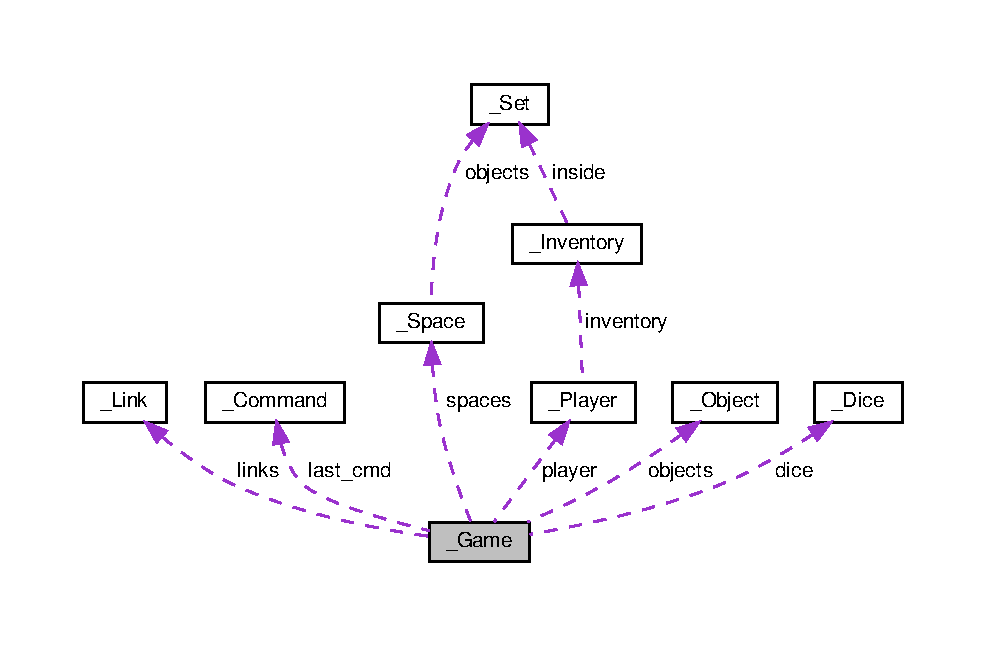
\includegraphics[width=350pt]{struct__Game__coll__graph}
\end{center}
\end{figure}
\subsection*{Data Fields}
\begin{DoxyCompactItemize}
\item 
\hyperlink{player_8h_af30e2030635a69690f85e48bc6ef202f}{Player} $\ast$ \hyperlink{struct__Game_a31406605782d71ec00c4bf258ea76267}{player}
\item 
\hyperlink{object_8h_a7f8bbcda919b65ce67f92fba08e0212f}{Object} $\ast$ \hyperlink{struct__Game_aa669bb857944c6c3b53504d179640af0}{objects} \mbox{[}\hyperlink{game_8h_acdc7844fbd4d45737d4aa56834d37829}{M\+A\+X\+\_\+\+O\+B\+J\+E\+C\+TS}+1\mbox{]}
\item 
\hyperlink{space_8h_a67533ffc2b70463baecc38fb0629bbfc}{Space} $\ast$ \hyperlink{struct__Game_ab4180417d9148f8abb2233ca6c4ecfe5}{spaces} \mbox{[}\hyperlink{space_8h_a5f54fd55f983a2e33ce076cd9f587e82}{M\+A\+X\+\_\+\+S\+P\+A\+C\+ES}+1\mbox{]}
\item 
\hyperlink{link_8h_ae3b299941e67be6971bfd64a25505eff}{Link} $\ast$ \hyperlink{struct__Game_a672f97aff892c65a6fdb43665cb57c97}{links} \mbox{[}\hyperlink{link_8h_a660ed1ec8604982002a0d6eced0e0367}{M\+A\+X\+\_\+\+L\+I\+N\+KS}+1\mbox{]}
\item 
\hyperlink{command_8h_a7d2935971c252377cb0fc1c8545dc2bc}{Command} $\ast$ \hyperlink{struct__Game_a47afef4b632256566d81da0f50e7a380}{last\+\_\+cmd}
\item 
\hyperlink{dice_8h_a5910ae86cf402855269700abd23e3976}{Dice} $\ast$ \hyperlink{struct__Game_af7004361a877182511a3e501b0949220}{dice}
\item 
\hyperlink{cmdAnswer_8h_a2e704274c270f99c8eaf383d11982d03}{Cmd\+Answer} $\ast$ \hyperlink{struct__Game_a4a34733add6a619004edb7326a8c300f}{Cmd\+Answer} \mbox{[}\hyperlink{game_8c_a8366e5ad74afbbea0cd0a414770c304a}{N\+\_\+\+C\+A\+L\+L\+B\+A\+CK}+1\mbox{]}
\item 
\hyperlink{npc_8h_a9529f25eaef52ee65aa84d4df6bb2d49}{Npc} $\ast$ \hyperlink{struct__Game_a41e78cf09a2a3fc90d9f27c99bdf9d3c}{npc} \mbox{[}\hyperlink{game_8c_a77f90fdf4bfbf2b0b6b5aded5458328d}{M\+A\+X\+\_\+\+N\+PC}+1\mbox{]}
\item 
char \hyperlink{struct__Game_a515c9531e4c918cd117ac503cf513076}{tutorial} \mbox{[}\hyperlink{types_8h_a92ed8507d1cd2331ad09275c5c4c1c89}{W\+O\+R\+D\+\_\+\+S\+I\+ZE}\mbox{]}
\item 
char \hyperlink{struct__Game_a712217e97c6ca0b8907fe40e4dc066c7}{End} \mbox{[}\hyperlink{types_8h_a92ed8507d1cd2331ad09275c5c4c1c89}{W\+O\+R\+D\+\_\+\+S\+I\+ZE}\mbox{]}
\end{DoxyCompactItemize}


\subsection{Detailed Description}
The game structure. 

It stores information of a game 

\subsection{Field Documentation}
\mbox{\Hypertarget{struct__Game_a4a34733add6a619004edb7326a8c300f}\label{struct__Game_a4a34733add6a619004edb7326a8c300f}} 
\index{\+\_\+\+Game@{\+\_\+\+Game}!Cmd\+Answer@{Cmd\+Answer}}
\index{Cmd\+Answer@{Cmd\+Answer}!\+\_\+\+Game@{\+\_\+\+Game}}
\subsubsection{\texorpdfstring{Cmd\+Answer}{CmdAnswer}}
{\footnotesize\ttfamily \hyperlink{cmdAnswer_8h_a2e704274c270f99c8eaf383d11982d03}{Cmd\+Answer}$\ast$ \+\_\+\+Game\+::\+Cmd\+Answer\mbox{[}\hyperlink{game_8c_a8366e5ad74afbbea0cd0a414770c304a}{N\+\_\+\+C\+A\+L\+L\+B\+A\+CK}+1\mbox{]}}

arraay of cmd\+Answer \mbox{\Hypertarget{struct__Game_af7004361a877182511a3e501b0949220}\label{struct__Game_af7004361a877182511a3e501b0949220}} 
\index{\+\_\+\+Game@{\+\_\+\+Game}!dice@{dice}}
\index{dice@{dice}!\+\_\+\+Game@{\+\_\+\+Game}}
\subsubsection{\texorpdfstring{dice}{dice}}
{\footnotesize\ttfamily \hyperlink{dice_8h_a5910ae86cf402855269700abd23e3976}{Dice}$\ast$ \+\_\+\+Game\+::dice}

dice of the game \mbox{\Hypertarget{struct__Game_a712217e97c6ca0b8907fe40e4dc066c7}\label{struct__Game_a712217e97c6ca0b8907fe40e4dc066c7}} 
\index{\+\_\+\+Game@{\+\_\+\+Game}!End@{End}}
\index{End@{End}!\+\_\+\+Game@{\+\_\+\+Game}}
\subsubsection{\texorpdfstring{End}{End}}
{\footnotesize\ttfamily char \+\_\+\+Game\+::\+End\mbox{[}\hyperlink{types_8h_a92ed8507d1cd2331ad09275c5c4c1c89}{W\+O\+R\+D\+\_\+\+S\+I\+ZE}\mbox{]}}

string with the end of the game \mbox{\Hypertarget{struct__Game_a47afef4b632256566d81da0f50e7a380}\label{struct__Game_a47afef4b632256566d81da0f50e7a380}} 
\index{\+\_\+\+Game@{\+\_\+\+Game}!last\+\_\+cmd@{last\+\_\+cmd}}
\index{last\+\_\+cmd@{last\+\_\+cmd}!\+\_\+\+Game@{\+\_\+\+Game}}
\subsubsection{\texorpdfstring{last\+\_\+cmd}{last\_cmd}}
{\footnotesize\ttfamily \hyperlink{command_8h_a7d2935971c252377cb0fc1c8545dc2bc}{Command}$\ast$ \+\_\+\+Game\+::last\+\_\+cmd}

last command written by the user \mbox{\Hypertarget{struct__Game_a672f97aff892c65a6fdb43665cb57c97}\label{struct__Game_a672f97aff892c65a6fdb43665cb57c97}} 
\index{\+\_\+\+Game@{\+\_\+\+Game}!links@{links}}
\index{links@{links}!\+\_\+\+Game@{\+\_\+\+Game}}
\subsubsection{\texorpdfstring{links}{links}}
{\footnotesize\ttfamily \hyperlink{link_8h_ae3b299941e67be6971bfd64a25505eff}{Link}$\ast$ \+\_\+\+Game\+::links\mbox{[}\hyperlink{link_8h_a660ed1ec8604982002a0d6eced0e0367}{M\+A\+X\+\_\+\+L\+I\+N\+KS}+1\mbox{]}}

links of the game \mbox{\Hypertarget{struct__Game_a41e78cf09a2a3fc90d9f27c99bdf9d3c}\label{struct__Game_a41e78cf09a2a3fc90d9f27c99bdf9d3c}} 
\index{\+\_\+\+Game@{\+\_\+\+Game}!npc@{npc}}
\index{npc@{npc}!\+\_\+\+Game@{\+\_\+\+Game}}
\subsubsection{\texorpdfstring{npc}{npc}}
{\footnotesize\ttfamily \hyperlink{npc_8h_a9529f25eaef52ee65aa84d4df6bb2d49}{Npc}$\ast$ \+\_\+\+Game\+::npc\mbox{[}\hyperlink{game_8c_a77f90fdf4bfbf2b0b6b5aded5458328d}{M\+A\+X\+\_\+\+N\+PC}+1\mbox{]}}

the npc of the game \mbox{\Hypertarget{struct__Game_aa669bb857944c6c3b53504d179640af0}\label{struct__Game_aa669bb857944c6c3b53504d179640af0}} 
\index{\+\_\+\+Game@{\+\_\+\+Game}!objects@{objects}}
\index{objects@{objects}!\+\_\+\+Game@{\+\_\+\+Game}}
\subsubsection{\texorpdfstring{objects}{objects}}
{\footnotesize\ttfamily \hyperlink{object_8h_a7f8bbcda919b65ce67f92fba08e0212f}{Object}$\ast$ \+\_\+\+Game\+::objects\mbox{[}\hyperlink{game_8h_acdc7844fbd4d45737d4aa56834d37829}{M\+A\+X\+\_\+\+O\+B\+J\+E\+C\+TS}+1\mbox{]}}

object of the game \mbox{\Hypertarget{struct__Game_a31406605782d71ec00c4bf258ea76267}\label{struct__Game_a31406605782d71ec00c4bf258ea76267}} 
\index{\+\_\+\+Game@{\+\_\+\+Game}!player@{player}}
\index{player@{player}!\+\_\+\+Game@{\+\_\+\+Game}}
\subsubsection{\texorpdfstring{player}{player}}
{\footnotesize\ttfamily \hyperlink{player_8h_af30e2030635a69690f85e48bc6ef202f}{Player}$\ast$ \+\_\+\+Game\+::player}

player of the game \mbox{\Hypertarget{struct__Game_ab4180417d9148f8abb2233ca6c4ecfe5}\label{struct__Game_ab4180417d9148f8abb2233ca6c4ecfe5}} 
\index{\+\_\+\+Game@{\+\_\+\+Game}!spaces@{spaces}}
\index{spaces@{spaces}!\+\_\+\+Game@{\+\_\+\+Game}}
\subsubsection{\texorpdfstring{spaces}{spaces}}
{\footnotesize\ttfamily \hyperlink{space_8h_a67533ffc2b70463baecc38fb0629bbfc}{Space}$\ast$ \+\_\+\+Game\+::spaces\mbox{[}\hyperlink{space_8h_a5f54fd55f983a2e33ce076cd9f587e82}{M\+A\+X\+\_\+\+S\+P\+A\+C\+ES}+1\mbox{]}}

spaces of the game \mbox{\Hypertarget{struct__Game_a515c9531e4c918cd117ac503cf513076}\label{struct__Game_a515c9531e4c918cd117ac503cf513076}} 
\index{\+\_\+\+Game@{\+\_\+\+Game}!tutorial@{tutorial}}
\index{tutorial@{tutorial}!\+\_\+\+Game@{\+\_\+\+Game}}
\subsubsection{\texorpdfstring{tutorial}{tutorial}}
{\footnotesize\ttfamily char \+\_\+\+Game\+::tutorial\mbox{[}\hyperlink{types_8h_a92ed8507d1cd2331ad09275c5c4c1c89}{W\+O\+R\+D\+\_\+\+S\+I\+ZE}\mbox{]}}

string with the tutorial/introduction of the game 

The documentation for this struct was generated from the following file\+:\begin{DoxyCompactItemize}
\item 
src/\hyperlink{game_8c}{game.\+c}\end{DoxyCompactItemize}

\hypertarget{struct__Graphic__engine}{}\section{\+\_\+\+Graphic\+\_\+engine Struct Reference}
\label{struct__Graphic__engine}\index{\+\_\+\+Graphic\+\_\+engine@{\+\_\+\+Graphic\+\_\+engine}}


The graic engine structure.  




Collaboration diagram for \+\_\+\+Graphic\+\_\+engine\+:\nopagebreak
\begin{figure}[H]
\begin{center}
\leavevmode
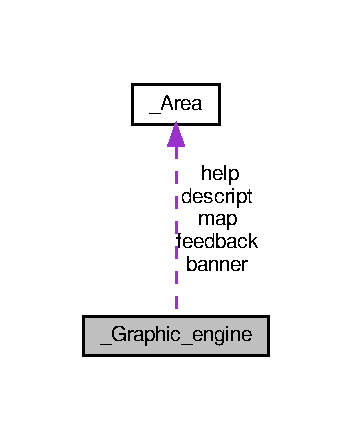
\includegraphics[width=169pt]{struct__Graphic__engine__coll__graph}
\end{center}
\end{figure}
\subsection*{Data Fields}
\begin{DoxyCompactItemize}
\item 
\hyperlink{screen_8h_acfdfc42f6522d75fa3c16713afde8127}{Area} $\ast$ \hyperlink{struct__Graphic__engine_a1ea06bb881d335da8c31d63b3e834bdb}{map}
\item 
\hyperlink{screen_8h_acfdfc42f6522d75fa3c16713afde8127}{Area} $\ast$ \hyperlink{struct__Graphic__engine_a414bb888ecce3389c7ce348264758e58}{descript}
\item 
\hyperlink{screen_8h_acfdfc42f6522d75fa3c16713afde8127}{Area} $\ast$ \hyperlink{struct__Graphic__engine_a440dfb2c23c3c4b7d3871187371117b9}{banner}
\item 
\hyperlink{screen_8h_acfdfc42f6522d75fa3c16713afde8127}{Area} $\ast$ \hyperlink{struct__Graphic__engine_ade1d3e95ad6def427f613a4a2d101875}{help}
\item 
\hyperlink{screen_8h_acfdfc42f6522d75fa3c16713afde8127}{Area} $\ast$ \hyperlink{struct__Graphic__engine_a4fc0ef353d000b20d57fb75d898c6d2d}{feedback}
\item 
\hyperlink{screen_8h_acfdfc42f6522d75fa3c16713afde8127}{Area} $\ast$ \hyperlink{struct__Graphic__engine_a9aefefc40ce56ccf7dd9639a53cd5463}{chat}
\end{DoxyCompactItemize}


\subsection{Detailed Description}
The graic engine structure. 

It stores information of the graphic engine 

\subsection{Field Documentation}
\mbox{\Hypertarget{struct__Graphic__engine_a440dfb2c23c3c4b7d3871187371117b9}\label{struct__Graphic__engine_a440dfb2c23c3c4b7d3871187371117b9}} 
\index{\+\_\+\+Graphic\+\_\+engine@{\+\_\+\+Graphic\+\_\+engine}!banner@{banner}}
\index{banner@{banner}!\+\_\+\+Graphic\+\_\+engine@{\+\_\+\+Graphic\+\_\+engine}}
\subsubsection{\texorpdfstring{banner}{banner}}
{\footnotesize\ttfamily \hyperlink{screen_8h_acfdfc42f6522d75fa3c16713afde8127}{Area}$\ast$ \+\_\+\+Graphic\+\_\+engine\+::banner}

Area of banner \mbox{\Hypertarget{struct__Graphic__engine_a9aefefc40ce56ccf7dd9639a53cd5463}\label{struct__Graphic__engine_a9aefefc40ce56ccf7dd9639a53cd5463}} 
\index{\+\_\+\+Graphic\+\_\+engine@{\+\_\+\+Graphic\+\_\+engine}!chat@{chat}}
\index{chat@{chat}!\+\_\+\+Graphic\+\_\+engine@{\+\_\+\+Graphic\+\_\+engine}}
\subsubsection{\texorpdfstring{chat}{chat}}
{\footnotesize\ttfamily \hyperlink{screen_8h_acfdfc42f6522d75fa3c16713afde8127}{Area}$\ast$ \+\_\+\+Graphic\+\_\+engine\+::chat}

Area of chat \mbox{\Hypertarget{struct__Graphic__engine_a414bb888ecce3389c7ce348264758e58}\label{struct__Graphic__engine_a414bb888ecce3389c7ce348264758e58}} 
\index{\+\_\+\+Graphic\+\_\+engine@{\+\_\+\+Graphic\+\_\+engine}!descript@{descript}}
\index{descript@{descript}!\+\_\+\+Graphic\+\_\+engine@{\+\_\+\+Graphic\+\_\+engine}}
\subsubsection{\texorpdfstring{descript}{descript}}
{\footnotesize\ttfamily \hyperlink{screen_8h_acfdfc42f6522d75fa3c16713afde8127}{Area}$\ast$ \+\_\+\+Graphic\+\_\+engine\+::descript}

Area of descript \mbox{\Hypertarget{struct__Graphic__engine_a4fc0ef353d000b20d57fb75d898c6d2d}\label{struct__Graphic__engine_a4fc0ef353d000b20d57fb75d898c6d2d}} 
\index{\+\_\+\+Graphic\+\_\+engine@{\+\_\+\+Graphic\+\_\+engine}!feedback@{feedback}}
\index{feedback@{feedback}!\+\_\+\+Graphic\+\_\+engine@{\+\_\+\+Graphic\+\_\+engine}}
\subsubsection{\texorpdfstring{feedback}{feedback}}
{\footnotesize\ttfamily \hyperlink{screen_8h_acfdfc42f6522d75fa3c16713afde8127}{Area}$\ast$ \+\_\+\+Graphic\+\_\+engine\+::feedback}

Area of feedback \mbox{\Hypertarget{struct__Graphic__engine_ade1d3e95ad6def427f613a4a2d101875}\label{struct__Graphic__engine_ade1d3e95ad6def427f613a4a2d101875}} 
\index{\+\_\+\+Graphic\+\_\+engine@{\+\_\+\+Graphic\+\_\+engine}!help@{help}}
\index{help@{help}!\+\_\+\+Graphic\+\_\+engine@{\+\_\+\+Graphic\+\_\+engine}}
\subsubsection{\texorpdfstring{help}{help}}
{\footnotesize\ttfamily \hyperlink{screen_8h_acfdfc42f6522d75fa3c16713afde8127}{Area}$\ast$ \+\_\+\+Graphic\+\_\+engine\+::help}

Area of help \mbox{\Hypertarget{struct__Graphic__engine_a1ea06bb881d335da8c31d63b3e834bdb}\label{struct__Graphic__engine_a1ea06bb881d335da8c31d63b3e834bdb}} 
\index{\+\_\+\+Graphic\+\_\+engine@{\+\_\+\+Graphic\+\_\+engine}!map@{map}}
\index{map@{map}!\+\_\+\+Graphic\+\_\+engine@{\+\_\+\+Graphic\+\_\+engine}}
\subsubsection{\texorpdfstring{map}{map}}
{\footnotesize\ttfamily \hyperlink{screen_8h_acfdfc42f6522d75fa3c16713afde8127}{Area}$\ast$ \+\_\+\+Graphic\+\_\+engine\+::map}

Area of map 

The documentation for this struct was generated from the following file\+:\begin{DoxyCompactItemize}
\item 
src/graphic\+\_\+engine.\+c\end{DoxyCompactItemize}

\hypertarget{struct__Inventory}{}\section{\+\_\+\+Inventory Struct Reference}
\label{struct__Inventory}\index{\+\_\+\+Inventory@{\+\_\+\+Inventory}}


The inventory structure.  




Collaboration diagram for \+\_\+\+Inventory\+:\nopagebreak
\begin{figure}[H]
\begin{center}
\leavevmode
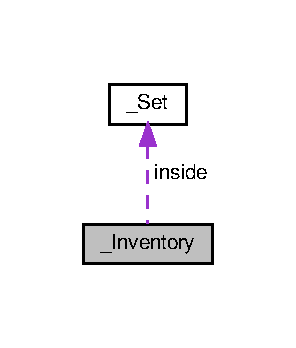
\includegraphics[width=142pt]{struct__Inventory__coll__graph}
\end{center}
\end{figure}
\subsection*{Data Fields}
\begin{DoxyCompactItemize}
\item 
\hyperlink{types_8h_a845e604fb28f7e3d97549da3448149d3}{Id} \hyperlink{struct__Inventory_a73dcd4e1c702c8234092eac3ca2753f6}{id}
\item 
\hyperlink{set_8h_a6d3b7f7c92cbb4577ef3ef7ddbf93161}{Set} $\ast$ \hyperlink{struct__Inventory_ab6ad3d65f6119379be87edf22db640cb}{inside}
\item 
int \hyperlink{struct__Inventory_ac09bcf212b2c7ff348066b2e5f28bb9c}{max}
\end{DoxyCompactItemize}


\subsection{Detailed Description}
The inventory structure. 

It stores information of a inventory 

\subsection{Field Documentation}
\mbox{\Hypertarget{struct__Inventory_a73dcd4e1c702c8234092eac3ca2753f6}\label{struct__Inventory_a73dcd4e1c702c8234092eac3ca2753f6}} 
\index{\+\_\+\+Inventory@{\+\_\+\+Inventory}!id@{id}}
\index{id@{id}!\+\_\+\+Inventory@{\+\_\+\+Inventory}}
\subsubsection{\texorpdfstring{id}{id}}
{\footnotesize\ttfamily \hyperlink{types_8h_a845e604fb28f7e3d97549da3448149d3}{Id} \+\_\+\+Inventory\+::id}

the id of an inventory \mbox{\Hypertarget{struct__Inventory_ab6ad3d65f6119379be87edf22db640cb}\label{struct__Inventory_ab6ad3d65f6119379be87edf22db640cb}} 
\index{\+\_\+\+Inventory@{\+\_\+\+Inventory}!inside@{inside}}
\index{inside@{inside}!\+\_\+\+Inventory@{\+\_\+\+Inventory}}
\subsubsection{\texorpdfstring{inside}{inside}}
{\footnotesize\ttfamily \hyperlink{set_8h_a6d3b7f7c92cbb4577ef3ef7ddbf93161}{Set}$\ast$ \+\_\+\+Inventory\+::inside}

the set inside the inventory \mbox{\Hypertarget{struct__Inventory_ac09bcf212b2c7ff348066b2e5f28bb9c}\label{struct__Inventory_ac09bcf212b2c7ff348066b2e5f28bb9c}} 
\index{\+\_\+\+Inventory@{\+\_\+\+Inventory}!max@{max}}
\index{max@{max}!\+\_\+\+Inventory@{\+\_\+\+Inventory}}
\subsubsection{\texorpdfstring{max}{max}}
{\footnotesize\ttfamily int \+\_\+\+Inventory\+::max}

the max objetcs that can be stored in the inventory 

The documentation for this struct was generated from the following file\+:\begin{DoxyCompactItemize}
\item 
/home/dgr/\+Escritorio/universidad/pprog/iteraciones\+\_\+corregidas/\+I3-\/seguro\+\_\+v21.\+0/src/\hyperlink{inventory_8c}{inventory.\+c}\end{DoxyCompactItemize}

\hypertarget{struct__Link}{}\section{\+\_\+\+Link Struct Reference}
\label{struct__Link}\index{\+\_\+\+Link@{\+\_\+\+Link}}


The link structure.  


\subsection*{Data Fields}
\begin{DoxyCompactItemize}
\item 
char \hyperlink{struct__Link_a020ee863120055b29609157b9de3c84d}{name} \mbox{[}\hyperlink{types_8h_a92ed8507d1cd2331ad09275c5c4c1c89}{W\+O\+R\+D\+\_\+\+S\+I\+ZE}+1\mbox{]}
\item 
\hyperlink{types_8h_a845e604fb28f7e3d97549da3448149d3}{Id} \hyperlink{struct__Link_a151212e7a8e8274c2a1ee991ba95878b}{id}
\item 
\hyperlink{types_8h_a845e604fb28f7e3d97549da3448149d3}{Id} \hyperlink{struct__Link_a62d6aee205ac5d4d738bb7448fbaf9cc}{id1}
\item 
\hyperlink{types_8h_a845e604fb28f7e3d97549da3448149d3}{Id} \hyperlink{struct__Link_a9d8710f0f005598c8d6a1b48d5bf07d7}{id2}
\item 
int \hyperlink{struct__Link_a5df9107f4ea513f3741d9e4883f4678a}{open}
\end{DoxyCompactItemize}


\subsection{Detailed Description}
The link structure. 

It stores information of a link 

\subsection{Field Documentation}
\mbox{\Hypertarget{struct__Link_a151212e7a8e8274c2a1ee991ba95878b}\label{struct__Link_a151212e7a8e8274c2a1ee991ba95878b}} 
\index{\+\_\+\+Link@{\+\_\+\+Link}!id@{id}}
\index{id@{id}!\+\_\+\+Link@{\+\_\+\+Link}}
\subsubsection{\texorpdfstring{id}{id}}
{\footnotesize\ttfamily \hyperlink{types_8h_a845e604fb28f7e3d97549da3448149d3}{Id} \+\_\+\+Link\+::id}

the id of the link \mbox{\Hypertarget{struct__Link_a62d6aee205ac5d4d738bb7448fbaf9cc}\label{struct__Link_a62d6aee205ac5d4d738bb7448fbaf9cc}} 
\index{\+\_\+\+Link@{\+\_\+\+Link}!id1@{id1}}
\index{id1@{id1}!\+\_\+\+Link@{\+\_\+\+Link}}
\subsubsection{\texorpdfstring{id1}{id1}}
{\footnotesize\ttfamily \hyperlink{types_8h_a845e604fb28f7e3d97549da3448149d3}{Id} \+\_\+\+Link\+::id1}

the id of the first link \mbox{\Hypertarget{struct__Link_a9d8710f0f005598c8d6a1b48d5bf07d7}\label{struct__Link_a9d8710f0f005598c8d6a1b48d5bf07d7}} 
\index{\+\_\+\+Link@{\+\_\+\+Link}!id2@{id2}}
\index{id2@{id2}!\+\_\+\+Link@{\+\_\+\+Link}}
\subsubsection{\texorpdfstring{id2}{id2}}
{\footnotesize\ttfamily \hyperlink{types_8h_a845e604fb28f7e3d97549da3448149d3}{Id} \+\_\+\+Link\+::id2}

the id of the secod link \mbox{\Hypertarget{struct__Link_a020ee863120055b29609157b9de3c84d}\label{struct__Link_a020ee863120055b29609157b9de3c84d}} 
\index{\+\_\+\+Link@{\+\_\+\+Link}!name@{name}}
\index{name@{name}!\+\_\+\+Link@{\+\_\+\+Link}}
\subsubsection{\texorpdfstring{name}{name}}
{\footnotesize\ttfamily char \+\_\+\+Link\+::name\mbox{[}\hyperlink{types_8h_a92ed8507d1cd2331ad09275c5c4c1c89}{W\+O\+R\+D\+\_\+\+S\+I\+ZE}+1\mbox{]}}

the name of the link \mbox{\Hypertarget{struct__Link_a5df9107f4ea513f3741d9e4883f4678a}\label{struct__Link_a5df9107f4ea513f3741d9e4883f4678a}} 
\index{\+\_\+\+Link@{\+\_\+\+Link}!open@{open}}
\index{open@{open}!\+\_\+\+Link@{\+\_\+\+Link}}
\subsubsection{\texorpdfstring{open}{open}}
{\footnotesize\ttfamily int \+\_\+\+Link\+::open}

an integer to determine whether or not a link is open 

The documentation for this struct was generated from the following file\+:\begin{DoxyCompactItemize}
\item 
/home/dgr/\+Escritorio/universidad/pprog/iteraciones\+\_\+corregidas/\+I3-\/seguro\+\_\+v21.\+0/src/\hyperlink{link_8c}{link.\+c}\end{DoxyCompactItemize}

\hypertarget{struct__Object}{}\section{\+\_\+\+Object Struct Reference}
\label{struct__Object}\index{\+\_\+\+Object@{\+\_\+\+Object}}


The object structure.  


\subsection*{Data Fields}
\begin{DoxyCompactItemize}
\item 
\hyperlink{types_8h_a845e604fb28f7e3d97549da3448149d3}{Id} \hyperlink{struct__Object_a3cff7a0e8dc4e9d23895ed9af1b7653a}{id}
\item 
char \hyperlink{struct__Object_a3dab853826b88558a2c07dec50b96d57}{name} \mbox{[}\hyperlink{types_8h_a92ed8507d1cd2331ad09275c5c4c1c89}{W\+O\+R\+D\+\_\+\+S\+I\+ZE}\mbox{]}
\item 
char \hyperlink{struct__Object_a556e2e37c1461bcaae6492d2101f407d}{description} \mbox{[}\hyperlink{types_8h_a92ed8507d1cd2331ad09275c5c4c1c89}{W\+O\+R\+D\+\_\+\+S\+I\+ZE}\mbox{]}
\end{DoxyCompactItemize}


\subsection{Detailed Description}
The object structure. 

It stores information of an object 

\subsection{Field Documentation}
\mbox{\Hypertarget{struct__Object_a556e2e37c1461bcaae6492d2101f407d}\label{struct__Object_a556e2e37c1461bcaae6492d2101f407d}} 
\index{\+\_\+\+Object@{\+\_\+\+Object}!description@{description}}
\index{description@{description}!\+\_\+\+Object@{\+\_\+\+Object}}
\subsubsection{\texorpdfstring{description}{description}}
{\footnotesize\ttfamily char \+\_\+\+Object\+::description\mbox{[}\hyperlink{types_8h_a92ed8507d1cd2331ad09275c5c4c1c89}{W\+O\+R\+D\+\_\+\+S\+I\+ZE}\mbox{]}}

description of the object \mbox{\Hypertarget{struct__Object_a3cff7a0e8dc4e9d23895ed9af1b7653a}\label{struct__Object_a3cff7a0e8dc4e9d23895ed9af1b7653a}} 
\index{\+\_\+\+Object@{\+\_\+\+Object}!id@{id}}
\index{id@{id}!\+\_\+\+Object@{\+\_\+\+Object}}
\subsubsection{\texorpdfstring{id}{id}}
{\footnotesize\ttfamily \hyperlink{types_8h_a845e604fb28f7e3d97549da3448149d3}{Id} \+\_\+\+Object\+::id}

object identifier \mbox{\Hypertarget{struct__Object_a3dab853826b88558a2c07dec50b96d57}\label{struct__Object_a3dab853826b88558a2c07dec50b96d57}} 
\index{\+\_\+\+Object@{\+\_\+\+Object}!name@{name}}
\index{name@{name}!\+\_\+\+Object@{\+\_\+\+Object}}
\subsubsection{\texorpdfstring{name}{name}}
{\footnotesize\ttfamily char \+\_\+\+Object\+::name\mbox{[}\hyperlink{types_8h_a92ed8507d1cd2331ad09275c5c4c1c89}{W\+O\+R\+D\+\_\+\+S\+I\+ZE}\mbox{]}}

object name 

The documentation for this struct was generated from the following file\+:\begin{DoxyCompactItemize}
\item 
/home/dgr/\+Escritorio/universidad/pprog/iteraciones\+\_\+corregidas/\+I3-\/seguro\+\_\+v21.\+0/src/\hyperlink{object_8c}{object.\+c}\end{DoxyCompactItemize}

\hypertarget{struct__Player}{}\section{\+\_\+\+Player Struct Reference}
\label{struct__Player}\index{\+\_\+\+Player@{\+\_\+\+Player}}


The oplayer structure.  




Collaboration diagram for \+\_\+\+Player\+:\nopagebreak
\begin{figure}[H]
\begin{center}
\leavevmode
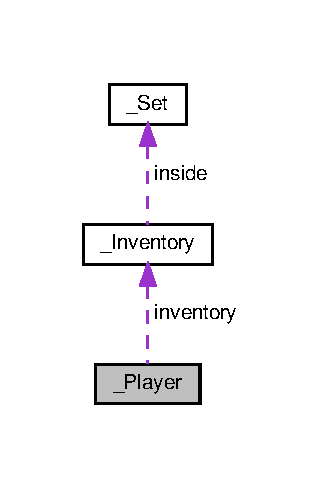
\includegraphics[width=154pt]{struct__Player__coll__graph}
\end{center}
\end{figure}
\subsection*{Data Fields}
\begin{DoxyCompactItemize}
\item 
\hyperlink{types_8h_a845e604fb28f7e3d97549da3448149d3}{Id} \hyperlink{struct__Player_a60d635cd063816a9c1bd873f4868bb90}{id}
\item 
char \hyperlink{struct__Player_adda99df91c28eb58d392f2b43fc6898f}{name} \mbox{[}\hyperlink{types_8h_a92ed8507d1cd2331ad09275c5c4c1c89}{W\+O\+R\+D\+\_\+\+S\+I\+ZE}\mbox{]}
\item 
\hyperlink{types_8h_a845e604fb28f7e3d97549da3448149d3}{Id} \hyperlink{struct__Player_adbb6195d15b88f3f658e74274eff52d8}{location}
\item 
\hyperlink{inventory_8h_a2253bf64ac4ce6a9c1d6f39c0b0d32a3}{Inventory} $\ast$ \hyperlink{struct__Player_a5e02924cb82ca61f74ba414d190aa29b}{inventory}
\end{DoxyCompactItemize}


\subsection{Detailed Description}
The oplayer structure. 

It stores information of the different players managed by the sytem 

\subsection{Field Documentation}
\mbox{\Hypertarget{struct__Player_a60d635cd063816a9c1bd873f4868bb90}\label{struct__Player_a60d635cd063816a9c1bd873f4868bb90}} 
\index{\+\_\+\+Player@{\+\_\+\+Player}!id@{id}}
\index{id@{id}!\+\_\+\+Player@{\+\_\+\+Player}}
\subsubsection{\texorpdfstring{id}{id}}
{\footnotesize\ttfamily \hyperlink{types_8h_a845e604fb28f7e3d97549da3448149d3}{Id} \+\_\+\+Player\+::id}

Id of the player \mbox{\Hypertarget{struct__Player_a5e02924cb82ca61f74ba414d190aa29b}\label{struct__Player_a5e02924cb82ca61f74ba414d190aa29b}} 
\index{\+\_\+\+Player@{\+\_\+\+Player}!inventory@{inventory}}
\index{inventory@{inventory}!\+\_\+\+Player@{\+\_\+\+Player}}
\subsubsection{\texorpdfstring{inventory}{inventory}}
{\footnotesize\ttfamily \hyperlink{inventory_8h_a2253bf64ac4ce6a9c1d6f39c0b0d32a3}{Inventory}$\ast$ \+\_\+\+Player\+::inventory}

objects in possesion of the player \mbox{\Hypertarget{struct__Player_adbb6195d15b88f3f658e74274eff52d8}\label{struct__Player_adbb6195d15b88f3f658e74274eff52d8}} 
\index{\+\_\+\+Player@{\+\_\+\+Player}!location@{location}}
\index{location@{location}!\+\_\+\+Player@{\+\_\+\+Player}}
\subsubsection{\texorpdfstring{location}{location}}
{\footnotesize\ttfamily \hyperlink{types_8h_a845e604fb28f7e3d97549da3448149d3}{Id} \+\_\+\+Player\+::location}

location of the player \mbox{\Hypertarget{struct__Player_adda99df91c28eb58d392f2b43fc6898f}\label{struct__Player_adda99df91c28eb58d392f2b43fc6898f}} 
\index{\+\_\+\+Player@{\+\_\+\+Player}!name@{name}}
\index{name@{name}!\+\_\+\+Player@{\+\_\+\+Player}}
\subsubsection{\texorpdfstring{name}{name}}
{\footnotesize\ttfamily char \+\_\+\+Player\+::name\mbox{[}\hyperlink{types_8h_a92ed8507d1cd2331ad09275c5c4c1c89}{W\+O\+R\+D\+\_\+\+S\+I\+ZE}\mbox{]}}

name of the player 

The documentation for this struct was generated from the following file\+:\begin{DoxyCompactItemize}
\item 
src/player.\+c\end{DoxyCompactItemize}

\hypertarget{struct__Set}{}\section{\+\_\+\+Set Struct Reference}
\label{struct__Set}\index{\+\_\+\+Set@{\+\_\+\+Set}}


The set structure.  


\subsection*{Data Fields}
\begin{DoxyCompactItemize}
\item 
\hyperlink{types_8h_a845e604fb28f7e3d97549da3448149d3}{Id} \hyperlink{struct__Set_a54767c55da685696938857775301eaf0}{tabla} \mbox{[}\hyperlink{set_8c_a1cdef4472847c938fc165b7d2737c4e4}{M\+A\+X\+\_\+\+ID}\mbox{]}
\item 
int \hyperlink{struct__Set_a0695075759bf06cffe79a8c3d8bfcfed}{num}
\end{DoxyCompactItemize}


\subsection{Detailed Description}
The set structure. 

It stores information of an object 

\subsection{Field Documentation}
\mbox{\Hypertarget{struct__Set_a0695075759bf06cffe79a8c3d8bfcfed}\label{struct__Set_a0695075759bf06cffe79a8c3d8bfcfed}} 
\index{\+\_\+\+Set@{\+\_\+\+Set}!num@{num}}
\index{num@{num}!\+\_\+\+Set@{\+\_\+\+Set}}
\subsubsection{\texorpdfstring{num}{num}}
{\footnotesize\ttfamily int \+\_\+\+Set\+::num}

number of identifiers \mbox{\Hypertarget{struct__Set_a54767c55da685696938857775301eaf0}\label{struct__Set_a54767c55da685696938857775301eaf0}} 
\index{\+\_\+\+Set@{\+\_\+\+Set}!tabla@{tabla}}
\index{tabla@{tabla}!\+\_\+\+Set@{\+\_\+\+Set}}
\subsubsection{\texorpdfstring{tabla}{tabla}}
{\footnotesize\ttfamily \hyperlink{types_8h_a845e604fb28f7e3d97549da3448149d3}{Id} \+\_\+\+Set\+::tabla\mbox{[}\hyperlink{set_8c_a1cdef4472847c938fc165b7d2737c4e4}{M\+A\+X\+\_\+\+ID}\mbox{]}}

array of identifiers 

The documentation for this struct was generated from the following file\+:\begin{DoxyCompactItemize}
\item 
/home/dgr/\+Escritorio/universidad/pprog/iteraciones\+\_\+corregidas/\+I3-\/seguro\+\_\+v21.\+0/src/\hyperlink{set_8c}{set.\+c}\end{DoxyCompactItemize}

\hypertarget{struct__Space}{}\section{\+\_\+\+Space Struct Reference}
\label{struct__Space}\index{\+\_\+\+Space@{\+\_\+\+Space}}


The space structure.  




Collaboration diagram for \+\_\+\+Space\+:\nopagebreak
\begin{figure}[H]
\begin{center}
\leavevmode
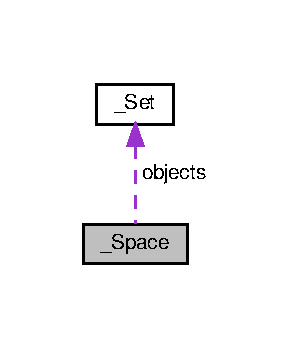
\includegraphics[width=140pt]{struct__Space__coll__graph}
\end{center}
\end{figure}
\subsection*{Data Fields}
\begin{DoxyCompactItemize}
\item 
\hyperlink{types_8h_a845e604fb28f7e3d97549da3448149d3}{Id} \hyperlink{struct__Space_a70cb461deb9ac073e401b607339b567f}{id}
\item 
char \hyperlink{struct__Space_aa1c9c994c2d16ecf3ef46138685fdfdc}{name} \mbox{[}\hyperlink{types_8h_a92ed8507d1cd2331ad09275c5c4c1c89}{W\+O\+R\+D\+\_\+\+S\+I\+ZE}+1\mbox{]}
\item 
\hyperlink{types_8h_a845e604fb28f7e3d97549da3448149d3}{Id} \hyperlink{struct__Space_ae5ebe53ce79514d7d2d93911e0159252}{north}
\item 
\hyperlink{types_8h_a845e604fb28f7e3d97549da3448149d3}{Id} \hyperlink{struct__Space_a646b68c22a0bbf1685033c96109d31d1}{south}
\item 
\hyperlink{types_8h_a845e604fb28f7e3d97549da3448149d3}{Id} \hyperlink{struct__Space_a41ce2bf33cf0c157b358221f094ee05b}{east}
\item 
\hyperlink{types_8h_a845e604fb28f7e3d97549da3448149d3}{Id} \hyperlink{struct__Space_a20c1d259e93b44e24ba82982e142eb9b}{west}
\item 
char \hyperlink{struct__Space_a0c4d07c615267b6d8744885709ad403d}{gdesc} \mbox{[}\hyperlink{space_8h_a9c6419e7f541d4daf14f5ccd56e03f17}{N\+U\+M\+\_\+\+S\+T\+R\+I\+N\+GS}\mbox{]}\mbox{[}\hyperlink{space_8h_a4f7414c5a72de21b6b45d462410dfc97}{N\+U\+M\+\_\+\+C\+H\+A\+R\+A\+C\+TS}\mbox{]}
\item 
\hyperlink{set_8h_a6d3b7f7c92cbb4577ef3ef7ddbf93161}{Set} $\ast$ \hyperlink{struct__Space_a661ed8b0fc8085b6db70188aa5085625}{objects}
\item 
char \hyperlink{struct__Space_a2a50aacb78d1d0f65f5b14f94ed81d80}{description} \mbox{[}\hyperlink{types_8h_a92ed8507d1cd2331ad09275c5c4c1c89}{W\+O\+R\+D\+\_\+\+S\+I\+ZE}\mbox{]}
\end{DoxyCompactItemize}


\subsection{Detailed Description}
The space structure. 

It stores information of the different spaces managed by the sytem 

\subsection{Field Documentation}
\mbox{\Hypertarget{struct__Space_a2a50aacb78d1d0f65f5b14f94ed81d80}\label{struct__Space_a2a50aacb78d1d0f65f5b14f94ed81d80}} 
\index{\+\_\+\+Space@{\+\_\+\+Space}!description@{description}}
\index{description@{description}!\+\_\+\+Space@{\+\_\+\+Space}}
\subsubsection{\texorpdfstring{description}{description}}
{\footnotesize\ttfamily char \+\_\+\+Space\+::description\mbox{[}\hyperlink{types_8h_a92ed8507d1cd2331ad09275c5c4c1c89}{W\+O\+R\+D\+\_\+\+S\+I\+ZE}\mbox{]}}

description of an space \mbox{\Hypertarget{struct__Space_a41ce2bf33cf0c157b358221f094ee05b}\label{struct__Space_a41ce2bf33cf0c157b358221f094ee05b}} 
\index{\+\_\+\+Space@{\+\_\+\+Space}!east@{east}}
\index{east@{east}!\+\_\+\+Space@{\+\_\+\+Space}}
\subsubsection{\texorpdfstring{east}{east}}
{\footnotesize\ttfamily \hyperlink{types_8h_a845e604fb28f7e3d97549da3448149d3}{Id} \+\_\+\+Space\+::east}

Id of the east link \mbox{\Hypertarget{struct__Space_a0c4d07c615267b6d8744885709ad403d}\label{struct__Space_a0c4d07c615267b6d8744885709ad403d}} 
\index{\+\_\+\+Space@{\+\_\+\+Space}!gdesc@{gdesc}}
\index{gdesc@{gdesc}!\+\_\+\+Space@{\+\_\+\+Space}}
\subsubsection{\texorpdfstring{gdesc}{gdesc}}
{\footnotesize\ttfamily char \+\_\+\+Space\+::gdesc\mbox{[}\hyperlink{space_8h_a9c6419e7f541d4daf14f5ccd56e03f17}{N\+U\+M\+\_\+\+S\+T\+R\+I\+N\+GS}\mbox{]}\mbox{[}\hyperlink{space_8h_a4f7414c5a72de21b6b45d462410dfc97}{N\+U\+M\+\_\+\+C\+H\+A\+R\+A\+C\+TS}\mbox{]}}

the string with thediferents drawings \mbox{\Hypertarget{struct__Space_a70cb461deb9ac073e401b607339b567f}\label{struct__Space_a70cb461deb9ac073e401b607339b567f}} 
\index{\+\_\+\+Space@{\+\_\+\+Space}!id@{id}}
\index{id@{id}!\+\_\+\+Space@{\+\_\+\+Space}}
\subsubsection{\texorpdfstring{id}{id}}
{\footnotesize\ttfamily \hyperlink{types_8h_a845e604fb28f7e3d97549da3448149d3}{Id} \+\_\+\+Space\+::id}

Id of the space \mbox{\Hypertarget{struct__Space_aa1c9c994c2d16ecf3ef46138685fdfdc}\label{struct__Space_aa1c9c994c2d16ecf3ef46138685fdfdc}} 
\index{\+\_\+\+Space@{\+\_\+\+Space}!name@{name}}
\index{name@{name}!\+\_\+\+Space@{\+\_\+\+Space}}
\subsubsection{\texorpdfstring{name}{name}}
{\footnotesize\ttfamily char \+\_\+\+Space\+::name\mbox{[}\hyperlink{types_8h_a92ed8507d1cd2331ad09275c5c4c1c89}{W\+O\+R\+D\+\_\+\+S\+I\+ZE}+1\mbox{]}}

Name of the space \mbox{\Hypertarget{struct__Space_ae5ebe53ce79514d7d2d93911e0159252}\label{struct__Space_ae5ebe53ce79514d7d2d93911e0159252}} 
\index{\+\_\+\+Space@{\+\_\+\+Space}!north@{north}}
\index{north@{north}!\+\_\+\+Space@{\+\_\+\+Space}}
\subsubsection{\texorpdfstring{north}{north}}
{\footnotesize\ttfamily \hyperlink{types_8h_a845e604fb28f7e3d97549da3448149d3}{Id} \+\_\+\+Space\+::north}

Id of the north link \mbox{\Hypertarget{struct__Space_a661ed8b0fc8085b6db70188aa5085625}\label{struct__Space_a661ed8b0fc8085b6db70188aa5085625}} 
\index{\+\_\+\+Space@{\+\_\+\+Space}!objects@{objects}}
\index{objects@{objects}!\+\_\+\+Space@{\+\_\+\+Space}}
\subsubsection{\texorpdfstring{objects}{objects}}
{\footnotesize\ttfamily \hyperlink{set_8h_a6d3b7f7c92cbb4577ef3ef7ddbf93161}{Set}$\ast$ \+\_\+\+Space\+::objects}

set of objects \mbox{\Hypertarget{struct__Space_a646b68c22a0bbf1685033c96109d31d1}\label{struct__Space_a646b68c22a0bbf1685033c96109d31d1}} 
\index{\+\_\+\+Space@{\+\_\+\+Space}!south@{south}}
\index{south@{south}!\+\_\+\+Space@{\+\_\+\+Space}}
\subsubsection{\texorpdfstring{south}{south}}
{\footnotesize\ttfamily \hyperlink{types_8h_a845e604fb28f7e3d97549da3448149d3}{Id} \+\_\+\+Space\+::south}

Id of the south link \mbox{\Hypertarget{struct__Space_a20c1d259e93b44e24ba82982e142eb9b}\label{struct__Space_a20c1d259e93b44e24ba82982e142eb9b}} 
\index{\+\_\+\+Space@{\+\_\+\+Space}!west@{west}}
\index{west@{west}!\+\_\+\+Space@{\+\_\+\+Space}}
\subsubsection{\texorpdfstring{west}{west}}
{\footnotesize\ttfamily \hyperlink{types_8h_a845e604fb28f7e3d97549da3448149d3}{Id} \+\_\+\+Space\+::west}

Id of the weast link 

The documentation for this struct was generated from the following file\+:\begin{DoxyCompactItemize}
\item 
/home/dgr/\+Escritorio/universidad/pprog/iteraciones\+\_\+corregidas/\+I3-\/seguro\+\_\+v21.\+0/src/space.\+c\end{DoxyCompactItemize}

\chapter{File Documentation}
\hypertarget{command_8h}{}\section{include/command.h File Reference}
\label{command_8h}\index{include/command.\+h@{include/command.\+h}}


It implements the command interpreter.  


{\ttfamily \#include \char`\"{}../include/types.\+h\char`\"{}}\newline
{\ttfamily \#include $<$stdio.\+h$>$}\newline
Include dependency graph for command.\+h\+:\nopagebreak
\begin{figure}[H]
\begin{center}
\leavevmode
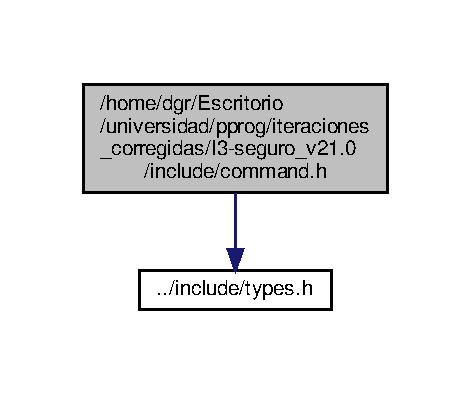
\includegraphics[width=236pt]{command_8h__incl}
\end{center}
\end{figure}
This graph shows which files directly or indirectly include this file\+:\nopagebreak
\begin{figure}[H]
\begin{center}
\leavevmode
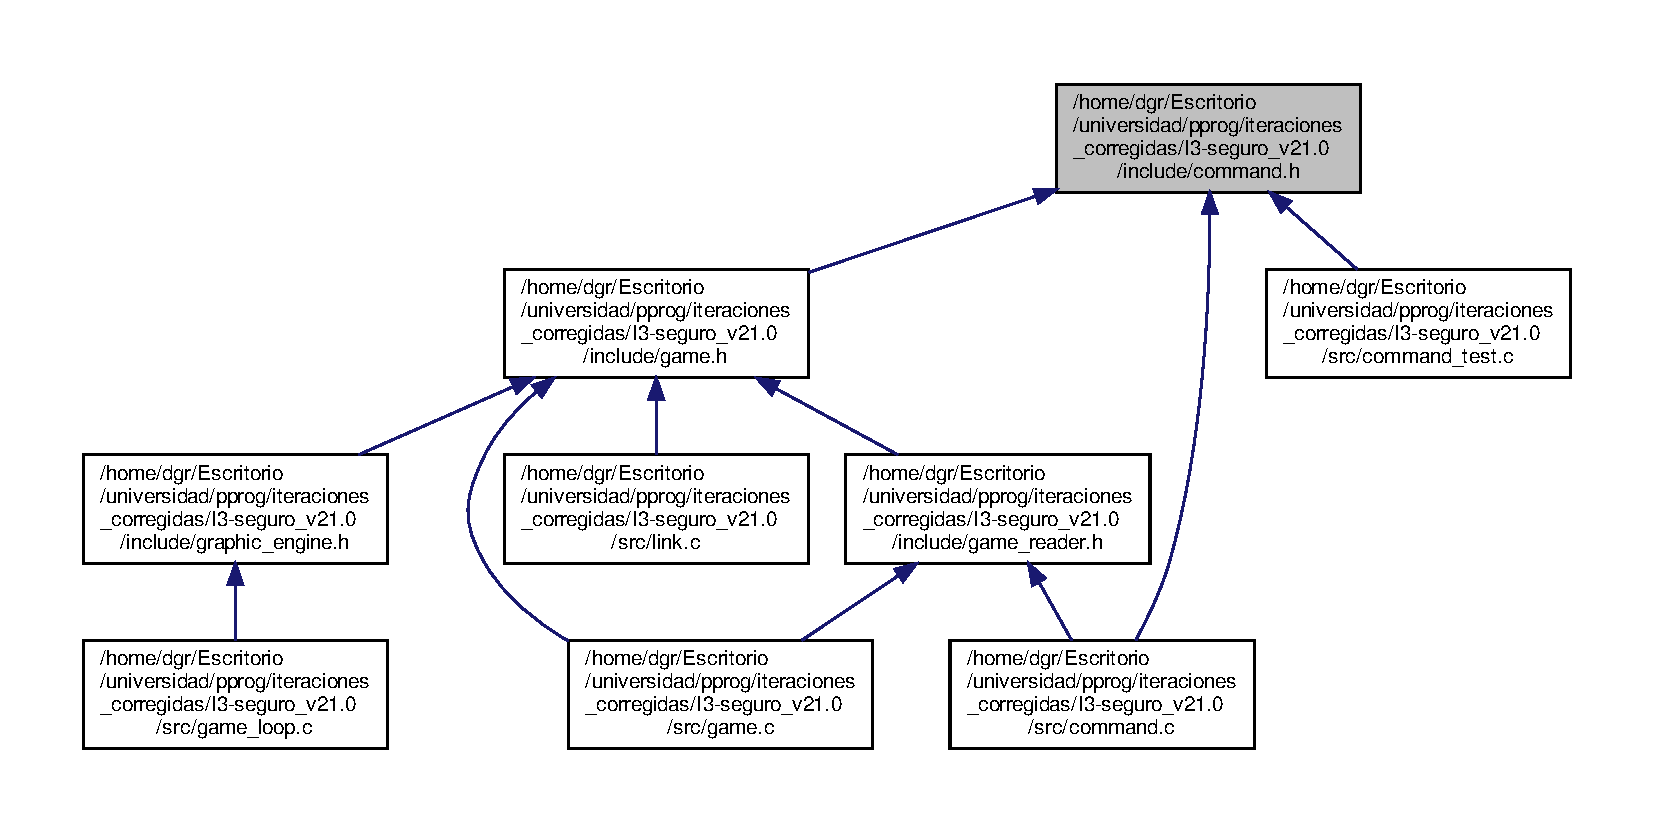
\includegraphics[width=350pt]{command_8h__dep__incl}
\end{center}
\end{figure}
\subsection*{Macros}
\begin{DoxyCompactItemize}
\item 
\#define \hyperlink{command_8h_a8d93932dcdc527c13e06b688b68c7ffc}{N\+\_\+\+C\+M\+DT}~2
\begin{DoxyCompactList}\small\item\em A macro that stores the number of commands types. \end{DoxyCompactList}\item 
\#define \hyperlink{command_8h_ae180fe89f0ae48ce5c80ffaa18de9271}{N\+\_\+\+C\+MD}~19
\begin{DoxyCompactList}\small\item\em A macro that stores the number of diferents commands. \end{DoxyCompactList}\item 
\#define \hyperlink{command_8h_a2b1bd24d2eddf8081d8c541e4cc4fd4b}{C\+M\+D\+\_\+\+L\+E\+N\+G\+HT}~30
\begin{DoxyCompactList}\small\item\em A macro that stores the maximum lenght of a cmd. \end{DoxyCompactList}\end{DoxyCompactItemize}
\subsection*{Typedefs}
\begin{DoxyCompactItemize}
\item 
typedef struct \hyperlink{struct__Command}{\+\_\+\+Command} \hyperlink{command_8h_a7d2935971c252377cb0fc1c8545dc2bc}{Command}
\begin{DoxyCompactList}\small\item\em A type definition for a command. \end{DoxyCompactList}\item 
\mbox{\Hypertarget{command_8h_a957aa66dcb0e0b6cdf162bb741f18c52}\label{command_8h_a957aa66dcb0e0b6cdf162bb741f18c52}} 
typedef enum \hyperlink{command_8h_a096a001f895e218ffb74047e101e6225}{enum\+\_\+\+Cmd\+Type} \hyperlink{command_8h_a957aa66dcb0e0b6cdf162bb741f18c52}{T\+\_\+\+Cmd\+Type}
\begin{DoxyCompactList}\small\item\em The Cmd\+Type enum. \end{DoxyCompactList}\item 
\mbox{\Hypertarget{command_8h_a0473597db8c45c0289b6b8e2f8abbe32}\label{command_8h_a0473597db8c45c0289b6b8e2f8abbe32}} 
typedef enum \hyperlink{command_8h_ace19ba2296a74e4aef53304e0934c50c}{enum\+\_\+\+Command} \hyperlink{command_8h_a0473597db8c45c0289b6b8e2f8abbe32}{T\+\_\+\+Command}
\begin{DoxyCompactList}\small\item\em The Command enum. \end{DoxyCompactList}\end{DoxyCompactItemize}
\subsection*{Enumerations}
\begin{DoxyCompactItemize}
\item 
\mbox{\Hypertarget{command_8h_a096a001f895e218ffb74047e101e6225}\label{command_8h_a096a001f895e218ffb74047e101e6225}} 
enum \hyperlink{command_8h_a096a001f895e218ffb74047e101e6225}{enum\+\_\+\+Cmd\+Type} \{ {\bfseries C\+M\+DS}, 
{\bfseries C\+M\+DL}
 \}\begin{DoxyCompactList}\small\item\em The Cmd\+Type enum. \end{DoxyCompactList}
\item 
\mbox{\Hypertarget{command_8h_ace19ba2296a74e4aef53304e0934c50c}\label{command_8h_ace19ba2296a74e4aef53304e0934c50c}} 
enum \hyperlink{command_8h_ace19ba2296a74e4aef53304e0934c50c}{enum\+\_\+\+Command} \{ \newline
{\bfseries N\+O\+\_\+\+C\+MD} = -\/1, 
{\bfseries U\+N\+K\+N\+O\+WN}, 
{\bfseries E\+X\+IT}, 
{\bfseries T\+A\+KE}, 
\newline
{\bfseries D\+R\+OP}, 
{\bfseries R\+O\+LL}, 
{\bfseries M\+O\+VE}, 
{\bfseries I\+N\+S\+P\+E\+CT}, 
\newline
{\bfseries T\+U\+R\+N\+ON}, 
{\bfseries T\+U\+R\+N\+O\+FF}, 
{\bfseries O\+P\+EN}, 
{\bfseries S\+A\+VE}, 
\newline
{\bfseries L\+O\+AD}, 
{\bfseries T\+A\+LK}, 
{\bfseries A\+C\+C\+U\+SE}, 
{\bfseries N\+E\+XT}, 
\newline
{\bfseries B\+A\+CK}, 
{\bfseries R\+I\+G\+HT}, 
{\bfseries L\+E\+FT}
 \}\begin{DoxyCompactList}\small\item\em The Command enum. \end{DoxyCompactList}
\end{DoxyCompactItemize}
\subsection*{Functions}
\begin{DoxyCompactItemize}
\item 
\hyperlink{command_8h_a7d2935971c252377cb0fc1c8545dc2bc}{Command} $\ast$ \hyperlink{command_8h_a25a96480a40811cf60e301f6d050fee3}{command\+\_\+init} ()
\begin{DoxyCompactList}\small\item\em initialitates the structure command command\+\_\+init \end{DoxyCompactList}\item 
\hyperlink{command_8h_a7d2935971c252377cb0fc1c8545dc2bc}{Command} $\ast$ \hyperlink{command_8h_a3bb1dc14827ec48c5e358d02cd909bc5}{command\+\_\+get\+\_\+user\+\_\+input} (\hyperlink{command_8h_a7d2935971c252377cb0fc1c8545dc2bc}{Command} $\ast$cmd)
\begin{DoxyCompactList}\small\item\em get the principal command and the argument \end{DoxyCompactList}\item 
\hyperlink{types_8h_a32c27cc471df37f4fc818d65de0a56c4}{S\+T\+A\+T\+US} \hyperlink{command_8h_a136c02c30eaf3dbaadcde50750ccafdc}{command\+\_\+set\+\_\+argument} (\hyperlink{command_8h_a7d2935971c252377cb0fc1c8545dc2bc}{Command} $\ast$cmd, char $\ast$argument)
\begin{DoxyCompactList}\small\item\em set an especific argument \end{DoxyCompactList}\item 
\hyperlink{types_8h_a32c27cc471df37f4fc818d65de0a56c4}{S\+T\+A\+T\+US} \hyperlink{command_8h_ae06b30b8f869f7236ce1abe8b5167b8d}{command\+\_\+set\+\_\+principalcmd} (\hyperlink{command_8h_a7d2935971c252377cb0fc1c8545dc2bc}{Command} $\ast$cmd, \hyperlink{command_8h_a0473597db8c45c0289b6b8e2f8abbe32}{T\+\_\+\+Command} command)
\begin{DoxyCompactList}\small\item\em set an especific command \end{DoxyCompactList}\item 
\hyperlink{types_8h_a32c27cc471df37f4fc818d65de0a56c4}{S\+T\+A\+T\+US} \hyperlink{command_8h_a7df71b69fa875de1b55df0174545807b}{command\+\_\+destroy} (\hyperlink{command_8h_a7d2935971c252377cb0fc1c8545dc2bc}{Command} $\ast$cmd)
\begin{DoxyCompactList}\small\item\em free the strcture command \end{DoxyCompactList}\item 
char $\ast$ \hyperlink{command_8h_a3392110efd7b39066a8aa5e6b4864ea8}{command\+\_\+get\+\_\+argument} (\hyperlink{command_8h_a7d2935971c252377cb0fc1c8545dc2bc}{Command} $\ast$cmd)
\begin{DoxyCompactList}\small\item\em get an argument \end{DoxyCompactList}\item 
\hyperlink{command_8h_a0473597db8c45c0289b6b8e2f8abbe32}{T\+\_\+\+Command} \hyperlink{command_8h_ad35081cca7cf7ff3161e48beb3a34624}{command\+\_\+get\+\_\+principalcmd} (\hyperlink{command_8h_a7d2935971c252377cb0fc1c8545dc2bc}{Command} $\ast$cmd)
\begin{DoxyCompactList}\small\item\em get the command \end{DoxyCompactList}\item 
\hyperlink{types_8h_a32c27cc471df37f4fc818d65de0a56c4}{S\+T\+A\+T\+US} \hyperlink{command_8h_ab28a732878a02cf27db4fd57c6d68daa}{command\+\_\+set\+\_\+status} (\hyperlink{command_8h_a7d2935971c252377cb0fc1c8545dc2bc}{Command} $\ast$cmd, char $\ast$status)
\begin{DoxyCompactList}\small\item\em set an especific status \end{DoxyCompactList}\item 
char $\ast$ \hyperlink{command_8h_a228fde7cd02041d88322fd5c676f1302}{command\+\_\+get\+\_\+status} (\hyperlink{command_8h_a7d2935971c252377cb0fc1c8545dc2bc}{Command} $\ast$cmd)
\begin{DoxyCompactList}\small\item\em get an especific status \end{DoxyCompactList}\end{DoxyCompactItemize}


\subsection{Detailed Description}
It implements the command interpreter. 

\begin{DoxyAuthor}{Author}
José Manuel García Giráldez, David Teófilo Garitagoitia Romero 
\end{DoxyAuthor}
\begin{DoxyVersion}{Version}
1.\+0 
\end{DoxyVersion}
\begin{DoxyDate}{Date}
19-\/12-\/2014 
\end{DoxyDate}
\begin{DoxyCopyright}{Copyright}
G\+NU Public License 
\end{DoxyCopyright}


\subsection{Macro Definition Documentation}
\mbox{\Hypertarget{command_8h_a2b1bd24d2eddf8081d8c541e4cc4fd4b}\label{command_8h_a2b1bd24d2eddf8081d8c541e4cc4fd4b}} 
\index{command.\+h@{command.\+h}!C\+M\+D\+\_\+\+L\+E\+N\+G\+HT@{C\+M\+D\+\_\+\+L\+E\+N\+G\+HT}}
\index{C\+M\+D\+\_\+\+L\+E\+N\+G\+HT@{C\+M\+D\+\_\+\+L\+E\+N\+G\+HT}!command.\+h@{command.\+h}}
\subsubsection{\texorpdfstring{C\+M\+D\+\_\+\+L\+E\+N\+G\+HT}{CMD\_LENGHT}}
{\footnotesize\ttfamily \#define C\+M\+D\+\_\+\+L\+E\+N\+G\+HT~30}



A macro that stores the maximum lenght of a cmd. 

Details. \mbox{\Hypertarget{command_8h_ae180fe89f0ae48ce5c80ffaa18de9271}\label{command_8h_ae180fe89f0ae48ce5c80ffaa18de9271}} 
\index{command.\+h@{command.\+h}!N\+\_\+\+C\+MD@{N\+\_\+\+C\+MD}}
\index{N\+\_\+\+C\+MD@{N\+\_\+\+C\+MD}!command.\+h@{command.\+h}}
\subsubsection{\texorpdfstring{N\+\_\+\+C\+MD}{N\_CMD}}
{\footnotesize\ttfamily \#define N\+\_\+\+C\+MD~19}



A macro that stores the number of diferents commands. 

Details. \mbox{\Hypertarget{command_8h_a8d93932dcdc527c13e06b688b68c7ffc}\label{command_8h_a8d93932dcdc527c13e06b688b68c7ffc}} 
\index{command.\+h@{command.\+h}!N\+\_\+\+C\+M\+DT@{N\+\_\+\+C\+M\+DT}}
\index{N\+\_\+\+C\+M\+DT@{N\+\_\+\+C\+M\+DT}!command.\+h@{command.\+h}}
\subsubsection{\texorpdfstring{N\+\_\+\+C\+M\+DT}{N\_CMDT}}
{\footnotesize\ttfamily \#define N\+\_\+\+C\+M\+DT~2}



A macro that stores the number of commands types. 

Details. 

\subsection{Typedef Documentation}
\mbox{\Hypertarget{command_8h_a7d2935971c252377cb0fc1c8545dc2bc}\label{command_8h_a7d2935971c252377cb0fc1c8545dc2bc}} 
\index{command.\+h@{command.\+h}!Command@{Command}}
\index{Command@{Command}!command.\+h@{command.\+h}}
\subsubsection{\texorpdfstring{Command}{Command}}
{\footnotesize\ttfamily typedef struct \hyperlink{struct__Command}{\+\_\+\+Command} \hyperlink{command_8h_a7d2935971c252377cb0fc1c8545dc2bc}{Command}}



A type definition for a command. 

Details. 

\subsection{Function Documentation}
\mbox{\Hypertarget{command_8h_a7df71b69fa875de1b55df0174545807b}\label{command_8h_a7df71b69fa875de1b55df0174545807b}} 
\index{command.\+h@{command.\+h}!command\+\_\+destroy@{command\+\_\+destroy}}
\index{command\+\_\+destroy@{command\+\_\+destroy}!command.\+h@{command.\+h}}
\subsubsection{\texorpdfstring{command\+\_\+destroy()}{command\_destroy()}}
{\footnotesize\ttfamily \hyperlink{types_8h_a32c27cc471df37f4fc818d65de0a56c4}{S\+T\+A\+T\+US} command\+\_\+destroy (\begin{DoxyParamCaption}\item[{\hyperlink{command_8h_a7d2935971c252377cb0fc1c8545dc2bc}{Command} $\ast$}]{cmd }\end{DoxyParamCaption})}



free the strcture command 

command\+\_\+destroy

\begin{DoxyDate}{Date}
06-\/03-\/2019 
\end{DoxyDate}
\begin{DoxyAuthor}{Author}
José Manuel García Giráldez 
\end{DoxyAuthor}

\begin{DoxyParams}{Parameters}
{\em cmd} & the command structure \\
\hline
\end{DoxyParams}
\begin{DoxyReturn}{Returns}
E\+R\+R\+OR if there is an error, otherwise return OK 
\end{DoxyReturn}
\mbox{\Hypertarget{command_8h_a3392110efd7b39066a8aa5e6b4864ea8}\label{command_8h_a3392110efd7b39066a8aa5e6b4864ea8}} 
\index{command.\+h@{command.\+h}!command\+\_\+get\+\_\+argument@{command\+\_\+get\+\_\+argument}}
\index{command\+\_\+get\+\_\+argument@{command\+\_\+get\+\_\+argument}!command.\+h@{command.\+h}}
\subsubsection{\texorpdfstring{command\+\_\+get\+\_\+argument()}{command\_get\_argument()}}
{\footnotesize\ttfamily char$\ast$ command\+\_\+get\+\_\+argument (\begin{DoxyParamCaption}\item[{\hyperlink{command_8h_a7d2935971c252377cb0fc1c8545dc2bc}{Command} $\ast$}]{cmd }\end{DoxyParamCaption})}



get an argument 

command\+\_\+get\+\_\+argument

\begin{DoxyDate}{Date}
06-\/03-\/2019 
\end{DoxyDate}
\begin{DoxyAuthor}{Author}
José Manuel García Giráldez 
\end{DoxyAuthor}

\begin{DoxyParams}{Parameters}
{\em cmd} & the command structure \\
\hline
\end{DoxyParams}
\begin{DoxyReturn}{Returns}
the argument 
\end{DoxyReturn}
\mbox{\Hypertarget{command_8h_ad35081cca7cf7ff3161e48beb3a34624}\label{command_8h_ad35081cca7cf7ff3161e48beb3a34624}} 
\index{command.\+h@{command.\+h}!command\+\_\+get\+\_\+principalcmd@{command\+\_\+get\+\_\+principalcmd}}
\index{command\+\_\+get\+\_\+principalcmd@{command\+\_\+get\+\_\+principalcmd}!command.\+h@{command.\+h}}
\subsubsection{\texorpdfstring{command\+\_\+get\+\_\+principalcmd()}{command\_get\_principalcmd()}}
{\footnotesize\ttfamily \hyperlink{command_8h_a0473597db8c45c0289b6b8e2f8abbe32}{T\+\_\+\+Command} command\+\_\+get\+\_\+principalcmd (\begin{DoxyParamCaption}\item[{\hyperlink{command_8h_a7d2935971c252377cb0fc1c8545dc2bc}{Command} $\ast$}]{cmd }\end{DoxyParamCaption})}



get the command 

command\+\_\+get\+\_\+principalcmd

\begin{DoxyDate}{Date}
06-\/03-\/2019 
\end{DoxyDate}
\begin{DoxyAuthor}{Author}
José Manuel García Giráldez 
\end{DoxyAuthor}

\begin{DoxyParams}{Parameters}
{\em cmd} & the command structure \\
\hline
\end{DoxyParams}
\begin{DoxyReturn}{Returns}
the command 
\end{DoxyReturn}
\mbox{\Hypertarget{command_8h_a228fde7cd02041d88322fd5c676f1302}\label{command_8h_a228fde7cd02041d88322fd5c676f1302}} 
\index{command.\+h@{command.\+h}!command\+\_\+get\+\_\+status@{command\+\_\+get\+\_\+status}}
\index{command\+\_\+get\+\_\+status@{command\+\_\+get\+\_\+status}!command.\+h@{command.\+h}}
\subsubsection{\texorpdfstring{command\+\_\+get\+\_\+status()}{command\_get\_status()}}
{\footnotesize\ttfamily char$\ast$ command\+\_\+get\+\_\+status (\begin{DoxyParamCaption}\item[{\hyperlink{command_8h_a7d2935971c252377cb0fc1c8545dc2bc}{Command} $\ast$}]{cmd }\end{DoxyParamCaption})}



get an especific status 

command\+\_\+get\+\_\+status

\begin{DoxyDate}{Date}
06-\/03-\/2019 
\end{DoxyDate}
\begin{DoxyAuthor}{Author}
David Teófilo Garitagoitia Romero 
\end{DoxyAuthor}

\begin{DoxyParams}{Parameters}
{\em cmd} & the command structure \\
\hline
\end{DoxyParams}
\begin{DoxyReturn}{Returns}
N\+U\+LL if there is an error, otherwise return the status 
\end{DoxyReturn}
\mbox{\Hypertarget{command_8h_a3bb1dc14827ec48c5e358d02cd909bc5}\label{command_8h_a3bb1dc14827ec48c5e358d02cd909bc5}} 
\index{command.\+h@{command.\+h}!command\+\_\+get\+\_\+user\+\_\+input@{command\+\_\+get\+\_\+user\+\_\+input}}
\index{command\+\_\+get\+\_\+user\+\_\+input@{command\+\_\+get\+\_\+user\+\_\+input}!command.\+h@{command.\+h}}
\subsubsection{\texorpdfstring{command\+\_\+get\+\_\+user\+\_\+input()}{command\_get\_user\_input()}}
{\footnotesize\ttfamily \hyperlink{command_8h_a7d2935971c252377cb0fc1c8545dc2bc}{Command}$\ast$ command\+\_\+get\+\_\+user\+\_\+input (\begin{DoxyParamCaption}\item[{\hyperlink{command_8h_a7d2935971c252377cb0fc1c8545dc2bc}{Command} $\ast$}]{cmd }\end{DoxyParamCaption})}



get the principal command and the argument 

command\+\_\+get\+\_\+user\+\_\+input

\begin{DoxyDate}{Date}
06-\/03-\/2019 
\end{DoxyDate}
\begin{DoxyAuthor}{Author}
José Manuel García Giráldez 
\end{DoxyAuthor}

\begin{DoxyParams}{Parameters}
{\em cmd} & the command structure and file to log \\
\hline
\end{DoxyParams}
\begin{DoxyReturn}{Returns}
the structure command 
\end{DoxyReturn}
\mbox{\Hypertarget{command_8h_a25a96480a40811cf60e301f6d050fee3}\label{command_8h_a25a96480a40811cf60e301f6d050fee3}} 
\index{command.\+h@{command.\+h}!command\+\_\+init@{command\+\_\+init}}
\index{command\+\_\+init@{command\+\_\+init}!command.\+h@{command.\+h}}
\subsubsection{\texorpdfstring{command\+\_\+init()}{command\_init()}}
{\footnotesize\ttfamily \hyperlink{command_8h_a7d2935971c252377cb0fc1c8545dc2bc}{Command}$\ast$ command\+\_\+init (\begin{DoxyParamCaption}{ }\end{DoxyParamCaption})}



initialitates the structure command command\+\_\+init 

\begin{DoxyDate}{Date}
06-\/03-\/2019 
\end{DoxyDate}
\begin{DoxyAuthor}{Author}
José Manuel García Giráldez 
\end{DoxyAuthor}
\begin{DoxyReturn}{Returns}
the structure command 
\end{DoxyReturn}
\mbox{\Hypertarget{command_8h_a136c02c30eaf3dbaadcde50750ccafdc}\label{command_8h_a136c02c30eaf3dbaadcde50750ccafdc}} 
\index{command.\+h@{command.\+h}!command\+\_\+set\+\_\+argument@{command\+\_\+set\+\_\+argument}}
\index{command\+\_\+set\+\_\+argument@{command\+\_\+set\+\_\+argument}!command.\+h@{command.\+h}}
\subsubsection{\texorpdfstring{command\+\_\+set\+\_\+argument()}{command\_set\_argument()}}
{\footnotesize\ttfamily \hyperlink{types_8h_a32c27cc471df37f4fc818d65de0a56c4}{S\+T\+A\+T\+US} command\+\_\+set\+\_\+argument (\begin{DoxyParamCaption}\item[{\hyperlink{command_8h_a7d2935971c252377cb0fc1c8545dc2bc}{Command} $\ast$}]{cmd,  }\item[{char $\ast$}]{argument }\end{DoxyParamCaption})}



set an especific argument 

command\+\_\+set\+\_\+argument

\begin{DoxyDate}{Date}
06-\/03-\/2019 
\end{DoxyDate}
\begin{DoxyAuthor}{Author}
José Manuel García Giráldez 
\end{DoxyAuthor}

\begin{DoxyParams}{Parameters}
{\em cmd} & the command structure \\
\hline
{\em argument} & the argument we want to set \\
\hline
\end{DoxyParams}
\begin{DoxyReturn}{Returns}
E\+R\+R\+OR if there is an error, otherwise return OK 
\end{DoxyReturn}
\mbox{\Hypertarget{command_8h_ae06b30b8f869f7236ce1abe8b5167b8d}\label{command_8h_ae06b30b8f869f7236ce1abe8b5167b8d}} 
\index{command.\+h@{command.\+h}!command\+\_\+set\+\_\+principalcmd@{command\+\_\+set\+\_\+principalcmd}}
\index{command\+\_\+set\+\_\+principalcmd@{command\+\_\+set\+\_\+principalcmd}!command.\+h@{command.\+h}}
\subsubsection{\texorpdfstring{command\+\_\+set\+\_\+principalcmd()}{command\_set\_principalcmd()}}
{\footnotesize\ttfamily \hyperlink{types_8h_a32c27cc471df37f4fc818d65de0a56c4}{S\+T\+A\+T\+US} command\+\_\+set\+\_\+principalcmd (\begin{DoxyParamCaption}\item[{\hyperlink{command_8h_a7d2935971c252377cb0fc1c8545dc2bc}{Command} $\ast$}]{cmd,  }\item[{\hyperlink{command_8h_a0473597db8c45c0289b6b8e2f8abbe32}{T\+\_\+\+Command}}]{command }\end{DoxyParamCaption})}



set an especific command 

command\+\_\+set\+\_\+principalcmd

\begin{DoxyDate}{Date}
06-\/03-\/2019 
\end{DoxyDate}
\begin{DoxyAuthor}{Author}
José Manuel García Giráldez 
\end{DoxyAuthor}

\begin{DoxyParams}{Parameters}
{\em cmd} & the command structure \\
\hline
{\em command} & the command we want to set \\
\hline
\end{DoxyParams}
\begin{DoxyReturn}{Returns}
E\+R\+R\+OR if there is an error, otherwise return OK 
\end{DoxyReturn}
\mbox{\Hypertarget{command_8h_ab28a732878a02cf27db4fd57c6d68daa}\label{command_8h_ab28a732878a02cf27db4fd57c6d68daa}} 
\index{command.\+h@{command.\+h}!command\+\_\+set\+\_\+status@{command\+\_\+set\+\_\+status}}
\index{command\+\_\+set\+\_\+status@{command\+\_\+set\+\_\+status}!command.\+h@{command.\+h}}
\subsubsection{\texorpdfstring{command\+\_\+set\+\_\+status()}{command\_set\_status()}}
{\footnotesize\ttfamily \hyperlink{types_8h_a32c27cc471df37f4fc818d65de0a56c4}{S\+T\+A\+T\+US} command\+\_\+set\+\_\+status (\begin{DoxyParamCaption}\item[{\hyperlink{command_8h_a7d2935971c252377cb0fc1c8545dc2bc}{Command} $\ast$}]{cmd,  }\item[{char $\ast$}]{status }\end{DoxyParamCaption})}



set an especific status 

command\+\_\+set\+\_\+status

\begin{DoxyDate}{Date}
06-\/03-\/2019 
\end{DoxyDate}
\begin{DoxyAuthor}{Author}
David Teófilo Garitagoitia Romero 
\end{DoxyAuthor}

\begin{DoxyParams}{Parameters}
{\em cmd} & the command structure \\
\hline
{\em status} & the status we want to set \\
\hline
\end{DoxyParams}
\begin{DoxyReturn}{Returns}
E\+R\+R\+OR if there is an error, otherwise return OK 
\end{DoxyReturn}

\hypertarget{command__test_8h}{}\section{/home/dgr/\+Escritorio/universidad/pprog/iteraciones\+\_\+corregidas/\+I3-\/seguro\+\_\+v21.0/include/command\+\_\+test.h File Reference}
\label{command__test_8h}\index{/home/dgr/\+Escritorio/universidad/pprog/iteraciones\+\_\+corregidas/\+I3-\/seguro\+\_\+v21.\+0/include/command\+\_\+test.\+h@{/home/dgr/\+Escritorio/universidad/pprog/iteraciones\+\_\+corregidas/\+I3-\/seguro\+\_\+v21.\+0/include/command\+\_\+test.\+h}}


It declares the tests for the command module.  


This graph shows which files directly or indirectly include this file\+:
\nopagebreak
\begin{figure}[H]
\begin{center}
\leavevmode
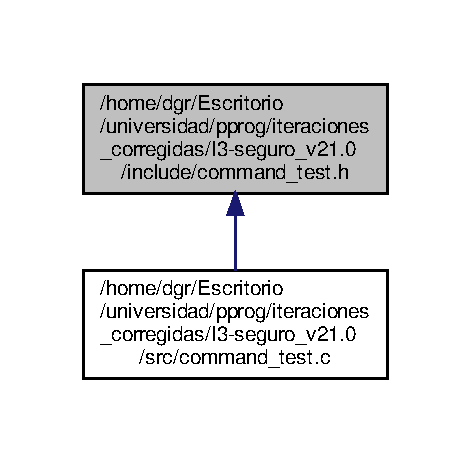
\includegraphics[width=226pt]{command__test_8h__dep__incl}
\end{center}
\end{figure}
\subsection*{Functions}
\begin{DoxyCompactItemize}
\item 
void \hyperlink{command__test_8h_af91aeb3bc73f994f5214b8954f3c4797}{test1\+\_\+command\+\_\+init} ()
\item 
void \hyperlink{command__test_8h_a084363877b09c47c4167fb675ba0a6c5}{test2\+\_\+command\+\_\+init} ()
\item 
void \hyperlink{command__test_8h_a1d44a3ed59cc78359d6c8c0d720347e1}{test3\+\_\+command\+\_\+init} ()
\item 
void \hyperlink{command__test_8h_a6367528b38336d716e765ea2d57f6d8c}{test4\+\_\+command\+\_\+init} ()
\item 
void \hyperlink{command__test_8h_a4e6817b2faaa57ed732eb9a68e671ef1}{test1\+\_\+command\+\_\+set\+\_\+principal\+\_\+cmd} ()
\item 
void \hyperlink{command__test_8h_a2f897a338775789b9e1b0b8a8647fd85}{test2\+\_\+command\+\_\+set\+\_\+principal\+\_\+cmd} ()
\item 
void \hyperlink{command__test_8h_a7e2613ae40c77091d31e9dd549c5d848}{test3\+\_\+command\+\_\+set\+\_\+principal\+\_\+cmd} ()
\item 
void \hyperlink{command__test_8h_a0485be612e6f281fe6e5b4dc778e2b72}{test4\+\_\+command\+\_\+set\+\_\+principal\+\_\+cmd} ()
\item 
void \hyperlink{command__test_8h_aa9706a5391086cfb6daf56613b55b351}{test5\+\_\+command\+\_\+set\+\_\+principal\+\_\+cmd} ()
\item 
void \hyperlink{command__test_8h_a1fd80f6afee487d3aa0386b22e85ac38}{test6\+\_\+command\+\_\+set\+\_\+principal\+\_\+cmd} ()
\item 
void \hyperlink{command__test_8h_aaacb4bcd77193d1e88615373040ea9a5}{test7\+\_\+command\+\_\+set\+\_\+principal\+\_\+cmd} ()
\item 
void \hyperlink{command__test_8h_a3c00c13f79566dca26966f011cdcb9b5}{test8\+\_\+command\+\_\+set\+\_\+principal\+\_\+cmd} ()
\item 
void \hyperlink{command__test_8h_af037a9eb46fd5e7700ec1f0760a5b9ec}{test9\+\_\+command\+\_\+set\+\_\+principal\+\_\+cmd} ()
\item 
void \hyperlink{command__test_8h_aba7be3a0f6ef3e6717088a21d32e9a21}{test10\+\_\+command\+\_\+set\+\_\+principal\+\_\+cmd} ()
\item 
void \hyperlink{command__test_8h_ae492f21ffdf46fc9380339f397f12675}{test11\+\_\+command\+\_\+set\+\_\+principal\+\_\+cmd} ()
\item 
void \hyperlink{command__test_8h_ab42210ac5001729f927be902384c51c6}{test12\+\_\+command\+\_\+set\+\_\+principal\+\_\+cmd} ()
\item 
void \hyperlink{command__test_8h_a86c724b0ce8b1a19b138fb1cb5dd84e3}{test1\+\_\+command\+\_\+set\+\_\+status} ()
\item 
void \hyperlink{command__test_8h_a67ea36686a450269ef95eace71e78867}{test2\+\_\+command\+\_\+set\+\_\+status} ()
\item 
void \hyperlink{command__test_8h_a5c554b37bf888c3077aa310982cedf14}{test3\+\_\+command\+\_\+set\+\_\+status} ()
\item 
void \hyperlink{command__test_8h_a88a8e8dddaca55194bd73c4d6796ec9b}{test1\+\_\+command\+\_\+set\+\_\+argument} ()
\item 
void \hyperlink{command__test_8h_a66f78c148ff91ffcbaa521f00d208a75}{test2\+\_\+command\+\_\+set\+\_\+argument} ()
\item 
void \hyperlink{command__test_8h_a69324b158668120d802451ce7c951d9e}{test3\+\_\+command\+\_\+set\+\_\+argument} ()
\item 
void \hyperlink{command__test_8h_aadf731a98e5122e70ede7cdc68ba621f}{test1\+\_\+command\+\_\+destroy} ()
\item 
void \hyperlink{command__test_8h_ad445f3e81035d4ab32ebc1526eb83fcb}{test2\+\_\+command\+\_\+destroy} ()
\item 
void \hyperlink{command__test_8h_a932afa8fb63c9b8ba551d030886ce491}{test1\+\_\+command\+\_\+get\+\_\+user\+\_\+input} ()
\item 
void \hyperlink{command__test_8h_a3ba7658db8aa069706b344d42ceabfaa}{test2\+\_\+command\+\_\+get\+\_\+user\+\_\+input} ()
\item 
void \hyperlink{command__test_8h_ae2d4b758fa9767317795c822b7334dec}{test3\+\_\+command\+\_\+get\+\_\+user\+\_\+input} ()
\item 
void \hyperlink{command__test_8h_a87e1a266b9beb6b31dd8e626694d5dd6}{test4\+\_\+command\+\_\+get\+\_\+user\+\_\+input} ()
\item 
void \hyperlink{command__test_8h_a3b7a4bfd103971720b0daef936b9251c}{test5\+\_\+command\+\_\+get\+\_\+user\+\_\+input} ()
\item 
void \hyperlink{command__test_8h_a85a9509e4435960ab89a0968666c2588}{test6\+\_\+command\+\_\+get\+\_\+user\+\_\+input} ()
\item 
void \hyperlink{command__test_8h_ab3a94f10959f43dca5f3a1254d2455a4}{test7\+\_\+command\+\_\+get\+\_\+user\+\_\+input} ()
\item 
void \hyperlink{command__test_8h_a96e8d3216af1419e01aaa68052a4ed26}{test8\+\_\+command\+\_\+get\+\_\+user\+\_\+input} ()
\item 
void \hyperlink{command__test_8h_ad9250b3696fed0b765bc703ecfa06066}{test9\+\_\+command\+\_\+get\+\_\+user\+\_\+input} ()
\item 
void \hyperlink{command__test_8h_a5a8b71fe0575431c76639d1a1703dd56}{test10\+\_\+command\+\_\+get\+\_\+user\+\_\+input} ()
\item 
void \hyperlink{command__test_8h_ada1f2861adf1a95726d5d08ecf6c015a}{test11\+\_\+command\+\_\+get\+\_\+user\+\_\+input} ()
\item 
void \hyperlink{command__test_8h_a01d0cd8d45e24b2b1a455a4ab50654cd}{test12\+\_\+command\+\_\+get\+\_\+user\+\_\+input} ()
\item 
void \hyperlink{command__test_8h_a274781536f1262b9c22ee97c1a57af18}{test13\+\_\+command\+\_\+get\+\_\+user\+\_\+input} ()
\item 
void \hyperlink{command__test_8h_a8f9bd7fc5112b6851b4e77a785984858}{test14\+\_\+command\+\_\+get\+\_\+user\+\_\+input} ()
\item 
void \hyperlink{command__test_8h_ae901b403f53f05148d2183d8205f968c}{test15\+\_\+command\+\_\+get\+\_\+user\+\_\+input} ()
\item 
void \hyperlink{command__test_8h_a9acb10b7ed10138a24190b90358e0583}{test16\+\_\+command\+\_\+get\+\_\+user\+\_\+input} ()
\item 
void \hyperlink{command__test_8h_a46ab7fb8f1c83596debe331b2c7bfbe0}{test17\+\_\+command\+\_\+get\+\_\+user\+\_\+input} ()
\item 
void \hyperlink{command__test_8h_a4db087cfa5bf22f248747b748745379f}{test18\+\_\+command\+\_\+get\+\_\+user\+\_\+input} ()
\item 
void \hyperlink{command__test_8h_a340bc65a10e7f7bdcddcef019bbd5aa7}{test19\+\_\+command\+\_\+get\+\_\+user\+\_\+input} ()
\item 
void \hyperlink{command__test_8h_a92cce7477f40656ebebe28d56142b528}{test20\+\_\+command\+\_\+get\+\_\+user\+\_\+input} ()
\item 
void \hyperlink{command__test_8h_aaf02a6c7423e84f000c00b8218a8a9a1}{test21\+\_\+command\+\_\+get\+\_\+user\+\_\+input} ()
\item 
void \hyperlink{command__test_8h_ac1ff85e1d54f46eccdbdaffec062d5c0}{test22\+\_\+command\+\_\+get\+\_\+user\+\_\+input} ()
\item 
void \hyperlink{command__test_8h_a618f500cde2987b4f746357b2a990b69}{test23\+\_\+command\+\_\+get\+\_\+user\+\_\+input} ()
\end{DoxyCompactItemize}


\subsection{Detailed Description}
It declares the tests for the command module. 

\begin{DoxyAuthor}{Author}
David Teófilo Garitagoitia Romero 
\end{DoxyAuthor}
\begin{DoxyVersion}{Version}
1.\+0 
\end{DoxyVersion}
\begin{DoxyDate}{Date}
10-\/06-\/2020 
\end{DoxyDate}
\begin{DoxyCopyright}{Copyright}
G\+NU Public License 
\end{DoxyCopyright}


\subsection{Function Documentation}
\mbox{\Hypertarget{command__test_8h_a5a8b71fe0575431c76639d1a1703dd56}\label{command__test_8h_a5a8b71fe0575431c76639d1a1703dd56}} 
\index{command\+\_\+test.\+h@{command\+\_\+test.\+h}!test10\+\_\+command\+\_\+get\+\_\+user\+\_\+input@{test10\+\_\+command\+\_\+get\+\_\+user\+\_\+input}}
\index{test10\+\_\+command\+\_\+get\+\_\+user\+\_\+input@{test10\+\_\+command\+\_\+get\+\_\+user\+\_\+input}!command\+\_\+test.\+h@{command\+\_\+test.\+h}}
\subsubsection{\texorpdfstring{test10\+\_\+command\+\_\+get\+\_\+user\+\_\+input()}{test10\_command\_get\_user\_input()}}
{\footnotesize\ttfamily void test10\+\_\+command\+\_\+get\+\_\+user\+\_\+input (\begin{DoxyParamCaption}{ }\end{DoxyParamCaption})}

\begin{DoxyRefDesc}{Test}
\item[\hyperlink{test__test000034}{Test}]Test the command get user input function \end{DoxyRefDesc}
\begin{DoxyPrecond}{Precondition}
Use the text file with the instructions, in this case, the instruction is m n (move and the argument is n) 
\end{DoxyPrecond}
\begin{DoxyPostcond}{Postcondition}
The principal cmd must be move and the argument must be n 
\end{DoxyPostcond}
\mbox{\Hypertarget{command__test_8h_aba7be3a0f6ef3e6717088a21d32e9a21}\label{command__test_8h_aba7be3a0f6ef3e6717088a21d32e9a21}} 
\index{command\+\_\+test.\+h@{command\+\_\+test.\+h}!test10\+\_\+command\+\_\+set\+\_\+principal\+\_\+cmd@{test10\+\_\+command\+\_\+set\+\_\+principal\+\_\+cmd}}
\index{test10\+\_\+command\+\_\+set\+\_\+principal\+\_\+cmd@{test10\+\_\+command\+\_\+set\+\_\+principal\+\_\+cmd}!command\+\_\+test.\+h@{command\+\_\+test.\+h}}
\subsubsection{\texorpdfstring{test10\+\_\+command\+\_\+set\+\_\+principal\+\_\+cmd()}{test10\_command\_set\_principal\_cmd()}}
{\footnotesize\ttfamily void test10\+\_\+command\+\_\+set\+\_\+principal\+\_\+cmd (\begin{DoxyParamCaption}{ }\end{DoxyParamCaption})}

\begin{DoxyRefDesc}{Test}
\item[\hyperlink{test__test000014}{Test}]Test the command set principal cmd function \end{DoxyRefDesc}
\begin{DoxyPrecond}{Precondition}
An cmd as a parameter 
\end{DoxyPrecond}
\begin{DoxyPostcond}{Postcondition}
The principal cmd must be B\+A\+CK 
\end{DoxyPostcond}
\mbox{\Hypertarget{command__test_8h_ada1f2861adf1a95726d5d08ecf6c015a}\label{command__test_8h_ada1f2861adf1a95726d5d08ecf6c015a}} 
\index{command\+\_\+test.\+h@{command\+\_\+test.\+h}!test11\+\_\+command\+\_\+get\+\_\+user\+\_\+input@{test11\+\_\+command\+\_\+get\+\_\+user\+\_\+input}}
\index{test11\+\_\+command\+\_\+get\+\_\+user\+\_\+input@{test11\+\_\+command\+\_\+get\+\_\+user\+\_\+input}!command\+\_\+test.\+h@{command\+\_\+test.\+h}}
\subsubsection{\texorpdfstring{test11\+\_\+command\+\_\+get\+\_\+user\+\_\+input()}{test11\_command\_get\_user\_input()}}
{\footnotesize\ttfamily void test11\+\_\+command\+\_\+get\+\_\+user\+\_\+input (\begin{DoxyParamCaption}{ }\end{DoxyParamCaption})}

\begin{DoxyRefDesc}{Test}
\item[\hyperlink{test__test000035}{Test}]Test the command get user input function \end{DoxyRefDesc}
\begin{DoxyPrecond}{Precondition}
Use the text file with the instructions, in this case, the instruction is move south (move and the argument is south) 
\end{DoxyPrecond}
\begin{DoxyPostcond}{Postcondition}
The principal cmd must be move and the argument must be south 
\end{DoxyPostcond}
\mbox{\Hypertarget{command__test_8h_ae492f21ffdf46fc9380339f397f12675}\label{command__test_8h_ae492f21ffdf46fc9380339f397f12675}} 
\index{command\+\_\+test.\+h@{command\+\_\+test.\+h}!test11\+\_\+command\+\_\+set\+\_\+principal\+\_\+cmd@{test11\+\_\+command\+\_\+set\+\_\+principal\+\_\+cmd}}
\index{test11\+\_\+command\+\_\+set\+\_\+principal\+\_\+cmd@{test11\+\_\+command\+\_\+set\+\_\+principal\+\_\+cmd}!command\+\_\+test.\+h@{command\+\_\+test.\+h}}
\subsubsection{\texorpdfstring{test11\+\_\+command\+\_\+set\+\_\+principal\+\_\+cmd()}{test11\_command\_set\_principal\_cmd()}}
{\footnotesize\ttfamily void test11\+\_\+command\+\_\+set\+\_\+principal\+\_\+cmd (\begin{DoxyParamCaption}{ }\end{DoxyParamCaption})}

\begin{DoxyRefDesc}{Test}
\item[\hyperlink{test__test000015}{Test}]Test the command set principal cmd function \end{DoxyRefDesc}
\begin{DoxyPrecond}{Precondition}
An cmd as a parameter 
\end{DoxyPrecond}
\begin{DoxyPostcond}{Postcondition}
The principal cmd must be R\+I\+G\+HT 
\end{DoxyPostcond}
\mbox{\Hypertarget{command__test_8h_a01d0cd8d45e24b2b1a455a4ab50654cd}\label{command__test_8h_a01d0cd8d45e24b2b1a455a4ab50654cd}} 
\index{command\+\_\+test.\+h@{command\+\_\+test.\+h}!test12\+\_\+command\+\_\+get\+\_\+user\+\_\+input@{test12\+\_\+command\+\_\+get\+\_\+user\+\_\+input}}
\index{test12\+\_\+command\+\_\+get\+\_\+user\+\_\+input@{test12\+\_\+command\+\_\+get\+\_\+user\+\_\+input}!command\+\_\+test.\+h@{command\+\_\+test.\+h}}
\subsubsection{\texorpdfstring{test12\+\_\+command\+\_\+get\+\_\+user\+\_\+input()}{test12\_command\_get\_user\_input()}}
{\footnotesize\ttfamily void test12\+\_\+command\+\_\+get\+\_\+user\+\_\+input (\begin{DoxyParamCaption}{ }\end{DoxyParamCaption})}

\begin{DoxyRefDesc}{Test}
\item[\hyperlink{test__test000036}{Test}]Test the command get user input function \end{DoxyRefDesc}
\begin{DoxyPrecond}{Precondition}
Use the text file with the instructions, in this case, the instruction is n next (next) 
\end{DoxyPrecond}
\begin{DoxyPostcond}{Postcondition}
The principal cmd must be next and the argument must be \char`\"{}\textbackslash{}0\char`\"{} 
\end{DoxyPostcond}
\mbox{\Hypertarget{command__test_8h_ab42210ac5001729f927be902384c51c6}\label{command__test_8h_ab42210ac5001729f927be902384c51c6}} 
\index{command\+\_\+test.\+h@{command\+\_\+test.\+h}!test12\+\_\+command\+\_\+set\+\_\+principal\+\_\+cmd@{test12\+\_\+command\+\_\+set\+\_\+principal\+\_\+cmd}}
\index{test12\+\_\+command\+\_\+set\+\_\+principal\+\_\+cmd@{test12\+\_\+command\+\_\+set\+\_\+principal\+\_\+cmd}!command\+\_\+test.\+h@{command\+\_\+test.\+h}}
\subsubsection{\texorpdfstring{test12\+\_\+command\+\_\+set\+\_\+principal\+\_\+cmd()}{test12\_command\_set\_principal\_cmd()}}
{\footnotesize\ttfamily void test12\+\_\+command\+\_\+set\+\_\+principal\+\_\+cmd (\begin{DoxyParamCaption}{ }\end{DoxyParamCaption})}

\begin{DoxyRefDesc}{Test}
\item[\hyperlink{test__test000016}{Test}]Test the command set principal cmd function \end{DoxyRefDesc}
\begin{DoxyPrecond}{Precondition}
An cmd as a parameter 
\end{DoxyPrecond}
\begin{DoxyPostcond}{Postcondition}
The principal cmd must be L\+E\+FT 
\end{DoxyPostcond}
\mbox{\Hypertarget{command__test_8h_a274781536f1262b9c22ee97c1a57af18}\label{command__test_8h_a274781536f1262b9c22ee97c1a57af18}} 
\index{command\+\_\+test.\+h@{command\+\_\+test.\+h}!test13\+\_\+command\+\_\+get\+\_\+user\+\_\+input@{test13\+\_\+command\+\_\+get\+\_\+user\+\_\+input}}
\index{test13\+\_\+command\+\_\+get\+\_\+user\+\_\+input@{test13\+\_\+command\+\_\+get\+\_\+user\+\_\+input}!command\+\_\+test.\+h@{command\+\_\+test.\+h}}
\subsubsection{\texorpdfstring{test13\+\_\+command\+\_\+get\+\_\+user\+\_\+input()}{test13\_command\_get\_user\_input()}}
{\footnotesize\ttfamily void test13\+\_\+command\+\_\+get\+\_\+user\+\_\+input (\begin{DoxyParamCaption}{ }\end{DoxyParamCaption})}

\begin{DoxyRefDesc}{Test}
\item[\hyperlink{test__test000037}{Test}]Test the command get user input function \end{DoxyRefDesc}
\begin{DoxyPrecond}{Precondition}
Use the text file with the instructions, in this case, the instruction is next (next) 
\end{DoxyPrecond}
\begin{DoxyPostcond}{Postcondition}
The principal cmd must be next and the argument must be \char`\"{}\textbackslash{}0\char`\"{} 
\end{DoxyPostcond}
\mbox{\Hypertarget{command__test_8h_a8f9bd7fc5112b6851b4e77a785984858}\label{command__test_8h_a8f9bd7fc5112b6851b4e77a785984858}} 
\index{command\+\_\+test.\+h@{command\+\_\+test.\+h}!test14\+\_\+command\+\_\+get\+\_\+user\+\_\+input@{test14\+\_\+command\+\_\+get\+\_\+user\+\_\+input}}
\index{test14\+\_\+command\+\_\+get\+\_\+user\+\_\+input@{test14\+\_\+command\+\_\+get\+\_\+user\+\_\+input}!command\+\_\+test.\+h@{command\+\_\+test.\+h}}
\subsubsection{\texorpdfstring{test14\+\_\+command\+\_\+get\+\_\+user\+\_\+input()}{test14\_command\_get\_user\_input()}}
{\footnotesize\ttfamily void test14\+\_\+command\+\_\+get\+\_\+user\+\_\+input (\begin{DoxyParamCaption}{ }\end{DoxyParamCaption})}

\begin{DoxyRefDesc}{Test}
\item[\hyperlink{test__test000038}{Test}]Test the command get user input function \end{DoxyRefDesc}
\begin{DoxyPrecond}{Precondition}
Use the text file with the instructions, in this case, the instruction is b (back) 
\end{DoxyPrecond}
\begin{DoxyPostcond}{Postcondition}
The principal cmd must be back and the argument must be \char`\"{}\textbackslash{}0\char`\"{} 
\end{DoxyPostcond}
\mbox{\Hypertarget{command__test_8h_ae901b403f53f05148d2183d8205f968c}\label{command__test_8h_ae901b403f53f05148d2183d8205f968c}} 
\index{command\+\_\+test.\+h@{command\+\_\+test.\+h}!test15\+\_\+command\+\_\+get\+\_\+user\+\_\+input@{test15\+\_\+command\+\_\+get\+\_\+user\+\_\+input}}
\index{test15\+\_\+command\+\_\+get\+\_\+user\+\_\+input@{test15\+\_\+command\+\_\+get\+\_\+user\+\_\+input}!command\+\_\+test.\+h@{command\+\_\+test.\+h}}
\subsubsection{\texorpdfstring{test15\+\_\+command\+\_\+get\+\_\+user\+\_\+input()}{test15\_command\_get\_user\_input()}}
{\footnotesize\ttfamily void test15\+\_\+command\+\_\+get\+\_\+user\+\_\+input (\begin{DoxyParamCaption}{ }\end{DoxyParamCaption})}

\begin{DoxyRefDesc}{Test}
\item[\hyperlink{test__test000039}{Test}]Test the command get user input function \end{DoxyRefDesc}
\begin{DoxyPrecond}{Precondition}
Use the text file with the instructions, in this case, the instruction is back (back) 
\end{DoxyPrecond}
\begin{DoxyPostcond}{Postcondition}
The principal cmd must be back and the argument must be \char`\"{}\textbackslash{}0\char`\"{} 
\end{DoxyPostcond}
\mbox{\Hypertarget{command__test_8h_a9acb10b7ed10138a24190b90358e0583}\label{command__test_8h_a9acb10b7ed10138a24190b90358e0583}} 
\index{command\+\_\+test.\+h@{command\+\_\+test.\+h}!test16\+\_\+command\+\_\+get\+\_\+user\+\_\+input@{test16\+\_\+command\+\_\+get\+\_\+user\+\_\+input}}
\index{test16\+\_\+command\+\_\+get\+\_\+user\+\_\+input@{test16\+\_\+command\+\_\+get\+\_\+user\+\_\+input}!command\+\_\+test.\+h@{command\+\_\+test.\+h}}
\subsubsection{\texorpdfstring{test16\+\_\+command\+\_\+get\+\_\+user\+\_\+input()}{test16\_command\_get\_user\_input()}}
{\footnotesize\ttfamily void test16\+\_\+command\+\_\+get\+\_\+user\+\_\+input (\begin{DoxyParamCaption}{ }\end{DoxyParamCaption})}

\begin{DoxyRefDesc}{Test}
\item[\hyperlink{test__test000040}{Test}]Test the command get user input function \end{DoxyRefDesc}
\begin{DoxyPrecond}{Precondition}
Use the text file with the instructions, in this case, the instruction is r (right) 
\end{DoxyPrecond}
\begin{DoxyPostcond}{Postcondition}
The principal cmd must be right and the argument must be \char`\"{}\textbackslash{}0\char`\"{} 
\end{DoxyPostcond}
\mbox{\Hypertarget{command__test_8h_a46ab7fb8f1c83596debe331b2c7bfbe0}\label{command__test_8h_a46ab7fb8f1c83596debe331b2c7bfbe0}} 
\index{command\+\_\+test.\+h@{command\+\_\+test.\+h}!test17\+\_\+command\+\_\+get\+\_\+user\+\_\+input@{test17\+\_\+command\+\_\+get\+\_\+user\+\_\+input}}
\index{test17\+\_\+command\+\_\+get\+\_\+user\+\_\+input@{test17\+\_\+command\+\_\+get\+\_\+user\+\_\+input}!command\+\_\+test.\+h@{command\+\_\+test.\+h}}
\subsubsection{\texorpdfstring{test17\+\_\+command\+\_\+get\+\_\+user\+\_\+input()}{test17\_command\_get\_user\_input()}}
{\footnotesize\ttfamily void test17\+\_\+command\+\_\+get\+\_\+user\+\_\+input (\begin{DoxyParamCaption}{ }\end{DoxyParamCaption})}

\begin{DoxyRefDesc}{Test}
\item[\hyperlink{test__test000041}{Test}]Test the command get user input function \end{DoxyRefDesc}
\begin{DoxyPrecond}{Precondition}
Use the text file with the instructions, in this case, the instruction is right (right) 
\end{DoxyPrecond}
\begin{DoxyPostcond}{Postcondition}
The principal cmd must be right and the argument must be \char`\"{}\textbackslash{}0\char`\"{} 
\end{DoxyPostcond}
\mbox{\Hypertarget{command__test_8h_a4db087cfa5bf22f248747b748745379f}\label{command__test_8h_a4db087cfa5bf22f248747b748745379f}} 
\index{command\+\_\+test.\+h@{command\+\_\+test.\+h}!test18\+\_\+command\+\_\+get\+\_\+user\+\_\+input@{test18\+\_\+command\+\_\+get\+\_\+user\+\_\+input}}
\index{test18\+\_\+command\+\_\+get\+\_\+user\+\_\+input@{test18\+\_\+command\+\_\+get\+\_\+user\+\_\+input}!command\+\_\+test.\+h@{command\+\_\+test.\+h}}
\subsubsection{\texorpdfstring{test18\+\_\+command\+\_\+get\+\_\+user\+\_\+input()}{test18\_command\_get\_user\_input()}}
{\footnotesize\ttfamily void test18\+\_\+command\+\_\+get\+\_\+user\+\_\+input (\begin{DoxyParamCaption}{ }\end{DoxyParamCaption})}

\begin{DoxyRefDesc}{Test}
\item[\hyperlink{test__test000042}{Test}]Test the command get user input function \end{DoxyRefDesc}
\begin{DoxyPrecond}{Precondition}
Use the text file with the instructions, in this case, the instruction is l (left) 
\end{DoxyPrecond}
\begin{DoxyPostcond}{Postcondition}
The principal cmd must be left and the argument must be \char`\"{}\textbackslash{}0\char`\"{} 
\end{DoxyPostcond}
\mbox{\Hypertarget{command__test_8h_a340bc65a10e7f7bdcddcef019bbd5aa7}\label{command__test_8h_a340bc65a10e7f7bdcddcef019bbd5aa7}} 
\index{command\+\_\+test.\+h@{command\+\_\+test.\+h}!test19\+\_\+command\+\_\+get\+\_\+user\+\_\+input@{test19\+\_\+command\+\_\+get\+\_\+user\+\_\+input}}
\index{test19\+\_\+command\+\_\+get\+\_\+user\+\_\+input@{test19\+\_\+command\+\_\+get\+\_\+user\+\_\+input}!command\+\_\+test.\+h@{command\+\_\+test.\+h}}
\subsubsection{\texorpdfstring{test19\+\_\+command\+\_\+get\+\_\+user\+\_\+input()}{test19\_command\_get\_user\_input()}}
{\footnotesize\ttfamily void test19\+\_\+command\+\_\+get\+\_\+user\+\_\+input (\begin{DoxyParamCaption}{ }\end{DoxyParamCaption})}

\begin{DoxyRefDesc}{Test}
\item[\hyperlink{test__test000043}{Test}]Test the command get user input function \end{DoxyRefDesc}
\begin{DoxyPrecond}{Precondition}
Use the text file with the instructions, in this case, the instruction is left da igual (left) 
\end{DoxyPrecond}
\begin{DoxyPostcond}{Postcondition}
The principal cmd must be left and the argument must be \char`\"{}\textbackslash{}0\char`\"{} 
\end{DoxyPostcond}
\mbox{\Hypertarget{command__test_8h_aadf731a98e5122e70ede7cdc68ba621f}\label{command__test_8h_aadf731a98e5122e70ede7cdc68ba621f}} 
\index{command\+\_\+test.\+h@{command\+\_\+test.\+h}!test1\+\_\+command\+\_\+destroy@{test1\+\_\+command\+\_\+destroy}}
\index{test1\+\_\+command\+\_\+destroy@{test1\+\_\+command\+\_\+destroy}!command\+\_\+test.\+h@{command\+\_\+test.\+h}}
\subsubsection{\texorpdfstring{test1\+\_\+command\+\_\+destroy()}{test1\_command\_destroy()}}
{\footnotesize\ttfamily void test1\+\_\+command\+\_\+destroy (\begin{DoxyParamCaption}{ }\end{DoxyParamCaption})}

\begin{DoxyRefDesc}{Test}
\item[\hyperlink{test__test000023}{Test}]Test the command destroy function \end{DoxyRefDesc}
\begin{DoxyPrecond}{Precondition}
The cmd as a parameter 
\end{DoxyPrecond}
\begin{DoxyPostcond}{Postcondition}
No problems destroying the command 
\end{DoxyPostcond}
\mbox{\Hypertarget{command__test_8h_a932afa8fb63c9b8ba551d030886ce491}\label{command__test_8h_a932afa8fb63c9b8ba551d030886ce491}} 
\index{command\+\_\+test.\+h@{command\+\_\+test.\+h}!test1\+\_\+command\+\_\+get\+\_\+user\+\_\+input@{test1\+\_\+command\+\_\+get\+\_\+user\+\_\+input}}
\index{test1\+\_\+command\+\_\+get\+\_\+user\+\_\+input@{test1\+\_\+command\+\_\+get\+\_\+user\+\_\+input}!command\+\_\+test.\+h@{command\+\_\+test.\+h}}
\subsubsection{\texorpdfstring{test1\+\_\+command\+\_\+get\+\_\+user\+\_\+input()}{test1\_command\_get\_user\_input()}}
{\footnotesize\ttfamily void test1\+\_\+command\+\_\+get\+\_\+user\+\_\+input (\begin{DoxyParamCaption}{ }\end{DoxyParamCaption})}

\begin{DoxyRefDesc}{Test}
\item[\hyperlink{test__test000025}{Test}]Test the command get user input function \end{DoxyRefDesc}
\begin{DoxyPrecond}{Precondition}
Use the text file with the instructions, in this case, the instruction is \char`\"{}no se que estoy poniendo\char`\"{} (unknown command) 
\end{DoxyPrecond}
\begin{DoxyPostcond}{Postcondition}
The principal cmd must be unknow 
\end{DoxyPostcond}
\mbox{\Hypertarget{command__test_8h_af91aeb3bc73f994f5214b8954f3c4797}\label{command__test_8h_af91aeb3bc73f994f5214b8954f3c4797}} 
\index{command\+\_\+test.\+h@{command\+\_\+test.\+h}!test1\+\_\+command\+\_\+init@{test1\+\_\+command\+\_\+init}}
\index{test1\+\_\+command\+\_\+init@{test1\+\_\+command\+\_\+init}!command\+\_\+test.\+h@{command\+\_\+test.\+h}}
\subsubsection{\texorpdfstring{test1\+\_\+command\+\_\+init()}{test1\_command\_init()}}
{\footnotesize\ttfamily void test1\+\_\+command\+\_\+init (\begin{DoxyParamCaption}{ }\end{DoxyParamCaption})}

\begin{DoxyRefDesc}{Test}
\item[\hyperlink{test__test000001}{Test}]Test the command creation function \end{DoxyRefDesc}
\begin{DoxyPrecond}{Precondition}
An identifier as a parameter 
\end{DoxyPrecond}
\begin{DoxyPostcond}{Postcondition}
A non-\/null pointer to the created space 
\end{DoxyPostcond}
\mbox{\Hypertarget{command__test_8h_a88a8e8dddaca55194bd73c4d6796ec9b}\label{command__test_8h_a88a8e8dddaca55194bd73c4d6796ec9b}} 
\index{command\+\_\+test.\+h@{command\+\_\+test.\+h}!test1\+\_\+command\+\_\+set\+\_\+argument@{test1\+\_\+command\+\_\+set\+\_\+argument}}
\index{test1\+\_\+command\+\_\+set\+\_\+argument@{test1\+\_\+command\+\_\+set\+\_\+argument}!command\+\_\+test.\+h@{command\+\_\+test.\+h}}
\subsubsection{\texorpdfstring{test1\+\_\+command\+\_\+set\+\_\+argument()}{test1\_command\_set\_argument()}}
{\footnotesize\ttfamily void test1\+\_\+command\+\_\+set\+\_\+argument (\begin{DoxyParamCaption}{ }\end{DoxyParamCaption})}

\begin{DoxyRefDesc}{Test}
\item[\hyperlink{test__test000020}{Test}]Test the command set argument function \end{DoxyRefDesc}
\begin{DoxyPrecond}{Precondition}
An cmd as a parameter 
\end{DoxyPrecond}
\begin{DoxyPostcond}{Postcondition}
The argument of the cmd is argument 
\end{DoxyPostcond}
\mbox{\Hypertarget{command__test_8h_a4e6817b2faaa57ed732eb9a68e671ef1}\label{command__test_8h_a4e6817b2faaa57ed732eb9a68e671ef1}} 
\index{command\+\_\+test.\+h@{command\+\_\+test.\+h}!test1\+\_\+command\+\_\+set\+\_\+principal\+\_\+cmd@{test1\+\_\+command\+\_\+set\+\_\+principal\+\_\+cmd}}
\index{test1\+\_\+command\+\_\+set\+\_\+principal\+\_\+cmd@{test1\+\_\+command\+\_\+set\+\_\+principal\+\_\+cmd}!command\+\_\+test.\+h@{command\+\_\+test.\+h}}
\subsubsection{\texorpdfstring{test1\+\_\+command\+\_\+set\+\_\+principal\+\_\+cmd()}{test1\_command\_set\_principal\_cmd()}}
{\footnotesize\ttfamily void test1\+\_\+command\+\_\+set\+\_\+principal\+\_\+cmd (\begin{DoxyParamCaption}{ }\end{DoxyParamCaption})}

\begin{DoxyRefDesc}{Test}
\item[\hyperlink{test__test000005}{Test}]Test the command set principal cmd function \end{DoxyRefDesc}
\begin{DoxyPrecond}{Precondition}
An identifier as a parameter 
\end{DoxyPrecond}
\begin{DoxyPostcond}{Postcondition}
The principal cmd is the one entered 
\end{DoxyPostcond}
\mbox{\Hypertarget{command__test_8h_a86c724b0ce8b1a19b138fb1cb5dd84e3}\label{command__test_8h_a86c724b0ce8b1a19b138fb1cb5dd84e3}} 
\index{command\+\_\+test.\+h@{command\+\_\+test.\+h}!test1\+\_\+command\+\_\+set\+\_\+status@{test1\+\_\+command\+\_\+set\+\_\+status}}
\index{test1\+\_\+command\+\_\+set\+\_\+status@{test1\+\_\+command\+\_\+set\+\_\+status}!command\+\_\+test.\+h@{command\+\_\+test.\+h}}
\subsubsection{\texorpdfstring{test1\+\_\+command\+\_\+set\+\_\+status()}{test1\_command\_set\_status()}}
{\footnotesize\ttfamily void test1\+\_\+command\+\_\+set\+\_\+status (\begin{DoxyParamCaption}{ }\end{DoxyParamCaption})}

\begin{DoxyRefDesc}{Test}
\item[\hyperlink{test__test000017}{Test}]Test the command set status function \end{DoxyRefDesc}
\begin{DoxyPrecond}{Precondition}
An cmd as a parameter 
\end{DoxyPrecond}
\begin{DoxyPostcond}{Postcondition}
The status is OK 
\end{DoxyPostcond}
\mbox{\Hypertarget{command__test_8h_a92cce7477f40656ebebe28d56142b528}\label{command__test_8h_a92cce7477f40656ebebe28d56142b528}} 
\index{command\+\_\+test.\+h@{command\+\_\+test.\+h}!test20\+\_\+command\+\_\+get\+\_\+user\+\_\+input@{test20\+\_\+command\+\_\+get\+\_\+user\+\_\+input}}
\index{test20\+\_\+command\+\_\+get\+\_\+user\+\_\+input@{test20\+\_\+command\+\_\+get\+\_\+user\+\_\+input}!command\+\_\+test.\+h@{command\+\_\+test.\+h}}
\subsubsection{\texorpdfstring{test20\+\_\+command\+\_\+get\+\_\+user\+\_\+input()}{test20\_command\_get\_user\_input()}}
{\footnotesize\ttfamily void test20\+\_\+command\+\_\+get\+\_\+user\+\_\+input (\begin{DoxyParamCaption}{ }\end{DoxyParamCaption})}

\begin{DoxyRefDesc}{Test}
\item[\hyperlink{test__test000044}{Test}]Test the command get user input function \end{DoxyRefDesc}
\begin{DoxyPrecond}{Precondition}
Use the text file with the instructions, in this case, the instruction is rl (roll) 
\end{DoxyPrecond}
\begin{DoxyPostcond}{Postcondition}
The principal cmd must be roll and the argument must be \char`\"{}\textbackslash{}0\char`\"{} 
\end{DoxyPostcond}
\mbox{\Hypertarget{command__test_8h_aaf02a6c7423e84f000c00b8218a8a9a1}\label{command__test_8h_aaf02a6c7423e84f000c00b8218a8a9a1}} 
\index{command\+\_\+test.\+h@{command\+\_\+test.\+h}!test21\+\_\+command\+\_\+get\+\_\+user\+\_\+input@{test21\+\_\+command\+\_\+get\+\_\+user\+\_\+input}}
\index{test21\+\_\+command\+\_\+get\+\_\+user\+\_\+input@{test21\+\_\+command\+\_\+get\+\_\+user\+\_\+input}!command\+\_\+test.\+h@{command\+\_\+test.\+h}}
\subsubsection{\texorpdfstring{test21\+\_\+command\+\_\+get\+\_\+user\+\_\+input()}{test21\_command\_get\_user\_input()}}
{\footnotesize\ttfamily void test21\+\_\+command\+\_\+get\+\_\+user\+\_\+input (\begin{DoxyParamCaption}{ }\end{DoxyParamCaption})}

\begin{DoxyRefDesc}{Test}
\item[\hyperlink{test__test000045}{Test}]Test the command get user input function \end{DoxyRefDesc}
\begin{DoxyPrecond}{Precondition}
Use the text file with the instructions, in this case, the instruction is roll (roll) 
\end{DoxyPrecond}
\begin{DoxyPostcond}{Postcondition}
The principal cmd must be roll and the argument must be \char`\"{}\textbackslash{}0\char`\"{} 
\end{DoxyPostcond}
\mbox{\Hypertarget{command__test_8h_ac1ff85e1d54f46eccdbdaffec062d5c0}\label{command__test_8h_ac1ff85e1d54f46eccdbdaffec062d5c0}} 
\index{command\+\_\+test.\+h@{command\+\_\+test.\+h}!test22\+\_\+command\+\_\+get\+\_\+user\+\_\+input@{test22\+\_\+command\+\_\+get\+\_\+user\+\_\+input}}
\index{test22\+\_\+command\+\_\+get\+\_\+user\+\_\+input@{test22\+\_\+command\+\_\+get\+\_\+user\+\_\+input}!command\+\_\+test.\+h@{command\+\_\+test.\+h}}
\subsubsection{\texorpdfstring{test22\+\_\+command\+\_\+get\+\_\+user\+\_\+input()}{test22\_command\_get\_user\_input()}}
{\footnotesize\ttfamily void test22\+\_\+command\+\_\+get\+\_\+user\+\_\+input (\begin{DoxyParamCaption}{ }\end{DoxyParamCaption})}

\begin{DoxyRefDesc}{Test}
\item[\hyperlink{test__test000046}{Test}]Test the command get user input function \end{DoxyRefDesc}
\begin{DoxyPrecond}{Precondition}
Use the text file with the instructions, in this case, the instruction is d Pep (drop with Pep as argument) 
\end{DoxyPrecond}
\begin{DoxyPostcond}{Postcondition}
The principal cmd must be drop and the argument must be Pep 
\end{DoxyPostcond}
\mbox{\Hypertarget{command__test_8h_a618f500cde2987b4f746357b2a990b69}\label{command__test_8h_a618f500cde2987b4f746357b2a990b69}} 
\index{command\+\_\+test.\+h@{command\+\_\+test.\+h}!test23\+\_\+command\+\_\+get\+\_\+user\+\_\+input@{test23\+\_\+command\+\_\+get\+\_\+user\+\_\+input}}
\index{test23\+\_\+command\+\_\+get\+\_\+user\+\_\+input@{test23\+\_\+command\+\_\+get\+\_\+user\+\_\+input}!command\+\_\+test.\+h@{command\+\_\+test.\+h}}
\subsubsection{\texorpdfstring{test23\+\_\+command\+\_\+get\+\_\+user\+\_\+input()}{test23\_command\_get\_user\_input()}}
{\footnotesize\ttfamily void test23\+\_\+command\+\_\+get\+\_\+user\+\_\+input (\begin{DoxyParamCaption}{ }\end{DoxyParamCaption})}

\begin{DoxyRefDesc}{Test}
\item[\hyperlink{test__test000047}{Test}]Test the command get user input function \end{DoxyRefDesc}
\begin{DoxyPrecond}{Precondition}
Use the text file with the instructions, in this case, the instruction is drop Pep (drop with Pep as argument) 
\end{DoxyPrecond}
\begin{DoxyPostcond}{Postcondition}
The principal cmd must be drop and the argument must be Pep 
\end{DoxyPostcond}
\mbox{\Hypertarget{command__test_8h_ad445f3e81035d4ab32ebc1526eb83fcb}\label{command__test_8h_ad445f3e81035d4ab32ebc1526eb83fcb}} 
\index{command\+\_\+test.\+h@{command\+\_\+test.\+h}!test2\+\_\+command\+\_\+destroy@{test2\+\_\+command\+\_\+destroy}}
\index{test2\+\_\+command\+\_\+destroy@{test2\+\_\+command\+\_\+destroy}!command\+\_\+test.\+h@{command\+\_\+test.\+h}}
\subsubsection{\texorpdfstring{test2\+\_\+command\+\_\+destroy()}{test2\_command\_destroy()}}
{\footnotesize\ttfamily void test2\+\_\+command\+\_\+destroy (\begin{DoxyParamCaption}{ }\end{DoxyParamCaption})}

\begin{DoxyRefDesc}{Test}
\item[\hyperlink{test__test000024}{Test}]Test the command destroy function \end{DoxyRefDesc}
\begin{DoxyPrecond}{Precondition}
The cmd to destroy is a N\+U\+LL pointer 
\end{DoxyPrecond}
\begin{DoxyPostcond}{Postcondition}
It should be an E\+R\+R\+OR 
\end{DoxyPostcond}
\mbox{\Hypertarget{command__test_8h_a3ba7658db8aa069706b344d42ceabfaa}\label{command__test_8h_a3ba7658db8aa069706b344d42ceabfaa}} 
\index{command\+\_\+test.\+h@{command\+\_\+test.\+h}!test2\+\_\+command\+\_\+get\+\_\+user\+\_\+input@{test2\+\_\+command\+\_\+get\+\_\+user\+\_\+input}}
\index{test2\+\_\+command\+\_\+get\+\_\+user\+\_\+input@{test2\+\_\+command\+\_\+get\+\_\+user\+\_\+input}!command\+\_\+test.\+h@{command\+\_\+test.\+h}}
\subsubsection{\texorpdfstring{test2\+\_\+command\+\_\+get\+\_\+user\+\_\+input()}{test2\_command\_get\_user\_input()}}
{\footnotesize\ttfamily void test2\+\_\+command\+\_\+get\+\_\+user\+\_\+input (\begin{DoxyParamCaption}{ }\end{DoxyParamCaption})}

\begin{DoxyRefDesc}{Test}
\item[\hyperlink{test__test000026}{Test}]Test the command get user input function \end{DoxyRefDesc}
\begin{DoxyPrecond}{Precondition}
Use the text file with the instructions, in this case, the instruction is \char`\"{}\textbackslash{}n\char`\"{} (unknown) 
\end{DoxyPrecond}
\begin{DoxyPostcond}{Postcondition}
The argument must be \char`\"{}\textbackslash{}0\char`\"{} 
\end{DoxyPostcond}
\mbox{\Hypertarget{command__test_8h_a084363877b09c47c4167fb675ba0a6c5}\label{command__test_8h_a084363877b09c47c4167fb675ba0a6c5}} 
\index{command\+\_\+test.\+h@{command\+\_\+test.\+h}!test2\+\_\+command\+\_\+init@{test2\+\_\+command\+\_\+init}}
\index{test2\+\_\+command\+\_\+init@{test2\+\_\+command\+\_\+init}!command\+\_\+test.\+h@{command\+\_\+test.\+h}}
\subsubsection{\texorpdfstring{test2\+\_\+command\+\_\+init()}{test2\_command\_init()}}
{\footnotesize\ttfamily void test2\+\_\+command\+\_\+init (\begin{DoxyParamCaption}{ }\end{DoxyParamCaption})}

\begin{DoxyRefDesc}{Test}
\item[\hyperlink{test__test000002}{Test}]Test the command creation function \end{DoxyRefDesc}
\begin{DoxyPrecond}{Precondition}
An identifier as a parameter 
\end{DoxyPrecond}
\begin{DoxyPostcond}{Postcondition}
the argument must be \textquotesingle{}\textbackslash{}0\textquotesingle{} 
\end{DoxyPostcond}
\mbox{\Hypertarget{command__test_8h_a66f78c148ff91ffcbaa521f00d208a75}\label{command__test_8h_a66f78c148ff91ffcbaa521f00d208a75}} 
\index{command\+\_\+test.\+h@{command\+\_\+test.\+h}!test2\+\_\+command\+\_\+set\+\_\+argument@{test2\+\_\+command\+\_\+set\+\_\+argument}}
\index{test2\+\_\+command\+\_\+set\+\_\+argument@{test2\+\_\+command\+\_\+set\+\_\+argument}!command\+\_\+test.\+h@{command\+\_\+test.\+h}}
\subsubsection{\texorpdfstring{test2\+\_\+command\+\_\+set\+\_\+argument()}{test2\_command\_set\_argument()}}
{\footnotesize\ttfamily void test2\+\_\+command\+\_\+set\+\_\+argument (\begin{DoxyParamCaption}{ }\end{DoxyParamCaption})}

\begin{DoxyRefDesc}{Test}
\item[\hyperlink{test__test000021}{Test}]Test the command set argument function \end{DoxyRefDesc}
\begin{DoxyPrecond}{Precondition}
An cmd N\+U\+LL as a parameter 
\end{DoxyPrecond}
\begin{DoxyPostcond}{Postcondition}
It should be an E\+R\+R\+OR 
\end{DoxyPostcond}
\mbox{\Hypertarget{command__test_8h_a2f897a338775789b9e1b0b8a8647fd85}\label{command__test_8h_a2f897a338775789b9e1b0b8a8647fd85}} 
\index{command\+\_\+test.\+h@{command\+\_\+test.\+h}!test2\+\_\+command\+\_\+set\+\_\+principal\+\_\+cmd@{test2\+\_\+command\+\_\+set\+\_\+principal\+\_\+cmd}}
\index{test2\+\_\+command\+\_\+set\+\_\+principal\+\_\+cmd@{test2\+\_\+command\+\_\+set\+\_\+principal\+\_\+cmd}!command\+\_\+test.\+h@{command\+\_\+test.\+h}}
\subsubsection{\texorpdfstring{test2\+\_\+command\+\_\+set\+\_\+principal\+\_\+cmd()}{test2\_command\_set\_principal\_cmd()}}
{\footnotesize\ttfamily void test2\+\_\+command\+\_\+set\+\_\+principal\+\_\+cmd (\begin{DoxyParamCaption}{ }\end{DoxyParamCaption})}

\begin{DoxyRefDesc}{Test}
\item[\hyperlink{test__test000006}{Test}]Test the command set principal cmd function \end{DoxyRefDesc}
\begin{DoxyPrecond}{Precondition}
The command to set the principal cmd to is a pointer to N\+U\+LL 
\end{DoxyPrecond}
\begin{DoxyPostcond}{Postcondition}
The output must be E\+R\+R\+OR 
\end{DoxyPostcond}
\mbox{\Hypertarget{command__test_8h_a67ea36686a450269ef95eace71e78867}\label{command__test_8h_a67ea36686a450269ef95eace71e78867}} 
\index{command\+\_\+test.\+h@{command\+\_\+test.\+h}!test2\+\_\+command\+\_\+set\+\_\+status@{test2\+\_\+command\+\_\+set\+\_\+status}}
\index{test2\+\_\+command\+\_\+set\+\_\+status@{test2\+\_\+command\+\_\+set\+\_\+status}!command\+\_\+test.\+h@{command\+\_\+test.\+h}}
\subsubsection{\texorpdfstring{test2\+\_\+command\+\_\+set\+\_\+status()}{test2\_command\_set\_status()}}
{\footnotesize\ttfamily void test2\+\_\+command\+\_\+set\+\_\+status (\begin{DoxyParamCaption}{ }\end{DoxyParamCaption})}

\begin{DoxyRefDesc}{Test}
\item[\hyperlink{test__test000018}{Test}]Test the command set status function \end{DoxyRefDesc}
\begin{DoxyPrecond}{Precondition}
The cmd to set the status is N\+U\+LL 
\end{DoxyPrecond}
\begin{DoxyPostcond}{Postcondition}
It should return E\+R\+R\+OR 
\end{DoxyPostcond}
\mbox{\Hypertarget{command__test_8h_ae2d4b758fa9767317795c822b7334dec}\label{command__test_8h_ae2d4b758fa9767317795c822b7334dec}} 
\index{command\+\_\+test.\+h@{command\+\_\+test.\+h}!test3\+\_\+command\+\_\+get\+\_\+user\+\_\+input@{test3\+\_\+command\+\_\+get\+\_\+user\+\_\+input}}
\index{test3\+\_\+command\+\_\+get\+\_\+user\+\_\+input@{test3\+\_\+command\+\_\+get\+\_\+user\+\_\+input}!command\+\_\+test.\+h@{command\+\_\+test.\+h}}
\subsubsection{\texorpdfstring{test3\+\_\+command\+\_\+get\+\_\+user\+\_\+input()}{test3\_command\_get\_user\_input()}}
{\footnotesize\ttfamily void test3\+\_\+command\+\_\+get\+\_\+user\+\_\+input (\begin{DoxyParamCaption}{ }\end{DoxyParamCaption})}

\begin{DoxyRefDesc}{Test}
\item[\hyperlink{test__test000027}{Test}]Test the command get user input function \end{DoxyRefDesc}
\begin{DoxyPrecond}{Precondition}
Use the text file with the instructions, in this case, the instruction is e (exit) 
\end{DoxyPrecond}
\begin{DoxyPostcond}{Postcondition}
The principal cmd must be exit 
\end{DoxyPostcond}
\mbox{\Hypertarget{command__test_8h_a1d44a3ed59cc78359d6c8c0d720347e1}\label{command__test_8h_a1d44a3ed59cc78359d6c8c0d720347e1}} 
\index{command\+\_\+test.\+h@{command\+\_\+test.\+h}!test3\+\_\+command\+\_\+init@{test3\+\_\+command\+\_\+init}}
\index{test3\+\_\+command\+\_\+init@{test3\+\_\+command\+\_\+init}!command\+\_\+test.\+h@{command\+\_\+test.\+h}}
\subsubsection{\texorpdfstring{test3\+\_\+command\+\_\+init()}{test3\_command\_init()}}
{\footnotesize\ttfamily void test3\+\_\+command\+\_\+init (\begin{DoxyParamCaption}{ }\end{DoxyParamCaption})}

\begin{DoxyRefDesc}{Test}
\item[\hyperlink{test__test000003}{Test}]Test the command creation function \end{DoxyRefDesc}
\begin{DoxyPrecond}{Precondition}
An identifier as a parameter 
\end{DoxyPrecond}
\begin{DoxyPostcond}{Postcondition}
The status must ne E\+R\+R\+OR 
\end{DoxyPostcond}
\mbox{\Hypertarget{command__test_8h_a69324b158668120d802451ce7c951d9e}\label{command__test_8h_a69324b158668120d802451ce7c951d9e}} 
\index{command\+\_\+test.\+h@{command\+\_\+test.\+h}!test3\+\_\+command\+\_\+set\+\_\+argument@{test3\+\_\+command\+\_\+set\+\_\+argument}}
\index{test3\+\_\+command\+\_\+set\+\_\+argument@{test3\+\_\+command\+\_\+set\+\_\+argument}!command\+\_\+test.\+h@{command\+\_\+test.\+h}}
\subsubsection{\texorpdfstring{test3\+\_\+command\+\_\+set\+\_\+argument()}{test3\_command\_set\_argument()}}
{\footnotesize\ttfamily void test3\+\_\+command\+\_\+set\+\_\+argument (\begin{DoxyParamCaption}{ }\end{DoxyParamCaption})}

\begin{DoxyRefDesc}{Test}
\item[\hyperlink{test__test000022}{Test}]Test the command set argument function \end{DoxyRefDesc}
\begin{DoxyPrecond}{Precondition}
The argument is N\+U\+LL 
\end{DoxyPrecond}
\begin{DoxyPostcond}{Postcondition}
It should be an E\+R\+R\+OR 
\end{DoxyPostcond}
\mbox{\Hypertarget{command__test_8h_a7e2613ae40c77091d31e9dd549c5d848}\label{command__test_8h_a7e2613ae40c77091d31e9dd549c5d848}} 
\index{command\+\_\+test.\+h@{command\+\_\+test.\+h}!test3\+\_\+command\+\_\+set\+\_\+principal\+\_\+cmd@{test3\+\_\+command\+\_\+set\+\_\+principal\+\_\+cmd}}
\index{test3\+\_\+command\+\_\+set\+\_\+principal\+\_\+cmd@{test3\+\_\+command\+\_\+set\+\_\+principal\+\_\+cmd}!command\+\_\+test.\+h@{command\+\_\+test.\+h}}
\subsubsection{\texorpdfstring{test3\+\_\+command\+\_\+set\+\_\+principal\+\_\+cmd()}{test3\_command\_set\_principal\_cmd()}}
{\footnotesize\ttfamily void test3\+\_\+command\+\_\+set\+\_\+principal\+\_\+cmd (\begin{DoxyParamCaption}{ }\end{DoxyParamCaption})}

\begin{DoxyRefDesc}{Test}
\item[\hyperlink{test__test000007}{Test}]Test the command set principal cmd function \end{DoxyRefDesc}
\begin{DoxyPrecond}{Precondition}
An cmd as a parameter 
\end{DoxyPrecond}
\begin{DoxyPostcond}{Postcondition}
The principal cmd must be E\+X\+IT 
\end{DoxyPostcond}
\mbox{\Hypertarget{command__test_8h_a5c554b37bf888c3077aa310982cedf14}\label{command__test_8h_a5c554b37bf888c3077aa310982cedf14}} 
\index{command\+\_\+test.\+h@{command\+\_\+test.\+h}!test3\+\_\+command\+\_\+set\+\_\+status@{test3\+\_\+command\+\_\+set\+\_\+status}}
\index{test3\+\_\+command\+\_\+set\+\_\+status@{test3\+\_\+command\+\_\+set\+\_\+status}!command\+\_\+test.\+h@{command\+\_\+test.\+h}}
\subsubsection{\texorpdfstring{test3\+\_\+command\+\_\+set\+\_\+status()}{test3\_command\_set\_status()}}
{\footnotesize\ttfamily void test3\+\_\+command\+\_\+set\+\_\+status (\begin{DoxyParamCaption}{ }\end{DoxyParamCaption})}

\begin{DoxyRefDesc}{Test}
\item[\hyperlink{test__test000019}{Test}]Test the command set status function \end{DoxyRefDesc}
\begin{DoxyPrecond}{Precondition}
The status is N\+U\+LL 
\end{DoxyPrecond}
\begin{DoxyPostcond}{Postcondition}
It should return E\+R\+R\+OR 
\end{DoxyPostcond}
\mbox{\Hypertarget{command__test_8h_a87e1a266b9beb6b31dd8e626694d5dd6}\label{command__test_8h_a87e1a266b9beb6b31dd8e626694d5dd6}} 
\index{command\+\_\+test.\+h@{command\+\_\+test.\+h}!test4\+\_\+command\+\_\+get\+\_\+user\+\_\+input@{test4\+\_\+command\+\_\+get\+\_\+user\+\_\+input}}
\index{test4\+\_\+command\+\_\+get\+\_\+user\+\_\+input@{test4\+\_\+command\+\_\+get\+\_\+user\+\_\+input}!command\+\_\+test.\+h@{command\+\_\+test.\+h}}
\subsubsection{\texorpdfstring{test4\+\_\+command\+\_\+get\+\_\+user\+\_\+input()}{test4\_command\_get\_user\_input()}}
{\footnotesize\ttfamily void test4\+\_\+command\+\_\+get\+\_\+user\+\_\+input (\begin{DoxyParamCaption}{ }\end{DoxyParamCaption})}

\begin{DoxyRefDesc}{Test}
\item[\hyperlink{test__test000028}{Test}]Test the command get user input function \end{DoxyRefDesc}
\begin{DoxyPrecond}{Precondition}
Use the text file with the instructions, in this case, the instruction is e (exit) 
\end{DoxyPrecond}
\begin{DoxyPostcond}{Postcondition}
The principal cmd must be exit 
\end{DoxyPostcond}
\mbox{\Hypertarget{command__test_8h_a6367528b38336d716e765ea2d57f6d8c}\label{command__test_8h_a6367528b38336d716e765ea2d57f6d8c}} 
\index{command\+\_\+test.\+h@{command\+\_\+test.\+h}!test4\+\_\+command\+\_\+init@{test4\+\_\+command\+\_\+init}}
\index{test4\+\_\+command\+\_\+init@{test4\+\_\+command\+\_\+init}!command\+\_\+test.\+h@{command\+\_\+test.\+h}}
\subsubsection{\texorpdfstring{test4\+\_\+command\+\_\+init()}{test4\_command\_init()}}
{\footnotesize\ttfamily void test4\+\_\+command\+\_\+init (\begin{DoxyParamCaption}{ }\end{DoxyParamCaption})}

\begin{DoxyRefDesc}{Test}
\item[\hyperlink{test__test000004}{Test}]Test the command creation function \end{DoxyRefDesc}
\begin{DoxyPrecond}{Precondition}
An identifier as a parameter 
\end{DoxyPrecond}
\begin{DoxyPostcond}{Postcondition}
The principal cmd must be N\+O\+\_\+\+C\+MD 
\end{DoxyPostcond}
\mbox{\Hypertarget{command__test_8h_a0485be612e6f281fe6e5b4dc778e2b72}\label{command__test_8h_a0485be612e6f281fe6e5b4dc778e2b72}} 
\index{command\+\_\+test.\+h@{command\+\_\+test.\+h}!test4\+\_\+command\+\_\+set\+\_\+principal\+\_\+cmd@{test4\+\_\+command\+\_\+set\+\_\+principal\+\_\+cmd}}
\index{test4\+\_\+command\+\_\+set\+\_\+principal\+\_\+cmd@{test4\+\_\+command\+\_\+set\+\_\+principal\+\_\+cmd}!command\+\_\+test.\+h@{command\+\_\+test.\+h}}
\subsubsection{\texorpdfstring{test4\+\_\+command\+\_\+set\+\_\+principal\+\_\+cmd()}{test4\_command\_set\_principal\_cmd()}}
{\footnotesize\ttfamily void test4\+\_\+command\+\_\+set\+\_\+principal\+\_\+cmd (\begin{DoxyParamCaption}{ }\end{DoxyParamCaption})}

\begin{DoxyRefDesc}{Test}
\item[\hyperlink{test__test000008}{Test}]Test the command set principal cmd function \end{DoxyRefDesc}
\begin{DoxyPrecond}{Precondition}
An cmd as a parameter 
\end{DoxyPrecond}
\begin{DoxyPostcond}{Postcondition}
The principal cmd must be T\+A\+KE 
\end{DoxyPostcond}
\mbox{\Hypertarget{command__test_8h_a3b7a4bfd103971720b0daef936b9251c}\label{command__test_8h_a3b7a4bfd103971720b0daef936b9251c}} 
\index{command\+\_\+test.\+h@{command\+\_\+test.\+h}!test5\+\_\+command\+\_\+get\+\_\+user\+\_\+input@{test5\+\_\+command\+\_\+get\+\_\+user\+\_\+input}}
\index{test5\+\_\+command\+\_\+get\+\_\+user\+\_\+input@{test5\+\_\+command\+\_\+get\+\_\+user\+\_\+input}!command\+\_\+test.\+h@{command\+\_\+test.\+h}}
\subsubsection{\texorpdfstring{test5\+\_\+command\+\_\+get\+\_\+user\+\_\+input()}{test5\_command\_get\_user\_input()}}
{\footnotesize\ttfamily void test5\+\_\+command\+\_\+get\+\_\+user\+\_\+input (\begin{DoxyParamCaption}{ }\end{DoxyParamCaption})}

\begin{DoxyRefDesc}{Test}
\item[\hyperlink{test__test000029}{Test}]Test the command get user input function \end{DoxyRefDesc}
\begin{DoxyPrecond}{Precondition}
Use the text file with the instructions, in this case, the instruction is t (take without argument) 
\end{DoxyPrecond}
\begin{DoxyPostcond}{Postcondition}
The argument should be \char`\"{}\textbackslash{}0\char`\"{} 
\end{DoxyPostcond}
\mbox{\Hypertarget{command__test_8h_aa9706a5391086cfb6daf56613b55b351}\label{command__test_8h_aa9706a5391086cfb6daf56613b55b351}} 
\index{command\+\_\+test.\+h@{command\+\_\+test.\+h}!test5\+\_\+command\+\_\+set\+\_\+principal\+\_\+cmd@{test5\+\_\+command\+\_\+set\+\_\+principal\+\_\+cmd}}
\index{test5\+\_\+command\+\_\+set\+\_\+principal\+\_\+cmd@{test5\+\_\+command\+\_\+set\+\_\+principal\+\_\+cmd}!command\+\_\+test.\+h@{command\+\_\+test.\+h}}
\subsubsection{\texorpdfstring{test5\+\_\+command\+\_\+set\+\_\+principal\+\_\+cmd()}{test5\_command\_set\_principal\_cmd()}}
{\footnotesize\ttfamily void test5\+\_\+command\+\_\+set\+\_\+principal\+\_\+cmd (\begin{DoxyParamCaption}{ }\end{DoxyParamCaption})}

\begin{DoxyRefDesc}{Test}
\item[\hyperlink{test__test000009}{Test}]Test the command set principal cmd function \end{DoxyRefDesc}
\begin{DoxyPrecond}{Precondition}
An cmd as a parameter 
\end{DoxyPrecond}
\begin{DoxyPostcond}{Postcondition}
The principal cmd must be D\+R\+OP 
\end{DoxyPostcond}
\mbox{\Hypertarget{command__test_8h_a85a9509e4435960ab89a0968666c2588}\label{command__test_8h_a85a9509e4435960ab89a0968666c2588}} 
\index{command\+\_\+test.\+h@{command\+\_\+test.\+h}!test6\+\_\+command\+\_\+get\+\_\+user\+\_\+input@{test6\+\_\+command\+\_\+get\+\_\+user\+\_\+input}}
\index{test6\+\_\+command\+\_\+get\+\_\+user\+\_\+input@{test6\+\_\+command\+\_\+get\+\_\+user\+\_\+input}!command\+\_\+test.\+h@{command\+\_\+test.\+h}}
\subsubsection{\texorpdfstring{test6\+\_\+command\+\_\+get\+\_\+user\+\_\+input()}{test6\_command\_get\_user\_input()}}
{\footnotesize\ttfamily void test6\+\_\+command\+\_\+get\+\_\+user\+\_\+input (\begin{DoxyParamCaption}{ }\end{DoxyParamCaption})}

\begin{DoxyRefDesc}{Test}
\item[\hyperlink{test__test000030}{Test}]Test the command get user input function \end{DoxyRefDesc}
\begin{DoxyPrecond}{Precondition}
Use the text file with the instructions, in this case, the instruction is take 2 (take and the argument is 2) 
\end{DoxyPrecond}
\begin{DoxyPostcond}{Postcondition}
The principal cmd must be take 
\end{DoxyPostcond}
\mbox{\Hypertarget{command__test_8h_a1fd80f6afee487d3aa0386b22e85ac38}\label{command__test_8h_a1fd80f6afee487d3aa0386b22e85ac38}} 
\index{command\+\_\+test.\+h@{command\+\_\+test.\+h}!test6\+\_\+command\+\_\+set\+\_\+principal\+\_\+cmd@{test6\+\_\+command\+\_\+set\+\_\+principal\+\_\+cmd}}
\index{test6\+\_\+command\+\_\+set\+\_\+principal\+\_\+cmd@{test6\+\_\+command\+\_\+set\+\_\+principal\+\_\+cmd}!command\+\_\+test.\+h@{command\+\_\+test.\+h}}
\subsubsection{\texorpdfstring{test6\+\_\+command\+\_\+set\+\_\+principal\+\_\+cmd()}{test6\_command\_set\_principal\_cmd()}}
{\footnotesize\ttfamily void test6\+\_\+command\+\_\+set\+\_\+principal\+\_\+cmd (\begin{DoxyParamCaption}{ }\end{DoxyParamCaption})}

\begin{DoxyRefDesc}{Test}
\item[\hyperlink{test__test000010}{Test}]Test the command set principal cmd function \end{DoxyRefDesc}
\begin{DoxyPrecond}{Precondition}
An cmd as a parameter 
\end{DoxyPrecond}
\begin{DoxyPostcond}{Postcondition}
The principal cmd must be R\+O\+LL 
\end{DoxyPostcond}
\mbox{\Hypertarget{command__test_8h_ab3a94f10959f43dca5f3a1254d2455a4}\label{command__test_8h_ab3a94f10959f43dca5f3a1254d2455a4}} 
\index{command\+\_\+test.\+h@{command\+\_\+test.\+h}!test7\+\_\+command\+\_\+get\+\_\+user\+\_\+input@{test7\+\_\+command\+\_\+get\+\_\+user\+\_\+input}}
\index{test7\+\_\+command\+\_\+get\+\_\+user\+\_\+input@{test7\+\_\+command\+\_\+get\+\_\+user\+\_\+input}!command\+\_\+test.\+h@{command\+\_\+test.\+h}}
\subsubsection{\texorpdfstring{test7\+\_\+command\+\_\+get\+\_\+user\+\_\+input()}{test7\_command\_get\_user\_input()}}
{\footnotesize\ttfamily void test7\+\_\+command\+\_\+get\+\_\+user\+\_\+input (\begin{DoxyParamCaption}{ }\end{DoxyParamCaption})}

\begin{DoxyRefDesc}{Test}
\item[\hyperlink{test__test000031}{Test}]Test the command get user input function \end{DoxyRefDesc}
\begin{DoxyPrecond}{Precondition}
Use the text file with the instructions, in this case, the instruction is take 2 (take and the argument is 2) 
\end{DoxyPrecond}
\begin{DoxyPostcond}{Postcondition}
The principal cmd must be take and the argument must be 2 
\end{DoxyPostcond}
\mbox{\Hypertarget{command__test_8h_aaacb4bcd77193d1e88615373040ea9a5}\label{command__test_8h_aaacb4bcd77193d1e88615373040ea9a5}} 
\index{command\+\_\+test.\+h@{command\+\_\+test.\+h}!test7\+\_\+command\+\_\+set\+\_\+principal\+\_\+cmd@{test7\+\_\+command\+\_\+set\+\_\+principal\+\_\+cmd}}
\index{test7\+\_\+command\+\_\+set\+\_\+principal\+\_\+cmd@{test7\+\_\+command\+\_\+set\+\_\+principal\+\_\+cmd}!command\+\_\+test.\+h@{command\+\_\+test.\+h}}
\subsubsection{\texorpdfstring{test7\+\_\+command\+\_\+set\+\_\+principal\+\_\+cmd()}{test7\_command\_set\_principal\_cmd()}}
{\footnotesize\ttfamily void test7\+\_\+command\+\_\+set\+\_\+principal\+\_\+cmd (\begin{DoxyParamCaption}{ }\end{DoxyParamCaption})}

\begin{DoxyRefDesc}{Test}
\item[\hyperlink{test__test000011}{Test}]Test the command set principal cmd function \end{DoxyRefDesc}
\begin{DoxyPrecond}{Precondition}
An cmd as a parameter 
\end{DoxyPrecond}
\begin{DoxyPostcond}{Postcondition}
The principal cmd must be M\+O\+VE 
\end{DoxyPostcond}
\mbox{\Hypertarget{command__test_8h_a96e8d3216af1419e01aaa68052a4ed26}\label{command__test_8h_a96e8d3216af1419e01aaa68052a4ed26}} 
\index{command\+\_\+test.\+h@{command\+\_\+test.\+h}!test8\+\_\+command\+\_\+get\+\_\+user\+\_\+input@{test8\+\_\+command\+\_\+get\+\_\+user\+\_\+input}}
\index{test8\+\_\+command\+\_\+get\+\_\+user\+\_\+input@{test8\+\_\+command\+\_\+get\+\_\+user\+\_\+input}!command\+\_\+test.\+h@{command\+\_\+test.\+h}}
\subsubsection{\texorpdfstring{test8\+\_\+command\+\_\+get\+\_\+user\+\_\+input()}{test8\_command\_get\_user\_input()}}
{\footnotesize\ttfamily void test8\+\_\+command\+\_\+get\+\_\+user\+\_\+input (\begin{DoxyParamCaption}{ }\end{DoxyParamCaption})}

\begin{DoxyRefDesc}{Test}
\item[\hyperlink{test__test000032}{Test}]Test the command get user input function \end{DoxyRefDesc}
\begin{DoxyPrecond}{Precondition}
Use the text file with the instructions, in this case, the instruction is i space (inspect and the argument is space) 
\end{DoxyPrecond}
\begin{DoxyPostcond}{Postcondition}
The principal cmd must be inspect and the argument must be space 
\end{DoxyPostcond}
\mbox{\Hypertarget{command__test_8h_a3c00c13f79566dca26966f011cdcb9b5}\label{command__test_8h_a3c00c13f79566dca26966f011cdcb9b5}} 
\index{command\+\_\+test.\+h@{command\+\_\+test.\+h}!test8\+\_\+command\+\_\+set\+\_\+principal\+\_\+cmd@{test8\+\_\+command\+\_\+set\+\_\+principal\+\_\+cmd}}
\index{test8\+\_\+command\+\_\+set\+\_\+principal\+\_\+cmd@{test8\+\_\+command\+\_\+set\+\_\+principal\+\_\+cmd}!command\+\_\+test.\+h@{command\+\_\+test.\+h}}
\subsubsection{\texorpdfstring{test8\+\_\+command\+\_\+set\+\_\+principal\+\_\+cmd()}{test8\_command\_set\_principal\_cmd()}}
{\footnotesize\ttfamily void test8\+\_\+command\+\_\+set\+\_\+principal\+\_\+cmd (\begin{DoxyParamCaption}{ }\end{DoxyParamCaption})}

\begin{DoxyRefDesc}{Test}
\item[\hyperlink{test__test000012}{Test}]Test the command set principal cmd function \end{DoxyRefDesc}
\begin{DoxyPrecond}{Precondition}
An cmd as a parameter 
\end{DoxyPrecond}
\begin{DoxyPostcond}{Postcondition}
The principal cmd must be I\+N\+S\+P\+E\+CT 
\end{DoxyPostcond}
\mbox{\Hypertarget{command__test_8h_ad9250b3696fed0b765bc703ecfa06066}\label{command__test_8h_ad9250b3696fed0b765bc703ecfa06066}} 
\index{command\+\_\+test.\+h@{command\+\_\+test.\+h}!test9\+\_\+command\+\_\+get\+\_\+user\+\_\+input@{test9\+\_\+command\+\_\+get\+\_\+user\+\_\+input}}
\index{test9\+\_\+command\+\_\+get\+\_\+user\+\_\+input@{test9\+\_\+command\+\_\+get\+\_\+user\+\_\+input}!command\+\_\+test.\+h@{command\+\_\+test.\+h}}
\subsubsection{\texorpdfstring{test9\+\_\+command\+\_\+get\+\_\+user\+\_\+input()}{test9\_command\_get\_user\_input()}}
{\footnotesize\ttfamily void test9\+\_\+command\+\_\+get\+\_\+user\+\_\+input (\begin{DoxyParamCaption}{ }\end{DoxyParamCaption})}

\begin{DoxyRefDesc}{Test}
\item[\hyperlink{test__test000033}{Test}]Test the command get user input function \end{DoxyRefDesc}
\begin{DoxyPrecond}{Precondition}
Use the text file with the instructions, in this case, the instruction is inspect object (inspect and the argument is object) 
\end{DoxyPrecond}
\begin{DoxyPostcond}{Postcondition}
The principal cmd must be inspect and the argument must be object 
\end{DoxyPostcond}
\mbox{\Hypertarget{command__test_8h_af037a9eb46fd5e7700ec1f0760a5b9ec}\label{command__test_8h_af037a9eb46fd5e7700ec1f0760a5b9ec}} 
\index{command\+\_\+test.\+h@{command\+\_\+test.\+h}!test9\+\_\+command\+\_\+set\+\_\+principal\+\_\+cmd@{test9\+\_\+command\+\_\+set\+\_\+principal\+\_\+cmd}}
\index{test9\+\_\+command\+\_\+set\+\_\+principal\+\_\+cmd@{test9\+\_\+command\+\_\+set\+\_\+principal\+\_\+cmd}!command\+\_\+test.\+h@{command\+\_\+test.\+h}}
\subsubsection{\texorpdfstring{test9\+\_\+command\+\_\+set\+\_\+principal\+\_\+cmd()}{test9\_command\_set\_principal\_cmd()}}
{\footnotesize\ttfamily void test9\+\_\+command\+\_\+set\+\_\+principal\+\_\+cmd (\begin{DoxyParamCaption}{ }\end{DoxyParamCaption})}

\begin{DoxyRefDesc}{Test}
\item[\hyperlink{test__test000013}{Test}]Test the command set principal cmd function \end{DoxyRefDesc}
\begin{DoxyPrecond}{Precondition}
An cmd as a parameter 
\end{DoxyPrecond}
\begin{DoxyPostcond}{Postcondition}
The principal cmd must be N\+E\+XT 
\end{DoxyPostcond}

\hypertarget{dice_8h}{}\section{include/dice.h File Reference}
\label{dice_8h}\index{include/dice.\+h@{include/dice.\+h}}


It defines the dice interface for each command.  


{\ttfamily \#include \char`\"{}../include/types.\+h\char`\"{}}\newline
{\ttfamily \#include $<$stdio.\+h$>$}\newline
Include dependency graph for dice.\+h\+:\nopagebreak
\begin{figure}[H]
\begin{center}
\leavevmode
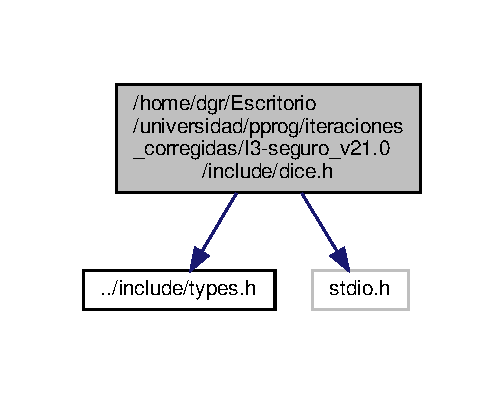
\includegraphics[width=236pt]{dice_8h__incl}
\end{center}
\end{figure}
This graph shows which files directly or indirectly include this file\+:\nopagebreak
\begin{figure}[H]
\begin{center}
\leavevmode
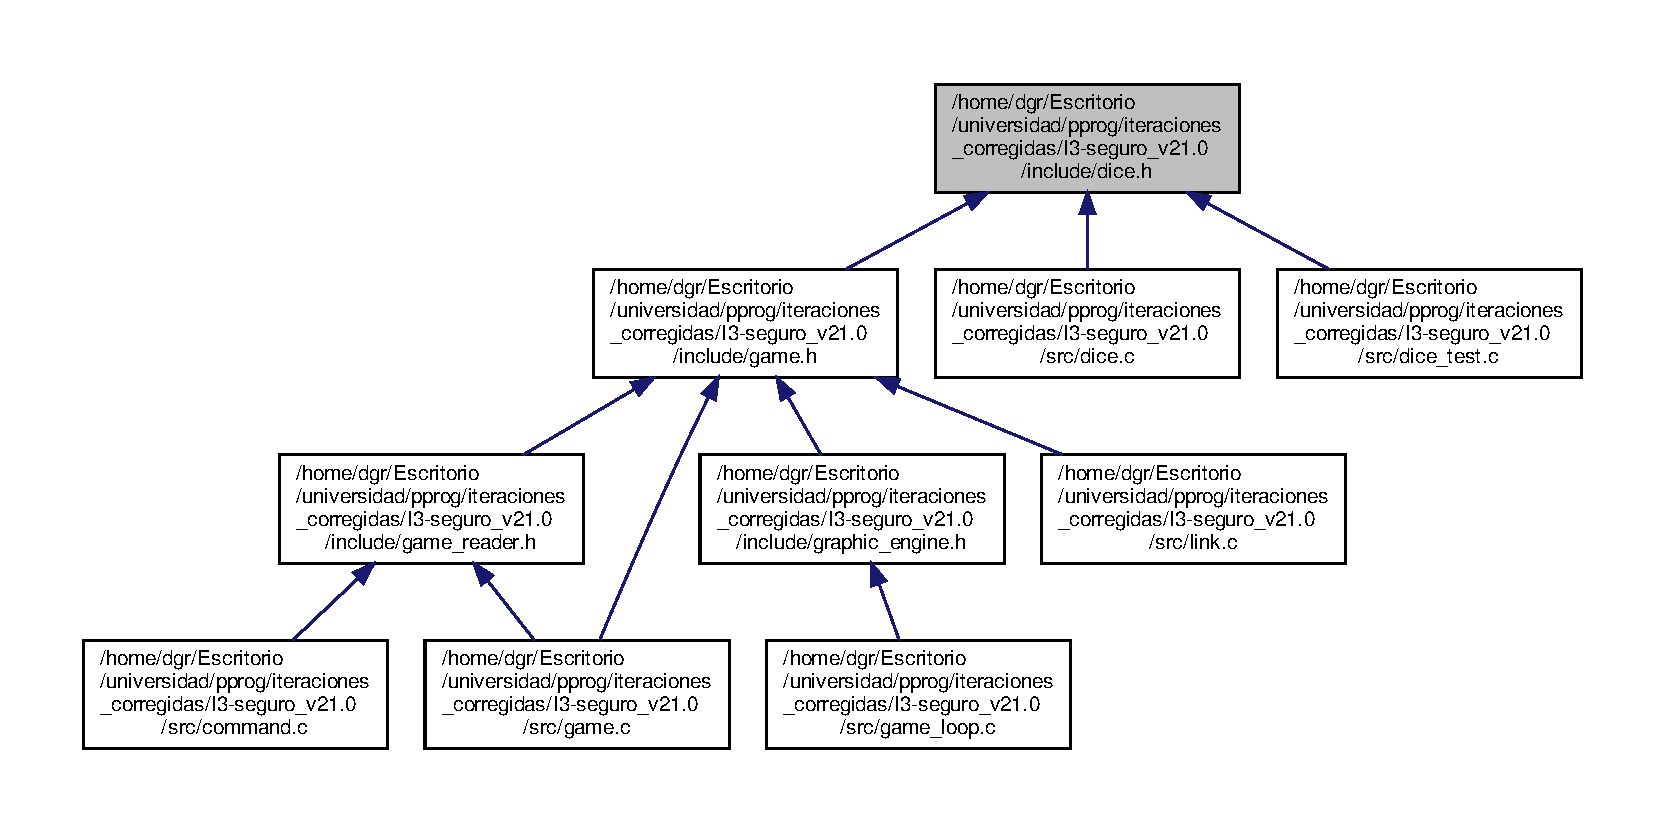
\includegraphics[width=350pt]{dice_8h__dep__incl}
\end{center}
\end{figure}
\subsection*{Typedefs}
\begin{DoxyCompactItemize}
\item 
typedef struct \hyperlink{struct__Dice}{\+\_\+\+Dice} \hyperlink{dice_8h_a5910ae86cf402855269700abd23e3976}{Dice}
\begin{DoxyCompactList}\small\item\em A type definition for a dice. \end{DoxyCompactList}\end{DoxyCompactItemize}
\subsection*{Functions}
\begin{DoxyCompactItemize}
\item 
\hyperlink{dice_8h_a5910ae86cf402855269700abd23e3976}{Dice} $\ast$ \hyperlink{dice_8h_a6f5f18873cfd3e4da81b40e33c7cf637}{dice\+\_\+create} (\hyperlink{types_8h_a845e604fb28f7e3d97549da3448149d3}{Id} id, int max, int min)
\begin{DoxyCompactList}\small\item\em Create a dice. \end{DoxyCompactList}\item 
\hyperlink{types_8h_a32c27cc471df37f4fc818d65de0a56c4}{S\+T\+A\+T\+US} \hyperlink{dice_8h_a2c673e593f984c182dc6dde3f6dcfd59}{dice\+\_\+destroy} (\hyperlink{dice_8h_a5910ae86cf402855269700abd23e3976}{Dice} $\ast$dice)
\begin{DoxyCompactList}\small\item\em free a dice \end{DoxyCompactList}\item 
int \hyperlink{dice_8h_ab1ad7da98578cf2db3c70daffccfb944}{dice\+\_\+roll} (\hyperlink{dice_8h_a5910ae86cf402855269700abd23e3976}{Dice} $\ast$dice)
\begin{DoxyCompactList}\small\item\em roll a dice \end{DoxyCompactList}\item 
\hyperlink{types_8h_a32c27cc471df37f4fc818d65de0a56c4}{S\+T\+A\+T\+US} \hyperlink{dice_8h_adc188c44ee8d1058c574f08ac39b5c6b}{dice\+\_\+print} (\hyperlink{dice_8h_a5910ae86cf402855269700abd23e3976}{Dice} $\ast$dice)
\begin{DoxyCompactList}\small\item\em print a dice \end{DoxyCompactList}\item 
int \hyperlink{dice_8h_a2bfe1653c086f66149ba8fc3f3b52017}{dice\+\_\+get\+\_\+last} (\hyperlink{dice_8h_a5910ae86cf402855269700abd23e3976}{Dice} $\ast$dice)
\begin{DoxyCompactList}\small\item\em get the last roll value \end{DoxyCompactList}\end{DoxyCompactItemize}


\subsection{Detailed Description}
It defines the dice interface for each command. 

\begin{DoxyAuthor}{Author}
David Teófilo Garitagoitia Romero 
\end{DoxyAuthor}
\begin{DoxyVersion}{Version}
1.\+0 
\end{DoxyVersion}
\begin{DoxyDate}{Date}
20-\/02-\/2020 
\end{DoxyDate}
\begin{DoxyCopyright}{Copyright}
G\+NU Public License 
\end{DoxyCopyright}


\subsection{Typedef Documentation}
\mbox{\Hypertarget{dice_8h_a5910ae86cf402855269700abd23e3976}\label{dice_8h_a5910ae86cf402855269700abd23e3976}} 
\index{dice.\+h@{dice.\+h}!Dice@{Dice}}
\index{Dice@{Dice}!dice.\+h@{dice.\+h}}
\subsubsection{\texorpdfstring{Dice}{Dice}}
{\footnotesize\ttfamily typedef struct \hyperlink{struct__Dice}{\+\_\+\+Dice} \hyperlink{dice_8h_a5910ae86cf402855269700abd23e3976}{Dice}}



A type definition for a dice. 

Details. 

\subsection{Function Documentation}
\mbox{\Hypertarget{dice_8h_a6f5f18873cfd3e4da81b40e33c7cf637}\label{dice_8h_a6f5f18873cfd3e4da81b40e33c7cf637}} 
\index{dice.\+h@{dice.\+h}!dice\+\_\+create@{dice\+\_\+create}}
\index{dice\+\_\+create@{dice\+\_\+create}!dice.\+h@{dice.\+h}}
\subsubsection{\texorpdfstring{dice\+\_\+create()}{dice\_create()}}
{\footnotesize\ttfamily \hyperlink{dice_8h_a5910ae86cf402855269700abd23e3976}{Dice}$\ast$ dice\+\_\+create (\begin{DoxyParamCaption}\item[{\hyperlink{types_8h_a845e604fb28f7e3d97549da3448149d3}{Id}}]{id,  }\item[{int}]{max,  }\item[{int}]{min }\end{DoxyParamCaption})}



Create a dice. 

dice\+\_\+create Create a dice with a specific Id, max and min

\begin{DoxyDate}{Date}
20-\/02-\/2019 
\end{DoxyDate}
\begin{DoxyAuthor}{Author}
David Teófilo Garitagoitia Romero
\end{DoxyAuthor}

\begin{DoxyParams}{Parameters}
{\em id} & the id of the new dice \\
\hline
{\em max} & the maximum of the dice \\
\hline
{\em min} & the minimum of the dice \\
\hline
\end{DoxyParams}
\begin{DoxyReturn}{Returns}
the new dice that has been created 
\end{DoxyReturn}
\mbox{\Hypertarget{dice_8h_a2c673e593f984c182dc6dde3f6dcfd59}\label{dice_8h_a2c673e593f984c182dc6dde3f6dcfd59}} 
\index{dice.\+h@{dice.\+h}!dice\+\_\+destroy@{dice\+\_\+destroy}}
\index{dice\+\_\+destroy@{dice\+\_\+destroy}!dice.\+h@{dice.\+h}}
\subsubsection{\texorpdfstring{dice\+\_\+destroy()}{dice\_destroy()}}
{\footnotesize\ttfamily \hyperlink{types_8h_a32c27cc471df37f4fc818d65de0a56c4}{S\+T\+A\+T\+US} dice\+\_\+destroy (\begin{DoxyParamCaption}\item[{\hyperlink{dice_8h_a5910ae86cf402855269700abd23e3976}{Dice} $\ast$}]{dice }\end{DoxyParamCaption})}



free a dice 

dice\+\_\+destroy free a especific dice

\begin{DoxyDate}{Date}
20-\/02-\/2019 
\end{DoxyDate}
\begin{DoxyAuthor}{Author}
David Teófilo Garitagoitia Romero
\end{DoxyAuthor}

\begin{DoxyParams}{Parameters}
{\em dice} & a dice that has been created before \\
\hline
\end{DoxyParams}
\begin{DoxyReturn}{Returns}
E\+R\+R\+OR if there is an error, otherwise return OK 
\end{DoxyReturn}
\mbox{\Hypertarget{dice_8h_a2bfe1653c086f66149ba8fc3f3b52017}\label{dice_8h_a2bfe1653c086f66149ba8fc3f3b52017}} 
\index{dice.\+h@{dice.\+h}!dice\+\_\+get\+\_\+last@{dice\+\_\+get\+\_\+last}}
\index{dice\+\_\+get\+\_\+last@{dice\+\_\+get\+\_\+last}!dice.\+h@{dice.\+h}}
\subsubsection{\texorpdfstring{dice\+\_\+get\+\_\+last()}{dice\_get\_last()}}
{\footnotesize\ttfamily int dice\+\_\+get\+\_\+last (\begin{DoxyParamCaption}\item[{\hyperlink{dice_8h_a5910ae86cf402855269700abd23e3976}{Dice} $\ast$}]{dice }\end{DoxyParamCaption})}



get the last roll value 

dice\+\_\+get\+\_\+last

\begin{DoxyDate}{Date}
20-\/02-\/2019 
\end{DoxyDate}
\begin{DoxyAuthor}{Author}
David Teófilo Garitagoitia Romero
\end{DoxyAuthor}

\begin{DoxyParams}{Parameters}
{\em dice} & a dice that has been created before \\
\hline
\end{DoxyParams}
\begin{DoxyReturn}{Returns}
-\/1 if there is an error, otherwise return the last roll value 
\end{DoxyReturn}
\mbox{\Hypertarget{dice_8h_adc188c44ee8d1058c574f08ac39b5c6b}\label{dice_8h_adc188c44ee8d1058c574f08ac39b5c6b}} 
\index{dice.\+h@{dice.\+h}!dice\+\_\+print@{dice\+\_\+print}}
\index{dice\+\_\+print@{dice\+\_\+print}!dice.\+h@{dice.\+h}}
\subsubsection{\texorpdfstring{dice\+\_\+print()}{dice\_print()}}
{\footnotesize\ttfamily \hyperlink{types_8h_a32c27cc471df37f4fc818d65de0a56c4}{S\+T\+A\+T\+US} dice\+\_\+print (\begin{DoxyParamCaption}\item[{\hyperlink{dice_8h_a5910ae86cf402855269700abd23e3976}{Dice} $\ast$}]{dice }\end{DoxyParamCaption})}



print a dice 

dice\+\_\+print print a especific dice

\begin{DoxyDate}{Date}
20-\/02-\/2019 
\end{DoxyDate}
\begin{DoxyAuthor}{Author}
David Teófilo Garitagoitia Romero
\end{DoxyAuthor}

\begin{DoxyParams}{Parameters}
{\em dice} & a dice which you want to print \\
\hline
\end{DoxyParams}
\begin{DoxyReturn}{Returns}
-\/1 if there is an error, otherwise return the number of the roll 
\end{DoxyReturn}
\mbox{\Hypertarget{dice_8h_ab1ad7da98578cf2db3c70daffccfb944}\label{dice_8h_ab1ad7da98578cf2db3c70daffccfb944}} 
\index{dice.\+h@{dice.\+h}!dice\+\_\+roll@{dice\+\_\+roll}}
\index{dice\+\_\+roll@{dice\+\_\+roll}!dice.\+h@{dice.\+h}}
\subsubsection{\texorpdfstring{dice\+\_\+roll()}{dice\_roll()}}
{\footnotesize\ttfamily int dice\+\_\+roll (\begin{DoxyParamCaption}\item[{\hyperlink{dice_8h_a5910ae86cf402855269700abd23e3976}{Dice} $\ast$}]{dice }\end{DoxyParamCaption})}



roll a dice 

dice\+\_\+roll roll a especific dice

\begin{DoxyDate}{Date}
20-\/02-\/2019 
\end{DoxyDate}
\begin{DoxyAuthor}{Author}
David Teófilo Garitagoitia Romero
\end{DoxyAuthor}

\begin{DoxyParams}{Parameters}
{\em dice} & a dice which you want to roll \\
\hline
\end{DoxyParams}
\begin{DoxyReturn}{Returns}
-\/1 if there is an error, otherwise return the number of the roll 
\end{DoxyReturn}

\hypertarget{dice__test_8h}{}\section{include/dice\+\_\+test.h File Reference}
\label{dice__test_8h}\index{include/dice\+\_\+test.\+h@{include/dice\+\_\+test.\+h}}


It declares the tests for the command module.  


This graph shows which files directly or indirectly include this file\+:\nopagebreak
\begin{figure}[H]
\begin{center}
\leavevmode
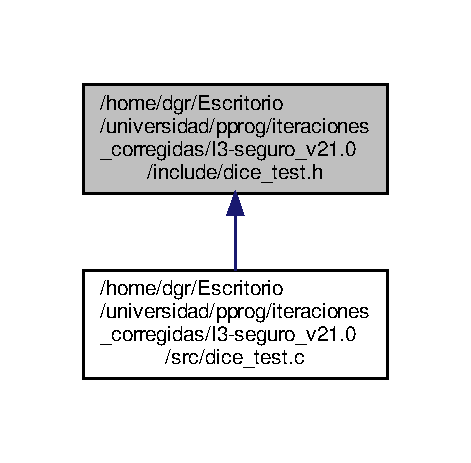
\includegraphics[width=178pt]{dice__test_8h__dep__incl}
\end{center}
\end{figure}
\subsection*{Functions}
\begin{DoxyCompactItemize}
\item 
void \hyperlink{dice__test_8h_afd8e7b7e3963ce0b48e40a7dcd4fb4b1}{test1\+\_\+dice\+\_\+create} ()
\item 
void \hyperlink{dice__test_8h_a3eacb7c8e4140ce2083d9705937f5106}{test2\+\_\+dice\+\_\+create} ()
\item 
void \hyperlink{dice__test_8h_a60f25d1250ef29f731d5e688fe989557}{test1\+\_\+dice\+\_\+roll} ()
\item 
void \hyperlink{dice__test_8h_a6c0509c7a5effe89212b9d786d9fc30c}{test2\+\_\+dice\+\_\+roll} ()
\item 
void \hyperlink{dice__test_8h_ab5b06d8e4cc2530d644b753d78a63314}{test3\+\_\+dice\+\_\+roll} ()
\item 
void \hyperlink{dice__test_8h_a3e678dfcb1adf09a85eb2e145088d053}{test1\+\_\+dice\+\_\+get\+\_\+last} ()
\item 
void \hyperlink{dice__test_8h_a5f15e643f69bfe582f6ffd548b92f846}{test2\+\_\+dice\+\_\+get\+\_\+last} ()
\item 
void \hyperlink{dice__test_8h_a80cc6894dcbee3feacca7da1b3cc82a3}{test3\+\_\+dice\+\_\+get\+\_\+last} ()
\item 
void \hyperlink{dice__test_8h_acfd69ccf21566f11ea0ccb8cc2f592ab}{test4\+\_\+dice\+\_\+get\+\_\+last} ()
\end{DoxyCompactItemize}


\subsection{Detailed Description}
It declares the tests for the command module. 

It declares the tests for the dice module.

\begin{DoxyAuthor}{Author}
David Teófilo Garitagoitia Romero 
\end{DoxyAuthor}
\begin{DoxyVersion}{Version}
1.\+0 
\end{DoxyVersion}
\begin{DoxyDate}{Date}
10-\/06-\/2020 
\end{DoxyDate}
\begin{DoxyCopyright}{Copyright}
G\+NU Public License
\end{DoxyCopyright}
\begin{DoxyAuthor}{Author}
Daniel Cerrato Sánchez 
\end{DoxyAuthor}
\begin{DoxyVersion}{Version}
1.\+0 
\end{DoxyVersion}
\begin{DoxyDate}{Date}
10-\/06-\/2020 
\end{DoxyDate}
\begin{DoxyCopyright}{Copyright}
G\+NU Public License 
\end{DoxyCopyright}


\subsection{Function Documentation}
\mbox{\Hypertarget{dice__test_8h_afd8e7b7e3963ce0b48e40a7dcd4fb4b1}\label{dice__test_8h_afd8e7b7e3963ce0b48e40a7dcd4fb4b1}} 
\index{dice\+\_\+test.\+h@{dice\+\_\+test.\+h}!test1\+\_\+dice\+\_\+create@{test1\+\_\+dice\+\_\+create}}
\index{test1\+\_\+dice\+\_\+create@{test1\+\_\+dice\+\_\+create}!dice\+\_\+test.\+h@{dice\+\_\+test.\+h}}
\subsubsection{\texorpdfstring{test1\+\_\+dice\+\_\+create()}{test1\_dice\_create()}}
{\footnotesize\ttfamily void test1\+\_\+dice\+\_\+create (\begin{DoxyParamCaption}{ }\end{DoxyParamCaption})}

\begin{DoxyRefDesc}{Test}
\item[\hyperlink{test__test000079}{Test}]Test the dice creation function \end{DoxyRefDesc}
\begin{DoxyPrecond}{Precondition}
An id, a maximum value and a minimum value in integer value as parameters, the maximum is greater than the minimum 
\end{DoxyPrecond}
\begin{DoxyPostcond}{Postcondition}
A non-\/null pointer to the created die 
\end{DoxyPostcond}
\mbox{\Hypertarget{dice__test_8h_a3e678dfcb1adf09a85eb2e145088d053}\label{dice__test_8h_a3e678dfcb1adf09a85eb2e145088d053}} 
\index{dice\+\_\+test.\+h@{dice\+\_\+test.\+h}!test1\+\_\+dice\+\_\+get\+\_\+last@{test1\+\_\+dice\+\_\+get\+\_\+last}}
\index{test1\+\_\+dice\+\_\+get\+\_\+last@{test1\+\_\+dice\+\_\+get\+\_\+last}!dice\+\_\+test.\+h@{dice\+\_\+test.\+h}}
\subsubsection{\texorpdfstring{test1\+\_\+dice\+\_\+get\+\_\+last()}{test1\_dice\_get\_last()}}
{\footnotesize\ttfamily void test1\+\_\+dice\+\_\+get\+\_\+last (\begin{DoxyParamCaption}{ }\end{DoxyParamCaption})}

\begin{DoxyRefDesc}{Test}
\item[\hyperlink{test__test000084}{Test}]Test the function to get the last value taken with the given \end{DoxyRefDesc}
\begin{DoxyPrecond}{Precondition}
The die is a non-\/\+N\+U\+LL pointer with the correct fields, after having thrown 
\end{DoxyPrecond}
\begin{DoxyPostcond}{Postcondition}
The output must be greater than or equal to the minimum value entered 
\end{DoxyPostcond}
\mbox{\Hypertarget{dice__test_8h_a60f25d1250ef29f731d5e688fe989557}\label{dice__test_8h_a60f25d1250ef29f731d5e688fe989557}} 
\index{dice\+\_\+test.\+h@{dice\+\_\+test.\+h}!test1\+\_\+dice\+\_\+roll@{test1\+\_\+dice\+\_\+roll}}
\index{test1\+\_\+dice\+\_\+roll@{test1\+\_\+dice\+\_\+roll}!dice\+\_\+test.\+h@{dice\+\_\+test.\+h}}
\subsubsection{\texorpdfstring{test1\+\_\+dice\+\_\+roll()}{test1\_dice\_roll()}}
{\footnotesize\ttfamily void test1\+\_\+dice\+\_\+roll (\begin{DoxyParamCaption}{ }\end{DoxyParamCaption})}

\begin{DoxyRefDesc}{Test}
\item[\hyperlink{test__test000081}{Test}]Test the function to get a value from the dice \end{DoxyRefDesc}
\begin{DoxyPrecond}{Precondition}
The die is a non-\/\+N\+U\+LL pointer with the correct fields 
\end{DoxyPrecond}
\begin{DoxyPostcond}{Postcondition}
The output must be greater than or equal to the minimum value entered 
\end{DoxyPostcond}
\mbox{\Hypertarget{dice__test_8h_a3eacb7c8e4140ce2083d9705937f5106}\label{dice__test_8h_a3eacb7c8e4140ce2083d9705937f5106}} 
\index{dice\+\_\+test.\+h@{dice\+\_\+test.\+h}!test2\+\_\+dice\+\_\+create@{test2\+\_\+dice\+\_\+create}}
\index{test2\+\_\+dice\+\_\+create@{test2\+\_\+dice\+\_\+create}!dice\+\_\+test.\+h@{dice\+\_\+test.\+h}}
\subsubsection{\texorpdfstring{test2\+\_\+dice\+\_\+create()}{test2\_dice\_create()}}
{\footnotesize\ttfamily void test2\+\_\+dice\+\_\+create (\begin{DoxyParamCaption}{ }\end{DoxyParamCaption})}

\begin{DoxyRefDesc}{Test}
\item[\hyperlink{test__test000080}{Test}]Test the dice creation function \end{DoxyRefDesc}
\begin{DoxyPrecond}{Precondition}
An id, a maximum value and a minimum value in integer value as parameters, the minimum is greater than the maximum 
\end{DoxyPrecond}
\begin{DoxyPostcond}{Postcondition}
A null pointer to the created die 
\end{DoxyPostcond}
\mbox{\Hypertarget{dice__test_8h_a5f15e643f69bfe582f6ffd548b92f846}\label{dice__test_8h_a5f15e643f69bfe582f6ffd548b92f846}} 
\index{dice\+\_\+test.\+h@{dice\+\_\+test.\+h}!test2\+\_\+dice\+\_\+get\+\_\+last@{test2\+\_\+dice\+\_\+get\+\_\+last}}
\index{test2\+\_\+dice\+\_\+get\+\_\+last@{test2\+\_\+dice\+\_\+get\+\_\+last}!dice\+\_\+test.\+h@{dice\+\_\+test.\+h}}
\subsubsection{\texorpdfstring{test2\+\_\+dice\+\_\+get\+\_\+last()}{test2\_dice\_get\_last()}}
{\footnotesize\ttfamily void test2\+\_\+dice\+\_\+get\+\_\+last (\begin{DoxyParamCaption}{ }\end{DoxyParamCaption})}

\begin{DoxyRefDesc}{Test}
\item[\hyperlink{test__test000085}{Test}]Test the function to get the last value taken with the given \end{DoxyRefDesc}
\begin{DoxyPrecond}{Precondition}
The die is a non-\/\+N\+U\+LL pointer with the correct fields, after having thrown 
\end{DoxyPrecond}
\begin{DoxyPostcond}{Postcondition}
The output must be less than or equal to the maximum value entered 
\end{DoxyPostcond}
\mbox{\Hypertarget{dice__test_8h_a6c0509c7a5effe89212b9d786d9fc30c}\label{dice__test_8h_a6c0509c7a5effe89212b9d786d9fc30c}} 
\index{dice\+\_\+test.\+h@{dice\+\_\+test.\+h}!test2\+\_\+dice\+\_\+roll@{test2\+\_\+dice\+\_\+roll}}
\index{test2\+\_\+dice\+\_\+roll@{test2\+\_\+dice\+\_\+roll}!dice\+\_\+test.\+h@{dice\+\_\+test.\+h}}
\subsubsection{\texorpdfstring{test2\+\_\+dice\+\_\+roll()}{test2\_dice\_roll()}}
{\footnotesize\ttfamily void test2\+\_\+dice\+\_\+roll (\begin{DoxyParamCaption}{ }\end{DoxyParamCaption})}

\begin{DoxyRefDesc}{Test}
\item[\hyperlink{test__test000082}{Test}]Test the function to get a value from the dice \end{DoxyRefDesc}
\begin{DoxyPrecond}{Precondition}
The die is a non-\/\+N\+U\+LL pointer with the correct fields 
\end{DoxyPrecond}
\begin{DoxyPostcond}{Postcondition}
The output must be less than or equal to the maximum value entered 
\end{DoxyPostcond}
\mbox{\Hypertarget{dice__test_8h_a80cc6894dcbee3feacca7da1b3cc82a3}\label{dice__test_8h_a80cc6894dcbee3feacca7da1b3cc82a3}} 
\index{dice\+\_\+test.\+h@{dice\+\_\+test.\+h}!test3\+\_\+dice\+\_\+get\+\_\+last@{test3\+\_\+dice\+\_\+get\+\_\+last}}
\index{test3\+\_\+dice\+\_\+get\+\_\+last@{test3\+\_\+dice\+\_\+get\+\_\+last}!dice\+\_\+test.\+h@{dice\+\_\+test.\+h}}
\subsubsection{\texorpdfstring{test3\+\_\+dice\+\_\+get\+\_\+last()}{test3\_dice\_get\_last()}}
{\footnotesize\ttfamily void test3\+\_\+dice\+\_\+get\+\_\+last (\begin{DoxyParamCaption}{ }\end{DoxyParamCaption})}

\begin{DoxyRefDesc}{Test}
\item[\hyperlink{test__test000086}{Test}]Test the function to get the last value taken with the given \end{DoxyRefDesc}
\begin{DoxyPrecond}{Precondition}
The die is a non-\/\+N\+U\+LL pointer with the correct fields, without having thrown 
\end{DoxyPrecond}
\begin{DoxyPostcond}{Postcondition}
The output must be 0 
\end{DoxyPostcond}
\mbox{\Hypertarget{dice__test_8h_ab5b06d8e4cc2530d644b753d78a63314}\label{dice__test_8h_ab5b06d8e4cc2530d644b753d78a63314}} 
\index{dice\+\_\+test.\+h@{dice\+\_\+test.\+h}!test3\+\_\+dice\+\_\+roll@{test3\+\_\+dice\+\_\+roll}}
\index{test3\+\_\+dice\+\_\+roll@{test3\+\_\+dice\+\_\+roll}!dice\+\_\+test.\+h@{dice\+\_\+test.\+h}}
\subsubsection{\texorpdfstring{test3\+\_\+dice\+\_\+roll()}{test3\_dice\_roll()}}
{\footnotesize\ttfamily void test3\+\_\+dice\+\_\+roll (\begin{DoxyParamCaption}{ }\end{DoxyParamCaption})}

\begin{DoxyRefDesc}{Test}
\item[\hyperlink{test__test000083}{Test}]Test the function to get a value from the dice \end{DoxyRefDesc}
\begin{DoxyPrecond}{Precondition}
The die is a pointer to N\+U\+LL 
\end{DoxyPrecond}
\begin{DoxyPostcond}{Postcondition}
The output must be -\/1 
\end{DoxyPostcond}
\mbox{\Hypertarget{dice__test_8h_acfd69ccf21566f11ea0ccb8cc2f592ab}\label{dice__test_8h_acfd69ccf21566f11ea0ccb8cc2f592ab}} 
\index{dice\+\_\+test.\+h@{dice\+\_\+test.\+h}!test4\+\_\+dice\+\_\+get\+\_\+last@{test4\+\_\+dice\+\_\+get\+\_\+last}}
\index{test4\+\_\+dice\+\_\+get\+\_\+last@{test4\+\_\+dice\+\_\+get\+\_\+last}!dice\+\_\+test.\+h@{dice\+\_\+test.\+h}}
\subsubsection{\texorpdfstring{test4\+\_\+dice\+\_\+get\+\_\+last()}{test4\_dice\_get\_last()}}
{\footnotesize\ttfamily void test4\+\_\+dice\+\_\+get\+\_\+last (\begin{DoxyParamCaption}{ }\end{DoxyParamCaption})}

\begin{DoxyRefDesc}{Test}
\item[\hyperlink{test__test000087}{Test}]Test the function to get the last value taken with the given \end{DoxyRefDesc}
\begin{DoxyPrecond}{Precondition}
The die is a pointer to N\+U\+LL 
\end{DoxyPrecond}
\begin{DoxyPostcond}{Postcondition}
The output must be -\/1 
\end{DoxyPostcond}

\hypertarget{game_8h}{}\section{/home/dgr/\+Escritorio/universidad/pprog/iteraciones\+\_\+corregidas/\+I3-\/seguro\+\_\+v21.0/include/game.h File Reference}
\label{game_8h}\index{/home/dgr/\+Escritorio/universidad/pprog/iteraciones\+\_\+corregidas/\+I3-\/seguro\+\_\+v21.\+0/include/game.\+h@{/home/dgr/\+Escritorio/universidad/pprog/iteraciones\+\_\+corregidas/\+I3-\/seguro\+\_\+v21.\+0/include/game.\+h}}


It defines the game interface for each command.  


{\ttfamily \#include \char`\"{}../include/command.\+h\char`\"{}}\newline
{\ttfamily \#include \char`\"{}../include/space.\+h\char`\"{}}\newline
{\ttfamily \#include \char`\"{}../include/player.\+h\char`\"{}}\newline
{\ttfamily \#include \char`\"{}../include/object.\+h\char`\"{}}\newline
{\ttfamily \#include \char`\"{}../include/dice.\+h\char`\"{}}\newline
{\ttfamily \#include \char`\"{}../include/link.\+h\char`\"{}}\newline
Include dependency graph for game.\+h\+:
\nopagebreak
\begin{figure}[H]
\begin{center}
\leavevmode
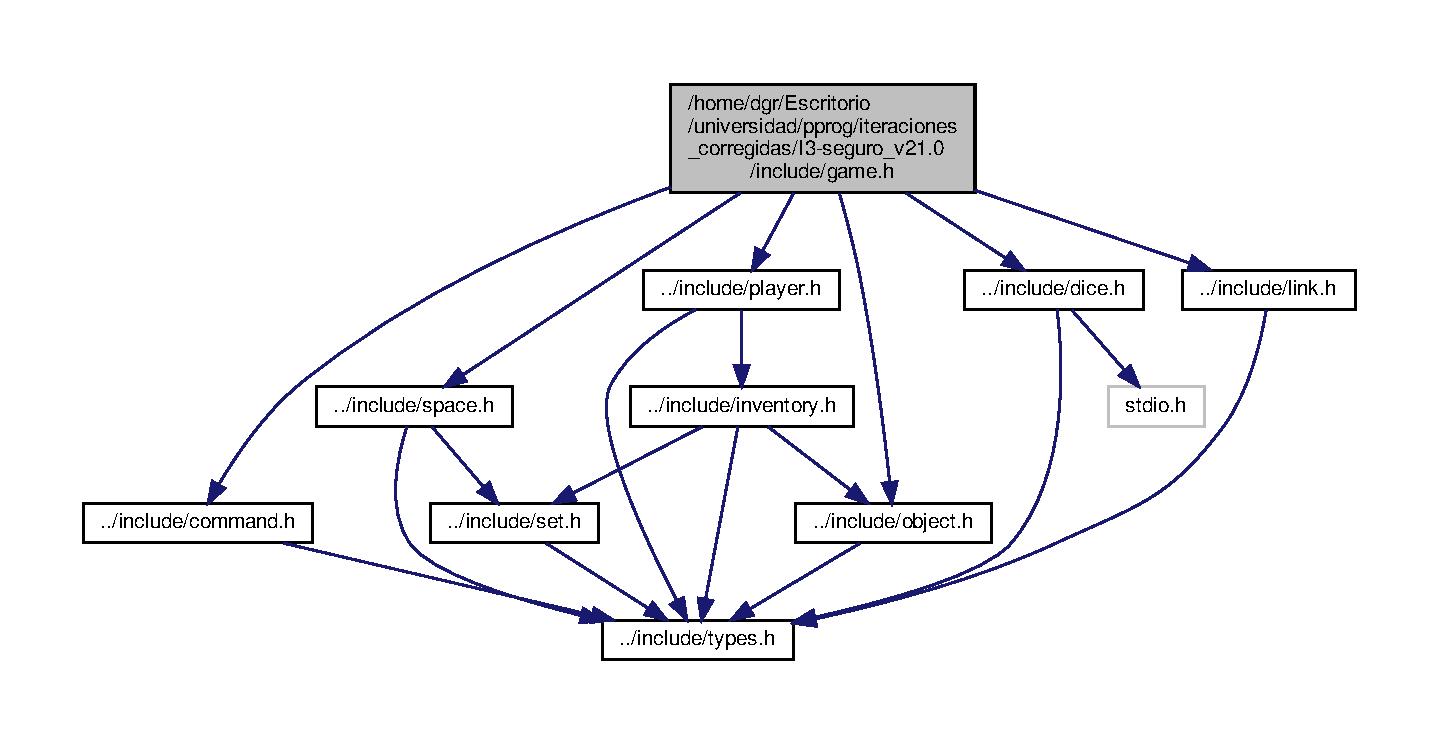
\includegraphics[width=350pt]{game_8h__incl}
\end{center}
\end{figure}
This graph shows which files directly or indirectly include this file\+:
\nopagebreak
\begin{figure}[H]
\begin{center}
\leavevmode
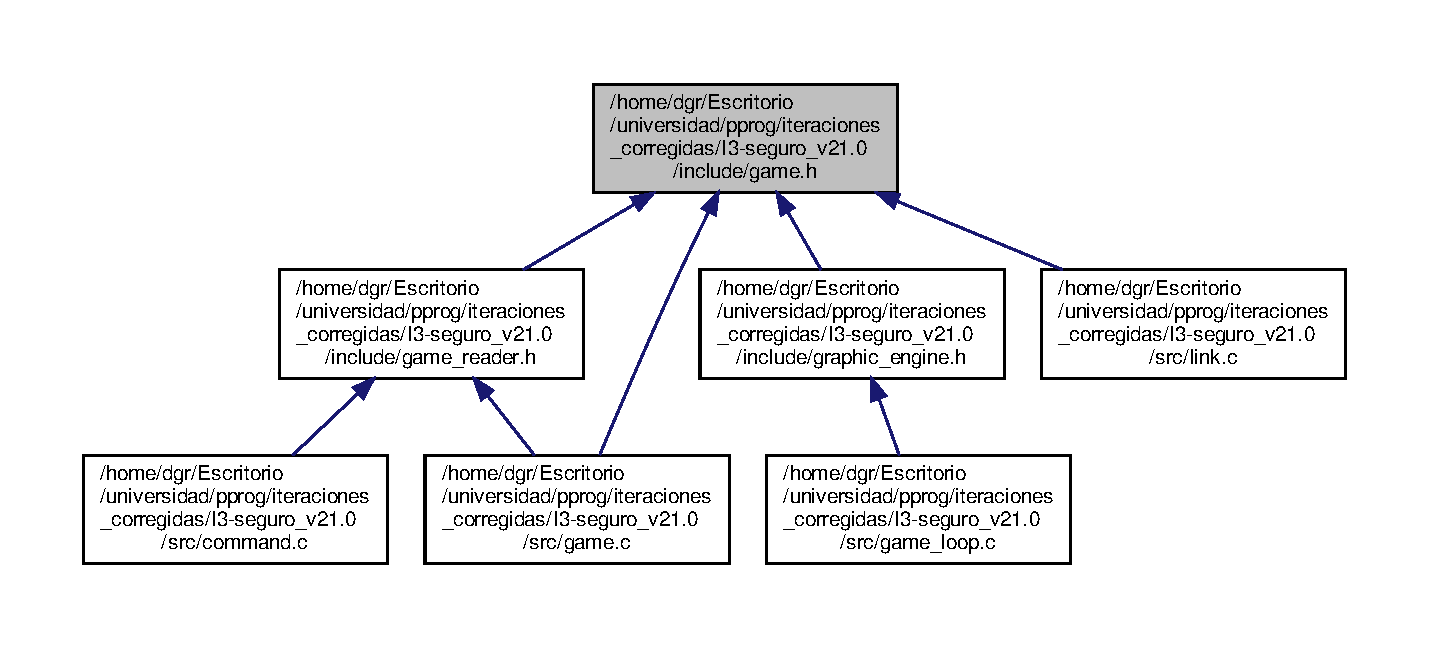
\includegraphics[width=350pt]{game_8h__dep__incl}
\end{center}
\end{figure}
\subsection*{Macros}
\begin{DoxyCompactItemize}
\item 
\#define \hyperlink{game_8h_acdc7844fbd4d45737d4aa56834d37829}{M\+A\+X\+\_\+\+O\+B\+J\+E\+C\+TS}~10
\begin{DoxyCompactList}\small\item\em A macro that stores the maximum objects of a game. \end{DoxyCompactList}\item 
\#define \hyperlink{game_8h_a660ed1ec8604982002a0d6eced0e0367}{M\+A\+X\+\_\+\+L\+I\+N\+KS}~400
\begin{DoxyCompactList}\small\item\em A macro that stores the maximum links of a game. \end{DoxyCompactList}\end{DoxyCompactItemize}
\subsection*{Typedefs}
\begin{DoxyCompactItemize}
\item 
typedef struct \hyperlink{struct__Game}{\+\_\+\+Game} \hyperlink{game_8h_a57156d39c530aec3fba3a9dad8c2dc6a}{Game}
\begin{DoxyCompactList}\small\item\em A type definition for a game. \end{DoxyCompactList}\end{DoxyCompactItemize}
\subsection*{Functions}
\begin{DoxyCompactItemize}
\item 
\hyperlink{game_8h_a57156d39c530aec3fba3a9dad8c2dc6a}{Game} $\ast$ \hyperlink{game_8h_a1cdbe3f06b9bf49eb5e334a22ad3b2b9}{game\+\_\+create} ()
\begin{DoxyCompactList}\small\item\em Create the game, initialite the variables of the game. \end{DoxyCompactList}\item 
\hyperlink{game_8h_a57156d39c530aec3fba3a9dad8c2dc6a}{Game} $\ast$ \hyperlink{game_8h_a0e225eaf98598147fdfba6fed2ea8f02}{game\+\_\+create\+\_\+from\+\_\+file} (char $\ast$filename)
\begin{DoxyCompactList}\small\item\em Create the game from a file. \end{DoxyCompactList}\item 
\hyperlink{types_8h_a32c27cc471df37f4fc818d65de0a56c4}{S\+T\+A\+T\+US} \hyperlink{game_8h_a8711cf50c2cef44e064da433807e252a}{game\+\_\+update} (\hyperlink{game_8h_a57156d39c530aec3fba3a9dad8c2dc6a}{Game} $\ast$game, \hyperlink{command_8h_a0473597db8c45c0289b6b8e2f8abbe32}{T\+\_\+\+Command} command, char $\ast$argument)
\begin{DoxyCompactList}\small\item\em update the game \end{DoxyCompactList}\item 
\hyperlink{types_8h_a32c27cc471df37f4fc818d65de0a56c4}{S\+T\+A\+T\+US} \hyperlink{game_8h_a0736924a1235c0e6fe9b6d91c2a12af8}{game\+\_\+destroy} (\hyperlink{game_8h_a57156d39c530aec3fba3a9dad8c2dc6a}{Game} $\ast$game)
\begin{DoxyCompactList}\small\item\em free the game \end{DoxyCompactList}\item 
\hyperlink{types_8h_a3e5b8192e7d9ffaf3542f1210aec18dd}{B\+O\+OL} \hyperlink{game_8h_aa6efe0650af110bbd84e742cc8046d93}{game\+\_\+is\+\_\+over} (\hyperlink{game_8h_a57156d39c530aec3fba3a9dad8c2dc6a}{Game} $\ast$game)
\begin{DoxyCompactList}\small\item\em check if the game is over \end{DoxyCompactList}\item 
void \hyperlink{game_8h_a33a5ed8937423f8c012df3cedad4fa4c}{game\+\_\+print\+\_\+data} (\hyperlink{game_8h_a57156d39c530aec3fba3a9dad8c2dc6a}{Game} $\ast$game)
\begin{DoxyCompactList}\small\item\em print the game data \end{DoxyCompactList}\item 
\hyperlink{space_8h_a67533ffc2b70463baecc38fb0629bbfc}{Space} $\ast$ \hyperlink{game_8h_a69d94da9d27b542d3ebdeb8b60f1f2dc}{game\+\_\+get\+\_\+space} (\hyperlink{game_8h_a57156d39c530aec3fba3a9dad8c2dc6a}{Game} $\ast$game, \hyperlink{types_8h_a845e604fb28f7e3d97549da3448149d3}{Id} id)
\begin{DoxyCompactList}\small\item\em get the space \end{DoxyCompactList}\item 
\hyperlink{command_8h_a0473597db8c45c0289b6b8e2f8abbe32}{T\+\_\+\+Command} \hyperlink{game_8h_ac6c33f046d4854d4357ca95428a41281}{game\+\_\+get\+\_\+last\+\_\+principal\+\_\+command} (\hyperlink{game_8h_a57156d39c530aec3fba3a9dad8c2dc6a}{Game} $\ast$game)
\begin{DoxyCompactList}\small\item\em get the last command of the game \end{DoxyCompactList}\item 
\hyperlink{types_8h_a32c27cc471df37f4fc818d65de0a56c4}{S\+T\+A\+T\+US} \hyperlink{game_8h_ae5ad86de0a92d9eccb234948458da7f1}{game\+\_\+add\+\_\+space} (\hyperlink{game_8h_a57156d39c530aec3fba3a9dad8c2dc6a}{Game} $\ast$game, \hyperlink{space_8h_a67533ffc2b70463baecc38fb0629bbfc}{Space} $\ast$space)
\begin{DoxyCompactList}\small\item\em add a space in the game \end{DoxyCompactList}\item 
\hyperlink{types_8h_a845e604fb28f7e3d97549da3448149d3}{Id} \hyperlink{game_8h_a83b86a040470f67786d912f45efc9eb8}{game\+\_\+get\+\_\+object\+\_\+location} (\hyperlink{game_8h_a57156d39c530aec3fba3a9dad8c2dc6a}{Game} $\ast$game, \hyperlink{types_8h_a845e604fb28f7e3d97549da3448149d3}{Id} object)
\begin{DoxyCompactList}\small\item\em get the location of an object \end{DoxyCompactList}\item 
\hyperlink{types_8h_a845e604fb28f7e3d97549da3448149d3}{Id} \hyperlink{game_8h_ad2dfd865e2bd2c545a15d33f4d1cf3ae}{game\+\_\+get\+\_\+space\+\_\+id\+\_\+at} (\hyperlink{game_8h_a57156d39c530aec3fba3a9dad8c2dc6a}{Game} $\ast$game, int position)
\begin{DoxyCompactList}\small\item\em return the id of an space form their position \end{DoxyCompactList}\item 
\hyperlink{types_8h_a32c27cc471df37f4fc818d65de0a56c4}{S\+T\+A\+T\+US} \hyperlink{game_8h_a9597a8e456aa74db536e87d56f56c3b4}{game\+\_\+add\+\_\+object} (\hyperlink{game_8h_a57156d39c530aec3fba3a9dad8c2dc6a}{Game} $\ast$game, \hyperlink{object_8h_a7f8bbcda919b65ce67f92fba08e0212f}{Object} $\ast$object)
\begin{DoxyCompactList}\small\item\em add a new object to the game \end{DoxyCompactList}\item 
const char $\ast$ \hyperlink{game_8h_a2ecf68dd442c912c2b0da3c3dd9fef9e}{game\+\_\+get\+\_\+object\+\_\+name\+\_\+at\+\_\+id} (\hyperlink{game_8h_a57156d39c530aec3fba3a9dad8c2dc6a}{Game} $\ast$game, \hyperlink{types_8h_a845e604fb28f7e3d97549da3448149d3}{Id} id)
\begin{DoxyCompactList}\small\item\em return the name of an object from his id \end{DoxyCompactList}\item 
void \hyperlink{game_8h_a81ff7aff49ff47a7a16a88df4ae06956}{game\+\_\+get\+\_\+objects\+\_\+name\+\_\+at\+\_\+space} (\hyperlink{space_8h_a67533ffc2b70463baecc38fb0629bbfc}{Space} $\ast$space, \hyperlink{game_8h_a57156d39c530aec3fba3a9dad8c2dc6a}{Game} $\ast$game, char $\ast$names)
\begin{DoxyCompactList}\small\item\em save a string with the name of all objects of an space in the names argument \end{DoxyCompactList}\item 
void \hyperlink{game_8h_ab6154c70ef6dd43b0dc7089d6f363974}{game\+\_\+get\+\_\+objects\+\_\+location} (\hyperlink{game_8h_a57156d39c530aec3fba3a9dad8c2dc6a}{Game} $\ast$game, char $\ast$names)
\begin{DoxyCompactList}\small\item\em save a string with the name of all objects of the game and their locations in the names argument \end{DoxyCompactList}\item 
char $\ast$ \hyperlink{game_8h_a89c667c3db1a1afe426c264a742d373c}{game\+\_\+get\+\_\+last\+\_\+argument} (\hyperlink{game_8h_a57156d39c530aec3fba3a9dad8c2dc6a}{Game} $\ast$game)
\begin{DoxyCompactList}\small\item\em get the argument insert by the user \end{DoxyCompactList}\item 
\hyperlink{command_8h_a7d2935971c252377cb0fc1c8545dc2bc}{Command} $\ast$ \hyperlink{game_8h_a0622ea04a0e30e49f51ed4c83257bee5}{game\+\_\+get\+\_\+last\+\_\+command} (\hyperlink{game_8h_a57156d39c530aec3fba3a9dad8c2dc6a}{Game} $\ast$game)
\begin{DoxyCompactList}\small\item\em get the comand insert by the user \end{DoxyCompactList}\item 
\hyperlink{player_8h_af30e2030635a69690f85e48bc6ef202f}{Player} $\ast$ \hyperlink{game_8h_af46efd507d797aec6da90d08aa592e32}{game\+\_\+get\+\_\+player} (\hyperlink{game_8h_a57156d39c530aec3fba3a9dad8c2dc6a}{Game} $\ast$game)
\begin{DoxyCompactList}\small\item\em get the player of the game \end{DoxyCompactList}\item 
\hyperlink{dice_8h_a5910ae86cf402855269700abd23e3976}{Dice} $\ast$ \hyperlink{game_8h_ab32e231181826f82db6c6d161d2eb647}{game\+\_\+get\+\_\+dice} (\hyperlink{game_8h_a57156d39c530aec3fba3a9dad8c2dc6a}{Game} $\ast$game)
\begin{DoxyCompactList}\small\item\em get the dice of the game \end{DoxyCompactList}\item 
void \hyperlink{game_8h_ab13626a54ff51e2300a82f5c6ebd6ec7}{game\+\_\+get\+\_\+player\+\_\+objects} (\hyperlink{game_8h_a57156d39c530aec3fba3a9dad8c2dc6a}{Game} $\ast$game, char $\ast$names)
\begin{DoxyCompactList}\small\item\em get the player objects of the game \end{DoxyCompactList}\item 
\hyperlink{types_8h_a32c27cc471df37f4fc818d65de0a56c4}{S\+T\+A\+T\+US} \hyperlink{game_8h_ade0d25f267771b1f9b27fcc0383e93b8}{game\+\_\+set\+\_\+player} (\hyperlink{game_8h_a57156d39c530aec3fba3a9dad8c2dc6a}{Game} $\ast$game, \hyperlink{player_8h_af30e2030635a69690f85e48bc6ef202f}{Player} $\ast$player)
\begin{DoxyCompactList}\small\item\em set the player of the game \end{DoxyCompactList}\item 
\hyperlink{types_8h_a32c27cc471df37f4fc818d65de0a56c4}{S\+T\+A\+T\+US} \hyperlink{game_8h_a4691bee17d5784ad6eb257dfbb252c27}{game\+\_\+add\+\_\+link} (\hyperlink{game_8h_a57156d39c530aec3fba3a9dad8c2dc6a}{Game} $\ast$game, \hyperlink{link_8h_ae3b299941e67be6971bfd64a25505eff}{Link} $\ast$link)
\begin{DoxyCompactList}\small\item\em add a link to the game \end{DoxyCompactList}\item 
\hyperlink{link_8h_ae3b299941e67be6971bfd64a25505eff}{Link} $\ast$ \hyperlink{game_8h_a34824b782ef05dcca98e83546b321ebf}{game\+\_\+get\+\_\+link\+\_\+at\+\_\+id} (\hyperlink{game_8h_a57156d39c530aec3fba3a9dad8c2dc6a}{Game} $\ast$game, \hyperlink{types_8h_a845e604fb28f7e3d97549da3448149d3}{Id} id)
\begin{DoxyCompactList}\small\item\em return a link pointer from their id \end{DoxyCompactList}\item 
\hyperlink{types_8h_a845e604fb28f7e3d97549da3448149d3}{Id} \hyperlink{game_8h_ab08e136689431b2c932cfcac2131c51a}{game\+\_\+get\+\_\+south} (\hyperlink{game_8h_a57156d39c530aec3fba3a9dad8c2dc6a}{Game} $\ast$game, \hyperlink{space_8h_a67533ffc2b70463baecc38fb0629bbfc}{Space} $\ast$space)
\begin{DoxyCompactList}\small\item\em returns the id of the souther link of the space \end{DoxyCompactList}\item 
\hyperlink{types_8h_a845e604fb28f7e3d97549da3448149d3}{Id} \hyperlink{game_8h_a19a5cd5f4230efccff68d10af5af40e8}{game\+\_\+get\+\_\+north} (\hyperlink{game_8h_a57156d39c530aec3fba3a9dad8c2dc6a}{Game} $\ast$game, \hyperlink{space_8h_a67533ffc2b70463baecc38fb0629bbfc}{Space} $\ast$space)
\begin{DoxyCompactList}\small\item\em returns the id of the north link of the space \end{DoxyCompactList}\item 
\hyperlink{types_8h_a845e604fb28f7e3d97549da3448149d3}{Id} \hyperlink{game_8h_a23b7636aa7306962aaf1358697cabd76}{game\+\_\+get\+\_\+east} (\hyperlink{game_8h_a57156d39c530aec3fba3a9dad8c2dc6a}{Game} $\ast$game, \hyperlink{space_8h_a67533ffc2b70463baecc38fb0629bbfc}{Space} $\ast$space)
\begin{DoxyCompactList}\small\item\em returns the id of the east link of the space \end{DoxyCompactList}\item 
\hyperlink{types_8h_a845e604fb28f7e3d97549da3448149d3}{Id} \hyperlink{game_8h_ad86395a448cc3e6100cdcef36427d840}{game\+\_\+get\+\_\+west} (\hyperlink{game_8h_a57156d39c530aec3fba3a9dad8c2dc6a}{Game} $\ast$game, \hyperlink{space_8h_a67533ffc2b70463baecc38fb0629bbfc}{Space} $\ast$space)
\begin{DoxyCompactList}\small\item\em returns the id of the west link of the space \end{DoxyCompactList}\end{DoxyCompactItemize}


\subsection{Detailed Description}
It defines the game interface for each command. 

\begin{DoxyAuthor}{Author}
Profesores P\+P\+R\+OG, David Garitagoitia Romero y José Manuel García Giráldez 
\end{DoxyAuthor}
\begin{DoxyVersion}{Version}
1.\+0 
\end{DoxyVersion}
\begin{DoxyDate}{Date}
13-\/01-\/2015 
\end{DoxyDate}
\begin{DoxyCopyright}{Copyright}
G\+NU Public License 
\end{DoxyCopyright}


\subsection{Macro Definition Documentation}
\mbox{\Hypertarget{game_8h_a660ed1ec8604982002a0d6eced0e0367}\label{game_8h_a660ed1ec8604982002a0d6eced0e0367}} 
\index{game.\+h@{game.\+h}!M\+A\+X\+\_\+\+L\+I\+N\+KS@{M\+A\+X\+\_\+\+L\+I\+N\+KS}}
\index{M\+A\+X\+\_\+\+L\+I\+N\+KS@{M\+A\+X\+\_\+\+L\+I\+N\+KS}!game.\+h@{game.\+h}}
\subsubsection{\texorpdfstring{M\+A\+X\+\_\+\+L\+I\+N\+KS}{MAX\_LINKS}}
{\footnotesize\ttfamily \#define M\+A\+X\+\_\+\+L\+I\+N\+KS~400}



A macro that stores the maximum links of a game. 

Details. \mbox{\Hypertarget{game_8h_acdc7844fbd4d45737d4aa56834d37829}\label{game_8h_acdc7844fbd4d45737d4aa56834d37829}} 
\index{game.\+h@{game.\+h}!M\+A\+X\+\_\+\+O\+B\+J\+E\+C\+TS@{M\+A\+X\+\_\+\+O\+B\+J\+E\+C\+TS}}
\index{M\+A\+X\+\_\+\+O\+B\+J\+E\+C\+TS@{M\+A\+X\+\_\+\+O\+B\+J\+E\+C\+TS}!game.\+h@{game.\+h}}
\subsubsection{\texorpdfstring{M\+A\+X\+\_\+\+O\+B\+J\+E\+C\+TS}{MAX\_OBJECTS}}
{\footnotesize\ttfamily \#define M\+A\+X\+\_\+\+O\+B\+J\+E\+C\+TS~10}



A macro that stores the maximum objects of a game. 

Details. 

\subsection{Typedef Documentation}
\mbox{\Hypertarget{game_8h_a57156d39c530aec3fba3a9dad8c2dc6a}\label{game_8h_a57156d39c530aec3fba3a9dad8c2dc6a}} 
\index{game.\+h@{game.\+h}!Game@{Game}}
\index{Game@{Game}!game.\+h@{game.\+h}}
\subsubsection{\texorpdfstring{Game}{Game}}
{\footnotesize\ttfamily typedef struct \hyperlink{struct__Game}{\+\_\+\+Game} \hyperlink{game_8h_a57156d39c530aec3fba3a9dad8c2dc6a}{Game}}



A type definition for a game. 

Details. 

\subsection{Function Documentation}
\mbox{\Hypertarget{game_8h_a4691bee17d5784ad6eb257dfbb252c27}\label{game_8h_a4691bee17d5784ad6eb257dfbb252c27}} 
\index{game.\+h@{game.\+h}!game\+\_\+add\+\_\+link@{game\+\_\+add\+\_\+link}}
\index{game\+\_\+add\+\_\+link@{game\+\_\+add\+\_\+link}!game.\+h@{game.\+h}}
\subsubsection{\texorpdfstring{game\+\_\+add\+\_\+link()}{game\_add\_link()}}
{\footnotesize\ttfamily \hyperlink{types_8h_a32c27cc471df37f4fc818d65de0a56c4}{S\+T\+A\+T\+US} game\+\_\+add\+\_\+link (\begin{DoxyParamCaption}\item[{\hyperlink{game_8h_a57156d39c530aec3fba3a9dad8c2dc6a}{Game} $\ast$}]{game,  }\item[{\hyperlink{link_8h_ae3b299941e67be6971bfd64a25505eff}{Link} $\ast$}]{link }\end{DoxyParamCaption})}



add a link to the game 

game\+\_\+add\+\_\+link

\begin{DoxyDate}{Date}
13-\/03-\/2020 
\end{DoxyDate}
\begin{DoxyAuthor}{Author}
David Teófilo Garitagoitia Romero
\end{DoxyAuthor}

\begin{DoxyParams}{Parameters}
{\em game} & the strcture game we initialite \\
\hline
{\em link} & the link that we want to add to the game \\
\hline
\end{DoxyParams}
\begin{DoxyReturn}{Returns}
Ok if there is no error, E\+R\+R\+OR otherwise 
\end{DoxyReturn}
\mbox{\Hypertarget{game_8h_a9597a8e456aa74db536e87d56f56c3b4}\label{game_8h_a9597a8e456aa74db536e87d56f56c3b4}} 
\index{game.\+h@{game.\+h}!game\+\_\+add\+\_\+object@{game\+\_\+add\+\_\+object}}
\index{game\+\_\+add\+\_\+object@{game\+\_\+add\+\_\+object}!game.\+h@{game.\+h}}
\subsubsection{\texorpdfstring{game\+\_\+add\+\_\+object()}{game\_add\_object()}}
{\footnotesize\ttfamily \hyperlink{types_8h_a32c27cc471df37f4fc818d65de0a56c4}{S\+T\+A\+T\+US} game\+\_\+add\+\_\+object (\begin{DoxyParamCaption}\item[{\hyperlink{game_8h_a57156d39c530aec3fba3a9dad8c2dc6a}{Game} $\ast$}]{game,  }\item[{\hyperlink{object_8h_a7f8bbcda919b65ce67f92fba08e0212f}{Object} $\ast$}]{object }\end{DoxyParamCaption})}



add a new object to the game 

game\+\_\+add\+\_\+object

\begin{DoxyDate}{Date}
01-\/03-\/2020 
\end{DoxyDate}
\begin{DoxyAuthor}{Author}
\+: David Teófilo Garitagoitia Romero
\end{DoxyAuthor}

\begin{DoxyParams}{Parameters}
{\em game} & the strcture game we initialite \\
\hline
{\em object} & the addres to the object that we want to add \\
\hline
\end{DoxyParams}
\begin{DoxyReturn}{Returns}
E\+R\+R\+OR if there is an error, otherwise return OK 
\end{DoxyReturn}
\mbox{\Hypertarget{game_8h_ae5ad86de0a92d9eccb234948458da7f1}\label{game_8h_ae5ad86de0a92d9eccb234948458da7f1}} 
\index{game.\+h@{game.\+h}!game\+\_\+add\+\_\+space@{game\+\_\+add\+\_\+space}}
\index{game\+\_\+add\+\_\+space@{game\+\_\+add\+\_\+space}!game.\+h@{game.\+h}}
\subsubsection{\texorpdfstring{game\+\_\+add\+\_\+space()}{game\_add\_space()}}
{\footnotesize\ttfamily \hyperlink{types_8h_a32c27cc471df37f4fc818d65de0a56c4}{S\+T\+A\+T\+US} game\+\_\+add\+\_\+space (\begin{DoxyParamCaption}\item[{\hyperlink{game_8h_a57156d39c530aec3fba3a9dad8c2dc6a}{Game} $\ast$}]{game,  }\item[{\hyperlink{space_8h_a67533ffc2b70463baecc38fb0629bbfc}{Space} $\ast$}]{space }\end{DoxyParamCaption})}



add a space in the game 

game\+\_\+add\+\_\+space

\begin{DoxyDate}{Date}
13-\/01-\/2015 
\end{DoxyDate}
\begin{DoxyAuthor}{Author}
\+: Instructors of P\+P\+R\+OG
\end{DoxyAuthor}

\begin{DoxyParams}{Parameters}
{\em game} & the game in which we will add the space \\
\hline
{\em space} & the space which will be add in the game \\
\hline
\end{DoxyParams}
\begin{DoxyReturn}{Returns}
E\+R\+R\+OR if there is an error, otherwise return OK 
\end{DoxyReturn}
\mbox{\Hypertarget{game_8h_a1cdbe3f06b9bf49eb5e334a22ad3b2b9}\label{game_8h_a1cdbe3f06b9bf49eb5e334a22ad3b2b9}} 
\index{game.\+h@{game.\+h}!game\+\_\+create@{game\+\_\+create}}
\index{game\+\_\+create@{game\+\_\+create}!game.\+h@{game.\+h}}
\subsubsection{\texorpdfstring{game\+\_\+create()}{game\_create()}}
{\footnotesize\ttfamily \hyperlink{game_8h_a57156d39c530aec3fba3a9dad8c2dc6a}{Game}$\ast$ game\+\_\+create (\begin{DoxyParamCaption}{ }\end{DoxyParamCaption})}



Create the game, initialite the variables of the game. 

Game interface implementation game\+\_\+create

\begin{DoxyDate}{Date}
13-\/01-\/2015 
\end{DoxyDate}
\begin{DoxyAuthor}{Author}
\+: Instructors of P\+P\+R\+OG
\end{DoxyAuthor}
\begin{DoxyReturn}{Returns}
the game created 
\end{DoxyReturn}
\mbox{\Hypertarget{game_8h_a0e225eaf98598147fdfba6fed2ea8f02}\label{game_8h_a0e225eaf98598147fdfba6fed2ea8f02}} 
\index{game.\+h@{game.\+h}!game\+\_\+create\+\_\+from\+\_\+file@{game\+\_\+create\+\_\+from\+\_\+file}}
\index{game\+\_\+create\+\_\+from\+\_\+file@{game\+\_\+create\+\_\+from\+\_\+file}!game.\+h@{game.\+h}}
\subsubsection{\texorpdfstring{game\+\_\+create\+\_\+from\+\_\+file()}{game\_create\_from\_file()}}
{\footnotesize\ttfamily \hyperlink{game_8h_a57156d39c530aec3fba3a9dad8c2dc6a}{Game}$\ast$ game\+\_\+create\+\_\+from\+\_\+file (\begin{DoxyParamCaption}\item[{char $\ast$}]{filename }\end{DoxyParamCaption})}



Create the game from a file. 

game\+\_\+create\+\_\+from\+\_\+file

\begin{DoxyDate}{Date}
13-\/01-\/2015 
\end{DoxyDate}
\begin{DoxyAuthor}{Author}
\+: Instructors of P\+P\+R\+OG
\end{DoxyAuthor}

\begin{DoxyParams}{Parameters}
{\em filename} & the name of the file we will use \\
\hline
\end{DoxyParams}
\begin{DoxyReturn}{Returns}
E\+R\+R\+OR if there is an error, otherwise return OK 
\end{DoxyReturn}
\mbox{\Hypertarget{game_8h_a0736924a1235c0e6fe9b6d91c2a12af8}\label{game_8h_a0736924a1235c0e6fe9b6d91c2a12af8}} 
\index{game.\+h@{game.\+h}!game\+\_\+destroy@{game\+\_\+destroy}}
\index{game\+\_\+destroy@{game\+\_\+destroy}!game.\+h@{game.\+h}}
\subsubsection{\texorpdfstring{game\+\_\+destroy()}{game\_destroy()}}
{\footnotesize\ttfamily \hyperlink{types_8h_a32c27cc471df37f4fc818d65de0a56c4}{S\+T\+A\+T\+US} game\+\_\+destroy (\begin{DoxyParamCaption}\item[{\hyperlink{game_8h_a57156d39c530aec3fba3a9dad8c2dc6a}{Game} $\ast$}]{game }\end{DoxyParamCaption})}



free the game 

game\+\_\+destroy

\begin{DoxyDate}{Date}
13-\/01-\/2015 
\end{DoxyDate}
\begin{DoxyAuthor}{Author}
\+: Instructors of P\+P\+R\+OG
\end{DoxyAuthor}

\begin{DoxyParams}{Parameters}
{\em game} & a game that has been created before \\
\hline
\end{DoxyParams}
\begin{DoxyReturn}{Returns}
E\+R\+R\+OR if there is an error, otherwise return OK 
\end{DoxyReturn}
\mbox{\Hypertarget{game_8h_ab32e231181826f82db6c6d161d2eb647}\label{game_8h_ab32e231181826f82db6c6d161d2eb647}} 
\index{game.\+h@{game.\+h}!game\+\_\+get\+\_\+dice@{game\+\_\+get\+\_\+dice}}
\index{game\+\_\+get\+\_\+dice@{game\+\_\+get\+\_\+dice}!game.\+h@{game.\+h}}
\subsubsection{\texorpdfstring{game\+\_\+get\+\_\+dice()}{game\_get\_dice()}}
{\footnotesize\ttfamily \hyperlink{dice_8h_a5910ae86cf402855269700abd23e3976}{Dice}$\ast$ game\+\_\+get\+\_\+dice (\begin{DoxyParamCaption}\item[{\hyperlink{game_8h_a57156d39c530aec3fba3a9dad8c2dc6a}{Game} $\ast$}]{game }\end{DoxyParamCaption})}



get the dice of the game 

game\+\_\+get\+\_\+player

\begin{DoxyDate}{Date}
13-\/03-\/2020 
\end{DoxyDate}
\begin{DoxyAuthor}{Author}
David Teófilo Garitagoitia Romero
\end{DoxyAuthor}

\begin{DoxyParams}{Parameters}
{\em game} & the strcture game we initialite \\
\hline
\end{DoxyParams}
\begin{DoxyReturn}{Returns}
the addres of the dice 
\end{DoxyReturn}
\mbox{\Hypertarget{game_8h_a23b7636aa7306962aaf1358697cabd76}\label{game_8h_a23b7636aa7306962aaf1358697cabd76}} 
\index{game.\+h@{game.\+h}!game\+\_\+get\+\_\+east@{game\+\_\+get\+\_\+east}}
\index{game\+\_\+get\+\_\+east@{game\+\_\+get\+\_\+east}!game.\+h@{game.\+h}}
\subsubsection{\texorpdfstring{game\+\_\+get\+\_\+east()}{game\_get\_east()}}
{\footnotesize\ttfamily \hyperlink{types_8h_a845e604fb28f7e3d97549da3448149d3}{Id} game\+\_\+get\+\_\+east (\begin{DoxyParamCaption}\item[{\hyperlink{game_8h_a57156d39c530aec3fba3a9dad8c2dc6a}{Game} $\ast$}]{game,  }\item[{\hyperlink{space_8h_a67533ffc2b70463baecc38fb0629bbfc}{Space} $\ast$}]{space }\end{DoxyParamCaption})}



returns the id of the east link of the space 

game\+\_\+get\+\_\+east

\begin{DoxyDate}{Date}
13-\/03-\/2020 
\end{DoxyDate}
\begin{DoxyAuthor}{Author}
David Teófilo Garitagoitia Romero
\end{DoxyAuthor}

\begin{DoxyParams}{Parameters}
{\em game} & the strcture game we initialite \\
\hline
{\em space} & the space we want to know about its east link \\
\hline
\end{DoxyParams}
\begin{DoxyReturn}{Returns}
the id of the east link of the space 
\end{DoxyReturn}
\mbox{\Hypertarget{game_8h_a89c667c3db1a1afe426c264a742d373c}\label{game_8h_a89c667c3db1a1afe426c264a742d373c}} 
\index{game.\+h@{game.\+h}!game\+\_\+get\+\_\+last\+\_\+argument@{game\+\_\+get\+\_\+last\+\_\+argument}}
\index{game\+\_\+get\+\_\+last\+\_\+argument@{game\+\_\+get\+\_\+last\+\_\+argument}!game.\+h@{game.\+h}}
\subsubsection{\texorpdfstring{game\+\_\+get\+\_\+last\+\_\+argument()}{game\_get\_last\_argument()}}
{\footnotesize\ttfamily char$\ast$ game\+\_\+get\+\_\+last\+\_\+argument (\begin{DoxyParamCaption}\item[{\hyperlink{game_8h_a57156d39c530aec3fba3a9dad8c2dc6a}{Game} $\ast$}]{game }\end{DoxyParamCaption})}



get the argument insert by the user 

game\+\_\+get\+\_\+last\+\_\+argument

\begin{DoxyDate}{Date}
05-\/03-\/2020 
\end{DoxyDate}
\begin{DoxyAuthor}{Author}
José Manuel García Giráldez
\end{DoxyAuthor}

\begin{DoxyParams}{Parameters}
{\em game} & the strcture game we initialite \\
\hline
\end{DoxyParams}
\begin{DoxyReturn}{Returns}
the argument 
\end{DoxyReturn}
\mbox{\Hypertarget{game_8h_a0622ea04a0e30e49f51ed4c83257bee5}\label{game_8h_a0622ea04a0e30e49f51ed4c83257bee5}} 
\index{game.\+h@{game.\+h}!game\+\_\+get\+\_\+last\+\_\+command@{game\+\_\+get\+\_\+last\+\_\+command}}
\index{game\+\_\+get\+\_\+last\+\_\+command@{game\+\_\+get\+\_\+last\+\_\+command}!game.\+h@{game.\+h}}
\subsubsection{\texorpdfstring{game\+\_\+get\+\_\+last\+\_\+command()}{game\_get\_last\_command()}}
{\footnotesize\ttfamily \hyperlink{command_8h_a7d2935971c252377cb0fc1c8545dc2bc}{Command}$\ast$ game\+\_\+get\+\_\+last\+\_\+command (\begin{DoxyParamCaption}\item[{\hyperlink{game_8h_a57156d39c530aec3fba3a9dad8c2dc6a}{Game} $\ast$}]{game }\end{DoxyParamCaption})}



get the comand insert by the user 

game\+\_\+get\+\_\+last\+\_\+command

\begin{DoxyDate}{Date}
02-\/03-\/2020 
\end{DoxyDate}
\begin{DoxyAuthor}{Author}
David Teófilo Garitagoitia Romero
\end{DoxyAuthor}

\begin{DoxyParams}{Parameters}
{\em game} & the strcture game we initialite \\
\hline
\end{DoxyParams}
\begin{DoxyReturn}{Returns}
the command 
\end{DoxyReturn}
\mbox{\Hypertarget{game_8h_ac6c33f046d4854d4357ca95428a41281}\label{game_8h_ac6c33f046d4854d4357ca95428a41281}} 
\index{game.\+h@{game.\+h}!game\+\_\+get\+\_\+last\+\_\+principal\+\_\+command@{game\+\_\+get\+\_\+last\+\_\+principal\+\_\+command}}
\index{game\+\_\+get\+\_\+last\+\_\+principal\+\_\+command@{game\+\_\+get\+\_\+last\+\_\+principal\+\_\+command}!game.\+h@{game.\+h}}
\subsubsection{\texorpdfstring{game\+\_\+get\+\_\+last\+\_\+principal\+\_\+command()}{game\_get\_last\_principal\_command()}}
{\footnotesize\ttfamily \hyperlink{command_8h_a0473597db8c45c0289b6b8e2f8abbe32}{T\+\_\+\+Command} game\+\_\+get\+\_\+last\+\_\+principal\+\_\+command (\begin{DoxyParamCaption}\item[{\hyperlink{game_8h_a57156d39c530aec3fba3a9dad8c2dc6a}{Game} $\ast$}]{game }\end{DoxyParamCaption})}



get the last command of the game 

game\+\_\+get\+\_\+last\+\_\+principal\+\_\+command

\begin{DoxyDate}{Date}
13-\/01-\/2015 
\end{DoxyDate}
\begin{DoxyAuthor}{Author}
\+: Instructors of P\+P\+R\+OG
\end{DoxyAuthor}

\begin{DoxyParams}{Parameters}
{\em game} & the game from which we will get the information \\
\hline
\end{DoxyParams}
\begin{DoxyReturn}{Returns}
game-\/$>$last\+\_\+cmd the last command 
\end{DoxyReturn}
\mbox{\Hypertarget{game_8h_a34824b782ef05dcca98e83546b321ebf}\label{game_8h_a34824b782ef05dcca98e83546b321ebf}} 
\index{game.\+h@{game.\+h}!game\+\_\+get\+\_\+link\+\_\+at\+\_\+id@{game\+\_\+get\+\_\+link\+\_\+at\+\_\+id}}
\index{game\+\_\+get\+\_\+link\+\_\+at\+\_\+id@{game\+\_\+get\+\_\+link\+\_\+at\+\_\+id}!game.\+h@{game.\+h}}
\subsubsection{\texorpdfstring{game\+\_\+get\+\_\+link\+\_\+at\+\_\+id()}{game\_get\_link\_at\_id()}}
{\footnotesize\ttfamily \hyperlink{link_8h_ae3b299941e67be6971bfd64a25505eff}{Link}$\ast$ game\+\_\+get\+\_\+link\+\_\+at\+\_\+id (\begin{DoxyParamCaption}\item[{\hyperlink{game_8h_a57156d39c530aec3fba3a9dad8c2dc6a}{Game} $\ast$}]{game,  }\item[{\hyperlink{types_8h_a845e604fb28f7e3d97549da3448149d3}{Id}}]{id }\end{DoxyParamCaption})}



return a link pointer from their id 

game\+\_\+get\+\_\+link\+\_\+at\+\_\+id

\begin{DoxyDate}{Date}
13-\/03-\/2020 
\end{DoxyDate}
\begin{DoxyAuthor}{Author}
David Teófilo Garitagoitia Romero
\end{DoxyAuthor}

\begin{DoxyParams}{Parameters}
{\em game} & the strcture game we initialite \\
\hline
{\em id} & the id of the link we want to get \\
\hline
\end{DoxyParams}
\begin{DoxyReturn}{Returns}
a pointer to the link that have that id 
\end{DoxyReturn}
\mbox{\Hypertarget{game_8h_a19a5cd5f4230efccff68d10af5af40e8}\label{game_8h_a19a5cd5f4230efccff68d10af5af40e8}} 
\index{game.\+h@{game.\+h}!game\+\_\+get\+\_\+north@{game\+\_\+get\+\_\+north}}
\index{game\+\_\+get\+\_\+north@{game\+\_\+get\+\_\+north}!game.\+h@{game.\+h}}
\subsubsection{\texorpdfstring{game\+\_\+get\+\_\+north()}{game\_get\_north()}}
{\footnotesize\ttfamily \hyperlink{types_8h_a845e604fb28f7e3d97549da3448149d3}{Id} game\+\_\+get\+\_\+north (\begin{DoxyParamCaption}\item[{\hyperlink{game_8h_a57156d39c530aec3fba3a9dad8c2dc6a}{Game} $\ast$}]{game,  }\item[{\hyperlink{space_8h_a67533ffc2b70463baecc38fb0629bbfc}{Space} $\ast$}]{space }\end{DoxyParamCaption})}



returns the id of the north link of the space 

game\+\_\+get\+\_\+north

\begin{DoxyDate}{Date}
13-\/03-\/2020 
\end{DoxyDate}
\begin{DoxyAuthor}{Author}
David Teófilo Garitagoitia Romero
\end{DoxyAuthor}

\begin{DoxyParams}{Parameters}
{\em game} & the strcture game we initialite \\
\hline
{\em space} & the space we want to know about its north link \\
\hline
\end{DoxyParams}
\begin{DoxyReturn}{Returns}
the id of the north link of the space 
\end{DoxyReturn}
\mbox{\Hypertarget{game_8h_a83b86a040470f67786d912f45efc9eb8}\label{game_8h_a83b86a040470f67786d912f45efc9eb8}} 
\index{game.\+h@{game.\+h}!game\+\_\+get\+\_\+object\+\_\+location@{game\+\_\+get\+\_\+object\+\_\+location}}
\index{game\+\_\+get\+\_\+object\+\_\+location@{game\+\_\+get\+\_\+object\+\_\+location}!game.\+h@{game.\+h}}
\subsubsection{\texorpdfstring{game\+\_\+get\+\_\+object\+\_\+location()}{game\_get\_object\_location()}}
{\footnotesize\ttfamily \hyperlink{types_8h_a845e604fb28f7e3d97549da3448149d3}{Id} game\+\_\+get\+\_\+object\+\_\+location (\begin{DoxyParamCaption}\item[{\hyperlink{game_8h_a57156d39c530aec3fba3a9dad8c2dc6a}{Game} $\ast$}]{game,  }\item[{\hyperlink{types_8h_a845e604fb28f7e3d97549da3448149d3}{Id}}]{object }\end{DoxyParamCaption})}



get the location of an object 

game\+\_\+get\+\_\+object\+\_\+location

\begin{DoxyDate}{Date}
09-\/02-\/2020 
\end{DoxyDate}
\begin{DoxyAuthor}{Author}
David Garitagoitia Romero
\end{DoxyAuthor}

\begin{DoxyParams}{Parameters}
{\em game} & the strcture game we initialite \\
\hline
{\em object} & the object which we want to know the id \\
\hline
\end{DoxyParams}
\begin{DoxyReturn}{Returns}
space\+\_\+get\+\_\+id(game-\/$>$spaces\mbox{[}i\mbox{]}) the id of the object 
\end{DoxyReturn}
\mbox{\Hypertarget{game_8h_a2ecf68dd442c912c2b0da3c3dd9fef9e}\label{game_8h_a2ecf68dd442c912c2b0da3c3dd9fef9e}} 
\index{game.\+h@{game.\+h}!game\+\_\+get\+\_\+object\+\_\+name\+\_\+at\+\_\+id@{game\+\_\+get\+\_\+object\+\_\+name\+\_\+at\+\_\+id}}
\index{game\+\_\+get\+\_\+object\+\_\+name\+\_\+at\+\_\+id@{game\+\_\+get\+\_\+object\+\_\+name\+\_\+at\+\_\+id}!game.\+h@{game.\+h}}
\subsubsection{\texorpdfstring{game\+\_\+get\+\_\+object\+\_\+name\+\_\+at\+\_\+id()}{game\_get\_object\_name\_at\_id()}}
{\footnotesize\ttfamily const char$\ast$ game\+\_\+get\+\_\+object\+\_\+name\+\_\+at\+\_\+id (\begin{DoxyParamCaption}\item[{\hyperlink{game_8h_a57156d39c530aec3fba3a9dad8c2dc6a}{Game} $\ast$}]{game,  }\item[{\hyperlink{types_8h_a845e604fb28f7e3d97549da3448149d3}{Id}}]{id }\end{DoxyParamCaption})}



return the name of an object from his id 

game\+\_\+get\+\_\+object\+\_\+name\+\_\+at\+\_\+id

\begin{DoxyDate}{Date}
01-\/03-\/2020 
\end{DoxyDate}
\begin{DoxyAuthor}{Author}
\+: David Teófilo Garitagoitia Romero
\end{DoxyAuthor}

\begin{DoxyParams}{Parameters}
{\em game} & the strcture game we initialite \\
\hline
{\em id} & the id of the object that we want to know his name \\
\hline
\end{DoxyParams}
\begin{DoxyReturn}{Returns}
N\+U\+LL if there is an error, otherwise return the name 
\end{DoxyReturn}
\mbox{\Hypertarget{game_8h_ab6154c70ef6dd43b0dc7089d6f363974}\label{game_8h_ab6154c70ef6dd43b0dc7089d6f363974}} 
\index{game.\+h@{game.\+h}!game\+\_\+get\+\_\+objects\+\_\+location@{game\+\_\+get\+\_\+objects\+\_\+location}}
\index{game\+\_\+get\+\_\+objects\+\_\+location@{game\+\_\+get\+\_\+objects\+\_\+location}!game.\+h@{game.\+h}}
\subsubsection{\texorpdfstring{game\+\_\+get\+\_\+objects\+\_\+location()}{game\_get\_objects\_location()}}
{\footnotesize\ttfamily void game\+\_\+get\+\_\+objects\+\_\+location (\begin{DoxyParamCaption}\item[{\hyperlink{game_8h_a57156d39c530aec3fba3a9dad8c2dc6a}{Game} $\ast$}]{game,  }\item[{char $\ast$}]{names }\end{DoxyParamCaption})}



save a string with the name of all objects of the game and their locations in the names argument 

game\+\_\+get\+\_\+objects\+\_\+location

\begin{DoxyDate}{Date}
01-\/03-\/2020 
\end{DoxyDate}
\begin{DoxyAuthor}{Author}
\+: David Teófilo Garitagoitia Romero
\end{DoxyAuthor}

\begin{DoxyParams}{Parameters}
{\em game} & the strcture game we initialite \\
\hline
{\em names} & the addres of an string in which the names of the objects and their location will be allocated \\
\hline
\end{DoxyParams}
\begin{DoxyReturn}{Returns}

\end{DoxyReturn}
\mbox{\Hypertarget{game_8h_a81ff7aff49ff47a7a16a88df4ae06956}\label{game_8h_a81ff7aff49ff47a7a16a88df4ae06956}} 
\index{game.\+h@{game.\+h}!game\+\_\+get\+\_\+objects\+\_\+name\+\_\+at\+\_\+space@{game\+\_\+get\+\_\+objects\+\_\+name\+\_\+at\+\_\+space}}
\index{game\+\_\+get\+\_\+objects\+\_\+name\+\_\+at\+\_\+space@{game\+\_\+get\+\_\+objects\+\_\+name\+\_\+at\+\_\+space}!game.\+h@{game.\+h}}
\subsubsection{\texorpdfstring{game\+\_\+get\+\_\+objects\+\_\+name\+\_\+at\+\_\+space()}{game\_get\_objects\_name\_at\_space()}}
{\footnotesize\ttfamily void game\+\_\+get\+\_\+objects\+\_\+name\+\_\+at\+\_\+space (\begin{DoxyParamCaption}\item[{\hyperlink{space_8h_a67533ffc2b70463baecc38fb0629bbfc}{Space} $\ast$}]{space,  }\item[{\hyperlink{game_8h_a57156d39c530aec3fba3a9dad8c2dc6a}{Game} $\ast$}]{game,  }\item[{char $\ast$}]{names }\end{DoxyParamCaption})}



save a string with the name of all objects of an space in the names argument 

game\+\_\+get\+\_\+object\+\_\+name\+\_\+at\+\_\+space

\begin{DoxyDate}{Date}
01-\/03-\/2020 
\end{DoxyDate}
\begin{DoxyAuthor}{Author}
\+: David Teófilo Garitagoitia Romero
\end{DoxyAuthor}

\begin{DoxyParams}{Parameters}
{\em space} & the space that you want to recive their objects name \\
\hline
{\em game} & the strcture game we initialite \\
\hline
{\em names} & the addres of an string in which the names will be allocated \\
\hline
\end{DoxyParams}
\begin{DoxyReturn}{Returns}

\end{DoxyReturn}
\mbox{\Hypertarget{game_8h_af46efd507d797aec6da90d08aa592e32}\label{game_8h_af46efd507d797aec6da90d08aa592e32}} 
\index{game.\+h@{game.\+h}!game\+\_\+get\+\_\+player@{game\+\_\+get\+\_\+player}}
\index{game\+\_\+get\+\_\+player@{game\+\_\+get\+\_\+player}!game.\+h@{game.\+h}}
\subsubsection{\texorpdfstring{game\+\_\+get\+\_\+player()}{game\_get\_player()}}
{\footnotesize\ttfamily \hyperlink{player_8h_af30e2030635a69690f85e48bc6ef202f}{Player}$\ast$ game\+\_\+get\+\_\+player (\begin{DoxyParamCaption}\item[{\hyperlink{game_8h_a57156d39c530aec3fba3a9dad8c2dc6a}{Game} $\ast$}]{game }\end{DoxyParamCaption})}



get the player of the game 

game\+\_\+get\+\_\+player

\begin{DoxyDate}{Date}
14-\/03-\/2020 
\end{DoxyDate}
\begin{DoxyAuthor}{Author}
David Teófilo Garitagoitia Romero
\end{DoxyAuthor}

\begin{DoxyParams}{Parameters}
{\em game} & the strcture game we initialite \\
\hline
\end{DoxyParams}
\begin{DoxyReturn}{Returns}
the addres of the player 
\end{DoxyReturn}
\mbox{\Hypertarget{game_8h_ab13626a54ff51e2300a82f5c6ebd6ec7}\label{game_8h_ab13626a54ff51e2300a82f5c6ebd6ec7}} 
\index{game.\+h@{game.\+h}!game\+\_\+get\+\_\+player\+\_\+objects@{game\+\_\+get\+\_\+player\+\_\+objects}}
\index{game\+\_\+get\+\_\+player\+\_\+objects@{game\+\_\+get\+\_\+player\+\_\+objects}!game.\+h@{game.\+h}}
\subsubsection{\texorpdfstring{game\+\_\+get\+\_\+player\+\_\+objects()}{game\_get\_player\_objects()}}
{\footnotesize\ttfamily void game\+\_\+get\+\_\+player\+\_\+objects (\begin{DoxyParamCaption}\item[{\hyperlink{game_8h_a57156d39c530aec3fba3a9dad8c2dc6a}{Game} $\ast$}]{game,  }\item[{char $\ast$}]{names }\end{DoxyParamCaption})}



get the player objects of the game 

game\+\_\+get\+\_\+player\+\_\+objects

\begin{DoxyDate}{Date}
13-\/03-\/2020 
\end{DoxyDate}
\begin{DoxyAuthor}{Author}
David Teófilo Garitagoitia Romero
\end{DoxyAuthor}

\begin{DoxyParams}{Parameters}
{\em game} & the strcture game we initialite \\
\hline
{\em names} & the string in which the objects will be written \\
\hline
\end{DoxyParams}
\mbox{\Hypertarget{game_8h_ab08e136689431b2c932cfcac2131c51a}\label{game_8h_ab08e136689431b2c932cfcac2131c51a}} 
\index{game.\+h@{game.\+h}!game\+\_\+get\+\_\+south@{game\+\_\+get\+\_\+south}}
\index{game\+\_\+get\+\_\+south@{game\+\_\+get\+\_\+south}!game.\+h@{game.\+h}}
\subsubsection{\texorpdfstring{game\+\_\+get\+\_\+south()}{game\_get\_south()}}
{\footnotesize\ttfamily \hyperlink{types_8h_a845e604fb28f7e3d97549da3448149d3}{Id} game\+\_\+get\+\_\+south (\begin{DoxyParamCaption}\item[{\hyperlink{game_8h_a57156d39c530aec3fba3a9dad8c2dc6a}{Game} $\ast$}]{game,  }\item[{\hyperlink{space_8h_a67533ffc2b70463baecc38fb0629bbfc}{Space} $\ast$}]{space }\end{DoxyParamCaption})}



returns the id of the souther link of the space 

game\+\_\+get\+\_\+south

\begin{DoxyDate}{Date}
13-\/03-\/2020 
\end{DoxyDate}
\begin{DoxyAuthor}{Author}
David Teófilo Garitagoitia Romero
\end{DoxyAuthor}

\begin{DoxyParams}{Parameters}
{\em game} & the strcture game we initialite \\
\hline
{\em space} & the space we want to know about its south link \\
\hline
\end{DoxyParams}
\begin{DoxyReturn}{Returns}
the id of the south link of the space 
\end{DoxyReturn}
\mbox{\Hypertarget{game_8h_a69d94da9d27b542d3ebdeb8b60f1f2dc}\label{game_8h_a69d94da9d27b542d3ebdeb8b60f1f2dc}} 
\index{game.\+h@{game.\+h}!game\+\_\+get\+\_\+space@{game\+\_\+get\+\_\+space}}
\index{game\+\_\+get\+\_\+space@{game\+\_\+get\+\_\+space}!game.\+h@{game.\+h}}
\subsubsection{\texorpdfstring{game\+\_\+get\+\_\+space()}{game\_get\_space()}}
{\footnotesize\ttfamily \hyperlink{space_8h_a67533ffc2b70463baecc38fb0629bbfc}{Space}$\ast$ game\+\_\+get\+\_\+space (\begin{DoxyParamCaption}\item[{\hyperlink{game_8h_a57156d39c530aec3fba3a9dad8c2dc6a}{Game} $\ast$}]{game,  }\item[{\hyperlink{types_8h_a845e604fb28f7e3d97549da3448149d3}{Id}}]{id }\end{DoxyParamCaption})}



get the space 

game\+\_\+get\+\_\+space

\begin{DoxyDate}{Date}
13-\/01-\/2015 
\end{DoxyDate}
\begin{DoxyAuthor}{Author}
\+: Instructors of P\+P\+R\+OG
\end{DoxyAuthor}

\begin{DoxyParams}{Parameters}
{\em game} & the game from which we will get the information \\
\hline
{\em id} & the id of the space \\
\hline
\end{DoxyParams}
\begin{DoxyReturn}{Returns}
the game spaces 
\end{DoxyReturn}
\mbox{\Hypertarget{game_8h_ad2dfd865e2bd2c545a15d33f4d1cf3ae}\label{game_8h_ad2dfd865e2bd2c545a15d33f4d1cf3ae}} 
\index{game.\+h@{game.\+h}!game\+\_\+get\+\_\+space\+\_\+id\+\_\+at@{game\+\_\+get\+\_\+space\+\_\+id\+\_\+at}}
\index{game\+\_\+get\+\_\+space\+\_\+id\+\_\+at@{game\+\_\+get\+\_\+space\+\_\+id\+\_\+at}!game.\+h@{game.\+h}}
\subsubsection{\texorpdfstring{game\+\_\+get\+\_\+space\+\_\+id\+\_\+at()}{game\_get\_space\_id\_at()}}
{\footnotesize\ttfamily \hyperlink{types_8h_a845e604fb28f7e3d97549da3448149d3}{Id} game\+\_\+get\+\_\+space\+\_\+id\+\_\+at (\begin{DoxyParamCaption}\item[{\hyperlink{game_8h_a57156d39c530aec3fba3a9dad8c2dc6a}{Game} $\ast$}]{game,  }\item[{int}]{position }\end{DoxyParamCaption})}



return the id of an space form their position 

game\+\_\+get\+\_\+space\+\_\+id\+\_\+at

\begin{DoxyDate}{Date}
6-\/03-\/2020 
\end{DoxyDate}
\begin{DoxyAuthor}{Author}
\+: David Teófilo Garitagoitia Romero
\end{DoxyAuthor}

\begin{DoxyParams}{Parameters}
{\em game} & the strcture game we initialite \\
\hline
{\em position} & the position of the space \\
\hline
\end{DoxyParams}
\begin{DoxyReturn}{Returns}
N\+O\+\_\+\+ID if there is an error, otherwise return the id of the space 
\end{DoxyReturn}
\mbox{\Hypertarget{game_8h_ad86395a448cc3e6100cdcef36427d840}\label{game_8h_ad86395a448cc3e6100cdcef36427d840}} 
\index{game.\+h@{game.\+h}!game\+\_\+get\+\_\+west@{game\+\_\+get\+\_\+west}}
\index{game\+\_\+get\+\_\+west@{game\+\_\+get\+\_\+west}!game.\+h@{game.\+h}}
\subsubsection{\texorpdfstring{game\+\_\+get\+\_\+west()}{game\_get\_west()}}
{\footnotesize\ttfamily \hyperlink{types_8h_a845e604fb28f7e3d97549da3448149d3}{Id} game\+\_\+get\+\_\+west (\begin{DoxyParamCaption}\item[{\hyperlink{game_8h_a57156d39c530aec3fba3a9dad8c2dc6a}{Game} $\ast$}]{game,  }\item[{\hyperlink{space_8h_a67533ffc2b70463baecc38fb0629bbfc}{Space} $\ast$}]{space }\end{DoxyParamCaption})}



returns the id of the west link of the space 

game\+\_\+get\+\_\+west

\begin{DoxyDate}{Date}
13-\/03-\/2020 
\end{DoxyDate}
\begin{DoxyAuthor}{Author}
David Teófilo Garitagoitia Romero
\end{DoxyAuthor}

\begin{DoxyParams}{Parameters}
{\em game} & the strcture game we initialite \\
\hline
{\em space} & the space we want to know about its west link \\
\hline
\end{DoxyParams}
\begin{DoxyReturn}{Returns}
the id of the west link of the space 
\end{DoxyReturn}
\mbox{\Hypertarget{game_8h_aa6efe0650af110bbd84e742cc8046d93}\label{game_8h_aa6efe0650af110bbd84e742cc8046d93}} 
\index{game.\+h@{game.\+h}!game\+\_\+is\+\_\+over@{game\+\_\+is\+\_\+over}}
\index{game\+\_\+is\+\_\+over@{game\+\_\+is\+\_\+over}!game.\+h@{game.\+h}}
\subsubsection{\texorpdfstring{game\+\_\+is\+\_\+over()}{game\_is\_over()}}
{\footnotesize\ttfamily \hyperlink{types_8h_a3e5b8192e7d9ffaf3542f1210aec18dd}{B\+O\+OL} game\+\_\+is\+\_\+over (\begin{DoxyParamCaption}\item[{\hyperlink{game_8h_a57156d39c530aec3fba3a9dad8c2dc6a}{Game} $\ast$}]{game }\end{DoxyParamCaption})}



check if the game is over 

game\+\_\+is\+\_\+over

\begin{DoxyDate}{Date}
13-\/01-\/2015 
\end{DoxyDate}
\begin{DoxyAuthor}{Author}
\+: Instructors of P\+P\+R\+OG
\end{DoxyAuthor}

\begin{DoxyParams}{Parameters}
{\em game} & a game that has been created before \\
\hline
\end{DoxyParams}
\begin{DoxyReturn}{Returns}
returns F\+A\+L\+SE if the game is still going on and OK if the game is actually over 
\end{DoxyReturn}
\mbox{\Hypertarget{game_8h_a33a5ed8937423f8c012df3cedad4fa4c}\label{game_8h_a33a5ed8937423f8c012df3cedad4fa4c}} 
\index{game.\+h@{game.\+h}!game\+\_\+print\+\_\+data@{game\+\_\+print\+\_\+data}}
\index{game\+\_\+print\+\_\+data@{game\+\_\+print\+\_\+data}!game.\+h@{game.\+h}}
\subsubsection{\texorpdfstring{game\+\_\+print\+\_\+data()}{game\_print\_data()}}
{\footnotesize\ttfamily void game\+\_\+print\+\_\+data (\begin{DoxyParamCaption}\item[{\hyperlink{game_8h_a57156d39c530aec3fba3a9dad8c2dc6a}{Game} $\ast$}]{game }\end{DoxyParamCaption})}



print the game data 

game\+\_\+print\+\_\+data

\begin{DoxyDate}{Date}
13-\/01-\/2015 
\end{DoxyDate}
\begin{DoxyAuthor}{Author}
\+: Instructors of P\+P\+R\+OG
\end{DoxyAuthor}

\begin{DoxyParams}{Parameters}
{\em game} & a game that has been created before \\
\hline
\end{DoxyParams}
\begin{DoxyReturn}{Returns}

\end{DoxyReturn}
\mbox{\Hypertarget{game_8h_ade0d25f267771b1f9b27fcc0383e93b8}\label{game_8h_ade0d25f267771b1f9b27fcc0383e93b8}} 
\index{game.\+h@{game.\+h}!game\+\_\+set\+\_\+player@{game\+\_\+set\+\_\+player}}
\index{game\+\_\+set\+\_\+player@{game\+\_\+set\+\_\+player}!game.\+h@{game.\+h}}
\subsubsection{\texorpdfstring{game\+\_\+set\+\_\+player()}{game\_set\_player()}}
{\footnotesize\ttfamily \hyperlink{types_8h_a32c27cc471df37f4fc818d65de0a56c4}{S\+T\+A\+T\+US} game\+\_\+set\+\_\+player (\begin{DoxyParamCaption}\item[{\hyperlink{game_8h_a57156d39c530aec3fba3a9dad8c2dc6a}{Game} $\ast$}]{game,  }\item[{\hyperlink{player_8h_af30e2030635a69690f85e48bc6ef202f}{Player} $\ast$}]{player }\end{DoxyParamCaption})}



set the player of the game 

game\+\_\+set\+\_\+player

\begin{DoxyDate}{Date}
13-\/03-\/2020 
\end{DoxyDate}
\begin{DoxyAuthor}{Author}
David Teófilo Garitagoitia Romero
\end{DoxyAuthor}

\begin{DoxyParams}{Parameters}
{\em game} & the strcture game we initialite \\
\hline
{\em player} & the addres of the player we want to set \\
\hline
\end{DoxyParams}
\begin{DoxyReturn}{Returns}
Ok if there is no error, E\+R\+R\+OR otherwise 
\end{DoxyReturn}
\mbox{\Hypertarget{game_8h_a8711cf50c2cef44e064da433807e252a}\label{game_8h_a8711cf50c2cef44e064da433807e252a}} 
\index{game.\+h@{game.\+h}!game\+\_\+update@{game\+\_\+update}}
\index{game\+\_\+update@{game\+\_\+update}!game.\+h@{game.\+h}}
\subsubsection{\texorpdfstring{game\+\_\+update()}{game\_update()}}
{\footnotesize\ttfamily \hyperlink{types_8h_a32c27cc471df37f4fc818d65de0a56c4}{S\+T\+A\+T\+US} game\+\_\+update (\begin{DoxyParamCaption}\item[{\hyperlink{game_8h_a57156d39c530aec3fba3a9dad8c2dc6a}{Game} $\ast$}]{game,  }\item[{\hyperlink{command_8h_a0473597db8c45c0289b6b8e2f8abbe32}{T\+\_\+\+Command}}]{command,  }\item[{char $\ast$}]{argument }\end{DoxyParamCaption})}



update the game 

game\+\_\+update

\begin{DoxyDate}{Date}
13-\/01-\/2015 
\end{DoxyDate}
\begin{DoxyAuthor}{Author}
\+: Instructors of P\+P\+R\+OG
\end{DoxyAuthor}

\begin{DoxyParams}{Parameters}
{\em game} & a game that has been created before \\
\hline
{\em command} & call to the structure cmd \\
\hline
{\em argument} & the argument of the cmd \\
\hline
\end{DoxyParams}
\begin{DoxyReturn}{Returns}
E\+R\+R\+OR if there is an error, otherwise return OK 
\end{DoxyReturn}

\hypertarget{game__reader_8h}{}\section{/home/dgr/\+Escritorio/universidad/pprog/iteraciones\+\_\+corregidas/\+I3-\/seguro\+\_\+v21.0/include/game\+\_\+reader.h File Reference}
\label{game__reader_8h}\index{/home/dgr/\+Escritorio/universidad/pprog/iteraciones\+\_\+corregidas/\+I3-\/seguro\+\_\+v21.\+0/include/game\+\_\+reader.\+h@{/home/dgr/\+Escritorio/universidad/pprog/iteraciones\+\_\+corregidas/\+I3-\/seguro\+\_\+v21.\+0/include/game\+\_\+reader.\+h}}


Library to manage the load os spaces.  


{\ttfamily \#include \char`\"{}../include/game.\+h\char`\"{}}\newline
Include dependency graph for game\+\_\+reader.\+h\+:
\nopagebreak
\begin{figure}[H]
\begin{center}
\leavevmode
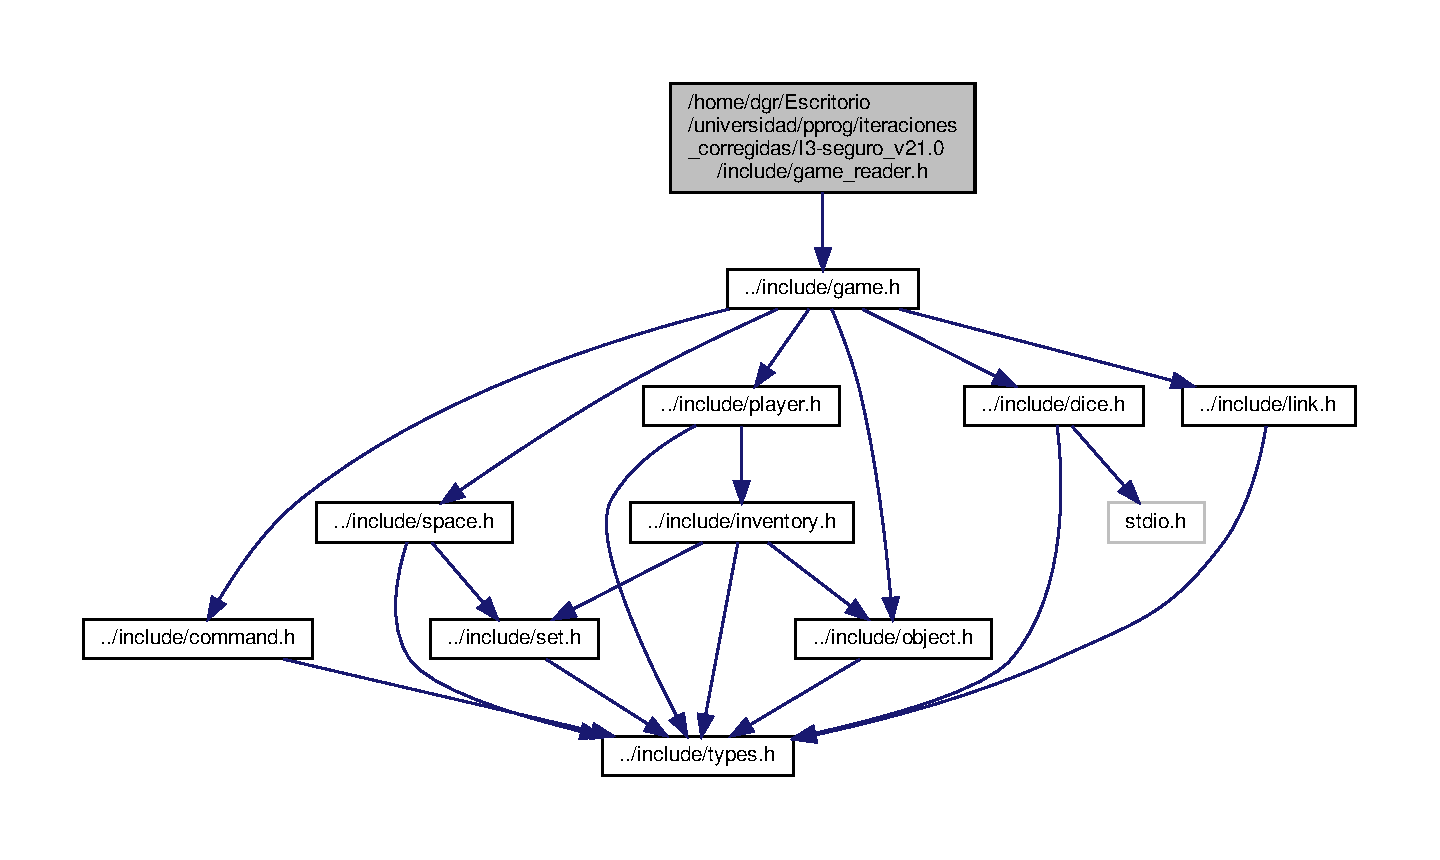
\includegraphics[width=350pt]{game__reader_8h__incl}
\end{center}
\end{figure}
This graph shows which files directly or indirectly include this file\+:
\nopagebreak
\begin{figure}[H]
\begin{center}
\leavevmode
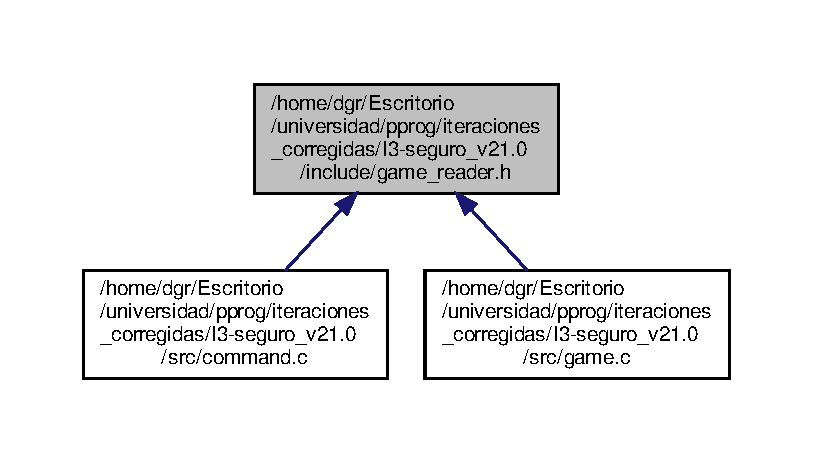
\includegraphics[width=350pt]{game__reader_8h__dep__incl}
\end{center}
\end{figure}
\subsection*{Functions}
\begin{DoxyCompactItemize}
\item 
\hyperlink{types_8h_a32c27cc471df37f4fc818d65de0a56c4}{S\+T\+A\+T\+US} \hyperlink{game__reader_8h_a1e0e4f4ede7bb399d6f33f66b7c38392}{game\+\_\+reader\+\_\+load\+\_\+spaces} (\hyperlink{game_8h_a57156d39c530aec3fba3a9dad8c2dc6a}{Game} $\ast$game, char $\ast$filename)
\begin{DoxyCompactList}\small\item\em load the spaces of the game, opening the file data.\+dat \end{DoxyCompactList}\item 
\hyperlink{types_8h_a32c27cc471df37f4fc818d65de0a56c4}{S\+T\+A\+T\+US} \hyperlink{game__reader_8h_a07d0cc9ec5cae35a9ad5dd7882357234}{game\+\_\+reader\+\_\+load\+\_\+objects} (\hyperlink{game_8h_a57156d39c530aec3fba3a9dad8c2dc6a}{Game} $\ast$game, char $\ast$filename)
\begin{DoxyCompactList}\small\item\em load the objects of the game, opening the file data.\+dat \end{DoxyCompactList}\item 
\hyperlink{types_8h_a32c27cc471df37f4fc818d65de0a56c4}{S\+T\+A\+T\+US} \hyperlink{game__reader_8h_a38c90d2eaaa4f9daed93df003d0f92f9}{game\+\_\+reader\+\_\+load\+\_\+player} (\hyperlink{game_8h_a57156d39c530aec3fba3a9dad8c2dc6a}{Game} $\ast$game, char $\ast$filename)
\begin{DoxyCompactList}\small\item\em load the player of the game, opening the file data.\+dat \end{DoxyCompactList}\item 
\hyperlink{types_8h_a32c27cc471df37f4fc818d65de0a56c4}{S\+T\+A\+T\+US} \hyperlink{game__reader_8h_aa47ab8dc1e29821281766ab359e8ac8b}{game\+\_\+reader\+\_\+load\+\_\+links} (\hyperlink{game_8h_a57156d39c530aec3fba3a9dad8c2dc6a}{Game} $\ast$game, char $\ast$filename)
\begin{DoxyCompactList}\small\item\em load the links of the game, opening the file data.\+dat \end{DoxyCompactList}\end{DoxyCompactItemize}


\subsection{Detailed Description}
Library to manage the load os spaces. 

\begin{DoxyVersion}{Version}
1.\+0 
\end{DoxyVersion}
\begin{DoxyDate}{Date}
08-\/02-\/2020 
\end{DoxyDate}
\begin{DoxyAuthor}{Author}
David Teófilo Garitagoitia Romero y José Manuel García Giráldez 
\end{DoxyAuthor}


\subsection{Function Documentation}
\mbox{\Hypertarget{game__reader_8h_aa47ab8dc1e29821281766ab359e8ac8b}\label{game__reader_8h_aa47ab8dc1e29821281766ab359e8ac8b}} 
\index{game\+\_\+reader.\+h@{game\+\_\+reader.\+h}!game\+\_\+reader\+\_\+load\+\_\+links@{game\+\_\+reader\+\_\+load\+\_\+links}}
\index{game\+\_\+reader\+\_\+load\+\_\+links@{game\+\_\+reader\+\_\+load\+\_\+links}!game\+\_\+reader.\+h@{game\+\_\+reader.\+h}}
\subsubsection{\texorpdfstring{game\+\_\+reader\+\_\+load\+\_\+links()}{game\_reader\_load\_links()}}
{\footnotesize\ttfamily \hyperlink{types_8h_a32c27cc471df37f4fc818d65de0a56c4}{S\+T\+A\+T\+US} game\+\_\+reader\+\_\+load\+\_\+links (\begin{DoxyParamCaption}\item[{\hyperlink{game_8h_a57156d39c530aec3fba3a9dad8c2dc6a}{Game} $\ast$}]{game,  }\item[{char $\ast$}]{filename }\end{DoxyParamCaption})}



load the links of the game, opening the file data.\+dat 

game\+\_\+reader\+\_\+load\+\_\+links

\begin{DoxyDate}{Date}
15-\/03-\/2019 
\end{DoxyDate}
\begin{DoxyAuthor}{Author}
\+: David Teófilo Garitagoitia Romero
\end{DoxyAuthor}

\begin{DoxyParams}{Parameters}
{\em game} & the game from which we will get the information \\
\hline
{\em filename} & the name of the file we work with \\
\hline
\end{DoxyParams}
\begin{DoxyReturn}{Returns}
the status of the file 
\end{DoxyReturn}
\mbox{\Hypertarget{game__reader_8h_a07d0cc9ec5cae35a9ad5dd7882357234}\label{game__reader_8h_a07d0cc9ec5cae35a9ad5dd7882357234}} 
\index{game\+\_\+reader.\+h@{game\+\_\+reader.\+h}!game\+\_\+reader\+\_\+load\+\_\+objects@{game\+\_\+reader\+\_\+load\+\_\+objects}}
\index{game\+\_\+reader\+\_\+load\+\_\+objects@{game\+\_\+reader\+\_\+load\+\_\+objects}!game\+\_\+reader.\+h@{game\+\_\+reader.\+h}}
\subsubsection{\texorpdfstring{game\+\_\+reader\+\_\+load\+\_\+objects()}{game\_reader\_load\_objects()}}
{\footnotesize\ttfamily \hyperlink{types_8h_a32c27cc471df37f4fc818d65de0a56c4}{S\+T\+A\+T\+US} game\+\_\+reader\+\_\+load\+\_\+objects (\begin{DoxyParamCaption}\item[{\hyperlink{game_8h_a57156d39c530aec3fba3a9dad8c2dc6a}{Game} $\ast$}]{game,  }\item[{char $\ast$}]{filename }\end{DoxyParamCaption})}



load the objects of the game, opening the file data.\+dat 

game\+\_\+reader\+\_\+load\+\_\+objects

\begin{DoxyDate}{Date}
06-\/03-\/2019 
\end{DoxyDate}
\begin{DoxyAuthor}{Author}
\+: David Teófilo Garitagoitia Romero
\end{DoxyAuthor}

\begin{DoxyParams}{Parameters}
{\em game} & the game from which we will get the information \\
\hline
{\em filename} & the name of the file we work with \\
\hline
\end{DoxyParams}
\begin{DoxyReturn}{Returns}
the status of the file 
\end{DoxyReturn}
\mbox{\Hypertarget{game__reader_8h_a38c90d2eaaa4f9daed93df003d0f92f9}\label{game__reader_8h_a38c90d2eaaa4f9daed93df003d0f92f9}} 
\index{game\+\_\+reader.\+h@{game\+\_\+reader.\+h}!game\+\_\+reader\+\_\+load\+\_\+player@{game\+\_\+reader\+\_\+load\+\_\+player}}
\index{game\+\_\+reader\+\_\+load\+\_\+player@{game\+\_\+reader\+\_\+load\+\_\+player}!game\+\_\+reader.\+h@{game\+\_\+reader.\+h}}
\subsubsection{\texorpdfstring{game\+\_\+reader\+\_\+load\+\_\+player()}{game\_reader\_load\_player()}}
{\footnotesize\ttfamily \hyperlink{types_8h_a32c27cc471df37f4fc818d65de0a56c4}{S\+T\+A\+T\+US} game\+\_\+reader\+\_\+load\+\_\+player (\begin{DoxyParamCaption}\item[{\hyperlink{game_8h_a57156d39c530aec3fba3a9dad8c2dc6a}{Game} $\ast$}]{game,  }\item[{char $\ast$}]{filename }\end{DoxyParamCaption})}



load the player of the game, opening the file data.\+dat 

game\+\_\+reader\+\_\+load\+\_\+player

\begin{DoxyDate}{Date}
15-\/03-\/2019 
\end{DoxyDate}
\begin{DoxyAuthor}{Author}
\+: David Teófilo Garitagoitia Romero
\end{DoxyAuthor}

\begin{DoxyParams}{Parameters}
{\em game} & the game from which we will get the information \\
\hline
{\em filename} & the name of the file we work with \\
\hline
\end{DoxyParams}
\begin{DoxyReturn}{Returns}
the status of the file 
\end{DoxyReturn}
\mbox{\Hypertarget{game__reader_8h_a1e0e4f4ede7bb399d6f33f66b7c38392}\label{game__reader_8h_a1e0e4f4ede7bb399d6f33f66b7c38392}} 
\index{game\+\_\+reader.\+h@{game\+\_\+reader.\+h}!game\+\_\+reader\+\_\+load\+\_\+spaces@{game\+\_\+reader\+\_\+load\+\_\+spaces}}
\index{game\+\_\+reader\+\_\+load\+\_\+spaces@{game\+\_\+reader\+\_\+load\+\_\+spaces}!game\+\_\+reader.\+h@{game\+\_\+reader.\+h}}
\subsubsection{\texorpdfstring{game\+\_\+reader\+\_\+load\+\_\+spaces()}{game\_reader\_load\_spaces()}}
{\footnotesize\ttfamily \hyperlink{types_8h_a32c27cc471df37f4fc818d65de0a56c4}{S\+T\+A\+T\+US} game\+\_\+reader\+\_\+load\+\_\+spaces (\begin{DoxyParamCaption}\item[{\hyperlink{game_8h_a57156d39c530aec3fba3a9dad8c2dc6a}{Game} $\ast$}]{game,  }\item[{char $\ast$}]{filename }\end{DoxyParamCaption})}



load the spaces of the game, opening the file data.\+dat 

game\+\_\+reader\+\_\+load\+\_\+spaces

\begin{DoxyDate}{Date}
06-\/02-\/2019 
\end{DoxyDate}
\begin{DoxyAuthor}{Author}
José Manuel García Giráldez
\end{DoxyAuthor}

\begin{DoxyParams}{Parameters}
{\em game} & the game from which we will get the information \\
\hline
{\em filename} & the name of the file we work with \\
\hline
\end{DoxyParams}
\begin{DoxyReturn}{Returns}
the status of the file 
\end{DoxyReturn}

\hypertarget{graphic__engine_8h}{}\section{include/graphic\+\_\+engine.h File Reference}
\label{graphic__engine_8h}\index{include/graphic\+\_\+engine.\+h@{include/graphic\+\_\+engine.\+h}}


It defines a textual graphic engine.  


{\ttfamily \#include \char`\"{}../include/game.\+h\char`\"{}}\newline
Include dependency graph for graphic\+\_\+engine.\+h\+:\nopagebreak
\begin{figure}[H]
\begin{center}
\leavevmode
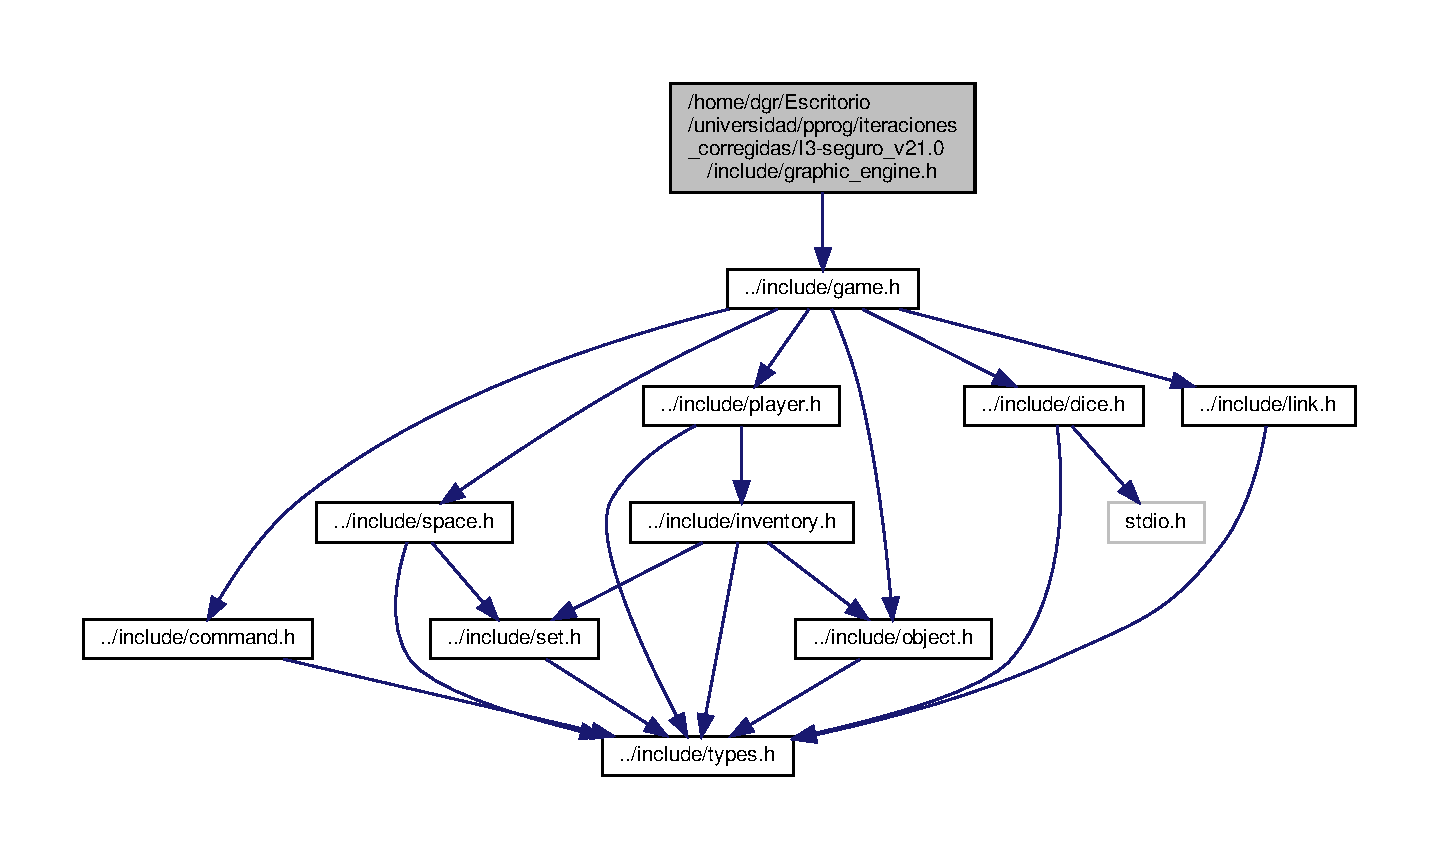
\includegraphics[width=350pt]{graphic__engine_8h__incl}
\end{center}
\end{figure}
This graph shows which files directly or indirectly include this file\+:\nopagebreak
\begin{figure}[H]
\begin{center}
\leavevmode
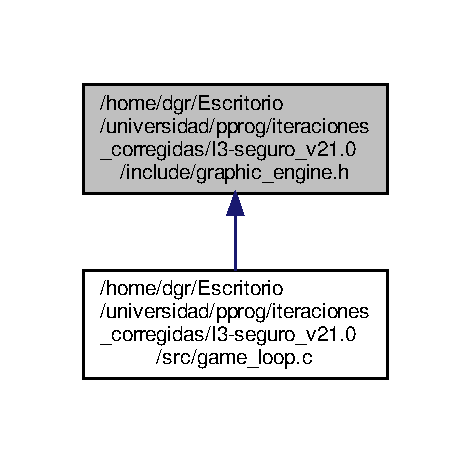
\includegraphics[width=204pt]{graphic__engine_8h__dep__incl}
\end{center}
\end{figure}
\subsection*{Typedefs}
\begin{DoxyCompactItemize}
\item 
typedef struct \hyperlink{struct__Graphic__engine}{\+\_\+\+Graphic\+\_\+engine} \hyperlink{graphic__engine_8h_ae1bc5cdbfce93098f066274fdea49af1}{Graphic\+\_\+engine}
\begin{DoxyCompactList}\small\item\em A type definition for a graphic engine. \end{DoxyCompactList}\end{DoxyCompactItemize}
\subsection*{Functions}
\begin{DoxyCompactItemize}
\item 
\hyperlink{graphic__engine_8h_ae1bc5cdbfce93098f066274fdea49af1}{Graphic\+\_\+engine} $\ast$ \hyperlink{graphic__engine_8h_a8c3d9abe7282bee1d77d23ea80a4bdec}{graphic\+\_\+engine\+\_\+create} ()
\begin{DoxyCompactList}\small\item\em create graphic engine \end{DoxyCompactList}\item 
void \hyperlink{graphic__engine_8h_a5a5eac4ef2033c5ad71aa6895f362f79}{graphic\+\_\+engine\+\_\+destroy} (\hyperlink{graphic__engine_8h_ae1bc5cdbfce93098f066274fdea49af1}{Graphic\+\_\+engine} $\ast$ge)
\begin{DoxyCompactList}\small\item\em destroy graphic engine \end{DoxyCompactList}\item 
void \hyperlink{graphic__engine_8h_a06241143501ef0b88082933fb5fd5b0b}{graphic\+\_\+engine\+\_\+paint\+\_\+game} (\hyperlink{graphic__engine_8h_ae1bc5cdbfce93098f066274fdea49af1}{Graphic\+\_\+engine} $\ast$ge, \hyperlink{game_8h_a57156d39c530aec3fba3a9dad8c2dc6a}{Game} $\ast$game, F\+I\+LE $\ast$file)
\begin{DoxyCompactList}\small\item\em paint the game \end{DoxyCompactList}\item 
void \hyperlink{graphic__engine_8h_a112605879db4582a6d9cd6c12bd0e90c}{graphic\+\_\+engine\+\_\+write\+\_\+command} (\hyperlink{graphic__engine_8h_ae1bc5cdbfce93098f066274fdea49af1}{Graphic\+\_\+engine} $\ast$ge, char $\ast$str)
\begin{DoxyCompactList}\small\item\em write the command \end{DoxyCompactList}\item 
void \hyperlink{graphic__engine_8h_a1434353adc00dbe4e351a3af57fb3fe8}{graphic\+\_\+engine\+\_\+paint\+\_\+intro} (\hyperlink{graphic__engine_8h_ae1bc5cdbfce93098f066274fdea49af1}{Graphic\+\_\+engine} $\ast$ge, \hyperlink{game_8h_a57156d39c530aec3fba3a9dad8c2dc6a}{Game} $\ast$game, char $\ast$f)
\begin{DoxyCompactList}\small\item\em paint the intro \end{DoxyCompactList}\item 
void \hyperlink{graphic__engine_8h_a7082fc33231792ba9590fb2e558b5c45}{graphic\+\_\+engine\+\_\+paint\+\_\+end} (\hyperlink{graphic__engine_8h_ae1bc5cdbfce93098f066274fdea49af1}{Graphic\+\_\+engine} $\ast$ge, \hyperlink{game_8h_a57156d39c530aec3fba3a9dad8c2dc6a}{Game} $\ast$game, char $\ast$f)
\begin{DoxyCompactList}\small\item\em paint the end \end{DoxyCompactList}\end{DoxyCompactItemize}


\subsection{Detailed Description}
It defines a textual graphic engine. 

\begin{DoxyAuthor}{Author}
Instructors of P\+P\+R\+OG, David Teófilo Garitagoitia Romero 
\end{DoxyAuthor}
\begin{DoxyVersion}{Version}
1.\+0 
\end{DoxyVersion}
\begin{DoxyDate}{Date}
18-\/01-\/2017 
\end{DoxyDate}
\begin{DoxyCopyright}{Copyright}
G\+NU Public License 
\end{DoxyCopyright}


\subsection{Typedef Documentation}
\mbox{\Hypertarget{graphic__engine_8h_ae1bc5cdbfce93098f066274fdea49af1}\label{graphic__engine_8h_ae1bc5cdbfce93098f066274fdea49af1}} 
\index{graphic\+\_\+engine.\+h@{graphic\+\_\+engine.\+h}!Graphic\+\_\+engine@{Graphic\+\_\+engine}}
\index{Graphic\+\_\+engine@{Graphic\+\_\+engine}!graphic\+\_\+engine.\+h@{graphic\+\_\+engine.\+h}}
\subsubsection{\texorpdfstring{Graphic\+\_\+engine}{Graphic\_engine}}
{\footnotesize\ttfamily typedef struct \hyperlink{struct__Graphic__engine}{\+\_\+\+Graphic\+\_\+engine} \hyperlink{graphic__engine_8h_ae1bc5cdbfce93098f066274fdea49af1}{Graphic\+\_\+engine}}



A type definition for a graphic engine. 

Details. 

\subsection{Function Documentation}
\mbox{\Hypertarget{graphic__engine_8h_a8c3d9abe7282bee1d77d23ea80a4bdec}\label{graphic__engine_8h_a8c3d9abe7282bee1d77d23ea80a4bdec}} 
\index{graphic\+\_\+engine.\+h@{graphic\+\_\+engine.\+h}!graphic\+\_\+engine\+\_\+create@{graphic\+\_\+engine\+\_\+create}}
\index{graphic\+\_\+engine\+\_\+create@{graphic\+\_\+engine\+\_\+create}!graphic\+\_\+engine.\+h@{graphic\+\_\+engine.\+h}}
\subsubsection{\texorpdfstring{graphic\+\_\+engine\+\_\+create()}{graphic\_engine\_create()}}
{\footnotesize\ttfamily \hyperlink{graphic__engine_8h_ae1bc5cdbfce93098f066274fdea49af1}{Graphic\+\_\+engine}$\ast$ graphic\+\_\+engine\+\_\+create (\begin{DoxyParamCaption}{ }\end{DoxyParamCaption})}



create graphic engine 

graphic\+\_\+engine\+\_\+create

\begin{DoxyDate}{Date}
13-\/01-\/2015 
\end{DoxyDate}
\begin{DoxyAuthor}{Author}
\+: Instructors of P\+P\+R\+OG 
\end{DoxyAuthor}
\begin{DoxyReturn}{Returns}
the address of the graphic engine created 
\end{DoxyReturn}
\mbox{\Hypertarget{graphic__engine_8h_a5a5eac4ef2033c5ad71aa6895f362f79}\label{graphic__engine_8h_a5a5eac4ef2033c5ad71aa6895f362f79}} 
\index{graphic\+\_\+engine.\+h@{graphic\+\_\+engine.\+h}!graphic\+\_\+engine\+\_\+destroy@{graphic\+\_\+engine\+\_\+destroy}}
\index{graphic\+\_\+engine\+\_\+destroy@{graphic\+\_\+engine\+\_\+destroy}!graphic\+\_\+engine.\+h@{graphic\+\_\+engine.\+h}}
\subsubsection{\texorpdfstring{graphic\+\_\+engine\+\_\+destroy()}{graphic\_engine\_destroy()}}
{\footnotesize\ttfamily void graphic\+\_\+engine\+\_\+destroy (\begin{DoxyParamCaption}\item[{\hyperlink{graphic__engine_8h_ae1bc5cdbfce93098f066274fdea49af1}{Graphic\+\_\+engine} $\ast$}]{ge }\end{DoxyParamCaption})}



destroy graphic engine 

graphic\+\_\+engine\+\_\+destroy

\begin{DoxyDate}{Date}
13-\/01-\/2015 
\end{DoxyDate}
\begin{DoxyAuthor}{Author}
\+: Instructors of P\+P\+R\+OG 
\end{DoxyAuthor}
\begin{DoxyReturn}{Returns}

\end{DoxyReturn}
\mbox{\Hypertarget{graphic__engine_8h_a7082fc33231792ba9590fb2e558b5c45}\label{graphic__engine_8h_a7082fc33231792ba9590fb2e558b5c45}} 
\index{graphic\+\_\+engine.\+h@{graphic\+\_\+engine.\+h}!graphic\+\_\+engine\+\_\+paint\+\_\+end@{graphic\+\_\+engine\+\_\+paint\+\_\+end}}
\index{graphic\+\_\+engine\+\_\+paint\+\_\+end@{graphic\+\_\+engine\+\_\+paint\+\_\+end}!graphic\+\_\+engine.\+h@{graphic\+\_\+engine.\+h}}
\subsubsection{\texorpdfstring{graphic\+\_\+engine\+\_\+paint\+\_\+end()}{graphic\_engine\_paint\_end()}}
{\footnotesize\ttfamily void graphic\+\_\+engine\+\_\+paint\+\_\+end (\begin{DoxyParamCaption}\item[{\hyperlink{graphic__engine_8h_ae1bc5cdbfce93098f066274fdea49af1}{Graphic\+\_\+engine} $\ast$}]{ge,  }\item[{\hyperlink{game_8h_a57156d39c530aec3fba3a9dad8c2dc6a}{Game} $\ast$}]{game,  }\item[{char $\ast$}]{f }\end{DoxyParamCaption})}



paint the end 

graphic\+\_\+engine\+\_\+paint\+\_\+intro

\begin{DoxyDate}{Date}
5-\/05-\/2020 
\end{DoxyDate}

\begin{DoxyParams}{Parameters}
{\em ge} & pointer to graphic\+\_\+engine \\
\hline
{\em game} & pointer to game structure \\
\hline
{\em f} & file with the intro \\
\hline
\end{DoxyParams}
\begin{DoxyAuthor}{Author}
\+: David Teófilo Garitagoitia Romero 
\end{DoxyAuthor}
\begin{DoxyReturn}{Returns}

\end{DoxyReturn}
\mbox{\Hypertarget{graphic__engine_8h_a06241143501ef0b88082933fb5fd5b0b}\label{graphic__engine_8h_a06241143501ef0b88082933fb5fd5b0b}} 
\index{graphic\+\_\+engine.\+h@{graphic\+\_\+engine.\+h}!graphic\+\_\+engine\+\_\+paint\+\_\+game@{graphic\+\_\+engine\+\_\+paint\+\_\+game}}
\index{graphic\+\_\+engine\+\_\+paint\+\_\+game@{graphic\+\_\+engine\+\_\+paint\+\_\+game}!graphic\+\_\+engine.\+h@{graphic\+\_\+engine.\+h}}
\subsubsection{\texorpdfstring{graphic\+\_\+engine\+\_\+paint\+\_\+game()}{graphic\_engine\_paint\_game()}}
{\footnotesize\ttfamily void graphic\+\_\+engine\+\_\+paint\+\_\+game (\begin{DoxyParamCaption}\item[{\hyperlink{graphic__engine_8h_ae1bc5cdbfce93098f066274fdea49af1}{Graphic\+\_\+engine} $\ast$}]{ge,  }\item[{\hyperlink{game_8h_a57156d39c530aec3fba3a9dad8c2dc6a}{Game} $\ast$}]{game,  }\item[{F\+I\+LE $\ast$}]{file }\end{DoxyParamCaption})}



paint the game 

graphic\+\_\+engine\+\_\+paint\+\_\+game

\begin{DoxyDate}{Date}
13-\/01-\/2015 
\end{DoxyDate}

\begin{DoxyParams}{Parameters}
{\em ge} & pointer to graphic\+\_\+engine \\
\hline
{\em game} & pointer to game structure \\
\hline
{\em file} & pointer to the file \\
\hline
\end{DoxyParams}
\begin{DoxyAuthor}{Author}
\+: Instructors of P\+P\+R\+OG 
\end{DoxyAuthor}
\begin{DoxyReturn}{Returns}

\end{DoxyReturn}
\mbox{\Hypertarget{graphic__engine_8h_a1434353adc00dbe4e351a3af57fb3fe8}\label{graphic__engine_8h_a1434353adc00dbe4e351a3af57fb3fe8}} 
\index{graphic\+\_\+engine.\+h@{graphic\+\_\+engine.\+h}!graphic\+\_\+engine\+\_\+paint\+\_\+intro@{graphic\+\_\+engine\+\_\+paint\+\_\+intro}}
\index{graphic\+\_\+engine\+\_\+paint\+\_\+intro@{graphic\+\_\+engine\+\_\+paint\+\_\+intro}!graphic\+\_\+engine.\+h@{graphic\+\_\+engine.\+h}}
\subsubsection{\texorpdfstring{graphic\+\_\+engine\+\_\+paint\+\_\+intro()}{graphic\_engine\_paint\_intro()}}
{\footnotesize\ttfamily void graphic\+\_\+engine\+\_\+paint\+\_\+intro (\begin{DoxyParamCaption}\item[{\hyperlink{graphic__engine_8h_ae1bc5cdbfce93098f066274fdea49af1}{Graphic\+\_\+engine} $\ast$}]{ge,  }\item[{\hyperlink{game_8h_a57156d39c530aec3fba3a9dad8c2dc6a}{Game} $\ast$}]{game,  }\item[{char $\ast$}]{f }\end{DoxyParamCaption})}



paint the intro 

graphic\+\_\+engine\+\_\+paint\+\_\+intro

\begin{DoxyDate}{Date}
5-\/05-\/2020 
\end{DoxyDate}

\begin{DoxyParams}{Parameters}
{\em ge} & pointer to graphic\+\_\+engine \\
\hline
{\em game} & pointer to game structure \\
\hline
{\em f} & file with the intro \\
\hline
\end{DoxyParams}
\begin{DoxyAuthor}{Author}
\+: David Teófilo Garitagoitia Romero 
\end{DoxyAuthor}
\begin{DoxyReturn}{Returns}

\end{DoxyReturn}
\mbox{\Hypertarget{graphic__engine_8h_a112605879db4582a6d9cd6c12bd0e90c}\label{graphic__engine_8h_a112605879db4582a6d9cd6c12bd0e90c}} 
\index{graphic\+\_\+engine.\+h@{graphic\+\_\+engine.\+h}!graphic\+\_\+engine\+\_\+write\+\_\+command@{graphic\+\_\+engine\+\_\+write\+\_\+command}}
\index{graphic\+\_\+engine\+\_\+write\+\_\+command@{graphic\+\_\+engine\+\_\+write\+\_\+command}!graphic\+\_\+engine.\+h@{graphic\+\_\+engine.\+h}}
\subsubsection{\texorpdfstring{graphic\+\_\+engine\+\_\+write\+\_\+command()}{graphic\_engine\_write\_command()}}
{\footnotesize\ttfamily void graphic\+\_\+engine\+\_\+write\+\_\+command (\begin{DoxyParamCaption}\item[{\hyperlink{graphic__engine_8h_ae1bc5cdbfce93098f066274fdea49af1}{Graphic\+\_\+engine} $\ast$}]{ge,  }\item[{char $\ast$}]{str }\end{DoxyParamCaption})}



write the command 

graphic\+\_\+engine\+\_\+write\+\_\+command

\begin{DoxyDate}{Date}
13-\/01-\/2015 
\end{DoxyDate}
\begin{DoxyAuthor}{Author}
\+: Instructors of P\+P\+R\+OG 
\end{DoxyAuthor}
\begin{DoxyReturn}{Returns}

\end{DoxyReturn}

\hypertarget{inventory_8h}{}\section{/home/dgr/\+Escritorio/universidad/pprog/iteraciones\+\_\+corregidas/\+I3-\/seguro\+\_\+v21.0/include/inventory.h File Reference}
\label{inventory_8h}\index{/home/dgr/\+Escritorio/universidad/pprog/iteraciones\+\_\+corregidas/\+I3-\/seguro\+\_\+v21.\+0/include/inventory.\+h@{/home/dgr/\+Escritorio/universidad/pprog/iteraciones\+\_\+corregidas/\+I3-\/seguro\+\_\+v21.\+0/include/inventory.\+h}}


It defines the inventory interface for each command.  


{\ttfamily \#include \char`\"{}../include/types.\+h\char`\"{}}\newline
{\ttfamily \#include \char`\"{}../include/set.\+h\char`\"{}}\newline
{\ttfamily \#include \char`\"{}../include/object.\+h\char`\"{}}\newline
Include dependency graph for inventory.\+h\+:
\nopagebreak
\begin{figure}[H]
\begin{center}
\leavevmode
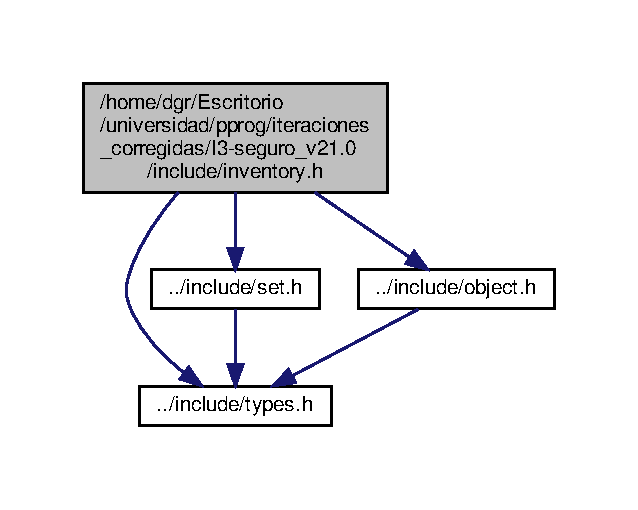
\includegraphics[width=306pt]{inventory_8h__incl}
\end{center}
\end{figure}
This graph shows which files directly or indirectly include this file\+:
\nopagebreak
\begin{figure}[H]
\begin{center}
\leavevmode
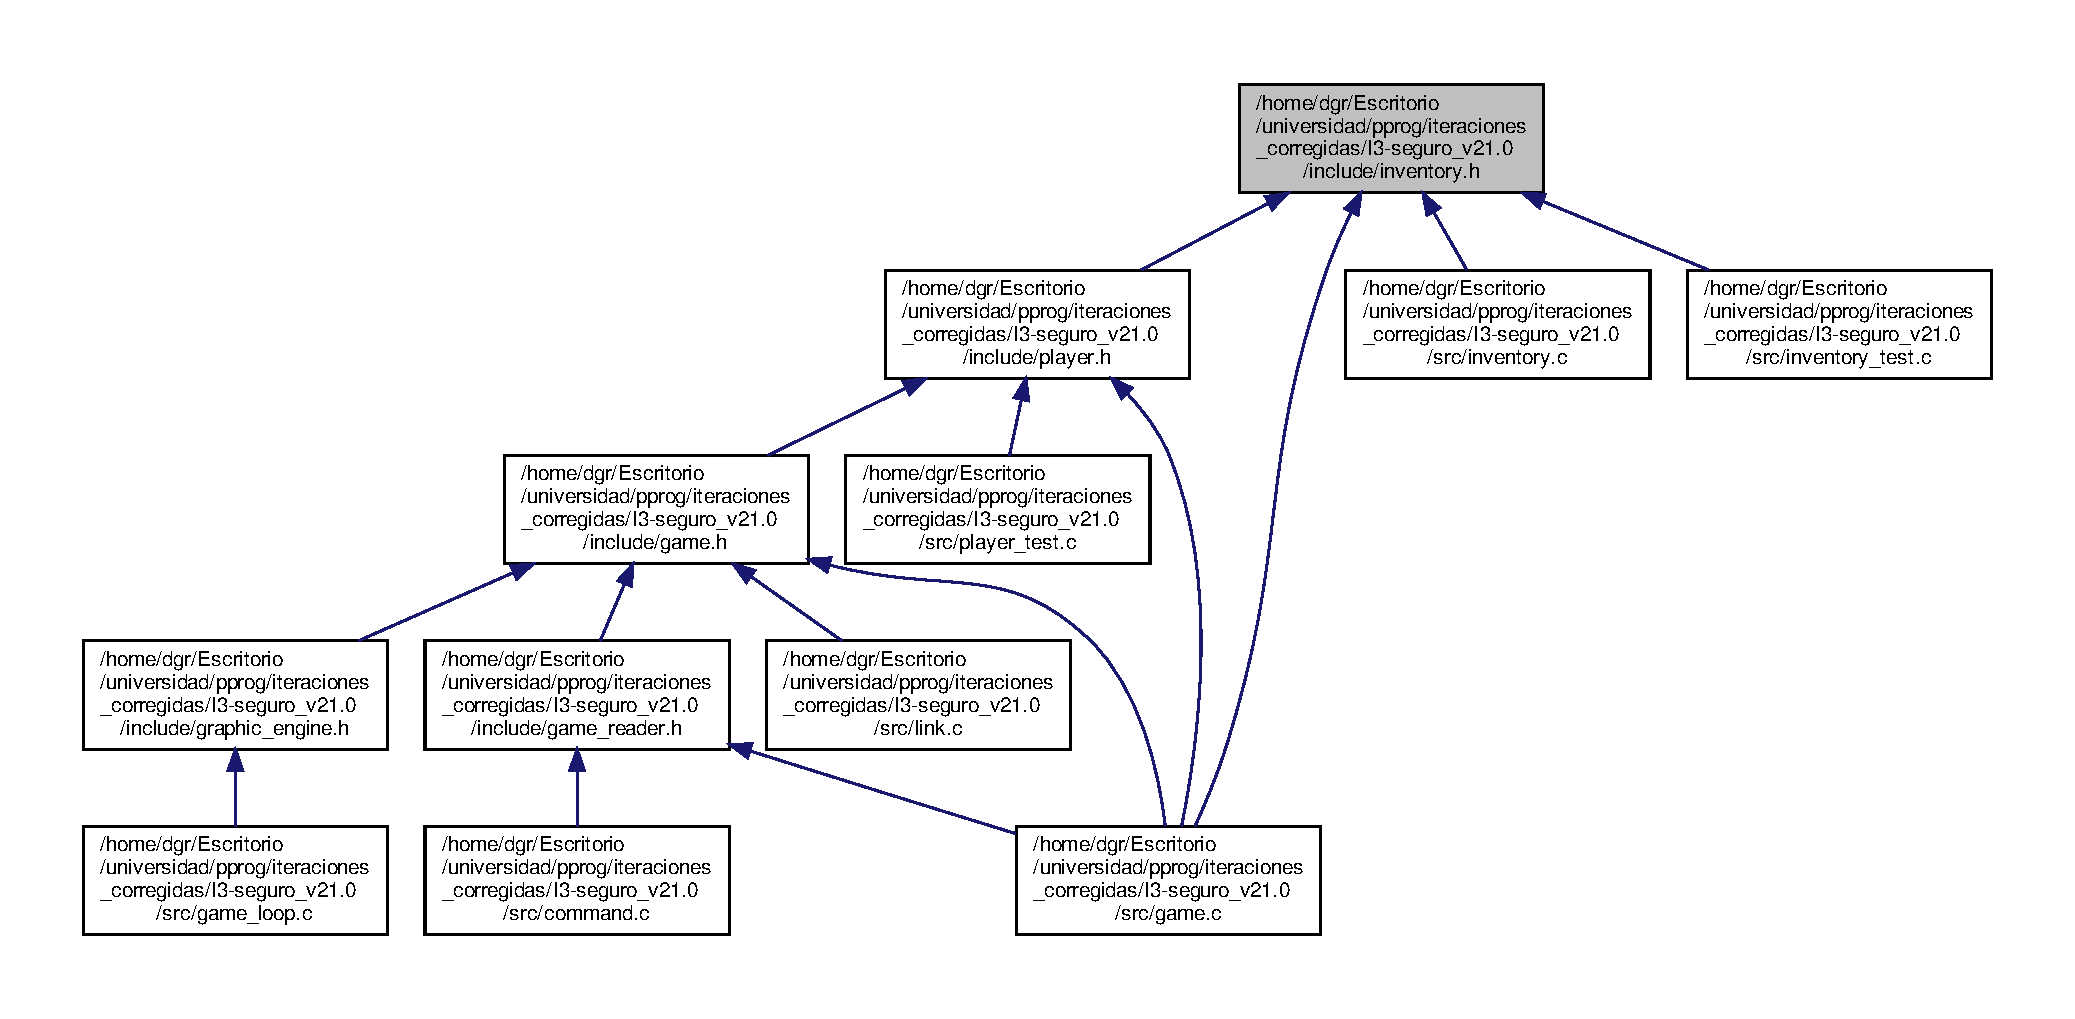
\includegraphics[width=350pt]{inventory_8h__dep__incl}
\end{center}
\end{figure}
\subsection*{Typedefs}
\begin{DoxyCompactItemize}
\item 
typedef struct \hyperlink{struct__Inventory}{\+\_\+\+Inventory} \hyperlink{inventory_8h_a2253bf64ac4ce6a9c1d6f39c0b0d32a3}{Inventory}
\begin{DoxyCompactList}\small\item\em A type definition for a inventory. \end{DoxyCompactList}\end{DoxyCompactItemize}
\subsection*{Functions}
\begin{DoxyCompactItemize}
\item 
\hyperlink{inventory_8h_a2253bf64ac4ce6a9c1d6f39c0b0d32a3}{Inventory} $\ast$ \hyperlink{inventory_8h_a84f90137d8559068d8292b8d10c675a1}{inventory\+\_\+create} (\hyperlink{types_8h_a845e604fb28f7e3d97549da3448149d3}{Id} id, int max)
\begin{DoxyCompactList}\small\item\em Create the inventory. \end{DoxyCompactList}\item 
\hyperlink{types_8h_a845e604fb28f7e3d97549da3448149d3}{Id} \hyperlink{inventory_8h_a77f843a5f77feedf0812662e6b3dbeca}{inventory\+\_\+get\+\_\+id} (\hyperlink{inventory_8h_a2253bf64ac4ce6a9c1d6f39c0b0d32a3}{Inventory} $\ast$inventory)
\begin{DoxyCompactList}\small\item\em Return the id of the inventory. \end{DoxyCompactList}\item 
\hyperlink{types_8h_a32c27cc471df37f4fc818d65de0a56c4}{S\+T\+A\+T\+US} \hyperlink{inventory_8h_a690c5b171251c27a628f0ecaaaf6b9ce}{inventory\+\_\+destroy} (\hyperlink{inventory_8h_a2253bf64ac4ce6a9c1d6f39c0b0d32a3}{Inventory} $\ast$inventory)
\begin{DoxyCompactList}\small\item\em Destroy the inventory. \end{DoxyCompactList}\item 
\hyperlink{types_8h_a32c27cc471df37f4fc818d65de0a56c4}{S\+T\+A\+T\+US} \hyperlink{inventory_8h_a4f3b96537e64ffc63731555e116c3adb}{inventory\+\_\+add} (\hyperlink{inventory_8h_a2253bf64ac4ce6a9c1d6f39c0b0d32a3}{Inventory} $\ast$inventory, \hyperlink{types_8h_a845e604fb28f7e3d97549da3448149d3}{Id} id)
\begin{DoxyCompactList}\small\item\em Add the object to the inventory. \end{DoxyCompactList}\item 
\hyperlink{types_8h_a32c27cc471df37f4fc818d65de0a56c4}{S\+T\+A\+T\+US} \hyperlink{inventory_8h_a348efe95855b9ecad72ea3b6bf1ce8c4}{inventory\+\_\+dell} (\hyperlink{inventory_8h_a2253bf64ac4ce6a9c1d6f39c0b0d32a3}{Inventory} $\ast$inventory, \hyperlink{types_8h_a845e604fb28f7e3d97549da3448149d3}{Id} id)
\begin{DoxyCompactList}\small\item\em Delete the object of the inventory. \end{DoxyCompactList}\item 
\hyperlink{set_8h_a6d3b7f7c92cbb4577ef3ef7ddbf93161}{Set} $\ast$ \hyperlink{inventory_8h_a6a1f9cdbffc20d4283f09635c98ffb83}{inventory\+\_\+get\+\_\+inside} (\hyperlink{inventory_8h_a2253bf64ac4ce6a9c1d6f39c0b0d32a3}{Inventory} $\ast$inventory)
\begin{DoxyCompactList}\small\item\em Return the set of the inventory. \end{DoxyCompactList}\item 
\hyperlink{types_8h_a3e5b8192e7d9ffaf3542f1210aec18dd}{B\+O\+OL} \hyperlink{inventory_8h_a7da45e3f52165fd1e3a51c95aa6f78f8}{inventory\+\_\+is\+\_\+object} (\hyperlink{inventory_8h_a2253bf64ac4ce6a9c1d6f39c0b0d32a3}{Inventory} $\ast$inventory, \hyperlink{types_8h_a845e604fb28f7e3d97549da3448149d3}{Id} id)
\begin{DoxyCompactList}\small\item\em check if the object is in inventory \end{DoxyCompactList}\item 
int \hyperlink{inventory_8h_aac41dfbea9df9fcfbbebfec318ddd636}{inventory\+\_\+get\+\_\+max} (\hyperlink{inventory_8h_a2253bf64ac4ce6a9c1d6f39c0b0d32a3}{Inventory} $\ast$inventory)
\begin{DoxyCompactList}\small\item\em return the max number of objects of an inventory \end{DoxyCompactList}\item 
\hyperlink{types_8h_a3e5b8192e7d9ffaf3542f1210aec18dd}{B\+O\+OL} \hyperlink{inventory_8h_a31ce870d22db2381928f052c77b28288}{inventory\+\_\+is\+\_\+full} (\hyperlink{inventory_8h_a2253bf64ac4ce6a9c1d6f39c0b0d32a3}{Inventory} $\ast$inventory)
\begin{DoxyCompactList}\small\item\em check if the inventory is full \end{DoxyCompactList}\item 
\hyperlink{types_8h_a3e5b8192e7d9ffaf3542f1210aec18dd}{B\+O\+OL} \hyperlink{inventory_8h_a5be8b836d5bb5a948aab616ef404b1cd}{inventory\+\_\+is\+\_\+emty} (\hyperlink{inventory_8h_a2253bf64ac4ce6a9c1d6f39c0b0d32a3}{Inventory} $\ast$inventory)
\begin{DoxyCompactList}\small\item\em check if the inventory is empty \end{DoxyCompactList}\item 
void \hyperlink{inventory_8h_ad5b213ff8ab4ee5f6654cfe9d0107ea2}{inventory\+\_\+print} (F\+I\+LE $\ast$f, \hyperlink{inventory_8h_a2253bf64ac4ce6a9c1d6f39c0b0d32a3}{Inventory} $\ast$inventory)
\begin{DoxyCompactList}\small\item\em Print the inventory and on a file given. \end{DoxyCompactList}\end{DoxyCompactItemize}


\subsection{Detailed Description}
It defines the inventory interface for each command. 

\begin{DoxyAuthor}{Author}
Diego Grande Camarero, David Teófilo Garitagoitia Romero y Daniel Cerrato Sánchez 
\end{DoxyAuthor}
\begin{DoxyVersion}{Version}
1.\+0 
\end{DoxyVersion}
\begin{DoxyDate}{Date}
13-\/03-\/2020 
\end{DoxyDate}
\begin{DoxyCopyright}{Copyright}
G\+NU Public License 
\end{DoxyCopyright}


\subsection{Typedef Documentation}
\mbox{\Hypertarget{inventory_8h_a2253bf64ac4ce6a9c1d6f39c0b0d32a3}\label{inventory_8h_a2253bf64ac4ce6a9c1d6f39c0b0d32a3}} 
\index{inventory.\+h@{inventory.\+h}!Inventory@{Inventory}}
\index{Inventory@{Inventory}!inventory.\+h@{inventory.\+h}}
\subsubsection{\texorpdfstring{Inventory}{Inventory}}
{\footnotesize\ttfamily typedef struct \hyperlink{struct__Inventory}{\+\_\+\+Inventory} \hyperlink{inventory_8h_a2253bf64ac4ce6a9c1d6f39c0b0d32a3}{Inventory}}



A type definition for a inventory. 

Details. 

\subsection{Function Documentation}
\mbox{\Hypertarget{inventory_8h_a4f3b96537e64ffc63731555e116c3adb}\label{inventory_8h_a4f3b96537e64ffc63731555e116c3adb}} 
\index{inventory.\+h@{inventory.\+h}!inventory\+\_\+add@{inventory\+\_\+add}}
\index{inventory\+\_\+add@{inventory\+\_\+add}!inventory.\+h@{inventory.\+h}}
\subsubsection{\texorpdfstring{inventory\+\_\+add()}{inventory\_add()}}
{\footnotesize\ttfamily \hyperlink{types_8h_a32c27cc471df37f4fc818d65de0a56c4}{S\+T\+A\+T\+US} inventory\+\_\+add (\begin{DoxyParamCaption}\item[{\hyperlink{inventory_8h_a2253bf64ac4ce6a9c1d6f39c0b0d32a3}{Inventory} $\ast$}]{inventory,  }\item[{\hyperlink{types_8h_a845e604fb28f7e3d97549da3448149d3}{Id}}]{id }\end{DoxyParamCaption})}



Add the object to the inventory. 

\begin{DoxyDate}{Date}
14-\/03-\/2020 
\end{DoxyDate}
\begin{DoxyAuthor}{Author}
\+: Diego Grande Camarero
\end{DoxyAuthor}

\begin{DoxyParams}{Parameters}
{\em inventory} & Pointer to the inventory \\
\hline
{\em id} & The object id \\
\hline
\end{DoxyParams}
\begin{DoxyReturn}{Returns}
Ok if there was no problem, E\+R\+R\+OR if not 
\end{DoxyReturn}
\mbox{\Hypertarget{inventory_8h_a84f90137d8559068d8292b8d10c675a1}\label{inventory_8h_a84f90137d8559068d8292b8d10c675a1}} 
\index{inventory.\+h@{inventory.\+h}!inventory\+\_\+create@{inventory\+\_\+create}}
\index{inventory\+\_\+create@{inventory\+\_\+create}!inventory.\+h@{inventory.\+h}}
\subsubsection{\texorpdfstring{inventory\+\_\+create()}{inventory\_create()}}
{\footnotesize\ttfamily \hyperlink{inventory_8h_a2253bf64ac4ce6a9c1d6f39c0b0d32a3}{Inventory}$\ast$ inventory\+\_\+create (\begin{DoxyParamCaption}\item[{\hyperlink{types_8h_a845e604fb28f7e3d97549da3448149d3}{Id}}]{id,  }\item[{int}]{max }\end{DoxyParamCaption})}



Create the inventory. 

inventory\+\_\+create Create a new inventory

\begin{DoxyDate}{Date}
14-\/03-\/2020 
\end{DoxyDate}
\begin{DoxyAuthor}{Author}
\+: Diego Grande Camarero
\end{DoxyAuthor}

\begin{DoxyParams}{Parameters}
{\em id} & id of the inventory \\
\hline
{\em max} & max number of objects it will contain \\
\hline
\end{DoxyParams}
\begin{DoxyReturn}{Returns}
the new inventory that has been created 
\end{DoxyReturn}
\mbox{\Hypertarget{inventory_8h_a348efe95855b9ecad72ea3b6bf1ce8c4}\label{inventory_8h_a348efe95855b9ecad72ea3b6bf1ce8c4}} 
\index{inventory.\+h@{inventory.\+h}!inventory\+\_\+dell@{inventory\+\_\+dell}}
\index{inventory\+\_\+dell@{inventory\+\_\+dell}!inventory.\+h@{inventory.\+h}}
\subsubsection{\texorpdfstring{inventory\+\_\+dell()}{inventory\_dell()}}
{\footnotesize\ttfamily \hyperlink{types_8h_a32c27cc471df37f4fc818d65de0a56c4}{S\+T\+A\+T\+US} inventory\+\_\+dell (\begin{DoxyParamCaption}\item[{\hyperlink{inventory_8h_a2253bf64ac4ce6a9c1d6f39c0b0d32a3}{Inventory} $\ast$}]{inventory,  }\item[{\hyperlink{types_8h_a845e604fb28f7e3d97549da3448149d3}{Id}}]{id }\end{DoxyParamCaption})}



Delete the object of the inventory. 

\begin{DoxyDate}{Date}
14-\/03-\/2020 
\end{DoxyDate}
\begin{DoxyAuthor}{Author}
Diego Grande Camarero
\end{DoxyAuthor}

\begin{DoxyParams}{Parameters}
{\em inventory} & Pointer to the inventory \\
\hline
{\em id} & id of the object \\
\hline
\end{DoxyParams}
\begin{DoxyReturn}{Returns}
Ok if there was no problem, E\+R\+R\+OR if not 
\end{DoxyReturn}
\mbox{\Hypertarget{inventory_8h_a690c5b171251c27a628f0ecaaaf6b9ce}\label{inventory_8h_a690c5b171251c27a628f0ecaaaf6b9ce}} 
\index{inventory.\+h@{inventory.\+h}!inventory\+\_\+destroy@{inventory\+\_\+destroy}}
\index{inventory\+\_\+destroy@{inventory\+\_\+destroy}!inventory.\+h@{inventory.\+h}}
\subsubsection{\texorpdfstring{inventory\+\_\+destroy()}{inventory\_destroy()}}
{\footnotesize\ttfamily \hyperlink{types_8h_a32c27cc471df37f4fc818d65de0a56c4}{S\+T\+A\+T\+US} inventory\+\_\+destroy (\begin{DoxyParamCaption}\item[{\hyperlink{inventory_8h_a2253bf64ac4ce6a9c1d6f39c0b0d32a3}{Inventory} $\ast$}]{inventory }\end{DoxyParamCaption})}



Destroy the inventory. 

inventory\+\_\+destroy Destroy the inventory

\begin{DoxyDate}{Date}
14-\/03-\/2020 
\end{DoxyDate}
\begin{DoxyAuthor}{Author}
Diego Grande Camarero
\end{DoxyAuthor}

\begin{DoxyParams}{Parameters}
{\em inventory} & Pointer to the inventory \\
\hline
\end{DoxyParams}
\begin{DoxyReturn}{Returns}
Ok if the inventory has been destroyed 
\end{DoxyReturn}
\mbox{\Hypertarget{inventory_8h_a77f843a5f77feedf0812662e6b3dbeca}\label{inventory_8h_a77f843a5f77feedf0812662e6b3dbeca}} 
\index{inventory.\+h@{inventory.\+h}!inventory\+\_\+get\+\_\+id@{inventory\+\_\+get\+\_\+id}}
\index{inventory\+\_\+get\+\_\+id@{inventory\+\_\+get\+\_\+id}!inventory.\+h@{inventory.\+h}}
\subsubsection{\texorpdfstring{inventory\+\_\+get\+\_\+id()}{inventory\_get\_id()}}
{\footnotesize\ttfamily \hyperlink{types_8h_a845e604fb28f7e3d97549da3448149d3}{Id} inventory\+\_\+get\+\_\+id (\begin{DoxyParamCaption}\item[{\hyperlink{inventory_8h_a2253bf64ac4ce6a9c1d6f39c0b0d32a3}{Inventory} $\ast$}]{inventory }\end{DoxyParamCaption})}



Return the id of the inventory. 

inventory\+\_\+get\+\_\+id Return the id of the inventory

\begin{DoxyDate}{Date}
10-\/06-\/2020 
\end{DoxyDate}
\begin{DoxyAuthor}{Author}
\+: Daniel Cerrato Sánchez
\end{DoxyAuthor}

\begin{DoxyParams}{Parameters}
{\em inventory} & Pointer to the inventory \\
\hline
\end{DoxyParams}
\begin{DoxyReturn}{Returns}
the id of the inventory 
\end{DoxyReturn}
\mbox{\Hypertarget{inventory_8h_a6a1f9cdbffc20d4283f09635c98ffb83}\label{inventory_8h_a6a1f9cdbffc20d4283f09635c98ffb83}} 
\index{inventory.\+h@{inventory.\+h}!inventory\+\_\+get\+\_\+inside@{inventory\+\_\+get\+\_\+inside}}
\index{inventory\+\_\+get\+\_\+inside@{inventory\+\_\+get\+\_\+inside}!inventory.\+h@{inventory.\+h}}
\subsubsection{\texorpdfstring{inventory\+\_\+get\+\_\+inside()}{inventory\_get\_inside()}}
{\footnotesize\ttfamily \hyperlink{set_8h_a6d3b7f7c92cbb4577ef3ef7ddbf93161}{Set}$\ast$ inventory\+\_\+get\+\_\+inside (\begin{DoxyParamCaption}\item[{\hyperlink{inventory_8h_a2253bf64ac4ce6a9c1d6f39c0b0d32a3}{Inventory} $\ast$}]{inventory }\end{DoxyParamCaption})}



Return the set of the inventory. 

\begin{DoxyDate}{Date}
14-\/03-\/2020 
\end{DoxyDate}
\begin{DoxyAuthor}{Author}
\+: David Teófilo Garitagoitia Romero
\end{DoxyAuthor}

\begin{DoxyParams}{Parameters}
{\em inventory} & Pointer to the inventory \\
\hline
\end{DoxyParams}
\begin{DoxyReturn}{Returns}
Ok if there was no problem, E\+R\+R\+OR if not 
\end{DoxyReturn}
\mbox{\Hypertarget{inventory_8h_aac41dfbea9df9fcfbbebfec318ddd636}\label{inventory_8h_aac41dfbea9df9fcfbbebfec318ddd636}} 
\index{inventory.\+h@{inventory.\+h}!inventory\+\_\+get\+\_\+max@{inventory\+\_\+get\+\_\+max}}
\index{inventory\+\_\+get\+\_\+max@{inventory\+\_\+get\+\_\+max}!inventory.\+h@{inventory.\+h}}
\subsubsection{\texorpdfstring{inventory\+\_\+get\+\_\+max()}{inventory\_get\_max()}}
{\footnotesize\ttfamily int inventory\+\_\+get\+\_\+max (\begin{DoxyParamCaption}\item[{\hyperlink{inventory_8h_a2253bf64ac4ce6a9c1d6f39c0b0d32a3}{Inventory} $\ast$}]{inventory }\end{DoxyParamCaption})}



return the max number of objects of an inventory 

\begin{DoxyDate}{Date}
14-\/03-\/2020 
\end{DoxyDate}
\begin{DoxyAuthor}{Author}
\+: David Teófilo Garitagoitia Romero
\end{DoxyAuthor}

\begin{DoxyParams}{Parameters}
{\em inventory} & Pointer to the inventory \\
\hline
\end{DoxyParams}
\begin{DoxyReturn}{Returns}
the max number of objects of an inventory 
\end{DoxyReturn}
\mbox{\Hypertarget{inventory_8h_a5be8b836d5bb5a948aab616ef404b1cd}\label{inventory_8h_a5be8b836d5bb5a948aab616ef404b1cd}} 
\index{inventory.\+h@{inventory.\+h}!inventory\+\_\+is\+\_\+emty@{inventory\+\_\+is\+\_\+emty}}
\index{inventory\+\_\+is\+\_\+emty@{inventory\+\_\+is\+\_\+emty}!inventory.\+h@{inventory.\+h}}
\subsubsection{\texorpdfstring{inventory\+\_\+is\+\_\+emty()}{inventory\_is\_emty()}}
{\footnotesize\ttfamily \hyperlink{types_8h_a3e5b8192e7d9ffaf3542f1210aec18dd}{B\+O\+OL} inventory\+\_\+is\+\_\+emty (\begin{DoxyParamCaption}\item[{\hyperlink{inventory_8h_a2253bf64ac4ce6a9c1d6f39c0b0d32a3}{Inventory} $\ast$}]{inventory }\end{DoxyParamCaption})}



check if the inventory is empty 

\begin{DoxyDate}{Date}
14-\/03-\/2020 
\end{DoxyDate}
\begin{DoxyAuthor}{Author}
\+: David Teófilo Garitagoitia Romero
\end{DoxyAuthor}

\begin{DoxyParams}{Parameters}
{\em inventory} & Pointer to the inventory \\
\hline
\end{DoxyParams}
\begin{DoxyReturn}{Returns}
true in case that the inventory is empty, false otherwise 
\end{DoxyReturn}
\mbox{\Hypertarget{inventory_8h_a31ce870d22db2381928f052c77b28288}\label{inventory_8h_a31ce870d22db2381928f052c77b28288}} 
\index{inventory.\+h@{inventory.\+h}!inventory\+\_\+is\+\_\+full@{inventory\+\_\+is\+\_\+full}}
\index{inventory\+\_\+is\+\_\+full@{inventory\+\_\+is\+\_\+full}!inventory.\+h@{inventory.\+h}}
\subsubsection{\texorpdfstring{inventory\+\_\+is\+\_\+full()}{inventory\_is\_full()}}
{\footnotesize\ttfamily \hyperlink{types_8h_a3e5b8192e7d9ffaf3542f1210aec18dd}{B\+O\+OL} inventory\+\_\+is\+\_\+full (\begin{DoxyParamCaption}\item[{\hyperlink{inventory_8h_a2253bf64ac4ce6a9c1d6f39c0b0d32a3}{Inventory} $\ast$}]{inventory }\end{DoxyParamCaption})}



check if the inventory is full 

\begin{DoxyDate}{Date}
14-\/03-\/2020 
\end{DoxyDate}
\begin{DoxyAuthor}{Author}
\+: David Teófilo Garitagoitia Romero
\end{DoxyAuthor}

\begin{DoxyParams}{Parameters}
{\em inventory} & Pointer to the inventory \\
\hline
\end{DoxyParams}
\begin{DoxyReturn}{Returns}
true in case that the inventory is full, false otherwise 
\end{DoxyReturn}
\mbox{\Hypertarget{inventory_8h_a7da45e3f52165fd1e3a51c95aa6f78f8}\label{inventory_8h_a7da45e3f52165fd1e3a51c95aa6f78f8}} 
\index{inventory.\+h@{inventory.\+h}!inventory\+\_\+is\+\_\+object@{inventory\+\_\+is\+\_\+object}}
\index{inventory\+\_\+is\+\_\+object@{inventory\+\_\+is\+\_\+object}!inventory.\+h@{inventory.\+h}}
\subsubsection{\texorpdfstring{inventory\+\_\+is\+\_\+object()}{inventory\_is\_object()}}
{\footnotesize\ttfamily \hyperlink{types_8h_a3e5b8192e7d9ffaf3542f1210aec18dd}{B\+O\+OL} inventory\+\_\+is\+\_\+object (\begin{DoxyParamCaption}\item[{\hyperlink{inventory_8h_a2253bf64ac4ce6a9c1d6f39c0b0d32a3}{Inventory} $\ast$}]{inventory,  }\item[{\hyperlink{types_8h_a845e604fb28f7e3d97549da3448149d3}{Id}}]{id }\end{DoxyParamCaption})}



check if the object is in inventory 

\begin{DoxyDate}{Date}
14-\/03-\/2020 
\end{DoxyDate}
\begin{DoxyAuthor}{Author}
\+: David Teófilo Garitagoitia Romero
\end{DoxyAuthor}

\begin{DoxyParams}{Parameters}
{\em inventory} & Pointer to the inventory \\
\hline
{\em id} & Id of the object \\
\hline
\end{DoxyParams}
\begin{DoxyReturn}{Returns}
True if the object is in the inventory, false otherwise 
\end{DoxyReturn}
\mbox{\Hypertarget{inventory_8h_ad5b213ff8ab4ee5f6654cfe9d0107ea2}\label{inventory_8h_ad5b213ff8ab4ee5f6654cfe9d0107ea2}} 
\index{inventory.\+h@{inventory.\+h}!inventory\+\_\+print@{inventory\+\_\+print}}
\index{inventory\+\_\+print@{inventory\+\_\+print}!inventory.\+h@{inventory.\+h}}
\subsubsection{\texorpdfstring{inventory\+\_\+print()}{inventory\_print()}}
{\footnotesize\ttfamily void inventory\+\_\+print (\begin{DoxyParamCaption}\item[{F\+I\+LE $\ast$}]{f,  }\item[{\hyperlink{inventory_8h_a2253bf64ac4ce6a9c1d6f39c0b0d32a3}{Inventory} $\ast$}]{inventory }\end{DoxyParamCaption})}



Print the inventory and on a file given. 

\begin{DoxyDate}{Date}
14-\/03-\/2020 
\end{DoxyDate}
\begin{DoxyAuthor}{Author}
Diego Grande Camarero
\end{DoxyAuthor}

\begin{DoxyParams}{Parameters}
{\em f} & Pointer to the file \\
\hline
{\em inventory} & pointer to the inventory \\
\hline
\end{DoxyParams}
\begin{DoxyReturn}{Returns}

\end{DoxyReturn}

\hypertarget{inventory__test_8h}{}\section{/home/dgr/\+Escritorio/universidad/pprog/iteraciones\+\_\+corregidas/\+I3-\/seguro\+\_\+v21.0/include/inventory\+\_\+test.h File Reference}
\label{inventory__test_8h}\index{/home/dgr/\+Escritorio/universidad/pprog/iteraciones\+\_\+corregidas/\+I3-\/seguro\+\_\+v21.\+0/include/inventory\+\_\+test.\+h@{/home/dgr/\+Escritorio/universidad/pprog/iteraciones\+\_\+corregidas/\+I3-\/seguro\+\_\+v21.\+0/include/inventory\+\_\+test.\+h}}


It declares the tests for the inventory module.  


This graph shows which files directly or indirectly include this file\+:
\nopagebreak
\begin{figure}[H]
\begin{center}
\leavevmode
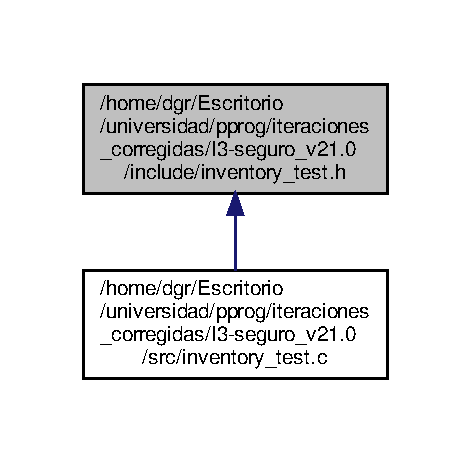
\includegraphics[width=226pt]{inventory__test_8h__dep__incl}
\end{center}
\end{figure}
\subsection*{Functions}
\begin{DoxyCompactItemize}
\item 
void \hyperlink{inventory__test_8h_a33638f1a88ae16ab8d6bee00145b82b8}{test1\+\_\+inventory\+\_\+create} ()
\item 
void \hyperlink{inventory__test_8h_a73a6080c360a8870c4ffc734e989c8b3}{test2\+\_\+inventory\+\_\+create} ()
\item 
void \hyperlink{inventory__test_8h_ad8c004bf0a89d5559e5135a0e0096734}{test1\+\_\+inventory\+\_\+get\+\_\+inside} ()
\item 
void \hyperlink{inventory__test_8h_aa90dc9b98c6d00cbb1fd8be85f9be762}{test2\+\_\+inventory\+\_\+get\+\_\+inside} ()
\item 
void \hyperlink{inventory__test_8h_ae81ec4669af03331ca8a228567736474}{test1\+\_\+inventory\+\_\+add} ()
\item 
void \hyperlink{inventory__test_8h_a48019cb45cb5918233d5d42334d2be17}{test2\+\_\+inventory\+\_\+add} ()
\item 
void \hyperlink{inventory__test_8h_ada5ad194dfe9af537c6b2805bf38910d}{test3\+\_\+inventory\+\_\+add} ()
\item 
void \hyperlink{inventory__test_8h_ac67b0f65fccde3f078e6df452e21cee5}{test1\+\_\+inventory\+\_\+dell} ()
\item 
void \hyperlink{inventory__test_8h_ac0175a02211c4bb5ecffbb9f0ebd1152}{test2\+\_\+inventory\+\_\+dell} ()
\item 
void \hyperlink{inventory__test_8h_a030d6ca8db55a616fe0804b3d0c0c144}{test3\+\_\+inventory\+\_\+dell} ()
\item 
void \hyperlink{inventory__test_8h_a19a0bada9e0ce0def239c2b9523ccfea}{test1\+\_\+inventory\+\_\+is\+\_\+object} ()
\item 
void \hyperlink{inventory__test_8h_a7dc6f9e65941e8cf9b6a983a0de7fc5a}{test2\+\_\+inventory\+\_\+is\+\_\+object} ()
\item 
void \hyperlink{inventory__test_8h_a3adf29b420e3d91803c1dd71f374b468}{test3\+\_\+inventory\+\_\+is\+\_\+object} ()
\item 
void \hyperlink{inventory__test_8h_a257dbc0f18af4e4f73163014faa0783a}{test4\+\_\+inventory\+\_\+is\+\_\+object} ()
\item 
void \hyperlink{inventory__test_8h_a17c03f02b989bb00b04155c12fe2af9d}{test1\+\_\+inventory\+\_\+get\+\_\+max} ()
\item 
void \hyperlink{inventory__test_8h_abddcab377edb21235d6746668597fde2}{test2\+\_\+inventory\+\_\+get\+\_\+max} ()
\item 
void \hyperlink{inventory__test_8h_a7eb3ba387e33c42ff45331c9d9aada34}{test1\+\_\+inventory\+\_\+is\+\_\+full} ()
\item 
void \hyperlink{inventory__test_8h_a1c9e567d4919d5aaccc9580815a8a81d}{test2\+\_\+inventory\+\_\+is\+\_\+full} ()
\item 
void \hyperlink{inventory__test_8h_a540dbcbfd29bd63590d081e496f8227f}{test3\+\_\+inventory\+\_\+is\+\_\+full} ()
\item 
void \hyperlink{inventory__test_8h_a0bfdf05239ed2dbac84e7c1240d27de3}{test1\+\_\+inventory\+\_\+is\+\_\+emty} ()
\item 
void \hyperlink{inventory__test_8h_a00a4e952d7b94aedfdac9bb07ec53b0a}{test2\+\_\+inventory\+\_\+is\+\_\+emty} ()
\item 
void \hyperlink{inventory__test_8h_a8cf624674fe17e81eedcb5801f106016}{test3\+\_\+inventory\+\_\+is\+\_\+emty} ()
\item 
void \hyperlink{inventory__test_8h_ab9578e8992c9afab849de87a6f5e637a}{test1\+\_\+inventory\+\_\+get\+\_\+id} ()
\item 
void \hyperlink{inventory__test_8h_ae39f02e7d91f78fabb2faaa4c3b4f7a7}{test2\+\_\+inventory\+\_\+get\+\_\+id} ()
\end{DoxyCompactItemize}


\subsection{Detailed Description}
It declares the tests for the inventory module. 

\begin{DoxyAuthor}{Author}
Daniel Cerrato Sánchez 
\end{DoxyAuthor}
\begin{DoxyVersion}{Version}
1.\+0 
\end{DoxyVersion}
\begin{DoxyDate}{Date}
10-\/06-\/2020 
\end{DoxyDate}
\begin{DoxyCopyright}{Copyright}
G\+NU Public License 
\end{DoxyCopyright}


\subsection{Function Documentation}
\mbox{\Hypertarget{inventory__test_8h_ae81ec4669af03331ca8a228567736474}\label{inventory__test_8h_ae81ec4669af03331ca8a228567736474}} 
\index{inventory\+\_\+test.\+h@{inventory\+\_\+test.\+h}!test1\+\_\+inventory\+\_\+add@{test1\+\_\+inventory\+\_\+add}}
\index{test1\+\_\+inventory\+\_\+add@{test1\+\_\+inventory\+\_\+add}!inventory\+\_\+test.\+h@{inventory\+\_\+test.\+h}}
\subsubsection{\texorpdfstring{test1\+\_\+inventory\+\_\+add()}{test1\_inventory\_add()}}
{\footnotesize\ttfamily void test1\+\_\+inventory\+\_\+add (\begin{DoxyParamCaption}{ }\end{DoxyParamCaption})}

\begin{DoxyRefDesc}{Test}
\item[\hyperlink{test__test000061}{Test}]Test the function to add objects to an inventory \end{DoxyRefDesc}
\begin{DoxyPrecond}{Precondition}
Inventory is a non-\/\+N\+U\+LL pointer, object id is correct 
\end{DoxyPrecond}
\begin{DoxyPostcond}{Postcondition}
The output must be OK 
\end{DoxyPostcond}
\mbox{\Hypertarget{inventory__test_8h_a33638f1a88ae16ab8d6bee00145b82b8}\label{inventory__test_8h_a33638f1a88ae16ab8d6bee00145b82b8}} 
\index{inventory\+\_\+test.\+h@{inventory\+\_\+test.\+h}!test1\+\_\+inventory\+\_\+create@{test1\+\_\+inventory\+\_\+create}}
\index{test1\+\_\+inventory\+\_\+create@{test1\+\_\+inventory\+\_\+create}!inventory\+\_\+test.\+h@{inventory\+\_\+test.\+h}}
\subsubsection{\texorpdfstring{test1\+\_\+inventory\+\_\+create()}{test1\_inventory\_create()}}
{\footnotesize\ttfamily void test1\+\_\+inventory\+\_\+create (\begin{DoxyParamCaption}{ }\end{DoxyParamCaption})}

\begin{DoxyRefDesc}{Test}
\item[\hyperlink{test__test000057}{Test}]Test the inventory creation function \end{DoxyRefDesc}
\begin{DoxyPrecond}{Precondition}
An id and a maximum of integer objects as parameters 
\end{DoxyPrecond}
\begin{DoxyPostcond}{Postcondition}
A non-\/null pointer to the created inventory 
\end{DoxyPostcond}
\mbox{\Hypertarget{inventory__test_8h_ac67b0f65fccde3f078e6df452e21cee5}\label{inventory__test_8h_ac67b0f65fccde3f078e6df452e21cee5}} 
\index{inventory\+\_\+test.\+h@{inventory\+\_\+test.\+h}!test1\+\_\+inventory\+\_\+dell@{test1\+\_\+inventory\+\_\+dell}}
\index{test1\+\_\+inventory\+\_\+dell@{test1\+\_\+inventory\+\_\+dell}!inventory\+\_\+test.\+h@{inventory\+\_\+test.\+h}}
\subsubsection{\texorpdfstring{test1\+\_\+inventory\+\_\+dell()}{test1\_inventory\_dell()}}
{\footnotesize\ttfamily void test1\+\_\+inventory\+\_\+dell (\begin{DoxyParamCaption}{ }\end{DoxyParamCaption})}

\begin{DoxyRefDesc}{Test}
\item[\hyperlink{test__test000064}{Test}]Test the function to remove objects from an inventory \end{DoxyRefDesc}
\begin{DoxyPrecond}{Precondition}
Inventory is a non-\/\+N\+U\+LL pointer with correct object ids, correct object is searched 
\end{DoxyPrecond}
\begin{DoxyPostcond}{Postcondition}
The output must be OK 
\end{DoxyPostcond}
\mbox{\Hypertarget{inventory__test_8h_ab9578e8992c9afab849de87a6f5e637a}\label{inventory__test_8h_ab9578e8992c9afab849de87a6f5e637a}} 
\index{inventory\+\_\+test.\+h@{inventory\+\_\+test.\+h}!test1\+\_\+inventory\+\_\+get\+\_\+id@{test1\+\_\+inventory\+\_\+get\+\_\+id}}
\index{test1\+\_\+inventory\+\_\+get\+\_\+id@{test1\+\_\+inventory\+\_\+get\+\_\+id}!inventory\+\_\+test.\+h@{inventory\+\_\+test.\+h}}
\subsubsection{\texorpdfstring{test1\+\_\+inventory\+\_\+get\+\_\+id()}{test1\_inventory\_get\_id()}}
{\footnotesize\ttfamily void test1\+\_\+inventory\+\_\+get\+\_\+id (\begin{DoxyParamCaption}{ }\end{DoxyParamCaption})}

\begin{DoxyRefDesc}{Test}
\item[\hyperlink{test__test000079}{Test}]Test the function to get the id of an inventory \end{DoxyRefDesc}
\begin{DoxyPrecond}{Precondition}
Inventory is a non-\/\+N\+U\+LL pointer with correct id 
\end{DoxyPrecond}
\begin{DoxyPostcond}{Postcondition}
The inventory id must be the one entered when creating it 
\end{DoxyPostcond}
\mbox{\Hypertarget{inventory__test_8h_ad8c004bf0a89d5559e5135a0e0096734}\label{inventory__test_8h_ad8c004bf0a89d5559e5135a0e0096734}} 
\index{inventory\+\_\+test.\+h@{inventory\+\_\+test.\+h}!test1\+\_\+inventory\+\_\+get\+\_\+inside@{test1\+\_\+inventory\+\_\+get\+\_\+inside}}
\index{test1\+\_\+inventory\+\_\+get\+\_\+inside@{test1\+\_\+inventory\+\_\+get\+\_\+inside}!inventory\+\_\+test.\+h@{inventory\+\_\+test.\+h}}
\subsubsection{\texorpdfstring{test1\+\_\+inventory\+\_\+get\+\_\+inside()}{test1\_inventory\_get\_inside()}}
{\footnotesize\ttfamily void test1\+\_\+inventory\+\_\+get\+\_\+inside (\begin{DoxyParamCaption}{ }\end{DoxyParamCaption})}

\begin{DoxyRefDesc}{Test}
\item[\hyperlink{test__test000059}{Test}]Test the function to get the inventory item set \end{DoxyRefDesc}
\begin{DoxyPrecond}{Precondition}
Inventory is a non-\/\+N\+U\+LL pointer with correct set 
\end{DoxyPrecond}
\begin{DoxyPostcond}{Postcondition}
The output must be a set as a non-\/\+N\+U\+LL pointer 
\end{DoxyPostcond}
\mbox{\Hypertarget{inventory__test_8h_a17c03f02b989bb00b04155c12fe2af9d}\label{inventory__test_8h_a17c03f02b989bb00b04155c12fe2af9d}} 
\index{inventory\+\_\+test.\+h@{inventory\+\_\+test.\+h}!test1\+\_\+inventory\+\_\+get\+\_\+max@{test1\+\_\+inventory\+\_\+get\+\_\+max}}
\index{test1\+\_\+inventory\+\_\+get\+\_\+max@{test1\+\_\+inventory\+\_\+get\+\_\+max}!inventory\+\_\+test.\+h@{inventory\+\_\+test.\+h}}
\subsubsection{\texorpdfstring{test1\+\_\+inventory\+\_\+get\+\_\+max()}{test1\_inventory\_get\_max()}}
{\footnotesize\ttfamily void test1\+\_\+inventory\+\_\+get\+\_\+max (\begin{DoxyParamCaption}{ }\end{DoxyParamCaption})}

\begin{DoxyRefDesc}{Test}
\item[\hyperlink{test__test000071}{Test}]Test the function to get the maximum number of objects in an inventory \end{DoxyRefDesc}
\begin{DoxyPrecond}{Precondition}
Inventory is a non-\/\+N\+U\+LL pointer with correct maximum 
\end{DoxyPrecond}
\begin{DoxyPostcond}{Postcondition}
The maximum inventory must be the one entered when creating it 
\end{DoxyPostcond}
\mbox{\Hypertarget{inventory__test_8h_a0bfdf05239ed2dbac84e7c1240d27de3}\label{inventory__test_8h_a0bfdf05239ed2dbac84e7c1240d27de3}} 
\index{inventory\+\_\+test.\+h@{inventory\+\_\+test.\+h}!test1\+\_\+inventory\+\_\+is\+\_\+emty@{test1\+\_\+inventory\+\_\+is\+\_\+emty}}
\index{test1\+\_\+inventory\+\_\+is\+\_\+emty@{test1\+\_\+inventory\+\_\+is\+\_\+emty}!inventory\+\_\+test.\+h@{inventory\+\_\+test.\+h}}
\subsubsection{\texorpdfstring{test1\+\_\+inventory\+\_\+is\+\_\+emty()}{test1\_inventory\_is\_emty()}}
{\footnotesize\ttfamily void test1\+\_\+inventory\+\_\+is\+\_\+emty (\begin{DoxyParamCaption}{ }\end{DoxyParamCaption})}

\begin{DoxyRefDesc}{Test}
\item[\hyperlink{test__test000076}{Test}]Test the function to know if an inventory is empty \end{DoxyRefDesc}
\begin{DoxyPrecond}{Precondition}
Inventory is a non-\/\+N\+U\+LL pointer, inventory is empty 
\end{DoxyPrecond}
\begin{DoxyPostcond}{Postcondition}
The output must be T\+R\+UE 
\end{DoxyPostcond}
\mbox{\Hypertarget{inventory__test_8h_a7eb3ba387e33c42ff45331c9d9aada34}\label{inventory__test_8h_a7eb3ba387e33c42ff45331c9d9aada34}} 
\index{inventory\+\_\+test.\+h@{inventory\+\_\+test.\+h}!test1\+\_\+inventory\+\_\+is\+\_\+full@{test1\+\_\+inventory\+\_\+is\+\_\+full}}
\index{test1\+\_\+inventory\+\_\+is\+\_\+full@{test1\+\_\+inventory\+\_\+is\+\_\+full}!inventory\+\_\+test.\+h@{inventory\+\_\+test.\+h}}
\subsubsection{\texorpdfstring{test1\+\_\+inventory\+\_\+is\+\_\+full()}{test1\_inventory\_is\_full()}}
{\footnotesize\ttfamily void test1\+\_\+inventory\+\_\+is\+\_\+full (\begin{DoxyParamCaption}{ }\end{DoxyParamCaption})}

\begin{DoxyRefDesc}{Test}
\item[\hyperlink{test__test000073}{Test}]Test the function to know if an inventory is full \end{DoxyRefDesc}
\begin{DoxyPrecond}{Precondition}
Inventory is a non-\/\+N\+U\+LL pointer, inventory is full 
\end{DoxyPrecond}
\begin{DoxyPostcond}{Postcondition}
The output must be T\+R\+UE 
\end{DoxyPostcond}
\mbox{\Hypertarget{inventory__test_8h_a19a0bada9e0ce0def239c2b9523ccfea}\label{inventory__test_8h_a19a0bada9e0ce0def239c2b9523ccfea}} 
\index{inventory\+\_\+test.\+h@{inventory\+\_\+test.\+h}!test1\+\_\+inventory\+\_\+is\+\_\+object@{test1\+\_\+inventory\+\_\+is\+\_\+object}}
\index{test1\+\_\+inventory\+\_\+is\+\_\+object@{test1\+\_\+inventory\+\_\+is\+\_\+object}!inventory\+\_\+test.\+h@{inventory\+\_\+test.\+h}}
\subsubsection{\texorpdfstring{test1\+\_\+inventory\+\_\+is\+\_\+object()}{test1\_inventory\_is\_object()}}
{\footnotesize\ttfamily void test1\+\_\+inventory\+\_\+is\+\_\+object (\begin{DoxyParamCaption}{ }\end{DoxyParamCaption})}

\begin{DoxyRefDesc}{Test}
\item[\hyperlink{test__test000067}{Test}]Test the function to know if an object is in an inventory \end{DoxyRefDesc}
\begin{DoxyPrecond}{Precondition}
Inventory is a non-\/\+N\+U\+LL pointer to an object, a correct object is searched 
\end{DoxyPrecond}
\begin{DoxyPostcond}{Postcondition}
The output must be T\+R\+UE 
\end{DoxyPostcond}
\mbox{\Hypertarget{inventory__test_8h_a48019cb45cb5918233d5d42334d2be17}\label{inventory__test_8h_a48019cb45cb5918233d5d42334d2be17}} 
\index{inventory\+\_\+test.\+h@{inventory\+\_\+test.\+h}!test2\+\_\+inventory\+\_\+add@{test2\+\_\+inventory\+\_\+add}}
\index{test2\+\_\+inventory\+\_\+add@{test2\+\_\+inventory\+\_\+add}!inventory\+\_\+test.\+h@{inventory\+\_\+test.\+h}}
\subsubsection{\texorpdfstring{test2\+\_\+inventory\+\_\+add()}{test2\_inventory\_add()}}
{\footnotesize\ttfamily void test2\+\_\+inventory\+\_\+add (\begin{DoxyParamCaption}{ }\end{DoxyParamCaption})}

\begin{DoxyRefDesc}{Test}
\item[\hyperlink{test__test000062}{Test}]Test the function to add objects to an inventory \end{DoxyRefDesc}
\begin{DoxyPrecond}{Precondition}
Inventory is a non-\/\+N\+U\+LL pointer, object id is wrong 
\end{DoxyPrecond}
\begin{DoxyPostcond}{Postcondition}
The output must be E\+R\+R\+OR 
\end{DoxyPostcond}
\mbox{\Hypertarget{inventory__test_8h_a73a6080c360a8870c4ffc734e989c8b3}\label{inventory__test_8h_a73a6080c360a8870c4ffc734e989c8b3}} 
\index{inventory\+\_\+test.\+h@{inventory\+\_\+test.\+h}!test2\+\_\+inventory\+\_\+create@{test2\+\_\+inventory\+\_\+create}}
\index{test2\+\_\+inventory\+\_\+create@{test2\+\_\+inventory\+\_\+create}!inventory\+\_\+test.\+h@{inventory\+\_\+test.\+h}}
\subsubsection{\texorpdfstring{test2\+\_\+inventory\+\_\+create()}{test2\_inventory\_create()}}
{\footnotesize\ttfamily void test2\+\_\+inventory\+\_\+create (\begin{DoxyParamCaption}{ }\end{DoxyParamCaption})}

\begin{DoxyRefDesc}{Test}
\item[\hyperlink{test__test000058}{Test}]Test the inventory creation function \end{DoxyRefDesc}
\begin{DoxyPrecond}{Precondition}
Inventory is a non-\/\+N\+U\+LL pointer with correct id 
\end{DoxyPrecond}
\begin{DoxyPostcond}{Postcondition}
The inventory id must be the one entered when creating it 
\end{DoxyPostcond}
\mbox{\Hypertarget{inventory__test_8h_ac0175a02211c4bb5ecffbb9f0ebd1152}\label{inventory__test_8h_ac0175a02211c4bb5ecffbb9f0ebd1152}} 
\index{inventory\+\_\+test.\+h@{inventory\+\_\+test.\+h}!test2\+\_\+inventory\+\_\+dell@{test2\+\_\+inventory\+\_\+dell}}
\index{test2\+\_\+inventory\+\_\+dell@{test2\+\_\+inventory\+\_\+dell}!inventory\+\_\+test.\+h@{inventory\+\_\+test.\+h}}
\subsubsection{\texorpdfstring{test2\+\_\+inventory\+\_\+dell()}{test2\_inventory\_dell()}}
{\footnotesize\ttfamily void test2\+\_\+inventory\+\_\+dell (\begin{DoxyParamCaption}{ }\end{DoxyParamCaption})}

\begin{DoxyRefDesc}{Test}
\item[\hyperlink{test__test000065}{Test}]Test the function to remove objects from an inventory \end{DoxyRefDesc}
\begin{DoxyPrecond}{Precondition}
Inventory is a non-\/\+N\+U\+LL pointer with no object ids 
\end{DoxyPrecond}
\begin{DoxyPostcond}{Postcondition}
The output must be E\+R\+R\+OR 
\end{DoxyPostcond}
\mbox{\Hypertarget{inventory__test_8h_ae39f02e7d91f78fabb2faaa4c3b4f7a7}\label{inventory__test_8h_ae39f02e7d91f78fabb2faaa4c3b4f7a7}} 
\index{inventory\+\_\+test.\+h@{inventory\+\_\+test.\+h}!test2\+\_\+inventory\+\_\+get\+\_\+id@{test2\+\_\+inventory\+\_\+get\+\_\+id}}
\index{test2\+\_\+inventory\+\_\+get\+\_\+id@{test2\+\_\+inventory\+\_\+get\+\_\+id}!inventory\+\_\+test.\+h@{inventory\+\_\+test.\+h}}
\subsubsection{\texorpdfstring{test2\+\_\+inventory\+\_\+get\+\_\+id()}{test2\_inventory\_get\_id()}}
{\footnotesize\ttfamily void test2\+\_\+inventory\+\_\+get\+\_\+id (\begin{DoxyParamCaption}{ }\end{DoxyParamCaption})}

\begin{DoxyRefDesc}{Test}
\item[\hyperlink{test__test000080}{Test}]Test the function to get the id of an inventory \end{DoxyRefDesc}
\begin{DoxyPrecond}{Precondition}
Inventory is a pointer to N\+U\+LL 
\end{DoxyPrecond}
\begin{DoxyPostcond}{Postcondition}
The output must be N\+O\+\_\+\+ID 
\end{DoxyPostcond}
\mbox{\Hypertarget{inventory__test_8h_aa90dc9b98c6d00cbb1fd8be85f9be762}\label{inventory__test_8h_aa90dc9b98c6d00cbb1fd8be85f9be762}} 
\index{inventory\+\_\+test.\+h@{inventory\+\_\+test.\+h}!test2\+\_\+inventory\+\_\+get\+\_\+inside@{test2\+\_\+inventory\+\_\+get\+\_\+inside}}
\index{test2\+\_\+inventory\+\_\+get\+\_\+inside@{test2\+\_\+inventory\+\_\+get\+\_\+inside}!inventory\+\_\+test.\+h@{inventory\+\_\+test.\+h}}
\subsubsection{\texorpdfstring{test2\+\_\+inventory\+\_\+get\+\_\+inside()}{test2\_inventory\_get\_inside()}}
{\footnotesize\ttfamily void test2\+\_\+inventory\+\_\+get\+\_\+inside (\begin{DoxyParamCaption}{ }\end{DoxyParamCaption})}

\begin{DoxyRefDesc}{Test}
\item[\hyperlink{test__test000060}{Test}]Test the function to get the inventory item set \end{DoxyRefDesc}
\begin{DoxyPrecond}{Precondition}
Inventory is a pointer to N\+U\+LL 
\end{DoxyPrecond}
\begin{DoxyPostcond}{Postcondition}
The output must be a set as a pointer to N\+U\+LL 
\end{DoxyPostcond}
\mbox{\Hypertarget{inventory__test_8h_abddcab377edb21235d6746668597fde2}\label{inventory__test_8h_abddcab377edb21235d6746668597fde2}} 
\index{inventory\+\_\+test.\+h@{inventory\+\_\+test.\+h}!test2\+\_\+inventory\+\_\+get\+\_\+max@{test2\+\_\+inventory\+\_\+get\+\_\+max}}
\index{test2\+\_\+inventory\+\_\+get\+\_\+max@{test2\+\_\+inventory\+\_\+get\+\_\+max}!inventory\+\_\+test.\+h@{inventory\+\_\+test.\+h}}
\subsubsection{\texorpdfstring{test2\+\_\+inventory\+\_\+get\+\_\+max()}{test2\_inventory\_get\_max()}}
{\footnotesize\ttfamily void test2\+\_\+inventory\+\_\+get\+\_\+max (\begin{DoxyParamCaption}{ }\end{DoxyParamCaption})}

\begin{DoxyRefDesc}{Test}
\item[\hyperlink{test__test000072}{Test}]Test the function to get the maximum number of objects in an inventory \end{DoxyRefDesc}
\begin{DoxyPrecond}{Precondition}
Inventory is a pointer to N\+U\+LL 
\end{DoxyPrecond}
\begin{DoxyPostcond}{Postcondition}
The output must be -\/1 
\end{DoxyPostcond}
\mbox{\Hypertarget{inventory__test_8h_a00a4e952d7b94aedfdac9bb07ec53b0a}\label{inventory__test_8h_a00a4e952d7b94aedfdac9bb07ec53b0a}} 
\index{inventory\+\_\+test.\+h@{inventory\+\_\+test.\+h}!test2\+\_\+inventory\+\_\+is\+\_\+emty@{test2\+\_\+inventory\+\_\+is\+\_\+emty}}
\index{test2\+\_\+inventory\+\_\+is\+\_\+emty@{test2\+\_\+inventory\+\_\+is\+\_\+emty}!inventory\+\_\+test.\+h@{inventory\+\_\+test.\+h}}
\subsubsection{\texorpdfstring{test2\+\_\+inventory\+\_\+is\+\_\+emty()}{test2\_inventory\_is\_emty()}}
{\footnotesize\ttfamily void test2\+\_\+inventory\+\_\+is\+\_\+emty (\begin{DoxyParamCaption}{ }\end{DoxyParamCaption})}

\begin{DoxyRefDesc}{Test}
\item[\hyperlink{test__test000077}{Test}]Test the function to know if an inventory is empty \end{DoxyRefDesc}
\begin{DoxyPrecond}{Precondition}
Inventory is a non-\/\+N\+U\+LL pointer, inventory is not empty 
\end{DoxyPrecond}
\begin{DoxyPostcond}{Postcondition}
The output must be F\+A\+L\+SE 
\end{DoxyPostcond}
\mbox{\Hypertarget{inventory__test_8h_a1c9e567d4919d5aaccc9580815a8a81d}\label{inventory__test_8h_a1c9e567d4919d5aaccc9580815a8a81d}} 
\index{inventory\+\_\+test.\+h@{inventory\+\_\+test.\+h}!test2\+\_\+inventory\+\_\+is\+\_\+full@{test2\+\_\+inventory\+\_\+is\+\_\+full}}
\index{test2\+\_\+inventory\+\_\+is\+\_\+full@{test2\+\_\+inventory\+\_\+is\+\_\+full}!inventory\+\_\+test.\+h@{inventory\+\_\+test.\+h}}
\subsubsection{\texorpdfstring{test2\+\_\+inventory\+\_\+is\+\_\+full()}{test2\_inventory\_is\_full()}}
{\footnotesize\ttfamily void test2\+\_\+inventory\+\_\+is\+\_\+full (\begin{DoxyParamCaption}{ }\end{DoxyParamCaption})}

\begin{DoxyRefDesc}{Test}
\item[\hyperlink{test__test000074}{Test}]Test the function to know if an inventory is full \end{DoxyRefDesc}
\begin{DoxyPrecond}{Precondition}
Inventory is a non-\/\+N\+U\+LL pointer, inventory is not full 
\end{DoxyPrecond}
\begin{DoxyPostcond}{Postcondition}
The output must be F\+A\+L\+SE 
\end{DoxyPostcond}
\mbox{\Hypertarget{inventory__test_8h_a7dc6f9e65941e8cf9b6a983a0de7fc5a}\label{inventory__test_8h_a7dc6f9e65941e8cf9b6a983a0de7fc5a}} 
\index{inventory\+\_\+test.\+h@{inventory\+\_\+test.\+h}!test2\+\_\+inventory\+\_\+is\+\_\+object@{test2\+\_\+inventory\+\_\+is\+\_\+object}}
\index{test2\+\_\+inventory\+\_\+is\+\_\+object@{test2\+\_\+inventory\+\_\+is\+\_\+object}!inventory\+\_\+test.\+h@{inventory\+\_\+test.\+h}}
\subsubsection{\texorpdfstring{test2\+\_\+inventory\+\_\+is\+\_\+object()}{test2\_inventory\_is\_object()}}
{\footnotesize\ttfamily void test2\+\_\+inventory\+\_\+is\+\_\+object (\begin{DoxyParamCaption}{ }\end{DoxyParamCaption})}

\begin{DoxyRefDesc}{Test}
\item[\hyperlink{test__test000068}{Test}]Test the function to know if an object is in an inventory \end{DoxyRefDesc}
\begin{DoxyPrecond}{Precondition}
Inventory is a non-\/\+N\+U\+LL pointer with no objects 
\end{DoxyPrecond}
\begin{DoxyPostcond}{Postcondition}
The output must be F\+A\+L\+SE 
\end{DoxyPostcond}
\mbox{\Hypertarget{inventory__test_8h_ada5ad194dfe9af537c6b2805bf38910d}\label{inventory__test_8h_ada5ad194dfe9af537c6b2805bf38910d}} 
\index{inventory\+\_\+test.\+h@{inventory\+\_\+test.\+h}!test3\+\_\+inventory\+\_\+add@{test3\+\_\+inventory\+\_\+add}}
\index{test3\+\_\+inventory\+\_\+add@{test3\+\_\+inventory\+\_\+add}!inventory\+\_\+test.\+h@{inventory\+\_\+test.\+h}}
\subsubsection{\texorpdfstring{test3\+\_\+inventory\+\_\+add()}{test3\_inventory\_add()}}
{\footnotesize\ttfamily void test3\+\_\+inventory\+\_\+add (\begin{DoxyParamCaption}{ }\end{DoxyParamCaption})}

\begin{DoxyRefDesc}{Test}
\item[\hyperlink{test__test000063}{Test}]Test the function to add objects to an inventory \end{DoxyRefDesc}
\begin{DoxyPrecond}{Precondition}
Inventory is a pointer to N\+U\+LL 
\end{DoxyPrecond}
\begin{DoxyPostcond}{Postcondition}
The output must be E\+R\+R\+OR 
\end{DoxyPostcond}
\mbox{\Hypertarget{inventory__test_8h_a030d6ca8db55a616fe0804b3d0c0c144}\label{inventory__test_8h_a030d6ca8db55a616fe0804b3d0c0c144}} 
\index{inventory\+\_\+test.\+h@{inventory\+\_\+test.\+h}!test3\+\_\+inventory\+\_\+dell@{test3\+\_\+inventory\+\_\+dell}}
\index{test3\+\_\+inventory\+\_\+dell@{test3\+\_\+inventory\+\_\+dell}!inventory\+\_\+test.\+h@{inventory\+\_\+test.\+h}}
\subsubsection{\texorpdfstring{test3\+\_\+inventory\+\_\+dell()}{test3\_inventory\_dell()}}
{\footnotesize\ttfamily void test3\+\_\+inventory\+\_\+dell (\begin{DoxyParamCaption}{ }\end{DoxyParamCaption})}

\begin{DoxyRefDesc}{Test}
\item[\hyperlink{test__test000066}{Test}]Test the function to remove objects from an inventory \end{DoxyRefDesc}
\begin{DoxyPrecond}{Precondition}
Inventory is a pointer to N\+U\+LL 
\end{DoxyPrecond}
\begin{DoxyPostcond}{Postcondition}
The output must be E\+R\+R\+OR 
\end{DoxyPostcond}
\mbox{\Hypertarget{inventory__test_8h_a8cf624674fe17e81eedcb5801f106016}\label{inventory__test_8h_a8cf624674fe17e81eedcb5801f106016}} 
\index{inventory\+\_\+test.\+h@{inventory\+\_\+test.\+h}!test3\+\_\+inventory\+\_\+is\+\_\+emty@{test3\+\_\+inventory\+\_\+is\+\_\+emty}}
\index{test3\+\_\+inventory\+\_\+is\+\_\+emty@{test3\+\_\+inventory\+\_\+is\+\_\+emty}!inventory\+\_\+test.\+h@{inventory\+\_\+test.\+h}}
\subsubsection{\texorpdfstring{test3\+\_\+inventory\+\_\+is\+\_\+emty()}{test3\_inventory\_is\_emty()}}
{\footnotesize\ttfamily void test3\+\_\+inventory\+\_\+is\+\_\+emty (\begin{DoxyParamCaption}{ }\end{DoxyParamCaption})}

\begin{DoxyRefDesc}{Test}
\item[\hyperlink{test__test000078}{Test}]Test the function to know if an inventory is empty \end{DoxyRefDesc}
\begin{DoxyPrecond}{Precondition}
Inventory is a pointer to N\+U\+LL 
\end{DoxyPrecond}
\begin{DoxyPostcond}{Postcondition}
The output must be T\+R\+UE 
\end{DoxyPostcond}
\mbox{\Hypertarget{inventory__test_8h_a540dbcbfd29bd63590d081e496f8227f}\label{inventory__test_8h_a540dbcbfd29bd63590d081e496f8227f}} 
\index{inventory\+\_\+test.\+h@{inventory\+\_\+test.\+h}!test3\+\_\+inventory\+\_\+is\+\_\+full@{test3\+\_\+inventory\+\_\+is\+\_\+full}}
\index{test3\+\_\+inventory\+\_\+is\+\_\+full@{test3\+\_\+inventory\+\_\+is\+\_\+full}!inventory\+\_\+test.\+h@{inventory\+\_\+test.\+h}}
\subsubsection{\texorpdfstring{test3\+\_\+inventory\+\_\+is\+\_\+full()}{test3\_inventory\_is\_full()}}
{\footnotesize\ttfamily void test3\+\_\+inventory\+\_\+is\+\_\+full (\begin{DoxyParamCaption}{ }\end{DoxyParamCaption})}

\begin{DoxyRefDesc}{Test}
\item[\hyperlink{test__test000075}{Test}]Test the function to know if an inventory is full \end{DoxyRefDesc}
\begin{DoxyPrecond}{Precondition}
Inventory is a pointer to N\+U\+LL 
\end{DoxyPrecond}
\begin{DoxyPostcond}{Postcondition}
The output must be T\+R\+UE 
\end{DoxyPostcond}
\mbox{\Hypertarget{inventory__test_8h_a3adf29b420e3d91803c1dd71f374b468}\label{inventory__test_8h_a3adf29b420e3d91803c1dd71f374b468}} 
\index{inventory\+\_\+test.\+h@{inventory\+\_\+test.\+h}!test3\+\_\+inventory\+\_\+is\+\_\+object@{test3\+\_\+inventory\+\_\+is\+\_\+object}}
\index{test3\+\_\+inventory\+\_\+is\+\_\+object@{test3\+\_\+inventory\+\_\+is\+\_\+object}!inventory\+\_\+test.\+h@{inventory\+\_\+test.\+h}}
\subsubsection{\texorpdfstring{test3\+\_\+inventory\+\_\+is\+\_\+object()}{test3\_inventory\_is\_object()}}
{\footnotesize\ttfamily void test3\+\_\+inventory\+\_\+is\+\_\+object (\begin{DoxyParamCaption}{ }\end{DoxyParamCaption})}

\begin{DoxyRefDesc}{Test}
\item[\hyperlink{test__test000069}{Test}]Test the function to know if an object is in an inventory \end{DoxyRefDesc}
\begin{DoxyPrecond}{Precondition}
Inventory is a non-\/\+N\+U\+LL pointer to an object, an incorrect object is searched 
\end{DoxyPrecond}
\begin{DoxyPostcond}{Postcondition}
The output must be F\+A\+L\+SE 
\end{DoxyPostcond}
\mbox{\Hypertarget{inventory__test_8h_a257dbc0f18af4e4f73163014faa0783a}\label{inventory__test_8h_a257dbc0f18af4e4f73163014faa0783a}} 
\index{inventory\+\_\+test.\+h@{inventory\+\_\+test.\+h}!test4\+\_\+inventory\+\_\+is\+\_\+object@{test4\+\_\+inventory\+\_\+is\+\_\+object}}
\index{test4\+\_\+inventory\+\_\+is\+\_\+object@{test4\+\_\+inventory\+\_\+is\+\_\+object}!inventory\+\_\+test.\+h@{inventory\+\_\+test.\+h}}
\subsubsection{\texorpdfstring{test4\+\_\+inventory\+\_\+is\+\_\+object()}{test4\_inventory\_is\_object()}}
{\footnotesize\ttfamily void test4\+\_\+inventory\+\_\+is\+\_\+object (\begin{DoxyParamCaption}{ }\end{DoxyParamCaption})}

\begin{DoxyRefDesc}{Test}
\item[\hyperlink{test__test000070}{Test}]Test the function to know if an object is in an inventory \end{DoxyRefDesc}
\begin{DoxyPrecond}{Precondition}
Inventory is a pointer to N\+U\+LL 
\end{DoxyPrecond}
\begin{DoxyPostcond}{Postcondition}
The output must be F\+A\+L\+SE 
\end{DoxyPostcond}

\hypertarget{link_8h}{}\section{include/link.h File Reference}
\label{link_8h}\index{include/link.\+h@{include/link.\+h}}


It defines the link interface for each command.  


{\ttfamily \#include \char`\"{}../include/types.\+h\char`\"{}}\newline
Include dependency graph for link.\+h\+:\nopagebreak
\begin{figure}[H]
\begin{center}
\leavevmode
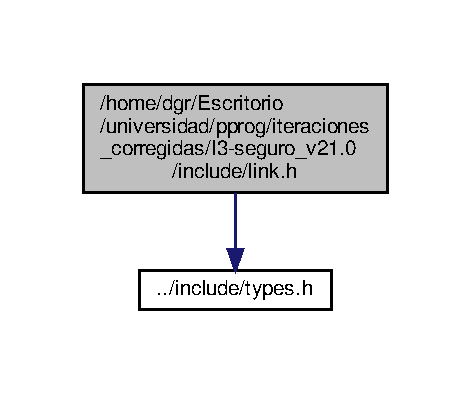
\includegraphics[width=172pt]{link_8h__incl}
\end{center}
\end{figure}
This graph shows which files directly or indirectly include this file\+:\nopagebreak
\begin{figure}[H]
\begin{center}
\leavevmode
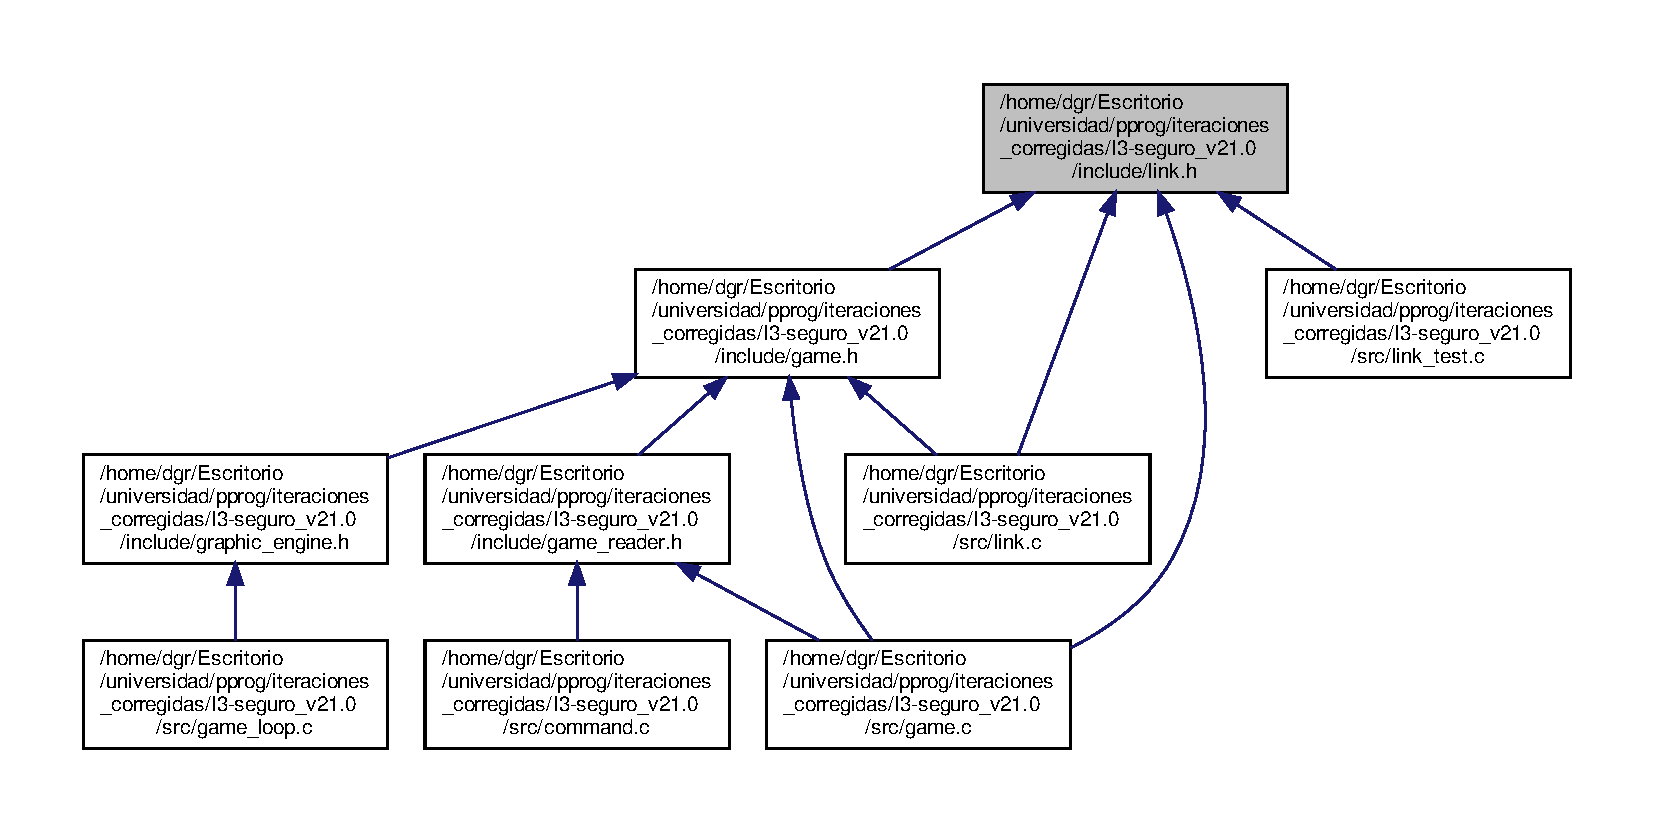
\includegraphics[width=350pt]{link_8h__dep__incl}
\end{center}
\end{figure}
\subsection*{Macros}
\begin{DoxyCompactItemize}
\item 
\#define \hyperlink{link_8h_a660ed1ec8604982002a0d6eced0e0367}{M\+A\+X\+\_\+\+L\+I\+N\+KS}~600
\begin{DoxyCompactList}\small\item\em A macro that stores the maximum links of a game. \end{DoxyCompactList}\end{DoxyCompactItemize}
\subsection*{Typedefs}
\begin{DoxyCompactItemize}
\item 
typedef struct \hyperlink{struct__Link}{\+\_\+\+Link} \hyperlink{link_8h_ae3b299941e67be6971bfd64a25505eff}{Link}
\begin{DoxyCompactList}\small\item\em A type definition for a link. \end{DoxyCompactList}\end{DoxyCompactItemize}
\subsection*{Functions}
\begin{DoxyCompactItemize}
\item 
\hyperlink{link_8h_ae3b299941e67be6971bfd64a25505eff}{Link} $\ast$ \hyperlink{link_8h_a8090d7f529cfd6a2fc5df3dd379fe514}{link\+\_\+create} (\hyperlink{types_8h_a845e604fb28f7e3d97549da3448149d3}{Id} id)
\begin{DoxyCompactList}\small\item\em Create the link, initialite the variables of the link. \end{DoxyCompactList}\item 
\hyperlink{types_8h_a32c27cc471df37f4fc818d65de0a56c4}{S\+T\+A\+T\+US} \hyperlink{link_8h_a6c7a3bd7a856288c377edbcd045912e6}{link\+\_\+set\+\_\+name} (\hyperlink{link_8h_ae3b299941e67be6971bfd64a25505eff}{Link} $\ast$link, char $\ast$name)
\begin{DoxyCompactList}\small\item\em set the name of a link \end{DoxyCompactList}\item 
\hyperlink{types_8h_a32c27cc471df37f4fc818d65de0a56c4}{S\+T\+A\+T\+US} \hyperlink{link_8h_a0f3653e949a03e7cac22d2503f8dc6f4}{link\+\_\+set\+\_\+id1} (\hyperlink{link_8h_ae3b299941e67be6971bfd64a25505eff}{Link} $\ast$link, \hyperlink{types_8h_a845e604fb28f7e3d97549da3448149d3}{Id} id)
\begin{DoxyCompactList}\small\item\em set the origin of a link \end{DoxyCompactList}\item 
\hyperlink{types_8h_a32c27cc471df37f4fc818d65de0a56c4}{S\+T\+A\+T\+US} \hyperlink{link_8h_af3f534402173518ac4fb4880dad3f746}{link\+\_\+set\+\_\+id2} (\hyperlink{link_8h_ae3b299941e67be6971bfd64a25505eff}{Link} $\ast$link, \hyperlink{types_8h_a845e604fb28f7e3d97549da3448149d3}{Id} id)
\begin{DoxyCompactList}\small\item\em set the destination of a link \end{DoxyCompactList}\item 
\hyperlink{types_8h_a32c27cc471df37f4fc818d65de0a56c4}{S\+T\+A\+T\+US} \hyperlink{link_8h_a7e7cd0c8f7c159bf689db53ee87e1bec}{link\+\_\+set\+\_\+open} (\hyperlink{link_8h_ae3b299941e67be6971bfd64a25505eff}{Link} $\ast$link, int open)
\begin{DoxyCompactList}\small\item\em set if the link is closed (1) or open (0) \end{DoxyCompactList}\item 
\hyperlink{types_8h_a32c27cc471df37f4fc818d65de0a56c4}{S\+T\+A\+T\+US} \hyperlink{link_8h_aff9d8ce68a82447a78449fda68f9e755}{link\+\_\+destory} (\hyperlink{link_8h_ae3b299941e67be6971bfd64a25505eff}{Link} $\ast$link)
\begin{DoxyCompactList}\small\item\em destroy a link \end{DoxyCompactList}\item 
\hyperlink{types_8h_a845e604fb28f7e3d97549da3448149d3}{Id} \hyperlink{link_8h_a2bbd320f995a72b2ea7ea639b1c81892}{link\+\_\+get\+\_\+id} (\hyperlink{link_8h_ae3b299941e67be6971bfd64a25505eff}{Link} $\ast$link)
\begin{DoxyCompactList}\small\item\em returns the id of the link that recive \end{DoxyCompactList}\item 
char $\ast$ \hyperlink{link_8h_a9747ee8201a323e112e67bdeacbc90d8}{link\+\_\+get\+\_\+name} (\hyperlink{link_8h_ae3b299941e67be6971bfd64a25505eff}{Link} $\ast$link)
\begin{DoxyCompactList}\small\item\em returns the name of the link that recive \end{DoxyCompactList}\item 
\hyperlink{types_8h_a845e604fb28f7e3d97549da3448149d3}{Id} \hyperlink{link_8h_ad39f5441c13abcb0fce07a81674b04ba}{link\+\_\+get\+\_\+id1} (\hyperlink{link_8h_ae3b299941e67be6971bfd64a25505eff}{Link} $\ast$link)
\begin{DoxyCompactList}\small\item\em returns the origin of the link that recive \end{DoxyCompactList}\item 
\hyperlink{types_8h_a845e604fb28f7e3d97549da3448149d3}{Id} \hyperlink{link_8h_a2079fe643f883e3dcc3c47f9fde4852b}{link\+\_\+get\+\_\+id2} (\hyperlink{link_8h_ae3b299941e67be6971bfd64a25505eff}{Link} $\ast$link)
\begin{DoxyCompactList}\small\item\em returns the destination of the link that recive \end{DoxyCompactList}\item 
\hyperlink{types_8h_a3e5b8192e7d9ffaf3542f1210aec18dd}{B\+O\+OL} \hyperlink{link_8h_a9fab05d77f8cd191a6675ccc6b9d585b}{link\+\_\+is\+\_\+open} (\hyperlink{link_8h_ae3b299941e67be6971bfd64a25505eff}{Link} $\ast$link)
\begin{DoxyCompactList}\small\item\em returns True in case that the link is open, False otherwise \end{DoxyCompactList}\item 
\hyperlink{types_8h_a32c27cc471df37f4fc818d65de0a56c4}{S\+T\+A\+T\+US} \hyperlink{link_8h_a7e0c894d83dbccbf58579b21fd565bb3}{link\+\_\+print} (F\+I\+LE $\ast$f, \hyperlink{link_8h_ae3b299941e67be6971bfd64a25505eff}{Link} $\ast$link)
\begin{DoxyCompactList}\small\item\em prints the information of a link \end{DoxyCompactList}\end{DoxyCompactItemize}


\subsection{Detailed Description}
It defines the link interface for each command. 

\begin{DoxyAuthor}{Author}
David Teófilo Garitagoitia Romero 
\end{DoxyAuthor}
\begin{DoxyVersion}{Version}
1.\+0 
\end{DoxyVersion}
\begin{DoxyDate}{Date}
17-\/03-\/2020 
\end{DoxyDate}
\begin{DoxyCopyright}{Copyright}
G\+NU Public License 
\end{DoxyCopyright}


\subsection{Macro Definition Documentation}
\mbox{\Hypertarget{link_8h_a660ed1ec8604982002a0d6eced0e0367}\label{link_8h_a660ed1ec8604982002a0d6eced0e0367}} 
\index{link.\+h@{link.\+h}!M\+A\+X\+\_\+\+L\+I\+N\+KS@{M\+A\+X\+\_\+\+L\+I\+N\+KS}}
\index{M\+A\+X\+\_\+\+L\+I\+N\+KS@{M\+A\+X\+\_\+\+L\+I\+N\+KS}!link.\+h@{link.\+h}}
\subsubsection{\texorpdfstring{M\+A\+X\+\_\+\+L\+I\+N\+KS}{MAX\_LINKS}}
{\footnotesize\ttfamily \#define M\+A\+X\+\_\+\+L\+I\+N\+KS~600}



A macro that stores the maximum links of a game. 

Details. 

\subsection{Typedef Documentation}
\mbox{\Hypertarget{link_8h_ae3b299941e67be6971bfd64a25505eff}\label{link_8h_ae3b299941e67be6971bfd64a25505eff}} 
\index{link.\+h@{link.\+h}!Link@{Link}}
\index{Link@{Link}!link.\+h@{link.\+h}}
\subsubsection{\texorpdfstring{Link}{Link}}
{\footnotesize\ttfamily typedef struct \hyperlink{struct__Link}{\+\_\+\+Link} \hyperlink{link_8h_ae3b299941e67be6971bfd64a25505eff}{Link}}



A type definition for a link. 

Details. 

\subsection{Function Documentation}
\mbox{\Hypertarget{link_8h_a8090d7f529cfd6a2fc5df3dd379fe514}\label{link_8h_a8090d7f529cfd6a2fc5df3dd379fe514}} 
\index{link.\+h@{link.\+h}!link\+\_\+create@{link\+\_\+create}}
\index{link\+\_\+create@{link\+\_\+create}!link.\+h@{link.\+h}}
\subsubsection{\texorpdfstring{link\+\_\+create()}{link\_create()}}
{\footnotesize\ttfamily \hyperlink{link_8h_ae3b299941e67be6971bfd64a25505eff}{Link}$\ast$ link\+\_\+create (\begin{DoxyParamCaption}\item[{\hyperlink{types_8h_a845e604fb28f7e3d97549da3448149d3}{Id}}]{id }\end{DoxyParamCaption})}



Create the link, initialite the variables of the link. 

link\+\_\+create

\begin{DoxyDate}{Date}
17-\/03-\/2020 
\end{DoxyDate}
\begin{DoxyAuthor}{Author}
David Teófilo Garitagoitia Romero
\end{DoxyAuthor}
\begin{DoxyReturn}{Returns}
the link created 
\end{DoxyReturn}
\mbox{\Hypertarget{link_8h_aff9d8ce68a82447a78449fda68f9e755}\label{link_8h_aff9d8ce68a82447a78449fda68f9e755}} 
\index{link.\+h@{link.\+h}!link\+\_\+destory@{link\+\_\+destory}}
\index{link\+\_\+destory@{link\+\_\+destory}!link.\+h@{link.\+h}}
\subsubsection{\texorpdfstring{link\+\_\+destory()}{link\_destory()}}
{\footnotesize\ttfamily \hyperlink{types_8h_a32c27cc471df37f4fc818d65de0a56c4}{S\+T\+A\+T\+US} link\+\_\+destory (\begin{DoxyParamCaption}\item[{\hyperlink{link_8h_ae3b299941e67be6971bfd64a25505eff}{Link} $\ast$}]{link }\end{DoxyParamCaption})}



destroy a link 

link\+\_\+destroy

\begin{DoxyDate}{Date}
17-\/03-\/2020 
\end{DoxyDate}
\begin{DoxyAuthor}{Author}
David Teófilo Garitagoitia Romero
\end{DoxyAuthor}

\begin{DoxyParams}{Parameters}
{\em link} & the link we want to destroy \\
\hline
\end{DoxyParams}
\begin{DoxyReturn}{Returns}
Ok if there is no error, error otherwise 
\end{DoxyReturn}
\mbox{\Hypertarget{link_8h_a2bbd320f995a72b2ea7ea639b1c81892}\label{link_8h_a2bbd320f995a72b2ea7ea639b1c81892}} 
\index{link.\+h@{link.\+h}!link\+\_\+get\+\_\+id@{link\+\_\+get\+\_\+id}}
\index{link\+\_\+get\+\_\+id@{link\+\_\+get\+\_\+id}!link.\+h@{link.\+h}}
\subsubsection{\texorpdfstring{link\+\_\+get\+\_\+id()}{link\_get\_id()}}
{\footnotesize\ttfamily \hyperlink{types_8h_a845e604fb28f7e3d97549da3448149d3}{Id} link\+\_\+get\+\_\+id (\begin{DoxyParamCaption}\item[{\hyperlink{link_8h_ae3b299941e67be6971bfd64a25505eff}{Link} $\ast$}]{link }\end{DoxyParamCaption})}



returns the id of the link that recive 

link\+\_\+get\+\_\+id

\begin{DoxyDate}{Date}
17-\/03-\/2020 
\end{DoxyDate}
\begin{DoxyAuthor}{Author}
David Teófilo Garitagoitia Romero
\end{DoxyAuthor}

\begin{DoxyParams}{Parameters}
{\em link} & the link of which you want to know their id \\
\hline
\end{DoxyParams}
\begin{DoxyReturn}{Returns}
the id of the link that it recive 
\end{DoxyReturn}
\mbox{\Hypertarget{link_8h_ad39f5441c13abcb0fce07a81674b04ba}\label{link_8h_ad39f5441c13abcb0fce07a81674b04ba}} 
\index{link.\+h@{link.\+h}!link\+\_\+get\+\_\+id1@{link\+\_\+get\+\_\+id1}}
\index{link\+\_\+get\+\_\+id1@{link\+\_\+get\+\_\+id1}!link.\+h@{link.\+h}}
\subsubsection{\texorpdfstring{link\+\_\+get\+\_\+id1()}{link\_get\_id1()}}
{\footnotesize\ttfamily \hyperlink{types_8h_a845e604fb28f7e3d97549da3448149d3}{Id} link\+\_\+get\+\_\+id1 (\begin{DoxyParamCaption}\item[{\hyperlink{link_8h_ae3b299941e67be6971bfd64a25505eff}{Link} $\ast$}]{link }\end{DoxyParamCaption})}



returns the origin of the link that recive 

link\+\_\+get\+\_\+id1

\begin{DoxyDate}{Date}
17-\/03-\/2020 
\end{DoxyDate}
\begin{DoxyAuthor}{Author}
David Teófilo Garitagoitia Romero
\end{DoxyAuthor}

\begin{DoxyParams}{Parameters}
{\em link} & the link of which you want to know their origin \\
\hline
\end{DoxyParams}
\begin{DoxyReturn}{Returns}
the origin of the link that it recives 
\end{DoxyReturn}
\mbox{\Hypertarget{link_8h_a2079fe643f883e3dcc3c47f9fde4852b}\label{link_8h_a2079fe643f883e3dcc3c47f9fde4852b}} 
\index{link.\+h@{link.\+h}!link\+\_\+get\+\_\+id2@{link\+\_\+get\+\_\+id2}}
\index{link\+\_\+get\+\_\+id2@{link\+\_\+get\+\_\+id2}!link.\+h@{link.\+h}}
\subsubsection{\texorpdfstring{link\+\_\+get\+\_\+id2()}{link\_get\_id2()}}
{\footnotesize\ttfamily \hyperlink{types_8h_a845e604fb28f7e3d97549da3448149d3}{Id} link\+\_\+get\+\_\+id2 (\begin{DoxyParamCaption}\item[{\hyperlink{link_8h_ae3b299941e67be6971bfd64a25505eff}{Link} $\ast$}]{link }\end{DoxyParamCaption})}



returns the destination of the link that recive 

link\+\_\+get\+\_\+id2

\begin{DoxyDate}{Date}
17-\/03-\/2020 
\end{DoxyDate}
\begin{DoxyAuthor}{Author}
David Teófilo Garitagoitia Romero
\end{DoxyAuthor}

\begin{DoxyParams}{Parameters}
{\em link} & the link of which you want to know their destination \\
\hline
\end{DoxyParams}
\begin{DoxyReturn}{Returns}
the destination of the link that it recives 
\end{DoxyReturn}
\mbox{\Hypertarget{link_8h_a9747ee8201a323e112e67bdeacbc90d8}\label{link_8h_a9747ee8201a323e112e67bdeacbc90d8}} 
\index{link.\+h@{link.\+h}!link\+\_\+get\+\_\+name@{link\+\_\+get\+\_\+name}}
\index{link\+\_\+get\+\_\+name@{link\+\_\+get\+\_\+name}!link.\+h@{link.\+h}}
\subsubsection{\texorpdfstring{link\+\_\+get\+\_\+name()}{link\_get\_name()}}
{\footnotesize\ttfamily char$\ast$ link\+\_\+get\+\_\+name (\begin{DoxyParamCaption}\item[{\hyperlink{link_8h_ae3b299941e67be6971bfd64a25505eff}{Link} $\ast$}]{link }\end{DoxyParamCaption})}



returns the name of the link that recive 

link\+\_\+get\+\_\+name

\begin{DoxyDate}{Date}
17-\/03-\/2020 
\end{DoxyDate}
\begin{DoxyAuthor}{Author}
David Teófilo Garitagoitia Romero
\end{DoxyAuthor}

\begin{DoxyParams}{Parameters}
{\em link} & the link of which you want to know their name \\
\hline
\end{DoxyParams}
\begin{DoxyReturn}{Returns}
the name of the link that it recives 
\end{DoxyReturn}
\mbox{\Hypertarget{link_8h_a9fab05d77f8cd191a6675ccc6b9d585b}\label{link_8h_a9fab05d77f8cd191a6675ccc6b9d585b}} 
\index{link.\+h@{link.\+h}!link\+\_\+is\+\_\+open@{link\+\_\+is\+\_\+open}}
\index{link\+\_\+is\+\_\+open@{link\+\_\+is\+\_\+open}!link.\+h@{link.\+h}}
\subsubsection{\texorpdfstring{link\+\_\+is\+\_\+open()}{link\_is\_open()}}
{\footnotesize\ttfamily \hyperlink{types_8h_a3e5b8192e7d9ffaf3542f1210aec18dd}{B\+O\+OL} link\+\_\+is\+\_\+open (\begin{DoxyParamCaption}\item[{\hyperlink{link_8h_ae3b299941e67be6971bfd64a25505eff}{Link} $\ast$}]{link }\end{DoxyParamCaption})}



returns True in case that the link is open, False otherwise 

link\+\_\+is\+\_\+open

\begin{DoxyDate}{Date}
17-\/03-\/2020 
\end{DoxyDate}
\begin{DoxyAuthor}{Author}
David Teófilo Garitagoitia Romero
\end{DoxyAuthor}

\begin{DoxyParams}{Parameters}
{\em link} & the link of which you want to know if its open or not \\
\hline
\end{DoxyParams}
\begin{DoxyReturn}{Returns}
True in case that the link is open, False otherwise 
\end{DoxyReturn}
\mbox{\Hypertarget{link_8h_a7e0c894d83dbccbf58579b21fd565bb3}\label{link_8h_a7e0c894d83dbccbf58579b21fd565bb3}} 
\index{link.\+h@{link.\+h}!link\+\_\+print@{link\+\_\+print}}
\index{link\+\_\+print@{link\+\_\+print}!link.\+h@{link.\+h}}
\subsubsection{\texorpdfstring{link\+\_\+print()}{link\_print()}}
{\footnotesize\ttfamily \hyperlink{types_8h_a32c27cc471df37f4fc818d65de0a56c4}{S\+T\+A\+T\+US} link\+\_\+print (\begin{DoxyParamCaption}\item[{F\+I\+LE $\ast$}]{f,  }\item[{\hyperlink{link_8h_ae3b299941e67be6971bfd64a25505eff}{Link} $\ast$}]{link }\end{DoxyParamCaption})}



prints the information of a link 

link\+\_\+print

\begin{DoxyDate}{Date}
17-\/03-\/2020 
\end{DoxyDate}
\begin{DoxyAuthor}{Author}
David Teófilo Garitagoitia Romero
\end{DoxyAuthor}

\begin{DoxyParams}{Parameters}
{\em link} & the link we want to print \\
\hline
{\em f} & the file in which we want to print \\
\hline
\end{DoxyParams}
\begin{DoxyReturn}{Returns}
Ok if there is no error, error otherwise 
\end{DoxyReturn}
\mbox{\Hypertarget{link_8h_a0f3653e949a03e7cac22d2503f8dc6f4}\label{link_8h_a0f3653e949a03e7cac22d2503f8dc6f4}} 
\index{link.\+h@{link.\+h}!link\+\_\+set\+\_\+id1@{link\+\_\+set\+\_\+id1}}
\index{link\+\_\+set\+\_\+id1@{link\+\_\+set\+\_\+id1}!link.\+h@{link.\+h}}
\subsubsection{\texorpdfstring{link\+\_\+set\+\_\+id1()}{link\_set\_id1()}}
{\footnotesize\ttfamily \hyperlink{types_8h_a32c27cc471df37f4fc818d65de0a56c4}{S\+T\+A\+T\+US} link\+\_\+set\+\_\+id1 (\begin{DoxyParamCaption}\item[{\hyperlink{link_8h_ae3b299941e67be6971bfd64a25505eff}{Link} $\ast$}]{link,  }\item[{\hyperlink{types_8h_a845e604fb28f7e3d97549da3448149d3}{Id}}]{id }\end{DoxyParamCaption})}



set the origin of a link 

link\+\_\+set\+\_\+id1

\begin{DoxyDate}{Date}
17-\/03-\/2020 
\end{DoxyDate}
\begin{DoxyAuthor}{Author}
David Teófilo Garitagoitia Romero
\end{DoxyAuthor}

\begin{DoxyParams}{Parameters}
{\em link} & the link in which we want to set the origin \\
\hline
{\em id} & the origin we want to set \\
\hline
\end{DoxyParams}
\begin{DoxyReturn}{Returns}
Ok if there is no error, error otherwise 
\end{DoxyReturn}
\mbox{\Hypertarget{link_8h_af3f534402173518ac4fb4880dad3f746}\label{link_8h_af3f534402173518ac4fb4880dad3f746}} 
\index{link.\+h@{link.\+h}!link\+\_\+set\+\_\+id2@{link\+\_\+set\+\_\+id2}}
\index{link\+\_\+set\+\_\+id2@{link\+\_\+set\+\_\+id2}!link.\+h@{link.\+h}}
\subsubsection{\texorpdfstring{link\+\_\+set\+\_\+id2()}{link\_set\_id2()}}
{\footnotesize\ttfamily \hyperlink{types_8h_a32c27cc471df37f4fc818d65de0a56c4}{S\+T\+A\+T\+US} link\+\_\+set\+\_\+id2 (\begin{DoxyParamCaption}\item[{\hyperlink{link_8h_ae3b299941e67be6971bfd64a25505eff}{Link} $\ast$}]{link,  }\item[{\hyperlink{types_8h_a845e604fb28f7e3d97549da3448149d3}{Id}}]{id }\end{DoxyParamCaption})}



set the destination of a link 

link\+\_\+set\+\_\+id1

\begin{DoxyDate}{Date}
17-\/03-\/2020 
\end{DoxyDate}
\begin{DoxyAuthor}{Author}
David Teófilo Garitagoitia Romero
\end{DoxyAuthor}

\begin{DoxyParams}{Parameters}
{\em link} & the link in which we want to set the destination \\
\hline
{\em id} & the destination we want to set \\
\hline
\end{DoxyParams}
\begin{DoxyReturn}{Returns}
Ok if there is no error, error otherwise 
\end{DoxyReturn}
\mbox{\Hypertarget{link_8h_a6c7a3bd7a856288c377edbcd045912e6}\label{link_8h_a6c7a3bd7a856288c377edbcd045912e6}} 
\index{link.\+h@{link.\+h}!link\+\_\+set\+\_\+name@{link\+\_\+set\+\_\+name}}
\index{link\+\_\+set\+\_\+name@{link\+\_\+set\+\_\+name}!link.\+h@{link.\+h}}
\subsubsection{\texorpdfstring{link\+\_\+set\+\_\+name()}{link\_set\_name()}}
{\footnotesize\ttfamily \hyperlink{types_8h_a32c27cc471df37f4fc818d65de0a56c4}{S\+T\+A\+T\+US} link\+\_\+set\+\_\+name (\begin{DoxyParamCaption}\item[{\hyperlink{link_8h_ae3b299941e67be6971bfd64a25505eff}{Link} $\ast$}]{link,  }\item[{char $\ast$}]{name }\end{DoxyParamCaption})}



set the name of a link 

link\+\_\+set\+\_\+name

\begin{DoxyDate}{Date}
17-\/03-\/2020 
\end{DoxyDate}
\begin{DoxyAuthor}{Author}
David Teófilo Garitagoitia Romero
\end{DoxyAuthor}

\begin{DoxyParams}{Parameters}
{\em link} & the link in which we want to set the name \\
\hline
{\em name} & the name we want to set \\
\hline
\end{DoxyParams}
\begin{DoxyReturn}{Returns}
Ok if there is no error, error otherwise 
\end{DoxyReturn}
\mbox{\Hypertarget{link_8h_a7e7cd0c8f7c159bf689db53ee87e1bec}\label{link_8h_a7e7cd0c8f7c159bf689db53ee87e1bec}} 
\index{link.\+h@{link.\+h}!link\+\_\+set\+\_\+open@{link\+\_\+set\+\_\+open}}
\index{link\+\_\+set\+\_\+open@{link\+\_\+set\+\_\+open}!link.\+h@{link.\+h}}
\subsubsection{\texorpdfstring{link\+\_\+set\+\_\+open()}{link\_set\_open()}}
{\footnotesize\ttfamily \hyperlink{types_8h_a32c27cc471df37f4fc818d65de0a56c4}{S\+T\+A\+T\+US} link\+\_\+set\+\_\+open (\begin{DoxyParamCaption}\item[{\hyperlink{link_8h_ae3b299941e67be6971bfd64a25505eff}{Link} $\ast$}]{link,  }\item[{int}]{open }\end{DoxyParamCaption})}



set if the link is closed (1) or open (0) 

link\+\_\+set\+\_\+open

\begin{DoxyDate}{Date}
17-\/03-\/2020 
\end{DoxyDate}
\begin{DoxyAuthor}{Author}
David Teófilo Garitagoitia Romero
\end{DoxyAuthor}

\begin{DoxyParams}{Parameters}
{\em link} & the link in which we want to set the origin \\
\hline
{\em open} & if the link is open (0), otherwise 1 \\
\hline
\end{DoxyParams}
\begin{DoxyReturn}{Returns}
Ok if there is no error, error otherwise 
\end{DoxyReturn}

\hypertarget{link__test_8h}{}\section{/home/dgr/\+Escritorio/universidad/pprog/iteraciones\+\_\+corregidas/\+I3-\/seguro\+\_\+v21.0/include/link\+\_\+test.h File Reference}
\label{link__test_8h}\index{/home/dgr/\+Escritorio/universidad/pprog/iteraciones\+\_\+corregidas/\+I3-\/seguro\+\_\+v21.\+0/include/link\+\_\+test.\+h@{/home/dgr/\+Escritorio/universidad/pprog/iteraciones\+\_\+corregidas/\+I3-\/seguro\+\_\+v21.\+0/include/link\+\_\+test.\+h}}


It declares the tests for the link module.  


This graph shows which files directly or indirectly include this file\+:
\nopagebreak
\begin{figure}[H]
\begin{center}
\leavevmode
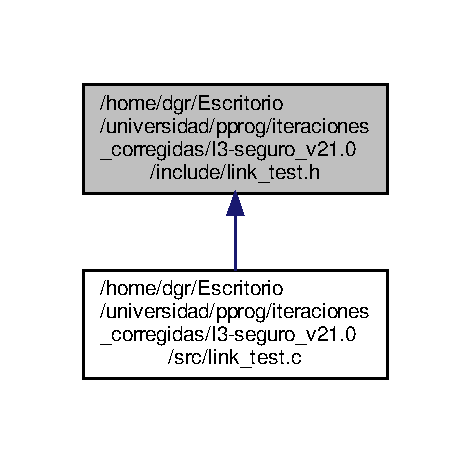
\includegraphics[width=226pt]{link__test_8h__dep__incl}
\end{center}
\end{figure}
\subsection*{Functions}
\begin{DoxyCompactItemize}
\item 
void \hyperlink{link__test_8h_a82c5ee441ad22caad8272212a9e9cc26}{test1\+\_\+link\+\_\+create} ()
\item 
void \hyperlink{link__test_8h_a24b5463da176c3e578b0a0fa8bb1f9f0}{test2\+\_\+link\+\_\+create} ()
\item 
void \hyperlink{link__test_8h_ae0e478a0540bed26befc071591e3ff6c}{test1\+\_\+link\+\_\+set\+\_\+name} ()
\item 
void \hyperlink{link__test_8h_aa66c1e991620a5a758ba6e4d6b4a8b73}{test2\+\_\+link\+\_\+set\+\_\+name} ()
\item 
void \hyperlink{link__test_8h_a42d2fdbe0afa812eb94b9332ab8c3b79}{test1\+\_\+link\+\_\+set\+\_\+id1} ()
\item 
void \hyperlink{link__test_8h_acc401625c94cf6dc9ab66aa974804397}{test2\+\_\+link\+\_\+set\+\_\+id1} ()
\item 
void \hyperlink{link__test_8h_aa4ea6550c6521090364bb423a97724d3}{test1\+\_\+link\+\_\+set\+\_\+id2} ()
\item 
void \hyperlink{link__test_8h_a3a6a81c8b408b2e438884cb3e4d533a3}{test2\+\_\+link\+\_\+set\+\_\+id2} ()
\item 
void \hyperlink{link__test_8h_acbe99eb2aa596b7466ba69d1b78c3f3b}{test1\+\_\+link\+\_\+set\+\_\+open} ()
\item 
void \hyperlink{link__test_8h_a4f7f80db70fdda86df30c5e35c851d65}{test2\+\_\+link\+\_\+set\+\_\+open} ()
\item 
void \hyperlink{link__test_8h_ad4391bca80133c2afaa73a0e520b546e}{test3\+\_\+link\+\_\+set\+\_\+open} ()
\item 
void \hyperlink{link__test_8h_a19c70f79fd51d123173f7aaf6ae50bf8}{test1\+\_\+link\+\_\+get\+\_\+id} ()
\item 
void \hyperlink{link__test_8h_a0f967a1782dd7264e73ad428d22d125d}{test2\+\_\+link\+\_\+get\+\_\+id} ()
\item 
void \hyperlink{link__test_8h_ac3124af4c90d4769cd6e42849817528c}{test1\+\_\+link\+\_\+is\+\_\+open} ()
\item 
void \hyperlink{link__test_8h_a52754541d1357c38da41b0c1b120d5ed}{test2\+\_\+link\+\_\+is\+\_\+open} ()
\item 
void \hyperlink{link__test_8h_a316b5e1d082f5f7133529044b70caaaa}{test3\+\_\+link\+\_\+is\+\_\+open} ()
\item 
void \hyperlink{link__test_8h_ac45f246d7f9b1d21535c743bbb970a85}{test1\+\_\+link\+\_\+get\+\_\+id1} ()
\item 
void \hyperlink{link__test_8h_a26e61cc0a08c97282384a56212168d5a}{test2\+\_\+link\+\_\+get\+\_\+id1} ()
\item 
void \hyperlink{link__test_8h_aeaa87091cae85a91de5db2c755d4eee9}{test1\+\_\+link\+\_\+get\+\_\+id2} ()
\item 
void \hyperlink{link__test_8h_ad9c803361f84a47b5e3f0d475eeb28d0}{test2\+\_\+link\+\_\+get\+\_\+id2} ()
\item 
void \hyperlink{link__test_8h_a044128db00a5cc385d7157dea8bdf3c3}{test1\+\_\+link\+\_\+get\+\_\+name} ()
\item 
void \hyperlink{link__test_8h_a4efc6cfcdc210e2803f9d285734c571e}{test2\+\_\+link\+\_\+get\+\_\+name} ()
\end{DoxyCompactItemize}


\subsection{Detailed Description}
It declares the tests for the link module. 

\begin{DoxyAuthor}{Author}
Daniel Cerrato Sánchez 
\end{DoxyAuthor}
\begin{DoxyVersion}{Version}
1.\+0 
\end{DoxyVersion}
\begin{DoxyDate}{Date}
10-\/06-\/2020 
\end{DoxyDate}
\begin{DoxyCopyright}{Copyright}
G\+NU Public License 
\end{DoxyCopyright}


\subsection{Function Documentation}
\mbox{\Hypertarget{link__test_8h_a82c5ee441ad22caad8272212a9e9cc26}\label{link__test_8h_a82c5ee441ad22caad8272212a9e9cc26}} 
\index{link\+\_\+test.\+h@{link\+\_\+test.\+h}!test1\+\_\+link\+\_\+create@{test1\+\_\+link\+\_\+create}}
\index{test1\+\_\+link\+\_\+create@{test1\+\_\+link\+\_\+create}!link\+\_\+test.\+h@{link\+\_\+test.\+h}}
\subsubsection{\texorpdfstring{test1\+\_\+link\+\_\+create()}{test1\_link\_create()}}
{\footnotesize\ttfamily void test1\+\_\+link\+\_\+create (\begin{DoxyParamCaption}{ }\end{DoxyParamCaption})}

\begin{DoxyRefDesc}{Test}
\item[\hyperlink{test__test000081}{Test}]Test the link creation function \end{DoxyRefDesc}
\begin{DoxyPrecond}{Precondition}
An id as parameter 
\end{DoxyPrecond}
\begin{DoxyPostcond}{Postcondition}
A non-\/null pointer to the created link 
\end{DoxyPostcond}
\mbox{\Hypertarget{link__test_8h_a19c70f79fd51d123173f7aaf6ae50bf8}\label{link__test_8h_a19c70f79fd51d123173f7aaf6ae50bf8}} 
\index{link\+\_\+test.\+h@{link\+\_\+test.\+h}!test1\+\_\+link\+\_\+get\+\_\+id@{test1\+\_\+link\+\_\+get\+\_\+id}}
\index{test1\+\_\+link\+\_\+get\+\_\+id@{test1\+\_\+link\+\_\+get\+\_\+id}!link\+\_\+test.\+h@{link\+\_\+test.\+h}}
\subsubsection{\texorpdfstring{test1\+\_\+link\+\_\+get\+\_\+id()}{test1\_link\_get\_id()}}
{\footnotesize\ttfamily void test1\+\_\+link\+\_\+get\+\_\+id (\begin{DoxyParamCaption}{ }\end{DoxyParamCaption})}

\begin{DoxyRefDesc}{Test}
\item[\hyperlink{test__test000092}{Test}]Test the function to get the id of a link \end{DoxyRefDesc}
\begin{DoxyPrecond}{Precondition}
The link is a non-\/\+N\+U\+LL pointer with correct id 
\end{DoxyPrecond}
\begin{DoxyPostcond}{Postcondition}
The output must be the id entered when creating it 
\end{DoxyPostcond}
\mbox{\Hypertarget{link__test_8h_ac45f246d7f9b1d21535c743bbb970a85}\label{link__test_8h_ac45f246d7f9b1d21535c743bbb970a85}} 
\index{link\+\_\+test.\+h@{link\+\_\+test.\+h}!test1\+\_\+link\+\_\+get\+\_\+id1@{test1\+\_\+link\+\_\+get\+\_\+id1}}
\index{test1\+\_\+link\+\_\+get\+\_\+id1@{test1\+\_\+link\+\_\+get\+\_\+id1}!link\+\_\+test.\+h@{link\+\_\+test.\+h}}
\subsubsection{\texorpdfstring{test1\+\_\+link\+\_\+get\+\_\+id1()}{test1\_link\_get\_id1()}}
{\footnotesize\ttfamily void test1\+\_\+link\+\_\+get\+\_\+id1 (\begin{DoxyParamCaption}{ }\end{DoxyParamCaption})}

\begin{DoxyRefDesc}{Test}
\item[\hyperlink{test__test000097}{Test}]Test the function to get the exit id of a link \end{DoxyRefDesc}
\begin{DoxyPrecond}{Precondition}
The link is a non-\/\+N\+U\+LL pointer with correct exit id 
\end{DoxyPrecond}
\begin{DoxyPostcond}{Postcondition}
The output must be the output id 
\end{DoxyPostcond}
\mbox{\Hypertarget{link__test_8h_aeaa87091cae85a91de5db2c755d4eee9}\label{link__test_8h_aeaa87091cae85a91de5db2c755d4eee9}} 
\index{link\+\_\+test.\+h@{link\+\_\+test.\+h}!test1\+\_\+link\+\_\+get\+\_\+id2@{test1\+\_\+link\+\_\+get\+\_\+id2}}
\index{test1\+\_\+link\+\_\+get\+\_\+id2@{test1\+\_\+link\+\_\+get\+\_\+id2}!link\+\_\+test.\+h@{link\+\_\+test.\+h}}
\subsubsection{\texorpdfstring{test1\+\_\+link\+\_\+get\+\_\+id2()}{test1\_link\_get\_id2()}}
{\footnotesize\ttfamily void test1\+\_\+link\+\_\+get\+\_\+id2 (\begin{DoxyParamCaption}{ }\end{DoxyParamCaption})}

\begin{DoxyRefDesc}{Test}
\item[\hyperlink{test__test000099}{Test}]Test the function to get the input id of a link \end{DoxyRefDesc}
\begin{DoxyPrecond}{Precondition}
The link is a non-\/\+N\+U\+LL pointer with correct input id 
\end{DoxyPrecond}
\begin{DoxyPostcond}{Postcondition}
The output must be the input id 
\end{DoxyPostcond}
\mbox{\Hypertarget{link__test_8h_a044128db00a5cc385d7157dea8bdf3c3}\label{link__test_8h_a044128db00a5cc385d7157dea8bdf3c3}} 
\index{link\+\_\+test.\+h@{link\+\_\+test.\+h}!test1\+\_\+link\+\_\+get\+\_\+name@{test1\+\_\+link\+\_\+get\+\_\+name}}
\index{test1\+\_\+link\+\_\+get\+\_\+name@{test1\+\_\+link\+\_\+get\+\_\+name}!link\+\_\+test.\+h@{link\+\_\+test.\+h}}
\subsubsection{\texorpdfstring{test1\+\_\+link\+\_\+get\+\_\+name()}{test1\_link\_get\_name()}}
{\footnotesize\ttfamily void test1\+\_\+link\+\_\+get\+\_\+name (\begin{DoxyParamCaption}{ }\end{DoxyParamCaption})}

\begin{DoxyRefDesc}{Test}
\item[\hyperlink{test__test000101}{Test}]Test the function to get the name of a link \end{DoxyRefDesc}
\begin{DoxyPrecond}{Precondition}
The link is a non-\/\+N\+U\+LL pointer with correct name 
\end{DoxyPrecond}
\begin{DoxyPostcond}{Postcondition}
The comparison between the name and the word to compare must be 0 
\end{DoxyPostcond}
\mbox{\Hypertarget{link__test_8h_ac3124af4c90d4769cd6e42849817528c}\label{link__test_8h_ac3124af4c90d4769cd6e42849817528c}} 
\index{link\+\_\+test.\+h@{link\+\_\+test.\+h}!test1\+\_\+link\+\_\+is\+\_\+open@{test1\+\_\+link\+\_\+is\+\_\+open}}
\index{test1\+\_\+link\+\_\+is\+\_\+open@{test1\+\_\+link\+\_\+is\+\_\+open}!link\+\_\+test.\+h@{link\+\_\+test.\+h}}
\subsubsection{\texorpdfstring{test1\+\_\+link\+\_\+is\+\_\+open()}{test1\_link\_is\_open()}}
{\footnotesize\ttfamily void test1\+\_\+link\+\_\+is\+\_\+open (\begin{DoxyParamCaption}{ }\end{DoxyParamCaption})}

\begin{DoxyRefDesc}{Test}
\item[\hyperlink{test__test000094}{Test}]Test the function to get the opening status of a link \end{DoxyRefDesc}
\begin{DoxyPrecond}{Precondition}
The link is a non-\/\+N\+U\+LL pointer with status 0 (open) 
\end{DoxyPrecond}
\begin{DoxyPostcond}{Postcondition}
The output must be T\+R\+UE 
\end{DoxyPostcond}
\mbox{\Hypertarget{link__test_8h_a42d2fdbe0afa812eb94b9332ab8c3b79}\label{link__test_8h_a42d2fdbe0afa812eb94b9332ab8c3b79}} 
\index{link\+\_\+test.\+h@{link\+\_\+test.\+h}!test1\+\_\+link\+\_\+set\+\_\+id1@{test1\+\_\+link\+\_\+set\+\_\+id1}}
\index{test1\+\_\+link\+\_\+set\+\_\+id1@{test1\+\_\+link\+\_\+set\+\_\+id1}!link\+\_\+test.\+h@{link\+\_\+test.\+h}}
\subsubsection{\texorpdfstring{test1\+\_\+link\+\_\+set\+\_\+id1()}{test1\_link\_set\_id1()}}
{\footnotesize\ttfamily void test1\+\_\+link\+\_\+set\+\_\+id1 (\begin{DoxyParamCaption}{ }\end{DoxyParamCaption})}

\begin{DoxyRefDesc}{Test}
\item[\hyperlink{test__test000085}{Test}]Test the function to change the exit id of a link \end{DoxyRefDesc}
\begin{DoxyPrecond}{Precondition}
The link is a non-\/\+N\+U\+LL pointer, the exit id is correct 
\end{DoxyPrecond}
\begin{DoxyPostcond}{Postcondition}
The output must be OK 
\end{DoxyPostcond}
\mbox{\Hypertarget{link__test_8h_aa4ea6550c6521090364bb423a97724d3}\label{link__test_8h_aa4ea6550c6521090364bb423a97724d3}} 
\index{link\+\_\+test.\+h@{link\+\_\+test.\+h}!test1\+\_\+link\+\_\+set\+\_\+id2@{test1\+\_\+link\+\_\+set\+\_\+id2}}
\index{test1\+\_\+link\+\_\+set\+\_\+id2@{test1\+\_\+link\+\_\+set\+\_\+id2}!link\+\_\+test.\+h@{link\+\_\+test.\+h}}
\subsubsection{\texorpdfstring{test1\+\_\+link\+\_\+set\+\_\+id2()}{test1\_link\_set\_id2()}}
{\footnotesize\ttfamily void test1\+\_\+link\+\_\+set\+\_\+id2 (\begin{DoxyParamCaption}{ }\end{DoxyParamCaption})}

\begin{DoxyRefDesc}{Test}
\item[\hyperlink{test__test000087}{Test}]Test the function to change the input id of a link \end{DoxyRefDesc}
\begin{DoxyPrecond}{Precondition}
The link is a non-\/\+N\+U\+LL pointer, the input id is correct 
\end{DoxyPrecond}
\begin{DoxyPostcond}{Postcondition}
The output must be OK 
\end{DoxyPostcond}
\mbox{\Hypertarget{link__test_8h_ae0e478a0540bed26befc071591e3ff6c}\label{link__test_8h_ae0e478a0540bed26befc071591e3ff6c}} 
\index{link\+\_\+test.\+h@{link\+\_\+test.\+h}!test1\+\_\+link\+\_\+set\+\_\+name@{test1\+\_\+link\+\_\+set\+\_\+name}}
\index{test1\+\_\+link\+\_\+set\+\_\+name@{test1\+\_\+link\+\_\+set\+\_\+name}!link\+\_\+test.\+h@{link\+\_\+test.\+h}}
\subsubsection{\texorpdfstring{test1\+\_\+link\+\_\+set\+\_\+name()}{test1\_link\_set\_name()}}
{\footnotesize\ttfamily void test1\+\_\+link\+\_\+set\+\_\+name (\begin{DoxyParamCaption}{ }\end{DoxyParamCaption})}

\begin{DoxyRefDesc}{Test}
\item[\hyperlink{test__test000083}{Test}]Test the function to rename a link \end{DoxyRefDesc}
\begin{DoxyPrecond}{Precondition}
The link is a non-\/\+N\+U\+LL pointer, the name is correct 
\end{DoxyPrecond}
\begin{DoxyPostcond}{Postcondition}
The output must be OK 
\end{DoxyPostcond}
\mbox{\Hypertarget{link__test_8h_acbe99eb2aa596b7466ba69d1b78c3f3b}\label{link__test_8h_acbe99eb2aa596b7466ba69d1b78c3f3b}} 
\index{link\+\_\+test.\+h@{link\+\_\+test.\+h}!test1\+\_\+link\+\_\+set\+\_\+open@{test1\+\_\+link\+\_\+set\+\_\+open}}
\index{test1\+\_\+link\+\_\+set\+\_\+open@{test1\+\_\+link\+\_\+set\+\_\+open}!link\+\_\+test.\+h@{link\+\_\+test.\+h}}
\subsubsection{\texorpdfstring{test1\+\_\+link\+\_\+set\+\_\+open()}{test1\_link\_set\_open()}}
{\footnotesize\ttfamily void test1\+\_\+link\+\_\+set\+\_\+open (\begin{DoxyParamCaption}{ }\end{DoxyParamCaption})}

\begin{DoxyRefDesc}{Test}
\item[\hyperlink{test__test000089}{Test}]Test the function to change the opening state of a link \end{DoxyRefDesc}
\begin{DoxyPrecond}{Precondition}
The link is a non-\/\+N\+U\+LL pointer, the state is 0 (open) 
\end{DoxyPrecond}
\begin{DoxyPostcond}{Postcondition}
The output must be OK 
\end{DoxyPostcond}
\mbox{\Hypertarget{link__test_8h_a24b5463da176c3e578b0a0fa8bb1f9f0}\label{link__test_8h_a24b5463da176c3e578b0a0fa8bb1f9f0}} 
\index{link\+\_\+test.\+h@{link\+\_\+test.\+h}!test2\+\_\+link\+\_\+create@{test2\+\_\+link\+\_\+create}}
\index{test2\+\_\+link\+\_\+create@{test2\+\_\+link\+\_\+create}!link\+\_\+test.\+h@{link\+\_\+test.\+h}}
\subsubsection{\texorpdfstring{test2\+\_\+link\+\_\+create()}{test2\_link\_create()}}
{\footnotesize\ttfamily void test2\+\_\+link\+\_\+create (\begin{DoxyParamCaption}{ }\end{DoxyParamCaption})}

\begin{DoxyRefDesc}{Test}
\item[\hyperlink{test__test000082}{Test}]Test the link creation function \end{DoxyRefDesc}
\begin{DoxyPrecond}{Precondition}
The link is a non-\/\+N\+U\+LL pointer with correct id 
\end{DoxyPrecond}
\begin{DoxyPostcond}{Postcondition}
The link id must be the one entered when creating it 
\end{DoxyPostcond}
\mbox{\Hypertarget{link__test_8h_a0f967a1782dd7264e73ad428d22d125d}\label{link__test_8h_a0f967a1782dd7264e73ad428d22d125d}} 
\index{link\+\_\+test.\+h@{link\+\_\+test.\+h}!test2\+\_\+link\+\_\+get\+\_\+id@{test2\+\_\+link\+\_\+get\+\_\+id}}
\index{test2\+\_\+link\+\_\+get\+\_\+id@{test2\+\_\+link\+\_\+get\+\_\+id}!link\+\_\+test.\+h@{link\+\_\+test.\+h}}
\subsubsection{\texorpdfstring{test2\+\_\+link\+\_\+get\+\_\+id()}{test2\_link\_get\_id()}}
{\footnotesize\ttfamily void test2\+\_\+link\+\_\+get\+\_\+id (\begin{DoxyParamCaption}{ }\end{DoxyParamCaption})}

\begin{DoxyRefDesc}{Test}
\item[\hyperlink{test__test000093}{Test}]Test the function to get the id of a link \end{DoxyRefDesc}
\begin{DoxyPrecond}{Precondition}
The link is a pointer to N\+U\+LL 
\end{DoxyPrecond}
\begin{DoxyPostcond}{Postcondition}
The output must be N\+O\+\_\+\+ID 
\end{DoxyPostcond}
\mbox{\Hypertarget{link__test_8h_a26e61cc0a08c97282384a56212168d5a}\label{link__test_8h_a26e61cc0a08c97282384a56212168d5a}} 
\index{link\+\_\+test.\+h@{link\+\_\+test.\+h}!test2\+\_\+link\+\_\+get\+\_\+id1@{test2\+\_\+link\+\_\+get\+\_\+id1}}
\index{test2\+\_\+link\+\_\+get\+\_\+id1@{test2\+\_\+link\+\_\+get\+\_\+id1}!link\+\_\+test.\+h@{link\+\_\+test.\+h}}
\subsubsection{\texorpdfstring{test2\+\_\+link\+\_\+get\+\_\+id1()}{test2\_link\_get\_id1()}}
{\footnotesize\ttfamily void test2\+\_\+link\+\_\+get\+\_\+id1 (\begin{DoxyParamCaption}{ }\end{DoxyParamCaption})}

\begin{DoxyRefDesc}{Test}
\item[\hyperlink{test__test000098}{Test}]Test the function to get the exit id of a link \end{DoxyRefDesc}
\begin{DoxyPrecond}{Precondition}
The link is a pointer to N\+U\+LL 
\end{DoxyPrecond}
\begin{DoxyPostcond}{Postcondition}
The output must be N\+O\+\_\+\+ID 
\end{DoxyPostcond}
\mbox{\Hypertarget{link__test_8h_ad9c803361f84a47b5e3f0d475eeb28d0}\label{link__test_8h_ad9c803361f84a47b5e3f0d475eeb28d0}} 
\index{link\+\_\+test.\+h@{link\+\_\+test.\+h}!test2\+\_\+link\+\_\+get\+\_\+id2@{test2\+\_\+link\+\_\+get\+\_\+id2}}
\index{test2\+\_\+link\+\_\+get\+\_\+id2@{test2\+\_\+link\+\_\+get\+\_\+id2}!link\+\_\+test.\+h@{link\+\_\+test.\+h}}
\subsubsection{\texorpdfstring{test2\+\_\+link\+\_\+get\+\_\+id2()}{test2\_link\_get\_id2()}}
{\footnotesize\ttfamily void test2\+\_\+link\+\_\+get\+\_\+id2 (\begin{DoxyParamCaption}{ }\end{DoxyParamCaption})}

\begin{DoxyRefDesc}{Test}
\item[\hyperlink{test__test000100}{Test}]Test the function to get the input id of a link \end{DoxyRefDesc}
\begin{DoxyPrecond}{Precondition}
The link is a pointer to N\+U\+LL 
\end{DoxyPrecond}
\begin{DoxyPostcond}{Postcondition}
The output must be N\+O\+\_\+\+ID 
\end{DoxyPostcond}
\mbox{\Hypertarget{link__test_8h_a4efc6cfcdc210e2803f9d285734c571e}\label{link__test_8h_a4efc6cfcdc210e2803f9d285734c571e}} 
\index{link\+\_\+test.\+h@{link\+\_\+test.\+h}!test2\+\_\+link\+\_\+get\+\_\+name@{test2\+\_\+link\+\_\+get\+\_\+name}}
\index{test2\+\_\+link\+\_\+get\+\_\+name@{test2\+\_\+link\+\_\+get\+\_\+name}!link\+\_\+test.\+h@{link\+\_\+test.\+h}}
\subsubsection{\texorpdfstring{test2\+\_\+link\+\_\+get\+\_\+name()}{test2\_link\_get\_name()}}
{\footnotesize\ttfamily void test2\+\_\+link\+\_\+get\+\_\+name (\begin{DoxyParamCaption}{ }\end{DoxyParamCaption})}

\begin{DoxyRefDesc}{Test}
\item[\hyperlink{test__test000102}{Test}]Test the function to get the name of a link \end{DoxyRefDesc}
\begin{DoxyPrecond}{Precondition}
The link is a pointer to N\+U\+LL 
\end{DoxyPrecond}
\begin{DoxyPostcond}{Postcondition}
The output must be N\+U\+LL 
\end{DoxyPostcond}
\mbox{\Hypertarget{link__test_8h_a52754541d1357c38da41b0c1b120d5ed}\label{link__test_8h_a52754541d1357c38da41b0c1b120d5ed}} 
\index{link\+\_\+test.\+h@{link\+\_\+test.\+h}!test2\+\_\+link\+\_\+is\+\_\+open@{test2\+\_\+link\+\_\+is\+\_\+open}}
\index{test2\+\_\+link\+\_\+is\+\_\+open@{test2\+\_\+link\+\_\+is\+\_\+open}!link\+\_\+test.\+h@{link\+\_\+test.\+h}}
\subsubsection{\texorpdfstring{test2\+\_\+link\+\_\+is\+\_\+open()}{test2\_link\_is\_open()}}
{\footnotesize\ttfamily void test2\+\_\+link\+\_\+is\+\_\+open (\begin{DoxyParamCaption}{ }\end{DoxyParamCaption})}

\begin{DoxyRefDesc}{Test}
\item[\hyperlink{test__test000095}{Test}]Test the function to get the opening status of a link \end{DoxyRefDesc}
\begin{DoxyPrecond}{Precondition}
The link is a non-\/\+N\+U\+LL pointer with status 1 (closed) 
\end{DoxyPrecond}
\begin{DoxyPostcond}{Postcondition}
The output must be F\+A\+L\+SE 
\end{DoxyPostcond}
\mbox{\Hypertarget{link__test_8h_acc401625c94cf6dc9ab66aa974804397}\label{link__test_8h_acc401625c94cf6dc9ab66aa974804397}} 
\index{link\+\_\+test.\+h@{link\+\_\+test.\+h}!test2\+\_\+link\+\_\+set\+\_\+id1@{test2\+\_\+link\+\_\+set\+\_\+id1}}
\index{test2\+\_\+link\+\_\+set\+\_\+id1@{test2\+\_\+link\+\_\+set\+\_\+id1}!link\+\_\+test.\+h@{link\+\_\+test.\+h}}
\subsubsection{\texorpdfstring{test2\+\_\+link\+\_\+set\+\_\+id1()}{test2\_link\_set\_id1()}}
{\footnotesize\ttfamily void test2\+\_\+link\+\_\+set\+\_\+id1 (\begin{DoxyParamCaption}{ }\end{DoxyParamCaption})}

\begin{DoxyRefDesc}{Test}
\item[\hyperlink{test__test000086}{Test}]Test the function to change the exit id of a link \end{DoxyRefDesc}
\begin{DoxyPrecond}{Precondition}
The link is a pointer to N\+U\+LL 
\end{DoxyPrecond}
\begin{DoxyPostcond}{Postcondition}
The output must be E\+R\+R\+OR 
\end{DoxyPostcond}
\mbox{\Hypertarget{link__test_8h_a3a6a81c8b408b2e438884cb3e4d533a3}\label{link__test_8h_a3a6a81c8b408b2e438884cb3e4d533a3}} 
\index{link\+\_\+test.\+h@{link\+\_\+test.\+h}!test2\+\_\+link\+\_\+set\+\_\+id2@{test2\+\_\+link\+\_\+set\+\_\+id2}}
\index{test2\+\_\+link\+\_\+set\+\_\+id2@{test2\+\_\+link\+\_\+set\+\_\+id2}!link\+\_\+test.\+h@{link\+\_\+test.\+h}}
\subsubsection{\texorpdfstring{test2\+\_\+link\+\_\+set\+\_\+id2()}{test2\_link\_set\_id2()}}
{\footnotesize\ttfamily void test2\+\_\+link\+\_\+set\+\_\+id2 (\begin{DoxyParamCaption}{ }\end{DoxyParamCaption})}

\begin{DoxyRefDesc}{Test}
\item[\hyperlink{test__test000088}{Test}]Test the function to change the input id of a link \end{DoxyRefDesc}
\begin{DoxyPrecond}{Precondition}
The link is a pointer to N\+U\+LL 
\end{DoxyPrecond}
\begin{DoxyPostcond}{Postcondition}
The output must be E\+R\+R\+OR 
\end{DoxyPostcond}
\mbox{\Hypertarget{link__test_8h_aa66c1e991620a5a758ba6e4d6b4a8b73}\label{link__test_8h_aa66c1e991620a5a758ba6e4d6b4a8b73}} 
\index{link\+\_\+test.\+h@{link\+\_\+test.\+h}!test2\+\_\+link\+\_\+set\+\_\+name@{test2\+\_\+link\+\_\+set\+\_\+name}}
\index{test2\+\_\+link\+\_\+set\+\_\+name@{test2\+\_\+link\+\_\+set\+\_\+name}!link\+\_\+test.\+h@{link\+\_\+test.\+h}}
\subsubsection{\texorpdfstring{test2\+\_\+link\+\_\+set\+\_\+name()}{test2\_link\_set\_name()}}
{\footnotesize\ttfamily void test2\+\_\+link\+\_\+set\+\_\+name (\begin{DoxyParamCaption}{ }\end{DoxyParamCaption})}

\begin{DoxyRefDesc}{Test}
\item[\hyperlink{test__test000084}{Test}]Test the function to rename a link \end{DoxyRefDesc}
\begin{DoxyPrecond}{Precondition}
The link is a non-\/\+N\+U\+LL pointer, the name is N\+U\+LL 
\end{DoxyPrecond}
\begin{DoxyPostcond}{Postcondition}
The output must be E\+R\+R\+OR 
\end{DoxyPostcond}
\mbox{\Hypertarget{link__test_8h_a4f7f80db70fdda86df30c5e35c851d65}\label{link__test_8h_a4f7f80db70fdda86df30c5e35c851d65}} 
\index{link\+\_\+test.\+h@{link\+\_\+test.\+h}!test2\+\_\+link\+\_\+set\+\_\+open@{test2\+\_\+link\+\_\+set\+\_\+open}}
\index{test2\+\_\+link\+\_\+set\+\_\+open@{test2\+\_\+link\+\_\+set\+\_\+open}!link\+\_\+test.\+h@{link\+\_\+test.\+h}}
\subsubsection{\texorpdfstring{test2\+\_\+link\+\_\+set\+\_\+open()}{test2\_link\_set\_open()}}
{\footnotesize\ttfamily void test2\+\_\+link\+\_\+set\+\_\+open (\begin{DoxyParamCaption}{ }\end{DoxyParamCaption})}

\begin{DoxyRefDesc}{Test}
\item[\hyperlink{test__test000090}{Test}]Test the function to change the opening state of a link \end{DoxyRefDesc}
\begin{DoxyPrecond}{Precondition}
The link is a non-\/\+N\+U\+LL pointer, the state is 1 (closed) 
\end{DoxyPrecond}
\begin{DoxyPostcond}{Postcondition}
The output must be OK 
\end{DoxyPostcond}
\mbox{\Hypertarget{link__test_8h_a316b5e1d082f5f7133529044b70caaaa}\label{link__test_8h_a316b5e1d082f5f7133529044b70caaaa}} 
\index{link\+\_\+test.\+h@{link\+\_\+test.\+h}!test3\+\_\+link\+\_\+is\+\_\+open@{test3\+\_\+link\+\_\+is\+\_\+open}}
\index{test3\+\_\+link\+\_\+is\+\_\+open@{test3\+\_\+link\+\_\+is\+\_\+open}!link\+\_\+test.\+h@{link\+\_\+test.\+h}}
\subsubsection{\texorpdfstring{test3\+\_\+link\+\_\+is\+\_\+open()}{test3\_link\_is\_open()}}
{\footnotesize\ttfamily void test3\+\_\+link\+\_\+is\+\_\+open (\begin{DoxyParamCaption}{ }\end{DoxyParamCaption})}

\begin{DoxyRefDesc}{Test}
\item[\hyperlink{test__test000096}{Test}]Test the function to get the opening status of a link \end{DoxyRefDesc}
\begin{DoxyPrecond}{Precondition}
The link is a pointer to N\+U\+LL 
\end{DoxyPrecond}
\begin{DoxyPostcond}{Postcondition}
The output must be F\+A\+L\+SE 
\end{DoxyPostcond}
\mbox{\Hypertarget{link__test_8h_ad4391bca80133c2afaa73a0e520b546e}\label{link__test_8h_ad4391bca80133c2afaa73a0e520b546e}} 
\index{link\+\_\+test.\+h@{link\+\_\+test.\+h}!test3\+\_\+link\+\_\+set\+\_\+open@{test3\+\_\+link\+\_\+set\+\_\+open}}
\index{test3\+\_\+link\+\_\+set\+\_\+open@{test3\+\_\+link\+\_\+set\+\_\+open}!link\+\_\+test.\+h@{link\+\_\+test.\+h}}
\subsubsection{\texorpdfstring{test3\+\_\+link\+\_\+set\+\_\+open()}{test3\_link\_set\_open()}}
{\footnotesize\ttfamily void test3\+\_\+link\+\_\+set\+\_\+open (\begin{DoxyParamCaption}{ }\end{DoxyParamCaption})}

\begin{DoxyRefDesc}{Test}
\item[\hyperlink{test__test000091}{Test}]Test the function to change the opening state of a link \end{DoxyRefDesc}
\begin{DoxyPrecond}{Precondition}
The link is a pointer to N\+U\+LL 
\end{DoxyPrecond}
\begin{DoxyPostcond}{Postcondition}
The output must be E\+R\+R\+OR 
\end{DoxyPostcond}

\hypertarget{object_8h}{}\section{/home/dgr/\+Escritorio/universidad/pprog/iteraciones\+\_\+corregidas/\+I3-\/seguro\+\_\+v21.0/include/object.h File Reference}
\label{object_8h}\index{/home/dgr/\+Escritorio/universidad/pprog/iteraciones\+\_\+corregidas/\+I3-\/seguro\+\_\+v21.\+0/include/object.\+h@{/home/dgr/\+Escritorio/universidad/pprog/iteraciones\+\_\+corregidas/\+I3-\/seguro\+\_\+v21.\+0/include/object.\+h}}


It defines the object interface for each command.  


{\ttfamily \#include \char`\"{}../include/types.\+h\char`\"{}}\newline
Include dependency graph for object.\+h\+:
\nopagebreak
\begin{figure}[H]
\begin{center}
\leavevmode
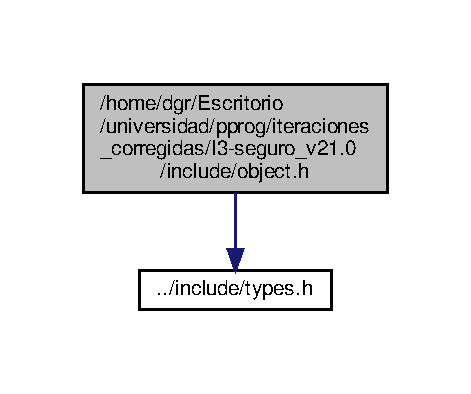
\includegraphics[width=226pt]{object_8h__incl}
\end{center}
\end{figure}
This graph shows which files directly or indirectly include this file\+:
\nopagebreak
\begin{figure}[H]
\begin{center}
\leavevmode
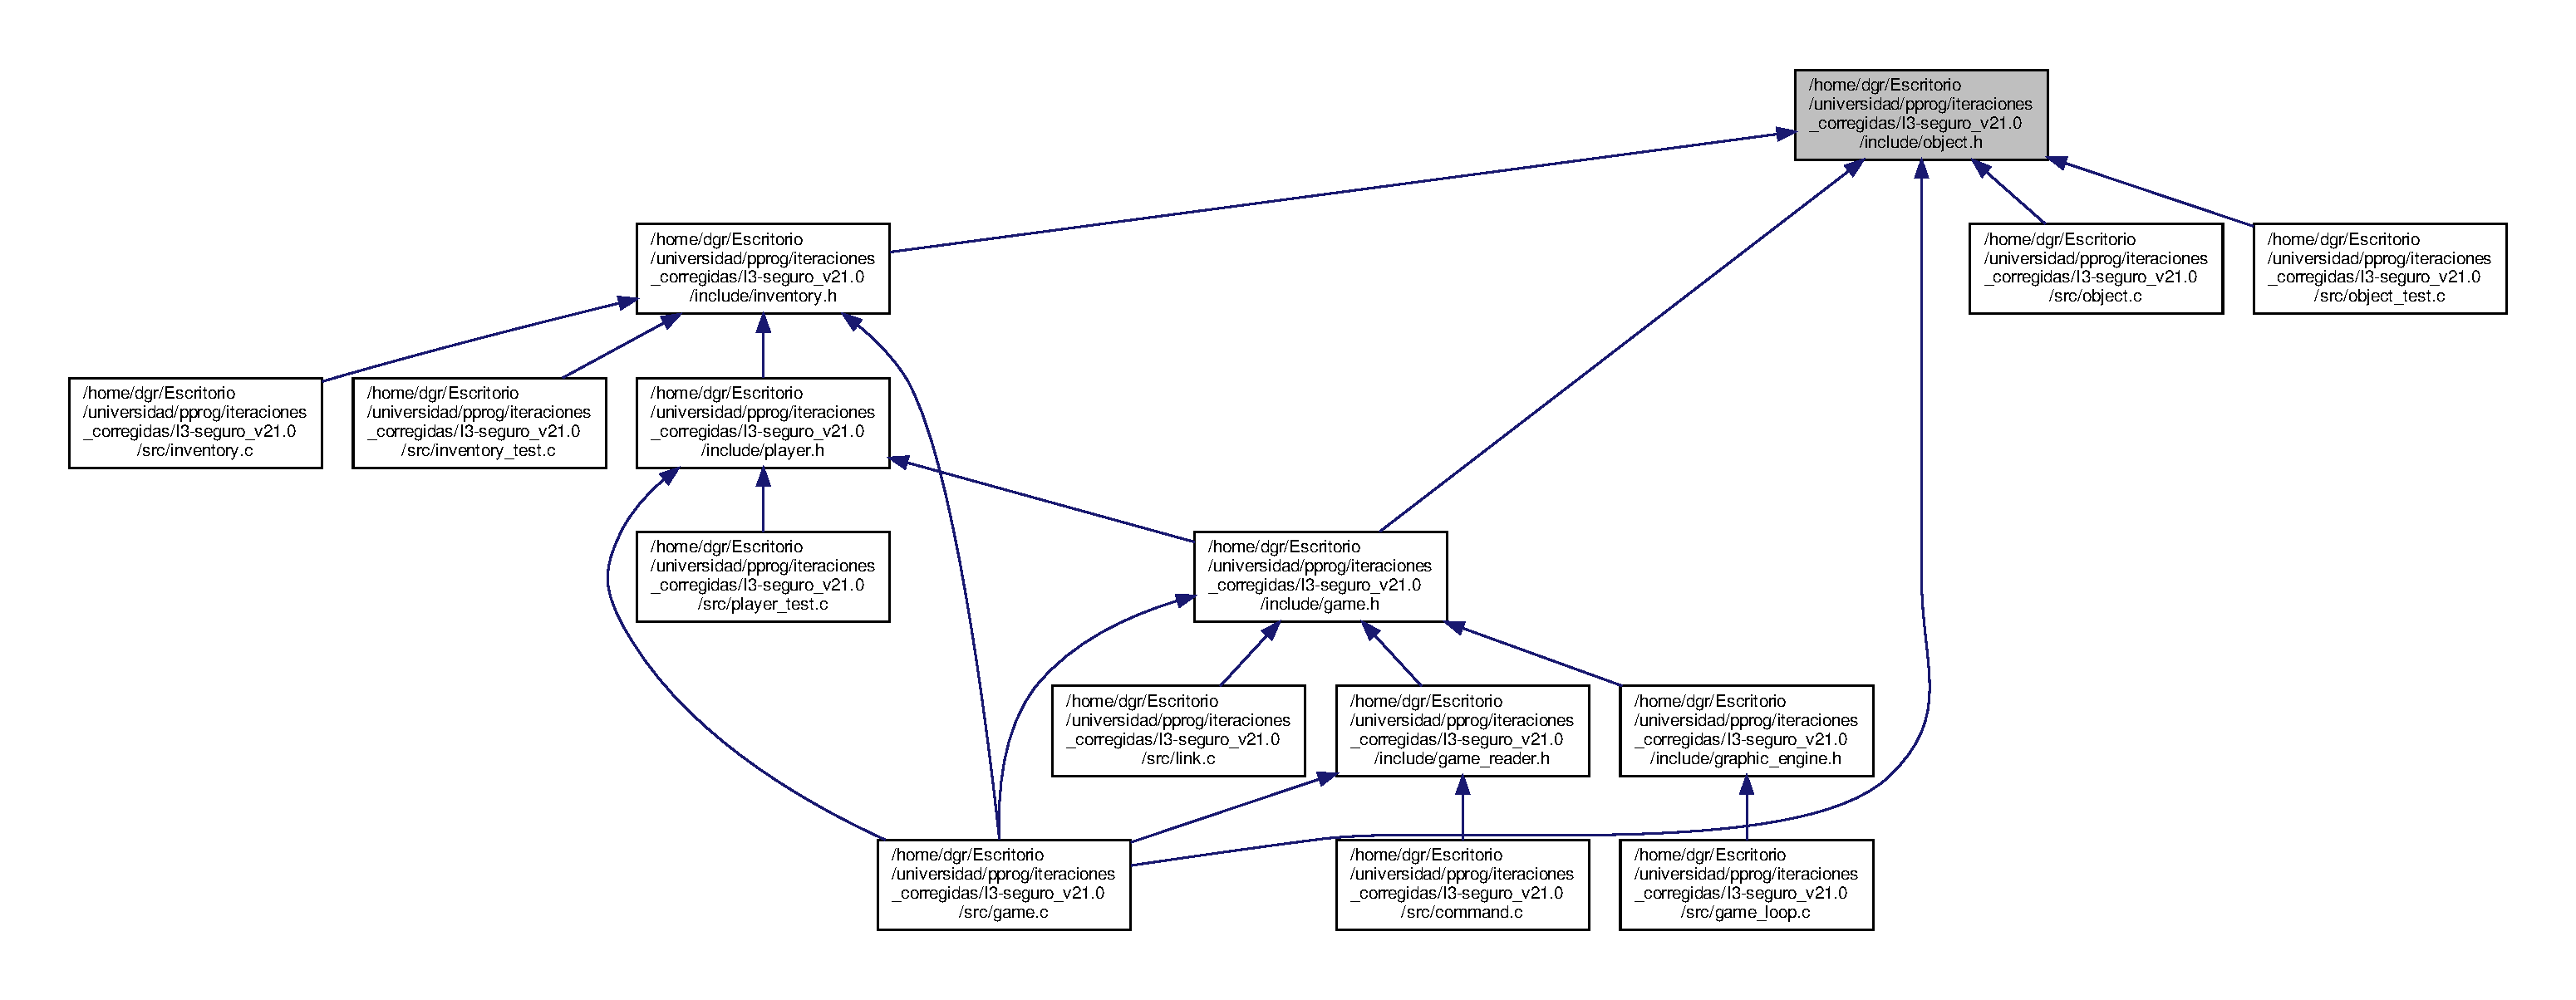
\includegraphics[width=350pt]{object_8h__dep__incl}
\end{center}
\end{figure}
\subsection*{Typedefs}
\begin{DoxyCompactItemize}
\item 
typedef struct \hyperlink{struct__Object}{\+\_\+\+Object} \hyperlink{object_8h_a7f8bbcda919b65ce67f92fba08e0212f}{Object}
\begin{DoxyCompactList}\small\item\em A type definition for a object. \end{DoxyCompactList}\end{DoxyCompactItemize}
\subsection*{Functions}
\begin{DoxyCompactItemize}
\item 
\hyperlink{object_8h_a7f8bbcda919b65ce67f92fba08e0212f}{Object} $\ast$ \hyperlink{object_8h_abb0cd30fca5fbddf137c6c04df66bbc7}{object\+\_\+create} (\hyperlink{types_8h_a845e604fb28f7e3d97549da3448149d3}{Id} id)
\begin{DoxyCompactList}\small\item\em Create the object. \end{DoxyCompactList}\item 
\hyperlink{types_8h_a32c27cc471df37f4fc818d65de0a56c4}{S\+T\+A\+T\+US} \hyperlink{object_8h_a19d6d51fee809e3801893eefc789f4b4}{object\+\_\+destroy} (\hyperlink{object_8h_a7f8bbcda919b65ce67f92fba08e0212f}{Object} $\ast$object)
\begin{DoxyCompactList}\small\item\em free an object \end{DoxyCompactList}\item 
\hyperlink{types_8h_a32c27cc471df37f4fc818d65de0a56c4}{S\+T\+A\+T\+US} \hyperlink{object_8h_ac15dc062c857503ec0ca66037caffd80}{object\+\_\+set\+\_\+name} (\hyperlink{object_8h_a7f8bbcda919b65ce67f92fba08e0212f}{Object} $\ast$object, char $\ast$name)
\begin{DoxyCompactList}\small\item\em name the object \end{DoxyCompactList}\item 
\hyperlink{types_8h_a32c27cc471df37f4fc818d65de0a56c4}{S\+T\+A\+T\+US} \hyperlink{object_8h_a6e1125f2d373ef5e9421d0a83e7a0b02}{object\+\_\+set\+\_\+id} (\hyperlink{object_8h_a7f8bbcda919b65ce67f92fba08e0212f}{Object} $\ast$object, int id)
\begin{DoxyCompactList}\small\item\em set the id \end{DoxyCompactList}\item 
const char $\ast$ \hyperlink{object_8h_a19320eebcbbd38533a18c741b804b584}{object\+\_\+get\+\_\+name} (\hyperlink{object_8h_a7f8bbcda919b65ce67f92fba08e0212f}{Object} $\ast$object)
\begin{DoxyCompactList}\small\item\em get the name of the object \end{DoxyCompactList}\item 
\hyperlink{types_8h_a845e604fb28f7e3d97549da3448149d3}{Id} \hyperlink{object_8h_ac5af152381a21853c6a28cc120e8e7fe}{object\+\_\+get\+\_\+id} (\hyperlink{object_8h_a7f8bbcda919b65ce67f92fba08e0212f}{Object} $\ast$object)
\begin{DoxyCompactList}\small\item\em get the id of the object \end{DoxyCompactList}\item 
\hyperlink{types_8h_a32c27cc471df37f4fc818d65de0a56c4}{S\+T\+A\+T\+US} \hyperlink{object_8h_adebb77fb5d33fc70616ab3b2b64c27ce}{object\+\_\+print} (\hyperlink{object_8h_a7f8bbcda919b65ce67f92fba08e0212f}{Object} $\ast$object)
\begin{DoxyCompactList}\small\item\em print the information of the object on the screen \end{DoxyCompactList}\item 
\hyperlink{types_8h_a32c27cc471df37f4fc818d65de0a56c4}{S\+T\+A\+T\+US} \hyperlink{object_8h_ae88627a8873d8f08fba9c0470a19cfc0}{object\+\_\+set\+\_\+description} (\hyperlink{object_8h_a7f8bbcda919b65ce67f92fba08e0212f}{Object} $\ast$object, char $\ast$description)
\begin{DoxyCompactList}\small\item\em set the description of an object \end{DoxyCompactList}\item 
const char $\ast$ \hyperlink{object_8h_a4b26ef1ec7057673899b58a5bf55f06a}{object\+\_\+get\+\_\+description} (\hyperlink{object_8h_a7f8bbcda919b65ce67f92fba08e0212f}{Object} $\ast$object)
\begin{DoxyCompactList}\small\item\em returns the description of an object \end{DoxyCompactList}\end{DoxyCompactItemize}


\subsection{Detailed Description}
It defines the object interface for each command. 

\begin{DoxyAuthor}{Author}
David Teófilo Garitagoitia Romero y José Manuel García Giráldez 
\end{DoxyAuthor}
\begin{DoxyVersion}{Version}
1.\+0 
\end{DoxyVersion}
\begin{DoxyDate}{Date}
9-\/02-\/2020 
\end{DoxyDate}
\begin{DoxyCopyright}{Copyright}
G\+NU Public License 
\end{DoxyCopyright}


\subsection{Typedef Documentation}
\mbox{\Hypertarget{object_8h_a7f8bbcda919b65ce67f92fba08e0212f}\label{object_8h_a7f8bbcda919b65ce67f92fba08e0212f}} 
\index{object.\+h@{object.\+h}!Object@{Object}}
\index{Object@{Object}!object.\+h@{object.\+h}}
\subsubsection{\texorpdfstring{Object}{Object}}
{\footnotesize\ttfamily typedef struct \hyperlink{struct__Object}{\+\_\+\+Object} \hyperlink{object_8h_a7f8bbcda919b65ce67f92fba08e0212f}{Object}}



A type definition for a object. 

Details. 

\subsection{Function Documentation}
\mbox{\Hypertarget{object_8h_abb0cd30fca5fbddf137c6c04df66bbc7}\label{object_8h_abb0cd30fca5fbddf137c6c04df66bbc7}} 
\index{object.\+h@{object.\+h}!object\+\_\+create@{object\+\_\+create}}
\index{object\+\_\+create@{object\+\_\+create}!object.\+h@{object.\+h}}
\subsubsection{\texorpdfstring{object\+\_\+create()}{object\_create()}}
{\footnotesize\ttfamily \hyperlink{object_8h_a7f8bbcda919b65ce67f92fba08e0212f}{Object}$\ast$ object\+\_\+create (\begin{DoxyParamCaption}\item[{\hyperlink{types_8h_a845e604fb28f7e3d97549da3448149d3}{Id}}]{id }\end{DoxyParamCaption})}



Create the object. 

object\+\_\+create Create a object with a specific Id

\begin{DoxyDate}{Date}
07-\/02-\/2019 
\end{DoxyDate}
\begin{DoxyAuthor}{Author}
\+: José Manuel García Giráldez
\end{DoxyAuthor}

\begin{DoxyParams}{Parameters}
{\em id} & the id of the new object \\
\hline
\end{DoxyParams}
\begin{DoxyReturn}{Returns}
the new object that has been created 
\end{DoxyReturn}
\mbox{\Hypertarget{object_8h_a19d6d51fee809e3801893eefc789f4b4}\label{object_8h_a19d6d51fee809e3801893eefc789f4b4}} 
\index{object.\+h@{object.\+h}!object\+\_\+destroy@{object\+\_\+destroy}}
\index{object\+\_\+destroy@{object\+\_\+destroy}!object.\+h@{object.\+h}}
\subsubsection{\texorpdfstring{object\+\_\+destroy()}{object\_destroy()}}
{\footnotesize\ttfamily \hyperlink{types_8h_a32c27cc471df37f4fc818d65de0a56c4}{S\+T\+A\+T\+US} object\+\_\+destroy (\begin{DoxyParamCaption}\item[{\hyperlink{object_8h_a7f8bbcda919b65ce67f92fba08e0212f}{Object} $\ast$}]{object }\end{DoxyParamCaption})}



free an object 

object\+\_\+destroy free a especific object

\begin{DoxyDate}{Date}
07-\/02-\/2019 
\end{DoxyDate}
\begin{DoxyAuthor}{Author}
\+: José Manuel García Giráldez
\end{DoxyAuthor}

\begin{DoxyParams}{Parameters}
{\em object} & one object that has been created before \\
\hline
\end{DoxyParams}
\begin{DoxyReturn}{Returns}
E\+R\+R\+OR if there is an error, otherwise return OK 
\end{DoxyReturn}
\mbox{\Hypertarget{object_8h_a4b26ef1ec7057673899b58a5bf55f06a}\label{object_8h_a4b26ef1ec7057673899b58a5bf55f06a}} 
\index{object.\+h@{object.\+h}!object\+\_\+get\+\_\+description@{object\+\_\+get\+\_\+description}}
\index{object\+\_\+get\+\_\+description@{object\+\_\+get\+\_\+description}!object.\+h@{object.\+h}}
\subsubsection{\texorpdfstring{object\+\_\+get\+\_\+description()}{object\_get\_description()}}
{\footnotesize\ttfamily const char$\ast$ object\+\_\+get\+\_\+description (\begin{DoxyParamCaption}\item[{\hyperlink{object_8h_a7f8bbcda919b65ce67f92fba08e0212f}{Object} $\ast$}]{object }\end{DoxyParamCaption})}



returns the description of an object 

object\+\_\+get\+\_\+description

\begin{DoxyDate}{Date}
17-\/02-\/2019 
\end{DoxyDate}
\begin{DoxyAuthor}{Author}
\+: David Teófilo Garitagoitia Romero
\end{DoxyAuthor}

\begin{DoxyParams}{Parameters}
{\em object} & one object that has been created before \\
\hline
\end{DoxyParams}
\begin{DoxyReturn}{Returns}
the description of an object 
\end{DoxyReturn}
\mbox{\Hypertarget{object_8h_ac5af152381a21853c6a28cc120e8e7fe}\label{object_8h_ac5af152381a21853c6a28cc120e8e7fe}} 
\index{object.\+h@{object.\+h}!object\+\_\+get\+\_\+id@{object\+\_\+get\+\_\+id}}
\index{object\+\_\+get\+\_\+id@{object\+\_\+get\+\_\+id}!object.\+h@{object.\+h}}
\subsubsection{\texorpdfstring{object\+\_\+get\+\_\+id()}{object\_get\_id()}}
{\footnotesize\ttfamily \hyperlink{types_8h_a845e604fb28f7e3d97549da3448149d3}{Id} object\+\_\+get\+\_\+id (\begin{DoxyParamCaption}\item[{\hyperlink{object_8h_a7f8bbcda919b65ce67f92fba08e0212f}{Object} $\ast$}]{object }\end{DoxyParamCaption})}



get the id of the object 

object\+\_\+get\+\_\+id

\begin{DoxyDate}{Date}
07-\/02-\/2019 
\end{DoxyDate}
\begin{DoxyAuthor}{Author}
\+: José Manuel García Giráldez
\end{DoxyAuthor}

\begin{DoxyParams}{Parameters}
{\em object} & one object that has been created before \\
\hline
\end{DoxyParams}
\begin{DoxyReturn}{Returns}
object-\/$>$id the id of the object we enter 
\end{DoxyReturn}
\mbox{\Hypertarget{object_8h_a19320eebcbbd38533a18c741b804b584}\label{object_8h_a19320eebcbbd38533a18c741b804b584}} 
\index{object.\+h@{object.\+h}!object\+\_\+get\+\_\+name@{object\+\_\+get\+\_\+name}}
\index{object\+\_\+get\+\_\+name@{object\+\_\+get\+\_\+name}!object.\+h@{object.\+h}}
\subsubsection{\texorpdfstring{object\+\_\+get\+\_\+name()}{object\_get\_name()}}
{\footnotesize\ttfamily const char$\ast$ object\+\_\+get\+\_\+name (\begin{DoxyParamCaption}\item[{\hyperlink{object_8h_a7f8bbcda919b65ce67f92fba08e0212f}{Object} $\ast$}]{object }\end{DoxyParamCaption})}



get the name of the object 

object\+\_\+get\+\_\+name

\begin{DoxyDate}{Date}
07-\/02-\/2019 
\end{DoxyDate}
\begin{DoxyAuthor}{Author}
\+: David Teófilo Garitagoitia Romero
\end{DoxyAuthor}

\begin{DoxyParams}{Parameters}
{\em object} & one object that has been created before \\
\hline
\end{DoxyParams}
\begin{DoxyReturn}{Returns}
object-\/$>$name the name of the object we enter 
\end{DoxyReturn}
\mbox{\Hypertarget{object_8h_adebb77fb5d33fc70616ab3b2b64c27ce}\label{object_8h_adebb77fb5d33fc70616ab3b2b64c27ce}} 
\index{object.\+h@{object.\+h}!object\+\_\+print@{object\+\_\+print}}
\index{object\+\_\+print@{object\+\_\+print}!object.\+h@{object.\+h}}
\subsubsection{\texorpdfstring{object\+\_\+print()}{object\_print()}}
{\footnotesize\ttfamily \hyperlink{types_8h_a32c27cc471df37f4fc818d65de0a56c4}{S\+T\+A\+T\+US} object\+\_\+print (\begin{DoxyParamCaption}\item[{\hyperlink{object_8h_a7f8bbcda919b65ce67f92fba08e0212f}{Object} $\ast$}]{object }\end{DoxyParamCaption})}



print the information of the object on the screen 

object\+\_\+print

\begin{DoxyDate}{Date}
07-\/02-\/2019 
\end{DoxyDate}
\begin{DoxyAuthor}{Author}
\+: David Teófilo Garitagoitia Romero
\end{DoxyAuthor}

\begin{DoxyParams}{Parameters}
{\em object} & one object that has been created before \\
\hline
\end{DoxyParams}
\begin{DoxyReturn}{Returns}
E\+R\+R\+OR if there is an error, otherwise return OK 
\end{DoxyReturn}
\mbox{\Hypertarget{object_8h_ae88627a8873d8f08fba9c0470a19cfc0}\label{object_8h_ae88627a8873d8f08fba9c0470a19cfc0}} 
\index{object.\+h@{object.\+h}!object\+\_\+set\+\_\+description@{object\+\_\+set\+\_\+description}}
\index{object\+\_\+set\+\_\+description@{object\+\_\+set\+\_\+description}!object.\+h@{object.\+h}}
\subsubsection{\texorpdfstring{object\+\_\+set\+\_\+description()}{object\_set\_description()}}
{\footnotesize\ttfamily \hyperlink{types_8h_a32c27cc471df37f4fc818d65de0a56c4}{S\+T\+A\+T\+US} object\+\_\+set\+\_\+description (\begin{DoxyParamCaption}\item[{\hyperlink{object_8h_a7f8bbcda919b65ce67f92fba08e0212f}{Object} $\ast$}]{object,  }\item[{char $\ast$}]{description }\end{DoxyParamCaption})}



set the description of an object 

object\+\_\+set\+\_\+description

\begin{DoxyDate}{Date}
17-\/02-\/2019 
\end{DoxyDate}
\begin{DoxyAuthor}{Author}
\+: David Teófilo Garitagoitia Romero
\end{DoxyAuthor}

\begin{DoxyParams}{Parameters}
{\em object} & one object that has been created before \\
\hline
{\em description} & the description we want to insert in the object \\
\hline
\end{DoxyParams}
\begin{DoxyReturn}{Returns}
E\+R\+R\+OR if there is an error, otherwise return OK 
\end{DoxyReturn}
\mbox{\Hypertarget{object_8h_a6e1125f2d373ef5e9421d0a83e7a0b02}\label{object_8h_a6e1125f2d373ef5e9421d0a83e7a0b02}} 
\index{object.\+h@{object.\+h}!object\+\_\+set\+\_\+id@{object\+\_\+set\+\_\+id}}
\index{object\+\_\+set\+\_\+id@{object\+\_\+set\+\_\+id}!object.\+h@{object.\+h}}
\subsubsection{\texorpdfstring{object\+\_\+set\+\_\+id()}{object\_set\_id()}}
{\footnotesize\ttfamily \hyperlink{types_8h_a32c27cc471df37f4fc818d65de0a56c4}{S\+T\+A\+T\+US} object\+\_\+set\+\_\+id (\begin{DoxyParamCaption}\item[{\hyperlink{object_8h_a7f8bbcda919b65ce67f92fba08e0212f}{Object} $\ast$}]{object,  }\item[{int}]{id }\end{DoxyParamCaption})}



set the id 

object\+\_\+set\+\_\+id

\begin{DoxyDate}{Date}
07-\/02-\/2019 
\end{DoxyDate}
\begin{DoxyAuthor}{Author}
\+: David Teófilo Garitagoitia Romero
\end{DoxyAuthor}

\begin{DoxyParams}{Parameters}
{\em object} & one object that has been created before \\
\hline
{\em id} & the id that the object will have \\
\hline
\end{DoxyParams}
\begin{DoxyReturn}{Returns}
E\+R\+R\+OR if there is an error, otherwise return OK 
\end{DoxyReturn}
\mbox{\Hypertarget{object_8h_ac15dc062c857503ec0ca66037caffd80}\label{object_8h_ac15dc062c857503ec0ca66037caffd80}} 
\index{object.\+h@{object.\+h}!object\+\_\+set\+\_\+name@{object\+\_\+set\+\_\+name}}
\index{object\+\_\+set\+\_\+name@{object\+\_\+set\+\_\+name}!object.\+h@{object.\+h}}
\subsubsection{\texorpdfstring{object\+\_\+set\+\_\+name()}{object\_set\_name()}}
{\footnotesize\ttfamily \hyperlink{types_8h_a32c27cc471df37f4fc818d65de0a56c4}{S\+T\+A\+T\+US} object\+\_\+set\+\_\+name (\begin{DoxyParamCaption}\item[{\hyperlink{object_8h_a7f8bbcda919b65ce67f92fba08e0212f}{Object} $\ast$}]{object,  }\item[{char $\ast$}]{name }\end{DoxyParamCaption})}



name the object 

object\+\_\+set\+\_\+name

\begin{DoxyDate}{Date}
07-\/02-\/2019 
\end{DoxyDate}
\begin{DoxyAuthor}{Author}
\+: David Teófilo Garitagoitia Romero
\end{DoxyAuthor}

\begin{DoxyParams}{Parameters}
{\em object} & one object that has been created before \\
\hline
{\em name} & the name that the object will have \\
\hline
\end{DoxyParams}
\begin{DoxyReturn}{Returns}
E\+R\+R\+OR if there is an error, otherwise return OK 
\end{DoxyReturn}

\hypertarget{object__test_8h}{}\section{/home/dgr/\+Escritorio/universidad/pprog/iteraciones\+\_\+corregidas/\+I3-\/seguro\+\_\+v21.0/include/object\+\_\+test.h File Reference}
\label{object__test_8h}\index{/home/dgr/\+Escritorio/universidad/pprog/iteraciones\+\_\+corregidas/\+I3-\/seguro\+\_\+v21.\+0/include/object\+\_\+test.\+h@{/home/dgr/\+Escritorio/universidad/pprog/iteraciones\+\_\+corregidas/\+I3-\/seguro\+\_\+v21.\+0/include/object\+\_\+test.\+h}}


It declares the tests for the object module.  


This graph shows which files directly or indirectly include this file\+:
\nopagebreak
\begin{figure}[H]
\begin{center}
\leavevmode
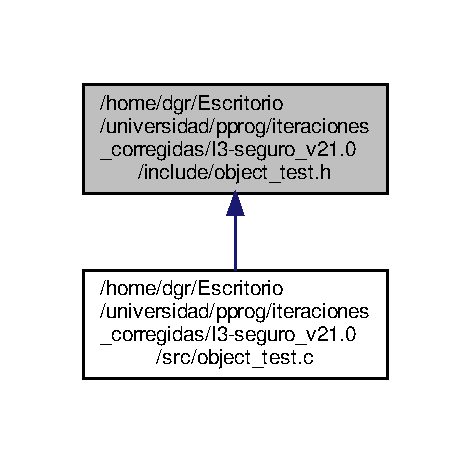
\includegraphics[width=226pt]{object__test_8h__dep__incl}
\end{center}
\end{figure}
\subsection*{Functions}
\begin{DoxyCompactItemize}
\item 
void \hyperlink{object__test_8h_a3836d69f92ce7149d56bafcaec83f516}{test1\+\_\+object\+\_\+create} ()
\item 
void \hyperlink{object__test_8h_add54ab5e33a1b0a93e9ddcf73591bd9f}{test2\+\_\+object\+\_\+create} ()
\item 
void \hyperlink{object__test_8h_a74e25ad653c4a32b9922fff8e4f916fd}{test1\+\_\+object\+\_\+set\+\_\+name} ()
\item 
void \hyperlink{object__test_8h_acf42b7e7be91ede243f2aaa56c4c9347}{test2\+\_\+object\+\_\+set\+\_\+name} ()
\item 
void \hyperlink{object__test_8h_afb26b8c66d332354df8bfd57a8033b8f}{test1\+\_\+object\+\_\+set\+\_\+description} ()
\item 
void \hyperlink{object__test_8h_a65e32c3642c1d9207cdd84b134c616da}{test2\+\_\+object\+\_\+set\+\_\+description} ()
\item 
void \hyperlink{object__test_8h_afe180b78a201df7bc1629701db1d464c}{test1\+\_\+object\+\_\+get\+\_\+description} ()
\item 
void \hyperlink{object__test_8h_a35d9a40796133791c157c044ea1cef85}{test2\+\_\+object\+\_\+get\+\_\+description} ()
\item 
void \hyperlink{object__test_8h_aa88e9e9dab92ba9c58851d7a7a8415f0}{test1\+\_\+object\+\_\+get\+\_\+id} ()
\item 
void \hyperlink{object__test_8h_a1ff250f0f43297f57fcce1f3a6ae490b}{test2\+\_\+object\+\_\+get\+\_\+id} ()
\item 
void \hyperlink{object__test_8h_ad2411bc3cc47c9905e63a3d9c561d369}{test1\+\_\+object\+\_\+get\+\_\+name} ()
\item 
void \hyperlink{object__test_8h_abdfafbc7b8588d3dcdb05fd2beb2397e}{test2\+\_\+object\+\_\+get\+\_\+name} ()
\end{DoxyCompactItemize}


\subsection{Detailed Description}
It declares the tests for the object module. 

\begin{DoxyAuthor}{Author}
Daniel Cerrato Sánchez 
\end{DoxyAuthor}
\begin{DoxyVersion}{Version}
1.\+0 
\end{DoxyVersion}
\begin{DoxyDate}{Date}
10-\/06-\/2020 
\end{DoxyDate}
\begin{DoxyCopyright}{Copyright}
G\+NU Public License 
\end{DoxyCopyright}


\subsection{Function Documentation}
\mbox{\Hypertarget{object__test_8h_a3836d69f92ce7149d56bafcaec83f516}\label{object__test_8h_a3836d69f92ce7149d56bafcaec83f516}} 
\index{object\+\_\+test.\+h@{object\+\_\+test.\+h}!test1\+\_\+object\+\_\+create@{test1\+\_\+object\+\_\+create}}
\index{test1\+\_\+object\+\_\+create@{test1\+\_\+object\+\_\+create}!object\+\_\+test.\+h@{object\+\_\+test.\+h}}
\subsubsection{\texorpdfstring{test1\+\_\+object\+\_\+create()}{test1\_object\_create()}}
{\footnotesize\ttfamily void test1\+\_\+object\+\_\+create (\begin{DoxyParamCaption}{ }\end{DoxyParamCaption})}

\begin{DoxyRefDesc}{Test}
\item[\hyperlink{test__test000103}{Test}]Test the function of creating an object \end{DoxyRefDesc}
\begin{DoxyPrecond}{Precondition}
An id as parameter 
\end{DoxyPrecond}
\begin{DoxyPostcond}{Postcondition}
A non-\/null pointer to the created object 
\end{DoxyPostcond}
\mbox{\Hypertarget{object__test_8h_afe180b78a201df7bc1629701db1d464c}\label{object__test_8h_afe180b78a201df7bc1629701db1d464c}} 
\index{object\+\_\+test.\+h@{object\+\_\+test.\+h}!test1\+\_\+object\+\_\+get\+\_\+description@{test1\+\_\+object\+\_\+get\+\_\+description}}
\index{test1\+\_\+object\+\_\+get\+\_\+description@{test1\+\_\+object\+\_\+get\+\_\+description}!object\+\_\+test.\+h@{object\+\_\+test.\+h}}
\subsubsection{\texorpdfstring{test1\+\_\+object\+\_\+get\+\_\+description()}{test1\_object\_get\_description()}}
{\footnotesize\ttfamily void test1\+\_\+object\+\_\+get\+\_\+description (\begin{DoxyParamCaption}{ }\end{DoxyParamCaption})}

\begin{DoxyRefDesc}{Test}
\item[\hyperlink{test__test000109}{Test}]Test the function to get the description of an object \end{DoxyRefDesc}
\begin{DoxyPrecond}{Precondition}
The object is a non-\/\+N\+U\+LL pointer with correct description 
\end{DoxyPrecond}
\begin{DoxyPostcond}{Postcondition}
The comparison between the description and the phrase to compare must be 0 
\end{DoxyPostcond}
\mbox{\Hypertarget{object__test_8h_aa88e9e9dab92ba9c58851d7a7a8415f0}\label{object__test_8h_aa88e9e9dab92ba9c58851d7a7a8415f0}} 
\index{object\+\_\+test.\+h@{object\+\_\+test.\+h}!test1\+\_\+object\+\_\+get\+\_\+id@{test1\+\_\+object\+\_\+get\+\_\+id}}
\index{test1\+\_\+object\+\_\+get\+\_\+id@{test1\+\_\+object\+\_\+get\+\_\+id}!object\+\_\+test.\+h@{object\+\_\+test.\+h}}
\subsubsection{\texorpdfstring{test1\+\_\+object\+\_\+get\+\_\+id()}{test1\_object\_get\_id()}}
{\footnotesize\ttfamily void test1\+\_\+object\+\_\+get\+\_\+id (\begin{DoxyParamCaption}{ }\end{DoxyParamCaption})}

\begin{DoxyRefDesc}{Test}
\item[\hyperlink{test__test000111}{Test}]Test the function to get the id of an object \end{DoxyRefDesc}
\begin{DoxyPrecond}{Precondition}
The object is a non-\/\+N\+U\+LL pointer with correct id 
\end{DoxyPrecond}
\begin{DoxyPostcond}{Postcondition}
The output must be the correct id 
\end{DoxyPostcond}
\mbox{\Hypertarget{object__test_8h_ad2411bc3cc47c9905e63a3d9c561d369}\label{object__test_8h_ad2411bc3cc47c9905e63a3d9c561d369}} 
\index{object\+\_\+test.\+h@{object\+\_\+test.\+h}!test1\+\_\+object\+\_\+get\+\_\+name@{test1\+\_\+object\+\_\+get\+\_\+name}}
\index{test1\+\_\+object\+\_\+get\+\_\+name@{test1\+\_\+object\+\_\+get\+\_\+name}!object\+\_\+test.\+h@{object\+\_\+test.\+h}}
\subsubsection{\texorpdfstring{test1\+\_\+object\+\_\+get\+\_\+name()}{test1\_object\_get\_name()}}
{\footnotesize\ttfamily void test1\+\_\+object\+\_\+get\+\_\+name (\begin{DoxyParamCaption}{ }\end{DoxyParamCaption})}

\begin{DoxyRefDesc}{Test}
\item[\hyperlink{test__test000113}{Test}]Test the function to get the name of an object \end{DoxyRefDesc}
\begin{DoxyPrecond}{Precondition}
Object is a non-\/\+N\+U\+LL pointer with correct name 
\end{DoxyPrecond}
\begin{DoxyPostcond}{Postcondition}
The comparison between the name and the word to compare must be 0 
\end{DoxyPostcond}
\mbox{\Hypertarget{object__test_8h_afb26b8c66d332354df8bfd57a8033b8f}\label{object__test_8h_afb26b8c66d332354df8bfd57a8033b8f}} 
\index{object\+\_\+test.\+h@{object\+\_\+test.\+h}!test1\+\_\+object\+\_\+set\+\_\+description@{test1\+\_\+object\+\_\+set\+\_\+description}}
\index{test1\+\_\+object\+\_\+set\+\_\+description@{test1\+\_\+object\+\_\+set\+\_\+description}!object\+\_\+test.\+h@{object\+\_\+test.\+h}}
\subsubsection{\texorpdfstring{test1\+\_\+object\+\_\+set\+\_\+description()}{test1\_object\_set\_description()}}
{\footnotesize\ttfamily void test1\+\_\+object\+\_\+set\+\_\+description (\begin{DoxyParamCaption}{ }\end{DoxyParamCaption})}

\begin{DoxyRefDesc}{Test}
\item[\hyperlink{test__test000107}{Test}]Test the function to change the description of an object \end{DoxyRefDesc}
\begin{DoxyPrecond}{Precondition}
The object is a non-\/\+N\+U\+LL pointer, the description is correct 
\end{DoxyPrecond}
\begin{DoxyPostcond}{Postcondition}
The output must be OK 
\end{DoxyPostcond}
\mbox{\Hypertarget{object__test_8h_a74e25ad653c4a32b9922fff8e4f916fd}\label{object__test_8h_a74e25ad653c4a32b9922fff8e4f916fd}} 
\index{object\+\_\+test.\+h@{object\+\_\+test.\+h}!test1\+\_\+object\+\_\+set\+\_\+name@{test1\+\_\+object\+\_\+set\+\_\+name}}
\index{test1\+\_\+object\+\_\+set\+\_\+name@{test1\+\_\+object\+\_\+set\+\_\+name}!object\+\_\+test.\+h@{object\+\_\+test.\+h}}
\subsubsection{\texorpdfstring{test1\+\_\+object\+\_\+set\+\_\+name()}{test1\_object\_set\_name()}}
{\footnotesize\ttfamily void test1\+\_\+object\+\_\+set\+\_\+name (\begin{DoxyParamCaption}{ }\end{DoxyParamCaption})}

\begin{DoxyRefDesc}{Test}
\item[\hyperlink{test__test000105}{Test}]Test the function to rename an object \end{DoxyRefDesc}
\begin{DoxyPrecond}{Precondition}
The object is a non-\/\+N\+U\+LL pointer, the name is correct 
\end{DoxyPrecond}
\begin{DoxyPostcond}{Postcondition}
The output must be OK 
\end{DoxyPostcond}
\mbox{\Hypertarget{object__test_8h_add54ab5e33a1b0a93e9ddcf73591bd9f}\label{object__test_8h_add54ab5e33a1b0a93e9ddcf73591bd9f}} 
\index{object\+\_\+test.\+h@{object\+\_\+test.\+h}!test2\+\_\+object\+\_\+create@{test2\+\_\+object\+\_\+create}}
\index{test2\+\_\+object\+\_\+create@{test2\+\_\+object\+\_\+create}!object\+\_\+test.\+h@{object\+\_\+test.\+h}}
\subsubsection{\texorpdfstring{test2\+\_\+object\+\_\+create()}{test2\_object\_create()}}
{\footnotesize\ttfamily void test2\+\_\+object\+\_\+create (\begin{DoxyParamCaption}{ }\end{DoxyParamCaption})}

\begin{DoxyRefDesc}{Test}
\item[\hyperlink{test__test000104}{Test}]Test the function of creating an object \end{DoxyRefDesc}
\begin{DoxyPrecond}{Precondition}
The object is a non-\/\+N\+U\+LL pointer with correct id 
\end{DoxyPrecond}
\begin{DoxyPostcond}{Postcondition}
The object id must be the one entered when creating it 
\end{DoxyPostcond}
\mbox{\Hypertarget{object__test_8h_a35d9a40796133791c157c044ea1cef85}\label{object__test_8h_a35d9a40796133791c157c044ea1cef85}} 
\index{object\+\_\+test.\+h@{object\+\_\+test.\+h}!test2\+\_\+object\+\_\+get\+\_\+description@{test2\+\_\+object\+\_\+get\+\_\+description}}
\index{test2\+\_\+object\+\_\+get\+\_\+description@{test2\+\_\+object\+\_\+get\+\_\+description}!object\+\_\+test.\+h@{object\+\_\+test.\+h}}
\subsubsection{\texorpdfstring{test2\+\_\+object\+\_\+get\+\_\+description()}{test2\_object\_get\_description()}}
{\footnotesize\ttfamily void test2\+\_\+object\+\_\+get\+\_\+description (\begin{DoxyParamCaption}{ }\end{DoxyParamCaption})}

\begin{DoxyRefDesc}{Test}
\item[\hyperlink{test__test000110}{Test}]Test the function to get the description of an object \end{DoxyRefDesc}
\begin{DoxyPrecond}{Precondition}
The object is a pointer to N\+U\+LL 
\end{DoxyPrecond}
\begin{DoxyPostcond}{Postcondition}
The output must be N\+U\+LL 
\end{DoxyPostcond}
\mbox{\Hypertarget{object__test_8h_a1ff250f0f43297f57fcce1f3a6ae490b}\label{object__test_8h_a1ff250f0f43297f57fcce1f3a6ae490b}} 
\index{object\+\_\+test.\+h@{object\+\_\+test.\+h}!test2\+\_\+object\+\_\+get\+\_\+id@{test2\+\_\+object\+\_\+get\+\_\+id}}
\index{test2\+\_\+object\+\_\+get\+\_\+id@{test2\+\_\+object\+\_\+get\+\_\+id}!object\+\_\+test.\+h@{object\+\_\+test.\+h}}
\subsubsection{\texorpdfstring{test2\+\_\+object\+\_\+get\+\_\+id()}{test2\_object\_get\_id()}}
{\footnotesize\ttfamily void test2\+\_\+object\+\_\+get\+\_\+id (\begin{DoxyParamCaption}{ }\end{DoxyParamCaption})}

\begin{DoxyRefDesc}{Test}
\item[\hyperlink{test__test000112}{Test}]Test the function to get the id of an object \end{DoxyRefDesc}
\begin{DoxyPrecond}{Precondition}
The object is a pointer to N\+U\+LL 
\end{DoxyPrecond}
\begin{DoxyPostcond}{Postcondition}
The output must be N\+U\+LL 
\end{DoxyPostcond}
\mbox{\Hypertarget{object__test_8h_abdfafbc7b8588d3dcdb05fd2beb2397e}\label{object__test_8h_abdfafbc7b8588d3dcdb05fd2beb2397e}} 
\index{object\+\_\+test.\+h@{object\+\_\+test.\+h}!test2\+\_\+object\+\_\+get\+\_\+name@{test2\+\_\+object\+\_\+get\+\_\+name}}
\index{test2\+\_\+object\+\_\+get\+\_\+name@{test2\+\_\+object\+\_\+get\+\_\+name}!object\+\_\+test.\+h@{object\+\_\+test.\+h}}
\subsubsection{\texorpdfstring{test2\+\_\+object\+\_\+get\+\_\+name()}{test2\_object\_get\_name()}}
{\footnotesize\ttfamily void test2\+\_\+object\+\_\+get\+\_\+name (\begin{DoxyParamCaption}{ }\end{DoxyParamCaption})}

\begin{DoxyRefDesc}{Test}
\item[\hyperlink{test__test000114}{Test}]Test the function to get the name of an object \end{DoxyRefDesc}
\begin{DoxyPrecond}{Precondition}
The object is a pointer to N\+U\+LL 
\end{DoxyPrecond}
\begin{DoxyPostcond}{Postcondition}
The output must be N\+U\+LL 
\end{DoxyPostcond}
\mbox{\Hypertarget{object__test_8h_a65e32c3642c1d9207cdd84b134c616da}\label{object__test_8h_a65e32c3642c1d9207cdd84b134c616da}} 
\index{object\+\_\+test.\+h@{object\+\_\+test.\+h}!test2\+\_\+object\+\_\+set\+\_\+description@{test2\+\_\+object\+\_\+set\+\_\+description}}
\index{test2\+\_\+object\+\_\+set\+\_\+description@{test2\+\_\+object\+\_\+set\+\_\+description}!object\+\_\+test.\+h@{object\+\_\+test.\+h}}
\subsubsection{\texorpdfstring{test2\+\_\+object\+\_\+set\+\_\+description()}{test2\_object\_set\_description()}}
{\footnotesize\ttfamily void test2\+\_\+object\+\_\+set\+\_\+description (\begin{DoxyParamCaption}{ }\end{DoxyParamCaption})}

\begin{DoxyRefDesc}{Test}
\item[\hyperlink{test__test000108}{Test}]Test the function to change the description of an object \end{DoxyRefDesc}
\begin{DoxyPrecond}{Precondition}
The object is a pointer to N\+U\+LL 
\end{DoxyPrecond}
\begin{DoxyPostcond}{Postcondition}
The output must be E\+R\+R\+OR 
\end{DoxyPostcond}
\mbox{\Hypertarget{object__test_8h_acf42b7e7be91ede243f2aaa56c4c9347}\label{object__test_8h_acf42b7e7be91ede243f2aaa56c4c9347}} 
\index{object\+\_\+test.\+h@{object\+\_\+test.\+h}!test2\+\_\+object\+\_\+set\+\_\+name@{test2\+\_\+object\+\_\+set\+\_\+name}}
\index{test2\+\_\+object\+\_\+set\+\_\+name@{test2\+\_\+object\+\_\+set\+\_\+name}!object\+\_\+test.\+h@{object\+\_\+test.\+h}}
\subsubsection{\texorpdfstring{test2\+\_\+object\+\_\+set\+\_\+name()}{test2\_object\_set\_name()}}
{\footnotesize\ttfamily void test2\+\_\+object\+\_\+set\+\_\+name (\begin{DoxyParamCaption}{ }\end{DoxyParamCaption})}

\begin{DoxyRefDesc}{Test}
\item[\hyperlink{test__test000106}{Test}]Test the function to rename an object \end{DoxyRefDesc}
\begin{DoxyPrecond}{Precondition}
The object is a pointer to N\+U\+LL 
\end{DoxyPrecond}
\begin{DoxyPostcond}{Postcondition}
The output must be E\+R\+R\+OR 
\end{DoxyPostcond}

\hypertarget{player_8h}{}\section{include/player.h File Reference}
\label{player_8h}\index{include/player.\+h@{include/player.\+h}}


It defines the player interface for each command.  


{\ttfamily \#include \char`\"{}../include/types.\+h\char`\"{}}\newline
{\ttfamily \#include \char`\"{}../include/inventory.\+h\char`\"{}}\newline
Include dependency graph for player.\+h\+:\nopagebreak
\begin{figure}[H]
\begin{center}
\leavevmode
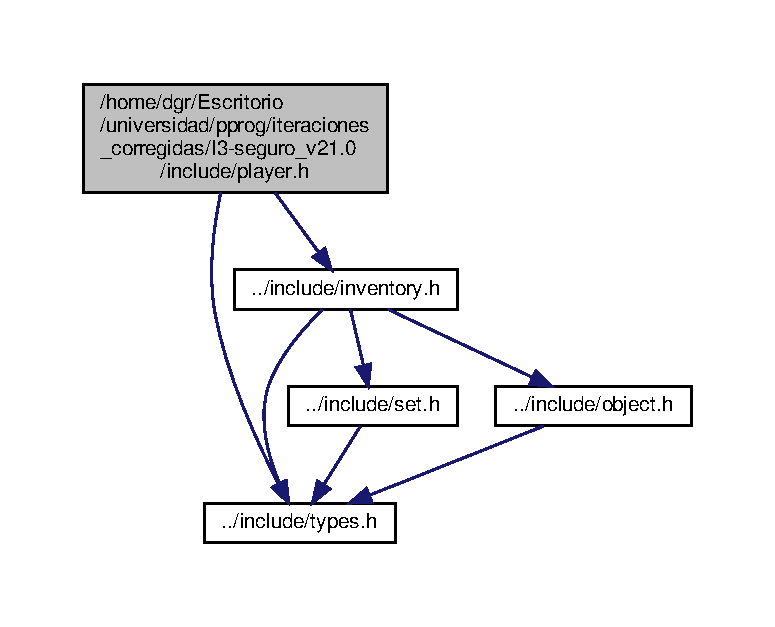
\includegraphics[width=341pt]{player_8h__incl}
\end{center}
\end{figure}
This graph shows which files directly or indirectly include this file\+:\nopagebreak
\begin{figure}[H]
\begin{center}
\leavevmode
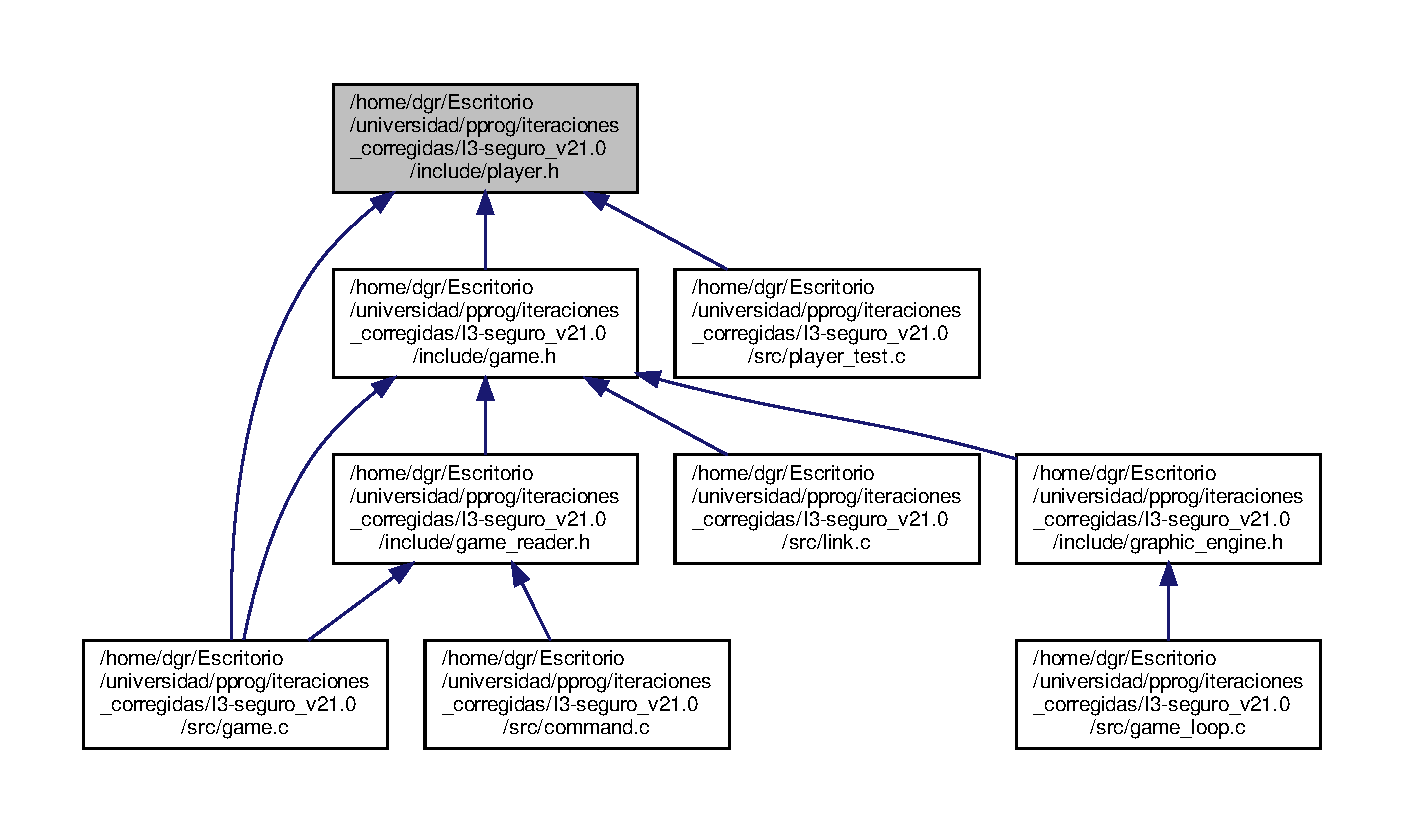
\includegraphics[width=350pt]{player_8h__dep__incl}
\end{center}
\end{figure}
\subsection*{Typedefs}
\begin{DoxyCompactItemize}
\item 
typedef struct \hyperlink{struct__Player}{\+\_\+\+Player} \hyperlink{player_8h_af30e2030635a69690f85e48bc6ef202f}{Player}
\begin{DoxyCompactList}\small\item\em A type definition for a player. \end{DoxyCompactList}\end{DoxyCompactItemize}
\subsection*{Functions}
\begin{DoxyCompactItemize}
\item 
\hyperlink{player_8h_af30e2030635a69690f85e48bc6ef202f}{Player} $\ast$ \hyperlink{player_8h_afe0bc1b421efb64a67fba4755b621209}{player\+\_\+create} (\hyperlink{types_8h_a845e604fb28f7e3d97549da3448149d3}{Id} id, int max)
\begin{DoxyCompactList}\small\item\em Create the player. \end{DoxyCompactList}\item 
\hyperlink{types_8h_a32c27cc471df37f4fc818d65de0a56c4}{S\+T\+A\+T\+US} \hyperlink{player_8h_a68e324aa5064e27d0a2f38aafb6809ad}{player\+\_\+destroy} (\hyperlink{player_8h_af30e2030635a69690f85e48bc6ef202f}{Player} $\ast$player)
\begin{DoxyCompactList}\small\item\em free a player \end{DoxyCompactList}\item 
\hyperlink{types_8h_a32c27cc471df37f4fc818d65de0a56c4}{S\+T\+A\+T\+US} \hyperlink{player_8h_a6a30809f7775f5c2d3bef47d92769e59}{player\+\_\+set\+\_\+name} (\hyperlink{player_8h_af30e2030635a69690f85e48bc6ef202f}{Player} $\ast$player, char $\ast$name)
\begin{DoxyCompactList}\small\item\em name the player \end{DoxyCompactList}\item 
\hyperlink{types_8h_a32c27cc471df37f4fc818d65de0a56c4}{S\+T\+A\+T\+US} \hyperlink{player_8h_aedae4866660857664b09dadbc6a164da}{player\+\_\+set\+\_\+id} (\hyperlink{player_8h_af30e2030635a69690f85e48bc6ef202f}{Player} $\ast$player, int id)
\begin{DoxyCompactList}\small\item\em set the id of the player \end{DoxyCompactList}\item 
\hyperlink{types_8h_a32c27cc471df37f4fc818d65de0a56c4}{S\+T\+A\+T\+US} \hyperlink{player_8h_a054e92b126f556153279b569f8987674}{player\+\_\+set\+\_\+location} (\hyperlink{player_8h_af30e2030635a69690f85e48bc6ef202f}{Player} $\ast$player, \hyperlink{types_8h_a845e604fb28f7e3d97549da3448149d3}{Id} location)
\begin{DoxyCompactList}\small\item\em set the location of the player \end{DoxyCompactList}\item 
\hyperlink{types_8h_a32c27cc471df37f4fc818d65de0a56c4}{S\+T\+A\+T\+US} \hyperlink{player_8h_a61ee43524b370147d5d9b5ccb3738048}{player\+\_\+add\+\_\+object} (\hyperlink{player_8h_af30e2030635a69690f85e48bc6ef202f}{Player} $\ast$player, \hyperlink{object_8h_a7f8bbcda919b65ce67f92fba08e0212f}{Object} $\ast$objeto)
\begin{DoxyCompactList}\small\item\em set the object that have the player \end{DoxyCompactList}\item 
const char $\ast$ \hyperlink{player_8h_a6622c02be2fe230a5c0df66385a13ece}{player\+\_\+get\+\_\+name} (\hyperlink{player_8h_af30e2030635a69690f85e48bc6ef202f}{Player} $\ast$player)
\begin{DoxyCompactList}\small\item\em get the name of the player \end{DoxyCompactList}\item 
\hyperlink{types_8h_a845e604fb28f7e3d97549da3448149d3}{Id} \hyperlink{player_8h_af5a101ec91427951c5875569a8709956}{player\+\_\+get\+\_\+id} (\hyperlink{player_8h_af30e2030635a69690f85e48bc6ef202f}{Player} $\ast$player)
\begin{DoxyCompactList}\small\item\em get the id of the player \end{DoxyCompactList}\item 
\hyperlink{types_8h_a845e604fb28f7e3d97549da3448149d3}{Id} \hyperlink{player_8h_aa50ce77ab79af7166d749619fd60acfe}{player\+\_\+get\+\_\+location} (\hyperlink{player_8h_af30e2030635a69690f85e48bc6ef202f}{Player} $\ast$player)
\begin{DoxyCompactList}\small\item\em get the location of the player \end{DoxyCompactList}\item 
\hyperlink{inventory_8h_a2253bf64ac4ce6a9c1d6f39c0b0d32a3}{Inventory} $\ast$ \hyperlink{player_8h_a270da6469a85e0c2b7f9f4088d290051}{player\+\_\+get\+\_\+inventory} (\hyperlink{player_8h_af30e2030635a69690f85e48bc6ef202f}{Player} $\ast$player)
\begin{DoxyCompactList}\small\item\em get the inventory that have the player \end{DoxyCompactList}\item 
\hyperlink{types_8h_a32c27cc471df37f4fc818d65de0a56c4}{S\+T\+A\+T\+US} \hyperlink{player_8h_aa0f2f8b4d1b63a60ef927d47aa45dbd1}{player\+\_\+print} (\hyperlink{player_8h_af30e2030635a69690f85e48bc6ef202f}{Player} $\ast$player)
\begin{DoxyCompactList}\small\item\em print the information of the player on the screen \end{DoxyCompactList}\item 
\hyperlink{types_8h_a32c27cc471df37f4fc818d65de0a56c4}{S\+T\+A\+T\+US} \hyperlink{player_8h_af3f162227798a79e835c659e9d2349e9}{player\+\_\+dell\+\_\+object} (\hyperlink{player_8h_af30e2030635a69690f85e48bc6ef202f}{Player} $\ast$player, \hyperlink{object_8h_a7f8bbcda919b65ce67f92fba08e0212f}{Object} $\ast$objeto)
\begin{DoxyCompactList}\small\item\em remove of an object that have the player \end{DoxyCompactList}\end{DoxyCompactItemize}


\subsection{Detailed Description}
It defines the player interface for each command. 

\begin{DoxyAuthor}{Author}
David Teófilo Garitagoitia Romero y José Manuel García Giráldez 
\end{DoxyAuthor}
\begin{DoxyVersion}{Version}
1.\+0 
\end{DoxyVersion}
\begin{DoxyDate}{Date}
5-\/02-\/2020 
\end{DoxyDate}
\begin{DoxyCopyright}{Copyright}
G\+NU Public License 
\end{DoxyCopyright}


\subsection{Typedef Documentation}
\mbox{\Hypertarget{player_8h_af30e2030635a69690f85e48bc6ef202f}\label{player_8h_af30e2030635a69690f85e48bc6ef202f}} 
\index{player.\+h@{player.\+h}!Player@{Player}}
\index{Player@{Player}!player.\+h@{player.\+h}}
\subsubsection{\texorpdfstring{Player}{Player}}
{\footnotesize\ttfamily typedef struct \hyperlink{struct__Player}{\+\_\+\+Player} \hyperlink{player_8h_af30e2030635a69690f85e48bc6ef202f}{Player}}



A type definition for a player. 

Details. 

\subsection{Function Documentation}
\mbox{\Hypertarget{player_8h_a61ee43524b370147d5d9b5ccb3738048}\label{player_8h_a61ee43524b370147d5d9b5ccb3738048}} 
\index{player.\+h@{player.\+h}!player\+\_\+add\+\_\+object@{player\+\_\+add\+\_\+object}}
\index{player\+\_\+add\+\_\+object@{player\+\_\+add\+\_\+object}!player.\+h@{player.\+h}}
\subsubsection{\texorpdfstring{player\+\_\+add\+\_\+object()}{player\_add\_object()}}
{\footnotesize\ttfamily \hyperlink{types_8h_a32c27cc471df37f4fc818d65de0a56c4}{S\+T\+A\+T\+US} player\+\_\+add\+\_\+object (\begin{DoxyParamCaption}\item[{\hyperlink{player_8h_af30e2030635a69690f85e48bc6ef202f}{Player} $\ast$}]{player,  }\item[{\hyperlink{object_8h_a7f8bbcda919b65ce67f92fba08e0212f}{Object} $\ast$}]{objeto }\end{DoxyParamCaption})}



set the object that have the player 

player\+\_\+add\+\_\+object

\begin{DoxyDate}{Date}
07-\/02-\/2019 
\end{DoxyDate}
\begin{DoxyAuthor}{Author}
\+: David Teófilo Garitagoitia Romero
\end{DoxyAuthor}

\begin{DoxyParams}{Parameters}
{\em player} & a player that has been created before \\
\hline
{\em objeto} & a object that will be having by the player \\
\hline
\end{DoxyParams}
\begin{DoxyReturn}{Returns}
E\+R\+R\+OR if there is an error, otherwise return OK 
\end{DoxyReturn}
\mbox{\Hypertarget{player_8h_afe0bc1b421efb64a67fba4755b621209}\label{player_8h_afe0bc1b421efb64a67fba4755b621209}} 
\index{player.\+h@{player.\+h}!player\+\_\+create@{player\+\_\+create}}
\index{player\+\_\+create@{player\+\_\+create}!player.\+h@{player.\+h}}
\subsubsection{\texorpdfstring{player\+\_\+create()}{player\_create()}}
{\footnotesize\ttfamily \hyperlink{player_8h_af30e2030635a69690f85e48bc6ef202f}{Player}$\ast$ player\+\_\+create (\begin{DoxyParamCaption}\item[{\hyperlink{types_8h_a845e604fb28f7e3d97549da3448149d3}{Id}}]{id,  }\item[{int}]{max }\end{DoxyParamCaption})}



Create the player. 

player\+\_\+create Create a player with a specific Id

\begin{DoxyDate}{Date}
07-\/02-\/2019 
\end{DoxyDate}
\begin{DoxyAuthor}{Author}
\+: José Manuel García Giráldez
\end{DoxyAuthor}

\begin{DoxyParams}{Parameters}
{\em id} & the id of the new player \\
\hline
{\em max} & the maximum number of objects that he can store \\
\hline
\end{DoxyParams}
\begin{DoxyReturn}{Returns}
the new player that has been created 
\end{DoxyReturn}
\mbox{\Hypertarget{player_8h_af3f162227798a79e835c659e9d2349e9}\label{player_8h_af3f162227798a79e835c659e9d2349e9}} 
\index{player.\+h@{player.\+h}!player\+\_\+dell\+\_\+object@{player\+\_\+dell\+\_\+object}}
\index{player\+\_\+dell\+\_\+object@{player\+\_\+dell\+\_\+object}!player.\+h@{player.\+h}}
\subsubsection{\texorpdfstring{player\+\_\+dell\+\_\+object()}{player\_dell\_object()}}
{\footnotesize\ttfamily \hyperlink{types_8h_a32c27cc471df37f4fc818d65de0a56c4}{S\+T\+A\+T\+US} player\+\_\+dell\+\_\+object (\begin{DoxyParamCaption}\item[{\hyperlink{player_8h_af30e2030635a69690f85e48bc6ef202f}{Player} $\ast$}]{player,  }\item[{\hyperlink{object_8h_a7f8bbcda919b65ce67f92fba08e0212f}{Object} $\ast$}]{objeto }\end{DoxyParamCaption})}



remove of an object that have the player 

player\+\_\+dell\+\_\+object

\begin{DoxyDate}{Date}
10-\/3-\/2020 
\end{DoxyDate}
\begin{DoxyAuthor}{Author}
\+: David Teófilo Garitagoitia Romero
\end{DoxyAuthor}

\begin{DoxyParams}{Parameters}
{\em player} & the player that have the object \\
\hline
{\em objeto} & the object that we want to delete from player \\
\hline
\end{DoxyParams}
\begin{DoxyReturn}{Returns}
E\+R\+R\+OR if there is an error, otherwise return OK 
\end{DoxyReturn}
\mbox{\Hypertarget{player_8h_a68e324aa5064e27d0a2f38aafb6809ad}\label{player_8h_a68e324aa5064e27d0a2f38aafb6809ad}} 
\index{player.\+h@{player.\+h}!player\+\_\+destroy@{player\+\_\+destroy}}
\index{player\+\_\+destroy@{player\+\_\+destroy}!player.\+h@{player.\+h}}
\subsubsection{\texorpdfstring{player\+\_\+destroy()}{player\_destroy()}}
{\footnotesize\ttfamily \hyperlink{types_8h_a32c27cc471df37f4fc818d65de0a56c4}{S\+T\+A\+T\+US} player\+\_\+destroy (\begin{DoxyParamCaption}\item[{\hyperlink{player_8h_af30e2030635a69690f85e48bc6ef202f}{Player} $\ast$}]{player }\end{DoxyParamCaption})}



free a player 

player\+\_\+destroy free a especific player

\begin{DoxyDate}{Date}
07-\/02-\/2019 
\end{DoxyDate}
\begin{DoxyAuthor}{Author}
\+: José Manuel García Giráldez
\end{DoxyAuthor}

\begin{DoxyParams}{Parameters}
{\em player} & a player that has been created before \\
\hline
\end{DoxyParams}
\begin{DoxyReturn}{Returns}
E\+R\+R\+OR if there is an error, otherwise return OK 
\end{DoxyReturn}
\mbox{\Hypertarget{player_8h_af5a101ec91427951c5875569a8709956}\label{player_8h_af5a101ec91427951c5875569a8709956}} 
\index{player.\+h@{player.\+h}!player\+\_\+get\+\_\+id@{player\+\_\+get\+\_\+id}}
\index{player\+\_\+get\+\_\+id@{player\+\_\+get\+\_\+id}!player.\+h@{player.\+h}}
\subsubsection{\texorpdfstring{player\+\_\+get\+\_\+id()}{player\_get\_id()}}
{\footnotesize\ttfamily \hyperlink{types_8h_a845e604fb28f7e3d97549da3448149d3}{Id} player\+\_\+get\+\_\+id (\begin{DoxyParamCaption}\item[{\hyperlink{player_8h_af30e2030635a69690f85e48bc6ef202f}{Player} $\ast$}]{player }\end{DoxyParamCaption})}



get the id of the player 

player\+\_\+get\+\_\+id

\begin{DoxyDate}{Date}
07-\/02-\/2019 
\end{DoxyDate}
\begin{DoxyAuthor}{Author}
\+: David Teófilo Garitagoitia Romero
\end{DoxyAuthor}

\begin{DoxyParams}{Parameters}
{\em player} & the player you want to get their id \\
\hline
\end{DoxyParams}
\begin{DoxyReturn}{Returns}
player-\/$>$id the id of the player we enter 
\end{DoxyReturn}
\mbox{\Hypertarget{player_8h_a270da6469a85e0c2b7f9f4088d290051}\label{player_8h_a270da6469a85e0c2b7f9f4088d290051}} 
\index{player.\+h@{player.\+h}!player\+\_\+get\+\_\+inventory@{player\+\_\+get\+\_\+inventory}}
\index{player\+\_\+get\+\_\+inventory@{player\+\_\+get\+\_\+inventory}!player.\+h@{player.\+h}}
\subsubsection{\texorpdfstring{player\+\_\+get\+\_\+inventory()}{player\_get\_inventory()}}
{\footnotesize\ttfamily \hyperlink{inventory_8h_a2253bf64ac4ce6a9c1d6f39c0b0d32a3}{Inventory}$\ast$ player\+\_\+get\+\_\+inventory (\begin{DoxyParamCaption}\item[{\hyperlink{player_8h_af30e2030635a69690f85e48bc6ef202f}{Player} $\ast$}]{player }\end{DoxyParamCaption})}



get the inventory that have the player 

player\+\_\+get\+\_\+inventory

\begin{DoxyDate}{Date}
14-\/02-\/2020 
\end{DoxyDate}
\begin{DoxyAuthor}{Author}
\+: David Teófilo Garitagoitia Romero
\end{DoxyAuthor}

\begin{DoxyParams}{Parameters}
{\em player} & one player that has been created before \\
\hline
\end{DoxyParams}
\begin{DoxyReturn}{Returns}
the inventory of the player we enter 
\end{DoxyReturn}
\mbox{\Hypertarget{player_8h_aa50ce77ab79af7166d749619fd60acfe}\label{player_8h_aa50ce77ab79af7166d749619fd60acfe}} 
\index{player.\+h@{player.\+h}!player\+\_\+get\+\_\+location@{player\+\_\+get\+\_\+location}}
\index{player\+\_\+get\+\_\+location@{player\+\_\+get\+\_\+location}!player.\+h@{player.\+h}}
\subsubsection{\texorpdfstring{player\+\_\+get\+\_\+location()}{player\_get\_location()}}
{\footnotesize\ttfamily \hyperlink{types_8h_a845e604fb28f7e3d97549da3448149d3}{Id} player\+\_\+get\+\_\+location (\begin{DoxyParamCaption}\item[{\hyperlink{player_8h_af30e2030635a69690f85e48bc6ef202f}{Player} $\ast$}]{player }\end{DoxyParamCaption})}



get the location of the player 

player\+\_\+get\+\_\+location

\begin{DoxyDate}{Date}
07-\/02-\/2019 
\end{DoxyDate}
\begin{DoxyAuthor}{Author}
\+: José Manuel García Giráldez
\end{DoxyAuthor}

\begin{DoxyParams}{Parameters}
{\em player} & a player that has been created before \\
\hline
\end{DoxyParams}
\begin{DoxyReturn}{Returns}
player-\/$>$location the location of the object we enter 
\end{DoxyReturn}
\mbox{\Hypertarget{player_8h_a6622c02be2fe230a5c0df66385a13ece}\label{player_8h_a6622c02be2fe230a5c0df66385a13ece}} 
\index{player.\+h@{player.\+h}!player\+\_\+get\+\_\+name@{player\+\_\+get\+\_\+name}}
\index{player\+\_\+get\+\_\+name@{player\+\_\+get\+\_\+name}!player.\+h@{player.\+h}}
\subsubsection{\texorpdfstring{player\+\_\+get\+\_\+name()}{player\_get\_name()}}
{\footnotesize\ttfamily const char$\ast$ player\+\_\+get\+\_\+name (\begin{DoxyParamCaption}\item[{\hyperlink{player_8h_af30e2030635a69690f85e48bc6ef202f}{Player} $\ast$}]{player }\end{DoxyParamCaption})}



get the name of the player 

player\+\_\+get\+\_\+name

\begin{DoxyDate}{Date}
07-\/02-\/2019 
\end{DoxyDate}
\begin{DoxyAuthor}{Author}
\+: José Manuel García Giráldez
\end{DoxyAuthor}

\begin{DoxyParams}{Parameters}
{\em player} & a player that has been created before \\
\hline
\end{DoxyParams}
\begin{DoxyReturn}{Returns}
player-\/$>$name the name of the object we enter 
\end{DoxyReturn}
\mbox{\Hypertarget{player_8h_aa0f2f8b4d1b63a60ef927d47aa45dbd1}\label{player_8h_aa0f2f8b4d1b63a60ef927d47aa45dbd1}} 
\index{player.\+h@{player.\+h}!player\+\_\+print@{player\+\_\+print}}
\index{player\+\_\+print@{player\+\_\+print}!player.\+h@{player.\+h}}
\subsubsection{\texorpdfstring{player\+\_\+print()}{player\_print()}}
{\footnotesize\ttfamily \hyperlink{types_8h_a32c27cc471df37f4fc818d65de0a56c4}{S\+T\+A\+T\+US} player\+\_\+print (\begin{DoxyParamCaption}\item[{\hyperlink{player_8h_af30e2030635a69690f85e48bc6ef202f}{Player} $\ast$}]{player }\end{DoxyParamCaption})}



print the information of the player on the screen 

player\+\_\+print

\begin{DoxyDate}{Date}
07-\/02-\/2020 
\end{DoxyDate}
\begin{DoxyAuthor}{Author}
\+: David Teófilo Garitagoitia Romero
\end{DoxyAuthor}

\begin{DoxyParams}{Parameters}
{\em player} & the player whose info you wnat to print \\
\hline
\end{DoxyParams}
\begin{DoxyReturn}{Returns}
E\+R\+R\+OR if there is an error, otherwise return OK 
\end{DoxyReturn}
\mbox{\Hypertarget{player_8h_aedae4866660857664b09dadbc6a164da}\label{player_8h_aedae4866660857664b09dadbc6a164da}} 
\index{player.\+h@{player.\+h}!player\+\_\+set\+\_\+id@{player\+\_\+set\+\_\+id}}
\index{player\+\_\+set\+\_\+id@{player\+\_\+set\+\_\+id}!player.\+h@{player.\+h}}
\subsubsection{\texorpdfstring{player\+\_\+set\+\_\+id()}{player\_set\_id()}}
{\footnotesize\ttfamily \hyperlink{types_8h_a32c27cc471df37f4fc818d65de0a56c4}{S\+T\+A\+T\+US} player\+\_\+set\+\_\+id (\begin{DoxyParamCaption}\item[{\hyperlink{player_8h_af30e2030635a69690f85e48bc6ef202f}{Player} $\ast$}]{player,  }\item[{int}]{id }\end{DoxyParamCaption})}



set the id of the player 

player\+\_\+set\+\_\+id

\begin{DoxyDate}{Date}
07-\/02-\/2019 
\end{DoxyDate}
\begin{DoxyAuthor}{Author}
\+: José Manuel García Giráldez
\end{DoxyAuthor}

\begin{DoxyParams}{Parameters}
{\em player} & the player you want to set id \\
\hline
{\em id} & the id that the object will have \\
\hline
\end{DoxyParams}
\begin{DoxyReturn}{Returns}
E\+R\+R\+OR if there is an error, otherwise return OK 
\end{DoxyReturn}
\mbox{\Hypertarget{player_8h_a054e92b126f556153279b569f8987674}\label{player_8h_a054e92b126f556153279b569f8987674}} 
\index{player.\+h@{player.\+h}!player\+\_\+set\+\_\+location@{player\+\_\+set\+\_\+location}}
\index{player\+\_\+set\+\_\+location@{player\+\_\+set\+\_\+location}!player.\+h@{player.\+h}}
\subsubsection{\texorpdfstring{player\+\_\+set\+\_\+location()}{player\_set\_location()}}
{\footnotesize\ttfamily \hyperlink{types_8h_a32c27cc471df37f4fc818d65de0a56c4}{S\+T\+A\+T\+US} player\+\_\+set\+\_\+location (\begin{DoxyParamCaption}\item[{\hyperlink{player_8h_af30e2030635a69690f85e48bc6ef202f}{Player} $\ast$}]{player,  }\item[{\hyperlink{types_8h_a845e604fb28f7e3d97549da3448149d3}{Id}}]{location }\end{DoxyParamCaption})}



set the location of the player 

player\+\_\+set\+\_\+location

\begin{DoxyDate}{Date}
07-\/02-\/2019 
\end{DoxyDate}
\begin{DoxyAuthor}{Author}
\+: David Teófilo Garitagoitia Romero
\end{DoxyAuthor}

\begin{DoxyParams}{Parameters}
{\em player} & a player that has been created before \\
\hline
{\em location} & the location that the player will have \\
\hline
\end{DoxyParams}
\begin{DoxyReturn}{Returns}
E\+R\+R\+OR if there is an error, otherwise return OK 
\end{DoxyReturn}
\mbox{\Hypertarget{player_8h_a6a30809f7775f5c2d3bef47d92769e59}\label{player_8h_a6a30809f7775f5c2d3bef47d92769e59}} 
\index{player.\+h@{player.\+h}!player\+\_\+set\+\_\+name@{player\+\_\+set\+\_\+name}}
\index{player\+\_\+set\+\_\+name@{player\+\_\+set\+\_\+name}!player.\+h@{player.\+h}}
\subsubsection{\texorpdfstring{player\+\_\+set\+\_\+name()}{player\_set\_name()}}
{\footnotesize\ttfamily \hyperlink{types_8h_a32c27cc471df37f4fc818d65de0a56c4}{S\+T\+A\+T\+US} player\+\_\+set\+\_\+name (\begin{DoxyParamCaption}\item[{\hyperlink{player_8h_af30e2030635a69690f85e48bc6ef202f}{Player} $\ast$}]{player,  }\item[{char $\ast$}]{name }\end{DoxyParamCaption})}



name the player 

player\+\_\+set-\/name

\begin{DoxyDate}{Date}
07-\/02-\/2019 
\end{DoxyDate}
\begin{DoxyAuthor}{Author}
\+: David Teófilo Garitagoitia Romero
\end{DoxyAuthor}

\begin{DoxyParams}{Parameters}
{\em player} & a player that has been created before \\
\hline
{\em name} & the name that the player will have \\
\hline
\end{DoxyParams}
\begin{DoxyReturn}{Returns}
E\+R\+R\+OR if there is an error, otherwise return OK 
\end{DoxyReturn}

\hypertarget{player__test_8h}{}\section{include/player\+\_\+test.h File Reference}
\label{player__test_8h}\index{include/player\+\_\+test.\+h@{include/player\+\_\+test.\+h}}


It declares the tests for the player module.  


This graph shows which files directly or indirectly include this file\+:\nopagebreak
\begin{figure}[H]
\begin{center}
\leavevmode
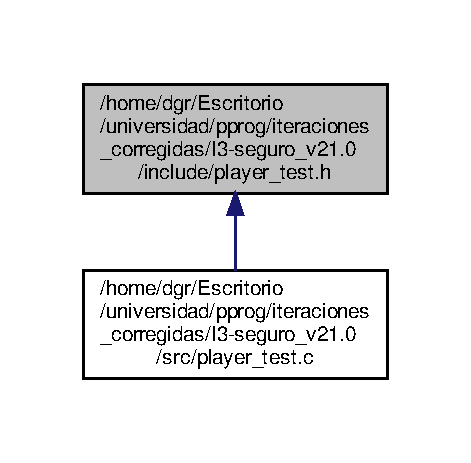
\includegraphics[width=187pt]{player__test_8h__dep__incl}
\end{center}
\end{figure}
\subsection*{Functions}
\begin{DoxyCompactItemize}
\item 
void \hyperlink{player__test_8h_ab29768452373e16bb6aaa1f7998f62fb}{test1\+\_\+player\+\_\+create} ()
\item 
void \hyperlink{player__test_8h_a4f6eca5f9d8c08d2a7fc70c209ecf854}{test2\+\_\+player\+\_\+create} ()
\item 
void \hyperlink{player__test_8h_a14a3e4867e2ad3287c8efa99cd36904e}{test1\+\_\+player\+\_\+add\+\_\+object} ()
\item 
void \hyperlink{player__test_8h_a864d3935cf61953950b10df0e656306d}{test2\+\_\+player\+\_\+add\+\_\+object} ()
\item 
void \hyperlink{player__test_8h_ac984e5292c95002644a7af4fa499d0fb}{test3\+\_\+player\+\_\+add\+\_\+object} ()
\item 
void \hyperlink{player__test_8h_a5e2baa63ffa19a8676477e060ea784ca}{test1\+\_\+player\+\_\+dell\+\_\+object} ()
\item 
void \hyperlink{player__test_8h_a4a1855514d6fbd8387f730de40437cf4}{test2\+\_\+player\+\_\+dell\+\_\+object} ()
\item 
void \hyperlink{player__test_8h_aed6b8d0d4b733a8182faef777d6bb4d7}{test3\+\_\+player\+\_\+dell\+\_\+object} ()
\item 
void \hyperlink{player__test_8h_a27b5f30b6faa1d0bf8eb97fa9083a8e2}{test4\+\_\+player\+\_\+dell\+\_\+object} ()
\item 
void \hyperlink{player__test_8h_a9d87c09e6af910d695265e3fd77ae3a2}{test1\+\_\+player\+\_\+set\+\_\+name} ()
\item 
void \hyperlink{player__test_8h_a6e7ce8ff791f4bf63749df647a44263f}{test2\+\_\+player\+\_\+set\+\_\+name} ()
\item 
void \hyperlink{player__test_8h_a94068667d8faa66a4ad293dd2c60f2ef}{test1\+\_\+player\+\_\+get\+\_\+name} ()
\item 
void \hyperlink{player__test_8h_a3aa908fd360b74e7786422260e8e16a0}{test2\+\_\+player\+\_\+get\+\_\+name} ()
\item 
void \hyperlink{player__test_8h_aec6799a4f46c3f3c471fcb668addcad4}{test1\+\_\+player\+\_\+set\+\_\+location} ()
\item 
void \hyperlink{player__test_8h_a2c702753d9e2e3df9ef4abf2d1b9bc8d}{test2\+\_\+player\+\_\+set\+\_\+location} ()
\item 
void \hyperlink{player__test_8h_a408a557a0cff748c10fb9a03445af191}{test1\+\_\+player\+\_\+get\+\_\+location} ()
\item 
void \hyperlink{player__test_8h_a4c5605fac4bd716e1dfb2744db4fa8a1}{test2\+\_\+player\+\_\+get\+\_\+location} ()
\item 
void \hyperlink{player__test_8h_a64fa15a235953bea694236b9d7841cbc}{test1\+\_\+player\+\_\+set\+\_\+id} ()
\item 
void \hyperlink{player__test_8h_a3695e0896bc3d770290e6a691fa212f7}{test2\+\_\+player\+\_\+set\+\_\+id} ()
\item 
void \hyperlink{player__test_8h_a790a75dc179c00c60c784d3e34c0e5aa}{test1\+\_\+player\+\_\+get\+\_\+id} ()
\item 
void \hyperlink{player__test_8h_a9fa80f0c0e46b45eb9f1685b102a5826}{test2\+\_\+player\+\_\+get\+\_\+id} ()
\item 
void \hyperlink{player__test_8h_ad4a86b57bc18593265c205d7b27b9ecb}{test1\+\_\+player\+\_\+get\+\_\+inventory} ()
\item 
void \hyperlink{player__test_8h_a8f3a62c708fbed848568841ca8b1cd26}{test2\+\_\+player\+\_\+get\+\_\+inventory} ()
\end{DoxyCompactItemize}


\subsection{Detailed Description}
It declares the tests for the player module. 

\begin{DoxyAuthor}{Author}
Daniel Cerrato Sánchez 
\end{DoxyAuthor}
\begin{DoxyVersion}{Version}
1.\+0 
\end{DoxyVersion}
\begin{DoxyDate}{Date}
08-\/06-\/2020 
\end{DoxyDate}
\begin{DoxyCopyright}{Copyright}
G\+NU Public License 
\end{DoxyCopyright}


\subsection{Function Documentation}
\mbox{\Hypertarget{player__test_8h_a14a3e4867e2ad3287c8efa99cd36904e}\label{player__test_8h_a14a3e4867e2ad3287c8efa99cd36904e}} 
\index{player\+\_\+test.\+h@{player\+\_\+test.\+h}!test1\+\_\+player\+\_\+add\+\_\+object@{test1\+\_\+player\+\_\+add\+\_\+object}}
\index{test1\+\_\+player\+\_\+add\+\_\+object@{test1\+\_\+player\+\_\+add\+\_\+object}!player\+\_\+test.\+h@{player\+\_\+test.\+h}}
\subsubsection{\texorpdfstring{test1\+\_\+player\+\_\+add\+\_\+object()}{test1\_player\_add\_object()}}
{\footnotesize\ttfamily void test1\+\_\+player\+\_\+add\+\_\+object (\begin{DoxyParamCaption}{ }\end{DoxyParamCaption})}

\begin{DoxyRefDesc}{Test}
\item[\hyperlink{test__test000201}{Test}]Test the function of adding an object to the player \end{DoxyRefDesc}
\begin{DoxyPrecond}{Precondition}
The player is a non-\/\+N\+U\+LL pointer, but the object is a N\+U\+LL pointer 
\end{DoxyPrecond}
\begin{DoxyPostcond}{Postcondition}
The output must be E\+R\+R\+OR 
\end{DoxyPostcond}
\mbox{\Hypertarget{player__test_8h_ab29768452373e16bb6aaa1f7998f62fb}\label{player__test_8h_ab29768452373e16bb6aaa1f7998f62fb}} 
\index{player\+\_\+test.\+h@{player\+\_\+test.\+h}!test1\+\_\+player\+\_\+create@{test1\+\_\+player\+\_\+create}}
\index{test1\+\_\+player\+\_\+create@{test1\+\_\+player\+\_\+create}!player\+\_\+test.\+h@{player\+\_\+test.\+h}}
\subsubsection{\texorpdfstring{test1\+\_\+player\+\_\+create()}{test1\_player\_create()}}
{\footnotesize\ttfamily void test1\+\_\+player\+\_\+create (\begin{DoxyParamCaption}{ }\end{DoxyParamCaption})}

\begin{DoxyRefDesc}{Test}
\item[\hyperlink{test__test000199}{Test}]Test the player creation function \end{DoxyRefDesc}
\begin{DoxyPrecond}{Precondition}
An id and an integer for the number of objects they can carry as parameters 
\end{DoxyPrecond}
\begin{DoxyPostcond}{Postcondition}
A non-\/null pointer to the created player 
\end{DoxyPostcond}
\mbox{\Hypertarget{player__test_8h_a5e2baa63ffa19a8676477e060ea784ca}\label{player__test_8h_a5e2baa63ffa19a8676477e060ea784ca}} 
\index{player\+\_\+test.\+h@{player\+\_\+test.\+h}!test1\+\_\+player\+\_\+dell\+\_\+object@{test1\+\_\+player\+\_\+dell\+\_\+object}}
\index{test1\+\_\+player\+\_\+dell\+\_\+object@{test1\+\_\+player\+\_\+dell\+\_\+object}!player\+\_\+test.\+h@{player\+\_\+test.\+h}}
\subsubsection{\texorpdfstring{test1\+\_\+player\+\_\+dell\+\_\+object()}{test1\_player\_dell\_object()}}
{\footnotesize\ttfamily void test1\+\_\+player\+\_\+dell\+\_\+object (\begin{DoxyParamCaption}{ }\end{DoxyParamCaption})}

\begin{DoxyRefDesc}{Test}
\item[\hyperlink{test__test000204}{Test}]Test the deletion function of a player object \end{DoxyRefDesc}
\begin{DoxyPrecond}{Precondition}
Player and object are non-\/\+N\+U\+LL pointers, correct object is searched 
\end{DoxyPrecond}
\begin{DoxyPostcond}{Postcondition}
The output must be OK 
\end{DoxyPostcond}
\mbox{\Hypertarget{player__test_8h_a790a75dc179c00c60c784d3e34c0e5aa}\label{player__test_8h_a790a75dc179c00c60c784d3e34c0e5aa}} 
\index{player\+\_\+test.\+h@{player\+\_\+test.\+h}!test1\+\_\+player\+\_\+get\+\_\+id@{test1\+\_\+player\+\_\+get\+\_\+id}}
\index{test1\+\_\+player\+\_\+get\+\_\+id@{test1\+\_\+player\+\_\+get\+\_\+id}!player\+\_\+test.\+h@{player\+\_\+test.\+h}}
\subsubsection{\texorpdfstring{test1\+\_\+player\+\_\+get\+\_\+id()}{test1\_player\_get\_id()}}
{\footnotesize\ttfamily void test1\+\_\+player\+\_\+get\+\_\+id (\begin{DoxyParamCaption}{ }\end{DoxyParamCaption})}

\begin{DoxyRefDesc}{Test}
\item[\hyperlink{test__test000218}{Test}]Test the function to get the id of a player \end{DoxyRefDesc}
\begin{DoxyPrecond}{Precondition}
The player is a non-\/\+N\+U\+LL pointer with a correct id 
\end{DoxyPrecond}
\begin{DoxyPostcond}{Postcondition}
The output must be OK 
\end{DoxyPostcond}
\mbox{\Hypertarget{player__test_8h_ad4a86b57bc18593265c205d7b27b9ecb}\label{player__test_8h_ad4a86b57bc18593265c205d7b27b9ecb}} 
\index{player\+\_\+test.\+h@{player\+\_\+test.\+h}!test1\+\_\+player\+\_\+get\+\_\+inventory@{test1\+\_\+player\+\_\+get\+\_\+inventory}}
\index{test1\+\_\+player\+\_\+get\+\_\+inventory@{test1\+\_\+player\+\_\+get\+\_\+inventory}!player\+\_\+test.\+h@{player\+\_\+test.\+h}}
\subsubsection{\texorpdfstring{test1\+\_\+player\+\_\+get\+\_\+inventory()}{test1\_player\_get\_inventory()}}
{\footnotesize\ttfamily void test1\+\_\+player\+\_\+get\+\_\+inventory (\begin{DoxyParamCaption}{ }\end{DoxyParamCaption})}

\begin{DoxyRefDesc}{Test}
\item[\hyperlink{test__test000220}{Test}]Test function to get player item set \end{DoxyRefDesc}
\begin{DoxyPrecond}{Precondition}
Player is a non-\/\+N\+U\+LL pointer with a correct set 
\end{DoxyPrecond}
\begin{DoxyPostcond}{Postcondition}
The output must be OK 
\end{DoxyPostcond}
\mbox{\Hypertarget{player__test_8h_a408a557a0cff748c10fb9a03445af191}\label{player__test_8h_a408a557a0cff748c10fb9a03445af191}} 
\index{player\+\_\+test.\+h@{player\+\_\+test.\+h}!test1\+\_\+player\+\_\+get\+\_\+location@{test1\+\_\+player\+\_\+get\+\_\+location}}
\index{test1\+\_\+player\+\_\+get\+\_\+location@{test1\+\_\+player\+\_\+get\+\_\+location}!player\+\_\+test.\+h@{player\+\_\+test.\+h}}
\subsubsection{\texorpdfstring{test1\+\_\+player\+\_\+get\+\_\+location()}{test1\_player\_get\_location()}}
{\footnotesize\ttfamily void test1\+\_\+player\+\_\+get\+\_\+location (\begin{DoxyParamCaption}{ }\end{DoxyParamCaption})}

\begin{DoxyRefDesc}{Test}
\item[\hyperlink{test__test000214}{Test}]Test the function to get the location of a player \end{DoxyRefDesc}
\begin{DoxyPrecond}{Precondition}
The player is a non-\/\+N\+U\+LL pointer in a correct space 
\end{DoxyPrecond}
\begin{DoxyPostcond}{Postcondition}
The output must be OK 
\end{DoxyPostcond}
\mbox{\Hypertarget{player__test_8h_a94068667d8faa66a4ad293dd2c60f2ef}\label{player__test_8h_a94068667d8faa66a4ad293dd2c60f2ef}} 
\index{player\+\_\+test.\+h@{player\+\_\+test.\+h}!test1\+\_\+player\+\_\+get\+\_\+name@{test1\+\_\+player\+\_\+get\+\_\+name}}
\index{test1\+\_\+player\+\_\+get\+\_\+name@{test1\+\_\+player\+\_\+get\+\_\+name}!player\+\_\+test.\+h@{player\+\_\+test.\+h}}
\subsubsection{\texorpdfstring{test1\+\_\+player\+\_\+get\+\_\+name()}{test1\_player\_get\_name()}}
{\footnotesize\ttfamily void test1\+\_\+player\+\_\+get\+\_\+name (\begin{DoxyParamCaption}{ }\end{DoxyParamCaption})}

\begin{DoxyRefDesc}{Test}
\item[\hyperlink{test__test000210}{Test}]Test function to get player name \end{DoxyRefDesc}
\begin{DoxyPrecond}{Precondition}
Player is a non-\/\+N\+U\+LL pointer with a correct name 
\end{DoxyPrecond}
\begin{DoxyPostcond}{Postcondition}
The comparison between the name and the word to compare must be 0 
\end{DoxyPostcond}
\mbox{\Hypertarget{player__test_8h_a64fa15a235953bea694236b9d7841cbc}\label{player__test_8h_a64fa15a235953bea694236b9d7841cbc}} 
\index{player\+\_\+test.\+h@{player\+\_\+test.\+h}!test1\+\_\+player\+\_\+set\+\_\+id@{test1\+\_\+player\+\_\+set\+\_\+id}}
\index{test1\+\_\+player\+\_\+set\+\_\+id@{test1\+\_\+player\+\_\+set\+\_\+id}!player\+\_\+test.\+h@{player\+\_\+test.\+h}}
\subsubsection{\texorpdfstring{test1\+\_\+player\+\_\+set\+\_\+id()}{test1\_player\_set\_id()}}
{\footnotesize\ttfamily void test1\+\_\+player\+\_\+set\+\_\+id (\begin{DoxyParamCaption}{ }\end{DoxyParamCaption})}

\begin{DoxyRefDesc}{Test}
\item[\hyperlink{test__test000216}{Test}]Test a player\textquotesingle{}s id change function \end{DoxyRefDesc}
\begin{DoxyPrecond}{Precondition}
The player is a non-\/\+N\+U\+LL pointer, the id is correct 
\end{DoxyPrecond}
\begin{DoxyPostcond}{Postcondition}
The output must be OK 
\end{DoxyPostcond}
\mbox{\Hypertarget{player__test_8h_aec6799a4f46c3f3c471fcb668addcad4}\label{player__test_8h_aec6799a4f46c3f3c471fcb668addcad4}} 
\index{player\+\_\+test.\+h@{player\+\_\+test.\+h}!test1\+\_\+player\+\_\+set\+\_\+location@{test1\+\_\+player\+\_\+set\+\_\+location}}
\index{test1\+\_\+player\+\_\+set\+\_\+location@{test1\+\_\+player\+\_\+set\+\_\+location}!player\+\_\+test.\+h@{player\+\_\+test.\+h}}
\subsubsection{\texorpdfstring{test1\+\_\+player\+\_\+set\+\_\+location()}{test1\_player\_set\_location()}}
{\footnotesize\ttfamily void test1\+\_\+player\+\_\+set\+\_\+location (\begin{DoxyParamCaption}{ }\end{DoxyParamCaption})}

\begin{DoxyRefDesc}{Test}
\item[\hyperlink{test__test000212}{Test}]Test a player\textquotesingle{}s location change function \end{DoxyRefDesc}
\begin{DoxyPrecond}{Precondition}
The player is a non-\/\+N\+U\+LL pointer, the space is correct 
\end{DoxyPrecond}
\begin{DoxyPostcond}{Postcondition}
The output must be OK 
\end{DoxyPostcond}
\mbox{\Hypertarget{player__test_8h_a9d87c09e6af910d695265e3fd77ae3a2}\label{player__test_8h_a9d87c09e6af910d695265e3fd77ae3a2}} 
\index{player\+\_\+test.\+h@{player\+\_\+test.\+h}!test1\+\_\+player\+\_\+set\+\_\+name@{test1\+\_\+player\+\_\+set\+\_\+name}}
\index{test1\+\_\+player\+\_\+set\+\_\+name@{test1\+\_\+player\+\_\+set\+\_\+name}!player\+\_\+test.\+h@{player\+\_\+test.\+h}}
\subsubsection{\texorpdfstring{test1\+\_\+player\+\_\+set\+\_\+name()}{test1\_player\_set\_name()}}
{\footnotesize\ttfamily void test1\+\_\+player\+\_\+set\+\_\+name (\begin{DoxyParamCaption}{ }\end{DoxyParamCaption})}

\begin{DoxyRefDesc}{Test}
\item[\hyperlink{test__test000208}{Test}]Test a player\textquotesingle{}s name change function \end{DoxyRefDesc}
\begin{DoxyPrecond}{Precondition}
The player is a non-\/\+N\+U\+LL pointer, the name is correct 
\end{DoxyPrecond}
\begin{DoxyPostcond}{Postcondition}
The output must be OK 
\end{DoxyPostcond}
\mbox{\Hypertarget{player__test_8h_a864d3935cf61953950b10df0e656306d}\label{player__test_8h_a864d3935cf61953950b10df0e656306d}} 
\index{player\+\_\+test.\+h@{player\+\_\+test.\+h}!test2\+\_\+player\+\_\+add\+\_\+object@{test2\+\_\+player\+\_\+add\+\_\+object}}
\index{test2\+\_\+player\+\_\+add\+\_\+object@{test2\+\_\+player\+\_\+add\+\_\+object}!player\+\_\+test.\+h@{player\+\_\+test.\+h}}
\subsubsection{\texorpdfstring{test2\+\_\+player\+\_\+add\+\_\+object()}{test2\_player\_add\_object()}}
{\footnotesize\ttfamily void test2\+\_\+player\+\_\+add\+\_\+object (\begin{DoxyParamCaption}{ }\end{DoxyParamCaption})}

\begin{DoxyRefDesc}{Test}
\item[\hyperlink{test__test000202}{Test}]Test the function of adding an object to the player \end{DoxyRefDesc}
\begin{DoxyPrecond}{Precondition}
The player is a non-\/\+N\+U\+LL pointer, the object is a N\+U\+LL pointer 
\end{DoxyPrecond}
\begin{DoxyPostcond}{Postcondition}
The output must be E\+R\+R\+OR 
\end{DoxyPostcond}
\mbox{\Hypertarget{player__test_8h_a4f6eca5f9d8c08d2a7fc70c209ecf854}\label{player__test_8h_a4f6eca5f9d8c08d2a7fc70c209ecf854}} 
\index{player\+\_\+test.\+h@{player\+\_\+test.\+h}!test2\+\_\+player\+\_\+create@{test2\+\_\+player\+\_\+create}}
\index{test2\+\_\+player\+\_\+create@{test2\+\_\+player\+\_\+create}!player\+\_\+test.\+h@{player\+\_\+test.\+h}}
\subsubsection{\texorpdfstring{test2\+\_\+player\+\_\+create()}{test2\_player\_create()}}
{\footnotesize\ttfamily void test2\+\_\+player\+\_\+create (\begin{DoxyParamCaption}{ }\end{DoxyParamCaption})}

\begin{DoxyRefDesc}{Test}
\item[\hyperlink{test__test000200}{Test}]Test the player creation function \end{DoxyRefDesc}
\begin{DoxyPrecond}{Precondition}
Player is a non-\/\+N\+U\+LL pointer 
\end{DoxyPrecond}
\begin{DoxyPostcond}{Postcondition}
The player id must be processed when creating it 
\end{DoxyPostcond}
\mbox{\Hypertarget{player__test_8h_a4a1855514d6fbd8387f730de40437cf4}\label{player__test_8h_a4a1855514d6fbd8387f730de40437cf4}} 
\index{player\+\_\+test.\+h@{player\+\_\+test.\+h}!test2\+\_\+player\+\_\+dell\+\_\+object@{test2\+\_\+player\+\_\+dell\+\_\+object}}
\index{test2\+\_\+player\+\_\+dell\+\_\+object@{test2\+\_\+player\+\_\+dell\+\_\+object}!player\+\_\+test.\+h@{player\+\_\+test.\+h}}
\subsubsection{\texorpdfstring{test2\+\_\+player\+\_\+dell\+\_\+object()}{test2\_player\_dell\_object()}}
{\footnotesize\ttfamily void test2\+\_\+player\+\_\+dell\+\_\+object (\begin{DoxyParamCaption}{ }\end{DoxyParamCaption})}

\begin{DoxyRefDesc}{Test}
\item[\hyperlink{test__test000205}{Test}]Test the deletion function of a player object \end{DoxyRefDesc}
\begin{DoxyPrecond}{Precondition}
Player and object are non-\/\+N\+U\+LL pointers, player has no object 
\end{DoxyPrecond}
\begin{DoxyPostcond}{Postcondition}
The output must be E\+R\+R\+OR 
\end{DoxyPostcond}
\mbox{\Hypertarget{player__test_8h_a9fa80f0c0e46b45eb9f1685b102a5826}\label{player__test_8h_a9fa80f0c0e46b45eb9f1685b102a5826}} 
\index{player\+\_\+test.\+h@{player\+\_\+test.\+h}!test2\+\_\+player\+\_\+get\+\_\+id@{test2\+\_\+player\+\_\+get\+\_\+id}}
\index{test2\+\_\+player\+\_\+get\+\_\+id@{test2\+\_\+player\+\_\+get\+\_\+id}!player\+\_\+test.\+h@{player\+\_\+test.\+h}}
\subsubsection{\texorpdfstring{test2\+\_\+player\+\_\+get\+\_\+id()}{test2\_player\_get\_id()}}
{\footnotesize\ttfamily void test2\+\_\+player\+\_\+get\+\_\+id (\begin{DoxyParamCaption}{ }\end{DoxyParamCaption})}

\begin{DoxyRefDesc}{Test}
\item[\hyperlink{test__test000219}{Test}]Test the function to get the id of a player \end{DoxyRefDesc}
\begin{DoxyPrecond}{Precondition}
Player is a pointer to N\+U\+LL 
\end{DoxyPrecond}
\begin{DoxyPostcond}{Postcondition}
The output must be E\+R\+R\+OR 
\end{DoxyPostcond}
\mbox{\Hypertarget{player__test_8h_a8f3a62c708fbed848568841ca8b1cd26}\label{player__test_8h_a8f3a62c708fbed848568841ca8b1cd26}} 
\index{player\+\_\+test.\+h@{player\+\_\+test.\+h}!test2\+\_\+player\+\_\+get\+\_\+inventory@{test2\+\_\+player\+\_\+get\+\_\+inventory}}
\index{test2\+\_\+player\+\_\+get\+\_\+inventory@{test2\+\_\+player\+\_\+get\+\_\+inventory}!player\+\_\+test.\+h@{player\+\_\+test.\+h}}
\subsubsection{\texorpdfstring{test2\+\_\+player\+\_\+get\+\_\+inventory()}{test2\_player\_get\_inventory()}}
{\footnotesize\ttfamily void test2\+\_\+player\+\_\+get\+\_\+inventory (\begin{DoxyParamCaption}{ }\end{DoxyParamCaption})}

\begin{DoxyRefDesc}{Test}
\item[\hyperlink{test__test000221}{Test}]Test function to get player item set \end{DoxyRefDesc}
\begin{DoxyPrecond}{Precondition}
Player is a pointer to N\+U\+LL 
\end{DoxyPrecond}
\begin{DoxyPostcond}{Postcondition}
The output must be E\+R\+R\+OR 
\end{DoxyPostcond}
\mbox{\Hypertarget{player__test_8h_a4c5605fac4bd716e1dfb2744db4fa8a1}\label{player__test_8h_a4c5605fac4bd716e1dfb2744db4fa8a1}} 
\index{player\+\_\+test.\+h@{player\+\_\+test.\+h}!test2\+\_\+player\+\_\+get\+\_\+location@{test2\+\_\+player\+\_\+get\+\_\+location}}
\index{test2\+\_\+player\+\_\+get\+\_\+location@{test2\+\_\+player\+\_\+get\+\_\+location}!player\+\_\+test.\+h@{player\+\_\+test.\+h}}
\subsubsection{\texorpdfstring{test2\+\_\+player\+\_\+get\+\_\+location()}{test2\_player\_get\_location()}}
{\footnotesize\ttfamily void test2\+\_\+player\+\_\+get\+\_\+location (\begin{DoxyParamCaption}{ }\end{DoxyParamCaption})}

\begin{DoxyRefDesc}{Test}
\item[\hyperlink{test__test000215}{Test}]Test the function to get the location of a player \end{DoxyRefDesc}
\begin{DoxyPrecond}{Precondition}
Player is a pointer to N\+U\+LL 
\end{DoxyPrecond}
\begin{DoxyPostcond}{Postcondition}
The output must be E\+R\+R\+OR 
\end{DoxyPostcond}
\mbox{\Hypertarget{player__test_8h_a3aa908fd360b74e7786422260e8e16a0}\label{player__test_8h_a3aa908fd360b74e7786422260e8e16a0}} 
\index{player\+\_\+test.\+h@{player\+\_\+test.\+h}!test2\+\_\+player\+\_\+get\+\_\+name@{test2\+\_\+player\+\_\+get\+\_\+name}}
\index{test2\+\_\+player\+\_\+get\+\_\+name@{test2\+\_\+player\+\_\+get\+\_\+name}!player\+\_\+test.\+h@{player\+\_\+test.\+h}}
\subsubsection{\texorpdfstring{test2\+\_\+player\+\_\+get\+\_\+name()}{test2\_player\_get\_name()}}
{\footnotesize\ttfamily void test2\+\_\+player\+\_\+get\+\_\+name (\begin{DoxyParamCaption}{ }\end{DoxyParamCaption})}

\begin{DoxyRefDesc}{Test}
\item[\hyperlink{test__test000211}{Test}]Test function to get player name \end{DoxyRefDesc}
\begin{DoxyPrecond}{Precondition}
Player is a pointer to N\+U\+LL 
\end{DoxyPrecond}
\begin{DoxyPostcond}{Postcondition}
The output must be E\+R\+R\+OR 
\end{DoxyPostcond}
\mbox{\Hypertarget{player__test_8h_a3695e0896bc3d770290e6a691fa212f7}\label{player__test_8h_a3695e0896bc3d770290e6a691fa212f7}} 
\index{player\+\_\+test.\+h@{player\+\_\+test.\+h}!test2\+\_\+player\+\_\+set\+\_\+id@{test2\+\_\+player\+\_\+set\+\_\+id}}
\index{test2\+\_\+player\+\_\+set\+\_\+id@{test2\+\_\+player\+\_\+set\+\_\+id}!player\+\_\+test.\+h@{player\+\_\+test.\+h}}
\subsubsection{\texorpdfstring{test2\+\_\+player\+\_\+set\+\_\+id()}{test2\_player\_set\_id()}}
{\footnotesize\ttfamily void test2\+\_\+player\+\_\+set\+\_\+id (\begin{DoxyParamCaption}{ }\end{DoxyParamCaption})}

\begin{DoxyRefDesc}{Test}
\item[\hyperlink{test__test000217}{Test}]Test a player\textquotesingle{}s id change function \end{DoxyRefDesc}
\begin{DoxyPrecond}{Precondition}
Player is a pointer to N\+U\+LL 
\end{DoxyPrecond}
\begin{DoxyPostcond}{Postcondition}
The output must be E\+R\+R\+OR 
\end{DoxyPostcond}
\mbox{\Hypertarget{player__test_8h_a2c702753d9e2e3df9ef4abf2d1b9bc8d}\label{player__test_8h_a2c702753d9e2e3df9ef4abf2d1b9bc8d}} 
\index{player\+\_\+test.\+h@{player\+\_\+test.\+h}!test2\+\_\+player\+\_\+set\+\_\+location@{test2\+\_\+player\+\_\+set\+\_\+location}}
\index{test2\+\_\+player\+\_\+set\+\_\+location@{test2\+\_\+player\+\_\+set\+\_\+location}!player\+\_\+test.\+h@{player\+\_\+test.\+h}}
\subsubsection{\texorpdfstring{test2\+\_\+player\+\_\+set\+\_\+location()}{test2\_player\_set\_location()}}
{\footnotesize\ttfamily void test2\+\_\+player\+\_\+set\+\_\+location (\begin{DoxyParamCaption}{ }\end{DoxyParamCaption})}

\begin{DoxyRefDesc}{Test}
\item[\hyperlink{test__test000213}{Test}]Test a player\textquotesingle{}s location change function \end{DoxyRefDesc}
\begin{DoxyPrecond}{Precondition}
Player is a pointer to N\+U\+LL 
\end{DoxyPrecond}
\begin{DoxyPostcond}{Postcondition}
The output must be E\+R\+R\+OR 
\end{DoxyPostcond}
\mbox{\Hypertarget{player__test_8h_a6e7ce8ff791f4bf63749df647a44263f}\label{player__test_8h_a6e7ce8ff791f4bf63749df647a44263f}} 
\index{player\+\_\+test.\+h@{player\+\_\+test.\+h}!test2\+\_\+player\+\_\+set\+\_\+name@{test2\+\_\+player\+\_\+set\+\_\+name}}
\index{test2\+\_\+player\+\_\+set\+\_\+name@{test2\+\_\+player\+\_\+set\+\_\+name}!player\+\_\+test.\+h@{player\+\_\+test.\+h}}
\subsubsection{\texorpdfstring{test2\+\_\+player\+\_\+set\+\_\+name()}{test2\_player\_set\_name()}}
{\footnotesize\ttfamily void test2\+\_\+player\+\_\+set\+\_\+name (\begin{DoxyParamCaption}{ }\end{DoxyParamCaption})}

\begin{DoxyRefDesc}{Test}
\item[\hyperlink{test__test000209}{Test}]Test a player\textquotesingle{}s name change function \end{DoxyRefDesc}
\begin{DoxyPrecond}{Precondition}
The player is a non-\/\+N\+U\+LL pointer, the name is N\+U\+LL 
\end{DoxyPrecond}
\begin{DoxyPostcond}{Postcondition}
The output must be E\+R\+R\+OR 
\end{DoxyPostcond}
\mbox{\Hypertarget{player__test_8h_ac984e5292c95002644a7af4fa499d0fb}\label{player__test_8h_ac984e5292c95002644a7af4fa499d0fb}} 
\index{player\+\_\+test.\+h@{player\+\_\+test.\+h}!test3\+\_\+player\+\_\+add\+\_\+object@{test3\+\_\+player\+\_\+add\+\_\+object}}
\index{test3\+\_\+player\+\_\+add\+\_\+object@{test3\+\_\+player\+\_\+add\+\_\+object}!player\+\_\+test.\+h@{player\+\_\+test.\+h}}
\subsubsection{\texorpdfstring{test3\+\_\+player\+\_\+add\+\_\+object()}{test3\_player\_add\_object()}}
{\footnotesize\ttfamily void test3\+\_\+player\+\_\+add\+\_\+object (\begin{DoxyParamCaption}{ }\end{DoxyParamCaption})}

\begin{DoxyRefDesc}{Test}
\item[\hyperlink{test__test000203}{Test}]Test the function of adding an object to the player \end{DoxyRefDesc}
\begin{DoxyPrecond}{Precondition}
Player is a N\+U\+LL pointer, object is a non-\/\+N\+U\+LL pointer 
\end{DoxyPrecond}
\begin{DoxyPostcond}{Postcondition}
The output must be E\+R\+R\+OR 
\end{DoxyPostcond}
\mbox{\Hypertarget{player__test_8h_aed6b8d0d4b733a8182faef777d6bb4d7}\label{player__test_8h_aed6b8d0d4b733a8182faef777d6bb4d7}} 
\index{player\+\_\+test.\+h@{player\+\_\+test.\+h}!test3\+\_\+player\+\_\+dell\+\_\+object@{test3\+\_\+player\+\_\+dell\+\_\+object}}
\index{test3\+\_\+player\+\_\+dell\+\_\+object@{test3\+\_\+player\+\_\+dell\+\_\+object}!player\+\_\+test.\+h@{player\+\_\+test.\+h}}
\subsubsection{\texorpdfstring{test3\+\_\+player\+\_\+dell\+\_\+object()}{test3\_player\_dell\_object()}}
{\footnotesize\ttfamily void test3\+\_\+player\+\_\+dell\+\_\+object (\begin{DoxyParamCaption}{ }\end{DoxyParamCaption})}

\begin{DoxyRefDesc}{Test}
\item[\hyperlink{test__test000206}{Test}]Test the deletion function of a player object \end{DoxyRefDesc}
\begin{DoxyPrecond}{Precondition}
Player and objects are non-\/\+N\+U\+LL pointers, wrong object is searched 
\end{DoxyPrecond}
\begin{DoxyPostcond}{Postcondition}
The output must be E\+R\+R\+OR 
\end{DoxyPostcond}
\mbox{\Hypertarget{player__test_8h_a27b5f30b6faa1d0bf8eb97fa9083a8e2}\label{player__test_8h_a27b5f30b6faa1d0bf8eb97fa9083a8e2}} 
\index{player\+\_\+test.\+h@{player\+\_\+test.\+h}!test4\+\_\+player\+\_\+dell\+\_\+object@{test4\+\_\+player\+\_\+dell\+\_\+object}}
\index{test4\+\_\+player\+\_\+dell\+\_\+object@{test4\+\_\+player\+\_\+dell\+\_\+object}!player\+\_\+test.\+h@{player\+\_\+test.\+h}}
\subsubsection{\texorpdfstring{test4\+\_\+player\+\_\+dell\+\_\+object()}{test4\_player\_dell\_object()}}
{\footnotesize\ttfamily void test4\+\_\+player\+\_\+dell\+\_\+object (\begin{DoxyParamCaption}{ }\end{DoxyParamCaption})}

\begin{DoxyRefDesc}{Test}
\item[\hyperlink{test__test000207}{Test}]Test the deletion function of a player object \end{DoxyRefDesc}
\begin{DoxyPrecond}{Precondition}
Player is a pointer to N\+U\+LL 
\end{DoxyPrecond}
\begin{DoxyPostcond}{Postcondition}
The output must be E\+R\+R\+OR 
\end{DoxyPostcond}

\hypertarget{screen_8h}{}\section{include/screen.h File Reference}
\label{screen_8h}\index{include/screen.\+h@{include/screen.\+h}}


It defines a screen.  


This graph shows which files directly or indirectly include this file\+:\nopagebreak
\begin{figure}[H]
\begin{center}
\leavevmode
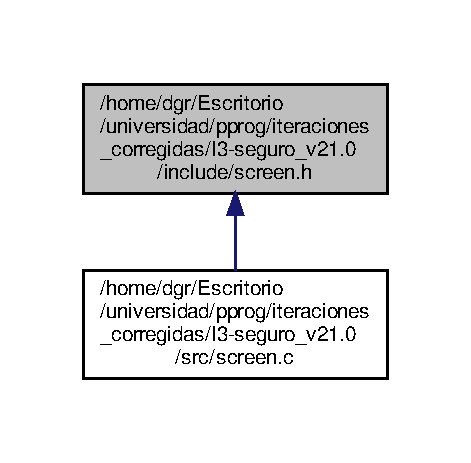
\includegraphics[width=168pt]{screen_8h__dep__incl}
\end{center}
\end{figure}
\subsection*{Macros}
\begin{DoxyCompactItemize}
\item 
\#define \hyperlink{screen_8h_aab63df3ae7b979d59ea0188055ea0763}{S\+C\+R\+E\+E\+N\+\_\+\+M\+A\+X\+\_\+\+S\+TR}~80
\begin{DoxyCompactList}\small\item\em A macro to storage the max number of strings. \end{DoxyCompactList}\end{DoxyCompactItemize}
\subsection*{Typedefs}
\begin{DoxyCompactItemize}
\item 
typedef struct \hyperlink{struct__Area}{\+\_\+\+Area} \hyperlink{screen_8h_acfdfc42f6522d75fa3c16713afde8127}{Area}
\begin{DoxyCompactList}\small\item\em A type definition for a area. \end{DoxyCompactList}\end{DoxyCompactItemize}
\subsection*{Functions}
\begin{DoxyCompactItemize}
\item 
void \hyperlink{screen_8h_a9dbb6c251337c03c078dc330caee48d2}{screen\+\_\+init} ()
\begin{DoxyCompactList}\small\item\em create the background \end{DoxyCompactList}\item 
void \hyperlink{screen_8h_a3d6d82dde2bb4f3ddc4d276dabe313ef}{screen\+\_\+destroy} ()
\begin{DoxyCompactList}\small\item\em free the screen \end{DoxyCompactList}\item 
void \hyperlink{screen_8h_a3eaa0547a956d39b6c55c9593524e0d1}{screen\+\_\+paint} ()
\begin{DoxyCompactList}\small\item\em print in the terminal the background with the data \end{DoxyCompactList}\item 
void \hyperlink{screen_8h_a57b2f852be623dca59255306c1482eb2}{screen\+\_\+gets} (char $\ast$str)
\begin{DoxyCompactList}\small\item\em get the information on the screen \end{DoxyCompactList}\item 
\hyperlink{screen_8h_acfdfc42f6522d75fa3c16713afde8127}{Area} $\ast$ \hyperlink{screen_8h_a194528bec3ed3b57618a8f2df9bea743}{screen\+\_\+area\+\_\+init} (int x, int y, int width, int height)
\begin{DoxyCompactList}\small\item\em create the area of the screen \end{DoxyCompactList}\item 
void \hyperlink{screen_8h_aca5123ed5a7afb75e79c0001e5d1df4f}{screen\+\_\+area\+\_\+destroy} (\hyperlink{screen_8h_acfdfc42f6522d75fa3c16713afde8127}{Area} $\ast$area)
\begin{DoxyCompactList}\small\item\em free the area of the screen \end{DoxyCompactList}\item 
void \hyperlink{screen_8h_a0950dc68cba3d491b909a8abaac1c666}{screen\+\_\+area\+\_\+clear} (\hyperlink{screen_8h_acfdfc42f6522d75fa3c16713afde8127}{Area} $\ast$area)
\begin{DoxyCompactList}\small\item\em clear the area \end{DoxyCompactList}\item 
void \hyperlink{screen_8h_af77fa9df4f7170e1e3bf1c6209b7f0c2}{screen\+\_\+area\+\_\+reset\+\_\+cursor} (\hyperlink{screen_8h_acfdfc42f6522d75fa3c16713afde8127}{Area} $\ast$area)
\begin{DoxyCompactList}\small\item\em reset the cursor \end{DoxyCompactList}\item 
void \hyperlink{screen_8h_a4f4cd4c7899c096d6c90cc33de9a9814}{screen\+\_\+area\+\_\+puts} (\hyperlink{screen_8h_acfdfc42f6522d75fa3c16713afde8127}{Area} $\ast$area, char $\ast$str)
\begin{DoxyCompactList}\small\item\em puts the area \end{DoxyCompactList}\end{DoxyCompactItemize}


\subsection{Detailed Description}
It defines a screen. 

\begin{DoxyAuthor}{Author}
Profesores P\+P\+R\+OG 
\end{DoxyAuthor}
\begin{DoxyVersion}{Version}
1.\+0 
\end{DoxyVersion}
\begin{DoxyDate}{Date}
11-\/01-\/2017 
\end{DoxyDate}
\begin{DoxyCopyright}{Copyright}
G\+NU Public License 
\end{DoxyCopyright}


\subsection{Macro Definition Documentation}
\mbox{\Hypertarget{screen_8h_aab63df3ae7b979d59ea0188055ea0763}\label{screen_8h_aab63df3ae7b979d59ea0188055ea0763}} 
\index{screen.\+h@{screen.\+h}!S\+C\+R\+E\+E\+N\+\_\+\+M\+A\+X\+\_\+\+S\+TR@{S\+C\+R\+E\+E\+N\+\_\+\+M\+A\+X\+\_\+\+S\+TR}}
\index{S\+C\+R\+E\+E\+N\+\_\+\+M\+A\+X\+\_\+\+S\+TR@{S\+C\+R\+E\+E\+N\+\_\+\+M\+A\+X\+\_\+\+S\+TR}!screen.\+h@{screen.\+h}}
\subsubsection{\texorpdfstring{S\+C\+R\+E\+E\+N\+\_\+\+M\+A\+X\+\_\+\+S\+TR}{SCREEN\_MAX\_STR}}
{\footnotesize\ttfamily \#define S\+C\+R\+E\+E\+N\+\_\+\+M\+A\+X\+\_\+\+S\+TR~80}



A macro to storage the max number of strings. 

Details. 

\subsection{Typedef Documentation}
\mbox{\Hypertarget{screen_8h_acfdfc42f6522d75fa3c16713afde8127}\label{screen_8h_acfdfc42f6522d75fa3c16713afde8127}} 
\index{screen.\+h@{screen.\+h}!Area@{Area}}
\index{Area@{Area}!screen.\+h@{screen.\+h}}
\subsubsection{\texorpdfstring{Area}{Area}}
{\footnotesize\ttfamily typedef struct \hyperlink{struct__Area}{\+\_\+\+Area} \hyperlink{screen_8h_acfdfc42f6522d75fa3c16713afde8127}{Area}}



A type definition for a area. 

Details. 

\subsection{Function Documentation}
\mbox{\Hypertarget{screen_8h_a0950dc68cba3d491b909a8abaac1c666}\label{screen_8h_a0950dc68cba3d491b909a8abaac1c666}} 
\index{screen.\+h@{screen.\+h}!screen\+\_\+area\+\_\+clear@{screen\+\_\+area\+\_\+clear}}
\index{screen\+\_\+area\+\_\+clear@{screen\+\_\+area\+\_\+clear}!screen.\+h@{screen.\+h}}
\subsubsection{\texorpdfstring{screen\+\_\+area\+\_\+clear()}{screen\_area\_clear()}}
{\footnotesize\ttfamily void screen\+\_\+area\+\_\+clear (\begin{DoxyParamCaption}\item[{\hyperlink{screen_8h_acfdfc42f6522d75fa3c16713afde8127}{Area} $\ast$}]{area }\end{DoxyParamCaption})}



clear the area 

screen\+\_\+area\+\_\+clear

\begin{DoxyDate}{Date}
13-\/01-\/2015 
\end{DoxyDate}
\begin{DoxyAuthor}{Author}
\+: Instructors of P\+P\+R\+OG
\end{DoxyAuthor}
param area the area we want to modified \mbox{\Hypertarget{screen_8h_aca5123ed5a7afb75e79c0001e5d1df4f}\label{screen_8h_aca5123ed5a7afb75e79c0001e5d1df4f}} 
\index{screen.\+h@{screen.\+h}!screen\+\_\+area\+\_\+destroy@{screen\+\_\+area\+\_\+destroy}}
\index{screen\+\_\+area\+\_\+destroy@{screen\+\_\+area\+\_\+destroy}!screen.\+h@{screen.\+h}}
\subsubsection{\texorpdfstring{screen\+\_\+area\+\_\+destroy()}{screen\_area\_destroy()}}
{\footnotesize\ttfamily void screen\+\_\+area\+\_\+destroy (\begin{DoxyParamCaption}\item[{\hyperlink{screen_8h_acfdfc42f6522d75fa3c16713afde8127}{Area} $\ast$}]{area }\end{DoxyParamCaption})}



free the area of the screen 

screen\+\_\+destroy free a especific space

\begin{DoxyDate}{Date}
13-\/01-\/2015 
\end{DoxyDate}
\begin{DoxyAuthor}{Author}
\+: Instructors of P\+P\+R\+OG
\end{DoxyAuthor}
param area the area we want free \mbox{\Hypertarget{screen_8h_a194528bec3ed3b57618a8f2df9bea743}\label{screen_8h_a194528bec3ed3b57618a8f2df9bea743}} 
\index{screen.\+h@{screen.\+h}!screen\+\_\+area\+\_\+init@{screen\+\_\+area\+\_\+init}}
\index{screen\+\_\+area\+\_\+init@{screen\+\_\+area\+\_\+init}!screen.\+h@{screen.\+h}}
\subsubsection{\texorpdfstring{screen\+\_\+area\+\_\+init()}{screen\_area\_init()}}
{\footnotesize\ttfamily \hyperlink{screen_8h_acfdfc42f6522d75fa3c16713afde8127}{Area}$\ast$ screen\+\_\+area\+\_\+init (\begin{DoxyParamCaption}\item[{int}]{x,  }\item[{int}]{y,  }\item[{int}]{width,  }\item[{int}]{height }\end{DoxyParamCaption})}



create the area of the screen 

screen\+\_\+area\+\_\+init

\begin{DoxyDate}{Date}
13-\/01-\/2015 
\end{DoxyDate}
\begin{DoxyAuthor}{Author}
\+: Instructors of P\+P\+R\+OG
\end{DoxyAuthor}

\begin{DoxyParams}{Parameters}
{\em x} & coordinate x \\
\hline
{\em y} & coordinate y \\
\hline
{\em width} & coordinate width \\
\hline
{\em height} & coordinate height \\
\hline
\end{DoxyParams}
\begin{DoxyReturn}{Returns}
area the area that has been created 
\end{DoxyReturn}
\mbox{\Hypertarget{screen_8h_a4f4cd4c7899c096d6c90cc33de9a9814}\label{screen_8h_a4f4cd4c7899c096d6c90cc33de9a9814}} 
\index{screen.\+h@{screen.\+h}!screen\+\_\+area\+\_\+puts@{screen\+\_\+area\+\_\+puts}}
\index{screen\+\_\+area\+\_\+puts@{screen\+\_\+area\+\_\+puts}!screen.\+h@{screen.\+h}}
\subsubsection{\texorpdfstring{screen\+\_\+area\+\_\+puts()}{screen\_area\_puts()}}
{\footnotesize\ttfamily void screen\+\_\+area\+\_\+puts (\begin{DoxyParamCaption}\item[{\hyperlink{screen_8h_acfdfc42f6522d75fa3c16713afde8127}{Area} $\ast$}]{area,  }\item[{char $\ast$}]{str }\end{DoxyParamCaption})}



puts the area 

screen\+\_\+area\+\_\+puts

\begin{DoxyDate}{Date}
13-\/01-\/2015 
\end{DoxyDate}
\begin{DoxyAuthor}{Author}
\+: Instructors of P\+P\+R\+OG
\end{DoxyAuthor}
param area the area we want to modified param str the string we will use \mbox{\Hypertarget{screen_8h_af77fa9df4f7170e1e3bf1c6209b7f0c2}\label{screen_8h_af77fa9df4f7170e1e3bf1c6209b7f0c2}} 
\index{screen.\+h@{screen.\+h}!screen\+\_\+area\+\_\+reset\+\_\+cursor@{screen\+\_\+area\+\_\+reset\+\_\+cursor}}
\index{screen\+\_\+area\+\_\+reset\+\_\+cursor@{screen\+\_\+area\+\_\+reset\+\_\+cursor}!screen.\+h@{screen.\+h}}
\subsubsection{\texorpdfstring{screen\+\_\+area\+\_\+reset\+\_\+cursor()}{screen\_area\_reset\_cursor()}}
{\footnotesize\ttfamily void screen\+\_\+area\+\_\+reset\+\_\+cursor (\begin{DoxyParamCaption}\item[{\hyperlink{screen_8h_acfdfc42f6522d75fa3c16713afde8127}{Area} $\ast$}]{area }\end{DoxyParamCaption})}



reset the cursor 

screen\+\_\+area\+\_\+reset\+\_\+cursor

\begin{DoxyDate}{Date}
13-\/01-\/2015 
\end{DoxyDate}
\begin{DoxyAuthor}{Author}
\+: Instructors of P\+P\+R\+OG
\end{DoxyAuthor}
param area the area we want to modified \mbox{\Hypertarget{screen_8h_a3d6d82dde2bb4f3ddc4d276dabe313ef}\label{screen_8h_a3d6d82dde2bb4f3ddc4d276dabe313ef}} 
\index{screen.\+h@{screen.\+h}!screen\+\_\+destroy@{screen\+\_\+destroy}}
\index{screen\+\_\+destroy@{screen\+\_\+destroy}!screen.\+h@{screen.\+h}}
\subsubsection{\texorpdfstring{screen\+\_\+destroy()}{screen\_destroy()}}
{\footnotesize\ttfamily void screen\+\_\+destroy (\begin{DoxyParamCaption}{ }\end{DoxyParamCaption})}



free the screen 

screen\+\_\+destroy free a especific space

\begin{DoxyDate}{Date}
13-\/01-\/2015 
\end{DoxyDate}
\begin{DoxyAuthor}{Author}
\+: Instructors of P\+P\+R\+OG 
\end{DoxyAuthor}
\mbox{\Hypertarget{screen_8h_a57b2f852be623dca59255306c1482eb2}\label{screen_8h_a57b2f852be623dca59255306c1482eb2}} 
\index{screen.\+h@{screen.\+h}!screen\+\_\+gets@{screen\+\_\+gets}}
\index{screen\+\_\+gets@{screen\+\_\+gets}!screen.\+h@{screen.\+h}}
\subsubsection{\texorpdfstring{screen\+\_\+gets()}{screen\_gets()}}
{\footnotesize\ttfamily void screen\+\_\+gets (\begin{DoxyParamCaption}\item[{char $\ast$}]{str }\end{DoxyParamCaption})}



get the information on the screen 

screen\+\_\+gets

\begin{DoxyDate}{Date}
13-\/01-\/2015 
\end{DoxyDate}
\begin{DoxyAuthor}{Author}
\+: Instructors of P\+P\+R\+OG 
\end{DoxyAuthor}
\mbox{\Hypertarget{screen_8h_a9dbb6c251337c03c078dc330caee48d2}\label{screen_8h_a9dbb6c251337c03c078dc330caee48d2}} 
\index{screen.\+h@{screen.\+h}!screen\+\_\+init@{screen\+\_\+init}}
\index{screen\+\_\+init@{screen\+\_\+init}!screen.\+h@{screen.\+h}}
\subsubsection{\texorpdfstring{screen\+\_\+init()}{screen\_init()}}
{\footnotesize\ttfamily void screen\+\_\+init (\begin{DoxyParamCaption}{ }\end{DoxyParamCaption})}



create the background 

screen\+\_\+init

\begin{DoxyDate}{Date}
13-\/01-\/2015 
\end{DoxyDate}
\begin{DoxyAuthor}{Author}
\+: Instructors of P\+P\+R\+OG 
\end{DoxyAuthor}
\mbox{\Hypertarget{screen_8h_a3eaa0547a956d39b6c55c9593524e0d1}\label{screen_8h_a3eaa0547a956d39b6c55c9593524e0d1}} 
\index{screen.\+h@{screen.\+h}!screen\+\_\+paint@{screen\+\_\+paint}}
\index{screen\+\_\+paint@{screen\+\_\+paint}!screen.\+h@{screen.\+h}}
\subsubsection{\texorpdfstring{screen\+\_\+paint()}{screen\_paint()}}
{\footnotesize\ttfamily void screen\+\_\+paint (\begin{DoxyParamCaption}{ }\end{DoxyParamCaption})}



print in the terminal the background with the data 

screen\+\_\+paint

\begin{DoxyDate}{Date}
13-\/01-\/2015 
\end{DoxyDate}
\begin{DoxyAuthor}{Author}
\+: Instructors of P\+P\+R\+OG 
\end{DoxyAuthor}

\hypertarget{set_8h}{}\section{include/set.h File Reference}
\label{set_8h}\index{include/set.\+h@{include/set.\+h}}


It defines the set interface for each command.  


{\ttfamily \#include \char`\"{}../include/types.\+h\char`\"{}}\newline
{\ttfamily \#include $<$stdio.\+h$>$}\newline
Include dependency graph for set.\+h\+:\nopagebreak
\begin{figure}[H]
\begin{center}
\leavevmode
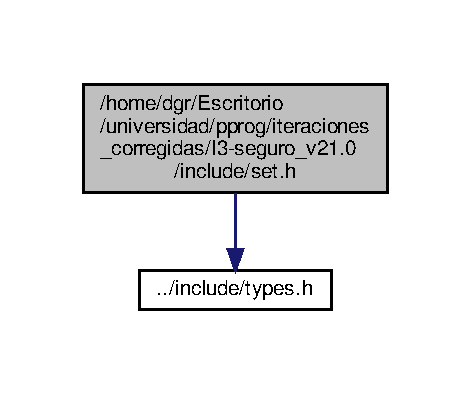
\includegraphics[width=236pt]{set_8h__incl}
\end{center}
\end{figure}
This graph shows which files directly or indirectly include this file\+:\nopagebreak
\begin{figure}[H]
\begin{center}
\leavevmode
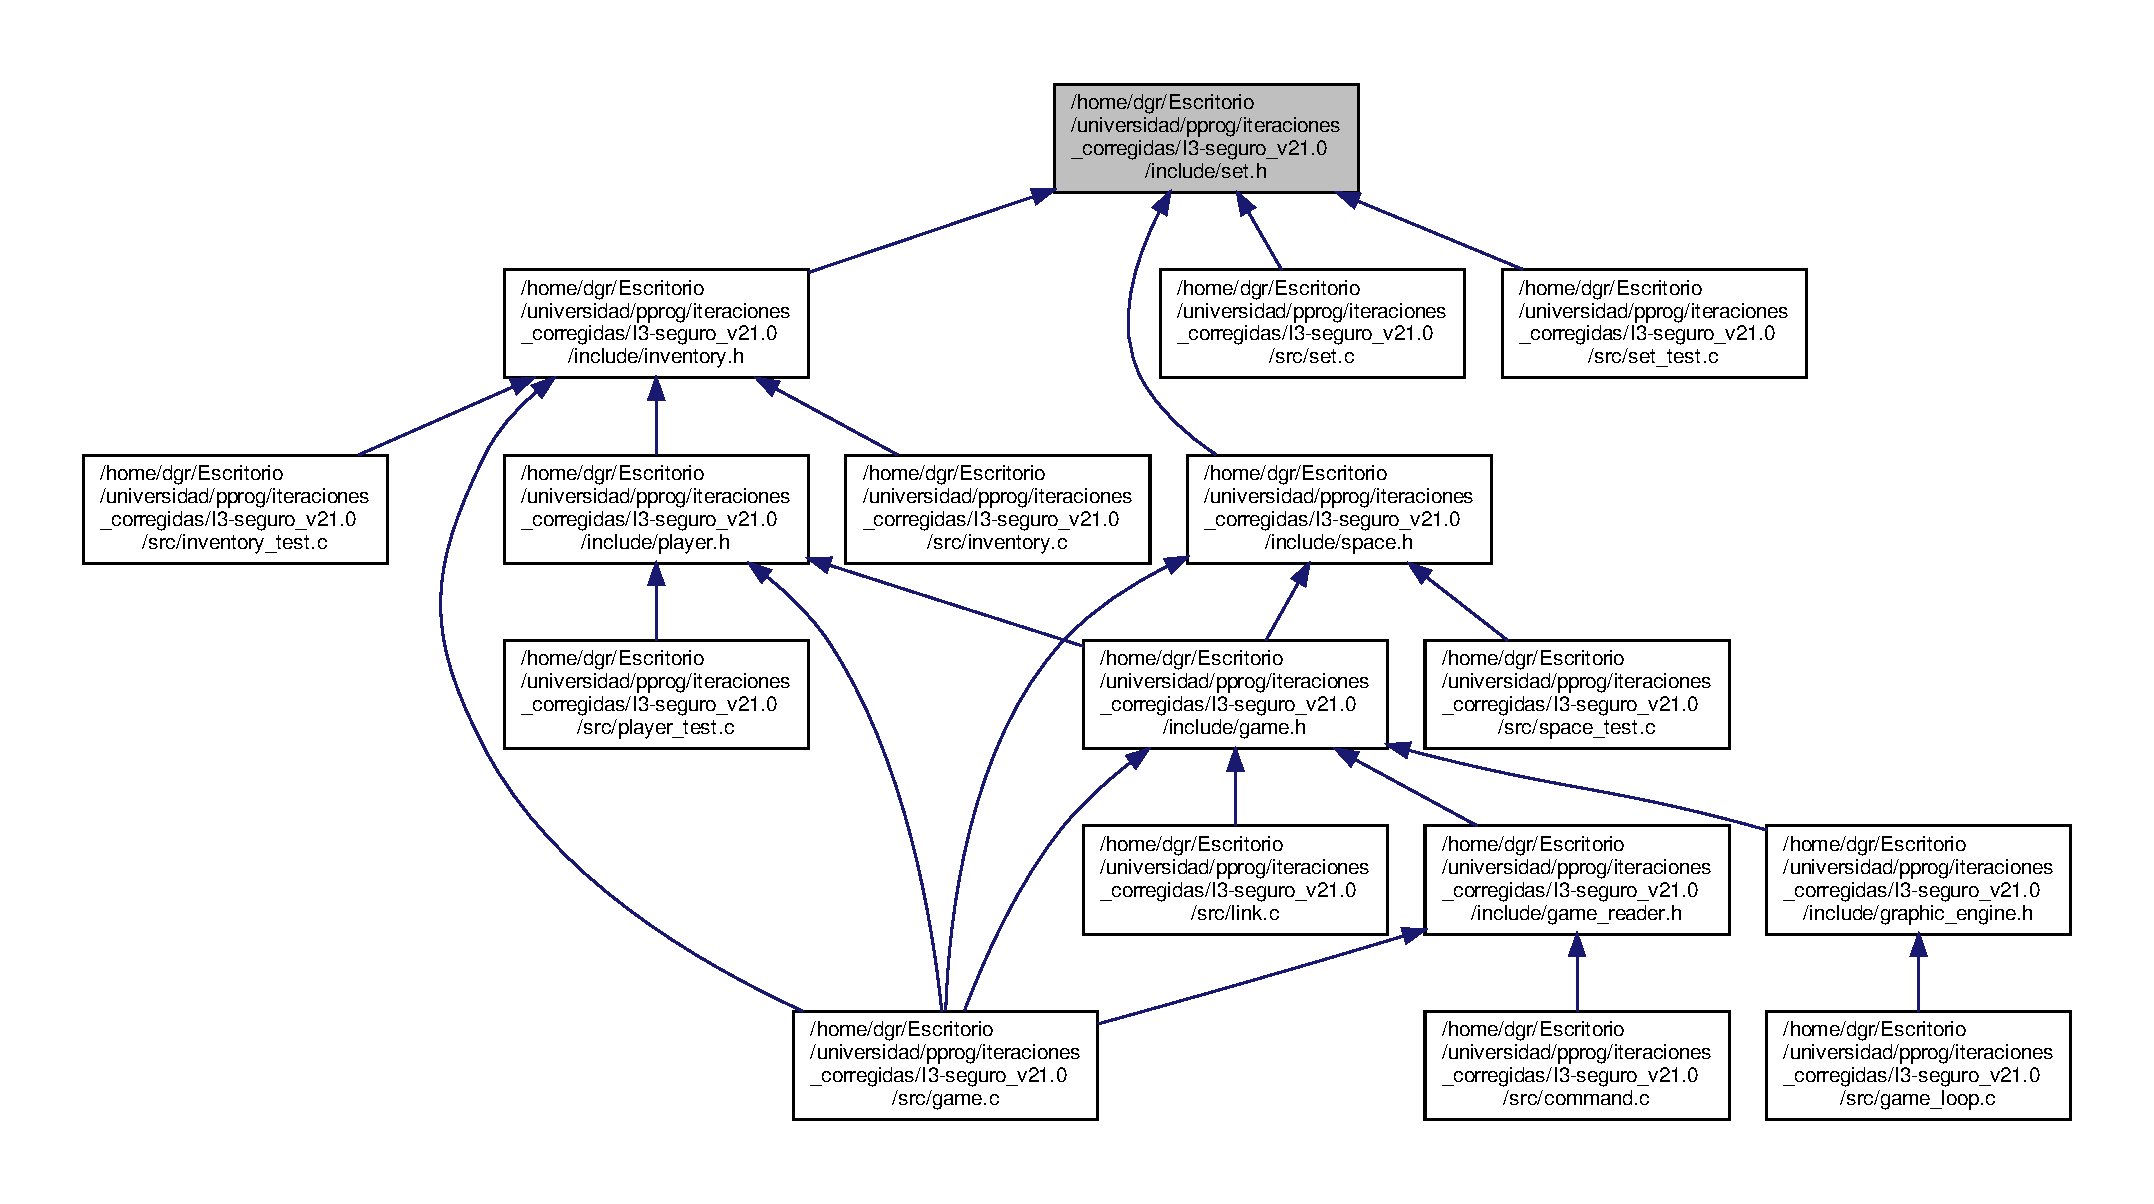
\includegraphics[width=350pt]{set_8h__dep__incl}
\end{center}
\end{figure}
\subsection*{Typedefs}
\begin{DoxyCompactItemize}
\item 
typedef struct \hyperlink{struct__Set}{\+\_\+\+Set} \hyperlink{set_8h_a6d3b7f7c92cbb4577ef3ef7ddbf93161}{Set}
\begin{DoxyCompactList}\small\item\em A type definition for a set. \end{DoxyCompactList}\end{DoxyCompactItemize}
\subsection*{Functions}
\begin{DoxyCompactItemize}
\item 
\hyperlink{set_8h_a6d3b7f7c92cbb4577ef3ef7ddbf93161}{Set} $\ast$ \hyperlink{set_8h_abcc73b7ad3913fc92dd95d366c9c8687}{set\+\_\+create} ()
\begin{DoxyCompactList}\small\item\em Create the set. \end{DoxyCompactList}\item 
\hyperlink{types_8h_a32c27cc471df37f4fc818d65de0a56c4}{S\+T\+A\+T\+US} \hyperlink{set_8h_a17fa263a49d6fe209c040e9ca5e0132a}{set\+\_\+destroy} (\hyperlink{set_8h_a6d3b7f7c92cbb4577ef3ef7ddbf93161}{Set} $\ast$set)
\begin{DoxyCompactList}\small\item\em Destroy the set. \end{DoxyCompactList}\item 
\hyperlink{types_8h_a32c27cc471df37f4fc818d65de0a56c4}{S\+T\+A\+T\+US} \hyperlink{set_8h_a214235069ee276ad9bceb2c66e56bfe1}{set\+\_\+add} (\hyperlink{set_8h_a6d3b7f7c92cbb4577ef3ef7ddbf93161}{Set} $\ast$set, \hyperlink{types_8h_a845e604fb28f7e3d97549da3448149d3}{Id} id)
\begin{DoxyCompactList}\small\item\em Add element to the set. \end{DoxyCompactList}\item 
void \hyperlink{set_8h_ab7cd9162335d346f5457eef63692a96b}{set\+\_\+print} (F\+I\+LE $\ast$f, \hyperlink{set_8h_a6d3b7f7c92cbb4577ef3ef7ddbf93161}{Set} $\ast$set)
\begin{DoxyCompactList}\small\item\em print the elements of the set \end{DoxyCompactList}\item 
int \hyperlink{set_8h_a62a3c1e0de34be5b9b2f5161a430f090}{set\+\_\+get\+\_\+num} (\hyperlink{set_8h_a6d3b7f7c92cbb4577ef3ef7ddbf93161}{Set} $\ast$set)
\begin{DoxyCompactList}\small\item\em return the namber of id allocated in a set \end{DoxyCompactList}\item 
int \hyperlink{set_8h_a565a873b0d50133d4c48319e8b6b13d9}{set\+\_\+find\+\_\+index} (\hyperlink{set_8h_a6d3b7f7c92cbb4577ef3ef7ddbf93161}{Set} $\ast$set, \hyperlink{types_8h_a845e604fb28f7e3d97549da3448149d3}{Id} id)
\begin{DoxyCompactList}\small\item\em return the index of and id \end{DoxyCompactList}\item 
\hyperlink{types_8h_a32c27cc471df37f4fc818d65de0a56c4}{S\+T\+A\+T\+US} \hyperlink{set_8h_a7132be7ebdf9b2d3b1f23895a59a25df}{set\+\_\+dell} (\hyperlink{set_8h_a6d3b7f7c92cbb4577ef3ef7ddbf93161}{Set} $\ast$set, \hyperlink{types_8h_a845e604fb28f7e3d97549da3448149d3}{Id} id)
\begin{DoxyCompactList}\small\item\em remove or delete an id in a set \end{DoxyCompactList}\item 
\hyperlink{types_8h_a845e604fb28f7e3d97549da3448149d3}{Id} \hyperlink{set_8h_a37b5d27dabd419279fe1eddc40cec0fa}{set\+\_\+get\+\_\+id\+\_\+at\+\_\+position} (\hyperlink{set_8h_a6d3b7f7c92cbb4577ef3ef7ddbf93161}{Set} $\ast$set, int position)
\begin{DoxyCompactList}\small\item\em returns the id of the indicated position \end{DoxyCompactList}\item 
\hyperlink{types_8h_a32c27cc471df37f4fc818d65de0a56c4}{S\+T\+A\+T\+US} \hyperlink{set_8h_ac996936009c685a89fdc26c27a9b1874}{set\+\_\+update} (\hyperlink{set_8h_a6d3b7f7c92cbb4577ef3ef7ddbf93161}{Set} $\ast$original, \hyperlink{set_8h_a6d3b7f7c92cbb4577ef3ef7ddbf93161}{Set} $\ast$final)
\begin{DoxyCompactList}\small\item\em update a set with a new set \end{DoxyCompactList}\end{DoxyCompactItemize}


\subsection{Detailed Description}
It defines the set interface for each command. 

\begin{DoxyAuthor}{Author}
David Teófilo Garitagoitia Romero 
\end{DoxyAuthor}
\begin{DoxyVersion}{Version}
1.\+0 
\end{DoxyVersion}
\begin{DoxyDate}{Date}
20-\/02-\/2020 
\end{DoxyDate}
\begin{DoxyCopyright}{Copyright}
G\+NU Public License 
\end{DoxyCopyright}


\subsection{Typedef Documentation}
\mbox{\Hypertarget{set_8h_a6d3b7f7c92cbb4577ef3ef7ddbf93161}\label{set_8h_a6d3b7f7c92cbb4577ef3ef7ddbf93161}} 
\index{set.\+h@{set.\+h}!Set@{Set}}
\index{Set@{Set}!set.\+h@{set.\+h}}
\subsubsection{\texorpdfstring{Set}{Set}}
{\footnotesize\ttfamily typedef struct \hyperlink{struct__Set}{\+\_\+\+Set} \hyperlink{set_8h_a6d3b7f7c92cbb4577ef3ef7ddbf93161}{Set}}



A type definition for a set. 

Details. 

\subsection{Function Documentation}
\mbox{\Hypertarget{set_8h_a214235069ee276ad9bceb2c66e56bfe1}\label{set_8h_a214235069ee276ad9bceb2c66e56bfe1}} 
\index{set.\+h@{set.\+h}!set\+\_\+add@{set\+\_\+add}}
\index{set\+\_\+add@{set\+\_\+add}!set.\+h@{set.\+h}}
\subsubsection{\texorpdfstring{set\+\_\+add()}{set\_add()}}
{\footnotesize\ttfamily \hyperlink{types_8h_a32c27cc471df37f4fc818d65de0a56c4}{S\+T\+A\+T\+US} set\+\_\+add (\begin{DoxyParamCaption}\item[{\hyperlink{set_8h_a6d3b7f7c92cbb4577ef3ef7ddbf93161}{Set} $\ast$}]{set,  }\item[{\hyperlink{types_8h_a845e604fb28f7e3d97549da3448149d3}{Id}}]{id }\end{DoxyParamCaption})}



Add element to the set. 

set\+\_\+add add an element to the set

\begin{DoxyDate}{Date}
20-\/02-\/2020 
\end{DoxyDate}
\begin{DoxyAuthor}{Author}
David Teófilo Garitagoitia Romero
\end{DoxyAuthor}

\begin{DoxyParams}{Parameters}
{\em set} & the addres os the set in which you want to add an element \\
\hline
{\em id} & the id of the element that you want to add \\
\hline
\end{DoxyParams}
\begin{DoxyReturn}{Returns}
Ok if there was no problem, 
\end{DoxyReturn}
\mbox{\Hypertarget{set_8h_abcc73b7ad3913fc92dd95d366c9c8687}\label{set_8h_abcc73b7ad3913fc92dd95d366c9c8687}} 
\index{set.\+h@{set.\+h}!set\+\_\+create@{set\+\_\+create}}
\index{set\+\_\+create@{set\+\_\+create}!set.\+h@{set.\+h}}
\subsubsection{\texorpdfstring{set\+\_\+create()}{set\_create()}}
{\footnotesize\ttfamily \hyperlink{set_8h_a6d3b7f7c92cbb4577ef3ef7ddbf93161}{Set}$\ast$ set\+\_\+create (\begin{DoxyParamCaption}{ }\end{DoxyParamCaption})}



Create the set. 

set\+\_\+create Create a new set

\begin{DoxyDate}{Date}
20-\/02-\/2020 
\end{DoxyDate}
\begin{DoxyAuthor}{Author}
David Teófilo Garitagoitia Romero 
\end{DoxyAuthor}
\begin{DoxyReturn}{Returns}
the new set that has been created 
\end{DoxyReturn}
\mbox{\Hypertarget{set_8h_a7132be7ebdf9b2d3b1f23895a59a25df}\label{set_8h_a7132be7ebdf9b2d3b1f23895a59a25df}} 
\index{set.\+h@{set.\+h}!set\+\_\+dell@{set\+\_\+dell}}
\index{set\+\_\+dell@{set\+\_\+dell}!set.\+h@{set.\+h}}
\subsubsection{\texorpdfstring{set\+\_\+dell()}{set\_dell()}}
{\footnotesize\ttfamily \hyperlink{types_8h_a32c27cc471df37f4fc818d65de0a56c4}{S\+T\+A\+T\+US} set\+\_\+dell (\begin{DoxyParamCaption}\item[{\hyperlink{set_8h_a6d3b7f7c92cbb4577ef3ef7ddbf93161}{Set} $\ast$}]{set,  }\item[{\hyperlink{types_8h_a845e604fb28f7e3d97549da3448149d3}{Id}}]{id }\end{DoxyParamCaption})}



remove or delete an id in a set 

set\+\_\+dell

\begin{DoxyDate}{Date}
22-\/02-\/2020 
\end{DoxyDate}
\begin{DoxyAuthor}{Author}
\+: David Teófilo Garitagoitia Romero
\end{DoxyAuthor}

\begin{DoxyParams}{Parameters}
{\em set} & the set which contains the id \\
\hline
{\em id} & the id that you want to delete \\
\hline
\end{DoxyParams}
\begin{DoxyReturn}{Returns}

\end{DoxyReturn}
\mbox{\Hypertarget{set_8h_a17fa263a49d6fe209c040e9ca5e0132a}\label{set_8h_a17fa263a49d6fe209c040e9ca5e0132a}} 
\index{set.\+h@{set.\+h}!set\+\_\+destroy@{set\+\_\+destroy}}
\index{set\+\_\+destroy@{set\+\_\+destroy}!set.\+h@{set.\+h}}
\subsubsection{\texorpdfstring{set\+\_\+destroy()}{set\_destroy()}}
{\footnotesize\ttfamily \hyperlink{types_8h_a32c27cc471df37f4fc818d65de0a56c4}{S\+T\+A\+T\+US} set\+\_\+destroy (\begin{DoxyParamCaption}\item[{\hyperlink{set_8h_a6d3b7f7c92cbb4577ef3ef7ddbf93161}{Set} $\ast$}]{set }\end{DoxyParamCaption})}



Destroy the set. 

set\+\_\+destroy a set

\begin{DoxyDate}{Date}
20-\/02-\/2020 
\end{DoxyDate}
\begin{DoxyAuthor}{Author}
David Teófilo Garitagoitia Romero
\end{DoxyAuthor}

\begin{DoxyParams}{Parameters}
{\em set} & the addres of the set which you want to print \\
\hline
\end{DoxyParams}
\begin{DoxyReturn}{Returns}
Ok if there was no problem, 
\end{DoxyReturn}
\mbox{\Hypertarget{set_8h_a565a873b0d50133d4c48319e8b6b13d9}\label{set_8h_a565a873b0d50133d4c48319e8b6b13d9}} 
\index{set.\+h@{set.\+h}!set\+\_\+find\+\_\+index@{set\+\_\+find\+\_\+index}}
\index{set\+\_\+find\+\_\+index@{set\+\_\+find\+\_\+index}!set.\+h@{set.\+h}}
\subsubsection{\texorpdfstring{set\+\_\+find\+\_\+index()}{set\_find\_index()}}
{\footnotesize\ttfamily int set\+\_\+find\+\_\+index (\begin{DoxyParamCaption}\item[{\hyperlink{set_8h_a6d3b7f7c92cbb4577ef3ef7ddbf93161}{Set} $\ast$}]{set,  }\item[{\hyperlink{types_8h_a845e604fb28f7e3d97549da3448149d3}{Id}}]{id }\end{DoxyParamCaption})}



return the index of and id 

set\+\_\+find\+\_\+index

\begin{DoxyDate}{Date}
26-\/02-\/2020 
\end{DoxyDate}
\begin{DoxyAuthor}{Author}
\+: David Teófilo Garitagoitia Romero
\end{DoxyAuthor}

\begin{DoxyParams}{Parameters}
{\em set} & the set which contains the id \\
\hline
{\em id} & the id that you want to know their position \\
\hline
\end{DoxyParams}
\begin{DoxyReturn}{Returns}

\end{DoxyReturn}
\mbox{\Hypertarget{set_8h_a37b5d27dabd419279fe1eddc40cec0fa}\label{set_8h_a37b5d27dabd419279fe1eddc40cec0fa}} 
\index{set.\+h@{set.\+h}!set\+\_\+get\+\_\+id\+\_\+at\+\_\+position@{set\+\_\+get\+\_\+id\+\_\+at\+\_\+position}}
\index{set\+\_\+get\+\_\+id\+\_\+at\+\_\+position@{set\+\_\+get\+\_\+id\+\_\+at\+\_\+position}!set.\+h@{set.\+h}}
\subsubsection{\texorpdfstring{set\+\_\+get\+\_\+id\+\_\+at\+\_\+position()}{set\_get\_id\_at\_position()}}
{\footnotesize\ttfamily \hyperlink{types_8h_a845e604fb28f7e3d97549da3448149d3}{Id} set\+\_\+get\+\_\+id\+\_\+at\+\_\+position (\begin{DoxyParamCaption}\item[{\hyperlink{set_8h_a6d3b7f7c92cbb4577ef3ef7ddbf93161}{Set} $\ast$}]{set,  }\item[{int}]{position }\end{DoxyParamCaption})}



returns the id of the indicated position 

set\+\_\+get\+\_\+id\+\_\+at\+\_\+position

\begin{DoxyDate}{Date}
26-\/02-\/2020 
\end{DoxyDate}
\begin{DoxyAuthor}{Author}
\+: David Teófilo Garitagoitia Romero
\end{DoxyAuthor}

\begin{DoxyParams}{Parameters}
{\em set} & the set which contains the id \\
\hline
{\em position} & the position of the id \\
\hline
\end{DoxyParams}
\begin{DoxyReturn}{Returns}

\end{DoxyReturn}
\mbox{\Hypertarget{set_8h_a62a3c1e0de34be5b9b2f5161a430f090}\label{set_8h_a62a3c1e0de34be5b9b2f5161a430f090}} 
\index{set.\+h@{set.\+h}!set\+\_\+get\+\_\+num@{set\+\_\+get\+\_\+num}}
\index{set\+\_\+get\+\_\+num@{set\+\_\+get\+\_\+num}!set.\+h@{set.\+h}}
\subsubsection{\texorpdfstring{set\+\_\+get\+\_\+num()}{set\_get\_num()}}
{\footnotesize\ttfamily int set\+\_\+get\+\_\+num (\begin{DoxyParamCaption}\item[{\hyperlink{set_8h_a6d3b7f7c92cbb4577ef3ef7ddbf93161}{Set} $\ast$}]{set }\end{DoxyParamCaption})}



return the namber of id allocated in a set 

set\+\_\+get\+\_\+num

\begin{DoxyDate}{Date}
20-\/02-\/2020 
\end{DoxyDate}
\begin{DoxyAuthor}{Author}
\+: David Teófilo Garitagoitia Romero
\end{DoxyAuthor}

\begin{DoxyParams}{Parameters}
{\em set} & the set that you want to know their number of ids \\
\hline
\end{DoxyParams}
\begin{DoxyReturn}{Returns}

\end{DoxyReturn}
\mbox{\Hypertarget{set_8h_ab7cd9162335d346f5457eef63692a96b}\label{set_8h_ab7cd9162335d346f5457eef63692a96b}} 
\index{set.\+h@{set.\+h}!set\+\_\+print@{set\+\_\+print}}
\index{set\+\_\+print@{set\+\_\+print}!set.\+h@{set.\+h}}
\subsubsection{\texorpdfstring{set\+\_\+print()}{set\_print()}}
{\footnotesize\ttfamily void set\+\_\+print (\begin{DoxyParamCaption}\item[{F\+I\+LE $\ast$}]{f,  }\item[{\hyperlink{set_8h_a6d3b7f7c92cbb4577ef3ef7ddbf93161}{Set} $\ast$}]{set }\end{DoxyParamCaption})}



print the elements of the set 

set\+\_\+print

\begin{DoxyDate}{Date}
20-\/02-\/2020 
\end{DoxyDate}
\begin{DoxyAuthor}{Author}
\+: David Teófilo Garitagoitia Romero
\end{DoxyAuthor}

\begin{DoxyParams}{Parameters}
{\em set} & the set you want to print \\
\hline
{\em f} & in which you want to print and set which have the elements \\
\hline
\end{DoxyParams}
\begin{DoxyReturn}{Returns}

\end{DoxyReturn}
\mbox{\Hypertarget{set_8h_ac996936009c685a89fdc26c27a9b1874}\label{set_8h_ac996936009c685a89fdc26c27a9b1874}} 
\index{set.\+h@{set.\+h}!set\+\_\+update@{set\+\_\+update}}
\index{set\+\_\+update@{set\+\_\+update}!set.\+h@{set.\+h}}
\subsubsection{\texorpdfstring{set\+\_\+update()}{set\_update()}}
{\footnotesize\ttfamily \hyperlink{types_8h_a32c27cc471df37f4fc818d65de0a56c4}{S\+T\+A\+T\+US} set\+\_\+update (\begin{DoxyParamCaption}\item[{\hyperlink{set_8h_a6d3b7f7c92cbb4577ef3ef7ddbf93161}{Set} $\ast$}]{original,  }\item[{\hyperlink{set_8h_a6d3b7f7c92cbb4577ef3ef7ddbf93161}{Set} $\ast$}]{final }\end{DoxyParamCaption})}



update a set with a new set 

set\+\_\+update

\begin{DoxyDate}{Date}
26-\/04-\/2020 
\end{DoxyDate}
\begin{DoxyAuthor}{Author}
\+: David Teófilo Garitagoitia Romero
\end{DoxyAuthor}

\begin{DoxyParams}{Parameters}
{\em original} & the set which you want to update \\
\hline
{\em final} & the set with the new info \\
\hline
\end{DoxyParams}
\begin{DoxyReturn}{Returns}

\end{DoxyReturn}

\hypertarget{set__test_8h}{}\section{/home/dgr/\+Escritorio/universidad/pprog/iteraciones\+\_\+corregidas/\+I3-\/seguro\+\_\+v21.0/include/set\+\_\+test.h File Reference}
\label{set__test_8h}\index{/home/dgr/\+Escritorio/universidad/pprog/iteraciones\+\_\+corregidas/\+I3-\/seguro\+\_\+v21.\+0/include/set\+\_\+test.\+h@{/home/dgr/\+Escritorio/universidad/pprog/iteraciones\+\_\+corregidas/\+I3-\/seguro\+\_\+v21.\+0/include/set\+\_\+test.\+h}}


It declares the tests for the set module.  


This graph shows which files directly or indirectly include this file\+:
\nopagebreak
\begin{figure}[H]
\begin{center}
\leavevmode
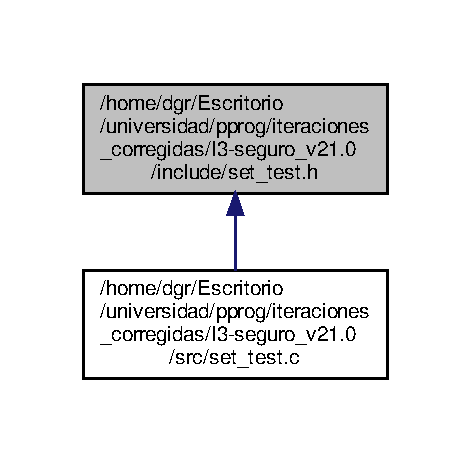
\includegraphics[width=226pt]{set__test_8h__dep__incl}
\end{center}
\end{figure}
\subsection*{Functions}
\begin{DoxyCompactItemize}
\item 
void \hyperlink{set__test_8h_a6f654ab4b44e8a9b9cedfb78c378a5d7}{test1\+\_\+set\+\_\+create} ()
\item 
void \hyperlink{set__test_8h_abed3d273788e23fc31ae7f5ed59277b9}{test2\+\_\+set\+\_\+create} ()
\item 
void \hyperlink{set__test_8h_a014ebe1b46af5ea318143fc61894d9c0}{test1\+\_\+set\+\_\+add} ()
\item 
void \hyperlink{set__test_8h_ab09827322a313bf97b9757c98c2bdbb0}{test2\+\_\+set\+\_\+add} ()
\item 
void \hyperlink{set__test_8h_af36fe01c5b5a8c7c58706f7fe4841d27}{test1\+\_\+set\+\_\+dell} ()
\item 
void \hyperlink{set__test_8h_a9fbb61e5eea38d7417eb5ef64eb766f2}{test2\+\_\+set\+\_\+dell} ()
\item 
void \hyperlink{set__test_8h_a3891f28cf2daa0da4811e667cac542cb}{test3\+\_\+set\+\_\+dell} ()
\item 
void \hyperlink{set__test_8h_ae1ad6c5f19a1a960ae5ccfa970c3d285}{test1\+\_\+set\+\_\+get\+\_\+num} ()
\item 
void \hyperlink{set__test_8h_a6959f1b2ac1f7aacdbb199a9028845ac}{test2\+\_\+set\+\_\+get\+\_\+num} ()
\item 
void \hyperlink{set__test_8h_a67852c621c997ab9a5b1ad30f7bf9f1b}{test1\+\_\+set\+\_\+find\+\_\+index} ()
\item 
void \hyperlink{set__test_8h_ab12db9af55352dff078faf323c25bbd8}{test2\+\_\+set\+\_\+find\+\_\+index} ()
\item 
void \hyperlink{set__test_8h_a7dbb3115868eefb7e52d606f05e3187e}{test1\+\_\+set\+\_\+get\+\_\+id\+\_\+at\+\_\+position} ()
\item 
void \hyperlink{set__test_8h_a4151e3cdda9104e29200e4662be27313}{test2\+\_\+set\+\_\+get\+\_\+id\+\_\+at\+\_\+position} ()
\end{DoxyCompactItemize}


\subsection{Detailed Description}
It declares the tests for the set module. 

\begin{DoxyAuthor}{Author}
Daniel Cerrato Sánchez 
\end{DoxyAuthor}
\begin{DoxyVersion}{Version}
1.\+0 
\end{DoxyVersion}
\begin{DoxyDate}{Date}
08-\/06-\/2020 
\end{DoxyDate}
\begin{DoxyCopyright}{Copyright}
G\+NU Public License 
\end{DoxyCopyright}


\subsection{Function Documentation}
\mbox{\Hypertarget{set__test_8h_a014ebe1b46af5ea318143fc61894d9c0}\label{set__test_8h_a014ebe1b46af5ea318143fc61894d9c0}} 
\index{set\+\_\+test.\+h@{set\+\_\+test.\+h}!test1\+\_\+set\+\_\+add@{test1\+\_\+set\+\_\+add}}
\index{test1\+\_\+set\+\_\+add@{test1\+\_\+set\+\_\+add}!set\+\_\+test.\+h@{set\+\_\+test.\+h}}
\subsubsection{\texorpdfstring{test1\+\_\+set\+\_\+add()}{test1\_set\_add()}}
{\footnotesize\ttfamily void test1\+\_\+set\+\_\+add (\begin{DoxyParamCaption}{ }\end{DoxyParamCaption})}

\begin{DoxyRefDesc}{Test}
\item[\hyperlink{test__test000140}{Test}]Test the function of adding an id to the set \end{DoxyRefDesc}
\begin{DoxyPrecond}{Precondition}
The set is a non-\/\+N\+U\+LL pointer passing a correct id 
\end{DoxyPrecond}
\begin{DoxyPostcond}{Postcondition}
The output must be OK 
\end{DoxyPostcond}
\mbox{\Hypertarget{set__test_8h_a6f654ab4b44e8a9b9cedfb78c378a5d7}\label{set__test_8h_a6f654ab4b44e8a9b9cedfb78c378a5d7}} 
\index{set\+\_\+test.\+h@{set\+\_\+test.\+h}!test1\+\_\+set\+\_\+create@{test1\+\_\+set\+\_\+create}}
\index{test1\+\_\+set\+\_\+create@{test1\+\_\+set\+\_\+create}!set\+\_\+test.\+h@{set\+\_\+test.\+h}}
\subsubsection{\texorpdfstring{test1\+\_\+set\+\_\+create()}{test1\_set\_create()}}
{\footnotesize\ttfamily void test1\+\_\+set\+\_\+create (\begin{DoxyParamCaption}{ }\end{DoxyParamCaption})}

\begin{DoxyRefDesc}{Test}
\item[\hyperlink{test__test000138}{Test}]Test the set creation function \end{DoxyRefDesc}
\begin{DoxyPrecond}{Precondition}
No arguments needed 
\end{DoxyPrecond}
\begin{DoxyPostcond}{Postcondition}
A non-\/null pointer to the created set 
\end{DoxyPostcond}
\mbox{\Hypertarget{set__test_8h_af36fe01c5b5a8c7c58706f7fe4841d27}\label{set__test_8h_af36fe01c5b5a8c7c58706f7fe4841d27}} 
\index{set\+\_\+test.\+h@{set\+\_\+test.\+h}!test1\+\_\+set\+\_\+dell@{test1\+\_\+set\+\_\+dell}}
\index{test1\+\_\+set\+\_\+dell@{test1\+\_\+set\+\_\+dell}!set\+\_\+test.\+h@{set\+\_\+test.\+h}}
\subsubsection{\texorpdfstring{test1\+\_\+set\+\_\+dell()}{test1\_set\_dell()}}
{\footnotesize\ttfamily void test1\+\_\+set\+\_\+dell (\begin{DoxyParamCaption}{ }\end{DoxyParamCaption})}

\begin{DoxyRefDesc}{Test}
\item[\hyperlink{test__test000142}{Test}]Test the function of deleting an id to the set \end{DoxyRefDesc}
\begin{DoxyPrecond}{Precondition}
The set is a non-\/\+N\+U\+LL pointer with a correct id, a correct id is searched 
\end{DoxyPrecond}
\begin{DoxyPostcond}{Postcondition}
The output must be OK 
\end{DoxyPostcond}
\mbox{\Hypertarget{set__test_8h_a67852c621c997ab9a5b1ad30f7bf9f1b}\label{set__test_8h_a67852c621c997ab9a5b1ad30f7bf9f1b}} 
\index{set\+\_\+test.\+h@{set\+\_\+test.\+h}!test1\+\_\+set\+\_\+find\+\_\+index@{test1\+\_\+set\+\_\+find\+\_\+index}}
\index{test1\+\_\+set\+\_\+find\+\_\+index@{test1\+\_\+set\+\_\+find\+\_\+index}!set\+\_\+test.\+h@{set\+\_\+test.\+h}}
\subsubsection{\texorpdfstring{test1\+\_\+set\+\_\+find\+\_\+index()}{test1\_set\_find\_index()}}
{\footnotesize\ttfamily void test1\+\_\+set\+\_\+find\+\_\+index (\begin{DoxyParamCaption}{ }\end{DoxyParamCaption})}

\begin{DoxyRefDesc}{Test}
\item[\hyperlink{test__test000147}{Test}]Test the function to get the position of an id in the set \end{DoxyRefDesc}
\begin{DoxyPrecond}{Precondition}
The set is a non-\/\+N\+U\+LL pointer with at least one id, a correct id is searched 
\end{DoxyPrecond}
\begin{DoxyPostcond}{Postcondition}
The output must be the position of that id in the set 
\end{DoxyPostcond}
\mbox{\Hypertarget{set__test_8h_a7dbb3115868eefb7e52d606f05e3187e}\label{set__test_8h_a7dbb3115868eefb7e52d606f05e3187e}} 
\index{set\+\_\+test.\+h@{set\+\_\+test.\+h}!test1\+\_\+set\+\_\+get\+\_\+id\+\_\+at\+\_\+position@{test1\+\_\+set\+\_\+get\+\_\+id\+\_\+at\+\_\+position}}
\index{test1\+\_\+set\+\_\+get\+\_\+id\+\_\+at\+\_\+position@{test1\+\_\+set\+\_\+get\+\_\+id\+\_\+at\+\_\+position}!set\+\_\+test.\+h@{set\+\_\+test.\+h}}
\subsubsection{\texorpdfstring{test1\+\_\+set\+\_\+get\+\_\+id\+\_\+at\+\_\+position()}{test1\_set\_get\_id\_at\_position()}}
{\footnotesize\ttfamily void test1\+\_\+set\+\_\+get\+\_\+id\+\_\+at\+\_\+position (\begin{DoxyParamCaption}{ }\end{DoxyParamCaption})}

\begin{DoxyRefDesc}{Test}
\item[\hyperlink{test__test000149}{Test}]Test the function to get a set id through its position \end{DoxyRefDesc}
\begin{DoxyPrecond}{Precondition}
The set is a non-\/\+N\+U\+LL pointer with at least one id, a correct position is searched 
\end{DoxyPrecond}
\begin{DoxyPostcond}{Postcondition}
The output must be a set id 
\end{DoxyPostcond}
\mbox{\Hypertarget{set__test_8h_ae1ad6c5f19a1a960ae5ccfa970c3d285}\label{set__test_8h_ae1ad6c5f19a1a960ae5ccfa970c3d285}} 
\index{set\+\_\+test.\+h@{set\+\_\+test.\+h}!test1\+\_\+set\+\_\+get\+\_\+num@{test1\+\_\+set\+\_\+get\+\_\+num}}
\index{test1\+\_\+set\+\_\+get\+\_\+num@{test1\+\_\+set\+\_\+get\+\_\+num}!set\+\_\+test.\+h@{set\+\_\+test.\+h}}
\subsubsection{\texorpdfstring{test1\+\_\+set\+\_\+get\+\_\+num()}{test1\_set\_get\_num()}}
{\footnotesize\ttfamily void test1\+\_\+set\+\_\+get\+\_\+num (\begin{DoxyParamCaption}{ }\end{DoxyParamCaption})}

\begin{DoxyRefDesc}{Test}
\item[\hyperlink{test__test000145}{Test}]Test the function to get the number of ids of the set \end{DoxyRefDesc}
\begin{DoxyPrecond}{Precondition}
The set is a non-\/\+N\+U\+LL pointer with at least one id 
\end{DoxyPrecond}
\begin{DoxyPostcond}{Postcondition}
The output must be the number of ids in the set 
\end{DoxyPostcond}
\mbox{\Hypertarget{set__test_8h_ab09827322a313bf97b9757c98c2bdbb0}\label{set__test_8h_ab09827322a313bf97b9757c98c2bdbb0}} 
\index{set\+\_\+test.\+h@{set\+\_\+test.\+h}!test2\+\_\+set\+\_\+add@{test2\+\_\+set\+\_\+add}}
\index{test2\+\_\+set\+\_\+add@{test2\+\_\+set\+\_\+add}!set\+\_\+test.\+h@{set\+\_\+test.\+h}}
\subsubsection{\texorpdfstring{test2\+\_\+set\+\_\+add()}{test2\_set\_add()}}
{\footnotesize\ttfamily void test2\+\_\+set\+\_\+add (\begin{DoxyParamCaption}{ }\end{DoxyParamCaption})}

\begin{DoxyRefDesc}{Test}
\item[\hyperlink{test__test000141}{Test}]Test the function of adding an id to the set \end{DoxyRefDesc}
\begin{DoxyPrecond}{Precondition}
The set is a pointer to N\+U\+LL 
\end{DoxyPrecond}
\begin{DoxyPostcond}{Postcondition}
The output must be E\+R\+R\+OR 
\end{DoxyPostcond}
\mbox{\Hypertarget{set__test_8h_abed3d273788e23fc31ae7f5ed59277b9}\label{set__test_8h_abed3d273788e23fc31ae7f5ed59277b9}} 
\index{set\+\_\+test.\+h@{set\+\_\+test.\+h}!test2\+\_\+set\+\_\+create@{test2\+\_\+set\+\_\+create}}
\index{test2\+\_\+set\+\_\+create@{test2\+\_\+set\+\_\+create}!set\+\_\+test.\+h@{set\+\_\+test.\+h}}
\subsubsection{\texorpdfstring{test2\+\_\+set\+\_\+create()}{test2\_set\_create()}}
{\footnotesize\ttfamily void test2\+\_\+set\+\_\+create (\begin{DoxyParamCaption}{ }\end{DoxyParamCaption})}

\begin{DoxyRefDesc}{Test}
\item[\hyperlink{test__test000139}{Test}]Test the set creation function \end{DoxyRefDesc}
\begin{DoxyPrecond}{Precondition}
The set is a non-\/\+N\+U\+LL pointer 
\end{DoxyPrecond}
\begin{DoxyPostcond}{Postcondition}
The value of the field that stores the id number of the set without having inserted any 
\end{DoxyPostcond}
\mbox{\Hypertarget{set__test_8h_a9fbb61e5eea38d7417eb5ef64eb766f2}\label{set__test_8h_a9fbb61e5eea38d7417eb5ef64eb766f2}} 
\index{set\+\_\+test.\+h@{set\+\_\+test.\+h}!test2\+\_\+set\+\_\+dell@{test2\+\_\+set\+\_\+dell}}
\index{test2\+\_\+set\+\_\+dell@{test2\+\_\+set\+\_\+dell}!set\+\_\+test.\+h@{set\+\_\+test.\+h}}
\subsubsection{\texorpdfstring{test2\+\_\+set\+\_\+dell()}{test2\_set\_dell()}}
{\footnotesize\ttfamily void test2\+\_\+set\+\_\+dell (\begin{DoxyParamCaption}{ }\end{DoxyParamCaption})}

\begin{DoxyRefDesc}{Test}
\item[\hyperlink{test__test000143}{Test}]Test the function of deleting an id to the set \end{DoxyRefDesc}
\begin{DoxyPrecond}{Precondition}
The set is a non-\/\+N\+U\+LL pointer with a correct id, but an incorrect id is searched 
\end{DoxyPrecond}
\begin{DoxyPostcond}{Postcondition}
The output must be E\+R\+R\+OR 
\end{DoxyPostcond}
\mbox{\Hypertarget{set__test_8h_ab12db9af55352dff078faf323c25bbd8}\label{set__test_8h_ab12db9af55352dff078faf323c25bbd8}} 
\index{set\+\_\+test.\+h@{set\+\_\+test.\+h}!test2\+\_\+set\+\_\+find\+\_\+index@{test2\+\_\+set\+\_\+find\+\_\+index}}
\index{test2\+\_\+set\+\_\+find\+\_\+index@{test2\+\_\+set\+\_\+find\+\_\+index}!set\+\_\+test.\+h@{set\+\_\+test.\+h}}
\subsubsection{\texorpdfstring{test2\+\_\+set\+\_\+find\+\_\+index()}{test2\_set\_find\_index()}}
{\footnotesize\ttfamily void test2\+\_\+set\+\_\+find\+\_\+index (\begin{DoxyParamCaption}{ }\end{DoxyParamCaption})}

\begin{DoxyRefDesc}{Test}
\item[\hyperlink{test__test000148}{Test}]Test the function to get the position of an id in the set \end{DoxyRefDesc}
\begin{DoxyPrecond}{Precondition}
The set is a non-\/\+N\+U\+LL pointer with at least one id, an incorrect id is searched 
\end{DoxyPrecond}
\begin{DoxyPostcond}{Postcondition}
The output must be -\/1 
\end{DoxyPostcond}
\mbox{\Hypertarget{set__test_8h_a4151e3cdda9104e29200e4662be27313}\label{set__test_8h_a4151e3cdda9104e29200e4662be27313}} 
\index{set\+\_\+test.\+h@{set\+\_\+test.\+h}!test2\+\_\+set\+\_\+get\+\_\+id\+\_\+at\+\_\+position@{test2\+\_\+set\+\_\+get\+\_\+id\+\_\+at\+\_\+position}}
\index{test2\+\_\+set\+\_\+get\+\_\+id\+\_\+at\+\_\+position@{test2\+\_\+set\+\_\+get\+\_\+id\+\_\+at\+\_\+position}!set\+\_\+test.\+h@{set\+\_\+test.\+h}}
\subsubsection{\texorpdfstring{test2\+\_\+set\+\_\+get\+\_\+id\+\_\+at\+\_\+position()}{test2\_set\_get\_id\_at\_position()}}
{\footnotesize\ttfamily void test2\+\_\+set\+\_\+get\+\_\+id\+\_\+at\+\_\+position (\begin{DoxyParamCaption}{ }\end{DoxyParamCaption})}

\begin{DoxyRefDesc}{Test}
\item[\hyperlink{test__test000150}{Test}]Test the function to get a set id through its position \end{DoxyRefDesc}
\begin{DoxyPrecond}{Precondition}
The set is a non-\/\+N\+U\+LL pointer with at least one id, an incorrect position is searched 
\end{DoxyPrecond}
\begin{DoxyPostcond}{Postcondition}
The output must be -\/1 
\end{DoxyPostcond}
\mbox{\Hypertarget{set__test_8h_a6959f1b2ac1f7aacdbb199a9028845ac}\label{set__test_8h_a6959f1b2ac1f7aacdbb199a9028845ac}} 
\index{set\+\_\+test.\+h@{set\+\_\+test.\+h}!test2\+\_\+set\+\_\+get\+\_\+num@{test2\+\_\+set\+\_\+get\+\_\+num}}
\index{test2\+\_\+set\+\_\+get\+\_\+num@{test2\+\_\+set\+\_\+get\+\_\+num}!set\+\_\+test.\+h@{set\+\_\+test.\+h}}
\subsubsection{\texorpdfstring{test2\+\_\+set\+\_\+get\+\_\+num()}{test2\_set\_get\_num()}}
{\footnotesize\ttfamily void test2\+\_\+set\+\_\+get\+\_\+num (\begin{DoxyParamCaption}{ }\end{DoxyParamCaption})}

\begin{DoxyRefDesc}{Test}
\item[\hyperlink{test__test000146}{Test}]Test the function to get the number of ids of the set \end{DoxyRefDesc}
\begin{DoxyPrecond}{Precondition}
The set is a pointer to N\+U\+LL 
\end{DoxyPrecond}
\begin{DoxyPostcond}{Postcondition}
The output must be -\/1 
\end{DoxyPostcond}
\mbox{\Hypertarget{set__test_8h_a3891f28cf2daa0da4811e667cac542cb}\label{set__test_8h_a3891f28cf2daa0da4811e667cac542cb}} 
\index{set\+\_\+test.\+h@{set\+\_\+test.\+h}!test3\+\_\+set\+\_\+dell@{test3\+\_\+set\+\_\+dell}}
\index{test3\+\_\+set\+\_\+dell@{test3\+\_\+set\+\_\+dell}!set\+\_\+test.\+h@{set\+\_\+test.\+h}}
\subsubsection{\texorpdfstring{test3\+\_\+set\+\_\+dell()}{test3\_set\_dell()}}
{\footnotesize\ttfamily void test3\+\_\+set\+\_\+dell (\begin{DoxyParamCaption}{ }\end{DoxyParamCaption})}

\begin{DoxyRefDesc}{Test}
\item[\hyperlink{test__test000144}{Test}]Test the function of deleting an id to the set \end{DoxyRefDesc}
\begin{DoxyPrecond}{Precondition}
The set is a pointer to N\+U\+LL 
\end{DoxyPrecond}
\begin{DoxyPostcond}{Postcondition}
The output must be E\+R\+R\+OR 
\end{DoxyPostcond}

\hypertarget{space_8h}{}\section{include/space.h File Reference}
\label{space_8h}\index{include/space.\+h@{include/space.\+h}}


It defines a space.  


{\ttfamily \#include \char`\"{}../include/types.\+h\char`\"{}}\newline
{\ttfamily \#include \char`\"{}../include/set.\+h\char`\"{}}\newline
Include dependency graph for space.\+h\+:\nopagebreak
\begin{figure}[H]
\begin{center}
\leavevmode
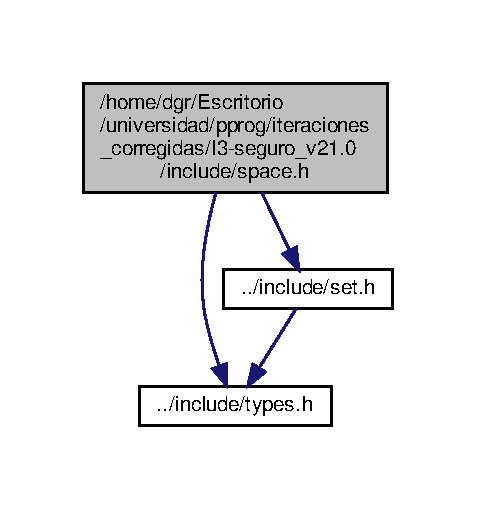
\includegraphics[width=236pt]{space_8h__incl}
\end{center}
\end{figure}
This graph shows which files directly or indirectly include this file\+:\nopagebreak
\begin{figure}[H]
\begin{center}
\leavevmode
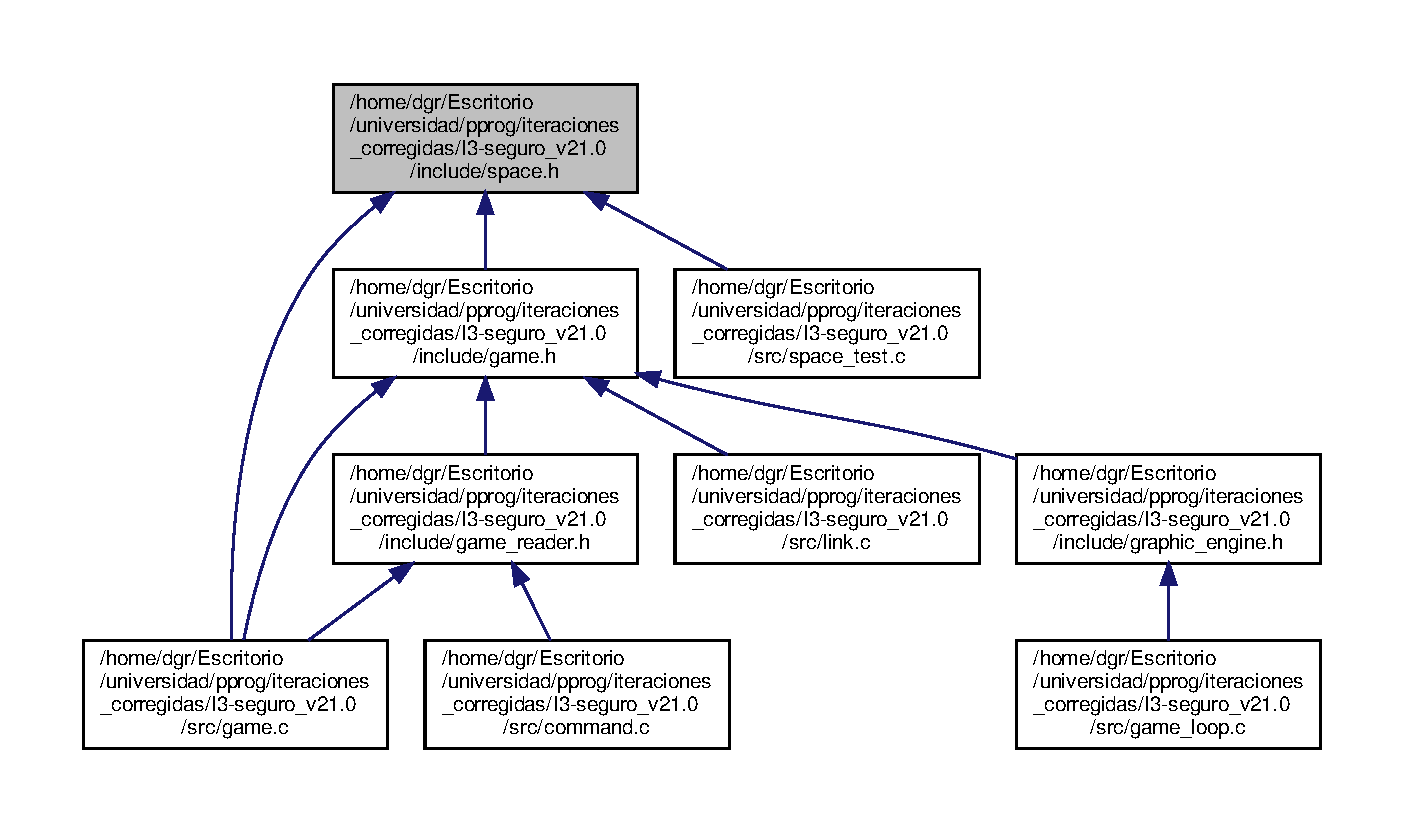
\includegraphics[width=350pt]{space_8h__dep__incl}
\end{center}
\end{figure}
\subsection*{Macros}
\begin{DoxyCompactItemize}
\item 
\#define \hyperlink{space_8h_a5f54fd55f983a2e33ce076cd9f587e82}{M\+A\+X\+\_\+\+S\+P\+A\+C\+ES}~100
\begin{DoxyCompactList}\small\item\em A macro that stores the maximum number of spaces. \end{DoxyCompactList}\item 
\#define \hyperlink{space_8h_a088cbe7c6f78264d46c2624194c5c680}{F\+I\+R\+S\+T\+\_\+\+S\+P\+A\+CE}~1
\begin{DoxyCompactList}\small\item\em A macro that stores the id of the first id. \end{DoxyCompactList}\item 
\#define \hyperlink{space_8h_a9c6419e7f541d4daf14f5ccd56e03f17}{N\+U\+M\+\_\+\+S\+T\+R\+I\+N\+GS}~3
\begin{DoxyCompactList}\small\item\em the number of strings of a gdesc \end{DoxyCompactList}\item 
\#define \hyperlink{space_8h_a4f7414c5a72de21b6b45d462410dfc97}{N\+U\+M\+\_\+\+C\+H\+A\+R\+A\+C\+TS}~7
\begin{DoxyCompactList}\small\item\em A macro that stores the number of chars per string of a gdesc. \end{DoxyCompactList}\end{DoxyCompactItemize}
\subsection*{Typedefs}
\begin{DoxyCompactItemize}
\item 
typedef struct \hyperlink{struct__Space}{\+\_\+\+Space} \hyperlink{space_8h_a67533ffc2b70463baecc38fb0629bbfc}{Space}
\begin{DoxyCompactList}\small\item\em A type definition for a space. \end{DoxyCompactList}\end{DoxyCompactItemize}
\subsection*{Functions}
\begin{DoxyCompactItemize}
\item 
\hyperlink{space_8h_a67533ffc2b70463baecc38fb0629bbfc}{Space} $\ast$ \hyperlink{space_8h_a162866fcea156b800fd546d0ffd271c9}{space\+\_\+create} (\hyperlink{types_8h_a845e604fb28f7e3d97549da3448149d3}{Id} id)
\begin{DoxyCompactList}\small\item\em Create the space. \end{DoxyCompactList}\item 
\hyperlink{types_8h_a32c27cc471df37f4fc818d65de0a56c4}{S\+T\+A\+T\+US} \hyperlink{space_8h_a5c70c70398923693ddbe4dfac8d72a0d}{space\+\_\+destroy} (\hyperlink{space_8h_a67533ffc2b70463baecc38fb0629bbfc}{Space} $\ast$space)
\begin{DoxyCompactList}\small\item\em free a space \end{DoxyCompactList}\item 
\hyperlink{types_8h_a845e604fb28f7e3d97549da3448149d3}{Id} \hyperlink{space_8h_ac8ddfd0d8692fd852ee49698c446cb50}{space\+\_\+get\+\_\+id} (\hyperlink{space_8h_a67533ffc2b70463baecc38fb0629bbfc}{Space} $\ast$space)
\begin{DoxyCompactList}\small\item\em get the id of the space \end{DoxyCompactList}\item 
\hyperlink{types_8h_a32c27cc471df37f4fc818d65de0a56c4}{S\+T\+A\+T\+US} \hyperlink{space_8h_aab5b468f9822ab78dbe16d1321870d93}{space\+\_\+set\+\_\+name} (\hyperlink{space_8h_a67533ffc2b70463baecc38fb0629bbfc}{Space} $\ast$space, char $\ast$name)
\begin{DoxyCompactList}\small\item\em name the space \end{DoxyCompactList}\item 
const char $\ast$ \hyperlink{space_8h_a310c540cd6e11073f7328add1f927001}{space\+\_\+get\+\_\+name} (\hyperlink{space_8h_a67533ffc2b70463baecc38fb0629bbfc}{Space} $\ast$space)
\begin{DoxyCompactList}\small\item\em get the name of the space \end{DoxyCompactList}\item 
\hyperlink{types_8h_a32c27cc471df37f4fc818d65de0a56c4}{S\+T\+A\+T\+US} \hyperlink{space_8h_a9e6e3e3bac4996ac6b8bd555e52bfb26}{space\+\_\+set\+\_\+north} (\hyperlink{space_8h_a67533ffc2b70463baecc38fb0629bbfc}{Space} $\ast$space, \hyperlink{types_8h_a845e604fb28f7e3d97549da3448149d3}{Id} id)
\begin{DoxyCompactList}\small\item\em set the north \end{DoxyCompactList}\item 
\hyperlink{types_8h_a845e604fb28f7e3d97549da3448149d3}{Id} \hyperlink{space_8h_ad331fba774897900f615d9d2e8d81a90}{space\+\_\+get\+\_\+north} (\hyperlink{space_8h_a67533ffc2b70463baecc38fb0629bbfc}{Space} $\ast$space)
\begin{DoxyCompactList}\small\item\em get the north of the space \end{DoxyCompactList}\item 
\hyperlink{types_8h_a32c27cc471df37f4fc818d65de0a56c4}{S\+T\+A\+T\+US} \hyperlink{space_8h_a422ab9f220b4c471c44256a27377de1a}{space\+\_\+set\+\_\+south} (\hyperlink{space_8h_a67533ffc2b70463baecc38fb0629bbfc}{Space} $\ast$space, \hyperlink{types_8h_a845e604fb28f7e3d97549da3448149d3}{Id} id)
\begin{DoxyCompactList}\small\item\em set the south \end{DoxyCompactList}\item 
\hyperlink{types_8h_a845e604fb28f7e3d97549da3448149d3}{Id} \hyperlink{space_8h_a9b86e1335c423eaad832e50d4c12cf1f}{space\+\_\+get\+\_\+south} (\hyperlink{space_8h_a67533ffc2b70463baecc38fb0629bbfc}{Space} $\ast$space)
\begin{DoxyCompactList}\small\item\em get the south of the space \end{DoxyCompactList}\item 
\hyperlink{types_8h_a32c27cc471df37f4fc818d65de0a56c4}{S\+T\+A\+T\+US} \hyperlink{space_8h_a860a8f3e0227955ad56d1a12f0bdc44a}{space\+\_\+set\+\_\+east} (\hyperlink{space_8h_a67533ffc2b70463baecc38fb0629bbfc}{Space} $\ast$space, \hyperlink{types_8h_a845e604fb28f7e3d97549da3448149d3}{Id} id)
\begin{DoxyCompactList}\small\item\em set the east \end{DoxyCompactList}\item 
\hyperlink{types_8h_a845e604fb28f7e3d97549da3448149d3}{Id} \hyperlink{space_8h_a978a22b77f74bb2dab68a00571abbe0b}{space\+\_\+get\+\_\+east} (\hyperlink{space_8h_a67533ffc2b70463baecc38fb0629bbfc}{Space} $\ast$space)
\begin{DoxyCompactList}\small\item\em get the east of the space \end{DoxyCompactList}\item 
\hyperlink{types_8h_a32c27cc471df37f4fc818d65de0a56c4}{S\+T\+A\+T\+US} \hyperlink{space_8h_ad44b14cb38902cf31fa1f341beaab0db}{space\+\_\+set\+\_\+west} (\hyperlink{space_8h_a67533ffc2b70463baecc38fb0629bbfc}{Space} $\ast$space, \hyperlink{types_8h_a845e604fb28f7e3d97549da3448149d3}{Id} id)
\begin{DoxyCompactList}\small\item\em set the west \end{DoxyCompactList}\item 
\hyperlink{types_8h_a845e604fb28f7e3d97549da3448149d3}{Id} \hyperlink{space_8h_af495ebfd5d13eba1a48cebd10992a17f}{space\+\_\+get\+\_\+west} (\hyperlink{space_8h_a67533ffc2b70463baecc38fb0629bbfc}{Space} $\ast$space)
\begin{DoxyCompactList}\small\item\em get the west of the space \end{DoxyCompactList}\item 
\hyperlink{types_8h_a32c27cc471df37f4fc818d65de0a56c4}{S\+T\+A\+T\+US} \hyperlink{space_8h_ae5b9fef52456ffccffbd73f882a56d23}{space\+\_\+set\+\_\+down} (\hyperlink{space_8h_a67533ffc2b70463baecc38fb0629bbfc}{Space} $\ast$space, \hyperlink{types_8h_a845e604fb28f7e3d97549da3448149d3}{Id} id)
\begin{DoxyCompactList}\small\item\em set the down \end{DoxyCompactList}\item 
\hyperlink{types_8h_a845e604fb28f7e3d97549da3448149d3}{Id} \hyperlink{space_8h_ab269eab72b9ea7254044b34b1c177602}{space\+\_\+get\+\_\+down} (\hyperlink{space_8h_a67533ffc2b70463baecc38fb0629bbfc}{Space} $\ast$space)
\begin{DoxyCompactList}\small\item\em get the down of the space \end{DoxyCompactList}\item 
\hyperlink{types_8h_a32c27cc471df37f4fc818d65de0a56c4}{S\+T\+A\+T\+US} \hyperlink{space_8h_aa2707bdca8fd356ed8d15fd48e820a4f}{space\+\_\+set\+\_\+up} (\hyperlink{space_8h_a67533ffc2b70463baecc38fb0629bbfc}{Space} $\ast$space, \hyperlink{types_8h_a845e604fb28f7e3d97549da3448149d3}{Id} id)
\begin{DoxyCompactList}\small\item\em set the up \end{DoxyCompactList}\item 
\hyperlink{types_8h_a845e604fb28f7e3d97549da3448149d3}{Id} \hyperlink{space_8h_a174a988b899d5a0db889a31b70763c9c}{space\+\_\+get\+\_\+up} (\hyperlink{space_8h_a67533ffc2b70463baecc38fb0629bbfc}{Space} $\ast$space)
\begin{DoxyCompactList}\small\item\em get the up of the space \end{DoxyCompactList}\item 
\hyperlink{types_8h_a32c27cc471df37f4fc818d65de0a56c4}{S\+T\+A\+T\+US} \hyperlink{space_8h_a3c7f18ed5814b6014f994a6bd268ed93}{space\+\_\+add\+\_\+object} (\hyperlink{space_8h_a67533ffc2b70463baecc38fb0629bbfc}{Space} $\ast$space, \hyperlink{types_8h_a845e604fb28f7e3d97549da3448149d3}{Id} object)
\begin{DoxyCompactList}\small\item\em set the object \end{DoxyCompactList}\item 
\hyperlink{set_8h_a6d3b7f7c92cbb4577ef3ef7ddbf93161}{Set} $\ast$ \hyperlink{space_8h_afc0e3f36d3bdf0105c5d25c256c9cfbd}{space\+\_\+get\+\_\+objects} (\hyperlink{space_8h_a67533ffc2b70463baecc38fb0629bbfc}{Space} $\ast$space)
\begin{DoxyCompactList}\small\item\em get the object of this space \end{DoxyCompactList}\item 
\hyperlink{types_8h_a32c27cc471df37f4fc818d65de0a56c4}{S\+T\+A\+T\+US} \hyperlink{space_8h_a18eca058da6cdf20ae5eda9d122d992e}{space\+\_\+print} (\hyperlink{space_8h_a67533ffc2b70463baecc38fb0629bbfc}{Space} $\ast$space)
\begin{DoxyCompactList}\small\item\em printf the space on the screen \end{DoxyCompactList}\item 
char \hyperlink{space_8h_a83a81b50900122edbcad7de9ad7a12ab}{space\+\_\+get\+\_\+gdesc\+\_\+at} (\hyperlink{space_8h_a67533ffc2b70463baecc38fb0629bbfc}{Space} $\ast$space, int position1, int position2)
\begin{DoxyCompactList}\small\item\em get an especific element of the array of string \end{DoxyCompactList}\item 
\hyperlink{types_8h_a32c27cc471df37f4fc818d65de0a56c4}{S\+T\+A\+T\+US} \hyperlink{space_8h_aa0946c480abf293fe9a7bb208037da5c}{space\+\_\+set\+\_\+gdesc\+\_\+at} (\hyperlink{space_8h_a67533ffc2b70463baecc38fb0629bbfc}{Space} $\ast$space, int position1, int position2, char element)
\begin{DoxyCompactList}\small\item\em get an especific element of the array of string \end{DoxyCompactList}\item 
\hyperlink{types_8h_a3e5b8192e7d9ffaf3542f1210aec18dd}{B\+O\+OL} \hyperlink{space_8h_aa7e388700d59402e9222d2f19af46ad1}{space\+\_\+is\+\_\+object} (\hyperlink{space_8h_a67533ffc2b70463baecc38fb0629bbfc}{Space} $\ast$space, \hyperlink{types_8h_a845e604fb28f7e3d97549da3448149d3}{Id} object)
\begin{DoxyCompactList}\small\item\em used to know if an object is in a space or not \end{DoxyCompactList}\item 
\hyperlink{types_8h_a32c27cc471df37f4fc818d65de0a56c4}{S\+T\+A\+T\+US} \hyperlink{space_8h_afa6c76219b25bc0d25827cd27f8464fe}{space\+\_\+dell\+\_\+object} (\hyperlink{space_8h_a67533ffc2b70463baecc38fb0629bbfc}{Space} $\ast$space, \hyperlink{types_8h_a845e604fb28f7e3d97549da3448149d3}{Id} object)
\begin{DoxyCompactList}\small\item\em used to dell an object in an space \end{DoxyCompactList}\item 
int \hyperlink{space_8h_a1f6b218608de895d9b82e53e992b3175}{space\+\_\+get\+\_\+num} (\hyperlink{space_8h_a67533ffc2b70463baecc38fb0629bbfc}{Space} $\ast$space)
\begin{DoxyCompactList}\small\item\em used to know the amount of obects in the space \end{DoxyCompactList}\item 
const char $\ast$ \hyperlink{space_8h_ae4e07e1125da9f7096eb5eba116cea7e}{space\+\_\+get\+\_\+description1} (\hyperlink{space_8h_a67533ffc2b70463baecc38fb0629bbfc}{Space} $\ast$space)
\begin{DoxyCompactList}\small\item\em used to know the description of an space no matter if the space is lit or not \end{DoxyCompactList}\item 
const char $\ast$ \hyperlink{space_8h_a209cf4c49f15e49cdd77863ca5a415e3}{space\+\_\+get\+\_\+description2} (\hyperlink{space_8h_a67533ffc2b70463baecc38fb0629bbfc}{Space} $\ast$space)
\begin{DoxyCompactList}\small\item\em used to know the description of an space if the space is lit \end{DoxyCompactList}\item 
\hyperlink{types_8h_a32c27cc471df37f4fc818d65de0a56c4}{S\+T\+A\+T\+US} \hyperlink{space_8h_a2800febfcfd5d519c2f937d85d69c2d4}{space\+\_\+set\+\_\+description1} (\hyperlink{space_8h_a67533ffc2b70463baecc38fb0629bbfc}{Space} $\ast$space, char $\ast$description)
\begin{DoxyCompactList}\small\item\em used to set the description which you can see no matter if the space is lit or not \end{DoxyCompactList}\item 
\hyperlink{types_8h_a32c27cc471df37f4fc818d65de0a56c4}{S\+T\+A\+T\+US} \hyperlink{space_8h_ad206f89335e1ca729bef9909c654f153}{space\+\_\+set\+\_\+description2} (\hyperlink{space_8h_a67533ffc2b70463baecc38fb0629bbfc}{Space} $\ast$space, char $\ast$description)
\begin{DoxyCompactList}\small\item\em used to set the description which you can see no matter if the space is lit \end{DoxyCompactList}\item 
\hyperlink{types_8h_a3e5b8192e7d9ffaf3542f1210aec18dd}{B\+O\+OL} \hyperlink{space_8h_a2dea60f1cac073e20256df7a47a0d07d}{space\+\_\+is\+\_\+iluminated} (\hyperlink{space_8h_a67533ffc2b70463baecc38fb0629bbfc}{Space} $\ast$space)
\begin{DoxyCompactList}\small\item\em used to see if an space is iluminated or not \end{DoxyCompactList}\item 
\hyperlink{types_8h_a32c27cc471df37f4fc818d65de0a56c4}{S\+T\+A\+T\+US} \hyperlink{space_8h_af92c62ffae0b7dc4dc703210e032dc48}{space\+\_\+set\+\_\+ilumination} (\hyperlink{space_8h_a67533ffc2b70463baecc38fb0629bbfc}{Space} $\ast$space, \hyperlink{types_8h_a3e5b8192e7d9ffaf3542f1210aec18dd}{B\+O\+OL} bool)
\begin{DoxyCompactList}\small\item\em used to set the ilumination of an space \end{DoxyCompactList}\end{DoxyCompactItemize}


\subsection{Detailed Description}
It defines a space. 

\begin{DoxyAuthor}{Author}
Profesores P\+P\+R\+OG, David Teófilo Garitagoitia Romero, José Manuel García Giráldez 
\end{DoxyAuthor}
\begin{DoxyVersion}{Version}
1.\+0 
\end{DoxyVersion}
\begin{DoxyDate}{Date}
13-\/01-\/2015 
\end{DoxyDate}
\begin{DoxyCopyright}{Copyright}
G\+NU Public License 
\end{DoxyCopyright}


\subsection{Macro Definition Documentation}
\mbox{\Hypertarget{space_8h_a088cbe7c6f78264d46c2624194c5c680}\label{space_8h_a088cbe7c6f78264d46c2624194c5c680}} 
\index{space.\+h@{space.\+h}!F\+I\+R\+S\+T\+\_\+\+S\+P\+A\+CE@{F\+I\+R\+S\+T\+\_\+\+S\+P\+A\+CE}}
\index{F\+I\+R\+S\+T\+\_\+\+S\+P\+A\+CE@{F\+I\+R\+S\+T\+\_\+\+S\+P\+A\+CE}!space.\+h@{space.\+h}}
\subsubsection{\texorpdfstring{F\+I\+R\+S\+T\+\_\+\+S\+P\+A\+CE}{FIRST\_SPACE}}
{\footnotesize\ttfamily \#define F\+I\+R\+S\+T\+\_\+\+S\+P\+A\+CE~1}



A macro that stores the id of the first id. 

Details. \mbox{\Hypertarget{space_8h_a5f54fd55f983a2e33ce076cd9f587e82}\label{space_8h_a5f54fd55f983a2e33ce076cd9f587e82}} 
\index{space.\+h@{space.\+h}!M\+A\+X\+\_\+\+S\+P\+A\+C\+ES@{M\+A\+X\+\_\+\+S\+P\+A\+C\+ES}}
\index{M\+A\+X\+\_\+\+S\+P\+A\+C\+ES@{M\+A\+X\+\_\+\+S\+P\+A\+C\+ES}!space.\+h@{space.\+h}}
\subsubsection{\texorpdfstring{M\+A\+X\+\_\+\+S\+P\+A\+C\+ES}{MAX\_SPACES}}
{\footnotesize\ttfamily \#define M\+A\+X\+\_\+\+S\+P\+A\+C\+ES~100}



A macro that stores the maximum number of spaces. 

Details. \mbox{\Hypertarget{space_8h_a4f7414c5a72de21b6b45d462410dfc97}\label{space_8h_a4f7414c5a72de21b6b45d462410dfc97}} 
\index{space.\+h@{space.\+h}!N\+U\+M\+\_\+\+C\+H\+A\+R\+A\+C\+TS@{N\+U\+M\+\_\+\+C\+H\+A\+R\+A\+C\+TS}}
\index{N\+U\+M\+\_\+\+C\+H\+A\+R\+A\+C\+TS@{N\+U\+M\+\_\+\+C\+H\+A\+R\+A\+C\+TS}!space.\+h@{space.\+h}}
\subsubsection{\texorpdfstring{N\+U\+M\+\_\+\+C\+H\+A\+R\+A\+C\+TS}{NUM\_CHARACTS}}
{\footnotesize\ttfamily \#define N\+U\+M\+\_\+\+C\+H\+A\+R\+A\+C\+TS~7}



A macro that stores the number of chars per string of a gdesc. 

Details. \mbox{\Hypertarget{space_8h_a9c6419e7f541d4daf14f5ccd56e03f17}\label{space_8h_a9c6419e7f541d4daf14f5ccd56e03f17}} 
\index{space.\+h@{space.\+h}!N\+U\+M\+\_\+\+S\+T\+R\+I\+N\+GS@{N\+U\+M\+\_\+\+S\+T\+R\+I\+N\+GS}}
\index{N\+U\+M\+\_\+\+S\+T\+R\+I\+N\+GS@{N\+U\+M\+\_\+\+S\+T\+R\+I\+N\+GS}!space.\+h@{space.\+h}}
\subsubsection{\texorpdfstring{N\+U\+M\+\_\+\+S\+T\+R\+I\+N\+GS}{NUM\_STRINGS}}
{\footnotesize\ttfamily \#define N\+U\+M\+\_\+\+S\+T\+R\+I\+N\+GS~3}



the number of strings of a gdesc 

Details. 

\subsection{Typedef Documentation}
\mbox{\Hypertarget{space_8h_a67533ffc2b70463baecc38fb0629bbfc}\label{space_8h_a67533ffc2b70463baecc38fb0629bbfc}} 
\index{space.\+h@{space.\+h}!Space@{Space}}
\index{Space@{Space}!space.\+h@{space.\+h}}
\subsubsection{\texorpdfstring{Space}{Space}}
{\footnotesize\ttfamily typedef struct \hyperlink{struct__Space}{\+\_\+\+Space} \hyperlink{space_8h_a67533ffc2b70463baecc38fb0629bbfc}{Space}}



A type definition for a space. 

Details. 

\subsection{Function Documentation}
\mbox{\Hypertarget{space_8h_a3c7f18ed5814b6014f994a6bd268ed93}\label{space_8h_a3c7f18ed5814b6014f994a6bd268ed93}} 
\index{space.\+h@{space.\+h}!space\+\_\+add\+\_\+object@{space\+\_\+add\+\_\+object}}
\index{space\+\_\+add\+\_\+object@{space\+\_\+add\+\_\+object}!space.\+h@{space.\+h}}
\subsubsection{\texorpdfstring{space\+\_\+add\+\_\+object()}{space\_add\_object()}}
{\footnotesize\ttfamily \hyperlink{types_8h_a32c27cc471df37f4fc818d65de0a56c4}{S\+T\+A\+T\+US} space\+\_\+add\+\_\+object (\begin{DoxyParamCaption}\item[{\hyperlink{space_8h_a67533ffc2b70463baecc38fb0629bbfc}{Space} $\ast$}]{space,  }\item[{\hyperlink{types_8h_a845e604fb28f7e3d97549da3448149d3}{Id}}]{object }\end{DoxyParamCaption})}



set the object 

\begin{DoxyDate}{Date}
13-\/01-\/2015 
\end{DoxyDate}
\begin{DoxyAuthor}{Author}
\+: Instructors of P\+P\+R\+OG
\end{DoxyAuthor}

\begin{DoxyParams}{Parameters}
{\em space} & one space that has been created before \\
\hline
{\em object} & the id that the object will have \\
\hline
\end{DoxyParams}
\begin{DoxyReturn}{Returns}
E\+R\+R\+OR if there is an error, otherwise return OK 
\end{DoxyReturn}
\mbox{\Hypertarget{space_8h_a162866fcea156b800fd546d0ffd271c9}\label{space_8h_a162866fcea156b800fd546d0ffd271c9}} 
\index{space.\+h@{space.\+h}!space\+\_\+create@{space\+\_\+create}}
\index{space\+\_\+create@{space\+\_\+create}!space.\+h@{space.\+h}}
\subsubsection{\texorpdfstring{space\+\_\+create()}{space\_create()}}
{\footnotesize\ttfamily \hyperlink{space_8h_a67533ffc2b70463baecc38fb0629bbfc}{Space}$\ast$ space\+\_\+create (\begin{DoxyParamCaption}\item[{\hyperlink{types_8h_a845e604fb28f7e3d97549da3448149d3}{Id}}]{id }\end{DoxyParamCaption})}



Create the space. 

space\+\_\+create Create a space with a specific Id

\begin{DoxyDate}{Date}
13-\/01-\/2015 
\end{DoxyDate}
\begin{DoxyAuthor}{Author}
\+: Instructors of P\+P\+R\+OG
\end{DoxyAuthor}

\begin{DoxyParams}{Parameters}
{\em id} & the id of the new space \\
\hline
\end{DoxyParams}
\begin{DoxyReturn}{Returns}
the new space that has been created 
\end{DoxyReturn}
\mbox{\Hypertarget{space_8h_afa6c76219b25bc0d25827cd27f8464fe}\label{space_8h_afa6c76219b25bc0d25827cd27f8464fe}} 
\index{space.\+h@{space.\+h}!space\+\_\+dell\+\_\+object@{space\+\_\+dell\+\_\+object}}
\index{space\+\_\+dell\+\_\+object@{space\+\_\+dell\+\_\+object}!space.\+h@{space.\+h}}
\subsubsection{\texorpdfstring{space\+\_\+dell\+\_\+object()}{space\_dell\_object()}}
{\footnotesize\ttfamily \hyperlink{types_8h_a32c27cc471df37f4fc818d65de0a56c4}{S\+T\+A\+T\+US} space\+\_\+dell\+\_\+object (\begin{DoxyParamCaption}\item[{\hyperlink{space_8h_a67533ffc2b70463baecc38fb0629bbfc}{Space} $\ast$}]{space,  }\item[{\hyperlink{types_8h_a845e604fb28f7e3d97549da3448149d3}{Id}}]{object }\end{DoxyParamCaption})}



used to dell an object in an space 

\begin{DoxyDate}{Date}
20-\/02-\/2020 
\end{DoxyDate}
\begin{DoxyAuthor}{Author}
\+: David Teófilo Garitagoitia Romero
\end{DoxyAuthor}

\begin{DoxyParams}{Parameters}
{\em space} & one space that has been created before \\
\hline
{\em object} & the object that you want to remove \\
\hline
\end{DoxyParams}
\begin{DoxyReturn}{Returns}
E\+R\+R\+OR if there is an error, otherwise return OK 
\end{DoxyReturn}
\mbox{\Hypertarget{space_8h_a5c70c70398923693ddbe4dfac8d72a0d}\label{space_8h_a5c70c70398923693ddbe4dfac8d72a0d}} 
\index{space.\+h@{space.\+h}!space\+\_\+destroy@{space\+\_\+destroy}}
\index{space\+\_\+destroy@{space\+\_\+destroy}!space.\+h@{space.\+h}}
\subsubsection{\texorpdfstring{space\+\_\+destroy()}{space\_destroy()}}
{\footnotesize\ttfamily \hyperlink{types_8h_a32c27cc471df37f4fc818d65de0a56c4}{S\+T\+A\+T\+US} space\+\_\+destroy (\begin{DoxyParamCaption}\item[{\hyperlink{space_8h_a67533ffc2b70463baecc38fb0629bbfc}{Space} $\ast$}]{space }\end{DoxyParamCaption})}



free a space 

space\+\_\+destroy free a especific space

\begin{DoxyDate}{Date}
13-\/01-\/2015 
\end{DoxyDate}
\begin{DoxyAuthor}{Author}
\+: Instructors of P\+P\+R\+OG
\end{DoxyAuthor}

\begin{DoxyParams}{Parameters}
{\em space} & one space that has been created before \\
\hline
\end{DoxyParams}
\begin{DoxyReturn}{Returns}
E\+R\+R\+OR if there is an error, otherwise return OK 
\end{DoxyReturn}
\mbox{\Hypertarget{space_8h_ae4e07e1125da9f7096eb5eba116cea7e}\label{space_8h_ae4e07e1125da9f7096eb5eba116cea7e}} 
\index{space.\+h@{space.\+h}!space\+\_\+get\+\_\+description1@{space\+\_\+get\+\_\+description1}}
\index{space\+\_\+get\+\_\+description1@{space\+\_\+get\+\_\+description1}!space.\+h@{space.\+h}}
\subsubsection{\texorpdfstring{space\+\_\+get\+\_\+description1()}{space\_get\_description1()}}
{\footnotesize\ttfamily const char$\ast$ space\+\_\+get\+\_\+description1 (\begin{DoxyParamCaption}\item[{\hyperlink{space_8h_a67533ffc2b70463baecc38fb0629bbfc}{Space} $\ast$}]{space }\end{DoxyParamCaption})}



used to know the description of an space no matter if the space is lit or not 

\begin{DoxyDate}{Date}
10-\/03-\/2020 
\end{DoxyDate}
\begin{DoxyAuthor}{Author}
\+: David Teófilo Garitagoitia Romero
\end{DoxyAuthor}

\begin{DoxyParams}{Parameters}
{\em space} & one space that has been created before \\
\hline
\end{DoxyParams}
\begin{DoxyReturn}{Returns}
the description 
\end{DoxyReturn}
\mbox{\Hypertarget{space_8h_a209cf4c49f15e49cdd77863ca5a415e3}\label{space_8h_a209cf4c49f15e49cdd77863ca5a415e3}} 
\index{space.\+h@{space.\+h}!space\+\_\+get\+\_\+description2@{space\+\_\+get\+\_\+description2}}
\index{space\+\_\+get\+\_\+description2@{space\+\_\+get\+\_\+description2}!space.\+h@{space.\+h}}
\subsubsection{\texorpdfstring{space\+\_\+get\+\_\+description2()}{space\_get\_description2()}}
{\footnotesize\ttfamily const char$\ast$ space\+\_\+get\+\_\+description2 (\begin{DoxyParamCaption}\item[{\hyperlink{space_8h_a67533ffc2b70463baecc38fb0629bbfc}{Space} $\ast$}]{space }\end{DoxyParamCaption})}



used to know the description of an space if the space is lit 

\begin{DoxyDate}{Date}
10-\/04-\/2020 
\end{DoxyDate}
\begin{DoxyAuthor}{Author}
\+: David Teófilo Garitagoitia Romero
\end{DoxyAuthor}

\begin{DoxyParams}{Parameters}
{\em space} & one space that has been created before \\
\hline
\end{DoxyParams}
\begin{DoxyReturn}{Returns}
the most exact description 
\end{DoxyReturn}
\mbox{\Hypertarget{space_8h_ab269eab72b9ea7254044b34b1c177602}\label{space_8h_ab269eab72b9ea7254044b34b1c177602}} 
\index{space.\+h@{space.\+h}!space\+\_\+get\+\_\+down@{space\+\_\+get\+\_\+down}}
\index{space\+\_\+get\+\_\+down@{space\+\_\+get\+\_\+down}!space.\+h@{space.\+h}}
\subsubsection{\texorpdfstring{space\+\_\+get\+\_\+down()}{space\_get\_down()}}
{\footnotesize\ttfamily \hyperlink{types_8h_a845e604fb28f7e3d97549da3448149d3}{Id} space\+\_\+get\+\_\+down (\begin{DoxyParamCaption}\item[{\hyperlink{space_8h_a67533ffc2b70463baecc38fb0629bbfc}{Space} $\ast$}]{space }\end{DoxyParamCaption})}



get the down of the space 

\begin{DoxyDate}{Date}
11-\/04-\/2020 
\end{DoxyDate}
\begin{DoxyAuthor}{Author}
\+: David Teófilo Garitagoitia Romero
\end{DoxyAuthor}

\begin{DoxyParams}{Parameters}
{\em space} & one space that has been created before \\
\hline
\end{DoxyParams}
\begin{DoxyReturn}{Returns}
sapace-\/$>$down the down of the space we enter 
\end{DoxyReturn}
\mbox{\Hypertarget{space_8h_a978a22b77f74bb2dab68a00571abbe0b}\label{space_8h_a978a22b77f74bb2dab68a00571abbe0b}} 
\index{space.\+h@{space.\+h}!space\+\_\+get\+\_\+east@{space\+\_\+get\+\_\+east}}
\index{space\+\_\+get\+\_\+east@{space\+\_\+get\+\_\+east}!space.\+h@{space.\+h}}
\subsubsection{\texorpdfstring{space\+\_\+get\+\_\+east()}{space\_get\_east()}}
{\footnotesize\ttfamily \hyperlink{types_8h_a845e604fb28f7e3d97549da3448149d3}{Id} space\+\_\+get\+\_\+east (\begin{DoxyParamCaption}\item[{\hyperlink{space_8h_a67533ffc2b70463baecc38fb0629bbfc}{Space} $\ast$}]{space }\end{DoxyParamCaption})}



get the east of the space 

\begin{DoxyDate}{Date}
13-\/01-\/2015 
\end{DoxyDate}
\begin{DoxyAuthor}{Author}
\+: Instructors of P\+P\+R\+OG
\end{DoxyAuthor}

\begin{DoxyParams}{Parameters}
{\em space} & one space that has been created before \\
\hline
\end{DoxyParams}
\begin{DoxyReturn}{Returns}
sapace-\/$>$east the east of the space we enter 
\end{DoxyReturn}
\mbox{\Hypertarget{space_8h_a83a81b50900122edbcad7de9ad7a12ab}\label{space_8h_a83a81b50900122edbcad7de9ad7a12ab}} 
\index{space.\+h@{space.\+h}!space\+\_\+get\+\_\+gdesc\+\_\+at@{space\+\_\+get\+\_\+gdesc\+\_\+at}}
\index{space\+\_\+get\+\_\+gdesc\+\_\+at@{space\+\_\+get\+\_\+gdesc\+\_\+at}!space.\+h@{space.\+h}}
\subsubsection{\texorpdfstring{space\+\_\+get\+\_\+gdesc\+\_\+at()}{space\_get\_gdesc\_at()}}
{\footnotesize\ttfamily char space\+\_\+get\+\_\+gdesc\+\_\+at (\begin{DoxyParamCaption}\item[{\hyperlink{space_8h_a67533ffc2b70463baecc38fb0629bbfc}{Space} $\ast$}]{space,  }\item[{int}]{position1,  }\item[{int}]{position2 }\end{DoxyParamCaption})}



get an especific element of the array of string 

\begin{DoxyDate}{Date}
13-\/01-\/2015 
\end{DoxyDate}
\begin{DoxyAuthor}{Author}
\+: José Manuel García Giráldez
\end{DoxyAuthor}

\begin{DoxyParams}{Parameters}
{\em space} & one space that has been created before \\
\hline
{\em position1} & select the string we want \\
\hline
{\em position2} & select the element of the string we want \\
\hline
\end{DoxyParams}
\begin{DoxyReturn}{Returns}
the element we search for 
\end{DoxyReturn}
\mbox{\Hypertarget{space_8h_ac8ddfd0d8692fd852ee49698c446cb50}\label{space_8h_ac8ddfd0d8692fd852ee49698c446cb50}} 
\index{space.\+h@{space.\+h}!space\+\_\+get\+\_\+id@{space\+\_\+get\+\_\+id}}
\index{space\+\_\+get\+\_\+id@{space\+\_\+get\+\_\+id}!space.\+h@{space.\+h}}
\subsubsection{\texorpdfstring{space\+\_\+get\+\_\+id()}{space\_get\_id()}}
{\footnotesize\ttfamily \hyperlink{types_8h_a845e604fb28f7e3d97549da3448149d3}{Id} space\+\_\+get\+\_\+id (\begin{DoxyParamCaption}\item[{\hyperlink{space_8h_a67533ffc2b70463baecc38fb0629bbfc}{Space} $\ast$}]{space }\end{DoxyParamCaption})}



get the id of the space 

\begin{DoxyDate}{Date}
13-\/01-\/2015 
\end{DoxyDate}
\begin{DoxyAuthor}{Author}
\+: Instructors of P\+P\+R\+OG
\end{DoxyAuthor}

\begin{DoxyParams}{Parameters}
{\em space} & one space that has been created before \\
\hline
\end{DoxyParams}
\begin{DoxyReturn}{Returns}
sapace-\/$>$id the id of the space we enter 
\end{DoxyReturn}
\mbox{\Hypertarget{space_8h_a310c540cd6e11073f7328add1f927001}\label{space_8h_a310c540cd6e11073f7328add1f927001}} 
\index{space.\+h@{space.\+h}!space\+\_\+get\+\_\+name@{space\+\_\+get\+\_\+name}}
\index{space\+\_\+get\+\_\+name@{space\+\_\+get\+\_\+name}!space.\+h@{space.\+h}}
\subsubsection{\texorpdfstring{space\+\_\+get\+\_\+name()}{space\_get\_name()}}
{\footnotesize\ttfamily const char$\ast$ space\+\_\+get\+\_\+name (\begin{DoxyParamCaption}\item[{\hyperlink{space_8h_a67533ffc2b70463baecc38fb0629bbfc}{Space} $\ast$}]{space }\end{DoxyParamCaption})}



get the name of the space 

\begin{DoxyDate}{Date}
13-\/01-\/2015 
\end{DoxyDate}
\begin{DoxyAuthor}{Author}
\+: Instructors of P\+P\+R\+OG
\end{DoxyAuthor}

\begin{DoxyParams}{Parameters}
{\em space} & one space that has been created before \\
\hline
\end{DoxyParams}
\begin{DoxyReturn}{Returns}
sapace-\/$>$name the name of the space we enter 
\end{DoxyReturn}
\mbox{\Hypertarget{space_8h_ad331fba774897900f615d9d2e8d81a90}\label{space_8h_ad331fba774897900f615d9d2e8d81a90}} 
\index{space.\+h@{space.\+h}!space\+\_\+get\+\_\+north@{space\+\_\+get\+\_\+north}}
\index{space\+\_\+get\+\_\+north@{space\+\_\+get\+\_\+north}!space.\+h@{space.\+h}}
\subsubsection{\texorpdfstring{space\+\_\+get\+\_\+north()}{space\_get\_north()}}
{\footnotesize\ttfamily \hyperlink{types_8h_a845e604fb28f7e3d97549da3448149d3}{Id} space\+\_\+get\+\_\+north (\begin{DoxyParamCaption}\item[{\hyperlink{space_8h_a67533ffc2b70463baecc38fb0629bbfc}{Space} $\ast$}]{space }\end{DoxyParamCaption})}



get the north of the space 

\begin{DoxyDate}{Date}
13-\/01-\/2015 
\end{DoxyDate}
\begin{DoxyAuthor}{Author}
\+: Instructors of P\+P\+R\+OG
\end{DoxyAuthor}

\begin{DoxyParams}{Parameters}
{\em space} & one space that has been created before \\
\hline
\end{DoxyParams}
\begin{DoxyReturn}{Returns}
sapace-\/$>$north the north of the space we enter 
\end{DoxyReturn}
\mbox{\Hypertarget{space_8h_a1f6b218608de895d9b82e53e992b3175}\label{space_8h_a1f6b218608de895d9b82e53e992b3175}} 
\index{space.\+h@{space.\+h}!space\+\_\+get\+\_\+num@{space\+\_\+get\+\_\+num}}
\index{space\+\_\+get\+\_\+num@{space\+\_\+get\+\_\+num}!space.\+h@{space.\+h}}
\subsubsection{\texorpdfstring{space\+\_\+get\+\_\+num()}{space\_get\_num()}}
{\footnotesize\ttfamily int space\+\_\+get\+\_\+num (\begin{DoxyParamCaption}\item[{\hyperlink{space_8h_a67533ffc2b70463baecc38fb0629bbfc}{Space} $\ast$}]{space }\end{DoxyParamCaption})}



used to know the amount of obects in the space 

\begin{DoxyDate}{Date}
2-\/03-\/2020 
\end{DoxyDate}
\begin{DoxyAuthor}{Author}
\+: David Teófilo Garitagoitia Romero
\end{DoxyAuthor}

\begin{DoxyParams}{Parameters}
{\em space} & one space that has been created before \\
\hline
\end{DoxyParams}
\begin{DoxyReturn}{Returns}
the amount of objects 
\end{DoxyReturn}
\mbox{\Hypertarget{space_8h_afc0e3f36d3bdf0105c5d25c256c9cfbd}\label{space_8h_afc0e3f36d3bdf0105c5d25c256c9cfbd}} 
\index{space.\+h@{space.\+h}!space\+\_\+get\+\_\+objects@{space\+\_\+get\+\_\+objects}}
\index{space\+\_\+get\+\_\+objects@{space\+\_\+get\+\_\+objects}!space.\+h@{space.\+h}}
\subsubsection{\texorpdfstring{space\+\_\+get\+\_\+objects()}{space\_get\_objects()}}
{\footnotesize\ttfamily \hyperlink{set_8h_a6d3b7f7c92cbb4577ef3ef7ddbf93161}{Set}$\ast$ space\+\_\+get\+\_\+objects (\begin{DoxyParamCaption}\item[{\hyperlink{space_8h_a67533ffc2b70463baecc38fb0629bbfc}{Space} $\ast$}]{space }\end{DoxyParamCaption})}



get the object of this space 

\begin{DoxyDate}{Date}
13-\/01-\/2015 
\end{DoxyDate}
\begin{DoxyAuthor}{Author}
\+: Instructors of P\+P\+R\+OG
\end{DoxyAuthor}

\begin{DoxyParams}{Parameters}
{\em space} & one space that has been created before \\
\hline
\end{DoxyParams}
\begin{DoxyReturn}{Returns}
sapace-\/$>$object the object int the space we enter 
\end{DoxyReturn}
\mbox{\Hypertarget{space_8h_a9b86e1335c423eaad832e50d4c12cf1f}\label{space_8h_a9b86e1335c423eaad832e50d4c12cf1f}} 
\index{space.\+h@{space.\+h}!space\+\_\+get\+\_\+south@{space\+\_\+get\+\_\+south}}
\index{space\+\_\+get\+\_\+south@{space\+\_\+get\+\_\+south}!space.\+h@{space.\+h}}
\subsubsection{\texorpdfstring{space\+\_\+get\+\_\+south()}{space\_get\_south()}}
{\footnotesize\ttfamily \hyperlink{types_8h_a845e604fb28f7e3d97549da3448149d3}{Id} space\+\_\+get\+\_\+south (\begin{DoxyParamCaption}\item[{\hyperlink{space_8h_a67533ffc2b70463baecc38fb0629bbfc}{Space} $\ast$}]{space }\end{DoxyParamCaption})}



get the south of the space 

\begin{DoxyDate}{Date}
13-\/01-\/2015 
\end{DoxyDate}
\begin{DoxyAuthor}{Author}
\+: Instructors of P\+P\+R\+OG
\end{DoxyAuthor}

\begin{DoxyParams}{Parameters}
{\em space} & one space that has been created before \\
\hline
\end{DoxyParams}
\begin{DoxyReturn}{Returns}
sapace-\/$>$south the south of the space we enter 
\end{DoxyReturn}
\mbox{\Hypertarget{space_8h_a174a988b899d5a0db889a31b70763c9c}\label{space_8h_a174a988b899d5a0db889a31b70763c9c}} 
\index{space.\+h@{space.\+h}!space\+\_\+get\+\_\+up@{space\+\_\+get\+\_\+up}}
\index{space\+\_\+get\+\_\+up@{space\+\_\+get\+\_\+up}!space.\+h@{space.\+h}}
\subsubsection{\texorpdfstring{space\+\_\+get\+\_\+up()}{space\_get\_up()}}
{\footnotesize\ttfamily \hyperlink{types_8h_a845e604fb28f7e3d97549da3448149d3}{Id} space\+\_\+get\+\_\+up (\begin{DoxyParamCaption}\item[{\hyperlink{space_8h_a67533ffc2b70463baecc38fb0629bbfc}{Space} $\ast$}]{space }\end{DoxyParamCaption})}



get the up of the space 

\begin{DoxyDate}{Date}
11-\/04-\/2020 
\end{DoxyDate}
\begin{DoxyAuthor}{Author}
\+: David Teófilo Garitagoitia Romero
\end{DoxyAuthor}

\begin{DoxyParams}{Parameters}
{\em space} & one space that has been created before \\
\hline
\end{DoxyParams}
\begin{DoxyReturn}{Returns}
sapace-\/$>$up the up of the space we enter 
\end{DoxyReturn}
\mbox{\Hypertarget{space_8h_af495ebfd5d13eba1a48cebd10992a17f}\label{space_8h_af495ebfd5d13eba1a48cebd10992a17f}} 
\index{space.\+h@{space.\+h}!space\+\_\+get\+\_\+west@{space\+\_\+get\+\_\+west}}
\index{space\+\_\+get\+\_\+west@{space\+\_\+get\+\_\+west}!space.\+h@{space.\+h}}
\subsubsection{\texorpdfstring{space\+\_\+get\+\_\+west()}{space\_get\_west()}}
{\footnotesize\ttfamily \hyperlink{types_8h_a845e604fb28f7e3d97549da3448149d3}{Id} space\+\_\+get\+\_\+west (\begin{DoxyParamCaption}\item[{\hyperlink{space_8h_a67533ffc2b70463baecc38fb0629bbfc}{Space} $\ast$}]{space }\end{DoxyParamCaption})}



get the west of the space 

\begin{DoxyDate}{Date}
13-\/01-\/2015 
\end{DoxyDate}
\begin{DoxyAuthor}{Author}
\+: Instructors of P\+P\+R\+OG
\end{DoxyAuthor}

\begin{DoxyParams}{Parameters}
{\em space} & one space that has been created before \\
\hline
\end{DoxyParams}
\begin{DoxyReturn}{Returns}
sapace-\/$>$west the west of the space we enter 
\end{DoxyReturn}
\mbox{\Hypertarget{space_8h_a2dea60f1cac073e20256df7a47a0d07d}\label{space_8h_a2dea60f1cac073e20256df7a47a0d07d}} 
\index{space.\+h@{space.\+h}!space\+\_\+is\+\_\+iluminated@{space\+\_\+is\+\_\+iluminated}}
\index{space\+\_\+is\+\_\+iluminated@{space\+\_\+is\+\_\+iluminated}!space.\+h@{space.\+h}}
\subsubsection{\texorpdfstring{space\+\_\+is\+\_\+iluminated()}{space\_is\_iluminated()}}
{\footnotesize\ttfamily \hyperlink{types_8h_a3e5b8192e7d9ffaf3542f1210aec18dd}{B\+O\+OL} space\+\_\+is\+\_\+iluminated (\begin{DoxyParamCaption}\item[{\hyperlink{space_8h_a67533ffc2b70463baecc38fb0629bbfc}{Space} $\ast$}]{space }\end{DoxyParamCaption})}



used to see if an space is iluminated or not 

\begin{DoxyDate}{Date}
20-\/04-\/2020 
\end{DoxyDate}
\begin{DoxyAuthor}{Author}
\+: David Teófilo Garitagoitia Romero
\end{DoxyAuthor}

\begin{DoxyParams}{Parameters}
{\em space} & one space that has been created before \\
\hline
\end{DoxyParams}
\begin{DoxyReturn}{Returns}
True if its iluminate, false otherwise 
\end{DoxyReturn}
\mbox{\Hypertarget{space_8h_aa7e388700d59402e9222d2f19af46ad1}\label{space_8h_aa7e388700d59402e9222d2f19af46ad1}} 
\index{space.\+h@{space.\+h}!space\+\_\+is\+\_\+object@{space\+\_\+is\+\_\+object}}
\index{space\+\_\+is\+\_\+object@{space\+\_\+is\+\_\+object}!space.\+h@{space.\+h}}
\subsubsection{\texorpdfstring{space\+\_\+is\+\_\+object()}{space\_is\_object()}}
{\footnotesize\ttfamily \hyperlink{types_8h_a3e5b8192e7d9ffaf3542f1210aec18dd}{B\+O\+OL} space\+\_\+is\+\_\+object (\begin{DoxyParamCaption}\item[{\hyperlink{space_8h_a67533ffc2b70463baecc38fb0629bbfc}{Space} $\ast$}]{space,  }\item[{\hyperlink{types_8h_a845e604fb28f7e3d97549da3448149d3}{Id}}]{object }\end{DoxyParamCaption})}



used to know if an object is in a space or not 

\begin{DoxyDate}{Date}
20-\/02-\/2020 
\end{DoxyDate}
\begin{DoxyAuthor}{Author}
\+: David Teófilo Garitagoitia Romero
\end{DoxyAuthor}

\begin{DoxyParams}{Parameters}
{\em space} & one space that has been created before \\
\hline
{\em object} & the object that you want to know if is in the space or not \\
\hline
\end{DoxyParams}
\begin{DoxyReturn}{Returns}
E\+R\+R\+OR if there is an error, otherwise return OK 
\end{DoxyReturn}
\mbox{\Hypertarget{space_8h_a18eca058da6cdf20ae5eda9d122d992e}\label{space_8h_a18eca058da6cdf20ae5eda9d122d992e}} 
\index{space.\+h@{space.\+h}!space\+\_\+print@{space\+\_\+print}}
\index{space\+\_\+print@{space\+\_\+print}!space.\+h@{space.\+h}}
\subsubsection{\texorpdfstring{space\+\_\+print()}{space\_print()}}
{\footnotesize\ttfamily \hyperlink{types_8h_a32c27cc471df37f4fc818d65de0a56c4}{S\+T\+A\+T\+US} space\+\_\+print (\begin{DoxyParamCaption}\item[{\hyperlink{space_8h_a67533ffc2b70463baecc38fb0629bbfc}{Space} $\ast$}]{space }\end{DoxyParamCaption})}



printf the space on the screen 

\begin{DoxyDate}{Date}
13-\/01-\/2015 
\end{DoxyDate}
\begin{DoxyAuthor}{Author}
\+: Instructors of P\+P\+R\+OG
\end{DoxyAuthor}

\begin{DoxyParams}{Parameters}
{\em space} & one space that has been created before \\
\hline
\end{DoxyParams}
\begin{DoxyReturn}{Returns}
E\+R\+R\+OR if there is an error, otherwise return OK 
\end{DoxyReturn}
\mbox{\Hypertarget{space_8h_a2800febfcfd5d519c2f937d85d69c2d4}\label{space_8h_a2800febfcfd5d519c2f937d85d69c2d4}} 
\index{space.\+h@{space.\+h}!space\+\_\+set\+\_\+description1@{space\+\_\+set\+\_\+description1}}
\index{space\+\_\+set\+\_\+description1@{space\+\_\+set\+\_\+description1}!space.\+h@{space.\+h}}
\subsubsection{\texorpdfstring{space\+\_\+set\+\_\+description1()}{space\_set\_description1()}}
{\footnotesize\ttfamily \hyperlink{types_8h_a32c27cc471df37f4fc818d65de0a56c4}{S\+T\+A\+T\+US} space\+\_\+set\+\_\+description1 (\begin{DoxyParamCaption}\item[{\hyperlink{space_8h_a67533ffc2b70463baecc38fb0629bbfc}{Space} $\ast$}]{space,  }\item[{char $\ast$}]{description }\end{DoxyParamCaption})}



used to set the description which you can see no matter if the space is lit or not 

\begin{DoxyDate}{Date}
10-\/03-\/2020 
\end{DoxyDate}
\begin{DoxyAuthor}{Author}
\+: David Teófilo Garitagoitia Romero
\end{DoxyAuthor}

\begin{DoxyParams}{Parameters}
{\em space} & one space that has been created before \\
\hline
{\em description} & the description \\
\hline
\end{DoxyParams}
\begin{DoxyReturn}{Returns}
Ok if there is no error, error otherwise 
\end{DoxyReturn}
\mbox{\Hypertarget{space_8h_ad206f89335e1ca729bef9909c654f153}\label{space_8h_ad206f89335e1ca729bef9909c654f153}} 
\index{space.\+h@{space.\+h}!space\+\_\+set\+\_\+description2@{space\+\_\+set\+\_\+description2}}
\index{space\+\_\+set\+\_\+description2@{space\+\_\+set\+\_\+description2}!space.\+h@{space.\+h}}
\subsubsection{\texorpdfstring{space\+\_\+set\+\_\+description2()}{space\_set\_description2()}}
{\footnotesize\ttfamily \hyperlink{types_8h_a32c27cc471df37f4fc818d65de0a56c4}{S\+T\+A\+T\+US} space\+\_\+set\+\_\+description2 (\begin{DoxyParamCaption}\item[{\hyperlink{space_8h_a67533ffc2b70463baecc38fb0629bbfc}{Space} $\ast$}]{space,  }\item[{char $\ast$}]{description }\end{DoxyParamCaption})}



used to set the description which you can see no matter if the space is lit 

\begin{DoxyDate}{Date}
10-\/04-\/2020 
\end{DoxyDate}
\begin{DoxyAuthor}{Author}
\+: David Teófilo Garitagoitia Romero
\end{DoxyAuthor}

\begin{DoxyParams}{Parameters}
{\em space} & one space that has been created before \\
\hline
{\em description} & the description \\
\hline
\end{DoxyParams}
\begin{DoxyReturn}{Returns}
Ok if there is no error, error otherwise 
\end{DoxyReturn}
\mbox{\Hypertarget{space_8h_ae5b9fef52456ffccffbd73f882a56d23}\label{space_8h_ae5b9fef52456ffccffbd73f882a56d23}} 
\index{space.\+h@{space.\+h}!space\+\_\+set\+\_\+down@{space\+\_\+set\+\_\+down}}
\index{space\+\_\+set\+\_\+down@{space\+\_\+set\+\_\+down}!space.\+h@{space.\+h}}
\subsubsection{\texorpdfstring{space\+\_\+set\+\_\+down()}{space\_set\_down()}}
{\footnotesize\ttfamily \hyperlink{types_8h_a32c27cc471df37f4fc818d65de0a56c4}{S\+T\+A\+T\+US} space\+\_\+set\+\_\+down (\begin{DoxyParamCaption}\item[{\hyperlink{space_8h_a67533ffc2b70463baecc38fb0629bbfc}{Space} $\ast$}]{space,  }\item[{\hyperlink{types_8h_a845e604fb28f7e3d97549da3448149d3}{Id}}]{id }\end{DoxyParamCaption})}



set the down 

\begin{DoxyDate}{Date}
11-\/04-\/2020 
\end{DoxyDate}
\begin{DoxyAuthor}{Author}
\+: David Teófilo Garitagoitia Romero
\end{DoxyAuthor}

\begin{DoxyParams}{Parameters}
{\em space} & one space that has been created before \\
\hline
{\em id} & the id that down will have \\
\hline
\end{DoxyParams}
\begin{DoxyReturn}{Returns}
E\+R\+R\+OR if there is an error, otherwise return OK 
\end{DoxyReturn}
\mbox{\Hypertarget{space_8h_a860a8f3e0227955ad56d1a12f0bdc44a}\label{space_8h_a860a8f3e0227955ad56d1a12f0bdc44a}} 
\index{space.\+h@{space.\+h}!space\+\_\+set\+\_\+east@{space\+\_\+set\+\_\+east}}
\index{space\+\_\+set\+\_\+east@{space\+\_\+set\+\_\+east}!space.\+h@{space.\+h}}
\subsubsection{\texorpdfstring{space\+\_\+set\+\_\+east()}{space\_set\_east()}}
{\footnotesize\ttfamily \hyperlink{types_8h_a32c27cc471df37f4fc818d65de0a56c4}{S\+T\+A\+T\+US} space\+\_\+set\+\_\+east (\begin{DoxyParamCaption}\item[{\hyperlink{space_8h_a67533ffc2b70463baecc38fb0629bbfc}{Space} $\ast$}]{space,  }\item[{\hyperlink{types_8h_a845e604fb28f7e3d97549da3448149d3}{Id}}]{id }\end{DoxyParamCaption})}



set the east 

\begin{DoxyDate}{Date}
13-\/01-\/2015 
\end{DoxyDate}
\begin{DoxyAuthor}{Author}
\+: Instructors of P\+P\+R\+OG
\end{DoxyAuthor}

\begin{DoxyParams}{Parameters}
{\em space} & one space that has been created before \\
\hline
{\em id} & the id that east will have \\
\hline
\end{DoxyParams}
\begin{DoxyReturn}{Returns}
E\+R\+R\+OR if there is an error, otherwise return OK 
\end{DoxyReturn}
\mbox{\Hypertarget{space_8h_aa0946c480abf293fe9a7bb208037da5c}\label{space_8h_aa0946c480abf293fe9a7bb208037da5c}} 
\index{space.\+h@{space.\+h}!space\+\_\+set\+\_\+gdesc\+\_\+at@{space\+\_\+set\+\_\+gdesc\+\_\+at}}
\index{space\+\_\+set\+\_\+gdesc\+\_\+at@{space\+\_\+set\+\_\+gdesc\+\_\+at}!space.\+h@{space.\+h}}
\subsubsection{\texorpdfstring{space\+\_\+set\+\_\+gdesc\+\_\+at()}{space\_set\_gdesc\_at()}}
{\footnotesize\ttfamily \hyperlink{types_8h_a32c27cc471df37f4fc818d65de0a56c4}{S\+T\+A\+T\+US} space\+\_\+set\+\_\+gdesc\+\_\+at (\begin{DoxyParamCaption}\item[{\hyperlink{space_8h_a67533ffc2b70463baecc38fb0629bbfc}{Space} $\ast$}]{space,  }\item[{int}]{position1,  }\item[{int}]{position2,  }\item[{char}]{element }\end{DoxyParamCaption})}



get an especific element of the array of string 

\begin{DoxyDate}{Date}
13-\/01-\/2015 
\end{DoxyDate}
\begin{DoxyAuthor}{Author}
\+: José Manuel García Giráldez
\end{DoxyAuthor}

\begin{DoxyParams}{Parameters}
{\em space} & one space that has been created before \\
\hline
{\em position1} & select the string we want \\
\hline
{\em position2} & select the element of the string we want \\
\hline
{\em element} & the element that we want in an especific position \\
\hline
\end{DoxyParams}
\begin{DoxyReturn}{Returns}
E\+R\+R\+OR if there is an error, otherwise return OK 
\end{DoxyReturn}
\mbox{\Hypertarget{space_8h_af92c62ffae0b7dc4dc703210e032dc48}\label{space_8h_af92c62ffae0b7dc4dc703210e032dc48}} 
\index{space.\+h@{space.\+h}!space\+\_\+set\+\_\+ilumination@{space\+\_\+set\+\_\+ilumination}}
\index{space\+\_\+set\+\_\+ilumination@{space\+\_\+set\+\_\+ilumination}!space.\+h@{space.\+h}}
\subsubsection{\texorpdfstring{space\+\_\+set\+\_\+ilumination()}{space\_set\_ilumination()}}
{\footnotesize\ttfamily \hyperlink{types_8h_a32c27cc471df37f4fc818d65de0a56c4}{S\+T\+A\+T\+US} space\+\_\+set\+\_\+ilumination (\begin{DoxyParamCaption}\item[{\hyperlink{space_8h_a67533ffc2b70463baecc38fb0629bbfc}{Space} $\ast$}]{space,  }\item[{\hyperlink{types_8h_a3e5b8192e7d9ffaf3542f1210aec18dd}{B\+O\+OL}}]{bool }\end{DoxyParamCaption})}



used to set the ilumination of an space 

\begin{DoxyDate}{Date}
10-\/04-\/2020 
\end{DoxyDate}
\begin{DoxyAuthor}{Author}
\+: David Teófilo Garitagoitia Romero
\end{DoxyAuthor}

\begin{DoxyParams}{Parameters}
{\em space} & one space that has been created before \\
\hline
{\em bool} & true or false \\
\hline
\end{DoxyParams}
\begin{DoxyReturn}{Returns}
Ok if there is no error, error otherwise 
\end{DoxyReturn}
\mbox{\Hypertarget{space_8h_aab5b468f9822ab78dbe16d1321870d93}\label{space_8h_aab5b468f9822ab78dbe16d1321870d93}} 
\index{space.\+h@{space.\+h}!space\+\_\+set\+\_\+name@{space\+\_\+set\+\_\+name}}
\index{space\+\_\+set\+\_\+name@{space\+\_\+set\+\_\+name}!space.\+h@{space.\+h}}
\subsubsection{\texorpdfstring{space\+\_\+set\+\_\+name()}{space\_set\_name()}}
{\footnotesize\ttfamily \hyperlink{types_8h_a32c27cc471df37f4fc818d65de0a56c4}{S\+T\+A\+T\+US} space\+\_\+set\+\_\+name (\begin{DoxyParamCaption}\item[{\hyperlink{space_8h_a67533ffc2b70463baecc38fb0629bbfc}{Space} $\ast$}]{space,  }\item[{char $\ast$}]{name }\end{DoxyParamCaption})}



name the space 

\begin{DoxyDate}{Date}
13-\/01-\/2015 
\end{DoxyDate}
\begin{DoxyAuthor}{Author}
\+: Instructors of P\+P\+R\+OG
\end{DoxyAuthor}

\begin{DoxyParams}{Parameters}
{\em space} & one space that has been created before \\
\hline
{\em name} & the name that space will have \\
\hline
\end{DoxyParams}
\begin{DoxyReturn}{Returns}
E\+R\+R\+OR if there is an error, otherwise return OK 
\end{DoxyReturn}
\mbox{\Hypertarget{space_8h_a9e6e3e3bac4996ac6b8bd555e52bfb26}\label{space_8h_a9e6e3e3bac4996ac6b8bd555e52bfb26}} 
\index{space.\+h@{space.\+h}!space\+\_\+set\+\_\+north@{space\+\_\+set\+\_\+north}}
\index{space\+\_\+set\+\_\+north@{space\+\_\+set\+\_\+north}!space.\+h@{space.\+h}}
\subsubsection{\texorpdfstring{space\+\_\+set\+\_\+north()}{space\_set\_north()}}
{\footnotesize\ttfamily \hyperlink{types_8h_a32c27cc471df37f4fc818d65de0a56c4}{S\+T\+A\+T\+US} space\+\_\+set\+\_\+north (\begin{DoxyParamCaption}\item[{\hyperlink{space_8h_a67533ffc2b70463baecc38fb0629bbfc}{Space} $\ast$}]{space,  }\item[{\hyperlink{types_8h_a845e604fb28f7e3d97549da3448149d3}{Id}}]{id }\end{DoxyParamCaption})}



set the north 

\begin{DoxyDate}{Date}
13-\/01-\/2015 
\end{DoxyDate}
\begin{DoxyAuthor}{Author}
\+: Instructors of P\+P\+R\+OG
\end{DoxyAuthor}

\begin{DoxyParams}{Parameters}
{\em space} & one space that has been created before \\
\hline
{\em id} & the id that north will have \\
\hline
\end{DoxyParams}
\begin{DoxyReturn}{Returns}
E\+R\+R\+OR if there is an error, otherwise return OK 
\end{DoxyReturn}
\mbox{\Hypertarget{space_8h_a422ab9f220b4c471c44256a27377de1a}\label{space_8h_a422ab9f220b4c471c44256a27377de1a}} 
\index{space.\+h@{space.\+h}!space\+\_\+set\+\_\+south@{space\+\_\+set\+\_\+south}}
\index{space\+\_\+set\+\_\+south@{space\+\_\+set\+\_\+south}!space.\+h@{space.\+h}}
\subsubsection{\texorpdfstring{space\+\_\+set\+\_\+south()}{space\_set\_south()}}
{\footnotesize\ttfamily \hyperlink{types_8h_a32c27cc471df37f4fc818d65de0a56c4}{S\+T\+A\+T\+US} space\+\_\+set\+\_\+south (\begin{DoxyParamCaption}\item[{\hyperlink{space_8h_a67533ffc2b70463baecc38fb0629bbfc}{Space} $\ast$}]{space,  }\item[{\hyperlink{types_8h_a845e604fb28f7e3d97549da3448149d3}{Id}}]{id }\end{DoxyParamCaption})}



set the south 

\begin{DoxyDate}{Date}
13-\/01-\/2015 
\end{DoxyDate}
\begin{DoxyAuthor}{Author}
\+: Instructors of P\+P\+R\+OG
\end{DoxyAuthor}

\begin{DoxyParams}{Parameters}
{\em space} & one space that has been created before \\
\hline
{\em id} & the id that south will have \\
\hline
\end{DoxyParams}
\begin{DoxyReturn}{Returns}
E\+R\+R\+OR if there is an error, otherwise return OK 
\end{DoxyReturn}
\mbox{\Hypertarget{space_8h_aa2707bdca8fd356ed8d15fd48e820a4f}\label{space_8h_aa2707bdca8fd356ed8d15fd48e820a4f}} 
\index{space.\+h@{space.\+h}!space\+\_\+set\+\_\+up@{space\+\_\+set\+\_\+up}}
\index{space\+\_\+set\+\_\+up@{space\+\_\+set\+\_\+up}!space.\+h@{space.\+h}}
\subsubsection{\texorpdfstring{space\+\_\+set\+\_\+up()}{space\_set\_up()}}
{\footnotesize\ttfamily \hyperlink{types_8h_a32c27cc471df37f4fc818d65de0a56c4}{S\+T\+A\+T\+US} space\+\_\+set\+\_\+up (\begin{DoxyParamCaption}\item[{\hyperlink{space_8h_a67533ffc2b70463baecc38fb0629bbfc}{Space} $\ast$}]{space,  }\item[{\hyperlink{types_8h_a845e604fb28f7e3d97549da3448149d3}{Id}}]{id }\end{DoxyParamCaption})}



set the up 

\begin{DoxyDate}{Date}
11-\/04-\/2020 
\end{DoxyDate}
\begin{DoxyAuthor}{Author}
\+: David Teófilo Garitagoitia Romero
\end{DoxyAuthor}

\begin{DoxyParams}{Parameters}
{\em space} & one space that has been created before \\
\hline
{\em id} & the id that up will have \\
\hline
\end{DoxyParams}
\begin{DoxyReturn}{Returns}
E\+R\+R\+OR if there is an error, otherwise return OK 
\end{DoxyReturn}
\mbox{\Hypertarget{space_8h_ad44b14cb38902cf31fa1f341beaab0db}\label{space_8h_ad44b14cb38902cf31fa1f341beaab0db}} 
\index{space.\+h@{space.\+h}!space\+\_\+set\+\_\+west@{space\+\_\+set\+\_\+west}}
\index{space\+\_\+set\+\_\+west@{space\+\_\+set\+\_\+west}!space.\+h@{space.\+h}}
\subsubsection{\texorpdfstring{space\+\_\+set\+\_\+west()}{space\_set\_west()}}
{\footnotesize\ttfamily \hyperlink{types_8h_a32c27cc471df37f4fc818d65de0a56c4}{S\+T\+A\+T\+US} space\+\_\+set\+\_\+west (\begin{DoxyParamCaption}\item[{\hyperlink{space_8h_a67533ffc2b70463baecc38fb0629bbfc}{Space} $\ast$}]{space,  }\item[{\hyperlink{types_8h_a845e604fb28f7e3d97549da3448149d3}{Id}}]{id }\end{DoxyParamCaption})}



set the west 

\begin{DoxyDate}{Date}
13-\/01-\/2015 
\end{DoxyDate}
\begin{DoxyAuthor}{Author}
\+: Instructors of P\+P\+R\+OG
\end{DoxyAuthor}

\begin{DoxyParams}{Parameters}
{\em space} & one space that has been created before \\
\hline
{\em id} & the id that west will have \\
\hline
\end{DoxyParams}
\begin{DoxyReturn}{Returns}
E\+R\+R\+OR if there is an error, otherwise return OK 
\end{DoxyReturn}

\hypertarget{space__test_8h}{}\section{/home/dgr/\+Escritorio/universidad/pprog/iteraciones\+\_\+corregidas/\+I3-\/seguro\+\_\+v21.0/include/space\+\_\+test.h File Reference}
\label{space__test_8h}\index{/home/dgr/\+Escritorio/universidad/pprog/iteraciones\+\_\+corregidas/\+I3-\/seguro\+\_\+v21.\+0/include/space\+\_\+test.\+h@{/home/dgr/\+Escritorio/universidad/pprog/iteraciones\+\_\+corregidas/\+I3-\/seguro\+\_\+v21.\+0/include/space\+\_\+test.\+h}}


It declares the tests for the space module.  


This graph shows which files directly or indirectly include this file\+:
\nopagebreak
\begin{figure}[H]
\begin{center}
\leavevmode
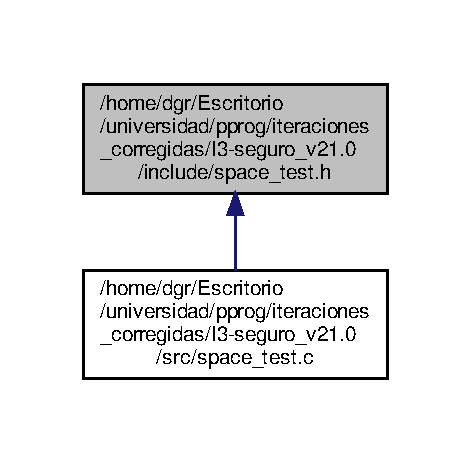
\includegraphics[width=226pt]{space__test_8h__dep__incl}
\end{center}
\end{figure}
\subsection*{Functions}
\begin{DoxyCompactItemize}
\item 
void \hyperlink{space__test_8h_a69278cc022dc5688d4725f8d36317b30}{test1\+\_\+space\+\_\+create} ()
\item 
void \hyperlink{space__test_8h_a012cd3cf37a8d91e2d7098a264c29d65}{test2\+\_\+space\+\_\+create} ()
\item 
void \hyperlink{space__test_8h_a2569bab6cfeec15f722d232bb8c78c9e}{test1\+\_\+space\+\_\+set\+\_\+name} ()
\item 
void \hyperlink{space__test_8h_a5a868ba017602ba6b58447cb394e81a6}{test2\+\_\+space\+\_\+set\+\_\+name} ()
\item 
void \hyperlink{space__test_8h_aa24a337830006e33706ab6ac1c416b47}{test3\+\_\+space\+\_\+set\+\_\+name} ()
\item 
void \hyperlink{space__test_8h_a3d3457a89f705948102cf1e5d4a7b45b}{test1\+\_\+space\+\_\+set\+\_\+north} ()
\item 
void \hyperlink{space__test_8h_a3bc7fe26c1e36ffd195099a9983206e1}{test2\+\_\+space\+\_\+set\+\_\+north} ()
\item 
void \hyperlink{space__test_8h_a21938e16547b3080e9251f960117a859}{test1\+\_\+space\+\_\+set\+\_\+south} ()
\item 
void \hyperlink{space__test_8h_ac9f950741f12ccfcc5ad5d9e71d3d90a}{test2\+\_\+space\+\_\+set\+\_\+south} ()
\item 
void \hyperlink{space__test_8h_ab1f093af4be3ca8e525d0517cc846f47}{test1\+\_\+space\+\_\+set\+\_\+east} ()
\item 
void \hyperlink{space__test_8h_a5df66d103388be4518c379b224f53770}{test2\+\_\+space\+\_\+set\+\_\+east} ()
\item 
void \hyperlink{space__test_8h_ab680a8797f793dffd58546074b87d21f}{test1\+\_\+space\+\_\+set\+\_\+west} ()
\item 
void \hyperlink{space__test_8h_aa51b05ffd99b7bbd8f2dfc23c8f85870}{test2\+\_\+space\+\_\+set\+\_\+west} ()
\item 
void \hyperlink{space__test_8h_a208ae9352ff979024f6ebef4e791356a}{test1\+\_\+space\+\_\+set\+\_\+object} ()
\item 
void \hyperlink{space__test_8h_a6349e2b547c71dee23b96d8bbf7a1806}{test2\+\_\+space\+\_\+set\+\_\+object} ()
\item 
void \hyperlink{space__test_8h_ad12c42523c517507566c5c68b1527689}{test1\+\_\+space\+\_\+get\+\_\+name} ()
\item 
void \hyperlink{space__test_8h_aee88ed31c63efc674051a4563aed86e2}{test2\+\_\+space\+\_\+get\+\_\+name} ()
\item 
void \hyperlink{space__test_8h_a4a1ca89fa511c04bb07c14edb19c17ba}{test1\+\_\+space\+\_\+get\+\_\+object} ()
\item 
void \hyperlink{space__test_8h_a0fe857c34f691aaba197d03315c3955f}{test2\+\_\+space\+\_\+get\+\_\+object} ()
\item 
void \hyperlink{space__test_8h_a3a87f1e1e173d622bfbd3bcd14e060ca}{test1\+\_\+space\+\_\+get\+\_\+north} ()
\item 
void \hyperlink{space__test_8h_a61891c9cebb9d26dc9f149ad8341517c}{test2\+\_\+space\+\_\+get\+\_\+north} ()
\item 
void \hyperlink{space__test_8h_a8e345065f58565e131bdb3a9d0096ed5}{test1\+\_\+space\+\_\+get\+\_\+south} ()
\item 
void \hyperlink{space__test_8h_a40fe07c07c1069023b362a9e506c4c59}{test2\+\_\+space\+\_\+get\+\_\+south} ()
\item 
void \hyperlink{space__test_8h_a354adb2722b06ec65b7212d2736d6417}{test1\+\_\+space\+\_\+get\+\_\+east} ()
\item 
void \hyperlink{space__test_8h_a249293510e61c6d5465f52c14343d02b}{test2\+\_\+space\+\_\+get\+\_\+east} ()
\item 
void \hyperlink{space__test_8h_a1f08c6866885bfc093717f57b1b86539}{test1\+\_\+space\+\_\+get\+\_\+west} ()
\item 
void \hyperlink{space__test_8h_af1cf02b01c007aec0684186b39666c32}{test2\+\_\+space\+\_\+get\+\_\+west} ()
\item 
void \hyperlink{space__test_8h_a920df9e02482f4f1e6a5ebcaec523860}{test1\+\_\+space\+\_\+get\+\_\+id} ()
\item 
void \hyperlink{space__test_8h_af9087176b0d3c41d83a17a4918b13e31}{test2\+\_\+space\+\_\+get\+\_\+id} ()
\end{DoxyCompactItemize}


\subsection{Detailed Description}
It declares the tests for the space module. 

\begin{DoxyAuthor}{Author}
Daniel Cerrato Sánchez 
\end{DoxyAuthor}
\begin{DoxyVersion}{Version}
3.\+0 
\end{DoxyVersion}
\begin{DoxyDate}{Date}
09-\/06-\/2020 
\end{DoxyDate}
\begin{DoxyCopyright}{Copyright}
G\+NU Public License 
\end{DoxyCopyright}


\subsection{Function Documentation}
\mbox{\Hypertarget{space__test_8h_a69278cc022dc5688d4725f8d36317b30}\label{space__test_8h_a69278cc022dc5688d4725f8d36317b30}} 
\index{space\+\_\+test.\+h@{space\+\_\+test.\+h}!test1\+\_\+space\+\_\+create@{test1\+\_\+space\+\_\+create}}
\index{test1\+\_\+space\+\_\+create@{test1\+\_\+space\+\_\+create}!space\+\_\+test.\+h@{space\+\_\+test.\+h}}
\subsubsection{\texorpdfstring{test1\+\_\+space\+\_\+create()}{test1\_space\_create()}}
{\footnotesize\ttfamily void test1\+\_\+space\+\_\+create (\begin{DoxyParamCaption}{ }\end{DoxyParamCaption})}

\begin{DoxyRefDesc}{Test}
\item[\hyperlink{test__test000151}{Test}]Test the space creation function \end{DoxyRefDesc}
\begin{DoxyPrecond}{Precondition}
An identifier as a parameter 
\end{DoxyPrecond}
\begin{DoxyPostcond}{Postcondition}
A non-\/null pointer to the created space 
\end{DoxyPostcond}
\mbox{\Hypertarget{space__test_8h_a354adb2722b06ec65b7212d2736d6417}\label{space__test_8h_a354adb2722b06ec65b7212d2736d6417}} 
\index{space\+\_\+test.\+h@{space\+\_\+test.\+h}!test1\+\_\+space\+\_\+get\+\_\+east@{test1\+\_\+space\+\_\+get\+\_\+east}}
\index{test1\+\_\+space\+\_\+get\+\_\+east@{test1\+\_\+space\+\_\+get\+\_\+east}!space\+\_\+test.\+h@{space\+\_\+test.\+h}}
\subsubsection{\texorpdfstring{test1\+\_\+space\+\_\+get\+\_\+east()}{test1\_space\_get\_east()}}
{\footnotesize\ttfamily void test1\+\_\+space\+\_\+get\+\_\+east (\begin{DoxyParamCaption}{ }\end{DoxyParamCaption})}

\begin{DoxyRefDesc}{Test}
\item[\hyperlink{test__test000174}{Test}]Test the function to get the east of a space \end{DoxyRefDesc}
\begin{DoxyPrecond}{Precondition}
Space is a non-\/\+N\+U\+LL pointer with space to the east 
\end{DoxyPrecond}
\begin{DoxyPostcond}{Postcondition}
The output must be the ide of the space to the east 
\end{DoxyPostcond}
\mbox{\Hypertarget{space__test_8h_a920df9e02482f4f1e6a5ebcaec523860}\label{space__test_8h_a920df9e02482f4f1e6a5ebcaec523860}} 
\index{space\+\_\+test.\+h@{space\+\_\+test.\+h}!test1\+\_\+space\+\_\+get\+\_\+id@{test1\+\_\+space\+\_\+get\+\_\+id}}
\index{test1\+\_\+space\+\_\+get\+\_\+id@{test1\+\_\+space\+\_\+get\+\_\+id}!space\+\_\+test.\+h@{space\+\_\+test.\+h}}
\subsubsection{\texorpdfstring{test1\+\_\+space\+\_\+get\+\_\+id()}{test1\_space\_get\_id()}}
{\footnotesize\ttfamily void test1\+\_\+space\+\_\+get\+\_\+id (\begin{DoxyParamCaption}{ }\end{DoxyParamCaption})}

\begin{DoxyRefDesc}{Test}
\item[\hyperlink{test__test000178}{Test}]Test the function to get the id of a space \end{DoxyRefDesc}
\begin{DoxyPrecond}{Precondition}
Space is a non-\/\+N\+U\+LL pointer with correct id 
\end{DoxyPrecond}
\begin{DoxyPostcond}{Postcondition}
The output must be the id provided 
\end{DoxyPostcond}
\mbox{\Hypertarget{space__test_8h_ad12c42523c517507566c5c68b1527689}\label{space__test_8h_ad12c42523c517507566c5c68b1527689}} 
\index{space\+\_\+test.\+h@{space\+\_\+test.\+h}!test1\+\_\+space\+\_\+get\+\_\+name@{test1\+\_\+space\+\_\+get\+\_\+name}}
\index{test1\+\_\+space\+\_\+get\+\_\+name@{test1\+\_\+space\+\_\+get\+\_\+name}!space\+\_\+test.\+h@{space\+\_\+test.\+h}}
\subsubsection{\texorpdfstring{test1\+\_\+space\+\_\+get\+\_\+name()}{test1\_space\_get\_name()}}
{\footnotesize\ttfamily void test1\+\_\+space\+\_\+get\+\_\+name (\begin{DoxyParamCaption}{ }\end{DoxyParamCaption})}

\begin{DoxyRefDesc}{Test}
\item[\hyperlink{test__test000166}{Test}]Test the function to get the name of a space \end{DoxyRefDesc}
\begin{DoxyPrecond}{Precondition}
Space is a non-\/\+N\+U\+LL named pointer 
\end{DoxyPrecond}
\begin{DoxyPostcond}{Postcondition}
The comparison between the last word and the name must be correct 
\end{DoxyPostcond}
\mbox{\Hypertarget{space__test_8h_a3a87f1e1e173d622bfbd3bcd14e060ca}\label{space__test_8h_a3a87f1e1e173d622bfbd3bcd14e060ca}} 
\index{space\+\_\+test.\+h@{space\+\_\+test.\+h}!test1\+\_\+space\+\_\+get\+\_\+north@{test1\+\_\+space\+\_\+get\+\_\+north}}
\index{test1\+\_\+space\+\_\+get\+\_\+north@{test1\+\_\+space\+\_\+get\+\_\+north}!space\+\_\+test.\+h@{space\+\_\+test.\+h}}
\subsubsection{\texorpdfstring{test1\+\_\+space\+\_\+get\+\_\+north()}{test1\_space\_get\_north()}}
{\footnotesize\ttfamily void test1\+\_\+space\+\_\+get\+\_\+north (\begin{DoxyParamCaption}{ }\end{DoxyParamCaption})}

\begin{DoxyRefDesc}{Test}
\item[\hyperlink{test__test000170}{Test}]Test the function to get the north of a space \end{DoxyRefDesc}
\begin{DoxyPrecond}{Precondition}
Space is a non-\/\+N\+U\+LL pointer with space to the north 
\end{DoxyPrecond}
\begin{DoxyPostcond}{Postcondition}
The output must be the id of the space to the north 
\end{DoxyPostcond}
\mbox{\Hypertarget{space__test_8h_a4a1ca89fa511c04bb07c14edb19c17ba}\label{space__test_8h_a4a1ca89fa511c04bb07c14edb19c17ba}} 
\index{space\+\_\+test.\+h@{space\+\_\+test.\+h}!test1\+\_\+space\+\_\+get\+\_\+object@{test1\+\_\+space\+\_\+get\+\_\+object}}
\index{test1\+\_\+space\+\_\+get\+\_\+object@{test1\+\_\+space\+\_\+get\+\_\+object}!space\+\_\+test.\+h@{space\+\_\+test.\+h}}
\subsubsection{\texorpdfstring{test1\+\_\+space\+\_\+get\+\_\+object()}{test1\_space\_get\_object()}}
{\footnotesize\ttfamily void test1\+\_\+space\+\_\+get\+\_\+object (\begin{DoxyParamCaption}{ }\end{DoxyParamCaption})}

\begin{DoxyRefDesc}{Test}
\item[\hyperlink{test__test000168}{Test}]Test the function to get the object set of a space \end{DoxyRefDesc}
\begin{DoxyPrecond}{Precondition}
The space is a non-\/\+N\+U\+LL pointer, but without adding objects 
\end{DoxyPrecond}
\begin{DoxyPostcond}{Postcondition}
The output must be different from N\+U\+LL 
\end{DoxyPostcond}
\mbox{\Hypertarget{space__test_8h_a8e345065f58565e131bdb3a9d0096ed5}\label{space__test_8h_a8e345065f58565e131bdb3a9d0096ed5}} 
\index{space\+\_\+test.\+h@{space\+\_\+test.\+h}!test1\+\_\+space\+\_\+get\+\_\+south@{test1\+\_\+space\+\_\+get\+\_\+south}}
\index{test1\+\_\+space\+\_\+get\+\_\+south@{test1\+\_\+space\+\_\+get\+\_\+south}!space\+\_\+test.\+h@{space\+\_\+test.\+h}}
\subsubsection{\texorpdfstring{test1\+\_\+space\+\_\+get\+\_\+south()}{test1\_space\_get\_south()}}
{\footnotesize\ttfamily void test1\+\_\+space\+\_\+get\+\_\+south (\begin{DoxyParamCaption}{ }\end{DoxyParamCaption})}

\begin{DoxyRefDesc}{Test}
\item[\hyperlink{test__test000172}{Test}]Test the function to get the south of a space \end{DoxyRefDesc}
\begin{DoxyPrecond}{Precondition}
Space is a non-\/\+N\+U\+LL pointer with space to the south 
\end{DoxyPrecond}
\begin{DoxyPostcond}{Postcondition}
The output must be the id of the space to the south 
\end{DoxyPostcond}
\mbox{\Hypertarget{space__test_8h_a1f08c6866885bfc093717f57b1b86539}\label{space__test_8h_a1f08c6866885bfc093717f57b1b86539}} 
\index{space\+\_\+test.\+h@{space\+\_\+test.\+h}!test1\+\_\+space\+\_\+get\+\_\+west@{test1\+\_\+space\+\_\+get\+\_\+west}}
\index{test1\+\_\+space\+\_\+get\+\_\+west@{test1\+\_\+space\+\_\+get\+\_\+west}!space\+\_\+test.\+h@{space\+\_\+test.\+h}}
\subsubsection{\texorpdfstring{test1\+\_\+space\+\_\+get\+\_\+west()}{test1\_space\_get\_west()}}
{\footnotesize\ttfamily void test1\+\_\+space\+\_\+get\+\_\+west (\begin{DoxyParamCaption}{ }\end{DoxyParamCaption})}

\begin{DoxyRefDesc}{Test}
\item[\hyperlink{test__test000176}{Test}]Test the function to get the west of a space \end{DoxyRefDesc}
\begin{DoxyPrecond}{Precondition}
Space is a non-\/\+N\+U\+LL pointer with space to the west 
\end{DoxyPrecond}
\begin{DoxyPostcond}{Postcondition}
The output must be the space id to the west 
\end{DoxyPostcond}
\mbox{\Hypertarget{space__test_8h_ab1f093af4be3ca8e525d0517cc846f47}\label{space__test_8h_ab1f093af4be3ca8e525d0517cc846f47}} 
\index{space\+\_\+test.\+h@{space\+\_\+test.\+h}!test1\+\_\+space\+\_\+set\+\_\+east@{test1\+\_\+space\+\_\+set\+\_\+east}}
\index{test1\+\_\+space\+\_\+set\+\_\+east@{test1\+\_\+space\+\_\+set\+\_\+east}!space\+\_\+test.\+h@{space\+\_\+test.\+h}}
\subsubsection{\texorpdfstring{test1\+\_\+space\+\_\+set\+\_\+east()}{test1\_space\_set\_east()}}
{\footnotesize\ttfamily void test1\+\_\+space\+\_\+set\+\_\+east (\begin{DoxyParamCaption}{ }\end{DoxyParamCaption})}

\begin{DoxyRefDesc}{Test}
\item[\hyperlink{test__test000160}{Test}]Test the function to set the east of a space \end{DoxyRefDesc}
\begin{DoxyPrecond}{Precondition}
The space is a non-\/\+N\+U\+LL pointer and the id is correct 
\end{DoxyPrecond}
\begin{DoxyPostcond}{Postcondition}
The output must be OK 
\end{DoxyPostcond}
\mbox{\Hypertarget{space__test_8h_a2569bab6cfeec15f722d232bb8c78c9e}\label{space__test_8h_a2569bab6cfeec15f722d232bb8c78c9e}} 
\index{space\+\_\+test.\+h@{space\+\_\+test.\+h}!test1\+\_\+space\+\_\+set\+\_\+name@{test1\+\_\+space\+\_\+set\+\_\+name}}
\index{test1\+\_\+space\+\_\+set\+\_\+name@{test1\+\_\+space\+\_\+set\+\_\+name}!space\+\_\+test.\+h@{space\+\_\+test.\+h}}
\subsubsection{\texorpdfstring{test1\+\_\+space\+\_\+set\+\_\+name()}{test1\_space\_set\_name()}}
{\footnotesize\ttfamily void test1\+\_\+space\+\_\+set\+\_\+name (\begin{DoxyParamCaption}{ }\end{DoxyParamCaption})}

\begin{DoxyRefDesc}{Test}
\item[\hyperlink{test__test000153}{Test}]Test the function to set the name of a space \end{DoxyRefDesc}
\begin{DoxyPrecond}{Precondition}
Name to set the space 
\end{DoxyPrecond}
\begin{DoxyPostcond}{Postcondition}
The output must be OK 
\end{DoxyPostcond}
\mbox{\Hypertarget{space__test_8h_a3d3457a89f705948102cf1e5d4a7b45b}\label{space__test_8h_a3d3457a89f705948102cf1e5d4a7b45b}} 
\index{space\+\_\+test.\+h@{space\+\_\+test.\+h}!test1\+\_\+space\+\_\+set\+\_\+north@{test1\+\_\+space\+\_\+set\+\_\+north}}
\index{test1\+\_\+space\+\_\+set\+\_\+north@{test1\+\_\+space\+\_\+set\+\_\+north}!space\+\_\+test.\+h@{space\+\_\+test.\+h}}
\subsubsection{\texorpdfstring{test1\+\_\+space\+\_\+set\+\_\+north()}{test1\_space\_set\_north()}}
{\footnotesize\ttfamily void test1\+\_\+space\+\_\+set\+\_\+north (\begin{DoxyParamCaption}{ }\end{DoxyParamCaption})}

\begin{DoxyRefDesc}{Test}
\item[\hyperlink{test__test000156}{Test}]Test the function to set the north of a space \end{DoxyRefDesc}
\begin{DoxyPrecond}{Precondition}
The space is a non-\/\+N\+U\+LL pointer and the id is correct 
\end{DoxyPrecond}
\begin{DoxyPostcond}{Postcondition}
The output must be OK 
\end{DoxyPostcond}
\mbox{\Hypertarget{space__test_8h_a208ae9352ff979024f6ebef4e791356a}\label{space__test_8h_a208ae9352ff979024f6ebef4e791356a}} 
\index{space\+\_\+test.\+h@{space\+\_\+test.\+h}!test1\+\_\+space\+\_\+set\+\_\+object@{test1\+\_\+space\+\_\+set\+\_\+object}}
\index{test1\+\_\+space\+\_\+set\+\_\+object@{test1\+\_\+space\+\_\+set\+\_\+object}!space\+\_\+test.\+h@{space\+\_\+test.\+h}}
\subsubsection{\texorpdfstring{test1\+\_\+space\+\_\+set\+\_\+object()}{test1\_space\_set\_object()}}
{\footnotesize\ttfamily void test1\+\_\+space\+\_\+set\+\_\+object (\begin{DoxyParamCaption}{ }\end{DoxyParamCaption})}

\begin{DoxyRefDesc}{Test}
\item[\hyperlink{test__test000164}{Test}]Test the function to set objects in a space \end{DoxyRefDesc}
\begin{DoxyPrecond}{Precondition}
The space is a non-\/\+N\+U\+LL pointer and is passed a correct id 
\end{DoxyPrecond}
\begin{DoxyPostcond}{Postcondition}
The output must be OK 
\end{DoxyPostcond}
\mbox{\Hypertarget{space__test_8h_a21938e16547b3080e9251f960117a859}\label{space__test_8h_a21938e16547b3080e9251f960117a859}} 
\index{space\+\_\+test.\+h@{space\+\_\+test.\+h}!test1\+\_\+space\+\_\+set\+\_\+south@{test1\+\_\+space\+\_\+set\+\_\+south}}
\index{test1\+\_\+space\+\_\+set\+\_\+south@{test1\+\_\+space\+\_\+set\+\_\+south}!space\+\_\+test.\+h@{space\+\_\+test.\+h}}
\subsubsection{\texorpdfstring{test1\+\_\+space\+\_\+set\+\_\+south()}{test1\_space\_set\_south()}}
{\footnotesize\ttfamily void test1\+\_\+space\+\_\+set\+\_\+south (\begin{DoxyParamCaption}{ }\end{DoxyParamCaption})}

\begin{DoxyRefDesc}{Test}
\item[\hyperlink{test__test000158}{Test}]Test the function to set the south of a space \end{DoxyRefDesc}
\begin{DoxyPrecond}{Precondition}
The space is a non-\/\+N\+U\+LL pointer and the id is correct 
\end{DoxyPrecond}
\begin{DoxyPostcond}{Postcondition}
The output must be OK 
\end{DoxyPostcond}
\mbox{\Hypertarget{space__test_8h_ab680a8797f793dffd58546074b87d21f}\label{space__test_8h_ab680a8797f793dffd58546074b87d21f}} 
\index{space\+\_\+test.\+h@{space\+\_\+test.\+h}!test1\+\_\+space\+\_\+set\+\_\+west@{test1\+\_\+space\+\_\+set\+\_\+west}}
\index{test1\+\_\+space\+\_\+set\+\_\+west@{test1\+\_\+space\+\_\+set\+\_\+west}!space\+\_\+test.\+h@{space\+\_\+test.\+h}}
\subsubsection{\texorpdfstring{test1\+\_\+space\+\_\+set\+\_\+west()}{test1\_space\_set\_west()}}
{\footnotesize\ttfamily void test1\+\_\+space\+\_\+set\+\_\+west (\begin{DoxyParamCaption}{ }\end{DoxyParamCaption})}

\begin{DoxyRefDesc}{Test}
\item[\hyperlink{test__test000162}{Test}]Test the function to set the west of a space \end{DoxyRefDesc}
\begin{DoxyPrecond}{Precondition}
The space is a non-\/\+N\+U\+LL pointer and the id is correct 
\end{DoxyPrecond}
\begin{DoxyPostcond}{Postcondition}
The output must be OK 
\end{DoxyPostcond}
\mbox{\Hypertarget{space__test_8h_a012cd3cf37a8d91e2d7098a264c29d65}\label{space__test_8h_a012cd3cf37a8d91e2d7098a264c29d65}} 
\index{space\+\_\+test.\+h@{space\+\_\+test.\+h}!test2\+\_\+space\+\_\+create@{test2\+\_\+space\+\_\+create}}
\index{test2\+\_\+space\+\_\+create@{test2\+\_\+space\+\_\+create}!space\+\_\+test.\+h@{space\+\_\+test.\+h}}
\subsubsection{\texorpdfstring{test2\+\_\+space\+\_\+create()}{test2\_space\_create()}}
{\footnotesize\ttfamily void test2\+\_\+space\+\_\+create (\begin{DoxyParamCaption}{ }\end{DoxyParamCaption})}

\begin{DoxyRefDesc}{Test}
\item[\hyperlink{test__test000152}{Test}]Test the space creation function \end{DoxyRefDesc}
\begin{DoxyPrecond}{Precondition}
An identifier as a parameter 
\end{DoxyPrecond}
\begin{DoxyPostcond}{Postcondition}
The space identifier is the one entered 
\end{DoxyPostcond}
\mbox{\Hypertarget{space__test_8h_a249293510e61c6d5465f52c14343d02b}\label{space__test_8h_a249293510e61c6d5465f52c14343d02b}} 
\index{space\+\_\+test.\+h@{space\+\_\+test.\+h}!test2\+\_\+space\+\_\+get\+\_\+east@{test2\+\_\+space\+\_\+get\+\_\+east}}
\index{test2\+\_\+space\+\_\+get\+\_\+east@{test2\+\_\+space\+\_\+get\+\_\+east}!space\+\_\+test.\+h@{space\+\_\+test.\+h}}
\subsubsection{\texorpdfstring{test2\+\_\+space\+\_\+get\+\_\+east()}{test2\_space\_get\_east()}}
{\footnotesize\ttfamily void test2\+\_\+space\+\_\+get\+\_\+east (\begin{DoxyParamCaption}{ }\end{DoxyParamCaption})}

\begin{DoxyRefDesc}{Test}
\item[\hyperlink{test__test000175}{Test}]Test the function to get the south of a space \end{DoxyRefDesc}
\begin{DoxyPrecond}{Precondition}
Space is a pointer to N\+U\+LL 
\end{DoxyPrecond}
\begin{DoxyPostcond}{Postcondition}
The output must be N\+O\+\_\+\+ID 
\end{DoxyPostcond}
\mbox{\Hypertarget{space__test_8h_af9087176b0d3c41d83a17a4918b13e31}\label{space__test_8h_af9087176b0d3c41d83a17a4918b13e31}} 
\index{space\+\_\+test.\+h@{space\+\_\+test.\+h}!test2\+\_\+space\+\_\+get\+\_\+id@{test2\+\_\+space\+\_\+get\+\_\+id}}
\index{test2\+\_\+space\+\_\+get\+\_\+id@{test2\+\_\+space\+\_\+get\+\_\+id}!space\+\_\+test.\+h@{space\+\_\+test.\+h}}
\subsubsection{\texorpdfstring{test2\+\_\+space\+\_\+get\+\_\+id()}{test2\_space\_get\_id()}}
{\footnotesize\ttfamily void test2\+\_\+space\+\_\+get\+\_\+id (\begin{DoxyParamCaption}{ }\end{DoxyParamCaption})}

\begin{DoxyRefDesc}{Test}
\item[\hyperlink{test__test000179}{Test}]Test the function to get the id of a space \end{DoxyRefDesc}
\begin{DoxyPrecond}{Precondition}
Space is a pointer to N\+U\+LL 
\end{DoxyPrecond}
\begin{DoxyPostcond}{Postcondition}
The output must be N\+O\+\_\+\+ID 
\end{DoxyPostcond}
\mbox{\Hypertarget{space__test_8h_aee88ed31c63efc674051a4563aed86e2}\label{space__test_8h_aee88ed31c63efc674051a4563aed86e2}} 
\index{space\+\_\+test.\+h@{space\+\_\+test.\+h}!test2\+\_\+space\+\_\+get\+\_\+name@{test2\+\_\+space\+\_\+get\+\_\+name}}
\index{test2\+\_\+space\+\_\+get\+\_\+name@{test2\+\_\+space\+\_\+get\+\_\+name}!space\+\_\+test.\+h@{space\+\_\+test.\+h}}
\subsubsection{\texorpdfstring{test2\+\_\+space\+\_\+get\+\_\+name()}{test2\_space\_get\_name()}}
{\footnotesize\ttfamily void test2\+\_\+space\+\_\+get\+\_\+name (\begin{DoxyParamCaption}{ }\end{DoxyParamCaption})}

\begin{DoxyRefDesc}{Test}
\item[\hyperlink{test__test000167}{Test}]Test the function to get the name of a space \end{DoxyRefDesc}
\begin{DoxyPrecond}{Precondition}
Space is a pointer to N\+U\+LL 
\end{DoxyPrecond}
\begin{DoxyPostcond}{Postcondition}
The output must be N\+U\+LL 
\end{DoxyPostcond}
\mbox{\Hypertarget{space__test_8h_a61891c9cebb9d26dc9f149ad8341517c}\label{space__test_8h_a61891c9cebb9d26dc9f149ad8341517c}} 
\index{space\+\_\+test.\+h@{space\+\_\+test.\+h}!test2\+\_\+space\+\_\+get\+\_\+north@{test2\+\_\+space\+\_\+get\+\_\+north}}
\index{test2\+\_\+space\+\_\+get\+\_\+north@{test2\+\_\+space\+\_\+get\+\_\+north}!space\+\_\+test.\+h@{space\+\_\+test.\+h}}
\subsubsection{\texorpdfstring{test2\+\_\+space\+\_\+get\+\_\+north()}{test2\_space\_get\_north()}}
{\footnotesize\ttfamily void test2\+\_\+space\+\_\+get\+\_\+north (\begin{DoxyParamCaption}{ }\end{DoxyParamCaption})}

\begin{DoxyRefDesc}{Test}
\item[\hyperlink{test__test000171}{Test}]Test the function to get the north of a space \end{DoxyRefDesc}
\begin{DoxyPrecond}{Precondition}
Space is a pointer to N\+U\+LL 
\end{DoxyPrecond}
\begin{DoxyPostcond}{Postcondition}
The output must be N\+O\+\_\+\+ID 
\end{DoxyPostcond}
\mbox{\Hypertarget{space__test_8h_a0fe857c34f691aaba197d03315c3955f}\label{space__test_8h_a0fe857c34f691aaba197d03315c3955f}} 
\index{space\+\_\+test.\+h@{space\+\_\+test.\+h}!test2\+\_\+space\+\_\+get\+\_\+object@{test2\+\_\+space\+\_\+get\+\_\+object}}
\index{test2\+\_\+space\+\_\+get\+\_\+object@{test2\+\_\+space\+\_\+get\+\_\+object}!space\+\_\+test.\+h@{space\+\_\+test.\+h}}
\subsubsection{\texorpdfstring{test2\+\_\+space\+\_\+get\+\_\+object()}{test2\_space\_get\_object()}}
{\footnotesize\ttfamily void test2\+\_\+space\+\_\+get\+\_\+object (\begin{DoxyParamCaption}{ }\end{DoxyParamCaption})}

\begin{DoxyRefDesc}{Test}
\item[\hyperlink{test__test000169}{Test}]Test the function to get the object of a space \end{DoxyRefDesc}
\begin{DoxyPrecond}{Precondition}
Space is a pointer to N\+U\+LL 
\end{DoxyPrecond}
\begin{DoxyPostcond}{Postcondition}
The output must be N\+U\+LL 
\end{DoxyPostcond}
\mbox{\Hypertarget{space__test_8h_a40fe07c07c1069023b362a9e506c4c59}\label{space__test_8h_a40fe07c07c1069023b362a9e506c4c59}} 
\index{space\+\_\+test.\+h@{space\+\_\+test.\+h}!test2\+\_\+space\+\_\+get\+\_\+south@{test2\+\_\+space\+\_\+get\+\_\+south}}
\index{test2\+\_\+space\+\_\+get\+\_\+south@{test2\+\_\+space\+\_\+get\+\_\+south}!space\+\_\+test.\+h@{space\+\_\+test.\+h}}
\subsubsection{\texorpdfstring{test2\+\_\+space\+\_\+get\+\_\+south()}{test2\_space\_get\_south()}}
{\footnotesize\ttfamily void test2\+\_\+space\+\_\+get\+\_\+south (\begin{DoxyParamCaption}{ }\end{DoxyParamCaption})}

\begin{DoxyRefDesc}{Test}
\item[\hyperlink{test__test000173}{Test}]Test the function to get the south of a space \end{DoxyRefDesc}
\begin{DoxyPrecond}{Precondition}
Space is a pointer to N\+U\+LL 
\end{DoxyPrecond}
\begin{DoxyPostcond}{Postcondition}
The output must be N\+O\+\_\+\+ID 
\end{DoxyPostcond}
\mbox{\Hypertarget{space__test_8h_af1cf02b01c007aec0684186b39666c32}\label{space__test_8h_af1cf02b01c007aec0684186b39666c32}} 
\index{space\+\_\+test.\+h@{space\+\_\+test.\+h}!test2\+\_\+space\+\_\+get\+\_\+west@{test2\+\_\+space\+\_\+get\+\_\+west}}
\index{test2\+\_\+space\+\_\+get\+\_\+west@{test2\+\_\+space\+\_\+get\+\_\+west}!space\+\_\+test.\+h@{space\+\_\+test.\+h}}
\subsubsection{\texorpdfstring{test2\+\_\+space\+\_\+get\+\_\+west()}{test2\_space\_get\_west()}}
{\footnotesize\ttfamily void test2\+\_\+space\+\_\+get\+\_\+west (\begin{DoxyParamCaption}{ }\end{DoxyParamCaption})}

\begin{DoxyRefDesc}{Test}
\item[\hyperlink{test__test000177}{Test}]Test the function to get the south of a space \end{DoxyRefDesc}
\begin{DoxyPrecond}{Precondition}
Space is a pointer to N\+U\+LL 
\end{DoxyPrecond}
\begin{DoxyPostcond}{Postcondition}
The output must be N\+O\+\_\+\+ID 
\end{DoxyPostcond}
\mbox{\Hypertarget{space__test_8h_a5df66d103388be4518c379b224f53770}\label{space__test_8h_a5df66d103388be4518c379b224f53770}} 
\index{space\+\_\+test.\+h@{space\+\_\+test.\+h}!test2\+\_\+space\+\_\+set\+\_\+east@{test2\+\_\+space\+\_\+set\+\_\+east}}
\index{test2\+\_\+space\+\_\+set\+\_\+east@{test2\+\_\+space\+\_\+set\+\_\+east}!space\+\_\+test.\+h@{space\+\_\+test.\+h}}
\subsubsection{\texorpdfstring{test2\+\_\+space\+\_\+set\+\_\+east()}{test2\_space\_set\_east()}}
{\footnotesize\ttfamily void test2\+\_\+space\+\_\+set\+\_\+east (\begin{DoxyParamCaption}{ }\end{DoxyParamCaption})}

\begin{DoxyRefDesc}{Test}
\item[\hyperlink{test__test000161}{Test}]Test the function to set the east of a space \end{DoxyRefDesc}
\begin{DoxyPrecond}{Precondition}
Space is a pointer to N\+U\+LL 
\end{DoxyPrecond}
\begin{DoxyPostcond}{Postcondition}
The output must be E\+R\+R\+OR 
\end{DoxyPostcond}
\mbox{\Hypertarget{space__test_8h_a5a868ba017602ba6b58447cb394e81a6}\label{space__test_8h_a5a868ba017602ba6b58447cb394e81a6}} 
\index{space\+\_\+test.\+h@{space\+\_\+test.\+h}!test2\+\_\+space\+\_\+set\+\_\+name@{test2\+\_\+space\+\_\+set\+\_\+name}}
\index{test2\+\_\+space\+\_\+set\+\_\+name@{test2\+\_\+space\+\_\+set\+\_\+name}!space\+\_\+test.\+h@{space\+\_\+test.\+h}}
\subsubsection{\texorpdfstring{test2\+\_\+space\+\_\+set\+\_\+name()}{test2\_space\_set\_name()}}
{\footnotesize\ttfamily void test2\+\_\+space\+\_\+set\+\_\+name (\begin{DoxyParamCaption}{ }\end{DoxyParamCaption})}

\begin{DoxyRefDesc}{Test}
\item[\hyperlink{test__test000154}{Test}]Test the function to set the name of a space \end{DoxyRefDesc}
\begin{DoxyPrecond}{Precondition}
The space to set the name to is a pointer to N\+U\+LL 
\end{DoxyPrecond}
\begin{DoxyPostcond}{Postcondition}
The output must be E\+R\+R\+OR 
\end{DoxyPostcond}
\mbox{\Hypertarget{space__test_8h_a3bc7fe26c1e36ffd195099a9983206e1}\label{space__test_8h_a3bc7fe26c1e36ffd195099a9983206e1}} 
\index{space\+\_\+test.\+h@{space\+\_\+test.\+h}!test2\+\_\+space\+\_\+set\+\_\+north@{test2\+\_\+space\+\_\+set\+\_\+north}}
\index{test2\+\_\+space\+\_\+set\+\_\+north@{test2\+\_\+space\+\_\+set\+\_\+north}!space\+\_\+test.\+h@{space\+\_\+test.\+h}}
\subsubsection{\texorpdfstring{test2\+\_\+space\+\_\+set\+\_\+north()}{test2\_space\_set\_north()}}
{\footnotesize\ttfamily void test2\+\_\+space\+\_\+set\+\_\+north (\begin{DoxyParamCaption}{ }\end{DoxyParamCaption})}

\begin{DoxyRefDesc}{Test}
\item[\hyperlink{test__test000157}{Test}]Test the function to set the north of a space \end{DoxyRefDesc}
\begin{DoxyPrecond}{Precondition}
Space is a pointer to N\+U\+LL 
\end{DoxyPrecond}
\begin{DoxyPostcond}{Postcondition}
The output must be E\+R\+R\+OR 
\end{DoxyPostcond}
\mbox{\Hypertarget{space__test_8h_a6349e2b547c71dee23b96d8bbf7a1806}\label{space__test_8h_a6349e2b547c71dee23b96d8bbf7a1806}} 
\index{space\+\_\+test.\+h@{space\+\_\+test.\+h}!test2\+\_\+space\+\_\+set\+\_\+object@{test2\+\_\+space\+\_\+set\+\_\+object}}
\index{test2\+\_\+space\+\_\+set\+\_\+object@{test2\+\_\+space\+\_\+set\+\_\+object}!space\+\_\+test.\+h@{space\+\_\+test.\+h}}
\subsubsection{\texorpdfstring{test2\+\_\+space\+\_\+set\+\_\+object()}{test2\_space\_set\_object()}}
{\footnotesize\ttfamily void test2\+\_\+space\+\_\+set\+\_\+object (\begin{DoxyParamCaption}{ }\end{DoxyParamCaption})}

\begin{DoxyRefDesc}{Test}
\item[\hyperlink{test__test000165}{Test}]Test the function to set objects in a space \end{DoxyRefDesc}
\begin{DoxyPrecond}{Precondition}
Space is a pointer to N\+U\+LL 
\end{DoxyPrecond}
\begin{DoxyPostcond}{Postcondition}
The output must be E\+R\+R\+OR 
\end{DoxyPostcond}
\mbox{\Hypertarget{space__test_8h_ac9f950741f12ccfcc5ad5d9e71d3d90a}\label{space__test_8h_ac9f950741f12ccfcc5ad5d9e71d3d90a}} 
\index{space\+\_\+test.\+h@{space\+\_\+test.\+h}!test2\+\_\+space\+\_\+set\+\_\+south@{test2\+\_\+space\+\_\+set\+\_\+south}}
\index{test2\+\_\+space\+\_\+set\+\_\+south@{test2\+\_\+space\+\_\+set\+\_\+south}!space\+\_\+test.\+h@{space\+\_\+test.\+h}}
\subsubsection{\texorpdfstring{test2\+\_\+space\+\_\+set\+\_\+south()}{test2\_space\_set\_south()}}
{\footnotesize\ttfamily void test2\+\_\+space\+\_\+set\+\_\+south (\begin{DoxyParamCaption}{ }\end{DoxyParamCaption})}

\begin{DoxyRefDesc}{Test}
\item[\hyperlink{test__test000159}{Test}]Test the function to set the south of a space \end{DoxyRefDesc}
\begin{DoxyPrecond}{Precondition}
Space is a pointer to N\+U\+LL 
\end{DoxyPrecond}
\begin{DoxyPostcond}{Postcondition}
The output must be E\+R\+R\+OR 
\end{DoxyPostcond}
\mbox{\Hypertarget{space__test_8h_aa51b05ffd99b7bbd8f2dfc23c8f85870}\label{space__test_8h_aa51b05ffd99b7bbd8f2dfc23c8f85870}} 
\index{space\+\_\+test.\+h@{space\+\_\+test.\+h}!test2\+\_\+space\+\_\+set\+\_\+west@{test2\+\_\+space\+\_\+set\+\_\+west}}
\index{test2\+\_\+space\+\_\+set\+\_\+west@{test2\+\_\+space\+\_\+set\+\_\+west}!space\+\_\+test.\+h@{space\+\_\+test.\+h}}
\subsubsection{\texorpdfstring{test2\+\_\+space\+\_\+set\+\_\+west()}{test2\_space\_set\_west()}}
{\footnotesize\ttfamily void test2\+\_\+space\+\_\+set\+\_\+west (\begin{DoxyParamCaption}{ }\end{DoxyParamCaption})}

\begin{DoxyRefDesc}{Test}
\item[\hyperlink{test__test000163}{Test}]Test the function to set the west of a space \end{DoxyRefDesc}
\begin{DoxyPrecond}{Precondition}
Space is a pointer to N\+U\+LL 
\end{DoxyPrecond}
\begin{DoxyPostcond}{Postcondition}
The output must be E\+R\+R\+OR 
\end{DoxyPostcond}
\mbox{\Hypertarget{space__test_8h_aa24a337830006e33706ab6ac1c416b47}\label{space__test_8h_aa24a337830006e33706ab6ac1c416b47}} 
\index{space\+\_\+test.\+h@{space\+\_\+test.\+h}!test3\+\_\+space\+\_\+set\+\_\+name@{test3\+\_\+space\+\_\+set\+\_\+name}}
\index{test3\+\_\+space\+\_\+set\+\_\+name@{test3\+\_\+space\+\_\+set\+\_\+name}!space\+\_\+test.\+h@{space\+\_\+test.\+h}}
\subsubsection{\texorpdfstring{test3\+\_\+space\+\_\+set\+\_\+name()}{test3\_space\_set\_name()}}
{\footnotesize\ttfamily void test3\+\_\+space\+\_\+set\+\_\+name (\begin{DoxyParamCaption}{ }\end{DoxyParamCaption})}

\begin{DoxyRefDesc}{Test}
\item[\hyperlink{test__test000155}{Test}]Test the function to set the name of a space \end{DoxyRefDesc}
\begin{DoxyPrecond}{Precondition}
The space is a non-\/\+N\+U\+LL pointer, but the name to set is N\+U\+LL 
\end{DoxyPrecond}
\begin{DoxyPostcond}{Postcondition}
The output must be E\+R\+R\+OR 
\end{DoxyPostcond}

\hypertarget{types_8h}{}\section{/home/dgr/\+Escritorio/universidad/pprog/iteraciones\+\_\+corregidas/\+I3-\/seguro\+\_\+v21.0/include/types.h File Reference}
\label{types_8h}\index{/home/dgr/\+Escritorio/universidad/pprog/iteraciones\+\_\+corregidas/\+I3-\/seguro\+\_\+v21.\+0/include/types.\+h@{/home/dgr/\+Escritorio/universidad/pprog/iteraciones\+\_\+corregidas/\+I3-\/seguro\+\_\+v21.\+0/include/types.\+h}}


It defines common types.  


This graph shows which files directly or indirectly include this file\+:
\nopagebreak
\begin{figure}[H]
\begin{center}
\leavevmode
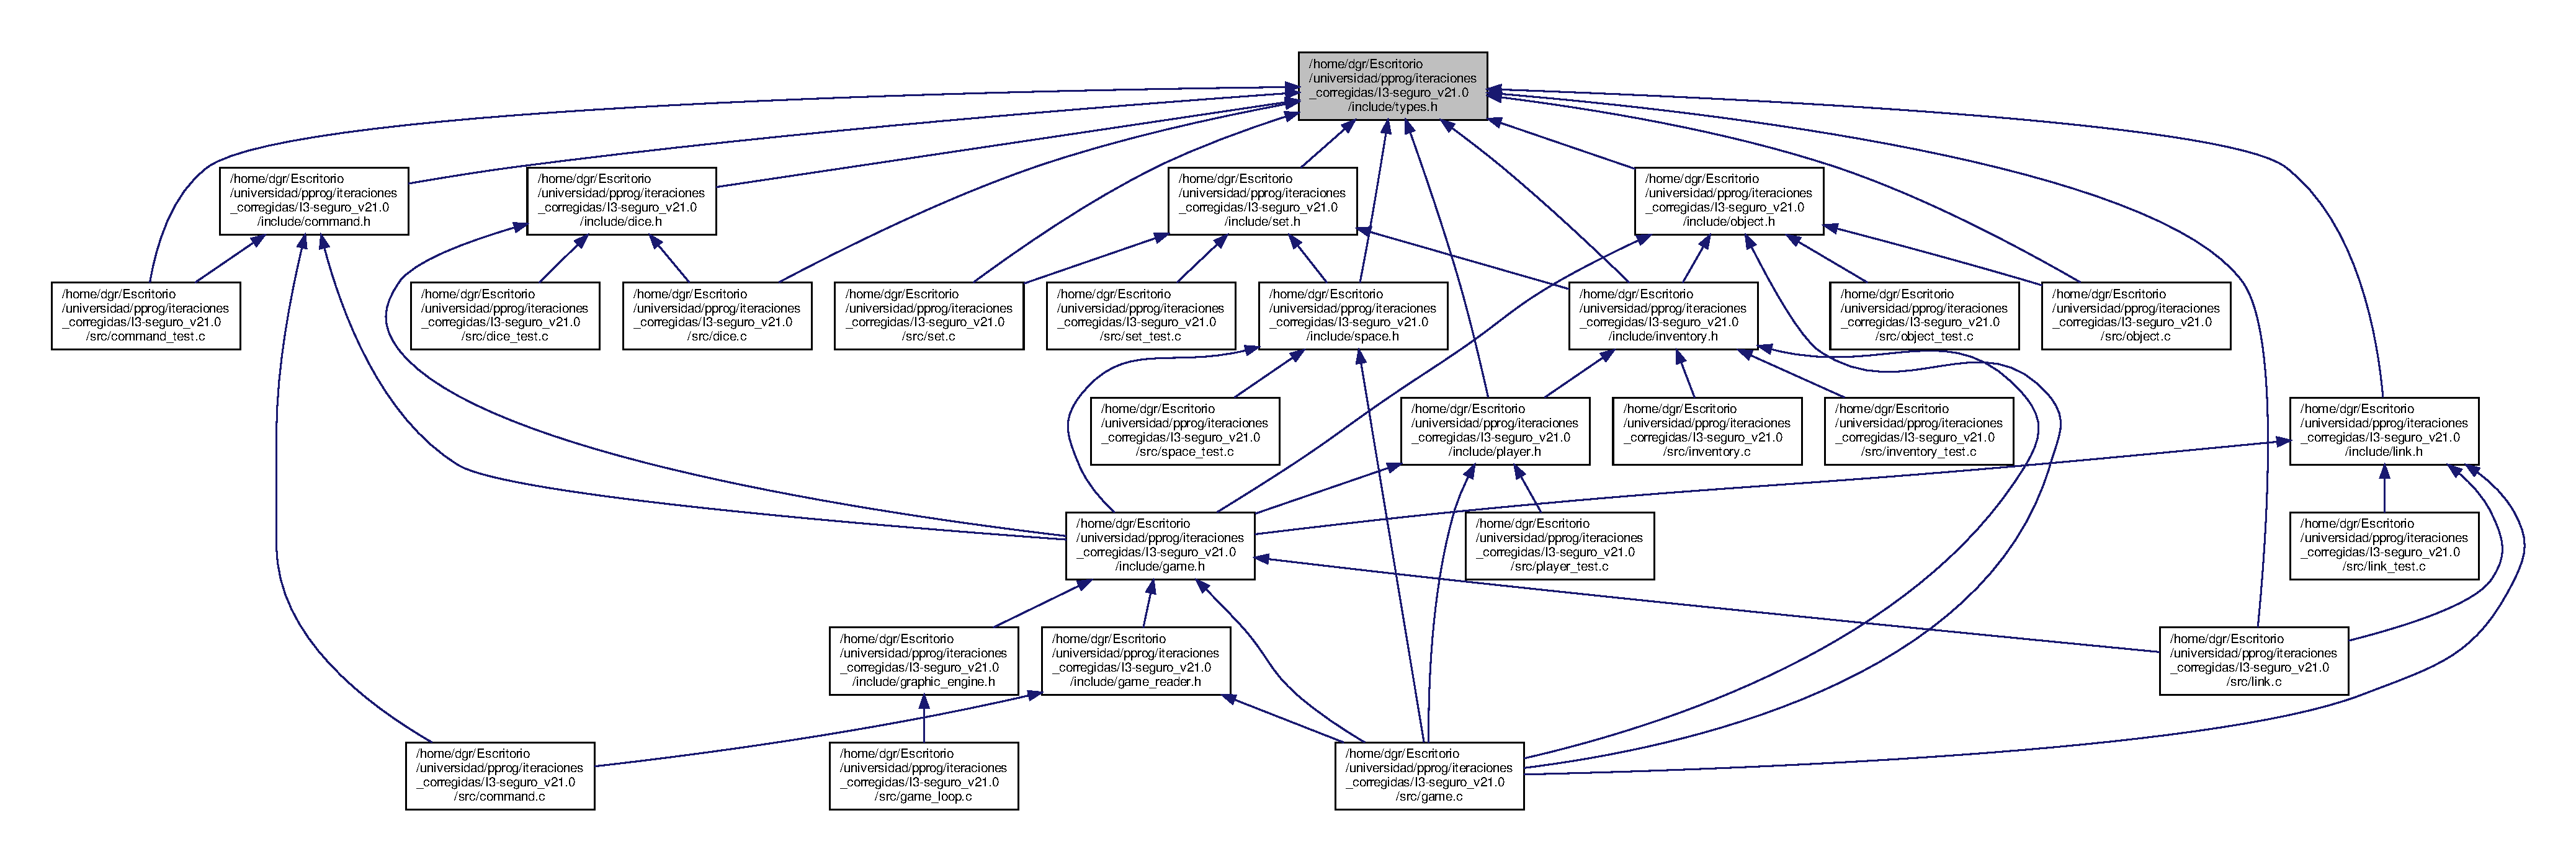
\includegraphics[width=350pt]{types_8h__dep__incl}
\end{center}
\end{figure}
\subsection*{Macros}
\begin{DoxyCompactItemize}
\item 
\#define \hyperlink{types_8h_a92ed8507d1cd2331ad09275c5c4c1c89}{W\+O\+R\+D\+\_\+\+S\+I\+ZE}~1000
\begin{DoxyCompactList}\small\item\em A macro that stores the word size. \end{DoxyCompactList}\item 
\#define \hyperlink{types_8h_a642e16f35aa1e585c25e405ede76e115}{N\+O\+\_\+\+ID}~-\/1
\begin{DoxyCompactList}\small\item\em A macro that define no id. \end{DoxyCompactList}\end{DoxyCompactItemize}
\subsection*{Typedefs}
\begin{DoxyCompactItemize}
\item 
typedef long \hyperlink{types_8h_a845e604fb28f7e3d97549da3448149d3}{Id}
\begin{DoxyCompactList}\small\item\em A type definition for a id. \end{DoxyCompactList}\end{DoxyCompactItemize}
\subsection*{Enumerations}
\begin{DoxyCompactItemize}
\item 
enum \hyperlink{types_8h_a3e5b8192e7d9ffaf3542f1210aec18dd}{B\+O\+OL} \{ \hyperlink{types_8h_a3e5b8192e7d9ffaf3542f1210aec18ddaa1e095cc966dbecf6a0d8aad75348d1a}{F\+A\+L\+SE}, 
\hyperlink{types_8h_a3e5b8192e7d9ffaf3542f1210aec18ddaa82764c3079aea4e60c80e45befbb839}{T\+R\+UE}
 \}\begin{DoxyCompactList}\small\item\em The Boolean enum. \end{DoxyCompactList}
\item 
enum \hyperlink{types_8h_a32c27cc471df37f4fc818d65de0a56c4}{S\+T\+A\+T\+US} \{ \hyperlink{types_8h_a32c27cc471df37f4fc818d65de0a56c4a2fd6f336d08340583bd620a7f5694c90}{E\+R\+R\+OR}, 
\hyperlink{types_8h_a32c27cc471df37f4fc818d65de0a56c4a2bc49ec37d6a5715dd23e85f1ff5bb59}{OK}
 \}\begin{DoxyCompactList}\small\item\em The Status enum. \end{DoxyCompactList}
\item 
enum \hyperlink{types_8h_aa268a41a13430b18e933ed40207178d0}{D\+I\+R\+E\+C\+T\+I\+ON} \{ \hyperlink{types_8h_aa268a41a13430b18e933ed40207178d0a2c63acbe79d9f41ba6bb7766e9c37702}{N}, 
\hyperlink{types_8h_aa268a41a13430b18e933ed40207178d0af1ce01387d2348f8b858721a7db81670}{S}, 
\hyperlink{types_8h_aa268a41a13430b18e933ed40207178d0ab199e021998d49b1f09338d8b9b18ecb}{E}, 
\hyperlink{types_8h_aa268a41a13430b18e933ed40207178d0ab722ceeb601c72cd78fbd35f3581fdf7}{W}
 \}\begin{DoxyCompactList}\small\item\em The Direction enum. \end{DoxyCompactList}
\end{DoxyCompactItemize}


\subsection{Detailed Description}
It defines common types. 

\begin{DoxyAuthor}{Author}
Profesores P\+P\+R\+OG 
\end{DoxyAuthor}
\begin{DoxyVersion}{Version}
1.\+0 
\end{DoxyVersion}
\begin{DoxyDate}{Date}
13-\/01-\/2015 
\end{DoxyDate}
\begin{DoxyCopyright}{Copyright}
G\+NU Public License 
\end{DoxyCopyright}


\subsection{Macro Definition Documentation}
\mbox{\Hypertarget{types_8h_a642e16f35aa1e585c25e405ede76e115}\label{types_8h_a642e16f35aa1e585c25e405ede76e115}} 
\index{types.\+h@{types.\+h}!N\+O\+\_\+\+ID@{N\+O\+\_\+\+ID}}
\index{N\+O\+\_\+\+ID@{N\+O\+\_\+\+ID}!types.\+h@{types.\+h}}
\subsubsection{\texorpdfstring{N\+O\+\_\+\+ID}{NO\_ID}}
{\footnotesize\ttfamily \#define N\+O\+\_\+\+ID~-\/1}



A macro that define no id. 

Details. \mbox{\Hypertarget{types_8h_a92ed8507d1cd2331ad09275c5c4c1c89}\label{types_8h_a92ed8507d1cd2331ad09275c5c4c1c89}} 
\index{types.\+h@{types.\+h}!W\+O\+R\+D\+\_\+\+S\+I\+ZE@{W\+O\+R\+D\+\_\+\+S\+I\+ZE}}
\index{W\+O\+R\+D\+\_\+\+S\+I\+ZE@{W\+O\+R\+D\+\_\+\+S\+I\+ZE}!types.\+h@{types.\+h}}
\subsubsection{\texorpdfstring{W\+O\+R\+D\+\_\+\+S\+I\+ZE}{WORD\_SIZE}}
{\footnotesize\ttfamily \#define W\+O\+R\+D\+\_\+\+S\+I\+ZE~1000}



A macro that stores the word size. 

Details. 

\subsection{Typedef Documentation}
\mbox{\Hypertarget{types_8h_a845e604fb28f7e3d97549da3448149d3}\label{types_8h_a845e604fb28f7e3d97549da3448149d3}} 
\index{types.\+h@{types.\+h}!Id@{Id}}
\index{Id@{Id}!types.\+h@{types.\+h}}
\subsubsection{\texorpdfstring{Id}{Id}}
{\footnotesize\ttfamily typedef long \hyperlink{types_8h_a845e604fb28f7e3d97549da3448149d3}{Id}}



A type definition for a id. 

Details. 

\subsection{Enumeration Type Documentation}
\mbox{\Hypertarget{types_8h_a3e5b8192e7d9ffaf3542f1210aec18dd}\label{types_8h_a3e5b8192e7d9ffaf3542f1210aec18dd}} 
\index{types.\+h@{types.\+h}!B\+O\+OL@{B\+O\+OL}}
\index{B\+O\+OL@{B\+O\+OL}!types.\+h@{types.\+h}}
\subsubsection{\texorpdfstring{B\+O\+OL}{BOOL}}
{\footnotesize\ttfamily enum \hyperlink{types_8h_a3e5b8192e7d9ffaf3542f1210aec18dd}{B\+O\+OL}}



The Boolean enum. 

\begin{DoxyEnumFields}{Enumerator}
\raisebox{\heightof{T}}[0pt][0pt]{\index{F\+A\+L\+SE@{F\+A\+L\+SE}!types.\+h@{types.\+h}}\index{types.\+h@{types.\+h}!F\+A\+L\+SE@{F\+A\+L\+SE}}}\mbox{\Hypertarget{types_8h_a3e5b8192e7d9ffaf3542f1210aec18ddaa1e095cc966dbecf6a0d8aad75348d1a}\label{types_8h_a3e5b8192e7d9ffaf3542f1210aec18ddaa1e095cc966dbecf6a0d8aad75348d1a}} 
F\+A\+L\+SE&F\+A\+L\+SE \\
\hline

\raisebox{\heightof{T}}[0pt][0pt]{\index{T\+R\+UE@{T\+R\+UE}!types.\+h@{types.\+h}}\index{types.\+h@{types.\+h}!T\+R\+UE@{T\+R\+UE}}}\mbox{\Hypertarget{types_8h_a3e5b8192e7d9ffaf3542f1210aec18ddaa82764c3079aea4e60c80e45befbb839}\label{types_8h_a3e5b8192e7d9ffaf3542f1210aec18ddaa82764c3079aea4e60c80e45befbb839}} 
T\+R\+UE&T\+R\+UE \\
\hline

\end{DoxyEnumFields}
\mbox{\Hypertarget{types_8h_aa268a41a13430b18e933ed40207178d0}\label{types_8h_aa268a41a13430b18e933ed40207178d0}} 
\index{types.\+h@{types.\+h}!D\+I\+R\+E\+C\+T\+I\+ON@{D\+I\+R\+E\+C\+T\+I\+ON}}
\index{D\+I\+R\+E\+C\+T\+I\+ON@{D\+I\+R\+E\+C\+T\+I\+ON}!types.\+h@{types.\+h}}
\subsubsection{\texorpdfstring{D\+I\+R\+E\+C\+T\+I\+ON}{DIRECTION}}
{\footnotesize\ttfamily enum \hyperlink{types_8h_aa268a41a13430b18e933ed40207178d0}{D\+I\+R\+E\+C\+T\+I\+ON}}



The Direction enum. 

\begin{DoxyEnumFields}{Enumerator}
\raisebox{\heightof{T}}[0pt][0pt]{\index{N@{N}!types.\+h@{types.\+h}}\index{types.\+h@{types.\+h}!N@{N}}}\mbox{\Hypertarget{types_8h_aa268a41a13430b18e933ed40207178d0a2c63acbe79d9f41ba6bb7766e9c37702}\label{types_8h_aa268a41a13430b18e933ed40207178d0a2c63acbe79d9f41ba6bb7766e9c37702}} 
N&North \\
\hline

\raisebox{\heightof{T}}[0pt][0pt]{\index{S@{S}!types.\+h@{types.\+h}}\index{types.\+h@{types.\+h}!S@{S}}}\mbox{\Hypertarget{types_8h_aa268a41a13430b18e933ed40207178d0af1ce01387d2348f8b858721a7db81670}\label{types_8h_aa268a41a13430b18e933ed40207178d0af1ce01387d2348f8b858721a7db81670}} 
S&South \\
\hline

\raisebox{\heightof{T}}[0pt][0pt]{\index{E@{E}!types.\+h@{types.\+h}}\index{types.\+h@{types.\+h}!E@{E}}}\mbox{\Hypertarget{types_8h_aa268a41a13430b18e933ed40207178d0ab199e021998d49b1f09338d8b9b18ecb}\label{types_8h_aa268a41a13430b18e933ed40207178d0ab199e021998d49b1f09338d8b9b18ecb}} 
E&East \\
\hline

\raisebox{\heightof{T}}[0pt][0pt]{\index{W@{W}!types.\+h@{types.\+h}}\index{types.\+h@{types.\+h}!W@{W}}}\mbox{\Hypertarget{types_8h_aa268a41a13430b18e933ed40207178d0ab722ceeb601c72cd78fbd35f3581fdf7}\label{types_8h_aa268a41a13430b18e933ed40207178d0ab722ceeb601c72cd78fbd35f3581fdf7}} 
W&West \\
\hline

\end{DoxyEnumFields}
\mbox{\Hypertarget{types_8h_a32c27cc471df37f4fc818d65de0a56c4}\label{types_8h_a32c27cc471df37f4fc818d65de0a56c4}} 
\index{types.\+h@{types.\+h}!S\+T\+A\+T\+US@{S\+T\+A\+T\+US}}
\index{S\+T\+A\+T\+US@{S\+T\+A\+T\+US}!types.\+h@{types.\+h}}
\subsubsection{\texorpdfstring{S\+T\+A\+T\+US}{STATUS}}
{\footnotesize\ttfamily enum \hyperlink{types_8h_a32c27cc471df37f4fc818d65de0a56c4}{S\+T\+A\+T\+US}}



The Status enum. 

\begin{DoxyEnumFields}{Enumerator}
\raisebox{\heightof{T}}[0pt][0pt]{\index{E\+R\+R\+OR@{E\+R\+R\+OR}!types.\+h@{types.\+h}}\index{types.\+h@{types.\+h}!E\+R\+R\+OR@{E\+R\+R\+OR}}}\mbox{\Hypertarget{types_8h_a32c27cc471df37f4fc818d65de0a56c4a2fd6f336d08340583bd620a7f5694c90}\label{types_8h_a32c27cc471df37f4fc818d65de0a56c4a2fd6f336d08340583bd620a7f5694c90}} 
E\+R\+R\+OR&E\+R\+R\+OR \\
\hline

\raisebox{\heightof{T}}[0pt][0pt]{\index{OK@{OK}!types.\+h@{types.\+h}}\index{types.\+h@{types.\+h}!OK@{OK}}}\mbox{\Hypertarget{types_8h_a32c27cc471df37f4fc818d65de0a56c4a2bc49ec37d6a5715dd23e85f1ff5bb59}\label{types_8h_a32c27cc471df37f4fc818d65de0a56c4a2bc49ec37d6a5715dd23e85f1ff5bb59}} 
OK&OK \\
\hline

\end{DoxyEnumFields}

\hypertarget{command_8c}{}\section{/home/dgr/\+Escritorio/universidad/pprog/iteraciones\+\_\+corregidas/\+I3-\/seguro\+\_\+v21.0/src/command.c File Reference}
\label{command_8c}\index{/home/dgr/\+Escritorio/universidad/pprog/iteraciones\+\_\+corregidas/\+I3-\/seguro\+\_\+v21.\+0/src/command.\+c@{/home/dgr/\+Escritorio/universidad/pprog/iteraciones\+\_\+corregidas/\+I3-\/seguro\+\_\+v21.\+0/src/command.\+c}}


It implements the command interpreter.  


{\ttfamily \#include $<$stdio.\+h$>$}\newline
{\ttfamily \#include $<$string.\+h$>$}\newline
{\ttfamily \#include $<$stdlib.\+h$>$}\newline
{\ttfamily \#include \char`\"{}../include/command.\+h\char`\"{}}\newline
{\ttfamily \#include \char`\"{}../include/game\+\_\+reader.\+h\char`\"{}}\newline
Include dependency graph for command.\+c\+:
\nopagebreak
\begin{figure}[H]
\begin{center}
\leavevmode
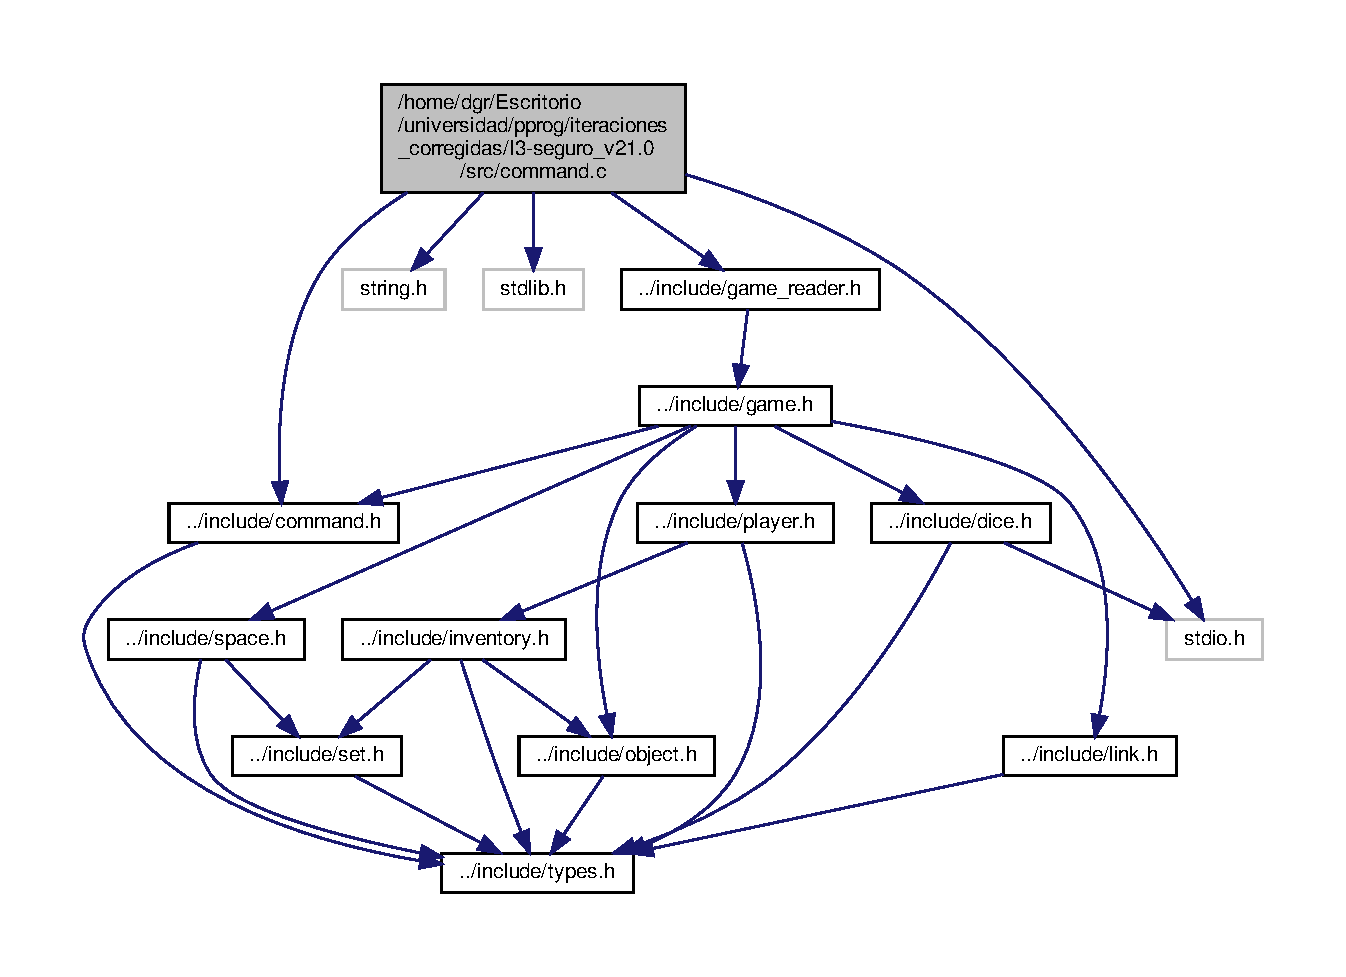
\includegraphics[width=350pt]{command_8c__incl}
\end{center}
\end{figure}
\subsection*{Data Structures}
\begin{DoxyCompactItemize}
\item 
struct \hyperlink{struct__Command}{\+\_\+\+Command}
\begin{DoxyCompactList}\small\item\em The command structure. \end{DoxyCompactList}\end{DoxyCompactItemize}
\subsection*{Functions}
\begin{DoxyCompactItemize}
\item 
\hyperlink{command_8h_a7d2935971c252377cb0fc1c8545dc2bc}{Command} $\ast$ \hyperlink{command_8c_a25a96480a40811cf60e301f6d050fee3}{command\+\_\+init} ()
\begin{DoxyCompactList}\small\item\em initialitates the structure command command\+\_\+init \end{DoxyCompactList}\item 
\hyperlink{command_8h_a7d2935971c252377cb0fc1c8545dc2bc}{Command} $\ast$ \hyperlink{command_8c_a3bb1dc14827ec48c5e358d02cd909bc5}{command\+\_\+get\+\_\+user\+\_\+input} (\hyperlink{command_8h_a7d2935971c252377cb0fc1c8545dc2bc}{Command} $\ast$cmd)
\begin{DoxyCompactList}\small\item\em get the principal command and the argument \end{DoxyCompactList}\item 
\hyperlink{command_8h_a0473597db8c45c0289b6b8e2f8abbe32}{T\+\_\+\+Command} \hyperlink{command_8c_ad35081cca7cf7ff3161e48beb3a34624}{command\+\_\+get\+\_\+principalcmd} (\hyperlink{command_8h_a7d2935971c252377cb0fc1c8545dc2bc}{Command} $\ast$cmd)
\begin{DoxyCompactList}\small\item\em get the command \end{DoxyCompactList}\item 
char $\ast$ \hyperlink{command_8c_a3392110efd7b39066a8aa5e6b4864ea8}{command\+\_\+get\+\_\+argument} (\hyperlink{command_8h_a7d2935971c252377cb0fc1c8545dc2bc}{Command} $\ast$cmd)
\begin{DoxyCompactList}\small\item\em get an argument \end{DoxyCompactList}\item 
\hyperlink{types_8h_a32c27cc471df37f4fc818d65de0a56c4}{S\+T\+A\+T\+US} \hyperlink{command_8c_a7df71b69fa875de1b55df0174545807b}{command\+\_\+destroy} (\hyperlink{command_8h_a7d2935971c252377cb0fc1c8545dc2bc}{Command} $\ast$cmd)
\begin{DoxyCompactList}\small\item\em free the strcture command \end{DoxyCompactList}\item 
\hyperlink{types_8h_a32c27cc471df37f4fc818d65de0a56c4}{S\+T\+A\+T\+US} \hyperlink{command_8c_ae06b30b8f869f7236ce1abe8b5167b8d}{command\+\_\+set\+\_\+principalcmd} (\hyperlink{command_8h_a7d2935971c252377cb0fc1c8545dc2bc}{Command} $\ast$cmd, \hyperlink{command_8h_a0473597db8c45c0289b6b8e2f8abbe32}{T\+\_\+\+Command} command)
\begin{DoxyCompactList}\small\item\em set an especific command \end{DoxyCompactList}\item 
\hyperlink{types_8h_a32c27cc471df37f4fc818d65de0a56c4}{S\+T\+A\+T\+US} \hyperlink{command_8c_a136c02c30eaf3dbaadcde50750ccafdc}{command\+\_\+set\+\_\+argument} (\hyperlink{command_8h_a7d2935971c252377cb0fc1c8545dc2bc}{Command} $\ast$cmd, char $\ast$argument)
\begin{DoxyCompactList}\small\item\em set an especific argument \end{DoxyCompactList}\item 
\hyperlink{types_8h_a32c27cc471df37f4fc818d65de0a56c4}{S\+T\+A\+T\+US} \hyperlink{command_8c_ab28a732878a02cf27db4fd57c6d68daa}{command\+\_\+set\+\_\+status} (\hyperlink{command_8h_a7d2935971c252377cb0fc1c8545dc2bc}{Command} $\ast$cmd, char $\ast$status)
\begin{DoxyCompactList}\small\item\em set an especific status \end{DoxyCompactList}\item 
char $\ast$ \hyperlink{command_8c_a228fde7cd02041d88322fd5c676f1302}{command\+\_\+get\+\_\+status} (\hyperlink{command_8h_a7d2935971c252377cb0fc1c8545dc2bc}{Command} $\ast$cmd)
\begin{DoxyCompactList}\small\item\em get an especific status \end{DoxyCompactList}\end{DoxyCompactItemize}
\subsection*{Variables}
\begin{DoxyCompactItemize}
\item 
char $\ast$ \hyperlink{command_8c_a464d0d851d33660f38485669bf66a8ac}{cmd\+\_\+to\+\_\+str} \mbox{[}\hyperlink{command_8h_ae180fe89f0ae48ce5c80ffaa18de9271}{N\+\_\+\+C\+MD}\mbox{]}\mbox{[}\hyperlink{command_8h_a8d93932dcdc527c13e06b688b68c7ffc}{N\+\_\+\+C\+M\+DT}\mbox{]} = \{\{\char`\"{}\char`\"{}, \char`\"{}no command\char`\"{}\}, \{\char`\"{}\char`\"{}, \char`\"{}unknown\char`\"{}\}, \{\char`\"{}e\char`\"{}, \char`\"{}exit\char`\"{}\}, \{\char`\"{}t\char`\"{}, \char`\"{}take\char`\"{}\}, \{\char`\"{}d\char`\"{}, \char`\"{}drop\char`\"{}\}, \{\char`\"{}rl\char`\"{}, \char`\"{}roll\char`\"{}\}, \{\char`\"{}m\char`\"{}, \char`\"{}move\char`\"{}\}, \{\char`\"{}i\char`\"{}, \char`\"{}inspect\char`\"{}\}, \{\char`\"{}n\char`\"{}, \char`\"{}next\char`\"{}\}, \{\char`\"{}b\char`\"{}, \char`\"{}back\char`\"{}\}, \{\char`\"{}r\char`\"{}, \char`\"{}right\char`\"{}\}, \{\char`\"{}l\char`\"{}, \char`\"{}left\char`\"{}\}\}
\begin{DoxyCompactList}\small\item\em matrix of commands \end{DoxyCompactList}\end{DoxyCompactItemize}


\subsection{Detailed Description}
It implements the command interpreter. 

\begin{DoxyAuthor}{Author}
Profesores P\+P\+R\+OG 
\end{DoxyAuthor}
\begin{DoxyVersion}{Version}
2.\+0 
\end{DoxyVersion}
\begin{DoxyDate}{Date}
13-\/01-\/2020 
\end{DoxyDate}
\begin{DoxyCopyright}{Copyright}
G\+NU Public License 
\end{DoxyCopyright}


\subsection{Function Documentation}
\mbox{\Hypertarget{command_8c_a7df71b69fa875de1b55df0174545807b}\label{command_8c_a7df71b69fa875de1b55df0174545807b}} 
\index{command.\+c@{command.\+c}!command\+\_\+destroy@{command\+\_\+destroy}}
\index{command\+\_\+destroy@{command\+\_\+destroy}!command.\+c@{command.\+c}}
\subsubsection{\texorpdfstring{command\+\_\+destroy()}{command\_destroy()}}
{\footnotesize\ttfamily \hyperlink{types_8h_a32c27cc471df37f4fc818d65de0a56c4}{S\+T\+A\+T\+US} command\+\_\+destroy (\begin{DoxyParamCaption}\item[{\hyperlink{command_8h_a7d2935971c252377cb0fc1c8545dc2bc}{Command} $\ast$}]{cmd }\end{DoxyParamCaption})}



free the strcture command 

command\+\_\+destroy

\begin{DoxyDate}{Date}
06-\/03-\/2019 
\end{DoxyDate}
\begin{DoxyAuthor}{Author}
José Manuel García Giráldez 
\end{DoxyAuthor}

\begin{DoxyParams}{Parameters}
{\em cmd} & the command structure \\
\hline
\end{DoxyParams}
\begin{DoxyReturn}{Returns}
E\+R\+R\+OR if there is an error, otherwise return OK 
\end{DoxyReturn}
\mbox{\Hypertarget{command_8c_a3392110efd7b39066a8aa5e6b4864ea8}\label{command_8c_a3392110efd7b39066a8aa5e6b4864ea8}} 
\index{command.\+c@{command.\+c}!command\+\_\+get\+\_\+argument@{command\+\_\+get\+\_\+argument}}
\index{command\+\_\+get\+\_\+argument@{command\+\_\+get\+\_\+argument}!command.\+c@{command.\+c}}
\subsubsection{\texorpdfstring{command\+\_\+get\+\_\+argument()}{command\_get\_argument()}}
{\footnotesize\ttfamily char$\ast$ command\+\_\+get\+\_\+argument (\begin{DoxyParamCaption}\item[{\hyperlink{command_8h_a7d2935971c252377cb0fc1c8545dc2bc}{Command} $\ast$}]{cmd }\end{DoxyParamCaption})}



get an argument 

command\+\_\+get\+\_\+argument

\begin{DoxyDate}{Date}
06-\/03-\/2019 
\end{DoxyDate}
\begin{DoxyAuthor}{Author}
José Manuel García Giráldez 
\end{DoxyAuthor}

\begin{DoxyParams}{Parameters}
{\em cmd} & the command structure \\
\hline
\end{DoxyParams}
\begin{DoxyReturn}{Returns}
the argument 
\end{DoxyReturn}
\mbox{\Hypertarget{command_8c_ad35081cca7cf7ff3161e48beb3a34624}\label{command_8c_ad35081cca7cf7ff3161e48beb3a34624}} 
\index{command.\+c@{command.\+c}!command\+\_\+get\+\_\+principalcmd@{command\+\_\+get\+\_\+principalcmd}}
\index{command\+\_\+get\+\_\+principalcmd@{command\+\_\+get\+\_\+principalcmd}!command.\+c@{command.\+c}}
\subsubsection{\texorpdfstring{command\+\_\+get\+\_\+principalcmd()}{command\_get\_principalcmd()}}
{\footnotesize\ttfamily \hyperlink{command_8h_a0473597db8c45c0289b6b8e2f8abbe32}{T\+\_\+\+Command} command\+\_\+get\+\_\+principalcmd (\begin{DoxyParamCaption}\item[{\hyperlink{command_8h_a7d2935971c252377cb0fc1c8545dc2bc}{Command} $\ast$}]{cmd }\end{DoxyParamCaption})}



get the command 

command\+\_\+get\+\_\+principalcmd

\begin{DoxyDate}{Date}
06-\/03-\/2019 
\end{DoxyDate}
\begin{DoxyAuthor}{Author}
José Manuel García Giráldez 
\end{DoxyAuthor}

\begin{DoxyParams}{Parameters}
{\em cmd} & the command structure \\
\hline
\end{DoxyParams}
\begin{DoxyReturn}{Returns}
the command 
\end{DoxyReturn}
\mbox{\Hypertarget{command_8c_a228fde7cd02041d88322fd5c676f1302}\label{command_8c_a228fde7cd02041d88322fd5c676f1302}} 
\index{command.\+c@{command.\+c}!command\+\_\+get\+\_\+status@{command\+\_\+get\+\_\+status}}
\index{command\+\_\+get\+\_\+status@{command\+\_\+get\+\_\+status}!command.\+c@{command.\+c}}
\subsubsection{\texorpdfstring{command\+\_\+get\+\_\+status()}{command\_get\_status()}}
{\footnotesize\ttfamily char$\ast$ command\+\_\+get\+\_\+status (\begin{DoxyParamCaption}\item[{\hyperlink{command_8h_a7d2935971c252377cb0fc1c8545dc2bc}{Command} $\ast$}]{cmd }\end{DoxyParamCaption})}



get an especific status 

command\+\_\+get\+\_\+status

\begin{DoxyDate}{Date}
06-\/03-\/2019 
\end{DoxyDate}
\begin{DoxyAuthor}{Author}
David Teófilo Garitagoitia Romero 
\end{DoxyAuthor}

\begin{DoxyParams}{Parameters}
{\em cmd} & the command structure \\
\hline
\end{DoxyParams}
\begin{DoxyReturn}{Returns}
N\+U\+LL if there is an error, otherwise return the status 
\end{DoxyReturn}
\mbox{\Hypertarget{command_8c_a3bb1dc14827ec48c5e358d02cd909bc5}\label{command_8c_a3bb1dc14827ec48c5e358d02cd909bc5}} 
\index{command.\+c@{command.\+c}!command\+\_\+get\+\_\+user\+\_\+input@{command\+\_\+get\+\_\+user\+\_\+input}}
\index{command\+\_\+get\+\_\+user\+\_\+input@{command\+\_\+get\+\_\+user\+\_\+input}!command.\+c@{command.\+c}}
\subsubsection{\texorpdfstring{command\+\_\+get\+\_\+user\+\_\+input()}{command\_get\_user\_input()}}
{\footnotesize\ttfamily \hyperlink{command_8h_a7d2935971c252377cb0fc1c8545dc2bc}{Command}$\ast$ command\+\_\+get\+\_\+user\+\_\+input (\begin{DoxyParamCaption}\item[{\hyperlink{command_8h_a7d2935971c252377cb0fc1c8545dc2bc}{Command} $\ast$}]{cmd }\end{DoxyParamCaption})}



get the principal command and the argument 

command\+\_\+get\+\_\+user\+\_\+input

\begin{DoxyDate}{Date}
06-\/03-\/2019 
\end{DoxyDate}
\begin{DoxyAuthor}{Author}
José Manuel García Giráldez 
\end{DoxyAuthor}

\begin{DoxyParams}{Parameters}
{\em cmd} & the command structure and file to log \\
\hline
\end{DoxyParams}
\begin{DoxyReturn}{Returns}
the structure command 
\end{DoxyReturn}
\mbox{\Hypertarget{command_8c_a25a96480a40811cf60e301f6d050fee3}\label{command_8c_a25a96480a40811cf60e301f6d050fee3}} 
\index{command.\+c@{command.\+c}!command\+\_\+init@{command\+\_\+init}}
\index{command\+\_\+init@{command\+\_\+init}!command.\+c@{command.\+c}}
\subsubsection{\texorpdfstring{command\+\_\+init()}{command\_init()}}
{\footnotesize\ttfamily \hyperlink{command_8h_a7d2935971c252377cb0fc1c8545dc2bc}{Command}$\ast$ command\+\_\+init (\begin{DoxyParamCaption}{ }\end{DoxyParamCaption})}



initialitates the structure command command\+\_\+init 

\begin{DoxyDate}{Date}
06-\/03-\/2019 
\end{DoxyDate}
\begin{DoxyAuthor}{Author}
José Manuel García Giráldez 
\end{DoxyAuthor}
\begin{DoxyReturn}{Returns}
the structure command 
\end{DoxyReturn}
\mbox{\Hypertarget{command_8c_a136c02c30eaf3dbaadcde50750ccafdc}\label{command_8c_a136c02c30eaf3dbaadcde50750ccafdc}} 
\index{command.\+c@{command.\+c}!command\+\_\+set\+\_\+argument@{command\+\_\+set\+\_\+argument}}
\index{command\+\_\+set\+\_\+argument@{command\+\_\+set\+\_\+argument}!command.\+c@{command.\+c}}
\subsubsection{\texorpdfstring{command\+\_\+set\+\_\+argument()}{command\_set\_argument()}}
{\footnotesize\ttfamily \hyperlink{types_8h_a32c27cc471df37f4fc818d65de0a56c4}{S\+T\+A\+T\+US} command\+\_\+set\+\_\+argument (\begin{DoxyParamCaption}\item[{\hyperlink{command_8h_a7d2935971c252377cb0fc1c8545dc2bc}{Command} $\ast$}]{cmd,  }\item[{char $\ast$}]{argument }\end{DoxyParamCaption})}



set an especific argument 

command\+\_\+set\+\_\+argument

\begin{DoxyDate}{Date}
06-\/03-\/2019 
\end{DoxyDate}
\begin{DoxyAuthor}{Author}
José Manuel García Giráldez 
\end{DoxyAuthor}

\begin{DoxyParams}{Parameters}
{\em cmd} & the command structure \\
\hline
{\em argument} & the argument we want to set \\
\hline
\end{DoxyParams}
\begin{DoxyReturn}{Returns}
E\+R\+R\+OR if there is an error, otherwise return OK 
\end{DoxyReturn}
\mbox{\Hypertarget{command_8c_ae06b30b8f869f7236ce1abe8b5167b8d}\label{command_8c_ae06b30b8f869f7236ce1abe8b5167b8d}} 
\index{command.\+c@{command.\+c}!command\+\_\+set\+\_\+principalcmd@{command\+\_\+set\+\_\+principalcmd}}
\index{command\+\_\+set\+\_\+principalcmd@{command\+\_\+set\+\_\+principalcmd}!command.\+c@{command.\+c}}
\subsubsection{\texorpdfstring{command\+\_\+set\+\_\+principalcmd()}{command\_set\_principalcmd()}}
{\footnotesize\ttfamily \hyperlink{types_8h_a32c27cc471df37f4fc818d65de0a56c4}{S\+T\+A\+T\+US} command\+\_\+set\+\_\+principalcmd (\begin{DoxyParamCaption}\item[{\hyperlink{command_8h_a7d2935971c252377cb0fc1c8545dc2bc}{Command} $\ast$}]{cmd,  }\item[{\hyperlink{command_8h_a0473597db8c45c0289b6b8e2f8abbe32}{T\+\_\+\+Command}}]{command }\end{DoxyParamCaption})}



set an especific command 

command\+\_\+set\+\_\+principalcmd

\begin{DoxyDate}{Date}
06-\/03-\/2019 
\end{DoxyDate}
\begin{DoxyAuthor}{Author}
José Manuel García Giráldez 
\end{DoxyAuthor}

\begin{DoxyParams}{Parameters}
{\em cmd} & the command structure \\
\hline
{\em command} & the command we want to set \\
\hline
\end{DoxyParams}
\begin{DoxyReturn}{Returns}
E\+R\+R\+OR if there is an error, otherwise return OK 
\end{DoxyReturn}
\mbox{\Hypertarget{command_8c_ab28a732878a02cf27db4fd57c6d68daa}\label{command_8c_ab28a732878a02cf27db4fd57c6d68daa}} 
\index{command.\+c@{command.\+c}!command\+\_\+set\+\_\+status@{command\+\_\+set\+\_\+status}}
\index{command\+\_\+set\+\_\+status@{command\+\_\+set\+\_\+status}!command.\+c@{command.\+c}}
\subsubsection{\texorpdfstring{command\+\_\+set\+\_\+status()}{command\_set\_status()}}
{\footnotesize\ttfamily \hyperlink{types_8h_a32c27cc471df37f4fc818d65de0a56c4}{S\+T\+A\+T\+US} command\+\_\+set\+\_\+status (\begin{DoxyParamCaption}\item[{\hyperlink{command_8h_a7d2935971c252377cb0fc1c8545dc2bc}{Command} $\ast$}]{cmd,  }\item[{char $\ast$}]{status }\end{DoxyParamCaption})}



set an especific status 

command\+\_\+set\+\_\+status

\begin{DoxyDate}{Date}
06-\/03-\/2019 
\end{DoxyDate}
\begin{DoxyAuthor}{Author}
David Teófilo Garitagoitia Romero 
\end{DoxyAuthor}

\begin{DoxyParams}{Parameters}
{\em cmd} & the command structure \\
\hline
{\em status} & the status we want to set \\
\hline
\end{DoxyParams}
\begin{DoxyReturn}{Returns}
E\+R\+R\+OR if there is an error, otherwise return OK 
\end{DoxyReturn}


\subsection{Variable Documentation}
\mbox{\Hypertarget{command_8c_a464d0d851d33660f38485669bf66a8ac}\label{command_8c_a464d0d851d33660f38485669bf66a8ac}} 
\index{command.\+c@{command.\+c}!cmd\+\_\+to\+\_\+str@{cmd\+\_\+to\+\_\+str}}
\index{cmd\+\_\+to\+\_\+str@{cmd\+\_\+to\+\_\+str}!command.\+c@{command.\+c}}
\subsubsection{\texorpdfstring{cmd\+\_\+to\+\_\+str}{cmd\_to\_str}}
{\footnotesize\ttfamily cmd\+\_\+to\+\_\+str = \{\{\char`\"{}\char`\"{}, \char`\"{}no command\char`\"{}\}, \{\char`\"{}\char`\"{}, \char`\"{}unknown\char`\"{}\}, \{\char`\"{}e\char`\"{}, \char`\"{}exit\char`\"{}\}, \{\char`\"{}t\char`\"{}, \char`\"{}take\char`\"{}\}, \{\char`\"{}d\char`\"{}, \char`\"{}drop\char`\"{}\}, \{\char`\"{}rl\char`\"{}, \char`\"{}roll\char`\"{}\}, \{\char`\"{}m\char`\"{}, \char`\"{}move\char`\"{}\}, \{\char`\"{}i\char`\"{}, \char`\"{}inspect\char`\"{}\}, \{\char`\"{}n\char`\"{}, \char`\"{}next\char`\"{}\}, \{\char`\"{}b\char`\"{}, \char`\"{}back\char`\"{}\}, \{\char`\"{}r\char`\"{}, \char`\"{}right\char`\"{}\}, \{\char`\"{}l\char`\"{}, \char`\"{}left\char`\"{}\}\}}



matrix of commands 

Details. 
\hypertarget{command__test_8c}{}\section{/home/dgr/\+Escritorio/universidad/pprog/iteraciones\+\_\+corregidas/\+I3-\/seguro\+\_\+v21.0/src/command\+\_\+test.c File Reference}
\label{command__test_8c}\index{/home/dgr/\+Escritorio/universidad/pprog/iteraciones\+\_\+corregidas/\+I3-\/seguro\+\_\+v21.\+0/src/command\+\_\+test.\+c@{/home/dgr/\+Escritorio/universidad/pprog/iteraciones\+\_\+corregidas/\+I3-\/seguro\+\_\+v21.\+0/src/command\+\_\+test.\+c}}


test to see if dice works correctly  


{\ttfamily \#include $<$stdio.\+h$>$}\newline
{\ttfamily \#include $<$string.\+h$>$}\newline
{\ttfamily \#include $<$stdlib.\+h$>$}\newline
{\ttfamily \#include \char`\"{}../include/test.\+h\char`\"{}}\newline
{\ttfamily \#include \char`\"{}../include/command.\+h\char`\"{}}\newline
{\ttfamily \#include \char`\"{}../include/command\+\_\+test.\+h\char`\"{}}\newline
{\ttfamily \#include \char`\"{}../include/types.\+h\char`\"{}}\newline
Include dependency graph for command\+\_\+test.\+c\+:
\nopagebreak
\begin{figure}[H]
\begin{center}
\leavevmode
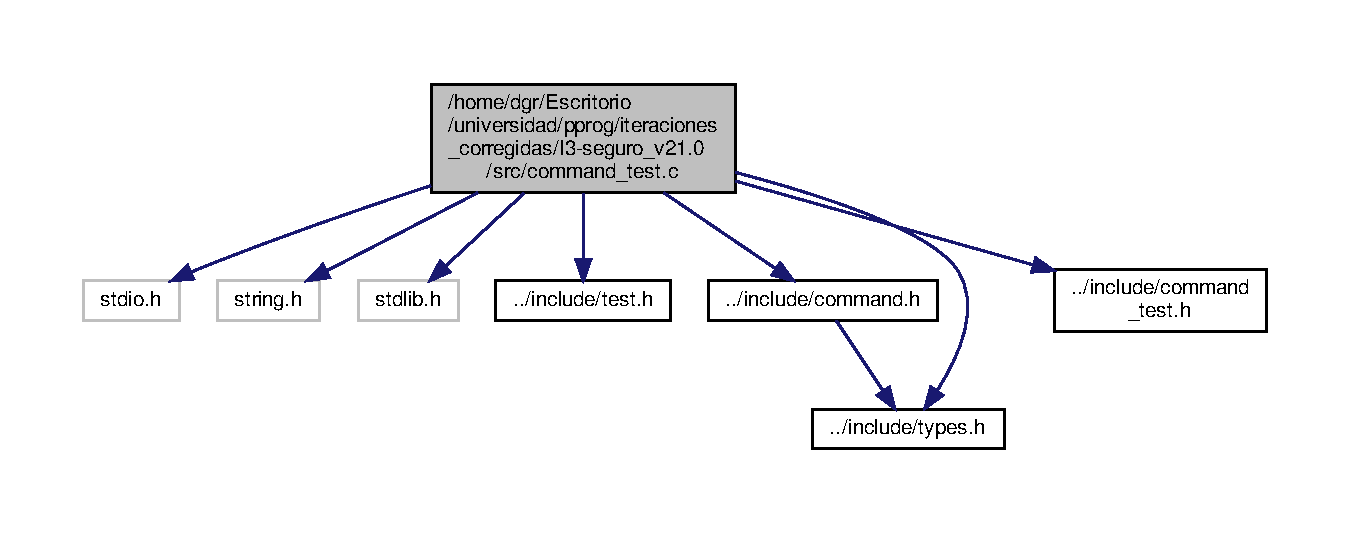
\includegraphics[width=350pt]{command__test_8c__incl}
\end{center}
\end{figure}
\subsection*{Macros}
\begin{DoxyCompactItemize}
\item 
\#define \hyperlink{command__test_8c_a2a77d2f2c5b698c69c19e1f8782bf709}{M\+A\+X\+\_\+\+T\+E\+S\+TS}~45
\begin{DoxyCompactList}\small\item\em maximum number of test \end{DoxyCompactList}\end{DoxyCompactItemize}
\subsection*{Functions}
\begin{DoxyCompactItemize}
\item 
int \hyperlink{command__test_8c_a3c04138a5bfe5d72780bb7e82a18e627}{main} (int argc, char $\ast$$\ast$argv)
\begin{DoxyCompactList}\small\item\em the main function of dice\+\_\+test main \end{DoxyCompactList}\item 
void \hyperlink{command__test_8c_af91aeb3bc73f994f5214b8954f3c4797}{test1\+\_\+command\+\_\+init} ()
\item 
void \hyperlink{command__test_8c_a084363877b09c47c4167fb675ba0a6c5}{test2\+\_\+command\+\_\+init} ()
\item 
void \hyperlink{command__test_8c_a1d44a3ed59cc78359d6c8c0d720347e1}{test3\+\_\+command\+\_\+init} ()
\item 
void \hyperlink{command__test_8c_a6367528b38336d716e765ea2d57f6d8c}{test4\+\_\+command\+\_\+init} ()
\item 
void \hyperlink{command__test_8c_a4e6817b2faaa57ed732eb9a68e671ef1}{test1\+\_\+command\+\_\+set\+\_\+principal\+\_\+cmd} ()
\item 
void \hyperlink{command__test_8c_a2f897a338775789b9e1b0b8a8647fd85}{test2\+\_\+command\+\_\+set\+\_\+principal\+\_\+cmd} ()
\item 
void \hyperlink{command__test_8c_a7e2613ae40c77091d31e9dd549c5d848}{test3\+\_\+command\+\_\+set\+\_\+principal\+\_\+cmd} ()
\item 
void \hyperlink{command__test_8c_a0485be612e6f281fe6e5b4dc778e2b72}{test4\+\_\+command\+\_\+set\+\_\+principal\+\_\+cmd} ()
\item 
void \hyperlink{command__test_8c_aa9706a5391086cfb6daf56613b55b351}{test5\+\_\+command\+\_\+set\+\_\+principal\+\_\+cmd} ()
\item 
void \hyperlink{command__test_8c_a1fd80f6afee487d3aa0386b22e85ac38}{test6\+\_\+command\+\_\+set\+\_\+principal\+\_\+cmd} ()
\item 
void \hyperlink{command__test_8c_aaacb4bcd77193d1e88615373040ea9a5}{test7\+\_\+command\+\_\+set\+\_\+principal\+\_\+cmd} ()
\item 
void \hyperlink{command__test_8c_a3c00c13f79566dca26966f011cdcb9b5}{test8\+\_\+command\+\_\+set\+\_\+principal\+\_\+cmd} ()
\item 
void \hyperlink{command__test_8c_af037a9eb46fd5e7700ec1f0760a5b9ec}{test9\+\_\+command\+\_\+set\+\_\+principal\+\_\+cmd} ()
\item 
void \hyperlink{command__test_8c_aba7be3a0f6ef3e6717088a21d32e9a21}{test10\+\_\+command\+\_\+set\+\_\+principal\+\_\+cmd} ()
\item 
void \hyperlink{command__test_8c_ae492f21ffdf46fc9380339f397f12675}{test11\+\_\+command\+\_\+set\+\_\+principal\+\_\+cmd} ()
\item 
void \hyperlink{command__test_8c_ab42210ac5001729f927be902384c51c6}{test12\+\_\+command\+\_\+set\+\_\+principal\+\_\+cmd} ()
\item 
void \hyperlink{command__test_8c_a86c724b0ce8b1a19b138fb1cb5dd84e3}{test1\+\_\+command\+\_\+set\+\_\+status} ()
\item 
void \hyperlink{command__test_8c_a67ea36686a450269ef95eace71e78867}{test2\+\_\+command\+\_\+set\+\_\+status} ()
\item 
void \hyperlink{command__test_8c_a5c554b37bf888c3077aa310982cedf14}{test3\+\_\+command\+\_\+set\+\_\+status} ()
\item 
void \hyperlink{command__test_8c_a88a8e8dddaca55194bd73c4d6796ec9b}{test1\+\_\+command\+\_\+set\+\_\+argument} ()
\item 
void \hyperlink{command__test_8c_a66f78c148ff91ffcbaa521f00d208a75}{test2\+\_\+command\+\_\+set\+\_\+argument} ()
\item 
void \hyperlink{command__test_8c_a69324b158668120d802451ce7c951d9e}{test3\+\_\+command\+\_\+set\+\_\+argument} ()
\item 
void \hyperlink{command__test_8c_aadf731a98e5122e70ede7cdc68ba621f}{test1\+\_\+command\+\_\+destroy} ()
\item 
void \hyperlink{command__test_8c_ad445f3e81035d4ab32ebc1526eb83fcb}{test2\+\_\+command\+\_\+destroy} ()
\item 
void \hyperlink{command__test_8c_a932afa8fb63c9b8ba551d030886ce491}{test1\+\_\+command\+\_\+get\+\_\+user\+\_\+input} ()
\item 
void \hyperlink{command__test_8c_a3ba7658db8aa069706b344d42ceabfaa}{test2\+\_\+command\+\_\+get\+\_\+user\+\_\+input} ()
\item 
void \hyperlink{command__test_8c_ae2d4b758fa9767317795c822b7334dec}{test3\+\_\+command\+\_\+get\+\_\+user\+\_\+input} ()
\item 
void \hyperlink{command__test_8c_a87e1a266b9beb6b31dd8e626694d5dd6}{test4\+\_\+command\+\_\+get\+\_\+user\+\_\+input} ()
\item 
void \hyperlink{command__test_8c_a3b7a4bfd103971720b0daef936b9251c}{test5\+\_\+command\+\_\+get\+\_\+user\+\_\+input} ()
\item 
void \hyperlink{command__test_8c_a85a9509e4435960ab89a0968666c2588}{test6\+\_\+command\+\_\+get\+\_\+user\+\_\+input} ()
\item 
void \hyperlink{command__test_8c_ab3a94f10959f43dca5f3a1254d2455a4}{test7\+\_\+command\+\_\+get\+\_\+user\+\_\+input} ()
\item 
void \hyperlink{command__test_8c_a96e8d3216af1419e01aaa68052a4ed26}{test8\+\_\+command\+\_\+get\+\_\+user\+\_\+input} ()
\item 
void \hyperlink{command__test_8c_ad9250b3696fed0b765bc703ecfa06066}{test9\+\_\+command\+\_\+get\+\_\+user\+\_\+input} ()
\item 
void \hyperlink{command__test_8c_a5a8b71fe0575431c76639d1a1703dd56}{test10\+\_\+command\+\_\+get\+\_\+user\+\_\+input} ()
\item 
void \hyperlink{command__test_8c_ada1f2861adf1a95726d5d08ecf6c015a}{test11\+\_\+command\+\_\+get\+\_\+user\+\_\+input} ()
\item 
void \hyperlink{command__test_8c_a01d0cd8d45e24b2b1a455a4ab50654cd}{test12\+\_\+command\+\_\+get\+\_\+user\+\_\+input} ()
\item 
void \hyperlink{command__test_8c_a274781536f1262b9c22ee97c1a57af18}{test13\+\_\+command\+\_\+get\+\_\+user\+\_\+input} ()
\item 
void \hyperlink{command__test_8c_a8f9bd7fc5112b6851b4e77a785984858}{test14\+\_\+command\+\_\+get\+\_\+user\+\_\+input} ()
\item 
void \hyperlink{command__test_8c_ae901b403f53f05148d2183d8205f968c}{test15\+\_\+command\+\_\+get\+\_\+user\+\_\+input} ()
\item 
void \hyperlink{command__test_8c_a9acb10b7ed10138a24190b90358e0583}{test16\+\_\+command\+\_\+get\+\_\+user\+\_\+input} ()
\item 
void \hyperlink{command__test_8c_a46ab7fb8f1c83596debe331b2c7bfbe0}{test17\+\_\+command\+\_\+get\+\_\+user\+\_\+input} ()
\item 
void \hyperlink{command__test_8c_a4db087cfa5bf22f248747b748745379f}{test18\+\_\+command\+\_\+get\+\_\+user\+\_\+input} ()
\item 
void \hyperlink{command__test_8c_a340bc65a10e7f7bdcddcef019bbd5aa7}{test19\+\_\+command\+\_\+get\+\_\+user\+\_\+input} ()
\item 
void \hyperlink{command__test_8c_a92cce7477f40656ebebe28d56142b528}{test20\+\_\+command\+\_\+get\+\_\+user\+\_\+input} ()
\item 
void \hyperlink{command__test_8c_aaf02a6c7423e84f000c00b8218a8a9a1}{test21\+\_\+command\+\_\+get\+\_\+user\+\_\+input} ()
\item 
void \hyperlink{command__test_8c_ac1ff85e1d54f46eccdbdaffec062d5c0}{test22\+\_\+command\+\_\+get\+\_\+user\+\_\+input} ()
\item 
void \hyperlink{command__test_8c_a618f500cde2987b4f746357b2a990b69}{test23\+\_\+command\+\_\+get\+\_\+user\+\_\+input} ()
\end{DoxyCompactItemize}


\subsection{Detailed Description}
test to see if dice works correctly 

\begin{DoxyAuthor}{Author}
David Teófilo Garitagoitia Romero 
\end{DoxyAuthor}
\begin{DoxyVersion}{Version}
2.\+0 
\end{DoxyVersion}
\begin{DoxyDate}{Date}
10-\/06-\/2020 
\end{DoxyDate}
\begin{DoxyCopyright}{Copyright}
G\+NU Public License 
\end{DoxyCopyright}


\subsection{Macro Definition Documentation}
\mbox{\Hypertarget{command__test_8c_a2a77d2f2c5b698c69c19e1f8782bf709}\label{command__test_8c_a2a77d2f2c5b698c69c19e1f8782bf709}} 
\index{command\+\_\+test.\+c@{command\+\_\+test.\+c}!M\+A\+X\+\_\+\+T\+E\+S\+TS@{M\+A\+X\+\_\+\+T\+E\+S\+TS}}
\index{M\+A\+X\+\_\+\+T\+E\+S\+TS@{M\+A\+X\+\_\+\+T\+E\+S\+TS}!command\+\_\+test.\+c@{command\+\_\+test.\+c}}
\subsubsection{\texorpdfstring{M\+A\+X\+\_\+\+T\+E\+S\+TS}{MAX\_TESTS}}
{\footnotesize\ttfamily \#define M\+A\+X\+\_\+\+T\+E\+S\+TS~45}



maximum number of test 

Details. 

\subsection{Function Documentation}
\mbox{\Hypertarget{command__test_8c_a3c04138a5bfe5d72780bb7e82a18e627}\label{command__test_8c_a3c04138a5bfe5d72780bb7e82a18e627}} 
\index{command\+\_\+test.\+c@{command\+\_\+test.\+c}!main@{main}}
\index{main@{main}!command\+\_\+test.\+c@{command\+\_\+test.\+c}}
\subsubsection{\texorpdfstring{main()}{main()}}
{\footnotesize\ttfamily int main (\begin{DoxyParamCaption}\item[{int}]{argc,  }\item[{char $\ast$$\ast$}]{argv }\end{DoxyParamCaption})}



the main function of dice\+\_\+test main 

\begin{DoxyDate}{Date}
10-\/06-\/2020 
\end{DoxyDate}
\begin{DoxyAuthor}{Author}
David Teófilo Garitagoitia Romero 
\end{DoxyAuthor}
\begin{DoxyReturn}{Returns}

\end{DoxyReturn}
\mbox{\Hypertarget{command__test_8c_a5a8b71fe0575431c76639d1a1703dd56}\label{command__test_8c_a5a8b71fe0575431c76639d1a1703dd56}} 
\index{command\+\_\+test.\+c@{command\+\_\+test.\+c}!test10\+\_\+command\+\_\+get\+\_\+user\+\_\+input@{test10\+\_\+command\+\_\+get\+\_\+user\+\_\+input}}
\index{test10\+\_\+command\+\_\+get\+\_\+user\+\_\+input@{test10\+\_\+command\+\_\+get\+\_\+user\+\_\+input}!command\+\_\+test.\+c@{command\+\_\+test.\+c}}
\subsubsection{\texorpdfstring{test10\+\_\+command\+\_\+get\+\_\+user\+\_\+input()}{test10\_command\_get\_user\_input()}}
{\footnotesize\ttfamily void test10\+\_\+command\+\_\+get\+\_\+user\+\_\+input (\begin{DoxyParamCaption}{ }\end{DoxyParamCaption})}

\begin{DoxyRefDesc}{Test}
\item[\hyperlink{test__test000034}{Test}]Test the command get user input function \end{DoxyRefDesc}
\begin{DoxyPrecond}{Precondition}
Use the text file with the instructions, in this case, the instruction is m n (move and the argument is n) 
\end{DoxyPrecond}
\begin{DoxyPostcond}{Postcondition}
The principal cmd must be move and the argument must be n 
\end{DoxyPostcond}
\mbox{\Hypertarget{command__test_8c_aba7be3a0f6ef3e6717088a21d32e9a21}\label{command__test_8c_aba7be3a0f6ef3e6717088a21d32e9a21}} 
\index{command\+\_\+test.\+c@{command\+\_\+test.\+c}!test10\+\_\+command\+\_\+set\+\_\+principal\+\_\+cmd@{test10\+\_\+command\+\_\+set\+\_\+principal\+\_\+cmd}}
\index{test10\+\_\+command\+\_\+set\+\_\+principal\+\_\+cmd@{test10\+\_\+command\+\_\+set\+\_\+principal\+\_\+cmd}!command\+\_\+test.\+c@{command\+\_\+test.\+c}}
\subsubsection{\texorpdfstring{test10\+\_\+command\+\_\+set\+\_\+principal\+\_\+cmd()}{test10\_command\_set\_principal\_cmd()}}
{\footnotesize\ttfamily void test10\+\_\+command\+\_\+set\+\_\+principal\+\_\+cmd (\begin{DoxyParamCaption}{ }\end{DoxyParamCaption})}

\begin{DoxyRefDesc}{Test}
\item[\hyperlink{test__test000014}{Test}]Test the command set principal cmd function \end{DoxyRefDesc}
\begin{DoxyPrecond}{Precondition}
An cmd as a parameter 
\end{DoxyPrecond}
\begin{DoxyPostcond}{Postcondition}
The principal cmd must be B\+A\+CK 
\end{DoxyPostcond}
\mbox{\Hypertarget{command__test_8c_ada1f2861adf1a95726d5d08ecf6c015a}\label{command__test_8c_ada1f2861adf1a95726d5d08ecf6c015a}} 
\index{command\+\_\+test.\+c@{command\+\_\+test.\+c}!test11\+\_\+command\+\_\+get\+\_\+user\+\_\+input@{test11\+\_\+command\+\_\+get\+\_\+user\+\_\+input}}
\index{test11\+\_\+command\+\_\+get\+\_\+user\+\_\+input@{test11\+\_\+command\+\_\+get\+\_\+user\+\_\+input}!command\+\_\+test.\+c@{command\+\_\+test.\+c}}
\subsubsection{\texorpdfstring{test11\+\_\+command\+\_\+get\+\_\+user\+\_\+input()}{test11\_command\_get\_user\_input()}}
{\footnotesize\ttfamily void test11\+\_\+command\+\_\+get\+\_\+user\+\_\+input (\begin{DoxyParamCaption}{ }\end{DoxyParamCaption})}

\begin{DoxyRefDesc}{Test}
\item[\hyperlink{test__test000035}{Test}]Test the command get user input function \end{DoxyRefDesc}
\begin{DoxyPrecond}{Precondition}
Use the text file with the instructions, in this case, the instruction is move south (move and the argument is south) 
\end{DoxyPrecond}
\begin{DoxyPostcond}{Postcondition}
The principal cmd must be move and the argument must be south 
\end{DoxyPostcond}
\mbox{\Hypertarget{command__test_8c_ae492f21ffdf46fc9380339f397f12675}\label{command__test_8c_ae492f21ffdf46fc9380339f397f12675}} 
\index{command\+\_\+test.\+c@{command\+\_\+test.\+c}!test11\+\_\+command\+\_\+set\+\_\+principal\+\_\+cmd@{test11\+\_\+command\+\_\+set\+\_\+principal\+\_\+cmd}}
\index{test11\+\_\+command\+\_\+set\+\_\+principal\+\_\+cmd@{test11\+\_\+command\+\_\+set\+\_\+principal\+\_\+cmd}!command\+\_\+test.\+c@{command\+\_\+test.\+c}}
\subsubsection{\texorpdfstring{test11\+\_\+command\+\_\+set\+\_\+principal\+\_\+cmd()}{test11\_command\_set\_principal\_cmd()}}
{\footnotesize\ttfamily void test11\+\_\+command\+\_\+set\+\_\+principal\+\_\+cmd (\begin{DoxyParamCaption}{ }\end{DoxyParamCaption})}

\begin{DoxyRefDesc}{Test}
\item[\hyperlink{test__test000015}{Test}]Test the command set principal cmd function \end{DoxyRefDesc}
\begin{DoxyPrecond}{Precondition}
An cmd as a parameter 
\end{DoxyPrecond}
\begin{DoxyPostcond}{Postcondition}
The principal cmd must be R\+I\+G\+HT 
\end{DoxyPostcond}
\mbox{\Hypertarget{command__test_8c_a01d0cd8d45e24b2b1a455a4ab50654cd}\label{command__test_8c_a01d0cd8d45e24b2b1a455a4ab50654cd}} 
\index{command\+\_\+test.\+c@{command\+\_\+test.\+c}!test12\+\_\+command\+\_\+get\+\_\+user\+\_\+input@{test12\+\_\+command\+\_\+get\+\_\+user\+\_\+input}}
\index{test12\+\_\+command\+\_\+get\+\_\+user\+\_\+input@{test12\+\_\+command\+\_\+get\+\_\+user\+\_\+input}!command\+\_\+test.\+c@{command\+\_\+test.\+c}}
\subsubsection{\texorpdfstring{test12\+\_\+command\+\_\+get\+\_\+user\+\_\+input()}{test12\_command\_get\_user\_input()}}
{\footnotesize\ttfamily void test12\+\_\+command\+\_\+get\+\_\+user\+\_\+input (\begin{DoxyParamCaption}{ }\end{DoxyParamCaption})}

\begin{DoxyRefDesc}{Test}
\item[\hyperlink{test__test000036}{Test}]Test the command get user input function \end{DoxyRefDesc}
\begin{DoxyPrecond}{Precondition}
Use the text file with the instructions, in this case, the instruction is n next (next) 
\end{DoxyPrecond}
\begin{DoxyPostcond}{Postcondition}
The principal cmd must be next and the argument must be \char`\"{}\textbackslash{}0\char`\"{} 
\end{DoxyPostcond}
\mbox{\Hypertarget{command__test_8c_ab42210ac5001729f927be902384c51c6}\label{command__test_8c_ab42210ac5001729f927be902384c51c6}} 
\index{command\+\_\+test.\+c@{command\+\_\+test.\+c}!test12\+\_\+command\+\_\+set\+\_\+principal\+\_\+cmd@{test12\+\_\+command\+\_\+set\+\_\+principal\+\_\+cmd}}
\index{test12\+\_\+command\+\_\+set\+\_\+principal\+\_\+cmd@{test12\+\_\+command\+\_\+set\+\_\+principal\+\_\+cmd}!command\+\_\+test.\+c@{command\+\_\+test.\+c}}
\subsubsection{\texorpdfstring{test12\+\_\+command\+\_\+set\+\_\+principal\+\_\+cmd()}{test12\_command\_set\_principal\_cmd()}}
{\footnotesize\ttfamily void test12\+\_\+command\+\_\+set\+\_\+principal\+\_\+cmd (\begin{DoxyParamCaption}{ }\end{DoxyParamCaption})}

\begin{DoxyRefDesc}{Test}
\item[\hyperlink{test__test000016}{Test}]Test the command set principal cmd function \end{DoxyRefDesc}
\begin{DoxyPrecond}{Precondition}
An cmd as a parameter 
\end{DoxyPrecond}
\begin{DoxyPostcond}{Postcondition}
The principal cmd must be L\+E\+FT 
\end{DoxyPostcond}
\mbox{\Hypertarget{command__test_8c_a274781536f1262b9c22ee97c1a57af18}\label{command__test_8c_a274781536f1262b9c22ee97c1a57af18}} 
\index{command\+\_\+test.\+c@{command\+\_\+test.\+c}!test13\+\_\+command\+\_\+get\+\_\+user\+\_\+input@{test13\+\_\+command\+\_\+get\+\_\+user\+\_\+input}}
\index{test13\+\_\+command\+\_\+get\+\_\+user\+\_\+input@{test13\+\_\+command\+\_\+get\+\_\+user\+\_\+input}!command\+\_\+test.\+c@{command\+\_\+test.\+c}}
\subsubsection{\texorpdfstring{test13\+\_\+command\+\_\+get\+\_\+user\+\_\+input()}{test13\_command\_get\_user\_input()}}
{\footnotesize\ttfamily void test13\+\_\+command\+\_\+get\+\_\+user\+\_\+input (\begin{DoxyParamCaption}{ }\end{DoxyParamCaption})}

\begin{DoxyRefDesc}{Test}
\item[\hyperlink{test__test000037}{Test}]Test the command get user input function \end{DoxyRefDesc}
\begin{DoxyPrecond}{Precondition}
Use the text file with the instructions, in this case, the instruction is next (next) 
\end{DoxyPrecond}
\begin{DoxyPostcond}{Postcondition}
The principal cmd must be next and the argument must be \char`\"{}\textbackslash{}0\char`\"{} 
\end{DoxyPostcond}
\mbox{\Hypertarget{command__test_8c_a8f9bd7fc5112b6851b4e77a785984858}\label{command__test_8c_a8f9bd7fc5112b6851b4e77a785984858}} 
\index{command\+\_\+test.\+c@{command\+\_\+test.\+c}!test14\+\_\+command\+\_\+get\+\_\+user\+\_\+input@{test14\+\_\+command\+\_\+get\+\_\+user\+\_\+input}}
\index{test14\+\_\+command\+\_\+get\+\_\+user\+\_\+input@{test14\+\_\+command\+\_\+get\+\_\+user\+\_\+input}!command\+\_\+test.\+c@{command\+\_\+test.\+c}}
\subsubsection{\texorpdfstring{test14\+\_\+command\+\_\+get\+\_\+user\+\_\+input()}{test14\_command\_get\_user\_input()}}
{\footnotesize\ttfamily void test14\+\_\+command\+\_\+get\+\_\+user\+\_\+input (\begin{DoxyParamCaption}{ }\end{DoxyParamCaption})}

\begin{DoxyRefDesc}{Test}
\item[\hyperlink{test__test000038}{Test}]Test the command get user input function \end{DoxyRefDesc}
\begin{DoxyPrecond}{Precondition}
Use the text file with the instructions, in this case, the instruction is b (back) 
\end{DoxyPrecond}
\begin{DoxyPostcond}{Postcondition}
The principal cmd must be back and the argument must be \char`\"{}\textbackslash{}0\char`\"{} 
\end{DoxyPostcond}
\mbox{\Hypertarget{command__test_8c_ae901b403f53f05148d2183d8205f968c}\label{command__test_8c_ae901b403f53f05148d2183d8205f968c}} 
\index{command\+\_\+test.\+c@{command\+\_\+test.\+c}!test15\+\_\+command\+\_\+get\+\_\+user\+\_\+input@{test15\+\_\+command\+\_\+get\+\_\+user\+\_\+input}}
\index{test15\+\_\+command\+\_\+get\+\_\+user\+\_\+input@{test15\+\_\+command\+\_\+get\+\_\+user\+\_\+input}!command\+\_\+test.\+c@{command\+\_\+test.\+c}}
\subsubsection{\texorpdfstring{test15\+\_\+command\+\_\+get\+\_\+user\+\_\+input()}{test15\_command\_get\_user\_input()}}
{\footnotesize\ttfamily void test15\+\_\+command\+\_\+get\+\_\+user\+\_\+input (\begin{DoxyParamCaption}{ }\end{DoxyParamCaption})}

\begin{DoxyRefDesc}{Test}
\item[\hyperlink{test__test000039}{Test}]Test the command get user input function \end{DoxyRefDesc}
\begin{DoxyPrecond}{Precondition}
Use the text file with the instructions, in this case, the instruction is back (back) 
\end{DoxyPrecond}
\begin{DoxyPostcond}{Postcondition}
The principal cmd must be back and the argument must be \char`\"{}\textbackslash{}0\char`\"{} 
\end{DoxyPostcond}
\mbox{\Hypertarget{command__test_8c_a9acb10b7ed10138a24190b90358e0583}\label{command__test_8c_a9acb10b7ed10138a24190b90358e0583}} 
\index{command\+\_\+test.\+c@{command\+\_\+test.\+c}!test16\+\_\+command\+\_\+get\+\_\+user\+\_\+input@{test16\+\_\+command\+\_\+get\+\_\+user\+\_\+input}}
\index{test16\+\_\+command\+\_\+get\+\_\+user\+\_\+input@{test16\+\_\+command\+\_\+get\+\_\+user\+\_\+input}!command\+\_\+test.\+c@{command\+\_\+test.\+c}}
\subsubsection{\texorpdfstring{test16\+\_\+command\+\_\+get\+\_\+user\+\_\+input()}{test16\_command\_get\_user\_input()}}
{\footnotesize\ttfamily void test16\+\_\+command\+\_\+get\+\_\+user\+\_\+input (\begin{DoxyParamCaption}{ }\end{DoxyParamCaption})}

\begin{DoxyRefDesc}{Test}
\item[\hyperlink{test__test000040}{Test}]Test the command get user input function \end{DoxyRefDesc}
\begin{DoxyPrecond}{Precondition}
Use the text file with the instructions, in this case, the instruction is r (right) 
\end{DoxyPrecond}
\begin{DoxyPostcond}{Postcondition}
The principal cmd must be right and the argument must be \char`\"{}\textbackslash{}0\char`\"{} 
\end{DoxyPostcond}
\mbox{\Hypertarget{command__test_8c_a46ab7fb8f1c83596debe331b2c7bfbe0}\label{command__test_8c_a46ab7fb8f1c83596debe331b2c7bfbe0}} 
\index{command\+\_\+test.\+c@{command\+\_\+test.\+c}!test17\+\_\+command\+\_\+get\+\_\+user\+\_\+input@{test17\+\_\+command\+\_\+get\+\_\+user\+\_\+input}}
\index{test17\+\_\+command\+\_\+get\+\_\+user\+\_\+input@{test17\+\_\+command\+\_\+get\+\_\+user\+\_\+input}!command\+\_\+test.\+c@{command\+\_\+test.\+c}}
\subsubsection{\texorpdfstring{test17\+\_\+command\+\_\+get\+\_\+user\+\_\+input()}{test17\_command\_get\_user\_input()}}
{\footnotesize\ttfamily void test17\+\_\+command\+\_\+get\+\_\+user\+\_\+input (\begin{DoxyParamCaption}{ }\end{DoxyParamCaption})}

\begin{DoxyRefDesc}{Test}
\item[\hyperlink{test__test000041}{Test}]Test the command get user input function \end{DoxyRefDesc}
\begin{DoxyPrecond}{Precondition}
Use the text file with the instructions, in this case, the instruction is right (right) 
\end{DoxyPrecond}
\begin{DoxyPostcond}{Postcondition}
The principal cmd must be right and the argument must be \char`\"{}\textbackslash{}0\char`\"{} 
\end{DoxyPostcond}
\mbox{\Hypertarget{command__test_8c_a4db087cfa5bf22f248747b748745379f}\label{command__test_8c_a4db087cfa5bf22f248747b748745379f}} 
\index{command\+\_\+test.\+c@{command\+\_\+test.\+c}!test18\+\_\+command\+\_\+get\+\_\+user\+\_\+input@{test18\+\_\+command\+\_\+get\+\_\+user\+\_\+input}}
\index{test18\+\_\+command\+\_\+get\+\_\+user\+\_\+input@{test18\+\_\+command\+\_\+get\+\_\+user\+\_\+input}!command\+\_\+test.\+c@{command\+\_\+test.\+c}}
\subsubsection{\texorpdfstring{test18\+\_\+command\+\_\+get\+\_\+user\+\_\+input()}{test18\_command\_get\_user\_input()}}
{\footnotesize\ttfamily void test18\+\_\+command\+\_\+get\+\_\+user\+\_\+input (\begin{DoxyParamCaption}{ }\end{DoxyParamCaption})}

\begin{DoxyRefDesc}{Test}
\item[\hyperlink{test__test000042}{Test}]Test the command get user input function \end{DoxyRefDesc}
\begin{DoxyPrecond}{Precondition}
Use the text file with the instructions, in this case, the instruction is l (left) 
\end{DoxyPrecond}
\begin{DoxyPostcond}{Postcondition}
The principal cmd must be left and the argument must be \char`\"{}\textbackslash{}0\char`\"{} 
\end{DoxyPostcond}
\mbox{\Hypertarget{command__test_8c_a340bc65a10e7f7bdcddcef019bbd5aa7}\label{command__test_8c_a340bc65a10e7f7bdcddcef019bbd5aa7}} 
\index{command\+\_\+test.\+c@{command\+\_\+test.\+c}!test19\+\_\+command\+\_\+get\+\_\+user\+\_\+input@{test19\+\_\+command\+\_\+get\+\_\+user\+\_\+input}}
\index{test19\+\_\+command\+\_\+get\+\_\+user\+\_\+input@{test19\+\_\+command\+\_\+get\+\_\+user\+\_\+input}!command\+\_\+test.\+c@{command\+\_\+test.\+c}}
\subsubsection{\texorpdfstring{test19\+\_\+command\+\_\+get\+\_\+user\+\_\+input()}{test19\_command\_get\_user\_input()}}
{\footnotesize\ttfamily void test19\+\_\+command\+\_\+get\+\_\+user\+\_\+input (\begin{DoxyParamCaption}{ }\end{DoxyParamCaption})}

\begin{DoxyRefDesc}{Test}
\item[\hyperlink{test__test000043}{Test}]Test the command get user input function \end{DoxyRefDesc}
\begin{DoxyPrecond}{Precondition}
Use the text file with the instructions, in this case, the instruction is left da igual (left) 
\end{DoxyPrecond}
\begin{DoxyPostcond}{Postcondition}
The principal cmd must be left and the argument must be \char`\"{}\textbackslash{}0\char`\"{} 
\end{DoxyPostcond}
\mbox{\Hypertarget{command__test_8c_aadf731a98e5122e70ede7cdc68ba621f}\label{command__test_8c_aadf731a98e5122e70ede7cdc68ba621f}} 
\index{command\+\_\+test.\+c@{command\+\_\+test.\+c}!test1\+\_\+command\+\_\+destroy@{test1\+\_\+command\+\_\+destroy}}
\index{test1\+\_\+command\+\_\+destroy@{test1\+\_\+command\+\_\+destroy}!command\+\_\+test.\+c@{command\+\_\+test.\+c}}
\subsubsection{\texorpdfstring{test1\+\_\+command\+\_\+destroy()}{test1\_command\_destroy()}}
{\footnotesize\ttfamily void test1\+\_\+command\+\_\+destroy (\begin{DoxyParamCaption}{ }\end{DoxyParamCaption})}

\begin{DoxyRefDesc}{Test}
\item[\hyperlink{test__test000023}{Test}]Test the command destroy function \end{DoxyRefDesc}
\begin{DoxyPrecond}{Precondition}
The cmd as a parameter 
\end{DoxyPrecond}
\begin{DoxyPostcond}{Postcondition}
No problems destroying the command 
\end{DoxyPostcond}
\mbox{\Hypertarget{command__test_8c_a932afa8fb63c9b8ba551d030886ce491}\label{command__test_8c_a932afa8fb63c9b8ba551d030886ce491}} 
\index{command\+\_\+test.\+c@{command\+\_\+test.\+c}!test1\+\_\+command\+\_\+get\+\_\+user\+\_\+input@{test1\+\_\+command\+\_\+get\+\_\+user\+\_\+input}}
\index{test1\+\_\+command\+\_\+get\+\_\+user\+\_\+input@{test1\+\_\+command\+\_\+get\+\_\+user\+\_\+input}!command\+\_\+test.\+c@{command\+\_\+test.\+c}}
\subsubsection{\texorpdfstring{test1\+\_\+command\+\_\+get\+\_\+user\+\_\+input()}{test1\_command\_get\_user\_input()}}
{\footnotesize\ttfamily void test1\+\_\+command\+\_\+get\+\_\+user\+\_\+input (\begin{DoxyParamCaption}{ }\end{DoxyParamCaption})}

\begin{DoxyRefDesc}{Test}
\item[\hyperlink{test__test000025}{Test}]Test the command get user input function \end{DoxyRefDesc}
\begin{DoxyPrecond}{Precondition}
Use the text file with the instructions, in this case, the instruction is \char`\"{}no se que estoy poniendo\char`\"{} (unknown command) 
\end{DoxyPrecond}
\begin{DoxyPostcond}{Postcondition}
The principal cmd must be unknow 
\end{DoxyPostcond}
\mbox{\Hypertarget{command__test_8c_af91aeb3bc73f994f5214b8954f3c4797}\label{command__test_8c_af91aeb3bc73f994f5214b8954f3c4797}} 
\index{command\+\_\+test.\+c@{command\+\_\+test.\+c}!test1\+\_\+command\+\_\+init@{test1\+\_\+command\+\_\+init}}
\index{test1\+\_\+command\+\_\+init@{test1\+\_\+command\+\_\+init}!command\+\_\+test.\+c@{command\+\_\+test.\+c}}
\subsubsection{\texorpdfstring{test1\+\_\+command\+\_\+init()}{test1\_command\_init()}}
{\footnotesize\ttfamily void test1\+\_\+command\+\_\+init (\begin{DoxyParamCaption}{ }\end{DoxyParamCaption})}

\begin{DoxyRefDesc}{Test}
\item[\hyperlink{test__test000001}{Test}]Test the command creation function \end{DoxyRefDesc}
\begin{DoxyPrecond}{Precondition}
An identifier as a parameter 
\end{DoxyPrecond}
\begin{DoxyPostcond}{Postcondition}
A non-\/null pointer to the created space 
\end{DoxyPostcond}
\mbox{\Hypertarget{command__test_8c_a88a8e8dddaca55194bd73c4d6796ec9b}\label{command__test_8c_a88a8e8dddaca55194bd73c4d6796ec9b}} 
\index{command\+\_\+test.\+c@{command\+\_\+test.\+c}!test1\+\_\+command\+\_\+set\+\_\+argument@{test1\+\_\+command\+\_\+set\+\_\+argument}}
\index{test1\+\_\+command\+\_\+set\+\_\+argument@{test1\+\_\+command\+\_\+set\+\_\+argument}!command\+\_\+test.\+c@{command\+\_\+test.\+c}}
\subsubsection{\texorpdfstring{test1\+\_\+command\+\_\+set\+\_\+argument()}{test1\_command\_set\_argument()}}
{\footnotesize\ttfamily void test1\+\_\+command\+\_\+set\+\_\+argument (\begin{DoxyParamCaption}{ }\end{DoxyParamCaption})}

\begin{DoxyRefDesc}{Test}
\item[\hyperlink{test__test000020}{Test}]Test the command set argument function \end{DoxyRefDesc}
\begin{DoxyPrecond}{Precondition}
An cmd as a parameter 
\end{DoxyPrecond}
\begin{DoxyPostcond}{Postcondition}
The argument of the cmd is argument 
\end{DoxyPostcond}
\mbox{\Hypertarget{command__test_8c_a4e6817b2faaa57ed732eb9a68e671ef1}\label{command__test_8c_a4e6817b2faaa57ed732eb9a68e671ef1}} 
\index{command\+\_\+test.\+c@{command\+\_\+test.\+c}!test1\+\_\+command\+\_\+set\+\_\+principal\+\_\+cmd@{test1\+\_\+command\+\_\+set\+\_\+principal\+\_\+cmd}}
\index{test1\+\_\+command\+\_\+set\+\_\+principal\+\_\+cmd@{test1\+\_\+command\+\_\+set\+\_\+principal\+\_\+cmd}!command\+\_\+test.\+c@{command\+\_\+test.\+c}}
\subsubsection{\texorpdfstring{test1\+\_\+command\+\_\+set\+\_\+principal\+\_\+cmd()}{test1\_command\_set\_principal\_cmd()}}
{\footnotesize\ttfamily void test1\+\_\+command\+\_\+set\+\_\+principal\+\_\+cmd (\begin{DoxyParamCaption}{ }\end{DoxyParamCaption})}

\begin{DoxyRefDesc}{Test}
\item[\hyperlink{test__test000005}{Test}]Test the command set principal cmd function \end{DoxyRefDesc}
\begin{DoxyPrecond}{Precondition}
An identifier as a parameter 
\end{DoxyPrecond}
\begin{DoxyPostcond}{Postcondition}
The principal cmd is the one entered 
\end{DoxyPostcond}
\mbox{\Hypertarget{command__test_8c_a86c724b0ce8b1a19b138fb1cb5dd84e3}\label{command__test_8c_a86c724b0ce8b1a19b138fb1cb5dd84e3}} 
\index{command\+\_\+test.\+c@{command\+\_\+test.\+c}!test1\+\_\+command\+\_\+set\+\_\+status@{test1\+\_\+command\+\_\+set\+\_\+status}}
\index{test1\+\_\+command\+\_\+set\+\_\+status@{test1\+\_\+command\+\_\+set\+\_\+status}!command\+\_\+test.\+c@{command\+\_\+test.\+c}}
\subsubsection{\texorpdfstring{test1\+\_\+command\+\_\+set\+\_\+status()}{test1\_command\_set\_status()}}
{\footnotesize\ttfamily void test1\+\_\+command\+\_\+set\+\_\+status (\begin{DoxyParamCaption}{ }\end{DoxyParamCaption})}

\begin{DoxyRefDesc}{Test}
\item[\hyperlink{test__test000017}{Test}]Test the command set status function \end{DoxyRefDesc}
\begin{DoxyPrecond}{Precondition}
An cmd as a parameter 
\end{DoxyPrecond}
\begin{DoxyPostcond}{Postcondition}
The status is OK 
\end{DoxyPostcond}
\mbox{\Hypertarget{command__test_8c_a92cce7477f40656ebebe28d56142b528}\label{command__test_8c_a92cce7477f40656ebebe28d56142b528}} 
\index{command\+\_\+test.\+c@{command\+\_\+test.\+c}!test20\+\_\+command\+\_\+get\+\_\+user\+\_\+input@{test20\+\_\+command\+\_\+get\+\_\+user\+\_\+input}}
\index{test20\+\_\+command\+\_\+get\+\_\+user\+\_\+input@{test20\+\_\+command\+\_\+get\+\_\+user\+\_\+input}!command\+\_\+test.\+c@{command\+\_\+test.\+c}}
\subsubsection{\texorpdfstring{test20\+\_\+command\+\_\+get\+\_\+user\+\_\+input()}{test20\_command\_get\_user\_input()}}
{\footnotesize\ttfamily void test20\+\_\+command\+\_\+get\+\_\+user\+\_\+input (\begin{DoxyParamCaption}{ }\end{DoxyParamCaption})}

\begin{DoxyRefDesc}{Test}
\item[\hyperlink{test__test000044}{Test}]Test the command get user input function \end{DoxyRefDesc}
\begin{DoxyPrecond}{Precondition}
Use the text file with the instructions, in this case, the instruction is rl (roll) 
\end{DoxyPrecond}
\begin{DoxyPostcond}{Postcondition}
The principal cmd must be roll and the argument must be \char`\"{}\textbackslash{}0\char`\"{} 
\end{DoxyPostcond}
\mbox{\Hypertarget{command__test_8c_aaf02a6c7423e84f000c00b8218a8a9a1}\label{command__test_8c_aaf02a6c7423e84f000c00b8218a8a9a1}} 
\index{command\+\_\+test.\+c@{command\+\_\+test.\+c}!test21\+\_\+command\+\_\+get\+\_\+user\+\_\+input@{test21\+\_\+command\+\_\+get\+\_\+user\+\_\+input}}
\index{test21\+\_\+command\+\_\+get\+\_\+user\+\_\+input@{test21\+\_\+command\+\_\+get\+\_\+user\+\_\+input}!command\+\_\+test.\+c@{command\+\_\+test.\+c}}
\subsubsection{\texorpdfstring{test21\+\_\+command\+\_\+get\+\_\+user\+\_\+input()}{test21\_command\_get\_user\_input()}}
{\footnotesize\ttfamily void test21\+\_\+command\+\_\+get\+\_\+user\+\_\+input (\begin{DoxyParamCaption}{ }\end{DoxyParamCaption})}

\begin{DoxyRefDesc}{Test}
\item[\hyperlink{test__test000045}{Test}]Test the command get user input function \end{DoxyRefDesc}
\begin{DoxyPrecond}{Precondition}
Use the text file with the instructions, in this case, the instruction is roll (roll) 
\end{DoxyPrecond}
\begin{DoxyPostcond}{Postcondition}
The principal cmd must be roll and the argument must be \char`\"{}\textbackslash{}0\char`\"{} 
\end{DoxyPostcond}
\mbox{\Hypertarget{command__test_8c_ac1ff85e1d54f46eccdbdaffec062d5c0}\label{command__test_8c_ac1ff85e1d54f46eccdbdaffec062d5c0}} 
\index{command\+\_\+test.\+c@{command\+\_\+test.\+c}!test22\+\_\+command\+\_\+get\+\_\+user\+\_\+input@{test22\+\_\+command\+\_\+get\+\_\+user\+\_\+input}}
\index{test22\+\_\+command\+\_\+get\+\_\+user\+\_\+input@{test22\+\_\+command\+\_\+get\+\_\+user\+\_\+input}!command\+\_\+test.\+c@{command\+\_\+test.\+c}}
\subsubsection{\texorpdfstring{test22\+\_\+command\+\_\+get\+\_\+user\+\_\+input()}{test22\_command\_get\_user\_input()}}
{\footnotesize\ttfamily void test22\+\_\+command\+\_\+get\+\_\+user\+\_\+input (\begin{DoxyParamCaption}{ }\end{DoxyParamCaption})}

\begin{DoxyRefDesc}{Test}
\item[\hyperlink{test__test000046}{Test}]Test the command get user input function \end{DoxyRefDesc}
\begin{DoxyPrecond}{Precondition}
Use the text file with the instructions, in this case, the instruction is d Pep (drop with Pep as argument) 
\end{DoxyPrecond}
\begin{DoxyPostcond}{Postcondition}
The principal cmd must be drop and the argument must be Pep 
\end{DoxyPostcond}
\mbox{\Hypertarget{command__test_8c_a618f500cde2987b4f746357b2a990b69}\label{command__test_8c_a618f500cde2987b4f746357b2a990b69}} 
\index{command\+\_\+test.\+c@{command\+\_\+test.\+c}!test23\+\_\+command\+\_\+get\+\_\+user\+\_\+input@{test23\+\_\+command\+\_\+get\+\_\+user\+\_\+input}}
\index{test23\+\_\+command\+\_\+get\+\_\+user\+\_\+input@{test23\+\_\+command\+\_\+get\+\_\+user\+\_\+input}!command\+\_\+test.\+c@{command\+\_\+test.\+c}}
\subsubsection{\texorpdfstring{test23\+\_\+command\+\_\+get\+\_\+user\+\_\+input()}{test23\_command\_get\_user\_input()}}
{\footnotesize\ttfamily void test23\+\_\+command\+\_\+get\+\_\+user\+\_\+input (\begin{DoxyParamCaption}{ }\end{DoxyParamCaption})}

\begin{DoxyRefDesc}{Test}
\item[\hyperlink{test__test000047}{Test}]Test the command get user input function \end{DoxyRefDesc}
\begin{DoxyPrecond}{Precondition}
Use the text file with the instructions, in this case, the instruction is drop Pep (drop with Pep as argument) 
\end{DoxyPrecond}
\begin{DoxyPostcond}{Postcondition}
The principal cmd must be drop and the argument must be Pep 
\end{DoxyPostcond}
\mbox{\Hypertarget{command__test_8c_ad445f3e81035d4ab32ebc1526eb83fcb}\label{command__test_8c_ad445f3e81035d4ab32ebc1526eb83fcb}} 
\index{command\+\_\+test.\+c@{command\+\_\+test.\+c}!test2\+\_\+command\+\_\+destroy@{test2\+\_\+command\+\_\+destroy}}
\index{test2\+\_\+command\+\_\+destroy@{test2\+\_\+command\+\_\+destroy}!command\+\_\+test.\+c@{command\+\_\+test.\+c}}
\subsubsection{\texorpdfstring{test2\+\_\+command\+\_\+destroy()}{test2\_command\_destroy()}}
{\footnotesize\ttfamily void test2\+\_\+command\+\_\+destroy (\begin{DoxyParamCaption}{ }\end{DoxyParamCaption})}

\begin{DoxyRefDesc}{Test}
\item[\hyperlink{test__test000024}{Test}]Test the command destroy function \end{DoxyRefDesc}
\begin{DoxyPrecond}{Precondition}
The cmd to destroy is a N\+U\+LL pointer 
\end{DoxyPrecond}
\begin{DoxyPostcond}{Postcondition}
It should be an E\+R\+R\+OR 
\end{DoxyPostcond}
\mbox{\Hypertarget{command__test_8c_a3ba7658db8aa069706b344d42ceabfaa}\label{command__test_8c_a3ba7658db8aa069706b344d42ceabfaa}} 
\index{command\+\_\+test.\+c@{command\+\_\+test.\+c}!test2\+\_\+command\+\_\+get\+\_\+user\+\_\+input@{test2\+\_\+command\+\_\+get\+\_\+user\+\_\+input}}
\index{test2\+\_\+command\+\_\+get\+\_\+user\+\_\+input@{test2\+\_\+command\+\_\+get\+\_\+user\+\_\+input}!command\+\_\+test.\+c@{command\+\_\+test.\+c}}
\subsubsection{\texorpdfstring{test2\+\_\+command\+\_\+get\+\_\+user\+\_\+input()}{test2\_command\_get\_user\_input()}}
{\footnotesize\ttfamily void test2\+\_\+command\+\_\+get\+\_\+user\+\_\+input (\begin{DoxyParamCaption}{ }\end{DoxyParamCaption})}

\begin{DoxyRefDesc}{Test}
\item[\hyperlink{test__test000026}{Test}]Test the command get user input function \end{DoxyRefDesc}
\begin{DoxyPrecond}{Precondition}
Use the text file with the instructions, in this case, the instruction is \char`\"{}\textbackslash{}n\char`\"{} (unknown) 
\end{DoxyPrecond}
\begin{DoxyPostcond}{Postcondition}
The argument must be \char`\"{}\textbackslash{}0\char`\"{} 
\end{DoxyPostcond}
\mbox{\Hypertarget{command__test_8c_a084363877b09c47c4167fb675ba0a6c5}\label{command__test_8c_a084363877b09c47c4167fb675ba0a6c5}} 
\index{command\+\_\+test.\+c@{command\+\_\+test.\+c}!test2\+\_\+command\+\_\+init@{test2\+\_\+command\+\_\+init}}
\index{test2\+\_\+command\+\_\+init@{test2\+\_\+command\+\_\+init}!command\+\_\+test.\+c@{command\+\_\+test.\+c}}
\subsubsection{\texorpdfstring{test2\+\_\+command\+\_\+init()}{test2\_command\_init()}}
{\footnotesize\ttfamily void test2\+\_\+command\+\_\+init (\begin{DoxyParamCaption}{ }\end{DoxyParamCaption})}

\begin{DoxyRefDesc}{Test}
\item[\hyperlink{test__test000002}{Test}]Test the command creation function \end{DoxyRefDesc}
\begin{DoxyPrecond}{Precondition}
An identifier as a parameter 
\end{DoxyPrecond}
\begin{DoxyPostcond}{Postcondition}
the argument must be \textquotesingle{}\textbackslash{}0\textquotesingle{} 
\end{DoxyPostcond}
\mbox{\Hypertarget{command__test_8c_a66f78c148ff91ffcbaa521f00d208a75}\label{command__test_8c_a66f78c148ff91ffcbaa521f00d208a75}} 
\index{command\+\_\+test.\+c@{command\+\_\+test.\+c}!test2\+\_\+command\+\_\+set\+\_\+argument@{test2\+\_\+command\+\_\+set\+\_\+argument}}
\index{test2\+\_\+command\+\_\+set\+\_\+argument@{test2\+\_\+command\+\_\+set\+\_\+argument}!command\+\_\+test.\+c@{command\+\_\+test.\+c}}
\subsubsection{\texorpdfstring{test2\+\_\+command\+\_\+set\+\_\+argument()}{test2\_command\_set\_argument()}}
{\footnotesize\ttfamily void test2\+\_\+command\+\_\+set\+\_\+argument (\begin{DoxyParamCaption}{ }\end{DoxyParamCaption})}

\begin{DoxyRefDesc}{Test}
\item[\hyperlink{test__test000021}{Test}]Test the command set argument function \end{DoxyRefDesc}
\begin{DoxyPrecond}{Precondition}
An cmd N\+U\+LL as a parameter 
\end{DoxyPrecond}
\begin{DoxyPostcond}{Postcondition}
It should be an E\+R\+R\+OR 
\end{DoxyPostcond}
\mbox{\Hypertarget{command__test_8c_a2f897a338775789b9e1b0b8a8647fd85}\label{command__test_8c_a2f897a338775789b9e1b0b8a8647fd85}} 
\index{command\+\_\+test.\+c@{command\+\_\+test.\+c}!test2\+\_\+command\+\_\+set\+\_\+principal\+\_\+cmd@{test2\+\_\+command\+\_\+set\+\_\+principal\+\_\+cmd}}
\index{test2\+\_\+command\+\_\+set\+\_\+principal\+\_\+cmd@{test2\+\_\+command\+\_\+set\+\_\+principal\+\_\+cmd}!command\+\_\+test.\+c@{command\+\_\+test.\+c}}
\subsubsection{\texorpdfstring{test2\+\_\+command\+\_\+set\+\_\+principal\+\_\+cmd()}{test2\_command\_set\_principal\_cmd()}}
{\footnotesize\ttfamily void test2\+\_\+command\+\_\+set\+\_\+principal\+\_\+cmd (\begin{DoxyParamCaption}{ }\end{DoxyParamCaption})}

\begin{DoxyRefDesc}{Test}
\item[\hyperlink{test__test000006}{Test}]Test the command set principal cmd function \end{DoxyRefDesc}
\begin{DoxyPrecond}{Precondition}
The command to set the principal cmd to is a pointer to N\+U\+LL 
\end{DoxyPrecond}
\begin{DoxyPostcond}{Postcondition}
The output must be E\+R\+R\+OR 
\end{DoxyPostcond}
\mbox{\Hypertarget{command__test_8c_a67ea36686a450269ef95eace71e78867}\label{command__test_8c_a67ea36686a450269ef95eace71e78867}} 
\index{command\+\_\+test.\+c@{command\+\_\+test.\+c}!test2\+\_\+command\+\_\+set\+\_\+status@{test2\+\_\+command\+\_\+set\+\_\+status}}
\index{test2\+\_\+command\+\_\+set\+\_\+status@{test2\+\_\+command\+\_\+set\+\_\+status}!command\+\_\+test.\+c@{command\+\_\+test.\+c}}
\subsubsection{\texorpdfstring{test2\+\_\+command\+\_\+set\+\_\+status()}{test2\_command\_set\_status()}}
{\footnotesize\ttfamily void test2\+\_\+command\+\_\+set\+\_\+status (\begin{DoxyParamCaption}{ }\end{DoxyParamCaption})}

\begin{DoxyRefDesc}{Test}
\item[\hyperlink{test__test000018}{Test}]Test the command set status function \end{DoxyRefDesc}
\begin{DoxyPrecond}{Precondition}
The cmd to set the status is N\+U\+LL 
\end{DoxyPrecond}
\begin{DoxyPostcond}{Postcondition}
It should return E\+R\+R\+OR 
\end{DoxyPostcond}
\mbox{\Hypertarget{command__test_8c_ae2d4b758fa9767317795c822b7334dec}\label{command__test_8c_ae2d4b758fa9767317795c822b7334dec}} 
\index{command\+\_\+test.\+c@{command\+\_\+test.\+c}!test3\+\_\+command\+\_\+get\+\_\+user\+\_\+input@{test3\+\_\+command\+\_\+get\+\_\+user\+\_\+input}}
\index{test3\+\_\+command\+\_\+get\+\_\+user\+\_\+input@{test3\+\_\+command\+\_\+get\+\_\+user\+\_\+input}!command\+\_\+test.\+c@{command\+\_\+test.\+c}}
\subsubsection{\texorpdfstring{test3\+\_\+command\+\_\+get\+\_\+user\+\_\+input()}{test3\_command\_get\_user\_input()}}
{\footnotesize\ttfamily void test3\+\_\+command\+\_\+get\+\_\+user\+\_\+input (\begin{DoxyParamCaption}{ }\end{DoxyParamCaption})}

\begin{DoxyRefDesc}{Test}
\item[\hyperlink{test__test000027}{Test}]Test the command get user input function \end{DoxyRefDesc}
\begin{DoxyPrecond}{Precondition}
Use the text file with the instructions, in this case, the instruction is e (exit) 
\end{DoxyPrecond}
\begin{DoxyPostcond}{Postcondition}
The principal cmd must be exit 
\end{DoxyPostcond}
\mbox{\Hypertarget{command__test_8c_a1d44a3ed59cc78359d6c8c0d720347e1}\label{command__test_8c_a1d44a3ed59cc78359d6c8c0d720347e1}} 
\index{command\+\_\+test.\+c@{command\+\_\+test.\+c}!test3\+\_\+command\+\_\+init@{test3\+\_\+command\+\_\+init}}
\index{test3\+\_\+command\+\_\+init@{test3\+\_\+command\+\_\+init}!command\+\_\+test.\+c@{command\+\_\+test.\+c}}
\subsubsection{\texorpdfstring{test3\+\_\+command\+\_\+init()}{test3\_command\_init()}}
{\footnotesize\ttfamily void test3\+\_\+command\+\_\+init (\begin{DoxyParamCaption}{ }\end{DoxyParamCaption})}

\begin{DoxyRefDesc}{Test}
\item[\hyperlink{test__test000003}{Test}]Test the command creation function \end{DoxyRefDesc}
\begin{DoxyPrecond}{Precondition}
An identifier as a parameter 
\end{DoxyPrecond}
\begin{DoxyPostcond}{Postcondition}
The status must ne E\+R\+R\+OR 
\end{DoxyPostcond}
\mbox{\Hypertarget{command__test_8c_a69324b158668120d802451ce7c951d9e}\label{command__test_8c_a69324b158668120d802451ce7c951d9e}} 
\index{command\+\_\+test.\+c@{command\+\_\+test.\+c}!test3\+\_\+command\+\_\+set\+\_\+argument@{test3\+\_\+command\+\_\+set\+\_\+argument}}
\index{test3\+\_\+command\+\_\+set\+\_\+argument@{test3\+\_\+command\+\_\+set\+\_\+argument}!command\+\_\+test.\+c@{command\+\_\+test.\+c}}
\subsubsection{\texorpdfstring{test3\+\_\+command\+\_\+set\+\_\+argument()}{test3\_command\_set\_argument()}}
{\footnotesize\ttfamily void test3\+\_\+command\+\_\+set\+\_\+argument (\begin{DoxyParamCaption}{ }\end{DoxyParamCaption})}

\begin{DoxyRefDesc}{Test}
\item[\hyperlink{test__test000022}{Test}]Test the command set argument function \end{DoxyRefDesc}
\begin{DoxyPrecond}{Precondition}
The argument is N\+U\+LL 
\end{DoxyPrecond}
\begin{DoxyPostcond}{Postcondition}
It should be an E\+R\+R\+OR 
\end{DoxyPostcond}
\mbox{\Hypertarget{command__test_8c_a7e2613ae40c77091d31e9dd549c5d848}\label{command__test_8c_a7e2613ae40c77091d31e9dd549c5d848}} 
\index{command\+\_\+test.\+c@{command\+\_\+test.\+c}!test3\+\_\+command\+\_\+set\+\_\+principal\+\_\+cmd@{test3\+\_\+command\+\_\+set\+\_\+principal\+\_\+cmd}}
\index{test3\+\_\+command\+\_\+set\+\_\+principal\+\_\+cmd@{test3\+\_\+command\+\_\+set\+\_\+principal\+\_\+cmd}!command\+\_\+test.\+c@{command\+\_\+test.\+c}}
\subsubsection{\texorpdfstring{test3\+\_\+command\+\_\+set\+\_\+principal\+\_\+cmd()}{test3\_command\_set\_principal\_cmd()}}
{\footnotesize\ttfamily void test3\+\_\+command\+\_\+set\+\_\+principal\+\_\+cmd (\begin{DoxyParamCaption}{ }\end{DoxyParamCaption})}

\begin{DoxyRefDesc}{Test}
\item[\hyperlink{test__test000007}{Test}]Test the command set principal cmd function \end{DoxyRefDesc}
\begin{DoxyPrecond}{Precondition}
An cmd as a parameter 
\end{DoxyPrecond}
\begin{DoxyPostcond}{Postcondition}
The principal cmd must be E\+X\+IT 
\end{DoxyPostcond}
\mbox{\Hypertarget{command__test_8c_a5c554b37bf888c3077aa310982cedf14}\label{command__test_8c_a5c554b37bf888c3077aa310982cedf14}} 
\index{command\+\_\+test.\+c@{command\+\_\+test.\+c}!test3\+\_\+command\+\_\+set\+\_\+status@{test3\+\_\+command\+\_\+set\+\_\+status}}
\index{test3\+\_\+command\+\_\+set\+\_\+status@{test3\+\_\+command\+\_\+set\+\_\+status}!command\+\_\+test.\+c@{command\+\_\+test.\+c}}
\subsubsection{\texorpdfstring{test3\+\_\+command\+\_\+set\+\_\+status()}{test3\_command\_set\_status()}}
{\footnotesize\ttfamily void test3\+\_\+command\+\_\+set\+\_\+status (\begin{DoxyParamCaption}{ }\end{DoxyParamCaption})}

\begin{DoxyRefDesc}{Test}
\item[\hyperlink{test__test000019}{Test}]Test the command set status function \end{DoxyRefDesc}
\begin{DoxyPrecond}{Precondition}
The status is N\+U\+LL 
\end{DoxyPrecond}
\begin{DoxyPostcond}{Postcondition}
It should return E\+R\+R\+OR 
\end{DoxyPostcond}
\mbox{\Hypertarget{command__test_8c_a87e1a266b9beb6b31dd8e626694d5dd6}\label{command__test_8c_a87e1a266b9beb6b31dd8e626694d5dd6}} 
\index{command\+\_\+test.\+c@{command\+\_\+test.\+c}!test4\+\_\+command\+\_\+get\+\_\+user\+\_\+input@{test4\+\_\+command\+\_\+get\+\_\+user\+\_\+input}}
\index{test4\+\_\+command\+\_\+get\+\_\+user\+\_\+input@{test4\+\_\+command\+\_\+get\+\_\+user\+\_\+input}!command\+\_\+test.\+c@{command\+\_\+test.\+c}}
\subsubsection{\texorpdfstring{test4\+\_\+command\+\_\+get\+\_\+user\+\_\+input()}{test4\_command\_get\_user\_input()}}
{\footnotesize\ttfamily void test4\+\_\+command\+\_\+get\+\_\+user\+\_\+input (\begin{DoxyParamCaption}{ }\end{DoxyParamCaption})}

\begin{DoxyRefDesc}{Test}
\item[\hyperlink{test__test000028}{Test}]Test the command get user input function \end{DoxyRefDesc}
\begin{DoxyPrecond}{Precondition}
Use the text file with the instructions, in this case, the instruction is e (exit) 
\end{DoxyPrecond}
\begin{DoxyPostcond}{Postcondition}
The principal cmd must be exit 
\end{DoxyPostcond}
\mbox{\Hypertarget{command__test_8c_a6367528b38336d716e765ea2d57f6d8c}\label{command__test_8c_a6367528b38336d716e765ea2d57f6d8c}} 
\index{command\+\_\+test.\+c@{command\+\_\+test.\+c}!test4\+\_\+command\+\_\+init@{test4\+\_\+command\+\_\+init}}
\index{test4\+\_\+command\+\_\+init@{test4\+\_\+command\+\_\+init}!command\+\_\+test.\+c@{command\+\_\+test.\+c}}
\subsubsection{\texorpdfstring{test4\+\_\+command\+\_\+init()}{test4\_command\_init()}}
{\footnotesize\ttfamily void test4\+\_\+command\+\_\+init (\begin{DoxyParamCaption}{ }\end{DoxyParamCaption})}

\begin{DoxyRefDesc}{Test}
\item[\hyperlink{test__test000004}{Test}]Test the command creation function \end{DoxyRefDesc}
\begin{DoxyPrecond}{Precondition}
An identifier as a parameter 
\end{DoxyPrecond}
\begin{DoxyPostcond}{Postcondition}
The principal cmd must be N\+O\+\_\+\+C\+MD 
\end{DoxyPostcond}
\mbox{\Hypertarget{command__test_8c_a0485be612e6f281fe6e5b4dc778e2b72}\label{command__test_8c_a0485be612e6f281fe6e5b4dc778e2b72}} 
\index{command\+\_\+test.\+c@{command\+\_\+test.\+c}!test4\+\_\+command\+\_\+set\+\_\+principal\+\_\+cmd@{test4\+\_\+command\+\_\+set\+\_\+principal\+\_\+cmd}}
\index{test4\+\_\+command\+\_\+set\+\_\+principal\+\_\+cmd@{test4\+\_\+command\+\_\+set\+\_\+principal\+\_\+cmd}!command\+\_\+test.\+c@{command\+\_\+test.\+c}}
\subsubsection{\texorpdfstring{test4\+\_\+command\+\_\+set\+\_\+principal\+\_\+cmd()}{test4\_command\_set\_principal\_cmd()}}
{\footnotesize\ttfamily void test4\+\_\+command\+\_\+set\+\_\+principal\+\_\+cmd (\begin{DoxyParamCaption}{ }\end{DoxyParamCaption})}

\begin{DoxyRefDesc}{Test}
\item[\hyperlink{test__test000008}{Test}]Test the command set principal cmd function \end{DoxyRefDesc}
\begin{DoxyPrecond}{Precondition}
An cmd as a parameter 
\end{DoxyPrecond}
\begin{DoxyPostcond}{Postcondition}
The principal cmd must be T\+A\+KE 
\end{DoxyPostcond}
\mbox{\Hypertarget{command__test_8c_a3b7a4bfd103971720b0daef936b9251c}\label{command__test_8c_a3b7a4bfd103971720b0daef936b9251c}} 
\index{command\+\_\+test.\+c@{command\+\_\+test.\+c}!test5\+\_\+command\+\_\+get\+\_\+user\+\_\+input@{test5\+\_\+command\+\_\+get\+\_\+user\+\_\+input}}
\index{test5\+\_\+command\+\_\+get\+\_\+user\+\_\+input@{test5\+\_\+command\+\_\+get\+\_\+user\+\_\+input}!command\+\_\+test.\+c@{command\+\_\+test.\+c}}
\subsubsection{\texorpdfstring{test5\+\_\+command\+\_\+get\+\_\+user\+\_\+input()}{test5\_command\_get\_user\_input()}}
{\footnotesize\ttfamily void test5\+\_\+command\+\_\+get\+\_\+user\+\_\+input (\begin{DoxyParamCaption}{ }\end{DoxyParamCaption})}

\begin{DoxyRefDesc}{Test}
\item[\hyperlink{test__test000029}{Test}]Test the command get user input function \end{DoxyRefDesc}
\begin{DoxyPrecond}{Precondition}
Use the text file with the instructions, in this case, the instruction is t (take without argument) 
\end{DoxyPrecond}
\begin{DoxyPostcond}{Postcondition}
The argument should be \char`\"{}\textbackslash{}0\char`\"{} 
\end{DoxyPostcond}
\mbox{\Hypertarget{command__test_8c_aa9706a5391086cfb6daf56613b55b351}\label{command__test_8c_aa9706a5391086cfb6daf56613b55b351}} 
\index{command\+\_\+test.\+c@{command\+\_\+test.\+c}!test5\+\_\+command\+\_\+set\+\_\+principal\+\_\+cmd@{test5\+\_\+command\+\_\+set\+\_\+principal\+\_\+cmd}}
\index{test5\+\_\+command\+\_\+set\+\_\+principal\+\_\+cmd@{test5\+\_\+command\+\_\+set\+\_\+principal\+\_\+cmd}!command\+\_\+test.\+c@{command\+\_\+test.\+c}}
\subsubsection{\texorpdfstring{test5\+\_\+command\+\_\+set\+\_\+principal\+\_\+cmd()}{test5\_command\_set\_principal\_cmd()}}
{\footnotesize\ttfamily void test5\+\_\+command\+\_\+set\+\_\+principal\+\_\+cmd (\begin{DoxyParamCaption}{ }\end{DoxyParamCaption})}

\begin{DoxyRefDesc}{Test}
\item[\hyperlink{test__test000009}{Test}]Test the command set principal cmd function \end{DoxyRefDesc}
\begin{DoxyPrecond}{Precondition}
An cmd as a parameter 
\end{DoxyPrecond}
\begin{DoxyPostcond}{Postcondition}
The principal cmd must be D\+R\+OP 
\end{DoxyPostcond}
\mbox{\Hypertarget{command__test_8c_a85a9509e4435960ab89a0968666c2588}\label{command__test_8c_a85a9509e4435960ab89a0968666c2588}} 
\index{command\+\_\+test.\+c@{command\+\_\+test.\+c}!test6\+\_\+command\+\_\+get\+\_\+user\+\_\+input@{test6\+\_\+command\+\_\+get\+\_\+user\+\_\+input}}
\index{test6\+\_\+command\+\_\+get\+\_\+user\+\_\+input@{test6\+\_\+command\+\_\+get\+\_\+user\+\_\+input}!command\+\_\+test.\+c@{command\+\_\+test.\+c}}
\subsubsection{\texorpdfstring{test6\+\_\+command\+\_\+get\+\_\+user\+\_\+input()}{test6\_command\_get\_user\_input()}}
{\footnotesize\ttfamily void test6\+\_\+command\+\_\+get\+\_\+user\+\_\+input (\begin{DoxyParamCaption}{ }\end{DoxyParamCaption})}

\begin{DoxyRefDesc}{Test}
\item[\hyperlink{test__test000030}{Test}]Test the command get user input function \end{DoxyRefDesc}
\begin{DoxyPrecond}{Precondition}
Use the text file with the instructions, in this case, the instruction is take 2 (take and the argument is 2) 
\end{DoxyPrecond}
\begin{DoxyPostcond}{Postcondition}
The principal cmd must be take 
\end{DoxyPostcond}
\mbox{\Hypertarget{command__test_8c_a1fd80f6afee487d3aa0386b22e85ac38}\label{command__test_8c_a1fd80f6afee487d3aa0386b22e85ac38}} 
\index{command\+\_\+test.\+c@{command\+\_\+test.\+c}!test6\+\_\+command\+\_\+set\+\_\+principal\+\_\+cmd@{test6\+\_\+command\+\_\+set\+\_\+principal\+\_\+cmd}}
\index{test6\+\_\+command\+\_\+set\+\_\+principal\+\_\+cmd@{test6\+\_\+command\+\_\+set\+\_\+principal\+\_\+cmd}!command\+\_\+test.\+c@{command\+\_\+test.\+c}}
\subsubsection{\texorpdfstring{test6\+\_\+command\+\_\+set\+\_\+principal\+\_\+cmd()}{test6\_command\_set\_principal\_cmd()}}
{\footnotesize\ttfamily void test6\+\_\+command\+\_\+set\+\_\+principal\+\_\+cmd (\begin{DoxyParamCaption}{ }\end{DoxyParamCaption})}

\begin{DoxyRefDesc}{Test}
\item[\hyperlink{test__test000010}{Test}]Test the command set principal cmd function \end{DoxyRefDesc}
\begin{DoxyPrecond}{Precondition}
An cmd as a parameter 
\end{DoxyPrecond}
\begin{DoxyPostcond}{Postcondition}
The principal cmd must be R\+O\+LL 
\end{DoxyPostcond}
\mbox{\Hypertarget{command__test_8c_ab3a94f10959f43dca5f3a1254d2455a4}\label{command__test_8c_ab3a94f10959f43dca5f3a1254d2455a4}} 
\index{command\+\_\+test.\+c@{command\+\_\+test.\+c}!test7\+\_\+command\+\_\+get\+\_\+user\+\_\+input@{test7\+\_\+command\+\_\+get\+\_\+user\+\_\+input}}
\index{test7\+\_\+command\+\_\+get\+\_\+user\+\_\+input@{test7\+\_\+command\+\_\+get\+\_\+user\+\_\+input}!command\+\_\+test.\+c@{command\+\_\+test.\+c}}
\subsubsection{\texorpdfstring{test7\+\_\+command\+\_\+get\+\_\+user\+\_\+input()}{test7\_command\_get\_user\_input()}}
{\footnotesize\ttfamily void test7\+\_\+command\+\_\+get\+\_\+user\+\_\+input (\begin{DoxyParamCaption}{ }\end{DoxyParamCaption})}

\begin{DoxyRefDesc}{Test}
\item[\hyperlink{test__test000031}{Test}]Test the command get user input function \end{DoxyRefDesc}
\begin{DoxyPrecond}{Precondition}
Use the text file with the instructions, in this case, the instruction is take 2 (take and the argument is 2) 
\end{DoxyPrecond}
\begin{DoxyPostcond}{Postcondition}
The principal cmd must be take and the argument must be 2 
\end{DoxyPostcond}
\mbox{\Hypertarget{command__test_8c_aaacb4bcd77193d1e88615373040ea9a5}\label{command__test_8c_aaacb4bcd77193d1e88615373040ea9a5}} 
\index{command\+\_\+test.\+c@{command\+\_\+test.\+c}!test7\+\_\+command\+\_\+set\+\_\+principal\+\_\+cmd@{test7\+\_\+command\+\_\+set\+\_\+principal\+\_\+cmd}}
\index{test7\+\_\+command\+\_\+set\+\_\+principal\+\_\+cmd@{test7\+\_\+command\+\_\+set\+\_\+principal\+\_\+cmd}!command\+\_\+test.\+c@{command\+\_\+test.\+c}}
\subsubsection{\texorpdfstring{test7\+\_\+command\+\_\+set\+\_\+principal\+\_\+cmd()}{test7\_command\_set\_principal\_cmd()}}
{\footnotesize\ttfamily void test7\+\_\+command\+\_\+set\+\_\+principal\+\_\+cmd (\begin{DoxyParamCaption}{ }\end{DoxyParamCaption})}

\begin{DoxyRefDesc}{Test}
\item[\hyperlink{test__test000011}{Test}]Test the command set principal cmd function \end{DoxyRefDesc}
\begin{DoxyPrecond}{Precondition}
An cmd as a parameter 
\end{DoxyPrecond}
\begin{DoxyPostcond}{Postcondition}
The principal cmd must be M\+O\+VE 
\end{DoxyPostcond}
\mbox{\Hypertarget{command__test_8c_a96e8d3216af1419e01aaa68052a4ed26}\label{command__test_8c_a96e8d3216af1419e01aaa68052a4ed26}} 
\index{command\+\_\+test.\+c@{command\+\_\+test.\+c}!test8\+\_\+command\+\_\+get\+\_\+user\+\_\+input@{test8\+\_\+command\+\_\+get\+\_\+user\+\_\+input}}
\index{test8\+\_\+command\+\_\+get\+\_\+user\+\_\+input@{test8\+\_\+command\+\_\+get\+\_\+user\+\_\+input}!command\+\_\+test.\+c@{command\+\_\+test.\+c}}
\subsubsection{\texorpdfstring{test8\+\_\+command\+\_\+get\+\_\+user\+\_\+input()}{test8\_command\_get\_user\_input()}}
{\footnotesize\ttfamily void test8\+\_\+command\+\_\+get\+\_\+user\+\_\+input (\begin{DoxyParamCaption}{ }\end{DoxyParamCaption})}

\begin{DoxyRefDesc}{Test}
\item[\hyperlink{test__test000032}{Test}]Test the command get user input function \end{DoxyRefDesc}
\begin{DoxyPrecond}{Precondition}
Use the text file with the instructions, in this case, the instruction is i space (inspect and the argument is space) 
\end{DoxyPrecond}
\begin{DoxyPostcond}{Postcondition}
The principal cmd must be inspect and the argument must be space 
\end{DoxyPostcond}
\mbox{\Hypertarget{command__test_8c_a3c00c13f79566dca26966f011cdcb9b5}\label{command__test_8c_a3c00c13f79566dca26966f011cdcb9b5}} 
\index{command\+\_\+test.\+c@{command\+\_\+test.\+c}!test8\+\_\+command\+\_\+set\+\_\+principal\+\_\+cmd@{test8\+\_\+command\+\_\+set\+\_\+principal\+\_\+cmd}}
\index{test8\+\_\+command\+\_\+set\+\_\+principal\+\_\+cmd@{test8\+\_\+command\+\_\+set\+\_\+principal\+\_\+cmd}!command\+\_\+test.\+c@{command\+\_\+test.\+c}}
\subsubsection{\texorpdfstring{test8\+\_\+command\+\_\+set\+\_\+principal\+\_\+cmd()}{test8\_command\_set\_principal\_cmd()}}
{\footnotesize\ttfamily void test8\+\_\+command\+\_\+set\+\_\+principal\+\_\+cmd (\begin{DoxyParamCaption}{ }\end{DoxyParamCaption})}

\begin{DoxyRefDesc}{Test}
\item[\hyperlink{test__test000012}{Test}]Test the command set principal cmd function \end{DoxyRefDesc}
\begin{DoxyPrecond}{Precondition}
An cmd as a parameter 
\end{DoxyPrecond}
\begin{DoxyPostcond}{Postcondition}
The principal cmd must be I\+N\+S\+P\+E\+CT 
\end{DoxyPostcond}
\mbox{\Hypertarget{command__test_8c_ad9250b3696fed0b765bc703ecfa06066}\label{command__test_8c_ad9250b3696fed0b765bc703ecfa06066}} 
\index{command\+\_\+test.\+c@{command\+\_\+test.\+c}!test9\+\_\+command\+\_\+get\+\_\+user\+\_\+input@{test9\+\_\+command\+\_\+get\+\_\+user\+\_\+input}}
\index{test9\+\_\+command\+\_\+get\+\_\+user\+\_\+input@{test9\+\_\+command\+\_\+get\+\_\+user\+\_\+input}!command\+\_\+test.\+c@{command\+\_\+test.\+c}}
\subsubsection{\texorpdfstring{test9\+\_\+command\+\_\+get\+\_\+user\+\_\+input()}{test9\_command\_get\_user\_input()}}
{\footnotesize\ttfamily void test9\+\_\+command\+\_\+get\+\_\+user\+\_\+input (\begin{DoxyParamCaption}{ }\end{DoxyParamCaption})}

\begin{DoxyRefDesc}{Test}
\item[\hyperlink{test__test000033}{Test}]Test the command get user input function \end{DoxyRefDesc}
\begin{DoxyPrecond}{Precondition}
Use the text file with the instructions, in this case, the instruction is inspect object (inspect and the argument is object) 
\end{DoxyPrecond}
\begin{DoxyPostcond}{Postcondition}
The principal cmd must be inspect and the argument must be object 
\end{DoxyPostcond}
\mbox{\Hypertarget{command__test_8c_af037a9eb46fd5e7700ec1f0760a5b9ec}\label{command__test_8c_af037a9eb46fd5e7700ec1f0760a5b9ec}} 
\index{command\+\_\+test.\+c@{command\+\_\+test.\+c}!test9\+\_\+command\+\_\+set\+\_\+principal\+\_\+cmd@{test9\+\_\+command\+\_\+set\+\_\+principal\+\_\+cmd}}
\index{test9\+\_\+command\+\_\+set\+\_\+principal\+\_\+cmd@{test9\+\_\+command\+\_\+set\+\_\+principal\+\_\+cmd}!command\+\_\+test.\+c@{command\+\_\+test.\+c}}
\subsubsection{\texorpdfstring{test9\+\_\+command\+\_\+set\+\_\+principal\+\_\+cmd()}{test9\_command\_set\_principal\_cmd()}}
{\footnotesize\ttfamily void test9\+\_\+command\+\_\+set\+\_\+principal\+\_\+cmd (\begin{DoxyParamCaption}{ }\end{DoxyParamCaption})}

\begin{DoxyRefDesc}{Test}
\item[\hyperlink{test__test000013}{Test}]Test the command set principal cmd function \end{DoxyRefDesc}
\begin{DoxyPrecond}{Precondition}
An cmd as a parameter 
\end{DoxyPrecond}
\begin{DoxyPostcond}{Postcondition}
The principal cmd must be N\+E\+XT 
\end{DoxyPostcond}

\hypertarget{dice_8c}{}\section{src/dice.c File Reference}
\label{dice_8c}\index{src/dice.\+c@{src/dice.\+c}}


It implements the die interface.  


{\ttfamily \#include $<$stdio.\+h$>$}\newline
{\ttfamily \#include $<$stdlib.\+h$>$}\newline
{\ttfamily \#include $<$time.\+h$>$}\newline
{\ttfamily \#include $<$unistd.\+h$>$}\newline
{\ttfamily \#include \char`\"{}../include/types.\+h\char`\"{}}\newline
{\ttfamily \#include \char`\"{}../include/dice.\+h\char`\"{}}\newline
Include dependency graph for dice.\+c\+:\nopagebreak
\begin{figure}[H]
\begin{center}
\leavevmode
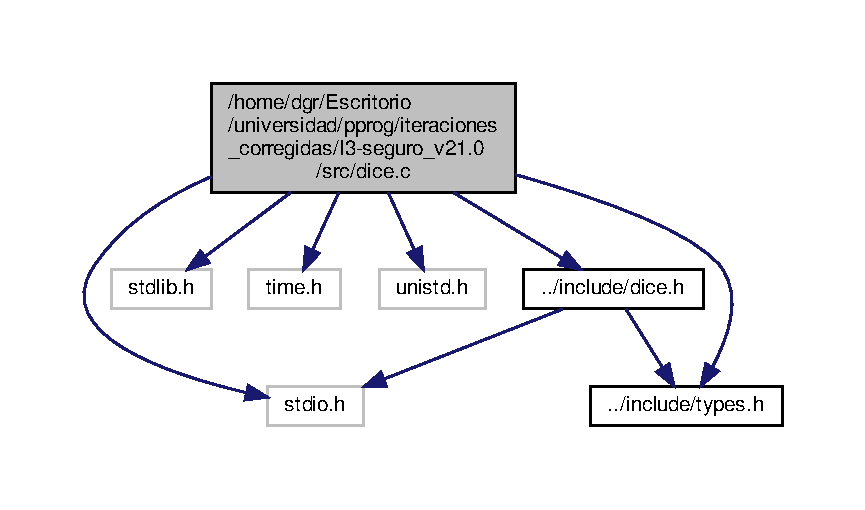
\includegraphics[width=350pt]{dice_8c__incl}
\end{center}
\end{figure}
\subsection*{Data Structures}
\begin{DoxyCompactItemize}
\item 
struct \hyperlink{struct__Dice}{\+\_\+\+Dice}
\begin{DoxyCompactList}\small\item\em The die structure. \end{DoxyCompactList}\end{DoxyCompactItemize}
\subsection*{Functions}
\begin{DoxyCompactItemize}
\item 
\hyperlink{dice_8h_a5910ae86cf402855269700abd23e3976}{Dice} $\ast$ \hyperlink{dice_8c_a6f5f18873cfd3e4da81b40e33c7cf637}{dice\+\_\+create} (\hyperlink{types_8h_a845e604fb28f7e3d97549da3448149d3}{Id} id, int max, int min)
\begin{DoxyCompactList}\small\item\em Create a dice. \end{DoxyCompactList}\item 
\hyperlink{types_8h_a32c27cc471df37f4fc818d65de0a56c4}{S\+T\+A\+T\+US} \hyperlink{dice_8c_a2c673e593f984c182dc6dde3f6dcfd59}{dice\+\_\+destroy} (\hyperlink{dice_8h_a5910ae86cf402855269700abd23e3976}{Dice} $\ast$dice)
\begin{DoxyCompactList}\small\item\em free a dice \end{DoxyCompactList}\item 
int \hyperlink{dice_8c_ab1ad7da98578cf2db3c70daffccfb944}{dice\+\_\+roll} (\hyperlink{dice_8h_a5910ae86cf402855269700abd23e3976}{Dice} $\ast$dice)
\begin{DoxyCompactList}\small\item\em roll a dice \end{DoxyCompactList}\item 
int \hyperlink{dice_8c_a2bfe1653c086f66149ba8fc3f3b52017}{dice\+\_\+get\+\_\+last} (\hyperlink{dice_8h_a5910ae86cf402855269700abd23e3976}{Dice} $\ast$dice)
\begin{DoxyCompactList}\small\item\em get the last roll value \end{DoxyCompactList}\item 
\hyperlink{types_8h_a32c27cc471df37f4fc818d65de0a56c4}{S\+T\+A\+T\+US} \hyperlink{dice_8c_adc188c44ee8d1058c574f08ac39b5c6b}{dice\+\_\+print} (\hyperlink{dice_8h_a5910ae86cf402855269700abd23e3976}{Dice} $\ast$dice)
\begin{DoxyCompactList}\small\item\em print a dice \end{DoxyCompactList}\end{DoxyCompactItemize}


\subsection{Detailed Description}
It implements the die interface. 

\begin{DoxyAuthor}{Author}
David Teófilo Garitagoitia Romero 
\end{DoxyAuthor}
\begin{DoxyVersion}{Version}
1.\+0 
\end{DoxyVersion}
\begin{DoxyDate}{Date}
20-\/02-\/2020 
\end{DoxyDate}
\begin{DoxyCopyright}{Copyright}
G\+NU Public License 
\end{DoxyCopyright}


\subsection{Function Documentation}
\mbox{\Hypertarget{dice_8c_a6f5f18873cfd3e4da81b40e33c7cf637}\label{dice_8c_a6f5f18873cfd3e4da81b40e33c7cf637}} 
\index{dice.\+c@{dice.\+c}!dice\+\_\+create@{dice\+\_\+create}}
\index{dice\+\_\+create@{dice\+\_\+create}!dice.\+c@{dice.\+c}}
\subsubsection{\texorpdfstring{dice\+\_\+create()}{dice\_create()}}
{\footnotesize\ttfamily \hyperlink{dice_8h_a5910ae86cf402855269700abd23e3976}{Dice}$\ast$ dice\+\_\+create (\begin{DoxyParamCaption}\item[{\hyperlink{types_8h_a845e604fb28f7e3d97549da3448149d3}{Id}}]{id,  }\item[{int}]{max,  }\item[{int}]{min }\end{DoxyParamCaption})}



Create a dice. 

dice\+\_\+create Create a dice with a specific Id, max and min

\begin{DoxyDate}{Date}
20-\/02-\/2019 
\end{DoxyDate}
\begin{DoxyAuthor}{Author}
David Teófilo Garitagoitia Romero
\end{DoxyAuthor}

\begin{DoxyParams}{Parameters}
{\em id} & the id of the new dice \\
\hline
{\em max} & the maximum of the dice \\
\hline
{\em min} & the minimum of the dice \\
\hline
\end{DoxyParams}
\begin{DoxyReturn}{Returns}
the new dice that has been created 
\end{DoxyReturn}
\mbox{\Hypertarget{dice_8c_a2c673e593f984c182dc6dde3f6dcfd59}\label{dice_8c_a2c673e593f984c182dc6dde3f6dcfd59}} 
\index{dice.\+c@{dice.\+c}!dice\+\_\+destroy@{dice\+\_\+destroy}}
\index{dice\+\_\+destroy@{dice\+\_\+destroy}!dice.\+c@{dice.\+c}}
\subsubsection{\texorpdfstring{dice\+\_\+destroy()}{dice\_destroy()}}
{\footnotesize\ttfamily \hyperlink{types_8h_a32c27cc471df37f4fc818d65de0a56c4}{S\+T\+A\+T\+US} dice\+\_\+destroy (\begin{DoxyParamCaption}\item[{\hyperlink{dice_8h_a5910ae86cf402855269700abd23e3976}{Dice} $\ast$}]{dice }\end{DoxyParamCaption})}



free a dice 

dice\+\_\+destroy free a especific dice

\begin{DoxyDate}{Date}
20-\/02-\/2019 
\end{DoxyDate}
\begin{DoxyAuthor}{Author}
David Teófilo Garitagoitia Romero
\end{DoxyAuthor}

\begin{DoxyParams}{Parameters}
{\em dice} & a dice that has been created before \\
\hline
\end{DoxyParams}
\begin{DoxyReturn}{Returns}
E\+R\+R\+OR if there is an error, otherwise return OK 
\end{DoxyReturn}
\mbox{\Hypertarget{dice_8c_a2bfe1653c086f66149ba8fc3f3b52017}\label{dice_8c_a2bfe1653c086f66149ba8fc3f3b52017}} 
\index{dice.\+c@{dice.\+c}!dice\+\_\+get\+\_\+last@{dice\+\_\+get\+\_\+last}}
\index{dice\+\_\+get\+\_\+last@{dice\+\_\+get\+\_\+last}!dice.\+c@{dice.\+c}}
\subsubsection{\texorpdfstring{dice\+\_\+get\+\_\+last()}{dice\_get\_last()}}
{\footnotesize\ttfamily int dice\+\_\+get\+\_\+last (\begin{DoxyParamCaption}\item[{\hyperlink{dice_8h_a5910ae86cf402855269700abd23e3976}{Dice} $\ast$}]{dice }\end{DoxyParamCaption})}



get the last roll value 

dice\+\_\+get\+\_\+last

\begin{DoxyDate}{Date}
20-\/02-\/2019 
\end{DoxyDate}
\begin{DoxyAuthor}{Author}
David Teófilo Garitagoitia Romero
\end{DoxyAuthor}

\begin{DoxyParams}{Parameters}
{\em dice} & a dice that has been created before \\
\hline
\end{DoxyParams}
\begin{DoxyReturn}{Returns}
-\/1 if there is an error, otherwise return the last roll value 
\end{DoxyReturn}
\mbox{\Hypertarget{dice_8c_adc188c44ee8d1058c574f08ac39b5c6b}\label{dice_8c_adc188c44ee8d1058c574f08ac39b5c6b}} 
\index{dice.\+c@{dice.\+c}!dice\+\_\+print@{dice\+\_\+print}}
\index{dice\+\_\+print@{dice\+\_\+print}!dice.\+c@{dice.\+c}}
\subsubsection{\texorpdfstring{dice\+\_\+print()}{dice\_print()}}
{\footnotesize\ttfamily \hyperlink{types_8h_a32c27cc471df37f4fc818d65de0a56c4}{S\+T\+A\+T\+US} dice\+\_\+print (\begin{DoxyParamCaption}\item[{\hyperlink{dice_8h_a5910ae86cf402855269700abd23e3976}{Dice} $\ast$}]{dice }\end{DoxyParamCaption})}



print a dice 

dice\+\_\+print print a especific dice

\begin{DoxyDate}{Date}
20-\/02-\/2019 
\end{DoxyDate}
\begin{DoxyAuthor}{Author}
David Teófilo Garitagoitia Romero
\end{DoxyAuthor}

\begin{DoxyParams}{Parameters}
{\em dice} & a dice which you want to print \\
\hline
\end{DoxyParams}
\begin{DoxyReturn}{Returns}
-\/1 if there is an error, otherwise return the number of the roll 
\end{DoxyReturn}
\mbox{\Hypertarget{dice_8c_ab1ad7da98578cf2db3c70daffccfb944}\label{dice_8c_ab1ad7da98578cf2db3c70daffccfb944}} 
\index{dice.\+c@{dice.\+c}!dice\+\_\+roll@{dice\+\_\+roll}}
\index{dice\+\_\+roll@{dice\+\_\+roll}!dice.\+c@{dice.\+c}}
\subsubsection{\texorpdfstring{dice\+\_\+roll()}{dice\_roll()}}
{\footnotesize\ttfamily int dice\+\_\+roll (\begin{DoxyParamCaption}\item[{\hyperlink{dice_8h_a5910ae86cf402855269700abd23e3976}{Dice} $\ast$}]{dice }\end{DoxyParamCaption})}



roll a dice 

dice\+\_\+roll roll a especific dice

\begin{DoxyDate}{Date}
20-\/02-\/2019 
\end{DoxyDate}
\begin{DoxyAuthor}{Author}
David Teófilo Garitagoitia Romero
\end{DoxyAuthor}

\begin{DoxyParams}{Parameters}
{\em dice} & a dice which you want to roll \\
\hline
\end{DoxyParams}
\begin{DoxyReturn}{Returns}
-\/1 if there is an error, otherwise return the number of the roll 
\end{DoxyReturn}

\hypertarget{dice__test_8c}{}\section{/home/dgr/\+Escritorio/universidad/pprog/iteraciones\+\_\+corregidas/\+I3-\/seguro\+\_\+v21.0/src/dice\+\_\+test.c File Reference}
\label{dice__test_8c}\index{/home/dgr/\+Escritorio/universidad/pprog/iteraciones\+\_\+corregidas/\+I3-\/seguro\+\_\+v21.\+0/src/dice\+\_\+test.\+c@{/home/dgr/\+Escritorio/universidad/pprog/iteraciones\+\_\+corregidas/\+I3-\/seguro\+\_\+v21.\+0/src/dice\+\_\+test.\+c}}


test to see if dice works correctly  


{\ttfamily \#include $<$stdio.\+h$>$}\newline
{\ttfamily \#include $<$stdlib.\+h$>$}\newline
{\ttfamily \#include \char`\"{}../include/test.\+h\char`\"{}}\newline
{\ttfamily \#include \char`\"{}../include/dice.\+h\char`\"{}}\newline
{\ttfamily \#include \char`\"{}../include/dice\+\_\+test.\+h\char`\"{}}\newline
Include dependency graph for dice\+\_\+test.\+c\+:
\nopagebreak
\begin{figure}[H]
\begin{center}
\leavevmode
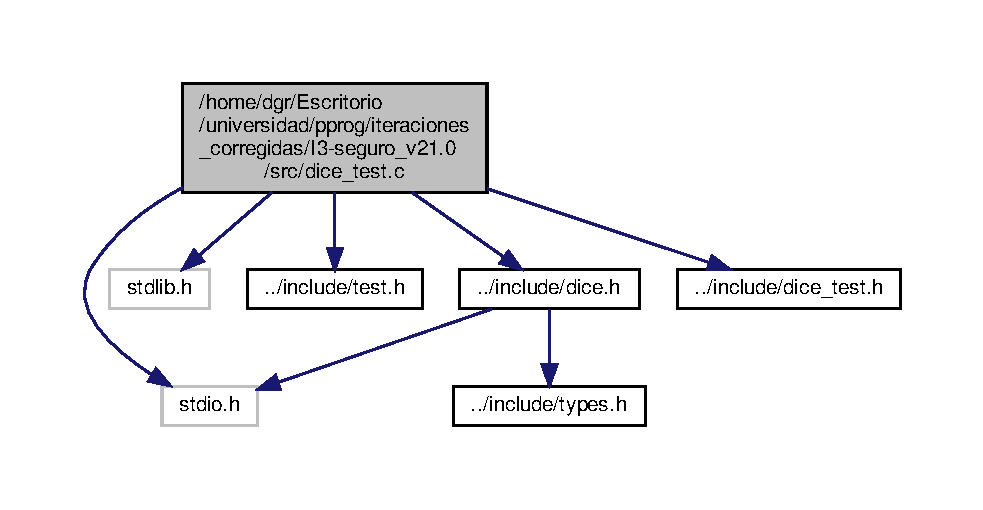
\includegraphics[width=350pt]{dice__test_8c__incl}
\end{center}
\end{figure}
\subsection*{Macros}
\begin{DoxyCompactItemize}
\item 
\#define \hyperlink{dice__test_8c_a2a77d2f2c5b698c69c19e1f8782bf709}{M\+A\+X\+\_\+\+T\+E\+S\+TS}~9
\begin{DoxyCompactList}\small\item\em maximum number of test \end{DoxyCompactList}\end{DoxyCompactItemize}
\subsection*{Functions}
\begin{DoxyCompactItemize}
\item 
int \hyperlink{dice__test_8c_a3c04138a5bfe5d72780bb7e82a18e627}{main} (int argc, char $\ast$$\ast$argv)
\begin{DoxyCompactList}\small\item\em the main function of dice\+\_\+test main \end{DoxyCompactList}\item 
void \hyperlink{dice__test_8c_afd8e7b7e3963ce0b48e40a7dcd4fb4b1}{test1\+\_\+dice\+\_\+create} ()
\item 
void \hyperlink{dice__test_8c_a3eacb7c8e4140ce2083d9705937f5106}{test2\+\_\+dice\+\_\+create} ()
\item 
void \hyperlink{dice__test_8c_a60f25d1250ef29f731d5e688fe989557}{test1\+\_\+dice\+\_\+roll} ()
\item 
void \hyperlink{dice__test_8c_a6c0509c7a5effe89212b9d786d9fc30c}{test2\+\_\+dice\+\_\+roll} ()
\item 
void \hyperlink{dice__test_8c_ab5b06d8e4cc2530d644b753d78a63314}{test3\+\_\+dice\+\_\+roll} ()
\item 
void \hyperlink{dice__test_8c_a3e678dfcb1adf09a85eb2e145088d053}{test1\+\_\+dice\+\_\+get\+\_\+last} ()
\item 
void \hyperlink{dice__test_8c_a5f15e643f69bfe582f6ffd548b92f846}{test2\+\_\+dice\+\_\+get\+\_\+last} ()
\item 
void \hyperlink{dice__test_8c_a80cc6894dcbee3feacca7da1b3cc82a3}{test3\+\_\+dice\+\_\+get\+\_\+last} ()
\item 
void \hyperlink{dice__test_8c_acfd69ccf21566f11ea0ccb8cc2f592ab}{test4\+\_\+dice\+\_\+get\+\_\+last} ()
\end{DoxyCompactItemize}


\subsection{Detailed Description}
test to see if dice works correctly 

\begin{DoxyAuthor}{Author}
Daniel Cerrato Sánchez 
\end{DoxyAuthor}
\begin{DoxyVersion}{Version}
2.\+0 
\end{DoxyVersion}
\begin{DoxyDate}{Date}
10-\/06-\/2020 
\end{DoxyDate}
\begin{DoxyCopyright}{Copyright}
G\+NU Public License 
\end{DoxyCopyright}


\subsection{Macro Definition Documentation}
\mbox{\Hypertarget{dice__test_8c_a2a77d2f2c5b698c69c19e1f8782bf709}\label{dice__test_8c_a2a77d2f2c5b698c69c19e1f8782bf709}} 
\index{dice\+\_\+test.\+c@{dice\+\_\+test.\+c}!M\+A\+X\+\_\+\+T\+E\+S\+TS@{M\+A\+X\+\_\+\+T\+E\+S\+TS}}
\index{M\+A\+X\+\_\+\+T\+E\+S\+TS@{M\+A\+X\+\_\+\+T\+E\+S\+TS}!dice\+\_\+test.\+c@{dice\+\_\+test.\+c}}
\subsubsection{\texorpdfstring{M\+A\+X\+\_\+\+T\+E\+S\+TS}{MAX\_TESTS}}
{\footnotesize\ttfamily \#define M\+A\+X\+\_\+\+T\+E\+S\+TS~9}



maximum number of test 

Details. 

\subsection{Function Documentation}
\mbox{\Hypertarget{dice__test_8c_a3c04138a5bfe5d72780bb7e82a18e627}\label{dice__test_8c_a3c04138a5bfe5d72780bb7e82a18e627}} 
\index{dice\+\_\+test.\+c@{dice\+\_\+test.\+c}!main@{main}}
\index{main@{main}!dice\+\_\+test.\+c@{dice\+\_\+test.\+c}}
\subsubsection{\texorpdfstring{main()}{main()}}
{\footnotesize\ttfamily int main (\begin{DoxyParamCaption}\item[{int}]{argc,  }\item[{char $\ast$$\ast$}]{argv }\end{DoxyParamCaption})}



the main function of dice\+\_\+test main 

\begin{DoxyDate}{Date}
10-\/06-\/2020 
\end{DoxyDate}
\begin{DoxyAuthor}{Author}
Daniel Cerrato Sánchez 
\end{DoxyAuthor}
\begin{DoxyReturn}{Returns}

\end{DoxyReturn}
\mbox{\Hypertarget{dice__test_8c_afd8e7b7e3963ce0b48e40a7dcd4fb4b1}\label{dice__test_8c_afd8e7b7e3963ce0b48e40a7dcd4fb4b1}} 
\index{dice\+\_\+test.\+c@{dice\+\_\+test.\+c}!test1\+\_\+dice\+\_\+create@{test1\+\_\+dice\+\_\+create}}
\index{test1\+\_\+dice\+\_\+create@{test1\+\_\+dice\+\_\+create}!dice\+\_\+test.\+c@{dice\+\_\+test.\+c}}
\subsubsection{\texorpdfstring{test1\+\_\+dice\+\_\+create()}{test1\_dice\_create()}}
{\footnotesize\ttfamily void test1\+\_\+dice\+\_\+create (\begin{DoxyParamCaption}{ }\end{DoxyParamCaption})}

\begin{DoxyRefDesc}{Test}
\item[\hyperlink{test__test000048}{Test}]Test the dice creation function \end{DoxyRefDesc}
\begin{DoxyPrecond}{Precondition}
An id, a maximum value and a minimum value in integer value as parameters, the maximum is greater than the minimum 
\end{DoxyPrecond}
\begin{DoxyPostcond}{Postcondition}
A non-\/null pointer to the created die 
\end{DoxyPostcond}
\mbox{\Hypertarget{dice__test_8c_a3e678dfcb1adf09a85eb2e145088d053}\label{dice__test_8c_a3e678dfcb1adf09a85eb2e145088d053}} 
\index{dice\+\_\+test.\+c@{dice\+\_\+test.\+c}!test1\+\_\+dice\+\_\+get\+\_\+last@{test1\+\_\+dice\+\_\+get\+\_\+last}}
\index{test1\+\_\+dice\+\_\+get\+\_\+last@{test1\+\_\+dice\+\_\+get\+\_\+last}!dice\+\_\+test.\+c@{dice\+\_\+test.\+c}}
\subsubsection{\texorpdfstring{test1\+\_\+dice\+\_\+get\+\_\+last()}{test1\_dice\_get\_last()}}
{\footnotesize\ttfamily void test1\+\_\+dice\+\_\+get\+\_\+last (\begin{DoxyParamCaption}{ }\end{DoxyParamCaption})}

\begin{DoxyRefDesc}{Test}
\item[\hyperlink{test__test000053}{Test}]Test the function to get the last value taken with the given \end{DoxyRefDesc}
\begin{DoxyPrecond}{Precondition}
The die is a non-\/\+N\+U\+LL pointer with the correct fields, after having thrown 
\end{DoxyPrecond}
\begin{DoxyPostcond}{Postcondition}
The output must be greater than or equal to the minimum value entered 
\end{DoxyPostcond}
\mbox{\Hypertarget{dice__test_8c_a60f25d1250ef29f731d5e688fe989557}\label{dice__test_8c_a60f25d1250ef29f731d5e688fe989557}} 
\index{dice\+\_\+test.\+c@{dice\+\_\+test.\+c}!test1\+\_\+dice\+\_\+roll@{test1\+\_\+dice\+\_\+roll}}
\index{test1\+\_\+dice\+\_\+roll@{test1\+\_\+dice\+\_\+roll}!dice\+\_\+test.\+c@{dice\+\_\+test.\+c}}
\subsubsection{\texorpdfstring{test1\+\_\+dice\+\_\+roll()}{test1\_dice\_roll()}}
{\footnotesize\ttfamily void test1\+\_\+dice\+\_\+roll (\begin{DoxyParamCaption}{ }\end{DoxyParamCaption})}

\begin{DoxyRefDesc}{Test}
\item[\hyperlink{test__test000050}{Test}]Test the function to get a value from the dice \end{DoxyRefDesc}
\begin{DoxyPrecond}{Precondition}
The die is a non-\/\+N\+U\+LL pointer with the correct fields 
\end{DoxyPrecond}
\begin{DoxyPostcond}{Postcondition}
The output must be greater than or equal to the minimum value entered 
\end{DoxyPostcond}
\mbox{\Hypertarget{dice__test_8c_a3eacb7c8e4140ce2083d9705937f5106}\label{dice__test_8c_a3eacb7c8e4140ce2083d9705937f5106}} 
\index{dice\+\_\+test.\+c@{dice\+\_\+test.\+c}!test2\+\_\+dice\+\_\+create@{test2\+\_\+dice\+\_\+create}}
\index{test2\+\_\+dice\+\_\+create@{test2\+\_\+dice\+\_\+create}!dice\+\_\+test.\+c@{dice\+\_\+test.\+c}}
\subsubsection{\texorpdfstring{test2\+\_\+dice\+\_\+create()}{test2\_dice\_create()}}
{\footnotesize\ttfamily void test2\+\_\+dice\+\_\+create (\begin{DoxyParamCaption}{ }\end{DoxyParamCaption})}

\begin{DoxyRefDesc}{Test}
\item[\hyperlink{test__test000049}{Test}]Test the dice creation function \end{DoxyRefDesc}
\begin{DoxyPrecond}{Precondition}
An id, a maximum value and a minimum value in integer value as parameters, the minimum is greater than the maximum 
\end{DoxyPrecond}
\begin{DoxyPostcond}{Postcondition}
A null pointer to the created die 
\end{DoxyPostcond}
\mbox{\Hypertarget{dice__test_8c_a5f15e643f69bfe582f6ffd548b92f846}\label{dice__test_8c_a5f15e643f69bfe582f6ffd548b92f846}} 
\index{dice\+\_\+test.\+c@{dice\+\_\+test.\+c}!test2\+\_\+dice\+\_\+get\+\_\+last@{test2\+\_\+dice\+\_\+get\+\_\+last}}
\index{test2\+\_\+dice\+\_\+get\+\_\+last@{test2\+\_\+dice\+\_\+get\+\_\+last}!dice\+\_\+test.\+c@{dice\+\_\+test.\+c}}
\subsubsection{\texorpdfstring{test2\+\_\+dice\+\_\+get\+\_\+last()}{test2\_dice\_get\_last()}}
{\footnotesize\ttfamily void test2\+\_\+dice\+\_\+get\+\_\+last (\begin{DoxyParamCaption}{ }\end{DoxyParamCaption})}

\begin{DoxyRefDesc}{Test}
\item[\hyperlink{test__test000054}{Test}]Test the function to get the last value taken with the given \end{DoxyRefDesc}
\begin{DoxyPrecond}{Precondition}
The die is a non-\/\+N\+U\+LL pointer with the correct fields, after having thrown 
\end{DoxyPrecond}
\begin{DoxyPostcond}{Postcondition}
The output must be less than or equal to the maximum value entered 
\end{DoxyPostcond}
\mbox{\Hypertarget{dice__test_8c_a6c0509c7a5effe89212b9d786d9fc30c}\label{dice__test_8c_a6c0509c7a5effe89212b9d786d9fc30c}} 
\index{dice\+\_\+test.\+c@{dice\+\_\+test.\+c}!test2\+\_\+dice\+\_\+roll@{test2\+\_\+dice\+\_\+roll}}
\index{test2\+\_\+dice\+\_\+roll@{test2\+\_\+dice\+\_\+roll}!dice\+\_\+test.\+c@{dice\+\_\+test.\+c}}
\subsubsection{\texorpdfstring{test2\+\_\+dice\+\_\+roll()}{test2\_dice\_roll()}}
{\footnotesize\ttfamily void test2\+\_\+dice\+\_\+roll (\begin{DoxyParamCaption}{ }\end{DoxyParamCaption})}

\begin{DoxyRefDesc}{Test}
\item[\hyperlink{test__test000051}{Test}]Test the function to get a value from the dice \end{DoxyRefDesc}
\begin{DoxyPrecond}{Precondition}
The die is a non-\/\+N\+U\+LL pointer with the correct fields 
\end{DoxyPrecond}
\begin{DoxyPostcond}{Postcondition}
The output must be less than or equal to the maximum value entered 
\end{DoxyPostcond}
\mbox{\Hypertarget{dice__test_8c_a80cc6894dcbee3feacca7da1b3cc82a3}\label{dice__test_8c_a80cc6894dcbee3feacca7da1b3cc82a3}} 
\index{dice\+\_\+test.\+c@{dice\+\_\+test.\+c}!test3\+\_\+dice\+\_\+get\+\_\+last@{test3\+\_\+dice\+\_\+get\+\_\+last}}
\index{test3\+\_\+dice\+\_\+get\+\_\+last@{test3\+\_\+dice\+\_\+get\+\_\+last}!dice\+\_\+test.\+c@{dice\+\_\+test.\+c}}
\subsubsection{\texorpdfstring{test3\+\_\+dice\+\_\+get\+\_\+last()}{test3\_dice\_get\_last()}}
{\footnotesize\ttfamily void test3\+\_\+dice\+\_\+get\+\_\+last (\begin{DoxyParamCaption}{ }\end{DoxyParamCaption})}

\begin{DoxyRefDesc}{Test}
\item[\hyperlink{test__test000055}{Test}]Test the function to get the last value taken with the given \end{DoxyRefDesc}
\begin{DoxyPrecond}{Precondition}
The die is a non-\/\+N\+U\+LL pointer with the correct fields, without having thrown 
\end{DoxyPrecond}
\begin{DoxyPostcond}{Postcondition}
The output must be 0 
\end{DoxyPostcond}
\mbox{\Hypertarget{dice__test_8c_ab5b06d8e4cc2530d644b753d78a63314}\label{dice__test_8c_ab5b06d8e4cc2530d644b753d78a63314}} 
\index{dice\+\_\+test.\+c@{dice\+\_\+test.\+c}!test3\+\_\+dice\+\_\+roll@{test3\+\_\+dice\+\_\+roll}}
\index{test3\+\_\+dice\+\_\+roll@{test3\+\_\+dice\+\_\+roll}!dice\+\_\+test.\+c@{dice\+\_\+test.\+c}}
\subsubsection{\texorpdfstring{test3\+\_\+dice\+\_\+roll()}{test3\_dice\_roll()}}
{\footnotesize\ttfamily void test3\+\_\+dice\+\_\+roll (\begin{DoxyParamCaption}{ }\end{DoxyParamCaption})}

\begin{DoxyRefDesc}{Test}
\item[\hyperlink{test__test000052}{Test}]Test the function to get a value from the dice \end{DoxyRefDesc}
\begin{DoxyPrecond}{Precondition}
The die is a pointer to N\+U\+LL 
\end{DoxyPrecond}
\begin{DoxyPostcond}{Postcondition}
The output must be -\/1 
\end{DoxyPostcond}
\mbox{\Hypertarget{dice__test_8c_acfd69ccf21566f11ea0ccb8cc2f592ab}\label{dice__test_8c_acfd69ccf21566f11ea0ccb8cc2f592ab}} 
\index{dice\+\_\+test.\+c@{dice\+\_\+test.\+c}!test4\+\_\+dice\+\_\+get\+\_\+last@{test4\+\_\+dice\+\_\+get\+\_\+last}}
\index{test4\+\_\+dice\+\_\+get\+\_\+last@{test4\+\_\+dice\+\_\+get\+\_\+last}!dice\+\_\+test.\+c@{dice\+\_\+test.\+c}}
\subsubsection{\texorpdfstring{test4\+\_\+dice\+\_\+get\+\_\+last()}{test4\_dice\_get\_last()}}
{\footnotesize\ttfamily void test4\+\_\+dice\+\_\+get\+\_\+last (\begin{DoxyParamCaption}{ }\end{DoxyParamCaption})}

\begin{DoxyRefDesc}{Test}
\item[\hyperlink{test__test000056}{Test}]Test the function to get the last value taken with the given \end{DoxyRefDesc}
\begin{DoxyPrecond}{Precondition}
The die is a pointer to N\+U\+LL 
\end{DoxyPrecond}
\begin{DoxyPostcond}{Postcondition}
The output must be -\/1 
\end{DoxyPostcond}

\hypertarget{game_8c}{}\section{/home/dgr/\+Escritorio/universidad/pprog/iteraciones\+\_\+corregidas/\+I3-\/seguro\+\_\+v21.0/src/game.c File Reference}
\label{game_8c}\index{/home/dgr/\+Escritorio/universidad/pprog/iteraciones\+\_\+corregidas/\+I3-\/seguro\+\_\+v21.\+0/src/game.\+c@{/home/dgr/\+Escritorio/universidad/pprog/iteraciones\+\_\+corregidas/\+I3-\/seguro\+\_\+v21.\+0/src/game.\+c}}


It implements the game interface and all the associated callbacks for each command.  


{\ttfamily \#include $<$stdio.\+h$>$}\newline
{\ttfamily \#include $<$stdlib.\+h$>$}\newline
{\ttfamily \#include $<$string.\+h$>$}\newline
{\ttfamily \#include \char`\"{}../include/game.\+h\char`\"{}}\newline
{\ttfamily \#include \char`\"{}../include/space.\+h\char`\"{}}\newline
{\ttfamily \#include \char`\"{}../include/game\+\_\+reader.\+h\char`\"{}}\newline
{\ttfamily \#include \char`\"{}../include/player.\+h\char`\"{}}\newline
{\ttfamily \#include \char`\"{}../include/object.\+h\char`\"{}}\newline
{\ttfamily \#include \char`\"{}../include/inventory.\+h\char`\"{}}\newline
{\ttfamily \#include \char`\"{}../include/link.\+h\char`\"{}}\newline
Include dependency graph for game.\+c\+:
\nopagebreak
\begin{figure}[H]
\begin{center}
\leavevmode
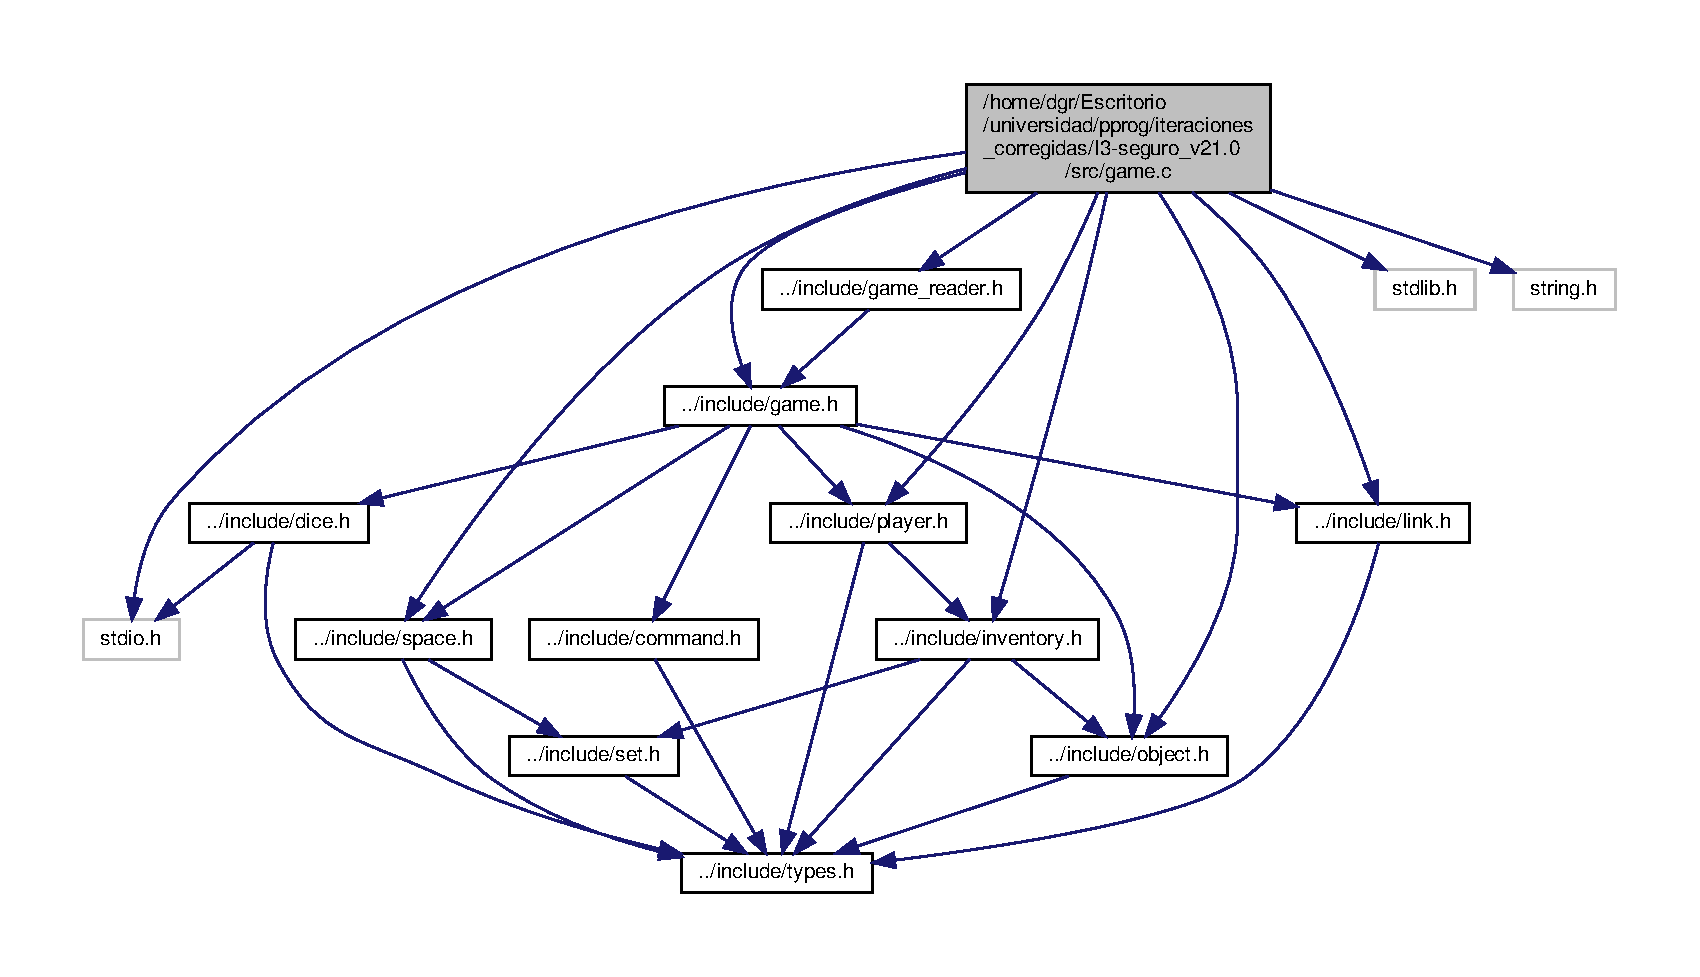
\includegraphics[width=350pt]{game_8c__incl}
\end{center}
\end{figure}
\subsection*{Data Structures}
\begin{DoxyCompactItemize}
\item 
struct \hyperlink{struct__Game}{\+\_\+\+Game}
\begin{DoxyCompactList}\small\item\em The game structure. \end{DoxyCompactList}\end{DoxyCompactItemize}
\subsection*{Macros}
\begin{DoxyCompactItemize}
\item 
\#define \hyperlink{game_8c_a8366e5ad74afbbea0cd0a414770c304a}{N\+\_\+\+C\+A\+L\+L\+B\+A\+CK}~11
\begin{DoxyCompactList}\small\item\em A macro that stores the number of callbacks. \end{DoxyCompactList}\item 
\#define \hyperlink{game_8c_ae9c24f3b396f6bdaacd0e52f68b9a314}{gp}~16
\begin{DoxyCompactList}\small\item\em A macro that stores the number of chars used on graphic description. \end{DoxyCompactList}\end{DoxyCompactItemize}
\subsection*{Typedefs}
\begin{DoxyCompactItemize}
\item 
typedef void($\ast$ \hyperlink{game_8c_ac54a175bdefaeb274c3515fc6f43dbe5}{callback\+\_\+fn}) (\hyperlink{game_8h_a57156d39c530aec3fba3a9dad8c2dc6a}{Game} $\ast$game)
\end{DoxyCompactItemize}
\subsection*{Functions}
\begin{DoxyCompactItemize}
\item 
\hyperlink{types_8h_a845e604fb28f7e3d97549da3448149d3}{Id} \hyperlink{game_8c_acab53bacb2b0920f8f1e34e835817369}{game\+\_\+get\+\_\+object\+\_\+id\+\_\+at\+\_\+name} (\hyperlink{game_8h_a57156d39c530aec3fba3a9dad8c2dc6a}{Game} $\ast$game, char $\ast$name)
\begin{DoxyCompactList}\small\item\em function to get object id at their name game\+\_\+get\+\_\+object\+\_\+id\+\_\+at\+\_\+name \end{DoxyCompactList}\item 
\hyperlink{object_8h_a7f8bbcda919b65ce67f92fba08e0212f}{Object} $\ast$ \hyperlink{game_8c_a7df5a5ffd7da77b78c268fca096eee2b}{game\+\_\+get\+\_\+object\+\_\+at\+\_\+id} (\hyperlink{game_8h_a57156d39c530aec3fba3a9dad8c2dc6a}{Game} $\ast$game, \hyperlink{types_8h_a845e604fb28f7e3d97549da3448149d3}{Id} id)
\begin{DoxyCompactList}\small\item\em function to get object at their name game\+\_\+get\+\_\+object\+\_\+at\+\_\+id \end{DoxyCompactList}\item 
void \hyperlink{game_8c_ac8ed327ed13f97dcb778d0293f14d8bb}{game\+\_\+callback\+\_\+unknown} (\hyperlink{game_8h_a57156d39c530aec3fba3a9dad8c2dc6a}{Game} $\ast$game)
\begin{DoxyCompactList}\small\item\em the callback to unknow command game\+\_\+callback\+\_\+unknown \end{DoxyCompactList}\item 
void \hyperlink{game_8c_acc98d79a418d2093fc3224b5c02e5418}{game\+\_\+callback\+\_\+exit} (\hyperlink{game_8h_a57156d39c530aec3fba3a9dad8c2dc6a}{Game} $\ast$game)
\begin{DoxyCompactList}\small\item\em the callback to exit command game\+\_\+callback\+\_\+exit \end{DoxyCompactList}\item 
void \hyperlink{game_8c_aabbe11eeeb10b57d1262f28b51cad8f9}{game\+\_\+callback\+\_\+take} (\hyperlink{game_8h_a57156d39c530aec3fba3a9dad8c2dc6a}{Game} $\ast$game)
\begin{DoxyCompactList}\small\item\em the callback to take command game\+\_\+callback\+\_\+take \end{DoxyCompactList}\item 
void \hyperlink{game_8c_a424d0c659a926b0588a4287ea82552b6}{game\+\_\+callback\+\_\+drop} (\hyperlink{game_8h_a57156d39c530aec3fba3a9dad8c2dc6a}{Game} $\ast$game)
\begin{DoxyCompactList}\small\item\em the callback to drop command game\+\_\+callback\+\_\+drop \end{DoxyCompactList}\item 
void \hyperlink{game_8c_a4929c380e741fce955cb09ad3058e6d7}{game\+\_\+callback\+\_\+roll} (\hyperlink{game_8h_a57156d39c530aec3fba3a9dad8c2dc6a}{Game} $\ast$game)
\begin{DoxyCompactList}\small\item\em the callback to roll command game\+\_\+callback\+\_\+roll \end{DoxyCompactList}\item 
void \hyperlink{game_8c_a7525cbe807f8d1c3b698afcb75903903}{game\+\_\+callback\+\_\+move} (\hyperlink{game_8h_a57156d39c530aec3fba3a9dad8c2dc6a}{Game} $\ast$game)
\begin{DoxyCompactList}\small\item\em the callback to move command game\+\_\+callback\+\_\+roll \end{DoxyCompactList}\item 
void \hyperlink{game_8c_aa4e4f958e69b85fc4ddbb1c44a0bfce7}{game\+\_\+callback\+\_\+inspect} (\hyperlink{game_8h_a57156d39c530aec3fba3a9dad8c2dc6a}{Game} $\ast$game)
\begin{DoxyCompactList}\small\item\em the callback to inspect command game\+\_\+callback\+\_\+inspect \end{DoxyCompactList}\item 
void \hyperlink{game_8c_a19e44ed4634989f22a55f8b5bbe84cb9}{game\+\_\+callback\+\_\+next} (\hyperlink{game_8h_a57156d39c530aec3fba3a9dad8c2dc6a}{Game} $\ast$game)
\begin{DoxyCompactList}\small\item\em the callback to next command game\+\_\+callback\+\_\+next \end{DoxyCompactList}\item 
void \hyperlink{game_8c_a8fe7c0d05fb65537bc4d9304bafe916e}{game\+\_\+callback\+\_\+back} (\hyperlink{game_8h_a57156d39c530aec3fba3a9dad8c2dc6a}{Game} $\ast$game)
\begin{DoxyCompactList}\small\item\em the callback to back command game\+\_\+callback\+\_\+back \end{DoxyCompactList}\item 
void \hyperlink{game_8c_a39f7f8f01c726f24880be16b0d6d5d9f}{game\+\_\+callback\+\_\+left} (\hyperlink{game_8h_a57156d39c530aec3fba3a9dad8c2dc6a}{Game} $\ast$game)
\begin{DoxyCompactList}\small\item\em the callback to left command game\+\_\+callback\+\_\+left \end{DoxyCompactList}\item 
void \hyperlink{game_8c_a28b96a72f634d9535af0618950980728}{game\+\_\+callback\+\_\+right} (\hyperlink{game_8h_a57156d39c530aec3fba3a9dad8c2dc6a}{Game} $\ast$game)
\begin{DoxyCompactList}\small\item\em the callback to right command game\+\_\+callback\+\_\+right \end{DoxyCompactList}\item 
\hyperlink{game_8h_a57156d39c530aec3fba3a9dad8c2dc6a}{Game} $\ast$ \hyperlink{game_8c_a1cdbe3f06b9bf49eb5e334a22ad3b2b9}{game\+\_\+create} ()
\begin{DoxyCompactList}\small\item\em Create the game, initialite the variables of the game. \end{DoxyCompactList}\item 
\hyperlink{game_8h_a57156d39c530aec3fba3a9dad8c2dc6a}{Game} $\ast$ \hyperlink{game_8c_a0e225eaf98598147fdfba6fed2ea8f02}{game\+\_\+create\+\_\+from\+\_\+file} (char $\ast$filename)
\begin{DoxyCompactList}\small\item\em Create the game from a file. \end{DoxyCompactList}\item 
\hyperlink{link_8h_ae3b299941e67be6971bfd64a25505eff}{Link} $\ast$ \hyperlink{game_8c_a34824b782ef05dcca98e83546b321ebf}{game\+\_\+get\+\_\+link\+\_\+at\+\_\+id} (\hyperlink{game_8h_a57156d39c530aec3fba3a9dad8c2dc6a}{Game} $\ast$game, \hyperlink{types_8h_a845e604fb28f7e3d97549da3448149d3}{Id} id)
\begin{DoxyCompactList}\small\item\em return a link pointer from their id \end{DoxyCompactList}\item 
\hyperlink{types_8h_a845e604fb28f7e3d97549da3448149d3}{Id} \hyperlink{game_8c_ab08e136689431b2c932cfcac2131c51a}{game\+\_\+get\+\_\+south} (\hyperlink{game_8h_a57156d39c530aec3fba3a9dad8c2dc6a}{Game} $\ast$game, \hyperlink{space_8h_a67533ffc2b70463baecc38fb0629bbfc}{Space} $\ast$space)
\begin{DoxyCompactList}\small\item\em returns the id of the souther link of the space \end{DoxyCompactList}\item 
\hyperlink{types_8h_a845e604fb28f7e3d97549da3448149d3}{Id} \hyperlink{game_8c_a19a5cd5f4230efccff68d10af5af40e8}{game\+\_\+get\+\_\+north} (\hyperlink{game_8h_a57156d39c530aec3fba3a9dad8c2dc6a}{Game} $\ast$game, \hyperlink{space_8h_a67533ffc2b70463baecc38fb0629bbfc}{Space} $\ast$space)
\begin{DoxyCompactList}\small\item\em returns the id of the north link of the space \end{DoxyCompactList}\item 
\hyperlink{types_8h_a845e604fb28f7e3d97549da3448149d3}{Id} \hyperlink{game_8c_a23b7636aa7306962aaf1358697cabd76}{game\+\_\+get\+\_\+east} (\hyperlink{game_8h_a57156d39c530aec3fba3a9dad8c2dc6a}{Game} $\ast$game, \hyperlink{space_8h_a67533ffc2b70463baecc38fb0629bbfc}{Space} $\ast$space)
\begin{DoxyCompactList}\small\item\em returns the id of the east link of the space \end{DoxyCompactList}\item 
\hyperlink{types_8h_a845e604fb28f7e3d97549da3448149d3}{Id} \hyperlink{game_8c_ad86395a448cc3e6100cdcef36427d840}{game\+\_\+get\+\_\+west} (\hyperlink{game_8h_a57156d39c530aec3fba3a9dad8c2dc6a}{Game} $\ast$game, \hyperlink{space_8h_a67533ffc2b70463baecc38fb0629bbfc}{Space} $\ast$space)
\begin{DoxyCompactList}\small\item\em returns the id of the west link of the space \end{DoxyCompactList}\item 
\hyperlink{types_8h_a32c27cc471df37f4fc818d65de0a56c4}{S\+T\+A\+T\+US} \hyperlink{game_8c_a9597a8e456aa74db536e87d56f56c3b4}{game\+\_\+add\+\_\+object} (\hyperlink{game_8h_a57156d39c530aec3fba3a9dad8c2dc6a}{Game} $\ast$game, \hyperlink{object_8h_a7f8bbcda919b65ce67f92fba08e0212f}{Object} $\ast$object)
\begin{DoxyCompactList}\small\item\em add a new object to the game \end{DoxyCompactList}\item 
\hyperlink{types_8h_a845e604fb28f7e3d97549da3448149d3}{Id} \hyperlink{game_8c_a83b86a040470f67786d912f45efc9eb8}{game\+\_\+get\+\_\+object\+\_\+location} (\hyperlink{game_8h_a57156d39c530aec3fba3a9dad8c2dc6a}{Game} $\ast$game, \hyperlink{types_8h_a845e604fb28f7e3d97549da3448149d3}{Id} object)
\begin{DoxyCompactList}\small\item\em get the location of an object \end{DoxyCompactList}\item 
\hyperlink{types_8h_a32c27cc471df37f4fc818d65de0a56c4}{S\+T\+A\+T\+US} \hyperlink{game_8c_a0736924a1235c0e6fe9b6d91c2a12af8}{game\+\_\+destroy} (\hyperlink{game_8h_a57156d39c530aec3fba3a9dad8c2dc6a}{Game} $\ast$game)
\begin{DoxyCompactList}\small\item\em free the game \end{DoxyCompactList}\item 
\hyperlink{types_8h_a32c27cc471df37f4fc818d65de0a56c4}{S\+T\+A\+T\+US} \hyperlink{game_8c_a8711cf50c2cef44e064da433807e252a}{game\+\_\+update} (\hyperlink{game_8h_a57156d39c530aec3fba3a9dad8c2dc6a}{Game} $\ast$game, \hyperlink{command_8h_a0473597db8c45c0289b6b8e2f8abbe32}{T\+\_\+\+Command} command, char $\ast$argument)
\begin{DoxyCompactList}\small\item\em update the game \end{DoxyCompactList}\item 
\hyperlink{types_8h_a32c27cc471df37f4fc818d65de0a56c4}{S\+T\+A\+T\+US} \hyperlink{game_8c_ae5ad86de0a92d9eccb234948458da7f1}{game\+\_\+add\+\_\+space} (\hyperlink{game_8h_a57156d39c530aec3fba3a9dad8c2dc6a}{Game} $\ast$game, \hyperlink{space_8h_a67533ffc2b70463baecc38fb0629bbfc}{Space} $\ast$space)
\begin{DoxyCompactList}\small\item\em add a space in the game \end{DoxyCompactList}\item 
\hyperlink{types_8h_a32c27cc471df37f4fc818d65de0a56c4}{S\+T\+A\+T\+US} \hyperlink{game_8c_a4691bee17d5784ad6eb257dfbb252c27}{game\+\_\+add\+\_\+link} (\hyperlink{game_8h_a57156d39c530aec3fba3a9dad8c2dc6a}{Game} $\ast$game, \hyperlink{link_8h_ae3b299941e67be6971bfd64a25505eff}{Link} $\ast$link)
\begin{DoxyCompactList}\small\item\em add a link to the game \end{DoxyCompactList}\item 
\hyperlink{types_8h_a32c27cc471df37f4fc818d65de0a56c4}{S\+T\+A\+T\+US} \hyperlink{game_8c_ade0d25f267771b1f9b27fcc0383e93b8}{game\+\_\+set\+\_\+player} (\hyperlink{game_8h_a57156d39c530aec3fba3a9dad8c2dc6a}{Game} $\ast$game, \hyperlink{player_8h_af30e2030635a69690f85e48bc6ef202f}{Player} $\ast$player)
\begin{DoxyCompactList}\small\item\em set the player of the game \end{DoxyCompactList}\item 
\hyperlink{types_8h_a845e604fb28f7e3d97549da3448149d3}{Id} \hyperlink{game_8c_ad2dfd865e2bd2c545a15d33f4d1cf3ae}{game\+\_\+get\+\_\+space\+\_\+id\+\_\+at} (\hyperlink{game_8h_a57156d39c530aec3fba3a9dad8c2dc6a}{Game} $\ast$game, int position)
\begin{DoxyCompactList}\small\item\em return the id of an space form their position \end{DoxyCompactList}\item 
\hyperlink{space_8h_a67533ffc2b70463baecc38fb0629bbfc}{Space} $\ast$ \hyperlink{game_8c_a69d94da9d27b542d3ebdeb8b60f1f2dc}{game\+\_\+get\+\_\+space} (\hyperlink{game_8h_a57156d39c530aec3fba3a9dad8c2dc6a}{Game} $\ast$game, \hyperlink{types_8h_a845e604fb28f7e3d97549da3448149d3}{Id} id)
\begin{DoxyCompactList}\small\item\em get the space \end{DoxyCompactList}\item 
\hyperlink{command_8h_a0473597db8c45c0289b6b8e2f8abbe32}{T\+\_\+\+Command} \hyperlink{game_8c_ac6c33f046d4854d4357ca95428a41281}{game\+\_\+get\+\_\+last\+\_\+principal\+\_\+command} (\hyperlink{game_8h_a57156d39c530aec3fba3a9dad8c2dc6a}{Game} $\ast$game)
\begin{DoxyCompactList}\small\item\em get the last command of the game \end{DoxyCompactList}\item 
\hyperlink{command_8h_a7d2935971c252377cb0fc1c8545dc2bc}{Command} $\ast$ \hyperlink{game_8c_a0622ea04a0e30e49f51ed4c83257bee5}{game\+\_\+get\+\_\+last\+\_\+command} (\hyperlink{game_8h_a57156d39c530aec3fba3a9dad8c2dc6a}{Game} $\ast$game)
\begin{DoxyCompactList}\small\item\em get the comand insert by the user \end{DoxyCompactList}\item 
char $\ast$ \hyperlink{game_8c_a89c667c3db1a1afe426c264a742d373c}{game\+\_\+get\+\_\+last\+\_\+argument} (\hyperlink{game_8h_a57156d39c530aec3fba3a9dad8c2dc6a}{Game} $\ast$game)
\begin{DoxyCompactList}\small\item\em get the argument insert by the user \end{DoxyCompactList}\item 
const char $\ast$ \hyperlink{game_8c_a2ecf68dd442c912c2b0da3c3dd9fef9e}{game\+\_\+get\+\_\+object\+\_\+name\+\_\+at\+\_\+id} (\hyperlink{game_8h_a57156d39c530aec3fba3a9dad8c2dc6a}{Game} $\ast$game, \hyperlink{types_8h_a845e604fb28f7e3d97549da3448149d3}{Id} id)
\begin{DoxyCompactList}\small\item\em return the name of an object from his id \end{DoxyCompactList}\item 
void \hyperlink{game_8c_a81ff7aff49ff47a7a16a88df4ae06956}{game\+\_\+get\+\_\+objects\+\_\+name\+\_\+at\+\_\+space} (\hyperlink{space_8h_a67533ffc2b70463baecc38fb0629bbfc}{Space} $\ast$space, \hyperlink{game_8h_a57156d39c530aec3fba3a9dad8c2dc6a}{Game} $\ast$game, char $\ast$names)
\begin{DoxyCompactList}\small\item\em save a string with the name of all objects of an space in the names argument \end{DoxyCompactList}\item 
void \hyperlink{game_8c_ab13626a54ff51e2300a82f5c6ebd6ec7}{game\+\_\+get\+\_\+player\+\_\+objects} (\hyperlink{game_8h_a57156d39c530aec3fba3a9dad8c2dc6a}{Game} $\ast$game, char $\ast$names)
\begin{DoxyCompactList}\small\item\em get the player objects of the game \end{DoxyCompactList}\item 
void \hyperlink{game_8c_ab6154c70ef6dd43b0dc7089d6f363974}{game\+\_\+get\+\_\+objects\+\_\+location} (\hyperlink{game_8h_a57156d39c530aec3fba3a9dad8c2dc6a}{Game} $\ast$game, char $\ast$names)
\begin{DoxyCompactList}\small\item\em save a string with the name of all objects of the game and their locations in the names argument \end{DoxyCompactList}\item 
void \hyperlink{game_8c_a33a5ed8937423f8c012df3cedad4fa4c}{game\+\_\+print\+\_\+data} (\hyperlink{game_8h_a57156d39c530aec3fba3a9dad8c2dc6a}{Game} $\ast$game)
\begin{DoxyCompactList}\small\item\em print the game data \end{DoxyCompactList}\item 
\hyperlink{player_8h_af30e2030635a69690f85e48bc6ef202f}{Player} $\ast$ \hyperlink{game_8c_af46efd507d797aec6da90d08aa592e32}{game\+\_\+get\+\_\+player} (\hyperlink{game_8h_a57156d39c530aec3fba3a9dad8c2dc6a}{Game} $\ast$game)
\begin{DoxyCompactList}\small\item\em get the player of the game \end{DoxyCompactList}\item 
\hyperlink{dice_8h_a5910ae86cf402855269700abd23e3976}{Dice} $\ast$ \hyperlink{game_8c_ab32e231181826f82db6c6d161d2eb647}{game\+\_\+get\+\_\+dice} (\hyperlink{game_8h_a57156d39c530aec3fba3a9dad8c2dc6a}{Game} $\ast$game)
\begin{DoxyCompactList}\small\item\em get the dice of the game \end{DoxyCompactList}\item 
\hyperlink{types_8h_a3e5b8192e7d9ffaf3542f1210aec18dd}{B\+O\+OL} \hyperlink{game_8c_aa6efe0650af110bbd84e742cc8046d93}{game\+\_\+is\+\_\+over} (\hyperlink{game_8h_a57156d39c530aec3fba3a9dad8c2dc6a}{Game} $\ast$game)
\begin{DoxyCompactList}\small\item\em check if the game is over \end{DoxyCompactList}\end{DoxyCompactItemize}


\subsection{Detailed Description}
It implements the game interface and all the associated callbacks for each command. 

Store, set all the information about a space that is created, also can realed the space.

display the game on the screen

\begin{DoxyAuthor}{Author}
Profesores P\+P\+R\+OG 
\end{DoxyAuthor}
\begin{DoxyVersion}{Version}
1.\+0 
\end{DoxyVersion}
\begin{DoxyDate}{Date}
13-\/01-\/2015 
\end{DoxyDate}
\begin{DoxyCopyright}{Copyright}
G\+NU Public License 
\end{DoxyCopyright}


\subsection{Macro Definition Documentation}
\mbox{\Hypertarget{game_8c_ae9c24f3b396f6bdaacd0e52f68b9a314}\label{game_8c_ae9c24f3b396f6bdaacd0e52f68b9a314}} 
\index{game.\+c@{game.\+c}!gp@{gp}}
\index{gp@{gp}!game.\+c@{game.\+c}}
\subsubsection{\texorpdfstring{gp}{gp}}
{\footnotesize\ttfamily \#define gp~16}



A macro that stores the number of chars used on graphic description. 

Details. \mbox{\Hypertarget{game_8c_a8366e5ad74afbbea0cd0a414770c304a}\label{game_8c_a8366e5ad74afbbea0cd0a414770c304a}} 
\index{game.\+c@{game.\+c}!N\+\_\+\+C\+A\+L\+L\+B\+A\+CK@{N\+\_\+\+C\+A\+L\+L\+B\+A\+CK}}
\index{N\+\_\+\+C\+A\+L\+L\+B\+A\+CK@{N\+\_\+\+C\+A\+L\+L\+B\+A\+CK}!game.\+c@{game.\+c}}
\subsubsection{\texorpdfstring{N\+\_\+\+C\+A\+L\+L\+B\+A\+CK}{N\_CALLBACK}}
{\footnotesize\ttfamily \#define N\+\_\+\+C\+A\+L\+L\+B\+A\+CK~11}



A macro that stores the number of callbacks. 

Details. 

\subsection{Typedef Documentation}
\mbox{\Hypertarget{game_8c_ac54a175bdefaeb274c3515fc6f43dbe5}\label{game_8c_ac54a175bdefaeb274c3515fc6f43dbe5}} 
\index{game.\+c@{game.\+c}!callback\+\_\+fn@{callback\+\_\+fn}}
\index{callback\+\_\+fn@{callback\+\_\+fn}!game.\+c@{game.\+c}}
\subsubsection{\texorpdfstring{callback\+\_\+fn}{callback\_fn}}
{\footnotesize\ttfamily typedef void($\ast$ callback\+\_\+fn) (\hyperlink{game_8h_a57156d39c530aec3fba3a9dad8c2dc6a}{Game} $\ast$game)}

Define the function type for the callbacks 

\subsection{Function Documentation}
\mbox{\Hypertarget{game_8c_a4691bee17d5784ad6eb257dfbb252c27}\label{game_8c_a4691bee17d5784ad6eb257dfbb252c27}} 
\index{game.\+c@{game.\+c}!game\+\_\+add\+\_\+link@{game\+\_\+add\+\_\+link}}
\index{game\+\_\+add\+\_\+link@{game\+\_\+add\+\_\+link}!game.\+c@{game.\+c}}
\subsubsection{\texorpdfstring{game\+\_\+add\+\_\+link()}{game\_add\_link()}}
{\footnotesize\ttfamily \hyperlink{types_8h_a32c27cc471df37f4fc818d65de0a56c4}{S\+T\+A\+T\+US} game\+\_\+add\+\_\+link (\begin{DoxyParamCaption}\item[{\hyperlink{game_8h_a57156d39c530aec3fba3a9dad8c2dc6a}{Game} $\ast$}]{game,  }\item[{\hyperlink{link_8h_ae3b299941e67be6971bfd64a25505eff}{Link} $\ast$}]{link }\end{DoxyParamCaption})}



add a link to the game 

game\+\_\+add\+\_\+link

\begin{DoxyDate}{Date}
13-\/03-\/2020 
\end{DoxyDate}
\begin{DoxyAuthor}{Author}
David Teófilo Garitagoitia Romero
\end{DoxyAuthor}

\begin{DoxyParams}{Parameters}
{\em game} & the strcture game we initialite \\
\hline
{\em link} & the link that we want to add to the game \\
\hline
\end{DoxyParams}
\begin{DoxyReturn}{Returns}
Ok if there is no error, E\+R\+R\+OR otherwise 
\end{DoxyReturn}
\mbox{\Hypertarget{game_8c_a9597a8e456aa74db536e87d56f56c3b4}\label{game_8c_a9597a8e456aa74db536e87d56f56c3b4}} 
\index{game.\+c@{game.\+c}!game\+\_\+add\+\_\+object@{game\+\_\+add\+\_\+object}}
\index{game\+\_\+add\+\_\+object@{game\+\_\+add\+\_\+object}!game.\+c@{game.\+c}}
\subsubsection{\texorpdfstring{game\+\_\+add\+\_\+object()}{game\_add\_object()}}
{\footnotesize\ttfamily \hyperlink{types_8h_a32c27cc471df37f4fc818d65de0a56c4}{S\+T\+A\+T\+US} game\+\_\+add\+\_\+object (\begin{DoxyParamCaption}\item[{\hyperlink{game_8h_a57156d39c530aec3fba3a9dad8c2dc6a}{Game} $\ast$}]{game,  }\item[{\hyperlink{object_8h_a7f8bbcda919b65ce67f92fba08e0212f}{Object} $\ast$}]{object }\end{DoxyParamCaption})}



add a new object to the game 

game\+\_\+add\+\_\+object

\begin{DoxyDate}{Date}
01-\/03-\/2020 
\end{DoxyDate}
\begin{DoxyAuthor}{Author}
\+: David Teófilo Garitagoitia Romero
\end{DoxyAuthor}

\begin{DoxyParams}{Parameters}
{\em game} & the strcture game we initialite \\
\hline
{\em object} & the addres to the object that we want to add \\
\hline
\end{DoxyParams}
\begin{DoxyReturn}{Returns}
E\+R\+R\+OR if there is an error, otherwise return OK 
\end{DoxyReturn}
\mbox{\Hypertarget{game_8c_ae5ad86de0a92d9eccb234948458da7f1}\label{game_8c_ae5ad86de0a92d9eccb234948458da7f1}} 
\index{game.\+c@{game.\+c}!game\+\_\+add\+\_\+space@{game\+\_\+add\+\_\+space}}
\index{game\+\_\+add\+\_\+space@{game\+\_\+add\+\_\+space}!game.\+c@{game.\+c}}
\subsubsection{\texorpdfstring{game\+\_\+add\+\_\+space()}{game\_add\_space()}}
{\footnotesize\ttfamily \hyperlink{types_8h_a32c27cc471df37f4fc818d65de0a56c4}{S\+T\+A\+T\+US} game\+\_\+add\+\_\+space (\begin{DoxyParamCaption}\item[{\hyperlink{game_8h_a57156d39c530aec3fba3a9dad8c2dc6a}{Game} $\ast$}]{game,  }\item[{\hyperlink{space_8h_a67533ffc2b70463baecc38fb0629bbfc}{Space} $\ast$}]{space }\end{DoxyParamCaption})}



add a space in the game 

game\+\_\+add\+\_\+space

\begin{DoxyDate}{Date}
13-\/01-\/2015 
\end{DoxyDate}
\begin{DoxyAuthor}{Author}
\+: Instructors of P\+P\+R\+OG
\end{DoxyAuthor}

\begin{DoxyParams}{Parameters}
{\em game} & the game in which we will add the space \\
\hline
{\em space} & the space which will be add in the game \\
\hline
\end{DoxyParams}
\begin{DoxyReturn}{Returns}
E\+R\+R\+OR if there is an error, otherwise return OK 
\end{DoxyReturn}
\mbox{\Hypertarget{game_8c_a8fe7c0d05fb65537bc4d9304bafe916e}\label{game_8c_a8fe7c0d05fb65537bc4d9304bafe916e}} 
\index{game.\+c@{game.\+c}!game\+\_\+callback\+\_\+back@{game\+\_\+callback\+\_\+back}}
\index{game\+\_\+callback\+\_\+back@{game\+\_\+callback\+\_\+back}!game.\+c@{game.\+c}}
\subsubsection{\texorpdfstring{game\+\_\+callback\+\_\+back()}{game\_callback\_back()}}
{\footnotesize\ttfamily void game\+\_\+callback\+\_\+back (\begin{DoxyParamCaption}\item[{\hyperlink{game_8h_a57156d39c530aec3fba3a9dad8c2dc6a}{Game} $\ast$}]{game }\end{DoxyParamCaption})}



the callback to back command game\+\_\+callback\+\_\+back 

\begin{DoxyDate}{Date}
22-\/02-\/2020 
\end{DoxyDate}
\begin{DoxyAuthor}{Author}
David Teófilo Garitagoitia Romero 
\end{DoxyAuthor}

\begin{DoxyParams}{Parameters}
{\em game} & Pointer to the game structure \\
\hline
\end{DoxyParams}
\begin{DoxyReturn}{Returns}

\end{DoxyReturn}
\mbox{\Hypertarget{game_8c_a424d0c659a926b0588a4287ea82552b6}\label{game_8c_a424d0c659a926b0588a4287ea82552b6}} 
\index{game.\+c@{game.\+c}!game\+\_\+callback\+\_\+drop@{game\+\_\+callback\+\_\+drop}}
\index{game\+\_\+callback\+\_\+drop@{game\+\_\+callback\+\_\+drop}!game.\+c@{game.\+c}}
\subsubsection{\texorpdfstring{game\+\_\+callback\+\_\+drop()}{game\_callback\_drop()}}
{\footnotesize\ttfamily void game\+\_\+callback\+\_\+drop (\begin{DoxyParamCaption}\item[{\hyperlink{game_8h_a57156d39c530aec3fba3a9dad8c2dc6a}{Game} $\ast$}]{game }\end{DoxyParamCaption})}



the callback to drop command game\+\_\+callback\+\_\+drop 

\begin{DoxyDate}{Date}
07-\/02-\/2019 
\end{DoxyDate}
\begin{DoxyAuthor}{Author}
José Manuel García Giráldez 
\end{DoxyAuthor}

\begin{DoxyParams}{Parameters}
{\em game} & Pointer to the game structure \\
\hline
\end{DoxyParams}
\begin{DoxyReturn}{Returns}

\end{DoxyReturn}
\mbox{\Hypertarget{game_8c_acc98d79a418d2093fc3224b5c02e5418}\label{game_8c_acc98d79a418d2093fc3224b5c02e5418}} 
\index{game.\+c@{game.\+c}!game\+\_\+callback\+\_\+exit@{game\+\_\+callback\+\_\+exit}}
\index{game\+\_\+callback\+\_\+exit@{game\+\_\+callback\+\_\+exit}!game.\+c@{game.\+c}}
\subsubsection{\texorpdfstring{game\+\_\+callback\+\_\+exit()}{game\_callback\_exit()}}
{\footnotesize\ttfamily void game\+\_\+callback\+\_\+exit (\begin{DoxyParamCaption}\item[{\hyperlink{game_8h_a57156d39c530aec3fba3a9dad8c2dc6a}{Game} $\ast$}]{game }\end{DoxyParamCaption})}



the callback to exit command game\+\_\+callback\+\_\+exit 

\begin{DoxyDate}{Date}
06-\/03-\/2019 
\end{DoxyDate}
\begin{DoxyAuthor}{Author}
Instructor of P\+P\+R\+OG 
\end{DoxyAuthor}

\begin{DoxyParams}{Parameters}
{\em game} & Pointer to the game structure \\
\hline
\end{DoxyParams}
\begin{DoxyReturn}{Returns}

\end{DoxyReturn}
\mbox{\Hypertarget{game_8c_aa4e4f958e69b85fc4ddbb1c44a0bfce7}\label{game_8c_aa4e4f958e69b85fc4ddbb1c44a0bfce7}} 
\index{game.\+c@{game.\+c}!game\+\_\+callback\+\_\+inspect@{game\+\_\+callback\+\_\+inspect}}
\index{game\+\_\+callback\+\_\+inspect@{game\+\_\+callback\+\_\+inspect}!game.\+c@{game.\+c}}
\subsubsection{\texorpdfstring{game\+\_\+callback\+\_\+inspect()}{game\_callback\_inspect()}}
{\footnotesize\ttfamily void game\+\_\+callback\+\_\+inspect (\begin{DoxyParamCaption}\item[{\hyperlink{game_8h_a57156d39c530aec3fba3a9dad8c2dc6a}{Game} $\ast$}]{game }\end{DoxyParamCaption})}



the callback to inspect command game\+\_\+callback\+\_\+inspect 

\begin{DoxyDate}{Date}
22-\/02-\/2020 
\end{DoxyDate}
\begin{DoxyAuthor}{Author}
José Manuel García Giráldez 
\end{DoxyAuthor}

\begin{DoxyParams}{Parameters}
{\em game} & Pointer to the game structure \\
\hline
\end{DoxyParams}
\begin{DoxyReturn}{Returns}

\end{DoxyReturn}
\mbox{\Hypertarget{game_8c_a39f7f8f01c726f24880be16b0d6d5d9f}\label{game_8c_a39f7f8f01c726f24880be16b0d6d5d9f}} 
\index{game.\+c@{game.\+c}!game\+\_\+callback\+\_\+left@{game\+\_\+callback\+\_\+left}}
\index{game\+\_\+callback\+\_\+left@{game\+\_\+callback\+\_\+left}!game.\+c@{game.\+c}}
\subsubsection{\texorpdfstring{game\+\_\+callback\+\_\+left()}{game\_callback\_left()}}
{\footnotesize\ttfamily void game\+\_\+callback\+\_\+left (\begin{DoxyParamCaption}\item[{\hyperlink{game_8h_a57156d39c530aec3fba3a9dad8c2dc6a}{Game} $\ast$}]{game }\end{DoxyParamCaption})}



the callback to left command game\+\_\+callback\+\_\+left 

\begin{DoxyDate}{Date}
22-\/02-\/2020 
\end{DoxyDate}
\begin{DoxyAuthor}{Author}
José Manuel García Giráldez 
\end{DoxyAuthor}

\begin{DoxyParams}{Parameters}
{\em game} & Pointer to the game structure \\
\hline
\end{DoxyParams}
\begin{DoxyReturn}{Returns}

\end{DoxyReturn}
\mbox{\Hypertarget{game_8c_a7525cbe807f8d1c3b698afcb75903903}\label{game_8c_a7525cbe807f8d1c3b698afcb75903903}} 
\index{game.\+c@{game.\+c}!game\+\_\+callback\+\_\+move@{game\+\_\+callback\+\_\+move}}
\index{game\+\_\+callback\+\_\+move@{game\+\_\+callback\+\_\+move}!game.\+c@{game.\+c}}
\subsubsection{\texorpdfstring{game\+\_\+callback\+\_\+move()}{game\_callback\_move()}}
{\footnotesize\ttfamily void game\+\_\+callback\+\_\+move (\begin{DoxyParamCaption}\item[{\hyperlink{game_8h_a57156d39c530aec3fba3a9dad8c2dc6a}{Game} $\ast$}]{game }\end{DoxyParamCaption})}



the callback to move command game\+\_\+callback\+\_\+roll 

\begin{DoxyDate}{Date}
21-\/02-\/2020 
\end{DoxyDate}
\begin{DoxyAuthor}{Author}
David Teófilo Garitagoitia Romero 
\end{DoxyAuthor}

\begin{DoxyParams}{Parameters}
{\em game} & Pointer to the game structure \\
\hline
\end{DoxyParams}
\begin{DoxyReturn}{Returns}

\end{DoxyReturn}
\mbox{\Hypertarget{game_8c_a19e44ed4634989f22a55f8b5bbe84cb9}\label{game_8c_a19e44ed4634989f22a55f8b5bbe84cb9}} 
\index{game.\+c@{game.\+c}!game\+\_\+callback\+\_\+next@{game\+\_\+callback\+\_\+next}}
\index{game\+\_\+callback\+\_\+next@{game\+\_\+callback\+\_\+next}!game.\+c@{game.\+c}}
\subsubsection{\texorpdfstring{game\+\_\+callback\+\_\+next()}{game\_callback\_next()}}
{\footnotesize\ttfamily void game\+\_\+callback\+\_\+next (\begin{DoxyParamCaption}\item[{\hyperlink{game_8h_a57156d39c530aec3fba3a9dad8c2dc6a}{Game} $\ast$}]{game }\end{DoxyParamCaption})}



the callback to next command game\+\_\+callback\+\_\+next 

\begin{DoxyDate}{Date}
22-\/02-\/2020 
\end{DoxyDate}
\begin{DoxyAuthor}{Author}
David Teófilo Garitagoitia Romero 
\end{DoxyAuthor}

\begin{DoxyParams}{Parameters}
{\em game} & Pointer to the game structure \\
\hline
\end{DoxyParams}
\begin{DoxyReturn}{Returns}

\end{DoxyReturn}
\mbox{\Hypertarget{game_8c_a28b96a72f634d9535af0618950980728}\label{game_8c_a28b96a72f634d9535af0618950980728}} 
\index{game.\+c@{game.\+c}!game\+\_\+callback\+\_\+right@{game\+\_\+callback\+\_\+right}}
\index{game\+\_\+callback\+\_\+right@{game\+\_\+callback\+\_\+right}!game.\+c@{game.\+c}}
\subsubsection{\texorpdfstring{game\+\_\+callback\+\_\+right()}{game\_callback\_right()}}
{\footnotesize\ttfamily void game\+\_\+callback\+\_\+right (\begin{DoxyParamCaption}\item[{\hyperlink{game_8h_a57156d39c530aec3fba3a9dad8c2dc6a}{Game} $\ast$}]{game }\end{DoxyParamCaption})}



the callback to right command game\+\_\+callback\+\_\+right 

\begin{DoxyDate}{Date}
22-\/02-\/2020 
\end{DoxyDate}
\begin{DoxyAuthor}{Author}
José Manuel García Giráldez 
\end{DoxyAuthor}

\begin{DoxyParams}{Parameters}
{\em game} & Pointer to the game structure \\
\hline
\end{DoxyParams}
\begin{DoxyReturn}{Returns}

\end{DoxyReturn}
\mbox{\Hypertarget{game_8c_a4929c380e741fce955cb09ad3058e6d7}\label{game_8c_a4929c380e741fce955cb09ad3058e6d7}} 
\index{game.\+c@{game.\+c}!game\+\_\+callback\+\_\+roll@{game\+\_\+callback\+\_\+roll}}
\index{game\+\_\+callback\+\_\+roll@{game\+\_\+callback\+\_\+roll}!game.\+c@{game.\+c}}
\subsubsection{\texorpdfstring{game\+\_\+callback\+\_\+roll()}{game\_callback\_roll()}}
{\footnotesize\ttfamily void game\+\_\+callback\+\_\+roll (\begin{DoxyParamCaption}\item[{\hyperlink{game_8h_a57156d39c530aec3fba3a9dad8c2dc6a}{Game} $\ast$}]{game }\end{DoxyParamCaption})}



the callback to roll command game\+\_\+callback\+\_\+roll 

\begin{DoxyDate}{Date}
20-\/02-\/2020 
\end{DoxyDate}
\begin{DoxyAuthor}{Author}
David Teófilo Garitagoitia Romero 
\end{DoxyAuthor}

\begin{DoxyParams}{Parameters}
{\em game} & Pointer to the game structure \\
\hline
\end{DoxyParams}
\begin{DoxyReturn}{Returns}

\end{DoxyReturn}
\mbox{\Hypertarget{game_8c_aabbe11eeeb10b57d1262f28b51cad8f9}\label{game_8c_aabbe11eeeb10b57d1262f28b51cad8f9}} 
\index{game.\+c@{game.\+c}!game\+\_\+callback\+\_\+take@{game\+\_\+callback\+\_\+take}}
\index{game\+\_\+callback\+\_\+take@{game\+\_\+callback\+\_\+take}!game.\+c@{game.\+c}}
\subsubsection{\texorpdfstring{game\+\_\+callback\+\_\+take()}{game\_callback\_take()}}
{\footnotesize\ttfamily void game\+\_\+callback\+\_\+take (\begin{DoxyParamCaption}\item[{\hyperlink{game_8h_a57156d39c530aec3fba3a9dad8c2dc6a}{Game} $\ast$}]{game }\end{DoxyParamCaption})}



the callback to take command game\+\_\+callback\+\_\+take 

\begin{DoxyDate}{Date}
07-\/02-\/2019 
\end{DoxyDate}
\begin{DoxyAuthor}{Author}
David Teófilo Garitagoitia Romero 
\end{DoxyAuthor}

\begin{DoxyParams}{Parameters}
{\em game} & Pointer to the game structure \\
\hline
\end{DoxyParams}
\begin{DoxyReturn}{Returns}

\end{DoxyReturn}
\mbox{\Hypertarget{game_8c_ac8ed327ed13f97dcb778d0293f14d8bb}\label{game_8c_ac8ed327ed13f97dcb778d0293f14d8bb}} 
\index{game.\+c@{game.\+c}!game\+\_\+callback\+\_\+unknown@{game\+\_\+callback\+\_\+unknown}}
\index{game\+\_\+callback\+\_\+unknown@{game\+\_\+callback\+\_\+unknown}!game.\+c@{game.\+c}}
\subsubsection{\texorpdfstring{game\+\_\+callback\+\_\+unknown()}{game\_callback\_unknown()}}
{\footnotesize\ttfamily void game\+\_\+callback\+\_\+unknown (\begin{DoxyParamCaption}\item[{\hyperlink{game_8h_a57156d39c530aec3fba3a9dad8c2dc6a}{Game} $\ast$}]{game }\end{DoxyParamCaption})}



the callback to unknow command game\+\_\+callback\+\_\+unknown 

List of callbacks for each command in the game \begin{DoxyDate}{Date}
06-\/03-\/2019 
\end{DoxyDate}
\begin{DoxyAuthor}{Author}
Instructor of P\+P\+R\+OG 
\end{DoxyAuthor}

\begin{DoxyParams}{Parameters}
{\em game} & Pointer to the game structure \\
\hline
\end{DoxyParams}
\begin{DoxyReturn}{Returns}

\end{DoxyReturn}
Callbacks implementation for each action \mbox{\Hypertarget{game_8c_a1cdbe3f06b9bf49eb5e334a22ad3b2b9}\label{game_8c_a1cdbe3f06b9bf49eb5e334a22ad3b2b9}} 
\index{game.\+c@{game.\+c}!game\+\_\+create@{game\+\_\+create}}
\index{game\+\_\+create@{game\+\_\+create}!game.\+c@{game.\+c}}
\subsubsection{\texorpdfstring{game\+\_\+create()}{game\_create()}}
{\footnotesize\ttfamily \hyperlink{game_8h_a57156d39c530aec3fba3a9dad8c2dc6a}{Game}$\ast$ game\+\_\+create (\begin{DoxyParamCaption}{ }\end{DoxyParamCaption})}



Create the game, initialite the variables of the game. 

Game interface implementation game\+\_\+create

\begin{DoxyDate}{Date}
13-\/01-\/2015 
\end{DoxyDate}
\begin{DoxyAuthor}{Author}
\+: Instructors of P\+P\+R\+OG
\end{DoxyAuthor}
\begin{DoxyReturn}{Returns}
the game created 
\end{DoxyReturn}
\mbox{\Hypertarget{game_8c_a0e225eaf98598147fdfba6fed2ea8f02}\label{game_8c_a0e225eaf98598147fdfba6fed2ea8f02}} 
\index{game.\+c@{game.\+c}!game\+\_\+create\+\_\+from\+\_\+file@{game\+\_\+create\+\_\+from\+\_\+file}}
\index{game\+\_\+create\+\_\+from\+\_\+file@{game\+\_\+create\+\_\+from\+\_\+file}!game.\+c@{game.\+c}}
\subsubsection{\texorpdfstring{game\+\_\+create\+\_\+from\+\_\+file()}{game\_create\_from\_file()}}
{\footnotesize\ttfamily \hyperlink{game_8h_a57156d39c530aec3fba3a9dad8c2dc6a}{Game}$\ast$ game\+\_\+create\+\_\+from\+\_\+file (\begin{DoxyParamCaption}\item[{char $\ast$}]{filename }\end{DoxyParamCaption})}



Create the game from a file. 

game\+\_\+create\+\_\+from\+\_\+file

\begin{DoxyDate}{Date}
13-\/01-\/2015 
\end{DoxyDate}
\begin{DoxyAuthor}{Author}
\+: Instructors of P\+P\+R\+OG
\end{DoxyAuthor}

\begin{DoxyParams}{Parameters}
{\em filename} & the name of the file we will use \\
\hline
\end{DoxyParams}
\begin{DoxyReturn}{Returns}
E\+R\+R\+OR if there is an error, otherwise return OK 
\end{DoxyReturn}
\mbox{\Hypertarget{game_8c_a0736924a1235c0e6fe9b6d91c2a12af8}\label{game_8c_a0736924a1235c0e6fe9b6d91c2a12af8}} 
\index{game.\+c@{game.\+c}!game\+\_\+destroy@{game\+\_\+destroy}}
\index{game\+\_\+destroy@{game\+\_\+destroy}!game.\+c@{game.\+c}}
\subsubsection{\texorpdfstring{game\+\_\+destroy()}{game\_destroy()}}
{\footnotesize\ttfamily \hyperlink{types_8h_a32c27cc471df37f4fc818d65de0a56c4}{S\+T\+A\+T\+US} game\+\_\+destroy (\begin{DoxyParamCaption}\item[{\hyperlink{game_8h_a57156d39c530aec3fba3a9dad8c2dc6a}{Game} $\ast$}]{game }\end{DoxyParamCaption})}



free the game 

game\+\_\+destroy

\begin{DoxyDate}{Date}
13-\/01-\/2015 
\end{DoxyDate}
\begin{DoxyAuthor}{Author}
\+: Instructors of P\+P\+R\+OG
\end{DoxyAuthor}

\begin{DoxyParams}{Parameters}
{\em game} & a game that has been created before \\
\hline
\end{DoxyParams}
\begin{DoxyReturn}{Returns}
E\+R\+R\+OR if there is an error, otherwise return OK 
\end{DoxyReturn}
\mbox{\Hypertarget{game_8c_ab32e231181826f82db6c6d161d2eb647}\label{game_8c_ab32e231181826f82db6c6d161d2eb647}} 
\index{game.\+c@{game.\+c}!game\+\_\+get\+\_\+dice@{game\+\_\+get\+\_\+dice}}
\index{game\+\_\+get\+\_\+dice@{game\+\_\+get\+\_\+dice}!game.\+c@{game.\+c}}
\subsubsection{\texorpdfstring{game\+\_\+get\+\_\+dice()}{game\_get\_dice()}}
{\footnotesize\ttfamily \hyperlink{dice_8h_a5910ae86cf402855269700abd23e3976}{Dice}$\ast$ game\+\_\+get\+\_\+dice (\begin{DoxyParamCaption}\item[{\hyperlink{game_8h_a57156d39c530aec3fba3a9dad8c2dc6a}{Game} $\ast$}]{game }\end{DoxyParamCaption})}



get the dice of the game 

game\+\_\+get\+\_\+player

\begin{DoxyDate}{Date}
13-\/03-\/2020 
\end{DoxyDate}
\begin{DoxyAuthor}{Author}
David Teófilo Garitagoitia Romero
\end{DoxyAuthor}

\begin{DoxyParams}{Parameters}
{\em game} & the strcture game we initialite \\
\hline
\end{DoxyParams}
\begin{DoxyReturn}{Returns}
the addres of the dice 
\end{DoxyReturn}
\mbox{\Hypertarget{game_8c_a23b7636aa7306962aaf1358697cabd76}\label{game_8c_a23b7636aa7306962aaf1358697cabd76}} 
\index{game.\+c@{game.\+c}!game\+\_\+get\+\_\+east@{game\+\_\+get\+\_\+east}}
\index{game\+\_\+get\+\_\+east@{game\+\_\+get\+\_\+east}!game.\+c@{game.\+c}}
\subsubsection{\texorpdfstring{game\+\_\+get\+\_\+east()}{game\_get\_east()}}
{\footnotesize\ttfamily \hyperlink{types_8h_a845e604fb28f7e3d97549da3448149d3}{Id} game\+\_\+get\+\_\+east (\begin{DoxyParamCaption}\item[{\hyperlink{game_8h_a57156d39c530aec3fba3a9dad8c2dc6a}{Game} $\ast$}]{game,  }\item[{\hyperlink{space_8h_a67533ffc2b70463baecc38fb0629bbfc}{Space} $\ast$}]{space }\end{DoxyParamCaption})}



returns the id of the east link of the space 

game\+\_\+get\+\_\+east

\begin{DoxyDate}{Date}
13-\/03-\/2020 
\end{DoxyDate}
\begin{DoxyAuthor}{Author}
David Teófilo Garitagoitia Romero
\end{DoxyAuthor}

\begin{DoxyParams}{Parameters}
{\em game} & the strcture game we initialite \\
\hline
{\em space} & the space we want to know about its east link \\
\hline
\end{DoxyParams}
\begin{DoxyReturn}{Returns}
the id of the east link of the space 
\end{DoxyReturn}
\mbox{\Hypertarget{game_8c_a89c667c3db1a1afe426c264a742d373c}\label{game_8c_a89c667c3db1a1afe426c264a742d373c}} 
\index{game.\+c@{game.\+c}!game\+\_\+get\+\_\+last\+\_\+argument@{game\+\_\+get\+\_\+last\+\_\+argument}}
\index{game\+\_\+get\+\_\+last\+\_\+argument@{game\+\_\+get\+\_\+last\+\_\+argument}!game.\+c@{game.\+c}}
\subsubsection{\texorpdfstring{game\+\_\+get\+\_\+last\+\_\+argument()}{game\_get\_last\_argument()}}
{\footnotesize\ttfamily char$\ast$ game\+\_\+get\+\_\+last\+\_\+argument (\begin{DoxyParamCaption}\item[{\hyperlink{game_8h_a57156d39c530aec3fba3a9dad8c2dc6a}{Game} $\ast$}]{game }\end{DoxyParamCaption})}



get the argument insert by the user 

game\+\_\+get\+\_\+last\+\_\+argument

\begin{DoxyDate}{Date}
05-\/03-\/2020 
\end{DoxyDate}
\begin{DoxyAuthor}{Author}
José Manuel García Giráldez
\end{DoxyAuthor}

\begin{DoxyParams}{Parameters}
{\em game} & the strcture game we initialite \\
\hline
\end{DoxyParams}
\begin{DoxyReturn}{Returns}
the argument 
\end{DoxyReturn}
\mbox{\Hypertarget{game_8c_a0622ea04a0e30e49f51ed4c83257bee5}\label{game_8c_a0622ea04a0e30e49f51ed4c83257bee5}} 
\index{game.\+c@{game.\+c}!game\+\_\+get\+\_\+last\+\_\+command@{game\+\_\+get\+\_\+last\+\_\+command}}
\index{game\+\_\+get\+\_\+last\+\_\+command@{game\+\_\+get\+\_\+last\+\_\+command}!game.\+c@{game.\+c}}
\subsubsection{\texorpdfstring{game\+\_\+get\+\_\+last\+\_\+command()}{game\_get\_last\_command()}}
{\footnotesize\ttfamily \hyperlink{command_8h_a7d2935971c252377cb0fc1c8545dc2bc}{Command}$\ast$ game\+\_\+get\+\_\+last\+\_\+command (\begin{DoxyParamCaption}\item[{\hyperlink{game_8h_a57156d39c530aec3fba3a9dad8c2dc6a}{Game} $\ast$}]{game }\end{DoxyParamCaption})}



get the comand insert by the user 

game\+\_\+get\+\_\+last\+\_\+command

\begin{DoxyDate}{Date}
02-\/03-\/2020 
\end{DoxyDate}
\begin{DoxyAuthor}{Author}
David Teófilo Garitagoitia Romero
\end{DoxyAuthor}

\begin{DoxyParams}{Parameters}
{\em game} & the strcture game we initialite \\
\hline
\end{DoxyParams}
\begin{DoxyReturn}{Returns}
the command 
\end{DoxyReturn}
\mbox{\Hypertarget{game_8c_ac6c33f046d4854d4357ca95428a41281}\label{game_8c_ac6c33f046d4854d4357ca95428a41281}} 
\index{game.\+c@{game.\+c}!game\+\_\+get\+\_\+last\+\_\+principal\+\_\+command@{game\+\_\+get\+\_\+last\+\_\+principal\+\_\+command}}
\index{game\+\_\+get\+\_\+last\+\_\+principal\+\_\+command@{game\+\_\+get\+\_\+last\+\_\+principal\+\_\+command}!game.\+c@{game.\+c}}
\subsubsection{\texorpdfstring{game\+\_\+get\+\_\+last\+\_\+principal\+\_\+command()}{game\_get\_last\_principal\_command()}}
{\footnotesize\ttfamily \hyperlink{command_8h_a0473597db8c45c0289b6b8e2f8abbe32}{T\+\_\+\+Command} game\+\_\+get\+\_\+last\+\_\+principal\+\_\+command (\begin{DoxyParamCaption}\item[{\hyperlink{game_8h_a57156d39c530aec3fba3a9dad8c2dc6a}{Game} $\ast$}]{game }\end{DoxyParamCaption})}



get the last command of the game 

game\+\_\+get\+\_\+last\+\_\+principal\+\_\+command

\begin{DoxyDate}{Date}
13-\/01-\/2015 
\end{DoxyDate}
\begin{DoxyAuthor}{Author}
\+: Instructors of P\+P\+R\+OG
\end{DoxyAuthor}

\begin{DoxyParams}{Parameters}
{\em game} & the game from which we will get the information \\
\hline
\end{DoxyParams}
\begin{DoxyReturn}{Returns}
game-\/$>$last\+\_\+cmd the last command 
\end{DoxyReturn}
\mbox{\Hypertarget{game_8c_a34824b782ef05dcca98e83546b321ebf}\label{game_8c_a34824b782ef05dcca98e83546b321ebf}} 
\index{game.\+c@{game.\+c}!game\+\_\+get\+\_\+link\+\_\+at\+\_\+id@{game\+\_\+get\+\_\+link\+\_\+at\+\_\+id}}
\index{game\+\_\+get\+\_\+link\+\_\+at\+\_\+id@{game\+\_\+get\+\_\+link\+\_\+at\+\_\+id}!game.\+c@{game.\+c}}
\subsubsection{\texorpdfstring{game\+\_\+get\+\_\+link\+\_\+at\+\_\+id()}{game\_get\_link\_at\_id()}}
{\footnotesize\ttfamily \hyperlink{link_8h_ae3b299941e67be6971bfd64a25505eff}{Link}$\ast$ game\+\_\+get\+\_\+link\+\_\+at\+\_\+id (\begin{DoxyParamCaption}\item[{\hyperlink{game_8h_a57156d39c530aec3fba3a9dad8c2dc6a}{Game} $\ast$}]{game,  }\item[{\hyperlink{types_8h_a845e604fb28f7e3d97549da3448149d3}{Id}}]{id }\end{DoxyParamCaption})}



return a link pointer from their id 

game\+\_\+get\+\_\+link\+\_\+at\+\_\+id

\begin{DoxyDate}{Date}
13-\/03-\/2020 
\end{DoxyDate}
\begin{DoxyAuthor}{Author}
David Teófilo Garitagoitia Romero
\end{DoxyAuthor}

\begin{DoxyParams}{Parameters}
{\em game} & the strcture game we initialite \\
\hline
{\em id} & the id of the link we want to get \\
\hline
\end{DoxyParams}
\begin{DoxyReturn}{Returns}
a pointer to the link that have that id 
\end{DoxyReturn}
\mbox{\Hypertarget{game_8c_a19a5cd5f4230efccff68d10af5af40e8}\label{game_8c_a19a5cd5f4230efccff68d10af5af40e8}} 
\index{game.\+c@{game.\+c}!game\+\_\+get\+\_\+north@{game\+\_\+get\+\_\+north}}
\index{game\+\_\+get\+\_\+north@{game\+\_\+get\+\_\+north}!game.\+c@{game.\+c}}
\subsubsection{\texorpdfstring{game\+\_\+get\+\_\+north()}{game\_get\_north()}}
{\footnotesize\ttfamily \hyperlink{types_8h_a845e604fb28f7e3d97549da3448149d3}{Id} game\+\_\+get\+\_\+north (\begin{DoxyParamCaption}\item[{\hyperlink{game_8h_a57156d39c530aec3fba3a9dad8c2dc6a}{Game} $\ast$}]{game,  }\item[{\hyperlink{space_8h_a67533ffc2b70463baecc38fb0629bbfc}{Space} $\ast$}]{space }\end{DoxyParamCaption})}



returns the id of the north link of the space 

game\+\_\+get\+\_\+north

\begin{DoxyDate}{Date}
13-\/03-\/2020 
\end{DoxyDate}
\begin{DoxyAuthor}{Author}
David Teófilo Garitagoitia Romero
\end{DoxyAuthor}

\begin{DoxyParams}{Parameters}
{\em game} & the strcture game we initialite \\
\hline
{\em space} & the space we want to know about its north link \\
\hline
\end{DoxyParams}
\begin{DoxyReturn}{Returns}
the id of the north link of the space 
\end{DoxyReturn}
\mbox{\Hypertarget{game_8c_a7df5a5ffd7da77b78c268fca096eee2b}\label{game_8c_a7df5a5ffd7da77b78c268fca096eee2b}} 
\index{game.\+c@{game.\+c}!game\+\_\+get\+\_\+object\+\_\+at\+\_\+id@{game\+\_\+get\+\_\+object\+\_\+at\+\_\+id}}
\index{game\+\_\+get\+\_\+object\+\_\+at\+\_\+id@{game\+\_\+get\+\_\+object\+\_\+at\+\_\+id}!game.\+c@{game.\+c}}
\subsubsection{\texorpdfstring{game\+\_\+get\+\_\+object\+\_\+at\+\_\+id()}{game\_get\_object\_at\_id()}}
{\footnotesize\ttfamily \hyperlink{object_8h_a7f8bbcda919b65ce67f92fba08e0212f}{Object} $\ast$ game\+\_\+get\+\_\+object\+\_\+at\+\_\+id (\begin{DoxyParamCaption}\item[{\hyperlink{game_8h_a57156d39c530aec3fba3a9dad8c2dc6a}{Game} $\ast$}]{game,  }\item[{\hyperlink{types_8h_a845e604fb28f7e3d97549da3448149d3}{Id}}]{id }\end{DoxyParamCaption})}



function to get object at their name game\+\_\+get\+\_\+object\+\_\+at\+\_\+id 

\begin{DoxyDate}{Date}
06-\/03-\/2019 
\end{DoxyDate}
\begin{DoxyAuthor}{Author}
David Teófilo Garitagoitia Romero 
\end{DoxyAuthor}

\begin{DoxyParams}{Parameters}
{\em game} & Pointer to the game structure \\
\hline
{\em id} & the id of the object \\
\hline
\end{DoxyParams}
\begin{DoxyReturn}{Returns}
the object with taht id 
\end{DoxyReturn}
\mbox{\Hypertarget{game_8c_acab53bacb2b0920f8f1e34e835817369}\label{game_8c_acab53bacb2b0920f8f1e34e835817369}} 
\index{game.\+c@{game.\+c}!game\+\_\+get\+\_\+object\+\_\+id\+\_\+at\+\_\+name@{game\+\_\+get\+\_\+object\+\_\+id\+\_\+at\+\_\+name}}
\index{game\+\_\+get\+\_\+object\+\_\+id\+\_\+at\+\_\+name@{game\+\_\+get\+\_\+object\+\_\+id\+\_\+at\+\_\+name}!game.\+c@{game.\+c}}
\subsubsection{\texorpdfstring{game\+\_\+get\+\_\+object\+\_\+id\+\_\+at\+\_\+name()}{game\_get\_object\_id\_at\_name()}}
{\footnotesize\ttfamily \hyperlink{types_8h_a845e604fb28f7e3d97549da3448149d3}{Id} game\+\_\+get\+\_\+object\+\_\+id\+\_\+at\+\_\+name (\begin{DoxyParamCaption}\item[{\hyperlink{game_8h_a57156d39c530aec3fba3a9dad8c2dc6a}{Game} $\ast$}]{game,  }\item[{char $\ast$}]{name }\end{DoxyParamCaption})}



function to get object id at their name game\+\_\+get\+\_\+object\+\_\+id\+\_\+at\+\_\+name 

Private function \begin{DoxyDate}{Date}
06-\/03-\/2019 
\end{DoxyDate}
\begin{DoxyAuthor}{Author}
David Teófilo Garitagoitia Romero 
\end{DoxyAuthor}

\begin{DoxyParams}{Parameters}
{\em game} & Pointer to the game structure \\
\hline
{\em name} & the name of the object \\
\hline
\end{DoxyParams}
\begin{DoxyReturn}{Returns}
the id of the object 
\end{DoxyReturn}
\mbox{\Hypertarget{game_8c_a83b86a040470f67786d912f45efc9eb8}\label{game_8c_a83b86a040470f67786d912f45efc9eb8}} 
\index{game.\+c@{game.\+c}!game\+\_\+get\+\_\+object\+\_\+location@{game\+\_\+get\+\_\+object\+\_\+location}}
\index{game\+\_\+get\+\_\+object\+\_\+location@{game\+\_\+get\+\_\+object\+\_\+location}!game.\+c@{game.\+c}}
\subsubsection{\texorpdfstring{game\+\_\+get\+\_\+object\+\_\+location()}{game\_get\_object\_location()}}
{\footnotesize\ttfamily \hyperlink{types_8h_a845e604fb28f7e3d97549da3448149d3}{Id} game\+\_\+get\+\_\+object\+\_\+location (\begin{DoxyParamCaption}\item[{\hyperlink{game_8h_a57156d39c530aec3fba3a9dad8c2dc6a}{Game} $\ast$}]{game,  }\item[{\hyperlink{types_8h_a845e604fb28f7e3d97549da3448149d3}{Id}}]{object }\end{DoxyParamCaption})}



get the location of an object 

game\+\_\+get\+\_\+object\+\_\+location

\begin{DoxyDate}{Date}
09-\/02-\/2020 
\end{DoxyDate}
\begin{DoxyAuthor}{Author}
David Garitagoitia Romero
\end{DoxyAuthor}

\begin{DoxyParams}{Parameters}
{\em game} & the strcture game we initialite \\
\hline
{\em object} & the object which we want to know the id \\
\hline
\end{DoxyParams}
\begin{DoxyReturn}{Returns}
space\+\_\+get\+\_\+id(game-\/$>$spaces\mbox{[}i\mbox{]}) the id of the object 
\end{DoxyReturn}
\mbox{\Hypertarget{game_8c_a2ecf68dd442c912c2b0da3c3dd9fef9e}\label{game_8c_a2ecf68dd442c912c2b0da3c3dd9fef9e}} 
\index{game.\+c@{game.\+c}!game\+\_\+get\+\_\+object\+\_\+name\+\_\+at\+\_\+id@{game\+\_\+get\+\_\+object\+\_\+name\+\_\+at\+\_\+id}}
\index{game\+\_\+get\+\_\+object\+\_\+name\+\_\+at\+\_\+id@{game\+\_\+get\+\_\+object\+\_\+name\+\_\+at\+\_\+id}!game.\+c@{game.\+c}}
\subsubsection{\texorpdfstring{game\+\_\+get\+\_\+object\+\_\+name\+\_\+at\+\_\+id()}{game\_get\_object\_name\_at\_id()}}
{\footnotesize\ttfamily const char$\ast$ game\+\_\+get\+\_\+object\+\_\+name\+\_\+at\+\_\+id (\begin{DoxyParamCaption}\item[{\hyperlink{game_8h_a57156d39c530aec3fba3a9dad8c2dc6a}{Game} $\ast$}]{game,  }\item[{\hyperlink{types_8h_a845e604fb28f7e3d97549da3448149d3}{Id}}]{id }\end{DoxyParamCaption})}



return the name of an object from his id 

game\+\_\+get\+\_\+object\+\_\+name\+\_\+at\+\_\+id

\begin{DoxyDate}{Date}
01-\/03-\/2020 
\end{DoxyDate}
\begin{DoxyAuthor}{Author}
\+: David Teófilo Garitagoitia Romero
\end{DoxyAuthor}

\begin{DoxyParams}{Parameters}
{\em game} & the strcture game we initialite \\
\hline
{\em id} & the id of the object that we want to know his name \\
\hline
\end{DoxyParams}
\begin{DoxyReturn}{Returns}
N\+U\+LL if there is an error, otherwise return the name 
\end{DoxyReturn}
\mbox{\Hypertarget{game_8c_ab6154c70ef6dd43b0dc7089d6f363974}\label{game_8c_ab6154c70ef6dd43b0dc7089d6f363974}} 
\index{game.\+c@{game.\+c}!game\+\_\+get\+\_\+objects\+\_\+location@{game\+\_\+get\+\_\+objects\+\_\+location}}
\index{game\+\_\+get\+\_\+objects\+\_\+location@{game\+\_\+get\+\_\+objects\+\_\+location}!game.\+c@{game.\+c}}
\subsubsection{\texorpdfstring{game\+\_\+get\+\_\+objects\+\_\+location()}{game\_get\_objects\_location()}}
{\footnotesize\ttfamily void game\+\_\+get\+\_\+objects\+\_\+location (\begin{DoxyParamCaption}\item[{\hyperlink{game_8h_a57156d39c530aec3fba3a9dad8c2dc6a}{Game} $\ast$}]{game,  }\item[{char $\ast$}]{names }\end{DoxyParamCaption})}



save a string with the name of all objects of the game and their locations in the names argument 

game\+\_\+get\+\_\+objects\+\_\+location

\begin{DoxyDate}{Date}
01-\/03-\/2020 
\end{DoxyDate}
\begin{DoxyAuthor}{Author}
\+: David Teófilo Garitagoitia Romero
\end{DoxyAuthor}

\begin{DoxyParams}{Parameters}
{\em game} & the strcture game we initialite \\
\hline
{\em names} & the addres of an string in which the names of the objects and their location will be allocated \\
\hline
\end{DoxyParams}
\begin{DoxyReturn}{Returns}

\end{DoxyReturn}
\mbox{\Hypertarget{game_8c_a81ff7aff49ff47a7a16a88df4ae06956}\label{game_8c_a81ff7aff49ff47a7a16a88df4ae06956}} 
\index{game.\+c@{game.\+c}!game\+\_\+get\+\_\+objects\+\_\+name\+\_\+at\+\_\+space@{game\+\_\+get\+\_\+objects\+\_\+name\+\_\+at\+\_\+space}}
\index{game\+\_\+get\+\_\+objects\+\_\+name\+\_\+at\+\_\+space@{game\+\_\+get\+\_\+objects\+\_\+name\+\_\+at\+\_\+space}!game.\+c@{game.\+c}}
\subsubsection{\texorpdfstring{game\+\_\+get\+\_\+objects\+\_\+name\+\_\+at\+\_\+space()}{game\_get\_objects\_name\_at\_space()}}
{\footnotesize\ttfamily void game\+\_\+get\+\_\+objects\+\_\+name\+\_\+at\+\_\+space (\begin{DoxyParamCaption}\item[{\hyperlink{space_8h_a67533ffc2b70463baecc38fb0629bbfc}{Space} $\ast$}]{space,  }\item[{\hyperlink{game_8h_a57156d39c530aec3fba3a9dad8c2dc6a}{Game} $\ast$}]{game,  }\item[{char $\ast$}]{names }\end{DoxyParamCaption})}



save a string with the name of all objects of an space in the names argument 

game\+\_\+get\+\_\+object\+\_\+name\+\_\+at\+\_\+space

\begin{DoxyDate}{Date}
01-\/03-\/2020 
\end{DoxyDate}
\begin{DoxyAuthor}{Author}
\+: David Teófilo Garitagoitia Romero
\end{DoxyAuthor}

\begin{DoxyParams}{Parameters}
{\em space} & the space that you want to recive their objects name \\
\hline
{\em game} & the strcture game we initialite \\
\hline
{\em names} & the addres of an string in which the names will be allocated \\
\hline
\end{DoxyParams}
\begin{DoxyReturn}{Returns}

\end{DoxyReturn}
\mbox{\Hypertarget{game_8c_af46efd507d797aec6da90d08aa592e32}\label{game_8c_af46efd507d797aec6da90d08aa592e32}} 
\index{game.\+c@{game.\+c}!game\+\_\+get\+\_\+player@{game\+\_\+get\+\_\+player}}
\index{game\+\_\+get\+\_\+player@{game\+\_\+get\+\_\+player}!game.\+c@{game.\+c}}
\subsubsection{\texorpdfstring{game\+\_\+get\+\_\+player()}{game\_get\_player()}}
{\footnotesize\ttfamily \hyperlink{player_8h_af30e2030635a69690f85e48bc6ef202f}{Player}$\ast$ game\+\_\+get\+\_\+player (\begin{DoxyParamCaption}\item[{\hyperlink{game_8h_a57156d39c530aec3fba3a9dad8c2dc6a}{Game} $\ast$}]{game }\end{DoxyParamCaption})}



get the player of the game 

game\+\_\+get\+\_\+player

\begin{DoxyDate}{Date}
14-\/03-\/2020 
\end{DoxyDate}
\begin{DoxyAuthor}{Author}
David Teófilo Garitagoitia Romero
\end{DoxyAuthor}

\begin{DoxyParams}{Parameters}
{\em game} & the strcture game we initialite \\
\hline
\end{DoxyParams}
\begin{DoxyReturn}{Returns}
the addres of the player 
\end{DoxyReturn}
\mbox{\Hypertarget{game_8c_ab13626a54ff51e2300a82f5c6ebd6ec7}\label{game_8c_ab13626a54ff51e2300a82f5c6ebd6ec7}} 
\index{game.\+c@{game.\+c}!game\+\_\+get\+\_\+player\+\_\+objects@{game\+\_\+get\+\_\+player\+\_\+objects}}
\index{game\+\_\+get\+\_\+player\+\_\+objects@{game\+\_\+get\+\_\+player\+\_\+objects}!game.\+c@{game.\+c}}
\subsubsection{\texorpdfstring{game\+\_\+get\+\_\+player\+\_\+objects()}{game\_get\_player\_objects()}}
{\footnotesize\ttfamily void game\+\_\+get\+\_\+player\+\_\+objects (\begin{DoxyParamCaption}\item[{\hyperlink{game_8h_a57156d39c530aec3fba3a9dad8c2dc6a}{Game} $\ast$}]{game,  }\item[{char $\ast$}]{names }\end{DoxyParamCaption})}



get the player objects of the game 

game\+\_\+get\+\_\+player\+\_\+objects

\begin{DoxyDate}{Date}
13-\/03-\/2020 
\end{DoxyDate}
\begin{DoxyAuthor}{Author}
David Teófilo Garitagoitia Romero
\end{DoxyAuthor}

\begin{DoxyParams}{Parameters}
{\em game} & the strcture game we initialite \\
\hline
{\em names} & the string in which the objects will be written \\
\hline
\end{DoxyParams}
\mbox{\Hypertarget{game_8c_ab08e136689431b2c932cfcac2131c51a}\label{game_8c_ab08e136689431b2c932cfcac2131c51a}} 
\index{game.\+c@{game.\+c}!game\+\_\+get\+\_\+south@{game\+\_\+get\+\_\+south}}
\index{game\+\_\+get\+\_\+south@{game\+\_\+get\+\_\+south}!game.\+c@{game.\+c}}
\subsubsection{\texorpdfstring{game\+\_\+get\+\_\+south()}{game\_get\_south()}}
{\footnotesize\ttfamily \hyperlink{types_8h_a845e604fb28f7e3d97549da3448149d3}{Id} game\+\_\+get\+\_\+south (\begin{DoxyParamCaption}\item[{\hyperlink{game_8h_a57156d39c530aec3fba3a9dad8c2dc6a}{Game} $\ast$}]{game,  }\item[{\hyperlink{space_8h_a67533ffc2b70463baecc38fb0629bbfc}{Space} $\ast$}]{space }\end{DoxyParamCaption})}



returns the id of the souther link of the space 

game\+\_\+get\+\_\+south

\begin{DoxyDate}{Date}
13-\/03-\/2020 
\end{DoxyDate}
\begin{DoxyAuthor}{Author}
David Teófilo Garitagoitia Romero
\end{DoxyAuthor}

\begin{DoxyParams}{Parameters}
{\em game} & the strcture game we initialite \\
\hline
{\em space} & the space we want to know about its south link \\
\hline
\end{DoxyParams}
\begin{DoxyReturn}{Returns}
the id of the south link of the space 
\end{DoxyReturn}
\mbox{\Hypertarget{game_8c_a69d94da9d27b542d3ebdeb8b60f1f2dc}\label{game_8c_a69d94da9d27b542d3ebdeb8b60f1f2dc}} 
\index{game.\+c@{game.\+c}!game\+\_\+get\+\_\+space@{game\+\_\+get\+\_\+space}}
\index{game\+\_\+get\+\_\+space@{game\+\_\+get\+\_\+space}!game.\+c@{game.\+c}}
\subsubsection{\texorpdfstring{game\+\_\+get\+\_\+space()}{game\_get\_space()}}
{\footnotesize\ttfamily \hyperlink{space_8h_a67533ffc2b70463baecc38fb0629bbfc}{Space}$\ast$ game\+\_\+get\+\_\+space (\begin{DoxyParamCaption}\item[{\hyperlink{game_8h_a57156d39c530aec3fba3a9dad8c2dc6a}{Game} $\ast$}]{game,  }\item[{\hyperlink{types_8h_a845e604fb28f7e3d97549da3448149d3}{Id}}]{id }\end{DoxyParamCaption})}



get the space 

game\+\_\+get\+\_\+space

\begin{DoxyDate}{Date}
13-\/01-\/2015 
\end{DoxyDate}
\begin{DoxyAuthor}{Author}
\+: Instructors of P\+P\+R\+OG
\end{DoxyAuthor}

\begin{DoxyParams}{Parameters}
{\em game} & the game from which we will get the information \\
\hline
{\em id} & the id of the space \\
\hline
\end{DoxyParams}
\begin{DoxyReturn}{Returns}
the game spaces 
\end{DoxyReturn}
\mbox{\Hypertarget{game_8c_ad2dfd865e2bd2c545a15d33f4d1cf3ae}\label{game_8c_ad2dfd865e2bd2c545a15d33f4d1cf3ae}} 
\index{game.\+c@{game.\+c}!game\+\_\+get\+\_\+space\+\_\+id\+\_\+at@{game\+\_\+get\+\_\+space\+\_\+id\+\_\+at}}
\index{game\+\_\+get\+\_\+space\+\_\+id\+\_\+at@{game\+\_\+get\+\_\+space\+\_\+id\+\_\+at}!game.\+c@{game.\+c}}
\subsubsection{\texorpdfstring{game\+\_\+get\+\_\+space\+\_\+id\+\_\+at()}{game\_get\_space\_id\_at()}}
{\footnotesize\ttfamily \hyperlink{types_8h_a845e604fb28f7e3d97549da3448149d3}{Id} game\+\_\+get\+\_\+space\+\_\+id\+\_\+at (\begin{DoxyParamCaption}\item[{\hyperlink{game_8h_a57156d39c530aec3fba3a9dad8c2dc6a}{Game} $\ast$}]{game,  }\item[{int}]{position }\end{DoxyParamCaption})}



return the id of an space form their position 

game\+\_\+get\+\_\+space\+\_\+id\+\_\+at

\begin{DoxyDate}{Date}
6-\/03-\/2020 
\end{DoxyDate}
\begin{DoxyAuthor}{Author}
\+: David Teófilo Garitagoitia Romero
\end{DoxyAuthor}

\begin{DoxyParams}{Parameters}
{\em game} & the strcture game we initialite \\
\hline
{\em position} & the position of the space \\
\hline
\end{DoxyParams}
\begin{DoxyReturn}{Returns}
N\+O\+\_\+\+ID if there is an error, otherwise return the id of the space 
\end{DoxyReturn}
\mbox{\Hypertarget{game_8c_ad86395a448cc3e6100cdcef36427d840}\label{game_8c_ad86395a448cc3e6100cdcef36427d840}} 
\index{game.\+c@{game.\+c}!game\+\_\+get\+\_\+west@{game\+\_\+get\+\_\+west}}
\index{game\+\_\+get\+\_\+west@{game\+\_\+get\+\_\+west}!game.\+c@{game.\+c}}
\subsubsection{\texorpdfstring{game\+\_\+get\+\_\+west()}{game\_get\_west()}}
{\footnotesize\ttfamily \hyperlink{types_8h_a845e604fb28f7e3d97549da3448149d3}{Id} game\+\_\+get\+\_\+west (\begin{DoxyParamCaption}\item[{\hyperlink{game_8h_a57156d39c530aec3fba3a9dad8c2dc6a}{Game} $\ast$}]{game,  }\item[{\hyperlink{space_8h_a67533ffc2b70463baecc38fb0629bbfc}{Space} $\ast$}]{space }\end{DoxyParamCaption})}



returns the id of the west link of the space 

game\+\_\+get\+\_\+west

\begin{DoxyDate}{Date}
13-\/03-\/2020 
\end{DoxyDate}
\begin{DoxyAuthor}{Author}
David Teófilo Garitagoitia Romero
\end{DoxyAuthor}

\begin{DoxyParams}{Parameters}
{\em game} & the strcture game we initialite \\
\hline
{\em space} & the space we want to know about its west link \\
\hline
\end{DoxyParams}
\begin{DoxyReturn}{Returns}
the id of the west link of the space 
\end{DoxyReturn}
\mbox{\Hypertarget{game_8c_aa6efe0650af110bbd84e742cc8046d93}\label{game_8c_aa6efe0650af110bbd84e742cc8046d93}} 
\index{game.\+c@{game.\+c}!game\+\_\+is\+\_\+over@{game\+\_\+is\+\_\+over}}
\index{game\+\_\+is\+\_\+over@{game\+\_\+is\+\_\+over}!game.\+c@{game.\+c}}
\subsubsection{\texorpdfstring{game\+\_\+is\+\_\+over()}{game\_is\_over()}}
{\footnotesize\ttfamily \hyperlink{types_8h_a3e5b8192e7d9ffaf3542f1210aec18dd}{B\+O\+OL} game\+\_\+is\+\_\+over (\begin{DoxyParamCaption}\item[{\hyperlink{game_8h_a57156d39c530aec3fba3a9dad8c2dc6a}{Game} $\ast$}]{game }\end{DoxyParamCaption})}



check if the game is over 

game\+\_\+is\+\_\+over

\begin{DoxyDate}{Date}
13-\/01-\/2015 
\end{DoxyDate}
\begin{DoxyAuthor}{Author}
\+: Instructors of P\+P\+R\+OG
\end{DoxyAuthor}

\begin{DoxyParams}{Parameters}
{\em game} & a game that has been created before \\
\hline
\end{DoxyParams}
\begin{DoxyReturn}{Returns}
returns F\+A\+L\+SE if the game is still going on and OK if the game is actually over 
\end{DoxyReturn}
\mbox{\Hypertarget{game_8c_a33a5ed8937423f8c012df3cedad4fa4c}\label{game_8c_a33a5ed8937423f8c012df3cedad4fa4c}} 
\index{game.\+c@{game.\+c}!game\+\_\+print\+\_\+data@{game\+\_\+print\+\_\+data}}
\index{game\+\_\+print\+\_\+data@{game\+\_\+print\+\_\+data}!game.\+c@{game.\+c}}
\subsubsection{\texorpdfstring{game\+\_\+print\+\_\+data()}{game\_print\_data()}}
{\footnotesize\ttfamily void game\+\_\+print\+\_\+data (\begin{DoxyParamCaption}\item[{\hyperlink{game_8h_a57156d39c530aec3fba3a9dad8c2dc6a}{Game} $\ast$}]{game }\end{DoxyParamCaption})}



print the game data 

game\+\_\+print\+\_\+data

\begin{DoxyDate}{Date}
13-\/01-\/2015 
\end{DoxyDate}
\begin{DoxyAuthor}{Author}
\+: Instructors of P\+P\+R\+OG
\end{DoxyAuthor}

\begin{DoxyParams}{Parameters}
{\em game} & a game that has been created before \\
\hline
\end{DoxyParams}
\begin{DoxyReturn}{Returns}

\end{DoxyReturn}
\mbox{\Hypertarget{game_8c_ade0d25f267771b1f9b27fcc0383e93b8}\label{game_8c_ade0d25f267771b1f9b27fcc0383e93b8}} 
\index{game.\+c@{game.\+c}!game\+\_\+set\+\_\+player@{game\+\_\+set\+\_\+player}}
\index{game\+\_\+set\+\_\+player@{game\+\_\+set\+\_\+player}!game.\+c@{game.\+c}}
\subsubsection{\texorpdfstring{game\+\_\+set\+\_\+player()}{game\_set\_player()}}
{\footnotesize\ttfamily \hyperlink{types_8h_a32c27cc471df37f4fc818d65de0a56c4}{S\+T\+A\+T\+US} game\+\_\+set\+\_\+player (\begin{DoxyParamCaption}\item[{\hyperlink{game_8h_a57156d39c530aec3fba3a9dad8c2dc6a}{Game} $\ast$}]{game,  }\item[{\hyperlink{player_8h_af30e2030635a69690f85e48bc6ef202f}{Player} $\ast$}]{player }\end{DoxyParamCaption})}



set the player of the game 

game\+\_\+set\+\_\+player

\begin{DoxyDate}{Date}
13-\/03-\/2020 
\end{DoxyDate}
\begin{DoxyAuthor}{Author}
David Teófilo Garitagoitia Romero
\end{DoxyAuthor}

\begin{DoxyParams}{Parameters}
{\em game} & the strcture game we initialite \\
\hline
{\em player} & the addres of the player we want to set \\
\hline
\end{DoxyParams}
\begin{DoxyReturn}{Returns}
Ok if there is no error, E\+R\+R\+OR otherwise 
\end{DoxyReturn}
\mbox{\Hypertarget{game_8c_a8711cf50c2cef44e064da433807e252a}\label{game_8c_a8711cf50c2cef44e064da433807e252a}} 
\index{game.\+c@{game.\+c}!game\+\_\+update@{game\+\_\+update}}
\index{game\+\_\+update@{game\+\_\+update}!game.\+c@{game.\+c}}
\subsubsection{\texorpdfstring{game\+\_\+update()}{game\_update()}}
{\footnotesize\ttfamily \hyperlink{types_8h_a32c27cc471df37f4fc818d65de0a56c4}{S\+T\+A\+T\+US} game\+\_\+update (\begin{DoxyParamCaption}\item[{\hyperlink{game_8h_a57156d39c530aec3fba3a9dad8c2dc6a}{Game} $\ast$}]{game,  }\item[{\hyperlink{command_8h_a0473597db8c45c0289b6b8e2f8abbe32}{T\+\_\+\+Command}}]{command,  }\item[{char $\ast$}]{argument }\end{DoxyParamCaption})}



update the game 

game\+\_\+update

\begin{DoxyDate}{Date}
13-\/01-\/2015 
\end{DoxyDate}
\begin{DoxyAuthor}{Author}
\+: Instructors of P\+P\+R\+OG
\end{DoxyAuthor}

\begin{DoxyParams}{Parameters}
{\em game} & a game that has been created before \\
\hline
{\em command} & call to the structure cmd \\
\hline
{\em argument} & the argument of the cmd \\
\hline
\end{DoxyParams}
\begin{DoxyReturn}{Returns}
E\+R\+R\+OR if there is an error, otherwise return OK 
\end{DoxyReturn}

\hypertarget{game__loop_8c}{}\section{src/game\+\_\+loop.c File Reference}
\label{game__loop_8c}\index{src/game\+\_\+loop.\+c@{src/game\+\_\+loop.\+c}}


It defines the game loop.  


{\ttfamily \#include $<$stdio.\+h$>$}\newline
{\ttfamily \#include $<$stdlib.\+h$>$}\newline
{\ttfamily \#include $<$string.\+h$>$}\newline
{\ttfamily \#include \char`\"{}../include/graphic\+\_\+engine.\+h\char`\"{}}\newline
Include dependency graph for game\+\_\+loop.\+c\+:\nopagebreak
\begin{figure}[H]
\begin{center}
\leavevmode
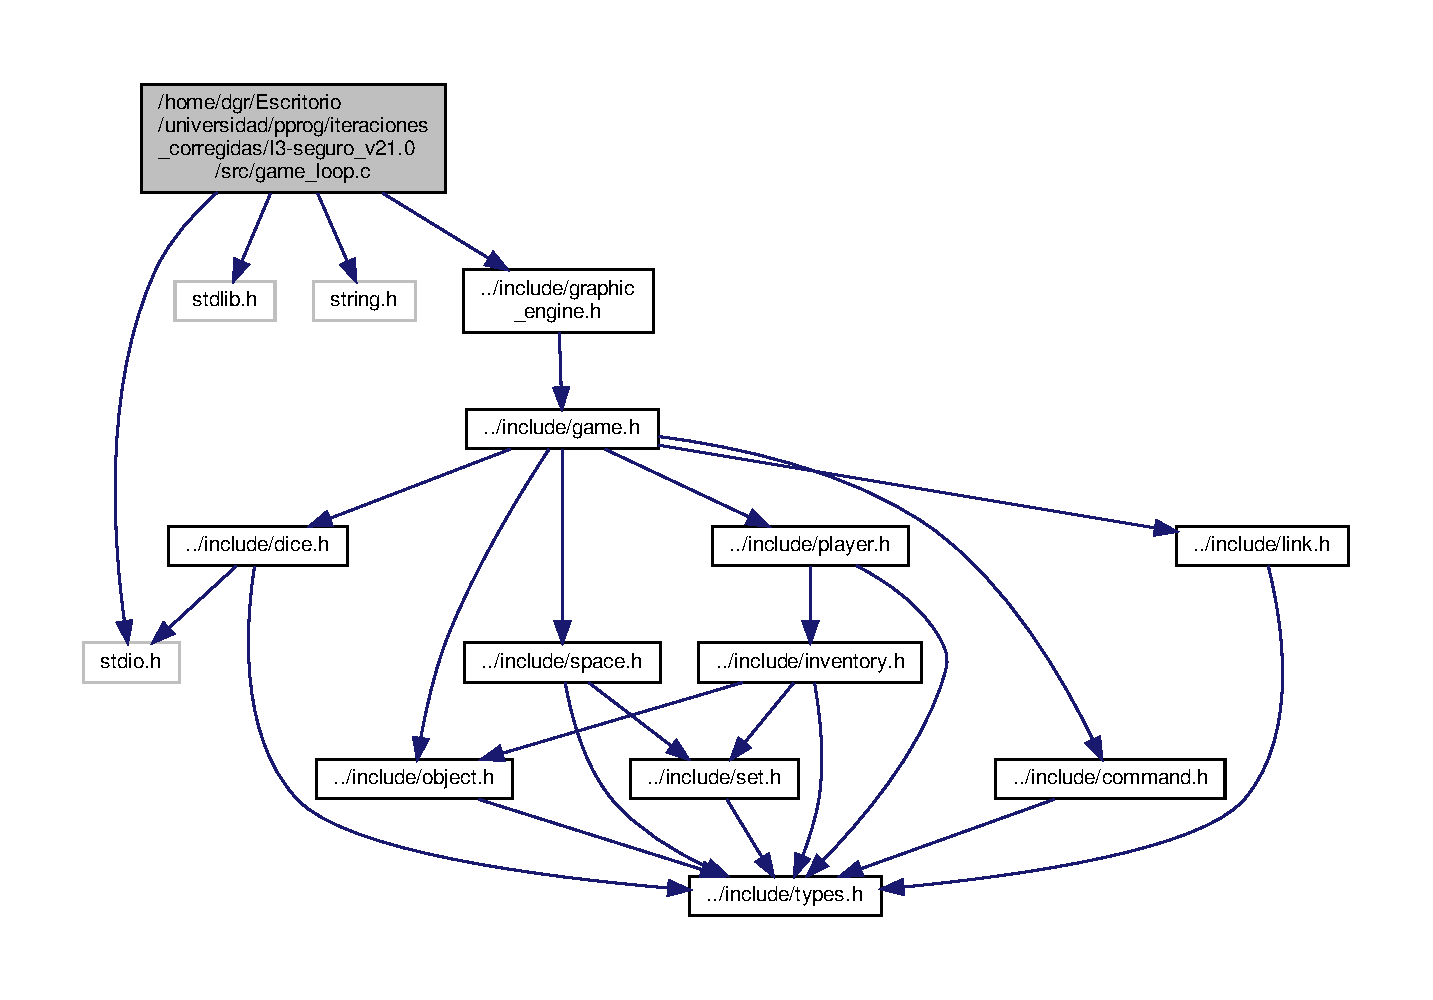
\includegraphics[width=350pt]{game__loop_8c__incl}
\end{center}
\end{figure}
\subsection*{Functions}
\begin{DoxyCompactItemize}
\item 
int \hyperlink{game__loop_8c_a1c78d6052c905d10401d2424b6979772}{game\+\_\+loop\+\_\+init} (\hyperlink{game_8h_a57156d39c530aec3fba3a9dad8c2dc6a}{Game} $\ast$$\ast$game, \hyperlink{graphic__engine_8h_ae1bc5cdbfce93098f066274fdea49af1}{Graphic\+\_\+engine} $\ast$$\ast$gengine, char $\ast$file\+\_\+name)
\begin{DoxyCompactList}\small\item\em Initialize the game gane\+\_\+loop\+\_\+init. \end{DoxyCompactList}\item 
void \hyperlink{game__loop_8c_a49a17889d8305159c4d9e9ffa42ca284}{game\+\_\+loop\+\_\+run} (\hyperlink{game_8h_a57156d39c530aec3fba3a9dad8c2dc6a}{Game} $\ast$game, \hyperlink{graphic__engine_8h_ae1bc5cdbfce93098f066274fdea49af1}{Graphic\+\_\+engine} $\ast$gengine, F\+I\+LE $\ast$file, char $\ast$filename)
\begin{DoxyCompactList}\small\item\em Initialize the game loop game\+\_\+loop\+\_\+run. \end{DoxyCompactList}\item 
void \hyperlink{game__loop_8c_a395965726eadd591bc6c02fed4709a4e}{game\+\_\+loop\+\_\+cleanup} (\hyperlink{game_8h_a57156d39c530aec3fba3a9dad8c2dc6a}{Game} $\ast$game, \hyperlink{graphic__engine_8h_ae1bc5cdbfce93098f066274fdea49af1}{Graphic\+\_\+engine} $\ast$gengine)
\begin{DoxyCompactList}\small\item\em Initialize the Initializes the release of dynamic memory. \end{DoxyCompactList}\item 
int \hyperlink{game__loop_8c_a0ddf1224851353fc92bfbff6f499fa97}{main} (int argc, char $\ast$argv\mbox{[}$\,$\mbox{]})
\begin{DoxyCompactList}\small\item\em the main function of game\+\_\+loop main \end{DoxyCompactList}\end{DoxyCompactItemize}


\subsection{Detailed Description}
It defines the game loop. 

\begin{DoxyAuthor}{Author}
Profesores P\+P\+R\+OG 
\end{DoxyAuthor}
\begin{DoxyVersion}{Version}
1.\+0 
\end{DoxyVersion}
\begin{DoxyDate}{Date}
13-\/01-\/2015 
\end{DoxyDate}
\begin{DoxyCopyright}{Copyright}
G\+NU Public License 
\end{DoxyCopyright}


\subsection{Function Documentation}
\mbox{\Hypertarget{game__loop_8c_a395965726eadd591bc6c02fed4709a4e}\label{game__loop_8c_a395965726eadd591bc6c02fed4709a4e}} 
\index{game\+\_\+loop.\+c@{game\+\_\+loop.\+c}!game\+\_\+loop\+\_\+cleanup@{game\+\_\+loop\+\_\+cleanup}}
\index{game\+\_\+loop\+\_\+cleanup@{game\+\_\+loop\+\_\+cleanup}!game\+\_\+loop.\+c@{game\+\_\+loop.\+c}}
\subsubsection{\texorpdfstring{game\+\_\+loop\+\_\+cleanup()}{game\_loop\_cleanup()}}
{\footnotesize\ttfamily void game\+\_\+loop\+\_\+cleanup (\begin{DoxyParamCaption}\item[{\hyperlink{game_8h_a57156d39c530aec3fba3a9dad8c2dc6a}{Game} $\ast$}]{game,  }\item[{\hyperlink{graphic__engine_8h_ae1bc5cdbfce93098f066274fdea49af1}{Graphic\+\_\+engine} $\ast$}]{gengine }\end{DoxyParamCaption})}



Initialize the Initializes the release of dynamic memory. 

\begin{DoxyDate}{Date}
10/02/2020 
\end{DoxyDate}
\begin{DoxyAuthor}{Author}
\+: Profesores P\+P\+R\+OG
\end{DoxyAuthor}

\begin{DoxyParams}{Parameters}
{\em game} & game address \\
\hline
{\em gengine} & $\ast$gengine address \\
\hline
\end{DoxyParams}
\begin{DoxyReturn}{Returns}

\end{DoxyReturn}
\mbox{\Hypertarget{game__loop_8c_a1c78d6052c905d10401d2424b6979772}\label{game__loop_8c_a1c78d6052c905d10401d2424b6979772}} 
\index{game\+\_\+loop.\+c@{game\+\_\+loop.\+c}!game\+\_\+loop\+\_\+init@{game\+\_\+loop\+\_\+init}}
\index{game\+\_\+loop\+\_\+init@{game\+\_\+loop\+\_\+init}!game\+\_\+loop.\+c@{game\+\_\+loop.\+c}}
\subsubsection{\texorpdfstring{game\+\_\+loop\+\_\+init()}{game\_loop\_init()}}
{\footnotesize\ttfamily int game\+\_\+loop\+\_\+init (\begin{DoxyParamCaption}\item[{\hyperlink{game_8h_a57156d39c530aec3fba3a9dad8c2dc6a}{Game} $\ast$$\ast$}]{game,  }\item[{\hyperlink{graphic__engine_8h_ae1bc5cdbfce93098f066274fdea49af1}{Graphic\+\_\+engine} $\ast$$\ast$}]{gengine,  }\item[{char $\ast$}]{file\+\_\+name }\end{DoxyParamCaption})}



Initialize the game gane\+\_\+loop\+\_\+init. 

\begin{DoxyDate}{Date}
10/02/2020 
\end{DoxyDate}
\begin{DoxyAuthor}{Author}
\+: Profesores P\+P\+R\+OG
\end{DoxyAuthor}

\begin{DoxyParams}{Parameters}
{\em game} & game address \\
\hline
{\em gengine} & $\ast$gengine address \\
\hline
{\em file\+\_\+name} & file name addres \\
\hline
\end{DoxyParams}
\begin{DoxyReturn}{Returns}
Returns 0 or 1 in case of error 
\end{DoxyReturn}
\mbox{\Hypertarget{game__loop_8c_a49a17889d8305159c4d9e9ffa42ca284}\label{game__loop_8c_a49a17889d8305159c4d9e9ffa42ca284}} 
\index{game\+\_\+loop.\+c@{game\+\_\+loop.\+c}!game\+\_\+loop\+\_\+run@{game\+\_\+loop\+\_\+run}}
\index{game\+\_\+loop\+\_\+run@{game\+\_\+loop\+\_\+run}!game\+\_\+loop.\+c@{game\+\_\+loop.\+c}}
\subsubsection{\texorpdfstring{game\+\_\+loop\+\_\+run()}{game\_loop\_run()}}
{\footnotesize\ttfamily void game\+\_\+loop\+\_\+run (\begin{DoxyParamCaption}\item[{\hyperlink{game_8h_a57156d39c530aec3fba3a9dad8c2dc6a}{Game} $\ast$}]{game,  }\item[{\hyperlink{graphic__engine_8h_ae1bc5cdbfce93098f066274fdea49af1}{Graphic\+\_\+engine} $\ast$}]{gengine,  }\item[{F\+I\+LE $\ast$}]{file,  }\item[{char $\ast$}]{filename }\end{DoxyParamCaption})}



Initialize the game loop game\+\_\+loop\+\_\+run. 

\begin{DoxyDate}{Date}
10/02/2020 
\end{DoxyDate}
\begin{DoxyAuthor}{Author}
\+: Profesores P\+P\+R\+OG
\end{DoxyAuthor}

\begin{DoxyParams}{Parameters}
{\em game} & game address \\
\hline
{\em gengine} & gengine address \\
\hline
{\em file} & file address \\
\hline
{\em filename} & the name of the file \\
\hline
\end{DoxyParams}
\begin{DoxyReturn}{Returns}

\end{DoxyReturn}
\mbox{\Hypertarget{game__loop_8c_a0ddf1224851353fc92bfbff6f499fa97}\label{game__loop_8c_a0ddf1224851353fc92bfbff6f499fa97}} 
\index{game\+\_\+loop.\+c@{game\+\_\+loop.\+c}!main@{main}}
\index{main@{main}!game\+\_\+loop.\+c@{game\+\_\+loop.\+c}}
\subsubsection{\texorpdfstring{main()}{main()}}
{\footnotesize\ttfamily int main (\begin{DoxyParamCaption}\item[{int}]{argc,  }\item[{char $\ast$}]{argv\mbox{[}$\,$\mbox{]} }\end{DoxyParamCaption})}



the main function of game\+\_\+loop main 

\begin{DoxyDate}{Date}
06-\/03-\/2019 
\end{DoxyDate}
\begin{DoxyAuthor}{Author}
Instructor of P\+P\+R\+OG 
\end{DoxyAuthor}

\begin{DoxyParams}{Parameters}
{\em argc} & number received at start of run \\
\hline
{\em argv} & array of strings received at start of run \\
\hline
\end{DoxyParams}
\begin{DoxyReturn}{Returns}

\end{DoxyReturn}

\hypertarget{inventory_8c}{}\section{src/inventory.c File Reference}
\label{inventory_8c}\index{src/inventory.\+c@{src/inventory.\+c}}


It implements the inventory interpreter.  


{\ttfamily \#include $<$stdio.\+h$>$}\newline
{\ttfamily \#include $<$stdlib.\+h$>$}\newline
{\ttfamily \#include \char`\"{}../include/inventory.\+h\char`\"{}}\newline
Include dependency graph for inventory.\+c\+:\nopagebreak
\begin{figure}[H]
\begin{center}
\leavevmode
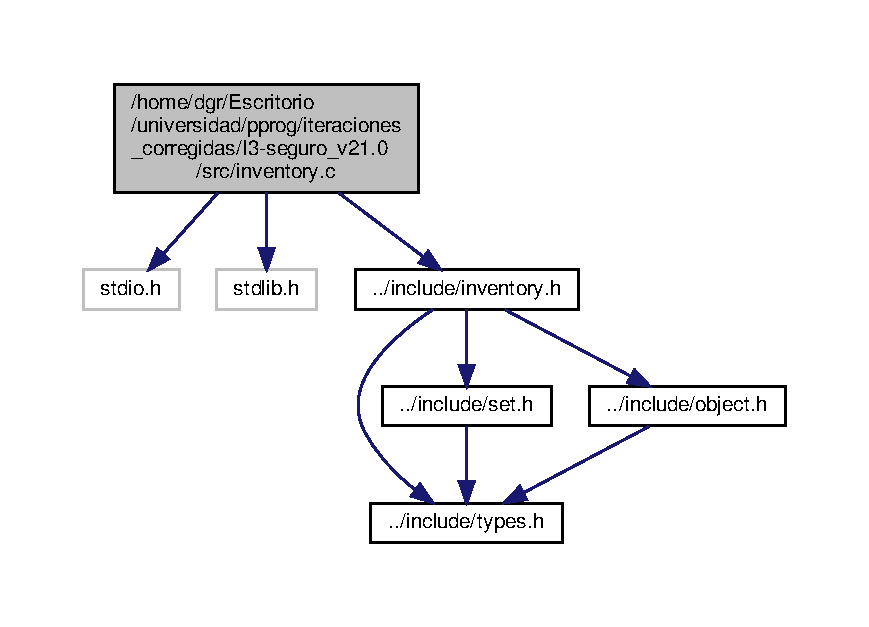
\includegraphics[width=340pt]{inventory_8c__incl}
\end{center}
\end{figure}
\subsection*{Data Structures}
\begin{DoxyCompactItemize}
\item 
struct \hyperlink{struct__Inventory}{\+\_\+\+Inventory}
\begin{DoxyCompactList}\small\item\em The inventory structure. \end{DoxyCompactList}\end{DoxyCompactItemize}
\subsection*{Functions}
\begin{DoxyCompactItemize}
\item 
\hyperlink{inventory_8h_a2253bf64ac4ce6a9c1d6f39c0b0d32a3}{Inventory} $\ast$ \hyperlink{inventory_8c_a84f90137d8559068d8292b8d10c675a1}{inventory\+\_\+create} (\hyperlink{types_8h_a845e604fb28f7e3d97549da3448149d3}{Id} id, int max)
\begin{DoxyCompactList}\small\item\em Create the inventory. \end{DoxyCompactList}\item 
\hyperlink{types_8h_a32c27cc471df37f4fc818d65de0a56c4}{S\+T\+A\+T\+US} \hyperlink{inventory_8c_a690c5b171251c27a628f0ecaaaf6b9ce}{inventory\+\_\+destroy} (\hyperlink{inventory_8h_a2253bf64ac4ce6a9c1d6f39c0b0d32a3}{Inventory} $\ast$inventory)
\begin{DoxyCompactList}\small\item\em Destroy the inventory. \end{DoxyCompactList}\item 
\hyperlink{set_8h_a6d3b7f7c92cbb4577ef3ef7ddbf93161}{Set} $\ast$ \hyperlink{inventory_8c_a6a1f9cdbffc20d4283f09635c98ffb83}{inventory\+\_\+get\+\_\+inside} (\hyperlink{inventory_8h_a2253bf64ac4ce6a9c1d6f39c0b0d32a3}{Inventory} $\ast$inventory)
\begin{DoxyCompactList}\small\item\em Return the set of the inventory. \end{DoxyCompactList}\item 
\hyperlink{types_8h_a32c27cc471df37f4fc818d65de0a56c4}{S\+T\+A\+T\+US} \hyperlink{inventory_8c_a4f3b96537e64ffc63731555e116c3adb}{inventory\+\_\+add} (\hyperlink{inventory_8h_a2253bf64ac4ce6a9c1d6f39c0b0d32a3}{Inventory} $\ast$inventory, \hyperlink{types_8h_a845e604fb28f7e3d97549da3448149d3}{Id} id)
\begin{DoxyCompactList}\small\item\em Add the object to the inventory. \end{DoxyCompactList}\item 
\hyperlink{types_8h_a32c27cc471df37f4fc818d65de0a56c4}{S\+T\+A\+T\+US} \hyperlink{inventory_8c_a348efe95855b9ecad72ea3b6bf1ce8c4}{inventory\+\_\+dell} (\hyperlink{inventory_8h_a2253bf64ac4ce6a9c1d6f39c0b0d32a3}{Inventory} $\ast$inventory, \hyperlink{types_8h_a845e604fb28f7e3d97549da3448149d3}{Id} id)
\begin{DoxyCompactList}\small\item\em Delete the object of the inventory. \end{DoxyCompactList}\item 
void \hyperlink{inventory_8c_ad5b213ff8ab4ee5f6654cfe9d0107ea2}{inventory\+\_\+print} (F\+I\+LE $\ast$f, \hyperlink{inventory_8h_a2253bf64ac4ce6a9c1d6f39c0b0d32a3}{Inventory} $\ast$inventory)
\begin{DoxyCompactList}\small\item\em Print the inventory and on a file given. \end{DoxyCompactList}\item 
\hyperlink{types_8h_a3e5b8192e7d9ffaf3542f1210aec18dd}{B\+O\+OL} \hyperlink{inventory_8c_a7da45e3f52165fd1e3a51c95aa6f78f8}{inventory\+\_\+is\+\_\+object} (\hyperlink{inventory_8h_a2253bf64ac4ce6a9c1d6f39c0b0d32a3}{Inventory} $\ast$inventory, \hyperlink{types_8h_a845e604fb28f7e3d97549da3448149d3}{Id} id)
\begin{DoxyCompactList}\small\item\em check if the object is in inventory \end{DoxyCompactList}\item 
int \hyperlink{inventory_8c_aac41dfbea9df9fcfbbebfec318ddd636}{inventory\+\_\+get\+\_\+max} (\hyperlink{inventory_8h_a2253bf64ac4ce6a9c1d6f39c0b0d32a3}{Inventory} $\ast$inventory)
\begin{DoxyCompactList}\small\item\em return the max number of objects of an inventory \end{DoxyCompactList}\item 
\hyperlink{types_8h_a3e5b8192e7d9ffaf3542f1210aec18dd}{B\+O\+OL} \hyperlink{inventory_8c_a31ce870d22db2381928f052c77b28288}{inventory\+\_\+is\+\_\+full} (\hyperlink{inventory_8h_a2253bf64ac4ce6a9c1d6f39c0b0d32a3}{Inventory} $\ast$inventory)
\begin{DoxyCompactList}\small\item\em check if the inventory is full \end{DoxyCompactList}\item 
\hyperlink{types_8h_a3e5b8192e7d9ffaf3542f1210aec18dd}{B\+O\+OL} \hyperlink{inventory_8c_a5be8b836d5bb5a948aab616ef404b1cd}{inventory\+\_\+is\+\_\+emty} (\hyperlink{inventory_8h_a2253bf64ac4ce6a9c1d6f39c0b0d32a3}{Inventory} $\ast$inventory)
\begin{DoxyCompactList}\small\item\em check if the inventory is empty \end{DoxyCompactList}\item 
\hyperlink{types_8h_a845e604fb28f7e3d97549da3448149d3}{Id} \hyperlink{inventory_8c_ae8ad5fa7c6e871a8fe03f6e7a54b05cc}{inventory\+\_\+get\+\_\+id} (\hyperlink{inventory_8h_a2253bf64ac4ce6a9c1d6f39c0b0d32a3}{Inventory} $\ast$inv)
\begin{DoxyCompactList}\small\item\em Print the inventory and on a file given. \end{DoxyCompactList}\end{DoxyCompactItemize}


\subsection{Detailed Description}
It implements the inventory interpreter. 

\begin{DoxyAuthor}{Author}
Profesores P\+P\+R\+OG 
\end{DoxyAuthor}
\begin{DoxyVersion}{Version}
2.\+0 
\end{DoxyVersion}
\begin{DoxyDate}{Date}
10-\/01-\/2020 
\end{DoxyDate}
\begin{DoxyCopyright}{Copyright}
G\+NU Public License 
\end{DoxyCopyright}


\subsection{Function Documentation}
\mbox{\Hypertarget{inventory_8c_a4f3b96537e64ffc63731555e116c3adb}\label{inventory_8c_a4f3b96537e64ffc63731555e116c3adb}} 
\index{inventory.\+c@{inventory.\+c}!inventory\+\_\+add@{inventory\+\_\+add}}
\index{inventory\+\_\+add@{inventory\+\_\+add}!inventory.\+c@{inventory.\+c}}
\subsubsection{\texorpdfstring{inventory\+\_\+add()}{inventory\_add()}}
{\footnotesize\ttfamily \hyperlink{types_8h_a32c27cc471df37f4fc818d65de0a56c4}{S\+T\+A\+T\+US} inventory\+\_\+add (\begin{DoxyParamCaption}\item[{\hyperlink{inventory_8h_a2253bf64ac4ce6a9c1d6f39c0b0d32a3}{Inventory} $\ast$}]{inventory,  }\item[{\hyperlink{types_8h_a845e604fb28f7e3d97549da3448149d3}{Id}}]{id }\end{DoxyParamCaption})}



Add the object to the inventory. 

\begin{DoxyDate}{Date}
14-\/03-\/2020 
\end{DoxyDate}
\begin{DoxyAuthor}{Author}
\+: Diego Grande Camarero
\end{DoxyAuthor}

\begin{DoxyParams}{Parameters}
{\em inventory} & Pointer to the inventory \\
\hline
{\em id} & The object id \\
\hline
\end{DoxyParams}
\begin{DoxyReturn}{Returns}
Ok if there was no problem, E\+R\+R\+OR if not 
\end{DoxyReturn}
\mbox{\Hypertarget{inventory_8c_a84f90137d8559068d8292b8d10c675a1}\label{inventory_8c_a84f90137d8559068d8292b8d10c675a1}} 
\index{inventory.\+c@{inventory.\+c}!inventory\+\_\+create@{inventory\+\_\+create}}
\index{inventory\+\_\+create@{inventory\+\_\+create}!inventory.\+c@{inventory.\+c}}
\subsubsection{\texorpdfstring{inventory\+\_\+create()}{inventory\_create()}}
{\footnotesize\ttfamily \hyperlink{inventory_8h_a2253bf64ac4ce6a9c1d6f39c0b0d32a3}{Inventory}$\ast$ inventory\+\_\+create (\begin{DoxyParamCaption}\item[{\hyperlink{types_8h_a845e604fb28f7e3d97549da3448149d3}{Id}}]{id,  }\item[{int}]{max }\end{DoxyParamCaption})}



Create the inventory. 

inventory\+\_\+create Create a new inventory

\begin{DoxyDate}{Date}
14-\/03-\/2020 
\end{DoxyDate}
\begin{DoxyAuthor}{Author}
\+: Diego Grande Camarero
\end{DoxyAuthor}

\begin{DoxyParams}{Parameters}
{\em id} & id of the inventory \\
\hline
{\em max} & max number of objects it will contain \\
\hline
\end{DoxyParams}
\begin{DoxyReturn}{Returns}
the new inventory that has been created 
\end{DoxyReturn}
\mbox{\Hypertarget{inventory_8c_a348efe95855b9ecad72ea3b6bf1ce8c4}\label{inventory_8c_a348efe95855b9ecad72ea3b6bf1ce8c4}} 
\index{inventory.\+c@{inventory.\+c}!inventory\+\_\+dell@{inventory\+\_\+dell}}
\index{inventory\+\_\+dell@{inventory\+\_\+dell}!inventory.\+c@{inventory.\+c}}
\subsubsection{\texorpdfstring{inventory\+\_\+dell()}{inventory\_dell()}}
{\footnotesize\ttfamily \hyperlink{types_8h_a32c27cc471df37f4fc818d65de0a56c4}{S\+T\+A\+T\+US} inventory\+\_\+dell (\begin{DoxyParamCaption}\item[{\hyperlink{inventory_8h_a2253bf64ac4ce6a9c1d6f39c0b0d32a3}{Inventory} $\ast$}]{inventory,  }\item[{\hyperlink{types_8h_a845e604fb28f7e3d97549da3448149d3}{Id}}]{id }\end{DoxyParamCaption})}



Delete the object of the inventory. 

\begin{DoxyDate}{Date}
14-\/03-\/2020 
\end{DoxyDate}
\begin{DoxyAuthor}{Author}
Diego Grande Camarero
\end{DoxyAuthor}

\begin{DoxyParams}{Parameters}
{\em inventory} & Pointer to the inventory \\
\hline
{\em id} & id of the object \\
\hline
\end{DoxyParams}
\begin{DoxyReturn}{Returns}
Ok if there was no problem, E\+R\+R\+OR if not 
\end{DoxyReturn}
\mbox{\Hypertarget{inventory_8c_a690c5b171251c27a628f0ecaaaf6b9ce}\label{inventory_8c_a690c5b171251c27a628f0ecaaaf6b9ce}} 
\index{inventory.\+c@{inventory.\+c}!inventory\+\_\+destroy@{inventory\+\_\+destroy}}
\index{inventory\+\_\+destroy@{inventory\+\_\+destroy}!inventory.\+c@{inventory.\+c}}
\subsubsection{\texorpdfstring{inventory\+\_\+destroy()}{inventory\_destroy()}}
{\footnotesize\ttfamily \hyperlink{types_8h_a32c27cc471df37f4fc818d65de0a56c4}{S\+T\+A\+T\+US} inventory\+\_\+destroy (\begin{DoxyParamCaption}\item[{\hyperlink{inventory_8h_a2253bf64ac4ce6a9c1d6f39c0b0d32a3}{Inventory} $\ast$}]{inventory }\end{DoxyParamCaption})}



Destroy the inventory. 

inventory\+\_\+destroy Destroy the inventory

\begin{DoxyDate}{Date}
14-\/03-\/2020 
\end{DoxyDate}
\begin{DoxyAuthor}{Author}
Diego Grande Camarero
\end{DoxyAuthor}

\begin{DoxyParams}{Parameters}
{\em inventory} & Pointer to the inventory \\
\hline
\end{DoxyParams}
\begin{DoxyReturn}{Returns}
Ok if the inventory has been destroyed 
\end{DoxyReturn}
\mbox{\Hypertarget{inventory_8c_ae8ad5fa7c6e871a8fe03f6e7a54b05cc}\label{inventory_8c_ae8ad5fa7c6e871a8fe03f6e7a54b05cc}} 
\index{inventory.\+c@{inventory.\+c}!inventory\+\_\+get\+\_\+id@{inventory\+\_\+get\+\_\+id}}
\index{inventory\+\_\+get\+\_\+id@{inventory\+\_\+get\+\_\+id}!inventory.\+c@{inventory.\+c}}
\subsubsection{\texorpdfstring{inventory\+\_\+get\+\_\+id()}{inventory\_get\_id()}}
{\footnotesize\ttfamily \hyperlink{types_8h_a845e604fb28f7e3d97549da3448149d3}{Id} inventory\+\_\+get\+\_\+id (\begin{DoxyParamCaption}\item[{\hyperlink{inventory_8h_a2253bf64ac4ce6a9c1d6f39c0b0d32a3}{Inventory} $\ast$}]{inv }\end{DoxyParamCaption})}



Print the inventory and on a file given. 

\begin{DoxyDate}{Date}
14-\/05-\/2020 
\end{DoxyDate}
\begin{DoxyAuthor}{Author}
David Teófilo Garitagoiria Romero
\end{DoxyAuthor}

\begin{DoxyParams}{Parameters}
{\em inv} & pointer to the inventory \\
\hline
\end{DoxyParams}
\begin{DoxyReturn}{Returns}
the id of the inventory 
\end{DoxyReturn}
\mbox{\Hypertarget{inventory_8c_a6a1f9cdbffc20d4283f09635c98ffb83}\label{inventory_8c_a6a1f9cdbffc20d4283f09635c98ffb83}} 
\index{inventory.\+c@{inventory.\+c}!inventory\+\_\+get\+\_\+inside@{inventory\+\_\+get\+\_\+inside}}
\index{inventory\+\_\+get\+\_\+inside@{inventory\+\_\+get\+\_\+inside}!inventory.\+c@{inventory.\+c}}
\subsubsection{\texorpdfstring{inventory\+\_\+get\+\_\+inside()}{inventory\_get\_inside()}}
{\footnotesize\ttfamily \hyperlink{set_8h_a6d3b7f7c92cbb4577ef3ef7ddbf93161}{Set}$\ast$ inventory\+\_\+get\+\_\+inside (\begin{DoxyParamCaption}\item[{\hyperlink{inventory_8h_a2253bf64ac4ce6a9c1d6f39c0b0d32a3}{Inventory} $\ast$}]{inventory }\end{DoxyParamCaption})}



Return the set of the inventory. 

\begin{DoxyDate}{Date}
14-\/03-\/2020 
\end{DoxyDate}
\begin{DoxyAuthor}{Author}
\+: David Teófilo Garitagoitia Romero
\end{DoxyAuthor}

\begin{DoxyParams}{Parameters}
{\em inventory} & Pointer to the inventory \\
\hline
\end{DoxyParams}
\begin{DoxyReturn}{Returns}
Ok if there was no problem, E\+R\+R\+OR if not 
\end{DoxyReturn}
\mbox{\Hypertarget{inventory_8c_aac41dfbea9df9fcfbbebfec318ddd636}\label{inventory_8c_aac41dfbea9df9fcfbbebfec318ddd636}} 
\index{inventory.\+c@{inventory.\+c}!inventory\+\_\+get\+\_\+max@{inventory\+\_\+get\+\_\+max}}
\index{inventory\+\_\+get\+\_\+max@{inventory\+\_\+get\+\_\+max}!inventory.\+c@{inventory.\+c}}
\subsubsection{\texorpdfstring{inventory\+\_\+get\+\_\+max()}{inventory\_get\_max()}}
{\footnotesize\ttfamily int inventory\+\_\+get\+\_\+max (\begin{DoxyParamCaption}\item[{\hyperlink{inventory_8h_a2253bf64ac4ce6a9c1d6f39c0b0d32a3}{Inventory} $\ast$}]{inventory }\end{DoxyParamCaption})}



return the max number of objects of an inventory 

\begin{DoxyDate}{Date}
14-\/03-\/2020 
\end{DoxyDate}
\begin{DoxyAuthor}{Author}
\+: David Teófilo Garitagoitia Romero
\end{DoxyAuthor}

\begin{DoxyParams}{Parameters}
{\em inventory} & Pointer to the inventory \\
\hline
\end{DoxyParams}
\begin{DoxyReturn}{Returns}
the max number of objects of an inventory 
\end{DoxyReturn}
\mbox{\Hypertarget{inventory_8c_a5be8b836d5bb5a948aab616ef404b1cd}\label{inventory_8c_a5be8b836d5bb5a948aab616ef404b1cd}} 
\index{inventory.\+c@{inventory.\+c}!inventory\+\_\+is\+\_\+emty@{inventory\+\_\+is\+\_\+emty}}
\index{inventory\+\_\+is\+\_\+emty@{inventory\+\_\+is\+\_\+emty}!inventory.\+c@{inventory.\+c}}
\subsubsection{\texorpdfstring{inventory\+\_\+is\+\_\+emty()}{inventory\_is\_emty()}}
{\footnotesize\ttfamily \hyperlink{types_8h_a3e5b8192e7d9ffaf3542f1210aec18dd}{B\+O\+OL} inventory\+\_\+is\+\_\+emty (\begin{DoxyParamCaption}\item[{\hyperlink{inventory_8h_a2253bf64ac4ce6a9c1d6f39c0b0d32a3}{Inventory} $\ast$}]{inventory }\end{DoxyParamCaption})}



check if the inventory is empty 

\begin{DoxyDate}{Date}
14-\/03-\/2020 
\end{DoxyDate}
\begin{DoxyAuthor}{Author}
\+: David Teófilo Garitagoitia Romero
\end{DoxyAuthor}

\begin{DoxyParams}{Parameters}
{\em inventory} & Pointer to the inventory \\
\hline
\end{DoxyParams}
\begin{DoxyReturn}{Returns}
true in case that the inventory is empty, false otherwise 
\end{DoxyReturn}
\mbox{\Hypertarget{inventory_8c_a31ce870d22db2381928f052c77b28288}\label{inventory_8c_a31ce870d22db2381928f052c77b28288}} 
\index{inventory.\+c@{inventory.\+c}!inventory\+\_\+is\+\_\+full@{inventory\+\_\+is\+\_\+full}}
\index{inventory\+\_\+is\+\_\+full@{inventory\+\_\+is\+\_\+full}!inventory.\+c@{inventory.\+c}}
\subsubsection{\texorpdfstring{inventory\+\_\+is\+\_\+full()}{inventory\_is\_full()}}
{\footnotesize\ttfamily \hyperlink{types_8h_a3e5b8192e7d9ffaf3542f1210aec18dd}{B\+O\+OL} inventory\+\_\+is\+\_\+full (\begin{DoxyParamCaption}\item[{\hyperlink{inventory_8h_a2253bf64ac4ce6a9c1d6f39c0b0d32a3}{Inventory} $\ast$}]{inventory }\end{DoxyParamCaption})}



check if the inventory is full 

\begin{DoxyDate}{Date}
14-\/03-\/2020 
\end{DoxyDate}
\begin{DoxyAuthor}{Author}
\+: David Teófilo Garitagoitia Romero
\end{DoxyAuthor}

\begin{DoxyParams}{Parameters}
{\em inventory} & Pointer to the inventory \\
\hline
\end{DoxyParams}
\begin{DoxyReturn}{Returns}
true in case that the inventory is full, false otherwise 
\end{DoxyReturn}
\mbox{\Hypertarget{inventory_8c_a7da45e3f52165fd1e3a51c95aa6f78f8}\label{inventory_8c_a7da45e3f52165fd1e3a51c95aa6f78f8}} 
\index{inventory.\+c@{inventory.\+c}!inventory\+\_\+is\+\_\+object@{inventory\+\_\+is\+\_\+object}}
\index{inventory\+\_\+is\+\_\+object@{inventory\+\_\+is\+\_\+object}!inventory.\+c@{inventory.\+c}}
\subsubsection{\texorpdfstring{inventory\+\_\+is\+\_\+object()}{inventory\_is\_object()}}
{\footnotesize\ttfamily \hyperlink{types_8h_a3e5b8192e7d9ffaf3542f1210aec18dd}{B\+O\+OL} inventory\+\_\+is\+\_\+object (\begin{DoxyParamCaption}\item[{\hyperlink{inventory_8h_a2253bf64ac4ce6a9c1d6f39c0b0d32a3}{Inventory} $\ast$}]{inventory,  }\item[{\hyperlink{types_8h_a845e604fb28f7e3d97549da3448149d3}{Id}}]{id }\end{DoxyParamCaption})}



check if the object is in inventory 

\begin{DoxyDate}{Date}
14-\/03-\/2020 
\end{DoxyDate}
\begin{DoxyAuthor}{Author}
\+: David Teófilo Garitagoitia Romero
\end{DoxyAuthor}

\begin{DoxyParams}{Parameters}
{\em inventory} & Pointer to the inventory \\
\hline
{\em id} & Id of the object \\
\hline
\end{DoxyParams}
\begin{DoxyReturn}{Returns}
True if the object is in the inventory, false otherwise 
\end{DoxyReturn}
\mbox{\Hypertarget{inventory_8c_ad5b213ff8ab4ee5f6654cfe9d0107ea2}\label{inventory_8c_ad5b213ff8ab4ee5f6654cfe9d0107ea2}} 
\index{inventory.\+c@{inventory.\+c}!inventory\+\_\+print@{inventory\+\_\+print}}
\index{inventory\+\_\+print@{inventory\+\_\+print}!inventory.\+c@{inventory.\+c}}
\subsubsection{\texorpdfstring{inventory\+\_\+print()}{inventory\_print()}}
{\footnotesize\ttfamily void inventory\+\_\+print (\begin{DoxyParamCaption}\item[{F\+I\+LE $\ast$}]{f,  }\item[{\hyperlink{inventory_8h_a2253bf64ac4ce6a9c1d6f39c0b0d32a3}{Inventory} $\ast$}]{inventory }\end{DoxyParamCaption})}



Print the inventory and on a file given. 

\begin{DoxyDate}{Date}
14-\/03-\/2020 
\end{DoxyDate}
\begin{DoxyAuthor}{Author}
Diego Grande Camarero
\end{DoxyAuthor}

\begin{DoxyParams}{Parameters}
{\em f} & Pointer to the file \\
\hline
{\em inventory} & pointer to the inventory \\
\hline
\end{DoxyParams}
\begin{DoxyReturn}{Returns}

\end{DoxyReturn}

\hypertarget{inventory__test_8c}{}\section{/home/dgr/\+Escritorio/universidad/pprog/iteraciones\+\_\+corregidas/\+I3-\/seguro\+\_\+v21.0/src/inventory\+\_\+test.c File Reference}
\label{inventory__test_8c}\index{/home/dgr/\+Escritorio/universidad/pprog/iteraciones\+\_\+corregidas/\+I3-\/seguro\+\_\+v21.\+0/src/inventory\+\_\+test.\+c@{/home/dgr/\+Escritorio/universidad/pprog/iteraciones\+\_\+corregidas/\+I3-\/seguro\+\_\+v21.\+0/src/inventory\+\_\+test.\+c}}


test to see if inventory works correctly  


{\ttfamily \#include $<$stdio.\+h$>$}\newline
{\ttfamily \#include $<$string.\+h$>$}\newline
{\ttfamily \#include $<$stdlib.\+h$>$}\newline
{\ttfamily \#include \char`\"{}../include/inventory.\+h\char`\"{}}\newline
{\ttfamily \#include \char`\"{}../include/test.\+h\char`\"{}}\newline
{\ttfamily \#include \char`\"{}../include/inventory\+\_\+test.\+h\char`\"{}}\newline
Include dependency graph for inventory\+\_\+test.\+c\+:
\nopagebreak
\begin{figure}[H]
\begin{center}
\leavevmode
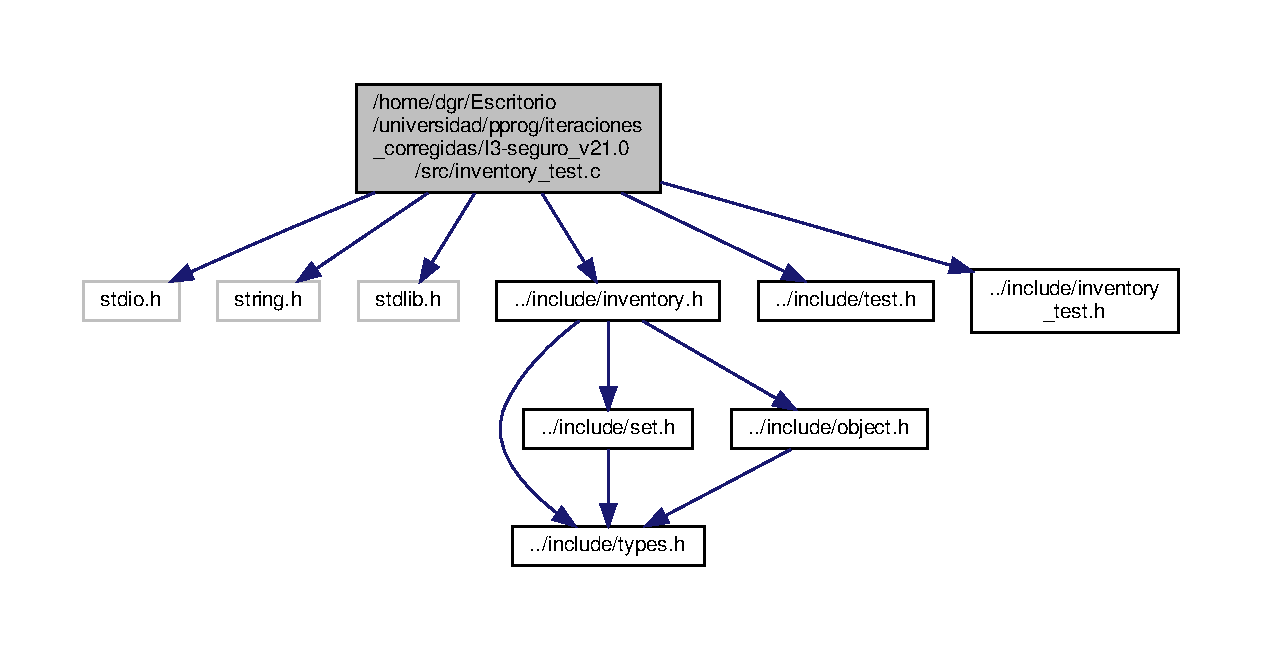
\includegraphics[width=350pt]{inventory__test_8c__incl}
\end{center}
\end{figure}
\subsection*{Macros}
\begin{DoxyCompactItemize}
\item 
\#define \hyperlink{inventory__test_8c_a2a77d2f2c5b698c69c19e1f8782bf709}{M\+A\+X\+\_\+\+T\+E\+S\+TS}~24
\begin{DoxyCompactList}\small\item\em maximum number of test \end{DoxyCompactList}\end{DoxyCompactItemize}
\subsection*{Functions}
\begin{DoxyCompactItemize}
\item 
int \hyperlink{inventory__test_8c_a3c04138a5bfe5d72780bb7e82a18e627}{main} (int argc, char $\ast$$\ast$argv)
\begin{DoxyCompactList}\small\item\em the main function of inventory\+\_\+test main \end{DoxyCompactList}\item 
void \hyperlink{inventory__test_8c_a33638f1a88ae16ab8d6bee00145b82b8}{test1\+\_\+inventory\+\_\+create} ()
\item 
void \hyperlink{inventory__test_8c_a73a6080c360a8870c4ffc734e989c8b3}{test2\+\_\+inventory\+\_\+create} ()
\item 
void \hyperlink{inventory__test_8c_ad8c004bf0a89d5559e5135a0e0096734}{test1\+\_\+inventory\+\_\+get\+\_\+inside} ()
\item 
void \hyperlink{inventory__test_8c_aa90dc9b98c6d00cbb1fd8be85f9be762}{test2\+\_\+inventory\+\_\+get\+\_\+inside} ()
\item 
void \hyperlink{inventory__test_8c_ae81ec4669af03331ca8a228567736474}{test1\+\_\+inventory\+\_\+add} ()
\item 
void \hyperlink{inventory__test_8c_a48019cb45cb5918233d5d42334d2be17}{test2\+\_\+inventory\+\_\+add} ()
\item 
void \hyperlink{inventory__test_8c_ada5ad194dfe9af537c6b2805bf38910d}{test3\+\_\+inventory\+\_\+add} ()
\item 
void \hyperlink{inventory__test_8c_ac67b0f65fccde3f078e6df452e21cee5}{test1\+\_\+inventory\+\_\+dell} ()
\item 
void \hyperlink{inventory__test_8c_ac0175a02211c4bb5ecffbb9f0ebd1152}{test2\+\_\+inventory\+\_\+dell} ()
\item 
void \hyperlink{inventory__test_8c_a030d6ca8db55a616fe0804b3d0c0c144}{test3\+\_\+inventory\+\_\+dell} ()
\item 
void \hyperlink{inventory__test_8c_a19a0bada9e0ce0def239c2b9523ccfea}{test1\+\_\+inventory\+\_\+is\+\_\+object} ()
\item 
void \hyperlink{inventory__test_8c_a7dc6f9e65941e8cf9b6a983a0de7fc5a}{test2\+\_\+inventory\+\_\+is\+\_\+object} ()
\item 
void \hyperlink{inventory__test_8c_a3adf29b420e3d91803c1dd71f374b468}{test3\+\_\+inventory\+\_\+is\+\_\+object} ()
\item 
void \hyperlink{inventory__test_8c_a257dbc0f18af4e4f73163014faa0783a}{test4\+\_\+inventory\+\_\+is\+\_\+object} ()
\item 
void \hyperlink{inventory__test_8c_a17c03f02b989bb00b04155c12fe2af9d}{test1\+\_\+inventory\+\_\+get\+\_\+max} ()
\item 
void \hyperlink{inventory__test_8c_abddcab377edb21235d6746668597fde2}{test2\+\_\+inventory\+\_\+get\+\_\+max} ()
\item 
void \hyperlink{inventory__test_8c_a7eb3ba387e33c42ff45331c9d9aada34}{test1\+\_\+inventory\+\_\+is\+\_\+full} ()
\item 
void \hyperlink{inventory__test_8c_a1c9e567d4919d5aaccc9580815a8a81d}{test2\+\_\+inventory\+\_\+is\+\_\+full} ()
\item 
void \hyperlink{inventory__test_8c_a540dbcbfd29bd63590d081e496f8227f}{test3\+\_\+inventory\+\_\+is\+\_\+full} ()
\item 
void \hyperlink{inventory__test_8c_a0bfdf05239ed2dbac84e7c1240d27de3}{test1\+\_\+inventory\+\_\+is\+\_\+emty} ()
\item 
void \hyperlink{inventory__test_8c_a00a4e952d7b94aedfdac9bb07ec53b0a}{test2\+\_\+inventory\+\_\+is\+\_\+emty} ()
\item 
void \hyperlink{inventory__test_8c_a8cf624674fe17e81eedcb5801f106016}{test3\+\_\+inventory\+\_\+is\+\_\+emty} ()
\item 
void \hyperlink{inventory__test_8c_ab9578e8992c9afab849de87a6f5e637a}{test1\+\_\+inventory\+\_\+get\+\_\+id} ()
\item 
void \hyperlink{inventory__test_8c_ae39f02e7d91f78fabb2faaa4c3b4f7a7}{test2\+\_\+inventory\+\_\+get\+\_\+id} ()
\end{DoxyCompactItemize}


\subsection{Detailed Description}
test to see if inventory works correctly 

\begin{DoxyAuthor}{Author}
Daniel Cerrato Sánchez 
\end{DoxyAuthor}
\begin{DoxyVersion}{Version}
2.\+0 
\end{DoxyVersion}
\begin{DoxyDate}{Date}
10-\/06-\/2020 
\end{DoxyDate}
\begin{DoxyCopyright}{Copyright}
G\+NU Public License 
\end{DoxyCopyright}


\subsection{Macro Definition Documentation}
\mbox{\Hypertarget{inventory__test_8c_a2a77d2f2c5b698c69c19e1f8782bf709}\label{inventory__test_8c_a2a77d2f2c5b698c69c19e1f8782bf709}} 
\index{inventory\+\_\+test.\+c@{inventory\+\_\+test.\+c}!M\+A\+X\+\_\+\+T\+E\+S\+TS@{M\+A\+X\+\_\+\+T\+E\+S\+TS}}
\index{M\+A\+X\+\_\+\+T\+E\+S\+TS@{M\+A\+X\+\_\+\+T\+E\+S\+TS}!inventory\+\_\+test.\+c@{inventory\+\_\+test.\+c}}
\subsubsection{\texorpdfstring{M\+A\+X\+\_\+\+T\+E\+S\+TS}{MAX\_TESTS}}
{\footnotesize\ttfamily \#define M\+A\+X\+\_\+\+T\+E\+S\+TS~24}



maximum number of test 

Details. 

\subsection{Function Documentation}
\mbox{\Hypertarget{inventory__test_8c_a3c04138a5bfe5d72780bb7e82a18e627}\label{inventory__test_8c_a3c04138a5bfe5d72780bb7e82a18e627}} 
\index{inventory\+\_\+test.\+c@{inventory\+\_\+test.\+c}!main@{main}}
\index{main@{main}!inventory\+\_\+test.\+c@{inventory\+\_\+test.\+c}}
\subsubsection{\texorpdfstring{main()}{main()}}
{\footnotesize\ttfamily int main (\begin{DoxyParamCaption}\item[{int}]{argc,  }\item[{char $\ast$$\ast$}]{argv }\end{DoxyParamCaption})}



the main function of inventory\+\_\+test main 

\begin{DoxyDate}{Date}
10-\/06-\/2020 
\end{DoxyDate}
\begin{DoxyAuthor}{Author}
Daniel Cerrato Sánchez 
\end{DoxyAuthor}
\begin{DoxyReturn}{Returns}

\end{DoxyReturn}
\mbox{\Hypertarget{inventory__test_8c_ae81ec4669af03331ca8a228567736474}\label{inventory__test_8c_ae81ec4669af03331ca8a228567736474}} 
\index{inventory\+\_\+test.\+c@{inventory\+\_\+test.\+c}!test1\+\_\+inventory\+\_\+add@{test1\+\_\+inventory\+\_\+add}}
\index{test1\+\_\+inventory\+\_\+add@{test1\+\_\+inventory\+\_\+add}!inventory\+\_\+test.\+c@{inventory\+\_\+test.\+c}}
\subsubsection{\texorpdfstring{test1\+\_\+inventory\+\_\+add()}{test1\_inventory\_add()}}
{\footnotesize\ttfamily void test1\+\_\+inventory\+\_\+add (\begin{DoxyParamCaption}{ }\end{DoxyParamCaption})}

\begin{DoxyRefDesc}{Test}
\item[\hyperlink{test__test000061}{Test}]Test the function to add objects to an inventory \end{DoxyRefDesc}
\begin{DoxyPrecond}{Precondition}
Inventory is a non-\/\+N\+U\+LL pointer, object id is correct 
\end{DoxyPrecond}
\begin{DoxyPostcond}{Postcondition}
The output must be OK 
\end{DoxyPostcond}
\mbox{\Hypertarget{inventory__test_8c_a33638f1a88ae16ab8d6bee00145b82b8}\label{inventory__test_8c_a33638f1a88ae16ab8d6bee00145b82b8}} 
\index{inventory\+\_\+test.\+c@{inventory\+\_\+test.\+c}!test1\+\_\+inventory\+\_\+create@{test1\+\_\+inventory\+\_\+create}}
\index{test1\+\_\+inventory\+\_\+create@{test1\+\_\+inventory\+\_\+create}!inventory\+\_\+test.\+c@{inventory\+\_\+test.\+c}}
\subsubsection{\texorpdfstring{test1\+\_\+inventory\+\_\+create()}{test1\_inventory\_create()}}
{\footnotesize\ttfamily void test1\+\_\+inventory\+\_\+create (\begin{DoxyParamCaption}{ }\end{DoxyParamCaption})}

\begin{DoxyRefDesc}{Test}
\item[\hyperlink{test__test000057}{Test}]Test the inventory creation function \end{DoxyRefDesc}
\begin{DoxyPrecond}{Precondition}
An id and a maximum of integer objects as parameters 
\end{DoxyPrecond}
\begin{DoxyPostcond}{Postcondition}
A non-\/null pointer to the created inventory 
\end{DoxyPostcond}
\mbox{\Hypertarget{inventory__test_8c_ac67b0f65fccde3f078e6df452e21cee5}\label{inventory__test_8c_ac67b0f65fccde3f078e6df452e21cee5}} 
\index{inventory\+\_\+test.\+c@{inventory\+\_\+test.\+c}!test1\+\_\+inventory\+\_\+dell@{test1\+\_\+inventory\+\_\+dell}}
\index{test1\+\_\+inventory\+\_\+dell@{test1\+\_\+inventory\+\_\+dell}!inventory\+\_\+test.\+c@{inventory\+\_\+test.\+c}}
\subsubsection{\texorpdfstring{test1\+\_\+inventory\+\_\+dell()}{test1\_inventory\_dell()}}
{\footnotesize\ttfamily void test1\+\_\+inventory\+\_\+dell (\begin{DoxyParamCaption}{ }\end{DoxyParamCaption})}

\begin{DoxyRefDesc}{Test}
\item[\hyperlink{test__test000064}{Test}]Test the function to remove objects from an inventory \end{DoxyRefDesc}
\begin{DoxyPrecond}{Precondition}
Inventory is a non-\/\+N\+U\+LL pointer with correct object ids, correct object is searched 
\end{DoxyPrecond}
\begin{DoxyPostcond}{Postcondition}
The output must be OK 
\end{DoxyPostcond}
\mbox{\Hypertarget{inventory__test_8c_ab9578e8992c9afab849de87a6f5e637a}\label{inventory__test_8c_ab9578e8992c9afab849de87a6f5e637a}} 
\index{inventory\+\_\+test.\+c@{inventory\+\_\+test.\+c}!test1\+\_\+inventory\+\_\+get\+\_\+id@{test1\+\_\+inventory\+\_\+get\+\_\+id}}
\index{test1\+\_\+inventory\+\_\+get\+\_\+id@{test1\+\_\+inventory\+\_\+get\+\_\+id}!inventory\+\_\+test.\+c@{inventory\+\_\+test.\+c}}
\subsubsection{\texorpdfstring{test1\+\_\+inventory\+\_\+get\+\_\+id()}{test1\_inventory\_get\_id()}}
{\footnotesize\ttfamily void test1\+\_\+inventory\+\_\+get\+\_\+id (\begin{DoxyParamCaption}{ }\end{DoxyParamCaption})}

\begin{DoxyRefDesc}{Test}
\item[\hyperlink{test__test000079}{Test}]Test the function to get the id of an inventory \end{DoxyRefDesc}
\begin{DoxyPrecond}{Precondition}
Inventory is a non-\/\+N\+U\+LL pointer with correct id 
\end{DoxyPrecond}
\begin{DoxyPostcond}{Postcondition}
The inventory id must be the one entered when creating it 
\end{DoxyPostcond}
\mbox{\Hypertarget{inventory__test_8c_ad8c004bf0a89d5559e5135a0e0096734}\label{inventory__test_8c_ad8c004bf0a89d5559e5135a0e0096734}} 
\index{inventory\+\_\+test.\+c@{inventory\+\_\+test.\+c}!test1\+\_\+inventory\+\_\+get\+\_\+inside@{test1\+\_\+inventory\+\_\+get\+\_\+inside}}
\index{test1\+\_\+inventory\+\_\+get\+\_\+inside@{test1\+\_\+inventory\+\_\+get\+\_\+inside}!inventory\+\_\+test.\+c@{inventory\+\_\+test.\+c}}
\subsubsection{\texorpdfstring{test1\+\_\+inventory\+\_\+get\+\_\+inside()}{test1\_inventory\_get\_inside()}}
{\footnotesize\ttfamily void test1\+\_\+inventory\+\_\+get\+\_\+inside (\begin{DoxyParamCaption}{ }\end{DoxyParamCaption})}

\begin{DoxyRefDesc}{Test}
\item[\hyperlink{test__test000059}{Test}]Test the function to get the inventory item set \end{DoxyRefDesc}
\begin{DoxyPrecond}{Precondition}
Inventory is a non-\/\+N\+U\+LL pointer with correct set 
\end{DoxyPrecond}
\begin{DoxyPostcond}{Postcondition}
The output must be a set as a non-\/\+N\+U\+LL pointer 
\end{DoxyPostcond}
\mbox{\Hypertarget{inventory__test_8c_a17c03f02b989bb00b04155c12fe2af9d}\label{inventory__test_8c_a17c03f02b989bb00b04155c12fe2af9d}} 
\index{inventory\+\_\+test.\+c@{inventory\+\_\+test.\+c}!test1\+\_\+inventory\+\_\+get\+\_\+max@{test1\+\_\+inventory\+\_\+get\+\_\+max}}
\index{test1\+\_\+inventory\+\_\+get\+\_\+max@{test1\+\_\+inventory\+\_\+get\+\_\+max}!inventory\+\_\+test.\+c@{inventory\+\_\+test.\+c}}
\subsubsection{\texorpdfstring{test1\+\_\+inventory\+\_\+get\+\_\+max()}{test1\_inventory\_get\_max()}}
{\footnotesize\ttfamily void test1\+\_\+inventory\+\_\+get\+\_\+max (\begin{DoxyParamCaption}{ }\end{DoxyParamCaption})}

\begin{DoxyRefDesc}{Test}
\item[\hyperlink{test__test000071}{Test}]Test the function to get the maximum number of objects in an inventory \end{DoxyRefDesc}
\begin{DoxyPrecond}{Precondition}
Inventory is a non-\/\+N\+U\+LL pointer with correct maximum 
\end{DoxyPrecond}
\begin{DoxyPostcond}{Postcondition}
The maximum inventory must be the one entered when creating it 
\end{DoxyPostcond}
\mbox{\Hypertarget{inventory__test_8c_a0bfdf05239ed2dbac84e7c1240d27de3}\label{inventory__test_8c_a0bfdf05239ed2dbac84e7c1240d27de3}} 
\index{inventory\+\_\+test.\+c@{inventory\+\_\+test.\+c}!test1\+\_\+inventory\+\_\+is\+\_\+emty@{test1\+\_\+inventory\+\_\+is\+\_\+emty}}
\index{test1\+\_\+inventory\+\_\+is\+\_\+emty@{test1\+\_\+inventory\+\_\+is\+\_\+emty}!inventory\+\_\+test.\+c@{inventory\+\_\+test.\+c}}
\subsubsection{\texorpdfstring{test1\+\_\+inventory\+\_\+is\+\_\+emty()}{test1\_inventory\_is\_emty()}}
{\footnotesize\ttfamily void test1\+\_\+inventory\+\_\+is\+\_\+emty (\begin{DoxyParamCaption}{ }\end{DoxyParamCaption})}

\begin{DoxyRefDesc}{Test}
\item[\hyperlink{test__test000076}{Test}]Test the function to know if an inventory is empty \end{DoxyRefDesc}
\begin{DoxyPrecond}{Precondition}
Inventory is a non-\/\+N\+U\+LL pointer, inventory is empty 
\end{DoxyPrecond}
\begin{DoxyPostcond}{Postcondition}
The output must be T\+R\+UE 
\end{DoxyPostcond}
\mbox{\Hypertarget{inventory__test_8c_a7eb3ba387e33c42ff45331c9d9aada34}\label{inventory__test_8c_a7eb3ba387e33c42ff45331c9d9aada34}} 
\index{inventory\+\_\+test.\+c@{inventory\+\_\+test.\+c}!test1\+\_\+inventory\+\_\+is\+\_\+full@{test1\+\_\+inventory\+\_\+is\+\_\+full}}
\index{test1\+\_\+inventory\+\_\+is\+\_\+full@{test1\+\_\+inventory\+\_\+is\+\_\+full}!inventory\+\_\+test.\+c@{inventory\+\_\+test.\+c}}
\subsubsection{\texorpdfstring{test1\+\_\+inventory\+\_\+is\+\_\+full()}{test1\_inventory\_is\_full()}}
{\footnotesize\ttfamily void test1\+\_\+inventory\+\_\+is\+\_\+full (\begin{DoxyParamCaption}{ }\end{DoxyParamCaption})}

\begin{DoxyRefDesc}{Test}
\item[\hyperlink{test__test000073}{Test}]Test the function to know if an inventory is full \end{DoxyRefDesc}
\begin{DoxyPrecond}{Precondition}
Inventory is a non-\/\+N\+U\+LL pointer, inventory is full 
\end{DoxyPrecond}
\begin{DoxyPostcond}{Postcondition}
The output must be T\+R\+UE 
\end{DoxyPostcond}
\mbox{\Hypertarget{inventory__test_8c_a19a0bada9e0ce0def239c2b9523ccfea}\label{inventory__test_8c_a19a0bada9e0ce0def239c2b9523ccfea}} 
\index{inventory\+\_\+test.\+c@{inventory\+\_\+test.\+c}!test1\+\_\+inventory\+\_\+is\+\_\+object@{test1\+\_\+inventory\+\_\+is\+\_\+object}}
\index{test1\+\_\+inventory\+\_\+is\+\_\+object@{test1\+\_\+inventory\+\_\+is\+\_\+object}!inventory\+\_\+test.\+c@{inventory\+\_\+test.\+c}}
\subsubsection{\texorpdfstring{test1\+\_\+inventory\+\_\+is\+\_\+object()}{test1\_inventory\_is\_object()}}
{\footnotesize\ttfamily void test1\+\_\+inventory\+\_\+is\+\_\+object (\begin{DoxyParamCaption}{ }\end{DoxyParamCaption})}

\begin{DoxyRefDesc}{Test}
\item[\hyperlink{test__test000067}{Test}]Test the function to know if an object is in an inventory \end{DoxyRefDesc}
\begin{DoxyPrecond}{Precondition}
Inventory is a non-\/\+N\+U\+LL pointer to an object, a correct object is searched 
\end{DoxyPrecond}
\begin{DoxyPostcond}{Postcondition}
The output must be T\+R\+UE 
\end{DoxyPostcond}
\mbox{\Hypertarget{inventory__test_8c_a48019cb45cb5918233d5d42334d2be17}\label{inventory__test_8c_a48019cb45cb5918233d5d42334d2be17}} 
\index{inventory\+\_\+test.\+c@{inventory\+\_\+test.\+c}!test2\+\_\+inventory\+\_\+add@{test2\+\_\+inventory\+\_\+add}}
\index{test2\+\_\+inventory\+\_\+add@{test2\+\_\+inventory\+\_\+add}!inventory\+\_\+test.\+c@{inventory\+\_\+test.\+c}}
\subsubsection{\texorpdfstring{test2\+\_\+inventory\+\_\+add()}{test2\_inventory\_add()}}
{\footnotesize\ttfamily void test2\+\_\+inventory\+\_\+add (\begin{DoxyParamCaption}{ }\end{DoxyParamCaption})}

\begin{DoxyRefDesc}{Test}
\item[\hyperlink{test__test000062}{Test}]Test the function to add objects to an inventory \end{DoxyRefDesc}
\begin{DoxyPrecond}{Precondition}
Inventory is a non-\/\+N\+U\+LL pointer, object id is wrong 
\end{DoxyPrecond}
\begin{DoxyPostcond}{Postcondition}
The output must be E\+R\+R\+OR 
\end{DoxyPostcond}
\mbox{\Hypertarget{inventory__test_8c_a73a6080c360a8870c4ffc734e989c8b3}\label{inventory__test_8c_a73a6080c360a8870c4ffc734e989c8b3}} 
\index{inventory\+\_\+test.\+c@{inventory\+\_\+test.\+c}!test2\+\_\+inventory\+\_\+create@{test2\+\_\+inventory\+\_\+create}}
\index{test2\+\_\+inventory\+\_\+create@{test2\+\_\+inventory\+\_\+create}!inventory\+\_\+test.\+c@{inventory\+\_\+test.\+c}}
\subsubsection{\texorpdfstring{test2\+\_\+inventory\+\_\+create()}{test2\_inventory\_create()}}
{\footnotesize\ttfamily void test2\+\_\+inventory\+\_\+create (\begin{DoxyParamCaption}{ }\end{DoxyParamCaption})}

\begin{DoxyRefDesc}{Test}
\item[\hyperlink{test__test000058}{Test}]Test the inventory creation function \end{DoxyRefDesc}
\begin{DoxyPrecond}{Precondition}
Inventory is a non-\/\+N\+U\+LL pointer with correct id 
\end{DoxyPrecond}
\begin{DoxyPostcond}{Postcondition}
The inventory id must be the one entered when creating it 
\end{DoxyPostcond}
\mbox{\Hypertarget{inventory__test_8c_ac0175a02211c4bb5ecffbb9f0ebd1152}\label{inventory__test_8c_ac0175a02211c4bb5ecffbb9f0ebd1152}} 
\index{inventory\+\_\+test.\+c@{inventory\+\_\+test.\+c}!test2\+\_\+inventory\+\_\+dell@{test2\+\_\+inventory\+\_\+dell}}
\index{test2\+\_\+inventory\+\_\+dell@{test2\+\_\+inventory\+\_\+dell}!inventory\+\_\+test.\+c@{inventory\+\_\+test.\+c}}
\subsubsection{\texorpdfstring{test2\+\_\+inventory\+\_\+dell()}{test2\_inventory\_dell()}}
{\footnotesize\ttfamily void test2\+\_\+inventory\+\_\+dell (\begin{DoxyParamCaption}{ }\end{DoxyParamCaption})}

\begin{DoxyRefDesc}{Test}
\item[\hyperlink{test__test000065}{Test}]Test the function to remove objects from an inventory \end{DoxyRefDesc}
\begin{DoxyPrecond}{Precondition}
Inventory is a non-\/\+N\+U\+LL pointer with no object ids 
\end{DoxyPrecond}
\begin{DoxyPostcond}{Postcondition}
The output must be E\+R\+R\+OR 
\end{DoxyPostcond}
\mbox{\Hypertarget{inventory__test_8c_ae39f02e7d91f78fabb2faaa4c3b4f7a7}\label{inventory__test_8c_ae39f02e7d91f78fabb2faaa4c3b4f7a7}} 
\index{inventory\+\_\+test.\+c@{inventory\+\_\+test.\+c}!test2\+\_\+inventory\+\_\+get\+\_\+id@{test2\+\_\+inventory\+\_\+get\+\_\+id}}
\index{test2\+\_\+inventory\+\_\+get\+\_\+id@{test2\+\_\+inventory\+\_\+get\+\_\+id}!inventory\+\_\+test.\+c@{inventory\+\_\+test.\+c}}
\subsubsection{\texorpdfstring{test2\+\_\+inventory\+\_\+get\+\_\+id()}{test2\_inventory\_get\_id()}}
{\footnotesize\ttfamily void test2\+\_\+inventory\+\_\+get\+\_\+id (\begin{DoxyParamCaption}{ }\end{DoxyParamCaption})}

\begin{DoxyRefDesc}{Test}
\item[\hyperlink{test__test000080}{Test}]Test the function to get the id of an inventory \end{DoxyRefDesc}
\begin{DoxyPrecond}{Precondition}
Inventory is a pointer to N\+U\+LL 
\end{DoxyPrecond}
\begin{DoxyPostcond}{Postcondition}
The output must be N\+O\+\_\+\+ID 
\end{DoxyPostcond}
\mbox{\Hypertarget{inventory__test_8c_aa90dc9b98c6d00cbb1fd8be85f9be762}\label{inventory__test_8c_aa90dc9b98c6d00cbb1fd8be85f9be762}} 
\index{inventory\+\_\+test.\+c@{inventory\+\_\+test.\+c}!test2\+\_\+inventory\+\_\+get\+\_\+inside@{test2\+\_\+inventory\+\_\+get\+\_\+inside}}
\index{test2\+\_\+inventory\+\_\+get\+\_\+inside@{test2\+\_\+inventory\+\_\+get\+\_\+inside}!inventory\+\_\+test.\+c@{inventory\+\_\+test.\+c}}
\subsubsection{\texorpdfstring{test2\+\_\+inventory\+\_\+get\+\_\+inside()}{test2\_inventory\_get\_inside()}}
{\footnotesize\ttfamily void test2\+\_\+inventory\+\_\+get\+\_\+inside (\begin{DoxyParamCaption}{ }\end{DoxyParamCaption})}

\begin{DoxyRefDesc}{Test}
\item[\hyperlink{test__test000060}{Test}]Test the function to get the inventory item set \end{DoxyRefDesc}
\begin{DoxyPrecond}{Precondition}
Inventory is a pointer to N\+U\+LL 
\end{DoxyPrecond}
\begin{DoxyPostcond}{Postcondition}
The output must be a set as a pointer to N\+U\+LL 
\end{DoxyPostcond}
\mbox{\Hypertarget{inventory__test_8c_abddcab377edb21235d6746668597fde2}\label{inventory__test_8c_abddcab377edb21235d6746668597fde2}} 
\index{inventory\+\_\+test.\+c@{inventory\+\_\+test.\+c}!test2\+\_\+inventory\+\_\+get\+\_\+max@{test2\+\_\+inventory\+\_\+get\+\_\+max}}
\index{test2\+\_\+inventory\+\_\+get\+\_\+max@{test2\+\_\+inventory\+\_\+get\+\_\+max}!inventory\+\_\+test.\+c@{inventory\+\_\+test.\+c}}
\subsubsection{\texorpdfstring{test2\+\_\+inventory\+\_\+get\+\_\+max()}{test2\_inventory\_get\_max()}}
{\footnotesize\ttfamily void test2\+\_\+inventory\+\_\+get\+\_\+max (\begin{DoxyParamCaption}{ }\end{DoxyParamCaption})}

\begin{DoxyRefDesc}{Test}
\item[\hyperlink{test__test000072}{Test}]Test the function to get the maximum number of objects in an inventory \end{DoxyRefDesc}
\begin{DoxyPrecond}{Precondition}
Inventory is a pointer to N\+U\+LL 
\end{DoxyPrecond}
\begin{DoxyPostcond}{Postcondition}
The output must be -\/1 
\end{DoxyPostcond}
\mbox{\Hypertarget{inventory__test_8c_a00a4e952d7b94aedfdac9bb07ec53b0a}\label{inventory__test_8c_a00a4e952d7b94aedfdac9bb07ec53b0a}} 
\index{inventory\+\_\+test.\+c@{inventory\+\_\+test.\+c}!test2\+\_\+inventory\+\_\+is\+\_\+emty@{test2\+\_\+inventory\+\_\+is\+\_\+emty}}
\index{test2\+\_\+inventory\+\_\+is\+\_\+emty@{test2\+\_\+inventory\+\_\+is\+\_\+emty}!inventory\+\_\+test.\+c@{inventory\+\_\+test.\+c}}
\subsubsection{\texorpdfstring{test2\+\_\+inventory\+\_\+is\+\_\+emty()}{test2\_inventory\_is\_emty()}}
{\footnotesize\ttfamily void test2\+\_\+inventory\+\_\+is\+\_\+emty (\begin{DoxyParamCaption}{ }\end{DoxyParamCaption})}

\begin{DoxyRefDesc}{Test}
\item[\hyperlink{test__test000077}{Test}]Test the function to know if an inventory is empty \end{DoxyRefDesc}
\begin{DoxyPrecond}{Precondition}
Inventory is a non-\/\+N\+U\+LL pointer, inventory is not empty 
\end{DoxyPrecond}
\begin{DoxyPostcond}{Postcondition}
The output must be F\+A\+L\+SE 
\end{DoxyPostcond}
\mbox{\Hypertarget{inventory__test_8c_a1c9e567d4919d5aaccc9580815a8a81d}\label{inventory__test_8c_a1c9e567d4919d5aaccc9580815a8a81d}} 
\index{inventory\+\_\+test.\+c@{inventory\+\_\+test.\+c}!test2\+\_\+inventory\+\_\+is\+\_\+full@{test2\+\_\+inventory\+\_\+is\+\_\+full}}
\index{test2\+\_\+inventory\+\_\+is\+\_\+full@{test2\+\_\+inventory\+\_\+is\+\_\+full}!inventory\+\_\+test.\+c@{inventory\+\_\+test.\+c}}
\subsubsection{\texorpdfstring{test2\+\_\+inventory\+\_\+is\+\_\+full()}{test2\_inventory\_is\_full()}}
{\footnotesize\ttfamily void test2\+\_\+inventory\+\_\+is\+\_\+full (\begin{DoxyParamCaption}{ }\end{DoxyParamCaption})}

\begin{DoxyRefDesc}{Test}
\item[\hyperlink{test__test000074}{Test}]Test the function to know if an inventory is full \end{DoxyRefDesc}
\begin{DoxyPrecond}{Precondition}
Inventory is a non-\/\+N\+U\+LL pointer, inventory is not full 
\end{DoxyPrecond}
\begin{DoxyPostcond}{Postcondition}
The output must be F\+A\+L\+SE 
\end{DoxyPostcond}
\mbox{\Hypertarget{inventory__test_8c_a7dc6f9e65941e8cf9b6a983a0de7fc5a}\label{inventory__test_8c_a7dc6f9e65941e8cf9b6a983a0de7fc5a}} 
\index{inventory\+\_\+test.\+c@{inventory\+\_\+test.\+c}!test2\+\_\+inventory\+\_\+is\+\_\+object@{test2\+\_\+inventory\+\_\+is\+\_\+object}}
\index{test2\+\_\+inventory\+\_\+is\+\_\+object@{test2\+\_\+inventory\+\_\+is\+\_\+object}!inventory\+\_\+test.\+c@{inventory\+\_\+test.\+c}}
\subsubsection{\texorpdfstring{test2\+\_\+inventory\+\_\+is\+\_\+object()}{test2\_inventory\_is\_object()}}
{\footnotesize\ttfamily void test2\+\_\+inventory\+\_\+is\+\_\+object (\begin{DoxyParamCaption}{ }\end{DoxyParamCaption})}

\begin{DoxyRefDesc}{Test}
\item[\hyperlink{test__test000068}{Test}]Test the function to know if an object is in an inventory \end{DoxyRefDesc}
\begin{DoxyPrecond}{Precondition}
Inventory is a non-\/\+N\+U\+LL pointer with no objects 
\end{DoxyPrecond}
\begin{DoxyPostcond}{Postcondition}
The output must be F\+A\+L\+SE 
\end{DoxyPostcond}
\mbox{\Hypertarget{inventory__test_8c_ada5ad194dfe9af537c6b2805bf38910d}\label{inventory__test_8c_ada5ad194dfe9af537c6b2805bf38910d}} 
\index{inventory\+\_\+test.\+c@{inventory\+\_\+test.\+c}!test3\+\_\+inventory\+\_\+add@{test3\+\_\+inventory\+\_\+add}}
\index{test3\+\_\+inventory\+\_\+add@{test3\+\_\+inventory\+\_\+add}!inventory\+\_\+test.\+c@{inventory\+\_\+test.\+c}}
\subsubsection{\texorpdfstring{test3\+\_\+inventory\+\_\+add()}{test3\_inventory\_add()}}
{\footnotesize\ttfamily void test3\+\_\+inventory\+\_\+add (\begin{DoxyParamCaption}{ }\end{DoxyParamCaption})}

\begin{DoxyRefDesc}{Test}
\item[\hyperlink{test__test000063}{Test}]Test the function to add objects to an inventory \end{DoxyRefDesc}
\begin{DoxyPrecond}{Precondition}
Inventory is a pointer to N\+U\+LL 
\end{DoxyPrecond}
\begin{DoxyPostcond}{Postcondition}
The output must be E\+R\+R\+OR 
\end{DoxyPostcond}
\mbox{\Hypertarget{inventory__test_8c_a030d6ca8db55a616fe0804b3d0c0c144}\label{inventory__test_8c_a030d6ca8db55a616fe0804b3d0c0c144}} 
\index{inventory\+\_\+test.\+c@{inventory\+\_\+test.\+c}!test3\+\_\+inventory\+\_\+dell@{test3\+\_\+inventory\+\_\+dell}}
\index{test3\+\_\+inventory\+\_\+dell@{test3\+\_\+inventory\+\_\+dell}!inventory\+\_\+test.\+c@{inventory\+\_\+test.\+c}}
\subsubsection{\texorpdfstring{test3\+\_\+inventory\+\_\+dell()}{test3\_inventory\_dell()}}
{\footnotesize\ttfamily void test3\+\_\+inventory\+\_\+dell (\begin{DoxyParamCaption}{ }\end{DoxyParamCaption})}

\begin{DoxyRefDesc}{Test}
\item[\hyperlink{test__test000066}{Test}]Test the function to remove objects from an inventory \end{DoxyRefDesc}
\begin{DoxyPrecond}{Precondition}
Inventory is a pointer to N\+U\+LL 
\end{DoxyPrecond}
\begin{DoxyPostcond}{Postcondition}
The output must be E\+R\+R\+OR 
\end{DoxyPostcond}
\mbox{\Hypertarget{inventory__test_8c_a8cf624674fe17e81eedcb5801f106016}\label{inventory__test_8c_a8cf624674fe17e81eedcb5801f106016}} 
\index{inventory\+\_\+test.\+c@{inventory\+\_\+test.\+c}!test3\+\_\+inventory\+\_\+is\+\_\+emty@{test3\+\_\+inventory\+\_\+is\+\_\+emty}}
\index{test3\+\_\+inventory\+\_\+is\+\_\+emty@{test3\+\_\+inventory\+\_\+is\+\_\+emty}!inventory\+\_\+test.\+c@{inventory\+\_\+test.\+c}}
\subsubsection{\texorpdfstring{test3\+\_\+inventory\+\_\+is\+\_\+emty()}{test3\_inventory\_is\_emty()}}
{\footnotesize\ttfamily void test3\+\_\+inventory\+\_\+is\+\_\+emty (\begin{DoxyParamCaption}{ }\end{DoxyParamCaption})}

\begin{DoxyRefDesc}{Test}
\item[\hyperlink{test__test000078}{Test}]Test the function to know if an inventory is empty \end{DoxyRefDesc}
\begin{DoxyPrecond}{Precondition}
Inventory is a pointer to N\+U\+LL 
\end{DoxyPrecond}
\begin{DoxyPostcond}{Postcondition}
The output must be T\+R\+UE 
\end{DoxyPostcond}
\mbox{\Hypertarget{inventory__test_8c_a540dbcbfd29bd63590d081e496f8227f}\label{inventory__test_8c_a540dbcbfd29bd63590d081e496f8227f}} 
\index{inventory\+\_\+test.\+c@{inventory\+\_\+test.\+c}!test3\+\_\+inventory\+\_\+is\+\_\+full@{test3\+\_\+inventory\+\_\+is\+\_\+full}}
\index{test3\+\_\+inventory\+\_\+is\+\_\+full@{test3\+\_\+inventory\+\_\+is\+\_\+full}!inventory\+\_\+test.\+c@{inventory\+\_\+test.\+c}}
\subsubsection{\texorpdfstring{test3\+\_\+inventory\+\_\+is\+\_\+full()}{test3\_inventory\_is\_full()}}
{\footnotesize\ttfamily void test3\+\_\+inventory\+\_\+is\+\_\+full (\begin{DoxyParamCaption}{ }\end{DoxyParamCaption})}

\begin{DoxyRefDesc}{Test}
\item[\hyperlink{test__test000075}{Test}]Test the function to know if an inventory is full \end{DoxyRefDesc}
\begin{DoxyPrecond}{Precondition}
Inventory is a pointer to N\+U\+LL 
\end{DoxyPrecond}
\begin{DoxyPostcond}{Postcondition}
The output must be T\+R\+UE 
\end{DoxyPostcond}
\mbox{\Hypertarget{inventory__test_8c_a3adf29b420e3d91803c1dd71f374b468}\label{inventory__test_8c_a3adf29b420e3d91803c1dd71f374b468}} 
\index{inventory\+\_\+test.\+c@{inventory\+\_\+test.\+c}!test3\+\_\+inventory\+\_\+is\+\_\+object@{test3\+\_\+inventory\+\_\+is\+\_\+object}}
\index{test3\+\_\+inventory\+\_\+is\+\_\+object@{test3\+\_\+inventory\+\_\+is\+\_\+object}!inventory\+\_\+test.\+c@{inventory\+\_\+test.\+c}}
\subsubsection{\texorpdfstring{test3\+\_\+inventory\+\_\+is\+\_\+object()}{test3\_inventory\_is\_object()}}
{\footnotesize\ttfamily void test3\+\_\+inventory\+\_\+is\+\_\+object (\begin{DoxyParamCaption}{ }\end{DoxyParamCaption})}

\begin{DoxyRefDesc}{Test}
\item[\hyperlink{test__test000069}{Test}]Test the function to know if an object is in an inventory \end{DoxyRefDesc}
\begin{DoxyPrecond}{Precondition}
Inventory is a non-\/\+N\+U\+LL pointer to an object, an incorrect object is searched 
\end{DoxyPrecond}
\begin{DoxyPostcond}{Postcondition}
The output must be F\+A\+L\+SE 
\end{DoxyPostcond}
\mbox{\Hypertarget{inventory__test_8c_a257dbc0f18af4e4f73163014faa0783a}\label{inventory__test_8c_a257dbc0f18af4e4f73163014faa0783a}} 
\index{inventory\+\_\+test.\+c@{inventory\+\_\+test.\+c}!test4\+\_\+inventory\+\_\+is\+\_\+object@{test4\+\_\+inventory\+\_\+is\+\_\+object}}
\index{test4\+\_\+inventory\+\_\+is\+\_\+object@{test4\+\_\+inventory\+\_\+is\+\_\+object}!inventory\+\_\+test.\+c@{inventory\+\_\+test.\+c}}
\subsubsection{\texorpdfstring{test4\+\_\+inventory\+\_\+is\+\_\+object()}{test4\_inventory\_is\_object()}}
{\footnotesize\ttfamily void test4\+\_\+inventory\+\_\+is\+\_\+object (\begin{DoxyParamCaption}{ }\end{DoxyParamCaption})}

\begin{DoxyRefDesc}{Test}
\item[\hyperlink{test__test000070}{Test}]Test the function to know if an object is in an inventory \end{DoxyRefDesc}
\begin{DoxyPrecond}{Precondition}
Inventory is a pointer to N\+U\+LL 
\end{DoxyPrecond}
\begin{DoxyPostcond}{Postcondition}
The output must be F\+A\+L\+SE 
\end{DoxyPostcond}

\hypertarget{link_8c}{}\section{/home/dgr/\+Escritorio/universidad/pprog/iteraciones\+\_\+corregidas/\+I3-\/seguro\+\_\+v21.0/src/link.c File Reference}
\label{link_8c}\index{/home/dgr/\+Escritorio/universidad/pprog/iteraciones\+\_\+corregidas/\+I3-\/seguro\+\_\+v21.\+0/src/link.\+c@{/home/dgr/\+Escritorio/universidad/pprog/iteraciones\+\_\+corregidas/\+I3-\/seguro\+\_\+v21.\+0/src/link.\+c}}


It implements the link interface.  


{\ttfamily \#include $<$stdio.\+h$>$}\newline
{\ttfamily \#include $<$stdlib.\+h$>$}\newline
{\ttfamily \#include $<$string.\+h$>$}\newline
{\ttfamily \#include \char`\"{}../include/game.\+h\char`\"{}}\newline
{\ttfamily \#include \char`\"{}../include/types.\+h\char`\"{}}\newline
{\ttfamily \#include \char`\"{}../include/link.\+h\char`\"{}}\newline
Include dependency graph for link.\+c\+:
\nopagebreak
\begin{figure}[H]
\begin{center}
\leavevmode
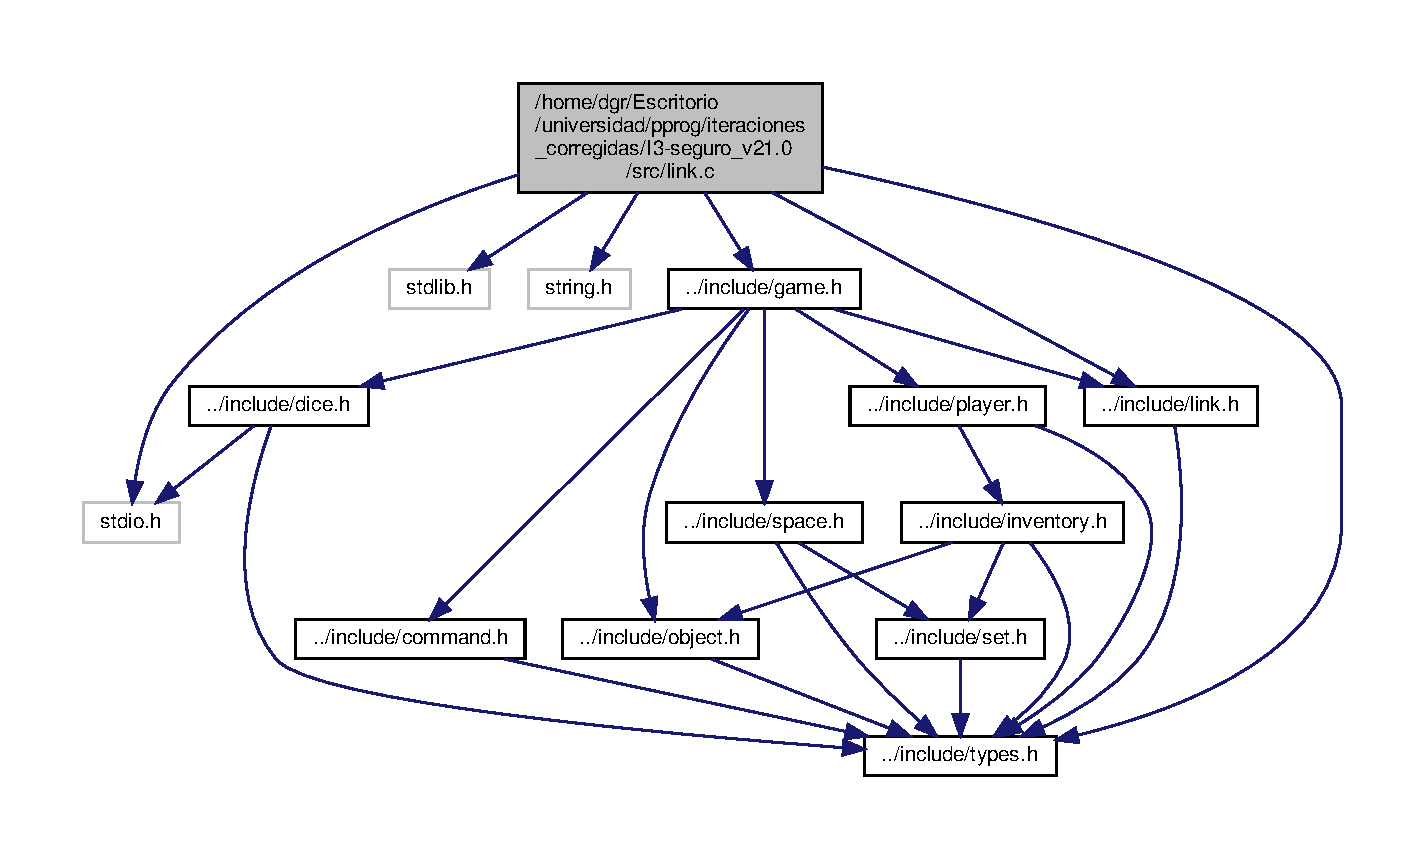
\includegraphics[width=350pt]{link_8c__incl}
\end{center}
\end{figure}
\subsection*{Data Structures}
\begin{DoxyCompactItemize}
\item 
struct \hyperlink{struct__Link}{\+\_\+\+Link}
\begin{DoxyCompactList}\small\item\em The link structure. \end{DoxyCompactList}\end{DoxyCompactItemize}
\subsection*{Functions}
\begin{DoxyCompactItemize}
\item 
\hyperlink{link_8h_ae3b299941e67be6971bfd64a25505eff}{Link} $\ast$ \hyperlink{link_8c_a8090d7f529cfd6a2fc5df3dd379fe514}{link\+\_\+create} (\hyperlink{types_8h_a845e604fb28f7e3d97549da3448149d3}{Id} id)
\begin{DoxyCompactList}\small\item\em Create the link, initialite the variables of the link. \end{DoxyCompactList}\item 
\hyperlink{types_8h_a32c27cc471df37f4fc818d65de0a56c4}{S\+T\+A\+T\+US} \hyperlink{link_8c_a6c7a3bd7a856288c377edbcd045912e6}{link\+\_\+set\+\_\+name} (\hyperlink{link_8h_ae3b299941e67be6971bfd64a25505eff}{Link} $\ast$link, char $\ast$name)
\begin{DoxyCompactList}\small\item\em set the name of a link \end{DoxyCompactList}\item 
\hyperlink{types_8h_a32c27cc471df37f4fc818d65de0a56c4}{S\+T\+A\+T\+US} \hyperlink{link_8c_a0f3653e949a03e7cac22d2503f8dc6f4}{link\+\_\+set\+\_\+id1} (\hyperlink{link_8h_ae3b299941e67be6971bfd64a25505eff}{Link} $\ast$link, \hyperlink{types_8h_a845e604fb28f7e3d97549da3448149d3}{Id} id)
\begin{DoxyCompactList}\small\item\em set the id1 of a link \end{DoxyCompactList}\item 
\hyperlink{types_8h_a32c27cc471df37f4fc818d65de0a56c4}{S\+T\+A\+T\+US} \hyperlink{link_8c_af3f534402173518ac4fb4880dad3f746}{link\+\_\+set\+\_\+id2} (\hyperlink{link_8h_ae3b299941e67be6971bfd64a25505eff}{Link} $\ast$link, \hyperlink{types_8h_a845e604fb28f7e3d97549da3448149d3}{Id} id)
\begin{DoxyCompactList}\small\item\em set the id2 of a link \end{DoxyCompactList}\item 
\hyperlink{types_8h_a32c27cc471df37f4fc818d65de0a56c4}{S\+T\+A\+T\+US} \hyperlink{link_8c_a7e7cd0c8f7c159bf689db53ee87e1bec}{link\+\_\+set\+\_\+open} (\hyperlink{link_8h_ae3b299941e67be6971bfd64a25505eff}{Link} $\ast$link, int open)
\begin{DoxyCompactList}\small\item\em set if the link is closed (1) or open (0) \end{DoxyCompactList}\item 
\hyperlink{types_8h_a32c27cc471df37f4fc818d65de0a56c4}{S\+T\+A\+T\+US} \hyperlink{link_8c_aff9d8ce68a82447a78449fda68f9e755}{link\+\_\+destory} (\hyperlink{link_8h_ae3b299941e67be6971bfd64a25505eff}{Link} $\ast$link)
\begin{DoxyCompactList}\small\item\em destroy a link \end{DoxyCompactList}\item 
\hyperlink{types_8h_a845e604fb28f7e3d97549da3448149d3}{Id} \hyperlink{link_8c_a2bbd320f995a72b2ea7ea639b1c81892}{link\+\_\+get\+\_\+id} (\hyperlink{link_8h_ae3b299941e67be6971bfd64a25505eff}{Link} $\ast$link)
\begin{DoxyCompactList}\small\item\em returns the id of the link that recive \end{DoxyCompactList}\item 
char $\ast$ \hyperlink{link_8c_a9747ee8201a323e112e67bdeacbc90d8}{link\+\_\+get\+\_\+name} (\hyperlink{link_8h_ae3b299941e67be6971bfd64a25505eff}{Link} $\ast$link)
\begin{DoxyCompactList}\small\item\em returns the name of the link that recive \end{DoxyCompactList}\item 
\hyperlink{types_8h_a845e604fb28f7e3d97549da3448149d3}{Id} \hyperlink{link_8c_ad39f5441c13abcb0fce07a81674b04ba}{link\+\_\+get\+\_\+id1} (\hyperlink{link_8h_ae3b299941e67be6971bfd64a25505eff}{Link} $\ast$link)
\begin{DoxyCompactList}\small\item\em returns the id1 of the link that recive \end{DoxyCompactList}\item 
\hyperlink{types_8h_a845e604fb28f7e3d97549da3448149d3}{Id} \hyperlink{link_8c_a2079fe643f883e3dcc3c47f9fde4852b}{link\+\_\+get\+\_\+id2} (\hyperlink{link_8h_ae3b299941e67be6971bfd64a25505eff}{Link} $\ast$link)
\begin{DoxyCompactList}\small\item\em returns the id2 of the link that recive \end{DoxyCompactList}\item 
\hyperlink{types_8h_a3e5b8192e7d9ffaf3542f1210aec18dd}{B\+O\+OL} \hyperlink{link_8c_a9fab05d77f8cd191a6675ccc6b9d585b}{link\+\_\+is\+\_\+open} (\hyperlink{link_8h_ae3b299941e67be6971bfd64a25505eff}{Link} $\ast$link)
\begin{DoxyCompactList}\small\item\em returns True in case that the link is open, False otherwise \end{DoxyCompactList}\item 
\hyperlink{types_8h_a32c27cc471df37f4fc818d65de0a56c4}{S\+T\+A\+T\+US} \hyperlink{link_8c_a7e0c894d83dbccbf58579b21fd565bb3}{link\+\_\+print} (F\+I\+LE $\ast$f, \hyperlink{link_8h_ae3b299941e67be6971bfd64a25505eff}{Link} $\ast$link)
\begin{DoxyCompactList}\small\item\em prints the information of a link \end{DoxyCompactList}\end{DoxyCompactItemize}


\subsection{Detailed Description}
It implements the link interface. 

\begin{DoxyAuthor}{Author}
David Teófilo Garitagoitia Romero 
\end{DoxyAuthor}
\begin{DoxyVersion}{Version}
1.\+0 
\end{DoxyVersion}
\begin{DoxyDate}{Date}
17-\/03-\/2020 
\end{DoxyDate}
\begin{DoxyCopyright}{Copyright}
G\+NU Public License 
\end{DoxyCopyright}


\subsection{Function Documentation}
\mbox{\Hypertarget{link_8c_a8090d7f529cfd6a2fc5df3dd379fe514}\label{link_8c_a8090d7f529cfd6a2fc5df3dd379fe514}} 
\index{link.\+c@{link.\+c}!link\+\_\+create@{link\+\_\+create}}
\index{link\+\_\+create@{link\+\_\+create}!link.\+c@{link.\+c}}
\subsubsection{\texorpdfstring{link\+\_\+create()}{link\_create()}}
{\footnotesize\ttfamily \hyperlink{link_8h_ae3b299941e67be6971bfd64a25505eff}{Link}$\ast$ link\+\_\+create (\begin{DoxyParamCaption}\item[{\hyperlink{types_8h_a845e604fb28f7e3d97549da3448149d3}{Id}}]{id }\end{DoxyParamCaption})}



Create the link, initialite the variables of the link. 

link\+\_\+create

\begin{DoxyDate}{Date}
17-\/03-\/2020 
\end{DoxyDate}
\begin{DoxyAuthor}{Author}
David Teófilo Garitagoitia Romero
\end{DoxyAuthor}

\begin{DoxyParams}{Parameters}
{\em id} & the id of the new link \\
\hline
\end{DoxyParams}
\begin{DoxyReturn}{Returns}
the link created 
\end{DoxyReturn}
\mbox{\Hypertarget{link_8c_aff9d8ce68a82447a78449fda68f9e755}\label{link_8c_aff9d8ce68a82447a78449fda68f9e755}} 
\index{link.\+c@{link.\+c}!link\+\_\+destory@{link\+\_\+destory}}
\index{link\+\_\+destory@{link\+\_\+destory}!link.\+c@{link.\+c}}
\subsubsection{\texorpdfstring{link\+\_\+destory()}{link\_destory()}}
{\footnotesize\ttfamily \hyperlink{types_8h_a32c27cc471df37f4fc818d65de0a56c4}{S\+T\+A\+T\+US} link\+\_\+destory (\begin{DoxyParamCaption}\item[{\hyperlink{link_8h_ae3b299941e67be6971bfd64a25505eff}{Link} $\ast$}]{link }\end{DoxyParamCaption})}



destroy a link 

link\+\_\+destroy

\begin{DoxyDate}{Date}
17-\/03-\/2020 
\end{DoxyDate}
\begin{DoxyAuthor}{Author}
David Teófilo Garitagoitia Romero
\end{DoxyAuthor}

\begin{DoxyParams}{Parameters}
{\em link} & the link we want to destroy \\
\hline
\end{DoxyParams}
\begin{DoxyReturn}{Returns}
Ok if there is no error, error otherwise 
\end{DoxyReturn}
\mbox{\Hypertarget{link_8c_a2bbd320f995a72b2ea7ea639b1c81892}\label{link_8c_a2bbd320f995a72b2ea7ea639b1c81892}} 
\index{link.\+c@{link.\+c}!link\+\_\+get\+\_\+id@{link\+\_\+get\+\_\+id}}
\index{link\+\_\+get\+\_\+id@{link\+\_\+get\+\_\+id}!link.\+c@{link.\+c}}
\subsubsection{\texorpdfstring{link\+\_\+get\+\_\+id()}{link\_get\_id()}}
{\footnotesize\ttfamily \hyperlink{types_8h_a845e604fb28f7e3d97549da3448149d3}{Id} link\+\_\+get\+\_\+id (\begin{DoxyParamCaption}\item[{\hyperlink{link_8h_ae3b299941e67be6971bfd64a25505eff}{Link} $\ast$}]{link }\end{DoxyParamCaption})}



returns the id of the link that recive 

link\+\_\+get\+\_\+id

\begin{DoxyDate}{Date}
17-\/03-\/2020 
\end{DoxyDate}
\begin{DoxyAuthor}{Author}
David Teófilo Garitagoitia Romero
\end{DoxyAuthor}

\begin{DoxyParams}{Parameters}
{\em link} & the link of which you want to know their id \\
\hline
\end{DoxyParams}
\begin{DoxyReturn}{Returns}
the id of the link that it recive 
\end{DoxyReturn}
\mbox{\Hypertarget{link_8c_ad39f5441c13abcb0fce07a81674b04ba}\label{link_8c_ad39f5441c13abcb0fce07a81674b04ba}} 
\index{link.\+c@{link.\+c}!link\+\_\+get\+\_\+id1@{link\+\_\+get\+\_\+id1}}
\index{link\+\_\+get\+\_\+id1@{link\+\_\+get\+\_\+id1}!link.\+c@{link.\+c}}
\subsubsection{\texorpdfstring{link\+\_\+get\+\_\+id1()}{link\_get\_id1()}}
{\footnotesize\ttfamily \hyperlink{types_8h_a845e604fb28f7e3d97549da3448149d3}{Id} link\+\_\+get\+\_\+id1 (\begin{DoxyParamCaption}\item[{\hyperlink{link_8h_ae3b299941e67be6971bfd64a25505eff}{Link} $\ast$}]{link }\end{DoxyParamCaption})}



returns the id1 of the link that recive 

link\+\_\+get\+\_\+id1

\begin{DoxyDate}{Date}
17-\/03-\/2020 
\end{DoxyDate}
\begin{DoxyAuthor}{Author}
David Teófilo Garitagoitia Romero
\end{DoxyAuthor}

\begin{DoxyParams}{Parameters}
{\em link} & the link of which you want to know their id1 \\
\hline
\end{DoxyParams}
\begin{DoxyReturn}{Returns}
the id1 of the link that it recives 
\end{DoxyReturn}
\mbox{\Hypertarget{link_8c_a2079fe643f883e3dcc3c47f9fde4852b}\label{link_8c_a2079fe643f883e3dcc3c47f9fde4852b}} 
\index{link.\+c@{link.\+c}!link\+\_\+get\+\_\+id2@{link\+\_\+get\+\_\+id2}}
\index{link\+\_\+get\+\_\+id2@{link\+\_\+get\+\_\+id2}!link.\+c@{link.\+c}}
\subsubsection{\texorpdfstring{link\+\_\+get\+\_\+id2()}{link\_get\_id2()}}
{\footnotesize\ttfamily \hyperlink{types_8h_a845e604fb28f7e3d97549da3448149d3}{Id} link\+\_\+get\+\_\+id2 (\begin{DoxyParamCaption}\item[{\hyperlink{link_8h_ae3b299941e67be6971bfd64a25505eff}{Link} $\ast$}]{link }\end{DoxyParamCaption})}



returns the id2 of the link that recive 

link\+\_\+get\+\_\+id2

\begin{DoxyDate}{Date}
17-\/03-\/2020 
\end{DoxyDate}
\begin{DoxyAuthor}{Author}
David Teófilo Garitagoitia Romero
\end{DoxyAuthor}

\begin{DoxyParams}{Parameters}
{\em link} & the link of which you want to know their id2 \\
\hline
\end{DoxyParams}
\begin{DoxyReturn}{Returns}
the id2 of the link that it recives 
\end{DoxyReturn}
\mbox{\Hypertarget{link_8c_a9747ee8201a323e112e67bdeacbc90d8}\label{link_8c_a9747ee8201a323e112e67bdeacbc90d8}} 
\index{link.\+c@{link.\+c}!link\+\_\+get\+\_\+name@{link\+\_\+get\+\_\+name}}
\index{link\+\_\+get\+\_\+name@{link\+\_\+get\+\_\+name}!link.\+c@{link.\+c}}
\subsubsection{\texorpdfstring{link\+\_\+get\+\_\+name()}{link\_get\_name()}}
{\footnotesize\ttfamily char$\ast$ link\+\_\+get\+\_\+name (\begin{DoxyParamCaption}\item[{\hyperlink{link_8h_ae3b299941e67be6971bfd64a25505eff}{Link} $\ast$}]{link }\end{DoxyParamCaption})}



returns the name of the link that recive 

link\+\_\+get\+\_\+name

\begin{DoxyDate}{Date}
17-\/03-\/2020 
\end{DoxyDate}
\begin{DoxyAuthor}{Author}
David Teófilo Garitagoitia Romero
\end{DoxyAuthor}

\begin{DoxyParams}{Parameters}
{\em link} & the link of which you want to know their name \\
\hline
\end{DoxyParams}
\begin{DoxyReturn}{Returns}
the name of the link that it recives 
\end{DoxyReturn}
\mbox{\Hypertarget{link_8c_a9fab05d77f8cd191a6675ccc6b9d585b}\label{link_8c_a9fab05d77f8cd191a6675ccc6b9d585b}} 
\index{link.\+c@{link.\+c}!link\+\_\+is\+\_\+open@{link\+\_\+is\+\_\+open}}
\index{link\+\_\+is\+\_\+open@{link\+\_\+is\+\_\+open}!link.\+c@{link.\+c}}
\subsubsection{\texorpdfstring{link\+\_\+is\+\_\+open()}{link\_is\_open()}}
{\footnotesize\ttfamily \hyperlink{types_8h_a3e5b8192e7d9ffaf3542f1210aec18dd}{B\+O\+OL} link\+\_\+is\+\_\+open (\begin{DoxyParamCaption}\item[{\hyperlink{link_8h_ae3b299941e67be6971bfd64a25505eff}{Link} $\ast$}]{link }\end{DoxyParamCaption})}



returns True in case that the link is open, False otherwise 

link\+\_\+is\+\_\+open

\begin{DoxyDate}{Date}
17-\/03-\/2020 
\end{DoxyDate}
\begin{DoxyAuthor}{Author}
David Teófilo Garitagoitia Romero
\end{DoxyAuthor}

\begin{DoxyParams}{Parameters}
{\em link} & the link of which you want to know if its open or not \\
\hline
\end{DoxyParams}
\begin{DoxyReturn}{Returns}
True in case that the link is open, False otherwise 
\end{DoxyReturn}
\mbox{\Hypertarget{link_8c_a7e0c894d83dbccbf58579b21fd565bb3}\label{link_8c_a7e0c894d83dbccbf58579b21fd565bb3}} 
\index{link.\+c@{link.\+c}!link\+\_\+print@{link\+\_\+print}}
\index{link\+\_\+print@{link\+\_\+print}!link.\+c@{link.\+c}}
\subsubsection{\texorpdfstring{link\+\_\+print()}{link\_print()}}
{\footnotesize\ttfamily \hyperlink{types_8h_a32c27cc471df37f4fc818d65de0a56c4}{S\+T\+A\+T\+US} link\+\_\+print (\begin{DoxyParamCaption}\item[{F\+I\+LE $\ast$}]{f,  }\item[{\hyperlink{link_8h_ae3b299941e67be6971bfd64a25505eff}{Link} $\ast$}]{link }\end{DoxyParamCaption})}



prints the information of a link 

link\+\_\+print

\begin{DoxyDate}{Date}
17-\/03-\/2020 
\end{DoxyDate}
\begin{DoxyAuthor}{Author}
David Teófilo Garitagoitia Romero
\end{DoxyAuthor}

\begin{DoxyParams}{Parameters}
{\em link} & the link we want to print \\
\hline
{\em f} & the file in which we want to print \\
\hline
\end{DoxyParams}
\begin{DoxyReturn}{Returns}
Ok if there is no error, error otherwise 
\end{DoxyReturn}
\mbox{\Hypertarget{link_8c_a0f3653e949a03e7cac22d2503f8dc6f4}\label{link_8c_a0f3653e949a03e7cac22d2503f8dc6f4}} 
\index{link.\+c@{link.\+c}!link\+\_\+set\+\_\+id1@{link\+\_\+set\+\_\+id1}}
\index{link\+\_\+set\+\_\+id1@{link\+\_\+set\+\_\+id1}!link.\+c@{link.\+c}}
\subsubsection{\texorpdfstring{link\+\_\+set\+\_\+id1()}{link\_set\_id1()}}
{\footnotesize\ttfamily \hyperlink{types_8h_a32c27cc471df37f4fc818d65de0a56c4}{S\+T\+A\+T\+US} link\+\_\+set\+\_\+id1 (\begin{DoxyParamCaption}\item[{\hyperlink{link_8h_ae3b299941e67be6971bfd64a25505eff}{Link} $\ast$}]{link,  }\item[{\hyperlink{types_8h_a845e604fb28f7e3d97549da3448149d3}{Id}}]{id }\end{DoxyParamCaption})}



set the id1 of a link 

link\+\_\+set\+\_\+id1

\begin{DoxyDate}{Date}
17-\/03-\/2020 
\end{DoxyDate}
\begin{DoxyAuthor}{Author}
David Teófilo Garitagoitia Romero
\end{DoxyAuthor}

\begin{DoxyParams}{Parameters}
{\em link} & the link in which we want to set the id1 \\
\hline
{\em id} & the id1 we want to set \\
\hline
\end{DoxyParams}
\begin{DoxyReturn}{Returns}
Ok if there is no error, error otherwise 
\end{DoxyReturn}
\mbox{\Hypertarget{link_8c_af3f534402173518ac4fb4880dad3f746}\label{link_8c_af3f534402173518ac4fb4880dad3f746}} 
\index{link.\+c@{link.\+c}!link\+\_\+set\+\_\+id2@{link\+\_\+set\+\_\+id2}}
\index{link\+\_\+set\+\_\+id2@{link\+\_\+set\+\_\+id2}!link.\+c@{link.\+c}}
\subsubsection{\texorpdfstring{link\+\_\+set\+\_\+id2()}{link\_set\_id2()}}
{\footnotesize\ttfamily \hyperlink{types_8h_a32c27cc471df37f4fc818d65de0a56c4}{S\+T\+A\+T\+US} link\+\_\+set\+\_\+id2 (\begin{DoxyParamCaption}\item[{\hyperlink{link_8h_ae3b299941e67be6971bfd64a25505eff}{Link} $\ast$}]{link,  }\item[{\hyperlink{types_8h_a845e604fb28f7e3d97549da3448149d3}{Id}}]{id }\end{DoxyParamCaption})}



set the id2 of a link 

link\+\_\+set\+\_\+id1

\begin{DoxyDate}{Date}
17-\/03-\/2020 
\end{DoxyDate}
\begin{DoxyAuthor}{Author}
David Teófilo Garitagoitia Romero
\end{DoxyAuthor}

\begin{DoxyParams}{Parameters}
{\em link} & the link in which we want to set the id2 \\
\hline
{\em id} & the id2 we want to set \\
\hline
\end{DoxyParams}
\begin{DoxyReturn}{Returns}
Ok if there is no error, error otherwise 
\end{DoxyReturn}
\mbox{\Hypertarget{link_8c_a6c7a3bd7a856288c377edbcd045912e6}\label{link_8c_a6c7a3bd7a856288c377edbcd045912e6}} 
\index{link.\+c@{link.\+c}!link\+\_\+set\+\_\+name@{link\+\_\+set\+\_\+name}}
\index{link\+\_\+set\+\_\+name@{link\+\_\+set\+\_\+name}!link.\+c@{link.\+c}}
\subsubsection{\texorpdfstring{link\+\_\+set\+\_\+name()}{link\_set\_name()}}
{\footnotesize\ttfamily \hyperlink{types_8h_a32c27cc471df37f4fc818d65de0a56c4}{S\+T\+A\+T\+US} link\+\_\+set\+\_\+name (\begin{DoxyParamCaption}\item[{\hyperlink{link_8h_ae3b299941e67be6971bfd64a25505eff}{Link} $\ast$}]{link,  }\item[{char $\ast$}]{name }\end{DoxyParamCaption})}



set the name of a link 

link\+\_\+set\+\_\+name

\begin{DoxyDate}{Date}
17-\/03-\/2020 
\end{DoxyDate}
\begin{DoxyAuthor}{Author}
David Teófilo Garitagoitia Romero
\end{DoxyAuthor}

\begin{DoxyParams}{Parameters}
{\em link} & the link in which we want to set the name \\
\hline
{\em name} & the name we want to set \\
\hline
\end{DoxyParams}
\begin{DoxyReturn}{Returns}
Ok if there is no error, error otherwise 
\end{DoxyReturn}
\mbox{\Hypertarget{link_8c_a7e7cd0c8f7c159bf689db53ee87e1bec}\label{link_8c_a7e7cd0c8f7c159bf689db53ee87e1bec}} 
\index{link.\+c@{link.\+c}!link\+\_\+set\+\_\+open@{link\+\_\+set\+\_\+open}}
\index{link\+\_\+set\+\_\+open@{link\+\_\+set\+\_\+open}!link.\+c@{link.\+c}}
\subsubsection{\texorpdfstring{link\+\_\+set\+\_\+open()}{link\_set\_open()}}
{\footnotesize\ttfamily \hyperlink{types_8h_a32c27cc471df37f4fc818d65de0a56c4}{S\+T\+A\+T\+US} link\+\_\+set\+\_\+open (\begin{DoxyParamCaption}\item[{\hyperlink{link_8h_ae3b299941e67be6971bfd64a25505eff}{Link} $\ast$}]{link,  }\item[{int}]{open }\end{DoxyParamCaption})}



set if the link is closed (1) or open (0) 

link\+\_\+set\+\_\+open

\begin{DoxyDate}{Date}
17-\/03-\/2020 
\end{DoxyDate}
\begin{DoxyAuthor}{Author}
David Teófilo Garitagoitia Romero
\end{DoxyAuthor}

\begin{DoxyParams}{Parameters}
{\em link} & the link in which we want to set the id1 \\
\hline
{\em open} & if the link is open (0), otherwise 1 \\
\hline
\end{DoxyParams}
\begin{DoxyReturn}{Returns}
Ok if there is no error, error otherwise 
\end{DoxyReturn}

\hypertarget{link__test_8c}{}\section{src/link\+\_\+test.c File Reference}
\label{link__test_8c}\index{src/link\+\_\+test.\+c@{src/link\+\_\+test.\+c}}


test to see if links works correctly  


{\ttfamily \#include $<$stdio.\+h$>$}\newline
{\ttfamily \#include $<$string.\+h$>$}\newline
{\ttfamily \#include $<$stdlib.\+h$>$}\newline
{\ttfamily \#include \char`\"{}../include/link.\+h\char`\"{}}\newline
{\ttfamily \#include \char`\"{}../include/test.\+h\char`\"{}}\newline
{\ttfamily \#include \char`\"{}../include/link\+\_\+test.\+h\char`\"{}}\newline
Include dependency graph for link\+\_\+test.\+c\+:\nopagebreak
\begin{figure}[H]
\begin{center}
\leavevmode
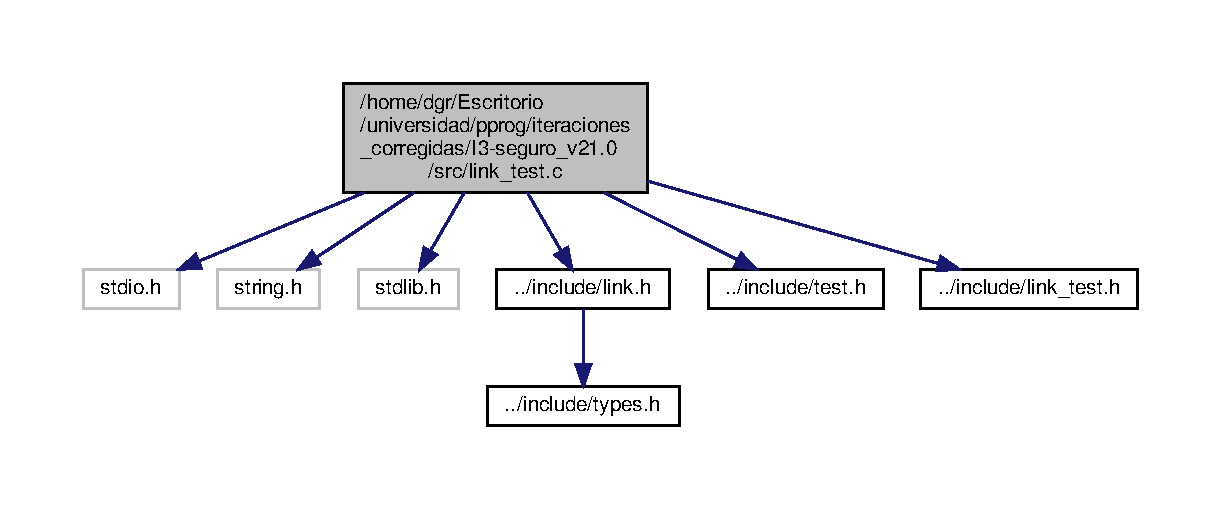
\includegraphics[width=350pt]{link__test_8c__incl}
\end{center}
\end{figure}
\subsection*{Macros}
\begin{DoxyCompactItemize}
\item 
\#define \hyperlink{link__test_8c_a2a77d2f2c5b698c69c19e1f8782bf709}{M\+A\+X\+\_\+\+T\+E\+S\+TS}~22
\begin{DoxyCompactList}\small\item\em maximum number of test \end{DoxyCompactList}\end{DoxyCompactItemize}
\subsection*{Functions}
\begin{DoxyCompactItemize}
\item 
int \hyperlink{link__test_8c_a3c04138a5bfe5d72780bb7e82a18e627}{main} (int argc, char $\ast$$\ast$argv)
\begin{DoxyCompactList}\small\item\em the main function of link\+\_\+test main \end{DoxyCompactList}\item 
void \hyperlink{link__test_8c_a82c5ee441ad22caad8272212a9e9cc26}{test1\+\_\+link\+\_\+create} ()
\item 
void \hyperlink{link__test_8c_a24b5463da176c3e578b0a0fa8bb1f9f0}{test2\+\_\+link\+\_\+create} ()
\item 
void \hyperlink{link__test_8c_ae0e478a0540bed26befc071591e3ff6c}{test1\+\_\+link\+\_\+set\+\_\+name} ()
\item 
void \hyperlink{link__test_8c_aa66c1e991620a5a758ba6e4d6b4a8b73}{test2\+\_\+link\+\_\+set\+\_\+name} ()
\item 
void \hyperlink{link__test_8c_a42d2fdbe0afa812eb94b9332ab8c3b79}{test1\+\_\+link\+\_\+set\+\_\+id1} ()
\item 
void \hyperlink{link__test_8c_acc401625c94cf6dc9ab66aa974804397}{test2\+\_\+link\+\_\+set\+\_\+id1} ()
\item 
void \hyperlink{link__test_8c_aa4ea6550c6521090364bb423a97724d3}{test1\+\_\+link\+\_\+set\+\_\+id2} ()
\item 
void \hyperlink{link__test_8c_a3a6a81c8b408b2e438884cb3e4d533a3}{test2\+\_\+link\+\_\+set\+\_\+id2} ()
\item 
void \hyperlink{link__test_8c_acbe99eb2aa596b7466ba69d1b78c3f3b}{test1\+\_\+link\+\_\+set\+\_\+open} ()
\item 
void \hyperlink{link__test_8c_a4f7f80db70fdda86df30c5e35c851d65}{test2\+\_\+link\+\_\+set\+\_\+open} ()
\item 
void \hyperlink{link__test_8c_ad4391bca80133c2afaa73a0e520b546e}{test3\+\_\+link\+\_\+set\+\_\+open} ()
\item 
void \hyperlink{link__test_8c_a19c70f79fd51d123173f7aaf6ae50bf8}{test1\+\_\+link\+\_\+get\+\_\+id} ()
\item 
void \hyperlink{link__test_8c_a0f967a1782dd7264e73ad428d22d125d}{test2\+\_\+link\+\_\+get\+\_\+id} ()
\item 
void \hyperlink{link__test_8c_ac3124af4c90d4769cd6e42849817528c}{test1\+\_\+link\+\_\+is\+\_\+open} ()
\item 
void \hyperlink{link__test_8c_a52754541d1357c38da41b0c1b120d5ed}{test2\+\_\+link\+\_\+is\+\_\+open} ()
\item 
void \hyperlink{link__test_8c_a316b5e1d082f5f7133529044b70caaaa}{test3\+\_\+link\+\_\+is\+\_\+open} ()
\item 
void \hyperlink{link__test_8c_ac45f246d7f9b1d21535c743bbb970a85}{test1\+\_\+link\+\_\+get\+\_\+id1} ()
\item 
void \hyperlink{link__test_8c_a26e61cc0a08c97282384a56212168d5a}{test2\+\_\+link\+\_\+get\+\_\+id1} ()
\item 
void \hyperlink{link__test_8c_aeaa87091cae85a91de5db2c755d4eee9}{test1\+\_\+link\+\_\+get\+\_\+id2} ()
\item 
void \hyperlink{link__test_8c_ad9c803361f84a47b5e3f0d475eeb28d0}{test2\+\_\+link\+\_\+get\+\_\+id2} ()
\item 
void \hyperlink{link__test_8c_a044128db00a5cc385d7157dea8bdf3c3}{test1\+\_\+link\+\_\+get\+\_\+name} ()
\item 
void \hyperlink{link__test_8c_a4efc6cfcdc210e2803f9d285734c571e}{test2\+\_\+link\+\_\+get\+\_\+name} ()
\end{DoxyCompactItemize}


\subsection{Detailed Description}
test to see if links works correctly 

\begin{DoxyAuthor}{Author}
Daniel Cerrato Sánchez 
\end{DoxyAuthor}
\begin{DoxyVersion}{Version}
2.\+0 
\end{DoxyVersion}
\begin{DoxyDate}{Date}
10-\/06-\/2020 
\end{DoxyDate}
\begin{DoxyCopyright}{Copyright}
G\+NU Public License 
\end{DoxyCopyright}


\subsection{Macro Definition Documentation}
\mbox{\Hypertarget{link__test_8c_a2a77d2f2c5b698c69c19e1f8782bf709}\label{link__test_8c_a2a77d2f2c5b698c69c19e1f8782bf709}} 
\index{link\+\_\+test.\+c@{link\+\_\+test.\+c}!M\+A\+X\+\_\+\+T\+E\+S\+TS@{M\+A\+X\+\_\+\+T\+E\+S\+TS}}
\index{M\+A\+X\+\_\+\+T\+E\+S\+TS@{M\+A\+X\+\_\+\+T\+E\+S\+TS}!link\+\_\+test.\+c@{link\+\_\+test.\+c}}
\subsubsection{\texorpdfstring{M\+A\+X\+\_\+\+T\+E\+S\+TS}{MAX\_TESTS}}
{\footnotesize\ttfamily \#define M\+A\+X\+\_\+\+T\+E\+S\+TS~22}



maximum number of test 

Details. 

\subsection{Function Documentation}
\mbox{\Hypertarget{link__test_8c_a3c04138a5bfe5d72780bb7e82a18e627}\label{link__test_8c_a3c04138a5bfe5d72780bb7e82a18e627}} 
\index{link\+\_\+test.\+c@{link\+\_\+test.\+c}!main@{main}}
\index{main@{main}!link\+\_\+test.\+c@{link\+\_\+test.\+c}}
\subsubsection{\texorpdfstring{main()}{main()}}
{\footnotesize\ttfamily int main (\begin{DoxyParamCaption}\item[{int}]{argc,  }\item[{char $\ast$$\ast$}]{argv }\end{DoxyParamCaption})}



the main function of link\+\_\+test main 

\begin{DoxyDate}{Date}
10-\/06-\/2020 
\end{DoxyDate}
\begin{DoxyAuthor}{Author}
Daniel Cerrato Sánchez 
\end{DoxyAuthor}
\begin{DoxyReturn}{Returns}

\end{DoxyReturn}
\mbox{\Hypertarget{link__test_8c_a82c5ee441ad22caad8272212a9e9cc26}\label{link__test_8c_a82c5ee441ad22caad8272212a9e9cc26}} 
\index{link\+\_\+test.\+c@{link\+\_\+test.\+c}!test1\+\_\+link\+\_\+create@{test1\+\_\+link\+\_\+create}}
\index{test1\+\_\+link\+\_\+create@{test1\+\_\+link\+\_\+create}!link\+\_\+test.\+c@{link\+\_\+test.\+c}}
\subsubsection{\texorpdfstring{test1\+\_\+link\+\_\+create()}{test1\_link\_create()}}
{\footnotesize\ttfamily void test1\+\_\+link\+\_\+create (\begin{DoxyParamCaption}{ }\end{DoxyParamCaption})}

\begin{DoxyRefDesc}{Test}
\item[\hyperlink{test__test000112}{Test}]Test the link creation function \end{DoxyRefDesc}
\begin{DoxyPrecond}{Precondition}
An id as parameter 
\end{DoxyPrecond}
\begin{DoxyPostcond}{Postcondition}
A non-\/null pointer to the created link 
\end{DoxyPostcond}
\mbox{\Hypertarget{link__test_8c_a19c70f79fd51d123173f7aaf6ae50bf8}\label{link__test_8c_a19c70f79fd51d123173f7aaf6ae50bf8}} 
\index{link\+\_\+test.\+c@{link\+\_\+test.\+c}!test1\+\_\+link\+\_\+get\+\_\+id@{test1\+\_\+link\+\_\+get\+\_\+id}}
\index{test1\+\_\+link\+\_\+get\+\_\+id@{test1\+\_\+link\+\_\+get\+\_\+id}!link\+\_\+test.\+c@{link\+\_\+test.\+c}}
\subsubsection{\texorpdfstring{test1\+\_\+link\+\_\+get\+\_\+id()}{test1\_link\_get\_id()}}
{\footnotesize\ttfamily void test1\+\_\+link\+\_\+get\+\_\+id (\begin{DoxyParamCaption}{ }\end{DoxyParamCaption})}

\begin{DoxyRefDesc}{Test}
\item[\hyperlink{test__test000123}{Test}]Test the function to get the id of a link \end{DoxyRefDesc}
\begin{DoxyPrecond}{Precondition}
The link is a non-\/\+N\+U\+LL pointer with correct id 
\end{DoxyPrecond}
\begin{DoxyPostcond}{Postcondition}
The output must be the id entered when creating it 
\end{DoxyPostcond}
\mbox{\Hypertarget{link__test_8c_ac45f246d7f9b1d21535c743bbb970a85}\label{link__test_8c_ac45f246d7f9b1d21535c743bbb970a85}} 
\index{link\+\_\+test.\+c@{link\+\_\+test.\+c}!test1\+\_\+link\+\_\+get\+\_\+id1@{test1\+\_\+link\+\_\+get\+\_\+id1}}
\index{test1\+\_\+link\+\_\+get\+\_\+id1@{test1\+\_\+link\+\_\+get\+\_\+id1}!link\+\_\+test.\+c@{link\+\_\+test.\+c}}
\subsubsection{\texorpdfstring{test1\+\_\+link\+\_\+get\+\_\+id1()}{test1\_link\_get\_id1()}}
{\footnotesize\ttfamily void test1\+\_\+link\+\_\+get\+\_\+id1 (\begin{DoxyParamCaption}{ }\end{DoxyParamCaption})}

\begin{DoxyRefDesc}{Test}
\item[\hyperlink{test__test000128}{Test}]Test the function to get the exit id of a link \end{DoxyRefDesc}
\begin{DoxyPrecond}{Precondition}
The link is a non-\/\+N\+U\+LL pointer with correct exit id 
\end{DoxyPrecond}
\begin{DoxyPostcond}{Postcondition}
The output must be the output id 
\end{DoxyPostcond}
\mbox{\Hypertarget{link__test_8c_aeaa87091cae85a91de5db2c755d4eee9}\label{link__test_8c_aeaa87091cae85a91de5db2c755d4eee9}} 
\index{link\+\_\+test.\+c@{link\+\_\+test.\+c}!test1\+\_\+link\+\_\+get\+\_\+id2@{test1\+\_\+link\+\_\+get\+\_\+id2}}
\index{test1\+\_\+link\+\_\+get\+\_\+id2@{test1\+\_\+link\+\_\+get\+\_\+id2}!link\+\_\+test.\+c@{link\+\_\+test.\+c}}
\subsubsection{\texorpdfstring{test1\+\_\+link\+\_\+get\+\_\+id2()}{test1\_link\_get\_id2()}}
{\footnotesize\ttfamily void test1\+\_\+link\+\_\+get\+\_\+id2 (\begin{DoxyParamCaption}{ }\end{DoxyParamCaption})}

\begin{DoxyRefDesc}{Test}
\item[\hyperlink{test__test000130}{Test}]Test the function to get the input id of a link \end{DoxyRefDesc}
\begin{DoxyPrecond}{Precondition}
The link is a non-\/\+N\+U\+LL pointer with correct input id 
\end{DoxyPrecond}
\begin{DoxyPostcond}{Postcondition}
The output must be the input id 
\end{DoxyPostcond}
\mbox{\Hypertarget{link__test_8c_a044128db00a5cc385d7157dea8bdf3c3}\label{link__test_8c_a044128db00a5cc385d7157dea8bdf3c3}} 
\index{link\+\_\+test.\+c@{link\+\_\+test.\+c}!test1\+\_\+link\+\_\+get\+\_\+name@{test1\+\_\+link\+\_\+get\+\_\+name}}
\index{test1\+\_\+link\+\_\+get\+\_\+name@{test1\+\_\+link\+\_\+get\+\_\+name}!link\+\_\+test.\+c@{link\+\_\+test.\+c}}
\subsubsection{\texorpdfstring{test1\+\_\+link\+\_\+get\+\_\+name()}{test1\_link\_get\_name()}}
{\footnotesize\ttfamily void test1\+\_\+link\+\_\+get\+\_\+name (\begin{DoxyParamCaption}{ }\end{DoxyParamCaption})}

\begin{DoxyRefDesc}{Test}
\item[\hyperlink{test__test000132}{Test}]Test the function to get the name of a link \end{DoxyRefDesc}
\begin{DoxyPrecond}{Precondition}
The link is a non-\/\+N\+U\+LL pointer with correct name 
\end{DoxyPrecond}
\begin{DoxyPostcond}{Postcondition}
The comparison between the name and the word to compare must be 0 
\end{DoxyPostcond}
\mbox{\Hypertarget{link__test_8c_ac3124af4c90d4769cd6e42849817528c}\label{link__test_8c_ac3124af4c90d4769cd6e42849817528c}} 
\index{link\+\_\+test.\+c@{link\+\_\+test.\+c}!test1\+\_\+link\+\_\+is\+\_\+open@{test1\+\_\+link\+\_\+is\+\_\+open}}
\index{test1\+\_\+link\+\_\+is\+\_\+open@{test1\+\_\+link\+\_\+is\+\_\+open}!link\+\_\+test.\+c@{link\+\_\+test.\+c}}
\subsubsection{\texorpdfstring{test1\+\_\+link\+\_\+is\+\_\+open()}{test1\_link\_is\_open()}}
{\footnotesize\ttfamily void test1\+\_\+link\+\_\+is\+\_\+open (\begin{DoxyParamCaption}{ }\end{DoxyParamCaption})}

\begin{DoxyRefDesc}{Test}
\item[\hyperlink{test__test000125}{Test}]Test the function to get the opening status of a link \end{DoxyRefDesc}
\begin{DoxyPrecond}{Precondition}
The link is a non-\/\+N\+U\+LL pointer with status 0 (open) 
\end{DoxyPrecond}
\begin{DoxyPostcond}{Postcondition}
The output must be T\+R\+UE 
\end{DoxyPostcond}
\mbox{\Hypertarget{link__test_8c_a42d2fdbe0afa812eb94b9332ab8c3b79}\label{link__test_8c_a42d2fdbe0afa812eb94b9332ab8c3b79}} 
\index{link\+\_\+test.\+c@{link\+\_\+test.\+c}!test1\+\_\+link\+\_\+set\+\_\+id1@{test1\+\_\+link\+\_\+set\+\_\+id1}}
\index{test1\+\_\+link\+\_\+set\+\_\+id1@{test1\+\_\+link\+\_\+set\+\_\+id1}!link\+\_\+test.\+c@{link\+\_\+test.\+c}}
\subsubsection{\texorpdfstring{test1\+\_\+link\+\_\+set\+\_\+id1()}{test1\_link\_set\_id1()}}
{\footnotesize\ttfamily void test1\+\_\+link\+\_\+set\+\_\+id1 (\begin{DoxyParamCaption}{ }\end{DoxyParamCaption})}

\begin{DoxyRefDesc}{Test}
\item[\hyperlink{test__test000116}{Test}]Test the function to change the exit id of a link \end{DoxyRefDesc}
\begin{DoxyPrecond}{Precondition}
The link is a non-\/\+N\+U\+LL pointer, the exit id is correct 
\end{DoxyPrecond}
\begin{DoxyPostcond}{Postcondition}
The output must be OK 
\end{DoxyPostcond}
\mbox{\Hypertarget{link__test_8c_aa4ea6550c6521090364bb423a97724d3}\label{link__test_8c_aa4ea6550c6521090364bb423a97724d3}} 
\index{link\+\_\+test.\+c@{link\+\_\+test.\+c}!test1\+\_\+link\+\_\+set\+\_\+id2@{test1\+\_\+link\+\_\+set\+\_\+id2}}
\index{test1\+\_\+link\+\_\+set\+\_\+id2@{test1\+\_\+link\+\_\+set\+\_\+id2}!link\+\_\+test.\+c@{link\+\_\+test.\+c}}
\subsubsection{\texorpdfstring{test1\+\_\+link\+\_\+set\+\_\+id2()}{test1\_link\_set\_id2()}}
{\footnotesize\ttfamily void test1\+\_\+link\+\_\+set\+\_\+id2 (\begin{DoxyParamCaption}{ }\end{DoxyParamCaption})}

\begin{DoxyRefDesc}{Test}
\item[\hyperlink{test__test000118}{Test}]Test the function to change the input id of a link \end{DoxyRefDesc}
\begin{DoxyPrecond}{Precondition}
The link is a non-\/\+N\+U\+LL pointer, the input id is correct 
\end{DoxyPrecond}
\begin{DoxyPostcond}{Postcondition}
The output must be OK 
\end{DoxyPostcond}
\mbox{\Hypertarget{link__test_8c_ae0e478a0540bed26befc071591e3ff6c}\label{link__test_8c_ae0e478a0540bed26befc071591e3ff6c}} 
\index{link\+\_\+test.\+c@{link\+\_\+test.\+c}!test1\+\_\+link\+\_\+set\+\_\+name@{test1\+\_\+link\+\_\+set\+\_\+name}}
\index{test1\+\_\+link\+\_\+set\+\_\+name@{test1\+\_\+link\+\_\+set\+\_\+name}!link\+\_\+test.\+c@{link\+\_\+test.\+c}}
\subsubsection{\texorpdfstring{test1\+\_\+link\+\_\+set\+\_\+name()}{test1\_link\_set\_name()}}
{\footnotesize\ttfamily void test1\+\_\+link\+\_\+set\+\_\+name (\begin{DoxyParamCaption}{ }\end{DoxyParamCaption})}

\begin{DoxyRefDesc}{Test}
\item[\hyperlink{test__test000114}{Test}]Test the function to rename a link \end{DoxyRefDesc}
\begin{DoxyPrecond}{Precondition}
The link is a non-\/\+N\+U\+LL pointer, the name is correct 
\end{DoxyPrecond}
\begin{DoxyPostcond}{Postcondition}
The output must be OK 
\end{DoxyPostcond}
\mbox{\Hypertarget{link__test_8c_acbe99eb2aa596b7466ba69d1b78c3f3b}\label{link__test_8c_acbe99eb2aa596b7466ba69d1b78c3f3b}} 
\index{link\+\_\+test.\+c@{link\+\_\+test.\+c}!test1\+\_\+link\+\_\+set\+\_\+open@{test1\+\_\+link\+\_\+set\+\_\+open}}
\index{test1\+\_\+link\+\_\+set\+\_\+open@{test1\+\_\+link\+\_\+set\+\_\+open}!link\+\_\+test.\+c@{link\+\_\+test.\+c}}
\subsubsection{\texorpdfstring{test1\+\_\+link\+\_\+set\+\_\+open()}{test1\_link\_set\_open()}}
{\footnotesize\ttfamily void test1\+\_\+link\+\_\+set\+\_\+open (\begin{DoxyParamCaption}{ }\end{DoxyParamCaption})}

\begin{DoxyRefDesc}{Test}
\item[\hyperlink{test__test000120}{Test}]Test the function to change the opening state of a link \end{DoxyRefDesc}
\begin{DoxyPrecond}{Precondition}
The link is a non-\/\+N\+U\+LL pointer, the state is 0 (open) 
\end{DoxyPrecond}
\begin{DoxyPostcond}{Postcondition}
The output must be OK 
\end{DoxyPostcond}
\mbox{\Hypertarget{link__test_8c_a24b5463da176c3e578b0a0fa8bb1f9f0}\label{link__test_8c_a24b5463da176c3e578b0a0fa8bb1f9f0}} 
\index{link\+\_\+test.\+c@{link\+\_\+test.\+c}!test2\+\_\+link\+\_\+create@{test2\+\_\+link\+\_\+create}}
\index{test2\+\_\+link\+\_\+create@{test2\+\_\+link\+\_\+create}!link\+\_\+test.\+c@{link\+\_\+test.\+c}}
\subsubsection{\texorpdfstring{test2\+\_\+link\+\_\+create()}{test2\_link\_create()}}
{\footnotesize\ttfamily void test2\+\_\+link\+\_\+create (\begin{DoxyParamCaption}{ }\end{DoxyParamCaption})}

\begin{DoxyRefDesc}{Test}
\item[\hyperlink{test__test000113}{Test}]Test the link creation function \end{DoxyRefDesc}
\begin{DoxyPrecond}{Precondition}
The link is a non-\/\+N\+U\+LL pointer with correct id 
\end{DoxyPrecond}
\begin{DoxyPostcond}{Postcondition}
The link id must be the one entered when creating it 
\end{DoxyPostcond}
\mbox{\Hypertarget{link__test_8c_a0f967a1782dd7264e73ad428d22d125d}\label{link__test_8c_a0f967a1782dd7264e73ad428d22d125d}} 
\index{link\+\_\+test.\+c@{link\+\_\+test.\+c}!test2\+\_\+link\+\_\+get\+\_\+id@{test2\+\_\+link\+\_\+get\+\_\+id}}
\index{test2\+\_\+link\+\_\+get\+\_\+id@{test2\+\_\+link\+\_\+get\+\_\+id}!link\+\_\+test.\+c@{link\+\_\+test.\+c}}
\subsubsection{\texorpdfstring{test2\+\_\+link\+\_\+get\+\_\+id()}{test2\_link\_get\_id()}}
{\footnotesize\ttfamily void test2\+\_\+link\+\_\+get\+\_\+id (\begin{DoxyParamCaption}{ }\end{DoxyParamCaption})}

\begin{DoxyRefDesc}{Test}
\item[\hyperlink{test__test000124}{Test}]Test the function to get the id of a link \end{DoxyRefDesc}
\begin{DoxyPrecond}{Precondition}
The link is a pointer to N\+U\+LL 
\end{DoxyPrecond}
\begin{DoxyPostcond}{Postcondition}
The output must be N\+O\+\_\+\+ID 
\end{DoxyPostcond}
\mbox{\Hypertarget{link__test_8c_a26e61cc0a08c97282384a56212168d5a}\label{link__test_8c_a26e61cc0a08c97282384a56212168d5a}} 
\index{link\+\_\+test.\+c@{link\+\_\+test.\+c}!test2\+\_\+link\+\_\+get\+\_\+id1@{test2\+\_\+link\+\_\+get\+\_\+id1}}
\index{test2\+\_\+link\+\_\+get\+\_\+id1@{test2\+\_\+link\+\_\+get\+\_\+id1}!link\+\_\+test.\+c@{link\+\_\+test.\+c}}
\subsubsection{\texorpdfstring{test2\+\_\+link\+\_\+get\+\_\+id1()}{test2\_link\_get\_id1()}}
{\footnotesize\ttfamily void test2\+\_\+link\+\_\+get\+\_\+id1 (\begin{DoxyParamCaption}{ }\end{DoxyParamCaption})}

\begin{DoxyRefDesc}{Test}
\item[\hyperlink{test__test000129}{Test}]Test the function to get the exit id of a link \end{DoxyRefDesc}
\begin{DoxyPrecond}{Precondition}
The link is a pointer to N\+U\+LL 
\end{DoxyPrecond}
\begin{DoxyPostcond}{Postcondition}
The output must be N\+O\+\_\+\+ID 
\end{DoxyPostcond}
\mbox{\Hypertarget{link__test_8c_ad9c803361f84a47b5e3f0d475eeb28d0}\label{link__test_8c_ad9c803361f84a47b5e3f0d475eeb28d0}} 
\index{link\+\_\+test.\+c@{link\+\_\+test.\+c}!test2\+\_\+link\+\_\+get\+\_\+id2@{test2\+\_\+link\+\_\+get\+\_\+id2}}
\index{test2\+\_\+link\+\_\+get\+\_\+id2@{test2\+\_\+link\+\_\+get\+\_\+id2}!link\+\_\+test.\+c@{link\+\_\+test.\+c}}
\subsubsection{\texorpdfstring{test2\+\_\+link\+\_\+get\+\_\+id2()}{test2\_link\_get\_id2()}}
{\footnotesize\ttfamily void test2\+\_\+link\+\_\+get\+\_\+id2 (\begin{DoxyParamCaption}{ }\end{DoxyParamCaption})}

\begin{DoxyRefDesc}{Test}
\item[\hyperlink{test__test000131}{Test}]Test the function to get the input id of a link \end{DoxyRefDesc}
\begin{DoxyPrecond}{Precondition}
The link is a pointer to N\+U\+LL 
\end{DoxyPrecond}
\begin{DoxyPostcond}{Postcondition}
The output must be N\+O\+\_\+\+ID 
\end{DoxyPostcond}
\mbox{\Hypertarget{link__test_8c_a4efc6cfcdc210e2803f9d285734c571e}\label{link__test_8c_a4efc6cfcdc210e2803f9d285734c571e}} 
\index{link\+\_\+test.\+c@{link\+\_\+test.\+c}!test2\+\_\+link\+\_\+get\+\_\+name@{test2\+\_\+link\+\_\+get\+\_\+name}}
\index{test2\+\_\+link\+\_\+get\+\_\+name@{test2\+\_\+link\+\_\+get\+\_\+name}!link\+\_\+test.\+c@{link\+\_\+test.\+c}}
\subsubsection{\texorpdfstring{test2\+\_\+link\+\_\+get\+\_\+name()}{test2\_link\_get\_name()}}
{\footnotesize\ttfamily void test2\+\_\+link\+\_\+get\+\_\+name (\begin{DoxyParamCaption}{ }\end{DoxyParamCaption})}

\begin{DoxyRefDesc}{Test}
\item[\hyperlink{test__test000133}{Test}]Test the function to get the name of a link \end{DoxyRefDesc}
\begin{DoxyPrecond}{Precondition}
The link is a pointer to N\+U\+LL 
\end{DoxyPrecond}
\begin{DoxyPostcond}{Postcondition}
The output must be N\+U\+LL 
\end{DoxyPostcond}
\mbox{\Hypertarget{link__test_8c_a52754541d1357c38da41b0c1b120d5ed}\label{link__test_8c_a52754541d1357c38da41b0c1b120d5ed}} 
\index{link\+\_\+test.\+c@{link\+\_\+test.\+c}!test2\+\_\+link\+\_\+is\+\_\+open@{test2\+\_\+link\+\_\+is\+\_\+open}}
\index{test2\+\_\+link\+\_\+is\+\_\+open@{test2\+\_\+link\+\_\+is\+\_\+open}!link\+\_\+test.\+c@{link\+\_\+test.\+c}}
\subsubsection{\texorpdfstring{test2\+\_\+link\+\_\+is\+\_\+open()}{test2\_link\_is\_open()}}
{\footnotesize\ttfamily void test2\+\_\+link\+\_\+is\+\_\+open (\begin{DoxyParamCaption}{ }\end{DoxyParamCaption})}

\begin{DoxyRefDesc}{Test}
\item[\hyperlink{test__test000126}{Test}]Test the function to get the opening status of a link \end{DoxyRefDesc}
\begin{DoxyPrecond}{Precondition}
The link is a non-\/\+N\+U\+LL pointer with status 1 (closed) 
\end{DoxyPrecond}
\begin{DoxyPostcond}{Postcondition}
The output must be F\+A\+L\+SE 
\end{DoxyPostcond}
\mbox{\Hypertarget{link__test_8c_acc401625c94cf6dc9ab66aa974804397}\label{link__test_8c_acc401625c94cf6dc9ab66aa974804397}} 
\index{link\+\_\+test.\+c@{link\+\_\+test.\+c}!test2\+\_\+link\+\_\+set\+\_\+id1@{test2\+\_\+link\+\_\+set\+\_\+id1}}
\index{test2\+\_\+link\+\_\+set\+\_\+id1@{test2\+\_\+link\+\_\+set\+\_\+id1}!link\+\_\+test.\+c@{link\+\_\+test.\+c}}
\subsubsection{\texorpdfstring{test2\+\_\+link\+\_\+set\+\_\+id1()}{test2\_link\_set\_id1()}}
{\footnotesize\ttfamily void test2\+\_\+link\+\_\+set\+\_\+id1 (\begin{DoxyParamCaption}{ }\end{DoxyParamCaption})}

\begin{DoxyRefDesc}{Test}
\item[\hyperlink{test__test000117}{Test}]Test the function to change the exit id of a link \end{DoxyRefDesc}
\begin{DoxyPrecond}{Precondition}
The link is a pointer to N\+U\+LL 
\end{DoxyPrecond}
\begin{DoxyPostcond}{Postcondition}
The output must be E\+R\+R\+OR 
\end{DoxyPostcond}
\mbox{\Hypertarget{link__test_8c_a3a6a81c8b408b2e438884cb3e4d533a3}\label{link__test_8c_a3a6a81c8b408b2e438884cb3e4d533a3}} 
\index{link\+\_\+test.\+c@{link\+\_\+test.\+c}!test2\+\_\+link\+\_\+set\+\_\+id2@{test2\+\_\+link\+\_\+set\+\_\+id2}}
\index{test2\+\_\+link\+\_\+set\+\_\+id2@{test2\+\_\+link\+\_\+set\+\_\+id2}!link\+\_\+test.\+c@{link\+\_\+test.\+c}}
\subsubsection{\texorpdfstring{test2\+\_\+link\+\_\+set\+\_\+id2()}{test2\_link\_set\_id2()}}
{\footnotesize\ttfamily void test2\+\_\+link\+\_\+set\+\_\+id2 (\begin{DoxyParamCaption}{ }\end{DoxyParamCaption})}

\begin{DoxyRefDesc}{Test}
\item[\hyperlink{test__test000119}{Test}]Test the function to change the input id of a link \end{DoxyRefDesc}
\begin{DoxyPrecond}{Precondition}
The link is a pointer to N\+U\+LL 
\end{DoxyPrecond}
\begin{DoxyPostcond}{Postcondition}
The output must be E\+R\+R\+OR 
\end{DoxyPostcond}
\mbox{\Hypertarget{link__test_8c_aa66c1e991620a5a758ba6e4d6b4a8b73}\label{link__test_8c_aa66c1e991620a5a758ba6e4d6b4a8b73}} 
\index{link\+\_\+test.\+c@{link\+\_\+test.\+c}!test2\+\_\+link\+\_\+set\+\_\+name@{test2\+\_\+link\+\_\+set\+\_\+name}}
\index{test2\+\_\+link\+\_\+set\+\_\+name@{test2\+\_\+link\+\_\+set\+\_\+name}!link\+\_\+test.\+c@{link\+\_\+test.\+c}}
\subsubsection{\texorpdfstring{test2\+\_\+link\+\_\+set\+\_\+name()}{test2\_link\_set\_name()}}
{\footnotesize\ttfamily void test2\+\_\+link\+\_\+set\+\_\+name (\begin{DoxyParamCaption}{ }\end{DoxyParamCaption})}

\begin{DoxyRefDesc}{Test}
\item[\hyperlink{test__test000115}{Test}]Test the function to rename a link \end{DoxyRefDesc}
\begin{DoxyPrecond}{Precondition}
The link is a non-\/\+N\+U\+LL pointer, the name is N\+U\+LL 
\end{DoxyPrecond}
\begin{DoxyPostcond}{Postcondition}
The output must be E\+R\+R\+OR 
\end{DoxyPostcond}
\mbox{\Hypertarget{link__test_8c_a4f7f80db70fdda86df30c5e35c851d65}\label{link__test_8c_a4f7f80db70fdda86df30c5e35c851d65}} 
\index{link\+\_\+test.\+c@{link\+\_\+test.\+c}!test2\+\_\+link\+\_\+set\+\_\+open@{test2\+\_\+link\+\_\+set\+\_\+open}}
\index{test2\+\_\+link\+\_\+set\+\_\+open@{test2\+\_\+link\+\_\+set\+\_\+open}!link\+\_\+test.\+c@{link\+\_\+test.\+c}}
\subsubsection{\texorpdfstring{test2\+\_\+link\+\_\+set\+\_\+open()}{test2\_link\_set\_open()}}
{\footnotesize\ttfamily void test2\+\_\+link\+\_\+set\+\_\+open (\begin{DoxyParamCaption}{ }\end{DoxyParamCaption})}

\begin{DoxyRefDesc}{Test}
\item[\hyperlink{test__test000121}{Test}]Test the function to change the opening state of a link \end{DoxyRefDesc}
\begin{DoxyPrecond}{Precondition}
The link is a non-\/\+N\+U\+LL pointer, the state is 1 (closed) 
\end{DoxyPrecond}
\begin{DoxyPostcond}{Postcondition}
The output must be OK 
\end{DoxyPostcond}
\mbox{\Hypertarget{link__test_8c_a316b5e1d082f5f7133529044b70caaaa}\label{link__test_8c_a316b5e1d082f5f7133529044b70caaaa}} 
\index{link\+\_\+test.\+c@{link\+\_\+test.\+c}!test3\+\_\+link\+\_\+is\+\_\+open@{test3\+\_\+link\+\_\+is\+\_\+open}}
\index{test3\+\_\+link\+\_\+is\+\_\+open@{test3\+\_\+link\+\_\+is\+\_\+open}!link\+\_\+test.\+c@{link\+\_\+test.\+c}}
\subsubsection{\texorpdfstring{test3\+\_\+link\+\_\+is\+\_\+open()}{test3\_link\_is\_open()}}
{\footnotesize\ttfamily void test3\+\_\+link\+\_\+is\+\_\+open (\begin{DoxyParamCaption}{ }\end{DoxyParamCaption})}

\begin{DoxyRefDesc}{Test}
\item[\hyperlink{test__test000127}{Test}]Test the function to get the opening status of a link \end{DoxyRefDesc}
\begin{DoxyPrecond}{Precondition}
The link is a pointer to N\+U\+LL 
\end{DoxyPrecond}
\begin{DoxyPostcond}{Postcondition}
The output must be F\+A\+L\+SE 
\end{DoxyPostcond}
\mbox{\Hypertarget{link__test_8c_ad4391bca80133c2afaa73a0e520b546e}\label{link__test_8c_ad4391bca80133c2afaa73a0e520b546e}} 
\index{link\+\_\+test.\+c@{link\+\_\+test.\+c}!test3\+\_\+link\+\_\+set\+\_\+open@{test3\+\_\+link\+\_\+set\+\_\+open}}
\index{test3\+\_\+link\+\_\+set\+\_\+open@{test3\+\_\+link\+\_\+set\+\_\+open}!link\+\_\+test.\+c@{link\+\_\+test.\+c}}
\subsubsection{\texorpdfstring{test3\+\_\+link\+\_\+set\+\_\+open()}{test3\_link\_set\_open()}}
{\footnotesize\ttfamily void test3\+\_\+link\+\_\+set\+\_\+open (\begin{DoxyParamCaption}{ }\end{DoxyParamCaption})}

\begin{DoxyRefDesc}{Test}
\item[\hyperlink{test__test000122}{Test}]Test the function to change the opening state of a link \end{DoxyRefDesc}
\begin{DoxyPrecond}{Precondition}
The link is a pointer to N\+U\+LL 
\end{DoxyPrecond}
\begin{DoxyPostcond}{Postcondition}
The output must be E\+R\+R\+OR 
\end{DoxyPostcond}

\hypertarget{object_8c}{}\section{src/object.c File Reference}
\label{object_8c}\index{src/object.\+c@{src/object.\+c}}


add, load, and get spaces  


{\ttfamily \#include $<$stdlib.\+h$>$}\newline
{\ttfamily \#include $<$stdio.\+h$>$}\newline
{\ttfamily \#include $<$string.\+h$>$}\newline
{\ttfamily \#include \char`\"{}../include/types.\+h\char`\"{}}\newline
{\ttfamily \#include \char`\"{}../include/object.\+h\char`\"{}}\newline
Include dependency graph for object.\+c\+:\nopagebreak
\begin{figure}[H]
\begin{center}
\leavevmode
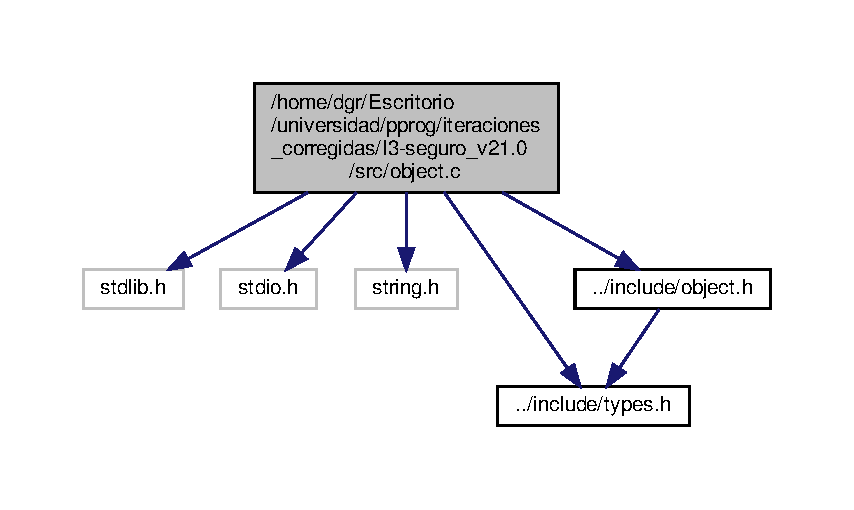
\includegraphics[width=350pt]{object_8c__incl}
\end{center}
\end{figure}
\subsection*{Data Structures}
\begin{DoxyCompactItemize}
\item 
struct \hyperlink{struct__Object}{\+\_\+\+Object}
\begin{DoxyCompactList}\small\item\em The object structure. \end{DoxyCompactList}\end{DoxyCompactItemize}
\subsection*{Functions}
\begin{DoxyCompactItemize}
\item 
\hyperlink{object_8h_a7f8bbcda919b65ce67f92fba08e0212f}{Object} $\ast$ \hyperlink{object_8c_abb0cd30fca5fbddf137c6c04df66bbc7}{object\+\_\+create} (\hyperlink{types_8h_a845e604fb28f7e3d97549da3448149d3}{Id} id)
\begin{DoxyCompactList}\small\item\em Create the object. \end{DoxyCompactList}\item 
\hyperlink{types_8h_a32c27cc471df37f4fc818d65de0a56c4}{S\+T\+A\+T\+US} \hyperlink{object_8c_a19d6d51fee809e3801893eefc789f4b4}{object\+\_\+destroy} (\hyperlink{object_8h_a7f8bbcda919b65ce67f92fba08e0212f}{Object} $\ast$object)
\begin{DoxyCompactList}\small\item\em free an object \end{DoxyCompactList}\item 
\hyperlink{types_8h_a32c27cc471df37f4fc818d65de0a56c4}{S\+T\+A\+T\+US} \hyperlink{object_8c_aff780fbe7b3a8280a05331918751e902}{object\+\_\+set\+\_\+dependency} (\hyperlink{object_8h_a7f8bbcda919b65ce67f92fba08e0212f}{Object} $\ast$object, \hyperlink{types_8h_a845e604fb28f7e3d97549da3448149d3}{Id} dependecy)
\begin{DoxyCompactList}\small\item\em set the dependency of an object \end{DoxyCompactList}\item 
\hyperlink{types_8h_a845e604fb28f7e3d97549da3448149d3}{Id} \hyperlink{object_8c_a9d40c68527b9f7b8264065914069b5e2}{object\+\_\+get\+\_\+dependency} (\hyperlink{object_8h_a7f8bbcda919b65ce67f92fba08e0212f}{Object} $\ast$object)
\begin{DoxyCompactList}\small\item\em get the dependency of an object \end{DoxyCompactList}\item 
\hyperlink{types_8h_a32c27cc471df37f4fc818d65de0a56c4}{S\+T\+A\+T\+US} \hyperlink{object_8c_a62e0c841696c92130d1c8cb8e706e5e6}{object\+\_\+set\+\_\+incompatible} (\hyperlink{object_8h_a7f8bbcda919b65ce67f92fba08e0212f}{Object} $\ast$object, \hyperlink{types_8h_a845e604fb28f7e3d97549da3448149d3}{Id} id)
\begin{DoxyCompactList}\small\item\em set the incompatible of an object \end{DoxyCompactList}\item 
\hyperlink{types_8h_a845e604fb28f7e3d97549da3448149d3}{Id} \hyperlink{object_8c_a1cf34d61291241d5bdc78c2549a76723}{object\+\_\+get\+\_\+incompatible} (\hyperlink{object_8h_a7f8bbcda919b65ce67f92fba08e0212f}{Object} $\ast$object)
\begin{DoxyCompactList}\small\item\em get the incompatible id of an object \end{DoxyCompactList}\item 
\hyperlink{types_8h_a32c27cc471df37f4fc818d65de0a56c4}{S\+T\+A\+T\+US} \hyperlink{object_8c_ac15dc062c857503ec0ca66037caffd80}{object\+\_\+set\+\_\+name} (\hyperlink{object_8h_a7f8bbcda919b65ce67f92fba08e0212f}{Object} $\ast$object, char $\ast$name)
\begin{DoxyCompactList}\small\item\em name the object \end{DoxyCompactList}\item 
\hyperlink{types_8h_a32c27cc471df37f4fc818d65de0a56c4}{S\+T\+A\+T\+US} \hyperlink{object_8c_a8af555646a21966db8d91da0f8fb02a3}{object\+\_\+turned} (\hyperlink{object_8h_a7f8bbcda919b65ce67f92fba08e0212f}{Object} $\ast$object, \hyperlink{types_8h_a3e5b8192e7d9ffaf3542f1210aec18dd}{B\+O\+OL} bool)
\begin{DoxyCompactList}\small\item\em set if the object is turned or not \end{DoxyCompactList}\item 
\hyperlink{types_8h_a3e5b8192e7d9ffaf3542f1210aec18dd}{B\+O\+OL} \hyperlink{object_8c_a90b9b53d70ac575fb0e611dbe19d11cc}{object\+\_\+get\+\_\+turned} (\hyperlink{object_8h_a7f8bbcda919b65ce67f92fba08e0212f}{Object} $\ast$object)
\begin{DoxyCompactList}\small\item\em used to know if the object is turned or not \end{DoxyCompactList}\item 
\hyperlink{types_8h_a32c27cc471df37f4fc818d65de0a56c4}{S\+T\+A\+T\+US} \hyperlink{object_8c_ae88627a8873d8f08fba9c0470a19cfc0}{object\+\_\+set\+\_\+description} (\hyperlink{object_8h_a7f8bbcda919b65ce67f92fba08e0212f}{Object} $\ast$object, char $\ast$description)
\begin{DoxyCompactList}\small\item\em set the description of an object \end{DoxyCompactList}\item 
\hyperlink{types_8h_a32c27cc471df37f4fc818d65de0a56c4}{S\+T\+A\+T\+US} \hyperlink{object_8c_a6e1125f2d373ef5e9421d0a83e7a0b02}{object\+\_\+set\+\_\+id} (\hyperlink{object_8h_a7f8bbcda919b65ce67f92fba08e0212f}{Object} $\ast$object, int id)
\begin{DoxyCompactList}\small\item\em set the id \end{DoxyCompactList}\item 
\hyperlink{types_8h_a32c27cc471df37f4fc818d65de0a56c4}{S\+T\+A\+T\+US} \hyperlink{object_8c_aa606c66f78eb70802b4cb324ee055522}{object\+\_\+set\+\_\+movable} (\hyperlink{object_8h_a7f8bbcda919b65ce67f92fba08e0212f}{Object} $\ast$object, \hyperlink{types_8h_a3e5b8192e7d9ffaf3542f1210aec18dd}{B\+O\+OL} bool)
\begin{DoxyCompactList}\small\item\em set the mavable of an object \end{DoxyCompactList}\item 
\hyperlink{types_8h_a3e5b8192e7d9ffaf3542f1210aec18dd}{B\+O\+OL} \hyperlink{object_8c_a013409023095272ee75cf6f13b680cf4}{object\+\_\+get\+\_\+movable} (\hyperlink{object_8h_a7f8bbcda919b65ce67f92fba08e0212f}{Object} $\ast$object)
\begin{DoxyCompactList}\small\item\em get the mavable of an object \end{DoxyCompactList}\item 
\hyperlink{types_8h_a32c27cc471df37f4fc818d65de0a56c4}{S\+T\+A\+T\+US} \hyperlink{object_8c_a56d6a523e4f6c4b6987d344d6ac7cdf8}{object\+\_\+set\+\_\+illuminate} (\hyperlink{object_8h_a7f8bbcda919b65ce67f92fba08e0212f}{Object} $\ast$object, \hyperlink{types_8h_a3e5b8192e7d9ffaf3542f1210aec18dd}{B\+O\+OL} bool)
\begin{DoxyCompactList}\small\item\em set the hability to iluminate of an object \end{DoxyCompactList}\item 
\hyperlink{types_8h_a3e5b8192e7d9ffaf3542f1210aec18dd}{B\+O\+OL} \hyperlink{object_8c_a98241a6ff6c17286b614eb5757bd3752}{object\+\_\+get\+\_\+illuminate} (\hyperlink{object_8h_a7f8bbcda919b65ce67f92fba08e0212f}{Object} $\ast$object)
\begin{DoxyCompactList}\small\item\em get the ilumination capacity of an object \end{DoxyCompactList}\item 
\hyperlink{types_8h_a32c27cc471df37f4fc818d65de0a56c4}{S\+T\+A\+T\+US} \hyperlink{object_8c_a81d1e8dbdbf2b76b1af44ed393c11479}{object\+\_\+set\+\_\+hidden} (\hyperlink{object_8h_a7f8bbcda919b65ce67f92fba08e0212f}{Object} $\ast$object, \hyperlink{types_8h_a3e5b8192e7d9ffaf3542f1210aec18dd}{B\+O\+OL} bool)
\begin{DoxyCompactList}\small\item\em set the hidden of an object \end{DoxyCompactList}\item 
\hyperlink{types_8h_a3e5b8192e7d9ffaf3542f1210aec18dd}{B\+O\+OL} \hyperlink{object_8c_a6171471129f33c873f5704e6309eee0d}{object\+\_\+get\+\_\+hidden} (\hyperlink{object_8h_a7f8bbcda919b65ce67f92fba08e0212f}{Object} $\ast$object)
\begin{DoxyCompactList}\small\item\em get the mavable of an object \end{DoxyCompactList}\item 
\hyperlink{types_8h_a32c27cc471df37f4fc818d65de0a56c4}{S\+T\+A\+T\+US} \hyperlink{object_8c_ab62e9c302600d7c9a61392fff1b06534}{object\+\_\+set\+\_\+open} (\hyperlink{object_8h_a7f8bbcda919b65ce67f92fba08e0212f}{Object} $\ast$object, \hyperlink{types_8h_a845e604fb28f7e3d97549da3448149d3}{Id} id)
\begin{DoxyCompactList}\small\item\em set the id of the link to open with an object \end{DoxyCompactList}\item 
\hyperlink{types_8h_a845e604fb28f7e3d97549da3448149d3}{Id} \hyperlink{object_8c_a49dbce205db36230c53fb0ccf0a73174}{object\+\_\+get\+\_\+open} (\hyperlink{object_8h_a7f8bbcda919b65ce67f92fba08e0212f}{Object} $\ast$object)
\begin{DoxyCompactList}\small\item\em get the id of the link that this object can open \end{DoxyCompactList}\item 
const char $\ast$ \hyperlink{object_8c_a19320eebcbbd38533a18c741b804b584}{object\+\_\+get\+\_\+name} (\hyperlink{object_8h_a7f8bbcda919b65ce67f92fba08e0212f}{Object} $\ast$object)
\begin{DoxyCompactList}\small\item\em get the name of the object \end{DoxyCompactList}\item 
const char $\ast$ \hyperlink{object_8c_a4b26ef1ec7057673899b58a5bf55f06a}{object\+\_\+get\+\_\+description} (\hyperlink{object_8h_a7f8bbcda919b65ce67f92fba08e0212f}{Object} $\ast$object)
\begin{DoxyCompactList}\small\item\em returns the description of an object \end{DoxyCompactList}\item 
\hyperlink{types_8h_a845e604fb28f7e3d97549da3448149d3}{Id} \hyperlink{object_8c_ac5af152381a21853c6a28cc120e8e7fe}{object\+\_\+get\+\_\+id} (\hyperlink{object_8h_a7f8bbcda919b65ce67f92fba08e0212f}{Object} $\ast$object)
\begin{DoxyCompactList}\small\item\em get the id of the object \end{DoxyCompactList}\item 
\hyperlink{types_8h_a32c27cc471df37f4fc818d65de0a56c4}{S\+T\+A\+T\+US} \hyperlink{object_8c_adebb77fb5d33fc70616ab3b2b64c27ce}{object\+\_\+print} (\hyperlink{object_8h_a7f8bbcda919b65ce67f92fba08e0212f}{Object} $\ast$object)
\begin{DoxyCompactList}\small\item\em print the information of the object on the screen \end{DoxyCompactList}\end{DoxyCompactItemize}


\subsection{Detailed Description}
add, load, and get spaces 

Store and set all the information about a player that is created, also can released the player.

Store and set all the information about an object that is created, also can release the object.

\begin{DoxyAuthor}{Author}
David Teófilo Garitagoitia Romero y José Manuel García Giráldez 
\end{DoxyAuthor}
\begin{DoxyVersion}{Version}
1.\+0 
\end{DoxyVersion}
\begin{DoxyDate}{Date}
06-\/02-\/2019 
\end{DoxyDate}
\begin{DoxyCopyright}{Copyright}
G\+NU Public License
\end{DoxyCopyright}
\begin{DoxyAuthor}{Author}
David Teófilo Garitagoitia Romero y José Manuel García Giráldez 
\end{DoxyAuthor}
\begin{DoxyVersion}{Version}
1.\+0 
\end{DoxyVersion}
\begin{DoxyDate}{Date}
07-\/02-\/2019 
\end{DoxyDate}
\begin{DoxyCopyright}{Copyright}
G\+NU Public License 
\end{DoxyCopyright}


\subsection{Function Documentation}
\mbox{\Hypertarget{object_8c_abb0cd30fca5fbddf137c6c04df66bbc7}\label{object_8c_abb0cd30fca5fbddf137c6c04df66bbc7}} 
\index{object.\+c@{object.\+c}!object\+\_\+create@{object\+\_\+create}}
\index{object\+\_\+create@{object\+\_\+create}!object.\+c@{object.\+c}}
\subsubsection{\texorpdfstring{object\+\_\+create()}{object\_create()}}
{\footnotesize\ttfamily \hyperlink{object_8h_a7f8bbcda919b65ce67f92fba08e0212f}{Object}$\ast$ object\+\_\+create (\begin{DoxyParamCaption}\item[{\hyperlink{types_8h_a845e604fb28f7e3d97549da3448149d3}{Id}}]{id }\end{DoxyParamCaption})}



Create the object. 

object\+\_\+create Create a object with a specific Id

\begin{DoxyDate}{Date}
07-\/02-\/2019 
\end{DoxyDate}
\begin{DoxyAuthor}{Author}
\+: José Manuel García Giráldez
\end{DoxyAuthor}

\begin{DoxyParams}{Parameters}
{\em id} & the id of the new object \\
\hline
\end{DoxyParams}
\begin{DoxyReturn}{Returns}
the new object that has been created 
\end{DoxyReturn}
\mbox{\Hypertarget{object_8c_a19d6d51fee809e3801893eefc789f4b4}\label{object_8c_a19d6d51fee809e3801893eefc789f4b4}} 
\index{object.\+c@{object.\+c}!object\+\_\+destroy@{object\+\_\+destroy}}
\index{object\+\_\+destroy@{object\+\_\+destroy}!object.\+c@{object.\+c}}
\subsubsection{\texorpdfstring{object\+\_\+destroy()}{object\_destroy()}}
{\footnotesize\ttfamily \hyperlink{types_8h_a32c27cc471df37f4fc818d65de0a56c4}{S\+T\+A\+T\+US} object\+\_\+destroy (\begin{DoxyParamCaption}\item[{\hyperlink{object_8h_a7f8bbcda919b65ce67f92fba08e0212f}{Object} $\ast$}]{object }\end{DoxyParamCaption})}



free an object 

object\+\_\+destroy free a especific object

\begin{DoxyDate}{Date}
07-\/02-\/2019 
\end{DoxyDate}
\begin{DoxyAuthor}{Author}
\+: José Manuel García Giráldez
\end{DoxyAuthor}

\begin{DoxyParams}{Parameters}
{\em object} & one object that has been created before \\
\hline
\end{DoxyParams}
\begin{DoxyReturn}{Returns}
E\+R\+R\+OR if there is an error, otherwise return OK 
\end{DoxyReturn}
\mbox{\Hypertarget{object_8c_a9d40c68527b9f7b8264065914069b5e2}\label{object_8c_a9d40c68527b9f7b8264065914069b5e2}} 
\index{object.\+c@{object.\+c}!object\+\_\+get\+\_\+dependency@{object\+\_\+get\+\_\+dependency}}
\index{object\+\_\+get\+\_\+dependency@{object\+\_\+get\+\_\+dependency}!object.\+c@{object.\+c}}
\subsubsection{\texorpdfstring{object\+\_\+get\+\_\+dependency()}{object\_get\_dependency()}}
{\footnotesize\ttfamily \hyperlink{types_8h_a845e604fb28f7e3d97549da3448149d3}{Id} object\+\_\+get\+\_\+dependency (\begin{DoxyParamCaption}\item[{\hyperlink{object_8h_a7f8bbcda919b65ce67f92fba08e0212f}{Object} $\ast$}]{object }\end{DoxyParamCaption})}



get the dependency of an object 

object\+\_\+get\+\_\+dependency

\begin{DoxyDate}{Date}
20-\/04-\/2020 
\end{DoxyDate}
\begin{DoxyAuthor}{Author}
\+: David Teófilo Garitagoitia Romero
\end{DoxyAuthor}

\begin{DoxyParams}{Parameters}
{\em object} & one object that has been created before \\
\hline
\end{DoxyParams}
\begin{DoxyReturn}{Returns}
Ok the dependency of the object 
\end{DoxyReturn}
\mbox{\Hypertarget{object_8c_a4b26ef1ec7057673899b58a5bf55f06a}\label{object_8c_a4b26ef1ec7057673899b58a5bf55f06a}} 
\index{object.\+c@{object.\+c}!object\+\_\+get\+\_\+description@{object\+\_\+get\+\_\+description}}
\index{object\+\_\+get\+\_\+description@{object\+\_\+get\+\_\+description}!object.\+c@{object.\+c}}
\subsubsection{\texorpdfstring{object\+\_\+get\+\_\+description()}{object\_get\_description()}}
{\footnotesize\ttfamily const char$\ast$ object\+\_\+get\+\_\+description (\begin{DoxyParamCaption}\item[{\hyperlink{object_8h_a7f8bbcda919b65ce67f92fba08e0212f}{Object} $\ast$}]{object }\end{DoxyParamCaption})}



returns the description of an object 

object\+\_\+get\+\_\+description

\begin{DoxyDate}{Date}
17-\/02-\/2019 
\end{DoxyDate}
\begin{DoxyAuthor}{Author}
\+: David Teófilo Garitagoitia Romero
\end{DoxyAuthor}

\begin{DoxyParams}{Parameters}
{\em object} & one object that has been created before \\
\hline
\end{DoxyParams}
\begin{DoxyReturn}{Returns}
the description of an object 
\end{DoxyReturn}
\mbox{\Hypertarget{object_8c_a6171471129f33c873f5704e6309eee0d}\label{object_8c_a6171471129f33c873f5704e6309eee0d}} 
\index{object.\+c@{object.\+c}!object\+\_\+get\+\_\+hidden@{object\+\_\+get\+\_\+hidden}}
\index{object\+\_\+get\+\_\+hidden@{object\+\_\+get\+\_\+hidden}!object.\+c@{object.\+c}}
\subsubsection{\texorpdfstring{object\+\_\+get\+\_\+hidden()}{object\_get\_hidden()}}
{\footnotesize\ttfamily \hyperlink{types_8h_a3e5b8192e7d9ffaf3542f1210aec18dd}{B\+O\+OL} object\+\_\+get\+\_\+hidden (\begin{DoxyParamCaption}\item[{\hyperlink{object_8h_a7f8bbcda919b65ce67f92fba08e0212f}{Object} $\ast$}]{object }\end{DoxyParamCaption})}



get the mavable of an object 

object\+\_\+get\+\_\+movable

\begin{DoxyDate}{Date}
20-\/04-\/2020 
\end{DoxyDate}
\begin{DoxyAuthor}{Author}
\+: David Teófilo Garitagoitia Romero
\end{DoxyAuthor}

\begin{DoxyParams}{Parameters}
{\em object} & one object that has been created before \\
\hline
\end{DoxyParams}
\begin{DoxyReturn}{Returns}
the hidden of an object 
\end{DoxyReturn}
\mbox{\Hypertarget{object_8c_ac5af152381a21853c6a28cc120e8e7fe}\label{object_8c_ac5af152381a21853c6a28cc120e8e7fe}} 
\index{object.\+c@{object.\+c}!object\+\_\+get\+\_\+id@{object\+\_\+get\+\_\+id}}
\index{object\+\_\+get\+\_\+id@{object\+\_\+get\+\_\+id}!object.\+c@{object.\+c}}
\subsubsection{\texorpdfstring{object\+\_\+get\+\_\+id()}{object\_get\_id()}}
{\footnotesize\ttfamily \hyperlink{types_8h_a845e604fb28f7e3d97549da3448149d3}{Id} object\+\_\+get\+\_\+id (\begin{DoxyParamCaption}\item[{\hyperlink{object_8h_a7f8bbcda919b65ce67f92fba08e0212f}{Object} $\ast$}]{object }\end{DoxyParamCaption})}



get the id of the object 

object\+\_\+get\+\_\+id

\begin{DoxyDate}{Date}
07-\/02-\/2019 
\end{DoxyDate}
\begin{DoxyAuthor}{Author}
\+: José Manuel García Giráldez
\end{DoxyAuthor}

\begin{DoxyParams}{Parameters}
{\em object} & one object that has been created before \\
\hline
\end{DoxyParams}
\begin{DoxyReturn}{Returns}
object-\/$>$id the id of the object we enter 
\end{DoxyReturn}
\mbox{\Hypertarget{object_8c_a98241a6ff6c17286b614eb5757bd3752}\label{object_8c_a98241a6ff6c17286b614eb5757bd3752}} 
\index{object.\+c@{object.\+c}!object\+\_\+get\+\_\+illuminate@{object\+\_\+get\+\_\+illuminate}}
\index{object\+\_\+get\+\_\+illuminate@{object\+\_\+get\+\_\+illuminate}!object.\+c@{object.\+c}}
\subsubsection{\texorpdfstring{object\+\_\+get\+\_\+illuminate()}{object\_get\_illuminate()}}
{\footnotesize\ttfamily \hyperlink{types_8h_a3e5b8192e7d9ffaf3542f1210aec18dd}{B\+O\+OL} object\+\_\+get\+\_\+illuminate (\begin{DoxyParamCaption}\item[{\hyperlink{object_8h_a7f8bbcda919b65ce67f92fba08e0212f}{Object} $\ast$}]{object }\end{DoxyParamCaption})}



get the ilumination capacity of an object 

object\+\_\+get\+\_\+ilumination

\begin{DoxyDate}{Date}
20-\/04-\/2020 
\end{DoxyDate}
\begin{DoxyAuthor}{Author}
\+: David Teófilo Garitagoitia Romero
\end{DoxyAuthor}

\begin{DoxyParams}{Parameters}
{\em object} & one object that has been created before \\
\hline
\end{DoxyParams}
\begin{DoxyReturn}{Returns}
true if the object can iluminate, false otherwise 
\end{DoxyReturn}
\mbox{\Hypertarget{object_8c_a1cf34d61291241d5bdc78c2549a76723}\label{object_8c_a1cf34d61291241d5bdc78c2549a76723}} 
\index{object.\+c@{object.\+c}!object\+\_\+get\+\_\+incompatible@{object\+\_\+get\+\_\+incompatible}}
\index{object\+\_\+get\+\_\+incompatible@{object\+\_\+get\+\_\+incompatible}!object.\+c@{object.\+c}}
\subsubsection{\texorpdfstring{object\+\_\+get\+\_\+incompatible()}{object\_get\_incompatible()}}
{\footnotesize\ttfamily \hyperlink{types_8h_a845e604fb28f7e3d97549da3448149d3}{Id} object\+\_\+get\+\_\+incompatible (\begin{DoxyParamCaption}\item[{\hyperlink{object_8h_a7f8bbcda919b65ce67f92fba08e0212f}{Object} $\ast$}]{object }\end{DoxyParamCaption})}



get the incompatible id of an object 

object\+\_\+get\+\_\+incompatible

\begin{DoxyDate}{Date}
20-\/04-\/2020 
\end{DoxyDate}
\begin{DoxyAuthor}{Author}
\+: David Teófilo Garitagoitia Romero
\end{DoxyAuthor}

\begin{DoxyParams}{Parameters}
{\em object} & one object that has been created before \\
\hline
\end{DoxyParams}
\begin{DoxyReturn}{Returns}
the id of the incompatible id 
\end{DoxyReturn}
\mbox{\Hypertarget{object_8c_a013409023095272ee75cf6f13b680cf4}\label{object_8c_a013409023095272ee75cf6f13b680cf4}} 
\index{object.\+c@{object.\+c}!object\+\_\+get\+\_\+movable@{object\+\_\+get\+\_\+movable}}
\index{object\+\_\+get\+\_\+movable@{object\+\_\+get\+\_\+movable}!object.\+c@{object.\+c}}
\subsubsection{\texorpdfstring{object\+\_\+get\+\_\+movable()}{object\_get\_movable()}}
{\footnotesize\ttfamily \hyperlink{types_8h_a3e5b8192e7d9ffaf3542f1210aec18dd}{B\+O\+OL} object\+\_\+get\+\_\+movable (\begin{DoxyParamCaption}\item[{\hyperlink{object_8h_a7f8bbcda919b65ce67f92fba08e0212f}{Object} $\ast$}]{object }\end{DoxyParamCaption})}



get the mavable of an object 

object\+\_\+get\+\_\+movable

\begin{DoxyDate}{Date}
20-\/04-\/2020 
\end{DoxyDate}
\begin{DoxyAuthor}{Author}
\+: David Teófilo Garitagoitia Romero
\end{DoxyAuthor}

\begin{DoxyParams}{Parameters}
{\em object} & one object that has been created before \\
\hline
\end{DoxyParams}
\begin{DoxyReturn}{Returns}
return the movable of an object 
\end{DoxyReturn}
\mbox{\Hypertarget{object_8c_a19320eebcbbd38533a18c741b804b584}\label{object_8c_a19320eebcbbd38533a18c741b804b584}} 
\index{object.\+c@{object.\+c}!object\+\_\+get\+\_\+name@{object\+\_\+get\+\_\+name}}
\index{object\+\_\+get\+\_\+name@{object\+\_\+get\+\_\+name}!object.\+c@{object.\+c}}
\subsubsection{\texorpdfstring{object\+\_\+get\+\_\+name()}{object\_get\_name()}}
{\footnotesize\ttfamily const char$\ast$ object\+\_\+get\+\_\+name (\begin{DoxyParamCaption}\item[{\hyperlink{object_8h_a7f8bbcda919b65ce67f92fba08e0212f}{Object} $\ast$}]{object }\end{DoxyParamCaption})}



get the name of the object 

object\+\_\+get\+\_\+name

\begin{DoxyDate}{Date}
07-\/02-\/2019 
\end{DoxyDate}
\begin{DoxyAuthor}{Author}
\+: David Teófilo Garitagoitia Romero
\end{DoxyAuthor}

\begin{DoxyParams}{Parameters}
{\em object} & one object that has been created before \\
\hline
\end{DoxyParams}
\begin{DoxyReturn}{Returns}
object-\/$>$name the name of the object we enter 
\end{DoxyReturn}
\mbox{\Hypertarget{object_8c_a49dbce205db36230c53fb0ccf0a73174}\label{object_8c_a49dbce205db36230c53fb0ccf0a73174}} 
\index{object.\+c@{object.\+c}!object\+\_\+get\+\_\+open@{object\+\_\+get\+\_\+open}}
\index{object\+\_\+get\+\_\+open@{object\+\_\+get\+\_\+open}!object.\+c@{object.\+c}}
\subsubsection{\texorpdfstring{object\+\_\+get\+\_\+open()}{object\_get\_open()}}
{\footnotesize\ttfamily \hyperlink{types_8h_a845e604fb28f7e3d97549da3448149d3}{Id} object\+\_\+get\+\_\+open (\begin{DoxyParamCaption}\item[{\hyperlink{object_8h_a7f8bbcda919b65ce67f92fba08e0212f}{Object} $\ast$}]{object }\end{DoxyParamCaption})}



get the id of the link that this object can open 

object\+\_\+get\+\_\+open

\begin{DoxyDate}{Date}
20-\/04-\/2020 
\end{DoxyDate}
\begin{DoxyAuthor}{Author}
\+: David Teófilo Garitagoitia Romero
\end{DoxyAuthor}

\begin{DoxyParams}{Parameters}
{\em object} & one object that has been created before \\
\hline
\end{DoxyParams}
\begin{DoxyReturn}{Returns}
the id of the link 
\end{DoxyReturn}
\mbox{\Hypertarget{object_8c_a90b9b53d70ac575fb0e611dbe19d11cc}\label{object_8c_a90b9b53d70ac575fb0e611dbe19d11cc}} 
\index{object.\+c@{object.\+c}!object\+\_\+get\+\_\+turned@{object\+\_\+get\+\_\+turned}}
\index{object\+\_\+get\+\_\+turned@{object\+\_\+get\+\_\+turned}!object.\+c@{object.\+c}}
\subsubsection{\texorpdfstring{object\+\_\+get\+\_\+turned()}{object\_get\_turned()}}
{\footnotesize\ttfamily \hyperlink{types_8h_a3e5b8192e7d9ffaf3542f1210aec18dd}{B\+O\+OL} object\+\_\+get\+\_\+turned (\begin{DoxyParamCaption}\item[{\hyperlink{object_8h_a7f8bbcda919b65ce67f92fba08e0212f}{Object} $\ast$}]{object }\end{DoxyParamCaption})}



used to know if the object is turned or not 

object\+\_\+get\+\_\+turned

\begin{DoxyDate}{Date}
20-\/04-\/2020 
\end{DoxyDate}
\begin{DoxyAuthor}{Author}
\+: David Teófilo Garitagoitia Romero
\end{DoxyAuthor}

\begin{DoxyParams}{Parameters}
{\em object} & one object that has been created before \\
\hline
\end{DoxyParams}
\begin{DoxyReturn}{Returns}
True if the object is turned on 
\end{DoxyReturn}
\mbox{\Hypertarget{object_8c_adebb77fb5d33fc70616ab3b2b64c27ce}\label{object_8c_adebb77fb5d33fc70616ab3b2b64c27ce}} 
\index{object.\+c@{object.\+c}!object\+\_\+print@{object\+\_\+print}}
\index{object\+\_\+print@{object\+\_\+print}!object.\+c@{object.\+c}}
\subsubsection{\texorpdfstring{object\+\_\+print()}{object\_print()}}
{\footnotesize\ttfamily \hyperlink{types_8h_a32c27cc471df37f4fc818d65de0a56c4}{S\+T\+A\+T\+US} object\+\_\+print (\begin{DoxyParamCaption}\item[{\hyperlink{object_8h_a7f8bbcda919b65ce67f92fba08e0212f}{Object} $\ast$}]{object }\end{DoxyParamCaption})}



print the information of the object on the screen 

object\+\_\+print

\begin{DoxyDate}{Date}
07-\/02-\/2019 
\end{DoxyDate}
\begin{DoxyAuthor}{Author}
\+: David Teófilo Garitagoitia Romero
\end{DoxyAuthor}

\begin{DoxyParams}{Parameters}
{\em object} & one object that has been created before \\
\hline
\end{DoxyParams}
\begin{DoxyReturn}{Returns}
E\+R\+R\+OR if there is an error, otherwise return OK 
\end{DoxyReturn}
\mbox{\Hypertarget{object_8c_aff780fbe7b3a8280a05331918751e902}\label{object_8c_aff780fbe7b3a8280a05331918751e902}} 
\index{object.\+c@{object.\+c}!object\+\_\+set\+\_\+dependency@{object\+\_\+set\+\_\+dependency}}
\index{object\+\_\+set\+\_\+dependency@{object\+\_\+set\+\_\+dependency}!object.\+c@{object.\+c}}
\subsubsection{\texorpdfstring{object\+\_\+set\+\_\+dependency()}{object\_set\_dependency()}}
{\footnotesize\ttfamily \hyperlink{types_8h_a32c27cc471df37f4fc818d65de0a56c4}{S\+T\+A\+T\+US} object\+\_\+set\+\_\+dependency (\begin{DoxyParamCaption}\item[{\hyperlink{object_8h_a7f8bbcda919b65ce67f92fba08e0212f}{Object} $\ast$}]{object,  }\item[{\hyperlink{types_8h_a845e604fb28f7e3d97549da3448149d3}{Id}}]{dependency }\end{DoxyParamCaption})}



set the dependency of an object 

object\+\_\+set\+\_\+dependency

\begin{DoxyDate}{Date}
20-\/04-\/2020 
\end{DoxyDate}
\begin{DoxyAuthor}{Author}
\+: David Teófilo Garitagoitia Romero
\end{DoxyAuthor}

\begin{DoxyParams}{Parameters}
{\em object} & one object that has been created before \\
\hline
{\em dependency} & the id of the dependency \\
\hline
\end{DoxyParams}
\begin{DoxyReturn}{Returns}
Ok if there is no error, false otherwise 
\end{DoxyReturn}
\mbox{\Hypertarget{object_8c_ae88627a8873d8f08fba9c0470a19cfc0}\label{object_8c_ae88627a8873d8f08fba9c0470a19cfc0}} 
\index{object.\+c@{object.\+c}!object\+\_\+set\+\_\+description@{object\+\_\+set\+\_\+description}}
\index{object\+\_\+set\+\_\+description@{object\+\_\+set\+\_\+description}!object.\+c@{object.\+c}}
\subsubsection{\texorpdfstring{object\+\_\+set\+\_\+description()}{object\_set\_description()}}
{\footnotesize\ttfamily \hyperlink{types_8h_a32c27cc471df37f4fc818d65de0a56c4}{S\+T\+A\+T\+US} object\+\_\+set\+\_\+description (\begin{DoxyParamCaption}\item[{\hyperlink{object_8h_a7f8bbcda919b65ce67f92fba08e0212f}{Object} $\ast$}]{object,  }\item[{char $\ast$}]{description }\end{DoxyParamCaption})}



set the description of an object 

object\+\_\+set\+\_\+description

\begin{DoxyDate}{Date}
17-\/02-\/2019 
\end{DoxyDate}
\begin{DoxyAuthor}{Author}
\+: David Teófilo Garitagoitia Romero
\end{DoxyAuthor}

\begin{DoxyParams}{Parameters}
{\em object} & one object that has been created before \\
\hline
{\em description} & the description we want to insert in the object \\
\hline
\end{DoxyParams}
\begin{DoxyReturn}{Returns}
E\+R\+R\+OR if there is an error, otherwise return OK 
\end{DoxyReturn}
\mbox{\Hypertarget{object_8c_a81d1e8dbdbf2b76b1af44ed393c11479}\label{object_8c_a81d1e8dbdbf2b76b1af44ed393c11479}} 
\index{object.\+c@{object.\+c}!object\+\_\+set\+\_\+hidden@{object\+\_\+set\+\_\+hidden}}
\index{object\+\_\+set\+\_\+hidden@{object\+\_\+set\+\_\+hidden}!object.\+c@{object.\+c}}
\subsubsection{\texorpdfstring{object\+\_\+set\+\_\+hidden()}{object\_set\_hidden()}}
{\footnotesize\ttfamily \hyperlink{types_8h_a32c27cc471df37f4fc818d65de0a56c4}{S\+T\+A\+T\+US} object\+\_\+set\+\_\+hidden (\begin{DoxyParamCaption}\item[{\hyperlink{object_8h_a7f8bbcda919b65ce67f92fba08e0212f}{Object} $\ast$}]{object,  }\item[{\hyperlink{types_8h_a3e5b8192e7d9ffaf3542f1210aec18dd}{B\+O\+OL}}]{bool }\end{DoxyParamCaption})}



set the hidden of an object 

object\+\_\+set\+\_\+hidden

\begin{DoxyDate}{Date}
20-\/04-\/2020 
\end{DoxyDate}
\begin{DoxyAuthor}{Author}
\+: David Teófilo Garitagoitia Romero
\end{DoxyAuthor}

\begin{DoxyParams}{Parameters}
{\em object} & one object that has been created before \\
\hline
{\em bool} & true or false \\
\hline
\end{DoxyParams}
\begin{DoxyReturn}{Returns}
Ok if there is no error, false otherwise 
\end{DoxyReturn}
\mbox{\Hypertarget{object_8c_a6e1125f2d373ef5e9421d0a83e7a0b02}\label{object_8c_a6e1125f2d373ef5e9421d0a83e7a0b02}} 
\index{object.\+c@{object.\+c}!object\+\_\+set\+\_\+id@{object\+\_\+set\+\_\+id}}
\index{object\+\_\+set\+\_\+id@{object\+\_\+set\+\_\+id}!object.\+c@{object.\+c}}
\subsubsection{\texorpdfstring{object\+\_\+set\+\_\+id()}{object\_set\_id()}}
{\footnotesize\ttfamily \hyperlink{types_8h_a32c27cc471df37f4fc818d65de0a56c4}{S\+T\+A\+T\+US} object\+\_\+set\+\_\+id (\begin{DoxyParamCaption}\item[{\hyperlink{object_8h_a7f8bbcda919b65ce67f92fba08e0212f}{Object} $\ast$}]{object,  }\item[{int}]{id }\end{DoxyParamCaption})}



set the id 

object\+\_\+set\+\_\+id

\begin{DoxyDate}{Date}
07-\/02-\/2019 
\end{DoxyDate}
\begin{DoxyAuthor}{Author}
\+: David Teófilo Garitagoitia Romero
\end{DoxyAuthor}

\begin{DoxyParams}{Parameters}
{\em object} & one object that has been created before \\
\hline
{\em id} & the id that the object will have \\
\hline
\end{DoxyParams}
\begin{DoxyReturn}{Returns}
E\+R\+R\+OR if there is an error, otherwise return OK 
\end{DoxyReturn}
\mbox{\Hypertarget{object_8c_a56d6a523e4f6c4b6987d344d6ac7cdf8}\label{object_8c_a56d6a523e4f6c4b6987d344d6ac7cdf8}} 
\index{object.\+c@{object.\+c}!object\+\_\+set\+\_\+illuminate@{object\+\_\+set\+\_\+illuminate}}
\index{object\+\_\+set\+\_\+illuminate@{object\+\_\+set\+\_\+illuminate}!object.\+c@{object.\+c}}
\subsubsection{\texorpdfstring{object\+\_\+set\+\_\+illuminate()}{object\_set\_illuminate()}}
{\footnotesize\ttfamily \hyperlink{types_8h_a32c27cc471df37f4fc818d65de0a56c4}{S\+T\+A\+T\+US} object\+\_\+set\+\_\+illuminate (\begin{DoxyParamCaption}\item[{\hyperlink{object_8h_a7f8bbcda919b65ce67f92fba08e0212f}{Object} $\ast$}]{object,  }\item[{\hyperlink{types_8h_a3e5b8192e7d9ffaf3542f1210aec18dd}{B\+O\+OL}}]{bool }\end{DoxyParamCaption})}



set the hability to iluminate of an object 

object\+\_\+set\+\_\+iluminate

\begin{DoxyDate}{Date}
20-\/04-\/2020 
\end{DoxyDate}
\begin{DoxyAuthor}{Author}
\+: David Teófilo Garitagoitia Romero
\end{DoxyAuthor}

\begin{DoxyParams}{Parameters}
{\em object} & one object that has been created before \\
\hline
{\em bool} & true or false \\
\hline
\end{DoxyParams}
\begin{DoxyReturn}{Returns}
Ok if there is no error, false otherwise 
\end{DoxyReturn}
\mbox{\Hypertarget{object_8c_a62e0c841696c92130d1c8cb8e706e5e6}\label{object_8c_a62e0c841696c92130d1c8cb8e706e5e6}} 
\index{object.\+c@{object.\+c}!object\+\_\+set\+\_\+incompatible@{object\+\_\+set\+\_\+incompatible}}
\index{object\+\_\+set\+\_\+incompatible@{object\+\_\+set\+\_\+incompatible}!object.\+c@{object.\+c}}
\subsubsection{\texorpdfstring{object\+\_\+set\+\_\+incompatible()}{object\_set\_incompatible()}}
{\footnotesize\ttfamily \hyperlink{types_8h_a32c27cc471df37f4fc818d65de0a56c4}{S\+T\+A\+T\+US} object\+\_\+set\+\_\+incompatible (\begin{DoxyParamCaption}\item[{\hyperlink{object_8h_a7f8bbcda919b65ce67f92fba08e0212f}{Object} $\ast$}]{object,  }\item[{\hyperlink{types_8h_a845e604fb28f7e3d97549da3448149d3}{Id}}]{id }\end{DoxyParamCaption})}



set the incompatible of an object 

object\+\_\+set\+\_\+incompatible

\begin{DoxyDate}{Date}
20-\/04-\/2020 
\end{DoxyDate}
\begin{DoxyAuthor}{Author}
\+: David Teófilo Garitagoitia Romero
\end{DoxyAuthor}

\begin{DoxyParams}{Parameters}
{\em object} & one object that has been created before \\
\hline
{\em id} & the id of the incompatible object \\
\hline
\end{DoxyParams}
\begin{DoxyReturn}{Returns}
Ok if there is no error, false otherwise 
\end{DoxyReturn}
\mbox{\Hypertarget{object_8c_aa606c66f78eb70802b4cb324ee055522}\label{object_8c_aa606c66f78eb70802b4cb324ee055522}} 
\index{object.\+c@{object.\+c}!object\+\_\+set\+\_\+movable@{object\+\_\+set\+\_\+movable}}
\index{object\+\_\+set\+\_\+movable@{object\+\_\+set\+\_\+movable}!object.\+c@{object.\+c}}
\subsubsection{\texorpdfstring{object\+\_\+set\+\_\+movable()}{object\_set\_movable()}}
{\footnotesize\ttfamily \hyperlink{types_8h_a32c27cc471df37f4fc818d65de0a56c4}{S\+T\+A\+T\+US} object\+\_\+set\+\_\+movable (\begin{DoxyParamCaption}\item[{\hyperlink{object_8h_a7f8bbcda919b65ce67f92fba08e0212f}{Object} $\ast$}]{object,  }\item[{\hyperlink{types_8h_a3e5b8192e7d9ffaf3542f1210aec18dd}{B\+O\+OL}}]{bool }\end{DoxyParamCaption})}



set the mavable of an object 

object\+\_\+set\+\_\+movable

\begin{DoxyDate}{Date}
20-\/04-\/2020 
\end{DoxyDate}
\begin{DoxyAuthor}{Author}
\+: David Teófilo Garitagoitia Romero
\end{DoxyAuthor}

\begin{DoxyParams}{Parameters}
{\em object} & one object that has been created before \\
\hline
{\em bool} & true or false \\
\hline
\end{DoxyParams}
\begin{DoxyReturn}{Returns}
Ok if there is no error, false otherwise 
\end{DoxyReturn}
\mbox{\Hypertarget{object_8c_ac15dc062c857503ec0ca66037caffd80}\label{object_8c_ac15dc062c857503ec0ca66037caffd80}} 
\index{object.\+c@{object.\+c}!object\+\_\+set\+\_\+name@{object\+\_\+set\+\_\+name}}
\index{object\+\_\+set\+\_\+name@{object\+\_\+set\+\_\+name}!object.\+c@{object.\+c}}
\subsubsection{\texorpdfstring{object\+\_\+set\+\_\+name()}{object\_set\_name()}}
{\footnotesize\ttfamily \hyperlink{types_8h_a32c27cc471df37f4fc818d65de0a56c4}{S\+T\+A\+T\+US} object\+\_\+set\+\_\+name (\begin{DoxyParamCaption}\item[{\hyperlink{object_8h_a7f8bbcda919b65ce67f92fba08e0212f}{Object} $\ast$}]{object,  }\item[{char $\ast$}]{name }\end{DoxyParamCaption})}



name the object 

object\+\_\+set\+\_\+name

\begin{DoxyDate}{Date}
07-\/02-\/2019 
\end{DoxyDate}
\begin{DoxyAuthor}{Author}
\+: David Teófilo Garitagoitia Romero
\end{DoxyAuthor}

\begin{DoxyParams}{Parameters}
{\em object} & one object that has been created before \\
\hline
{\em name} & the name that the object will have \\
\hline
\end{DoxyParams}
\begin{DoxyReturn}{Returns}
E\+R\+R\+OR if there is an error, otherwise return OK 
\end{DoxyReturn}
\mbox{\Hypertarget{object_8c_ab62e9c302600d7c9a61392fff1b06534}\label{object_8c_ab62e9c302600d7c9a61392fff1b06534}} 
\index{object.\+c@{object.\+c}!object\+\_\+set\+\_\+open@{object\+\_\+set\+\_\+open}}
\index{object\+\_\+set\+\_\+open@{object\+\_\+set\+\_\+open}!object.\+c@{object.\+c}}
\subsubsection{\texorpdfstring{object\+\_\+set\+\_\+open()}{object\_set\_open()}}
{\footnotesize\ttfamily \hyperlink{types_8h_a32c27cc471df37f4fc818d65de0a56c4}{S\+T\+A\+T\+US} object\+\_\+set\+\_\+open (\begin{DoxyParamCaption}\item[{\hyperlink{object_8h_a7f8bbcda919b65ce67f92fba08e0212f}{Object} $\ast$}]{object,  }\item[{\hyperlink{types_8h_a845e604fb28f7e3d97549da3448149d3}{Id}}]{id }\end{DoxyParamCaption})}



set the id of the link to open with an object 

object\+\_\+set\+\_\+opem

\begin{DoxyDate}{Date}
20-\/04-\/2020 
\end{DoxyDate}
\begin{DoxyAuthor}{Author}
\+: David Teófilo Garitagoitia Romero
\end{DoxyAuthor}

\begin{DoxyParams}{Parameters}
{\em object} & one object that has been created before \\
\hline
{\em id} & the id of the link that can open \\
\hline
\end{DoxyParams}
\begin{DoxyReturn}{Returns}
Ok if there is no error, false otherwise 
\end{DoxyReturn}
\mbox{\Hypertarget{object_8c_a8af555646a21966db8d91da0f8fb02a3}\label{object_8c_a8af555646a21966db8d91da0f8fb02a3}} 
\index{object.\+c@{object.\+c}!object\+\_\+turned@{object\+\_\+turned}}
\index{object\+\_\+turned@{object\+\_\+turned}!object.\+c@{object.\+c}}
\subsubsection{\texorpdfstring{object\+\_\+turned()}{object\_turned()}}
{\footnotesize\ttfamily \hyperlink{types_8h_a32c27cc471df37f4fc818d65de0a56c4}{S\+T\+A\+T\+US} object\+\_\+turned (\begin{DoxyParamCaption}\item[{\hyperlink{object_8h_a7f8bbcda919b65ce67f92fba08e0212f}{Object} $\ast$}]{object,  }\item[{\hyperlink{types_8h_a3e5b8192e7d9ffaf3542f1210aec18dd}{B\+O\+OL}}]{bool }\end{DoxyParamCaption})}



set if the object is turned or not 

object\+\_\+turned

\begin{DoxyDate}{Date}
20-\/04-\/2020 
\end{DoxyDate}
\begin{DoxyAuthor}{Author}
\+: David Teófilo Garitagoitia Romero
\end{DoxyAuthor}

\begin{DoxyParams}{Parameters}
{\em object} & one object that has been created before \\
\hline
{\em bool} & true or false \\
\hline
\end{DoxyParams}
\begin{DoxyReturn}{Returns}
Ok if there is no error, false otherwise 
\end{DoxyReturn}

\hypertarget{object__test_8c}{}\section{src/object\+\_\+test.c File Reference}
\label{object__test_8c}\index{src/object\+\_\+test.\+c@{src/object\+\_\+test.\+c}}


test to see if object works correctly  


{\ttfamily \#include $<$stdio.\+h$>$}\newline
{\ttfamily \#include $<$string.\+h$>$}\newline
{\ttfamily \#include $<$stdlib.\+h$>$}\newline
{\ttfamily \#include \char`\"{}../include/object.\+h\char`\"{}}\newline
{\ttfamily \#include \char`\"{}../include/test.\+h\char`\"{}}\newline
{\ttfamily \#include \char`\"{}../include/object\+\_\+test.\+h\char`\"{}}\newline
Include dependency graph for object\+\_\+test.\+c\+:\nopagebreak
\begin{figure}[H]
\begin{center}
\leavevmode
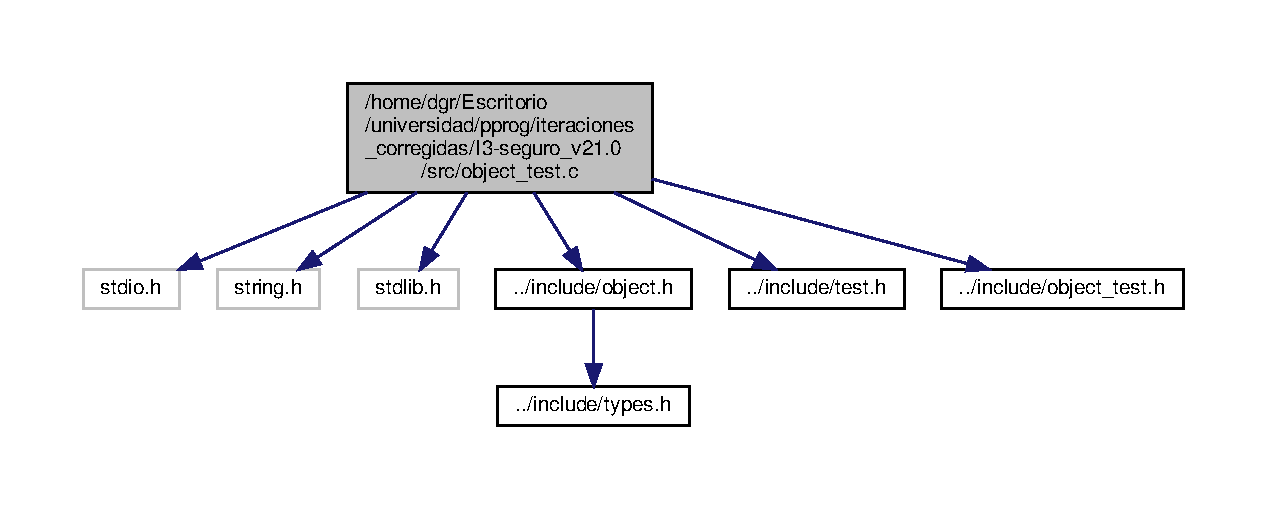
\includegraphics[width=350pt]{object__test_8c__incl}
\end{center}
\end{figure}
\subsection*{Macros}
\begin{DoxyCompactItemize}
\item 
\#define \hyperlink{object__test_8c_a2a77d2f2c5b698c69c19e1f8782bf709}{M\+A\+X\+\_\+\+T\+E\+S\+TS}~34
\begin{DoxyCompactList}\small\item\em maximum number of test \end{DoxyCompactList}\end{DoxyCompactItemize}
\subsection*{Functions}
\begin{DoxyCompactItemize}
\item 
int \hyperlink{object__test_8c_a3c04138a5bfe5d72780bb7e82a18e627}{main} (int argc, char $\ast$$\ast$argv)
\begin{DoxyCompactList}\small\item\em the main function of object\+\_\+test main \end{DoxyCompactList}\item 
void \hyperlink{object__test_8c_a3836d69f92ce7149d56bafcaec83f516}{test1\+\_\+object\+\_\+create} ()
\item 
void \hyperlink{object__test_8c_add54ab5e33a1b0a93e9ddcf73591bd9f}{test2\+\_\+object\+\_\+create} ()
\item 
void \hyperlink{object__test_8c_a818f180e2b7402835c6ac7ec0ba49f64}{test3\+\_\+object\+\_\+create} ()
\item 
void \hyperlink{object__test_8c_a781fa42f9f80e3906c01e62da67ffe60}{test4\+\_\+object\+\_\+create} ()
\item 
void \hyperlink{object__test_8c_a2f0dbf8e10011494c1ebc6749cbe98e8}{test5\+\_\+object\+\_\+create} ()
\item 
void \hyperlink{object__test_8c_ac8eaf663575fca548022f4bdad35dbd0}{test6\+\_\+object\+\_\+create} ()
\item 
void \hyperlink{object__test_8c_ad2d74fea18e3ea54d91cd2e23f5b49f1}{test7\+\_\+object\+\_\+create} ()
\item 
void \hyperlink{object__test_8c_a36cc6282195aa7ace8e870ffce9c5bbc}{test8\+\_\+object\+\_\+create} ()
\item 
void \hyperlink{object__test_8c_a8fbaf869a4764c7754332619d55eefd5}{test9\+\_\+object\+\_\+create} ()
\item 
void \hyperlink{object__test_8c_a74e25ad653c4a32b9922fff8e4f916fd}{test1\+\_\+object\+\_\+set\+\_\+name} ()
\item 
void \hyperlink{object__test_8c_acf42b7e7be91ede243f2aaa56c4c9347}{test2\+\_\+object\+\_\+set\+\_\+name} ()
\item 
void \hyperlink{object__test_8c_afb26b8c66d332354df8bfd57a8033b8f}{test1\+\_\+object\+\_\+set\+\_\+description} ()
\item 
void \hyperlink{object__test_8c_a65e32c3642c1d9207cdd84b134c616da}{test2\+\_\+object\+\_\+set\+\_\+description} ()
\item 
void \hyperlink{object__test_8c_afe180b78a201df7bc1629701db1d464c}{test1\+\_\+object\+\_\+get\+\_\+description} ()
\item 
void \hyperlink{object__test_8c_a35d9a40796133791c157c044ea1cef85}{test2\+\_\+object\+\_\+get\+\_\+description} ()
\item 
void \hyperlink{object__test_8c_aa88e9e9dab92ba9c58851d7a7a8415f0}{test1\+\_\+object\+\_\+get\+\_\+id} ()
\item 
void \hyperlink{object__test_8c_a1ff250f0f43297f57fcce1f3a6ae490b}{test2\+\_\+object\+\_\+get\+\_\+id} ()
\item 
void \hyperlink{object__test_8c_ad2411bc3cc47c9905e63a3d9c561d369}{test1\+\_\+object\+\_\+get\+\_\+name} ()
\item 
void \hyperlink{object__test_8c_abdfafbc7b8588d3dcdb05fd2beb2397e}{test2\+\_\+object\+\_\+get\+\_\+name} ()
\item 
void \hyperlink{object__test_8c_a093b7556c2271c532f607b6e7f15c36c}{test1\+\_\+object\+\_\+set\+\_\+movable} ()
\item 
void \hyperlink{object__test_8c_a2df3adcfcaef2fc447769d038de41895}{test2\+\_\+object\+\_\+set\+\_\+movable} ()
\item 
void \hyperlink{object__test_8c_a28605c20187056beac0c0e12a2a39fc3}{test1\+\_\+object\+\_\+get\+\_\+movable} ()
\item 
void \hyperlink{object__test_8c_a70a20d7dbb2cfdfd3c94572d083be5e5}{test2\+\_\+object\+\_\+get\+\_\+movable} ()
\item 
void \hyperlink{object__test_8c_aef1285f1a9ad407e927375aba038a706}{test1\+\_\+object\+\_\+set\+\_\+dependency} ()
\item 
void \hyperlink{object__test_8c_aa60a8195c4200bf68d77b34705a5fd40}{test2\+\_\+object\+\_\+set\+\_\+dependency} ()
\item 
void \hyperlink{object__test_8c_aff882e9769d27a86bd3ede47c1be29d4}{test1\+\_\+object\+\_\+get\+\_\+dependency} ()
\item 
void \hyperlink{object__test_8c_af8746713a9b762b1295bb1c4186260b8}{test2\+\_\+object\+\_\+get\+\_\+dependency} ()
\item 
void \hyperlink{object__test_8c_a54f1f4b62291243f6982bef4293d1ad6}{test1\+\_\+object\+\_\+set\+\_\+incompatible} ()
\item 
void \hyperlink{object__test_8c_ac5b76a6940bfdfa5e45fc60fafcb98e6}{test2\+\_\+object\+\_\+set\+\_\+incompatible} ()
\item 
void \hyperlink{object__test_8c_a918e86d4fc21c0f0c7ebd8f337415aa6}{test1\+\_\+object\+\_\+get\+\_\+incompatible} ()
\item 
void \hyperlink{object__test_8c_a7cd3b16d810720ff1c5c2ac646ab324e}{test2\+\_\+object\+\_\+get\+\_\+incompatible} ()
\item 
void \hyperlink{object__test_8c_a0986ab3c25b1bd5e93d269f1ba22c3b1}{test1\+\_\+object\+\_\+turned} ()
\item 
void \hyperlink{object__test_8c_a194f98fdeb81258e38ffe514f2d05601}{test2\+\_\+object\+\_\+turned} ()
\item 
void \hyperlink{object__test_8c_a9d4ea264164ea311c41d8664d83e0347}{test1\+\_\+object\+\_\+get\+\_\+turned} ()
\end{DoxyCompactItemize}


\subsection{Detailed Description}
test to see if object works correctly 

\begin{DoxyAuthor}{Author}
Daniel Cerrato Sánchez 
\end{DoxyAuthor}
\begin{DoxyVersion}{Version}
2.\+0 
\end{DoxyVersion}
\begin{DoxyDate}{Date}
10-\/06-\/2020 
\end{DoxyDate}
\begin{DoxyCopyright}{Copyright}
G\+NU Public License 
\end{DoxyCopyright}


\subsection{Macro Definition Documentation}
\mbox{\Hypertarget{object__test_8c_a2a77d2f2c5b698c69c19e1f8782bf709}\label{object__test_8c_a2a77d2f2c5b698c69c19e1f8782bf709}} 
\index{object\+\_\+test.\+c@{object\+\_\+test.\+c}!M\+A\+X\+\_\+\+T\+E\+S\+TS@{M\+A\+X\+\_\+\+T\+E\+S\+TS}}
\index{M\+A\+X\+\_\+\+T\+E\+S\+TS@{M\+A\+X\+\_\+\+T\+E\+S\+TS}!object\+\_\+test.\+c@{object\+\_\+test.\+c}}
\subsubsection{\texorpdfstring{M\+A\+X\+\_\+\+T\+E\+S\+TS}{MAX\_TESTS}}
{\footnotesize\ttfamily \#define M\+A\+X\+\_\+\+T\+E\+S\+TS~34}



maximum number of test 

Details. 

\subsection{Function Documentation}
\mbox{\Hypertarget{object__test_8c_a3c04138a5bfe5d72780bb7e82a18e627}\label{object__test_8c_a3c04138a5bfe5d72780bb7e82a18e627}} 
\index{object\+\_\+test.\+c@{object\+\_\+test.\+c}!main@{main}}
\index{main@{main}!object\+\_\+test.\+c@{object\+\_\+test.\+c}}
\subsubsection{\texorpdfstring{main()}{main()}}
{\footnotesize\ttfamily int main (\begin{DoxyParamCaption}\item[{int}]{argc,  }\item[{char $\ast$$\ast$}]{argv }\end{DoxyParamCaption})}



the main function of object\+\_\+test main 

\begin{DoxyDate}{Date}
10-\/06-\/2020 
\end{DoxyDate}
\begin{DoxyAuthor}{Author}
Daniel Cerrato Sánchez 
\end{DoxyAuthor}
\begin{DoxyReturn}{Returns}

\end{DoxyReturn}
\mbox{\Hypertarget{object__test_8c_a3836d69f92ce7149d56bafcaec83f516}\label{object__test_8c_a3836d69f92ce7149d56bafcaec83f516}} 
\index{object\+\_\+test.\+c@{object\+\_\+test.\+c}!test1\+\_\+object\+\_\+create@{test1\+\_\+object\+\_\+create}}
\index{test1\+\_\+object\+\_\+create@{test1\+\_\+object\+\_\+create}!object\+\_\+test.\+c@{object\+\_\+test.\+c}}
\subsubsection{\texorpdfstring{test1\+\_\+object\+\_\+create()}{test1\_object\_create()}}
{\footnotesize\ttfamily void test1\+\_\+object\+\_\+create (\begin{DoxyParamCaption}{ }\end{DoxyParamCaption})}

\begin{DoxyRefDesc}{Test}
\item[\hyperlink{test__test000165}{Test}]Test the function of creating an object \end{DoxyRefDesc}
\begin{DoxyPrecond}{Precondition}
An id as parameter 
\end{DoxyPrecond}
\begin{DoxyPostcond}{Postcondition}
A non-\/null pointer to the created object 
\end{DoxyPostcond}
\mbox{\Hypertarget{object__test_8c_aff882e9769d27a86bd3ede47c1be29d4}\label{object__test_8c_aff882e9769d27a86bd3ede47c1be29d4}} 
\index{object\+\_\+test.\+c@{object\+\_\+test.\+c}!test1\+\_\+object\+\_\+get\+\_\+dependency@{test1\+\_\+object\+\_\+get\+\_\+dependency}}
\index{test1\+\_\+object\+\_\+get\+\_\+dependency@{test1\+\_\+object\+\_\+get\+\_\+dependency}!object\+\_\+test.\+c@{object\+\_\+test.\+c}}
\subsubsection{\texorpdfstring{test1\+\_\+object\+\_\+get\+\_\+dependency()}{test1\_object\_get\_dependency()}}
{\footnotesize\ttfamily void test1\+\_\+object\+\_\+get\+\_\+dependency (\begin{DoxyParamCaption}{ }\end{DoxyParamCaption})}

\begin{DoxyRefDesc}{Test}
\item[\hyperlink{test__test000190}{Test}]Test the function to get dependency of an object \end{DoxyRefDesc}
\begin{DoxyPrecond}{Precondition}
The dependency you want to set and the object 
\end{DoxyPrecond}
\begin{DoxyPostcond}{Postcondition}
The output must be the dependency you set before 
\end{DoxyPostcond}
\mbox{\Hypertarget{object__test_8c_afe180b78a201df7bc1629701db1d464c}\label{object__test_8c_afe180b78a201df7bc1629701db1d464c}} 
\index{object\+\_\+test.\+c@{object\+\_\+test.\+c}!test1\+\_\+object\+\_\+get\+\_\+description@{test1\+\_\+object\+\_\+get\+\_\+description}}
\index{test1\+\_\+object\+\_\+get\+\_\+description@{test1\+\_\+object\+\_\+get\+\_\+description}!object\+\_\+test.\+c@{object\+\_\+test.\+c}}
\subsubsection{\texorpdfstring{test1\+\_\+object\+\_\+get\+\_\+description()}{test1\_object\_get\_description()}}
{\footnotesize\ttfamily void test1\+\_\+object\+\_\+get\+\_\+description (\begin{DoxyParamCaption}{ }\end{DoxyParamCaption})}

\begin{DoxyRefDesc}{Test}
\item[\hyperlink{test__test000178}{Test}]Test the function to get the description of an object \end{DoxyRefDesc}
\begin{DoxyPrecond}{Precondition}
The object is a non-\/\+N\+U\+LL pointer with correct description 
\end{DoxyPrecond}
\begin{DoxyPostcond}{Postcondition}
The comparison between the description and the phrase to compare must be 0 
\end{DoxyPostcond}
\mbox{\Hypertarget{object__test_8c_aa88e9e9dab92ba9c58851d7a7a8415f0}\label{object__test_8c_aa88e9e9dab92ba9c58851d7a7a8415f0}} 
\index{object\+\_\+test.\+c@{object\+\_\+test.\+c}!test1\+\_\+object\+\_\+get\+\_\+id@{test1\+\_\+object\+\_\+get\+\_\+id}}
\index{test1\+\_\+object\+\_\+get\+\_\+id@{test1\+\_\+object\+\_\+get\+\_\+id}!object\+\_\+test.\+c@{object\+\_\+test.\+c}}
\subsubsection{\texorpdfstring{test1\+\_\+object\+\_\+get\+\_\+id()}{test1\_object\_get\_id()}}
{\footnotesize\ttfamily void test1\+\_\+object\+\_\+get\+\_\+id (\begin{DoxyParamCaption}{ }\end{DoxyParamCaption})}

\begin{DoxyRefDesc}{Test}
\item[\hyperlink{test__test000180}{Test}]Test the function to get the id of an object \end{DoxyRefDesc}
\begin{DoxyPrecond}{Precondition}
The object is a non-\/\+N\+U\+LL pointer with correct id 
\end{DoxyPrecond}
\begin{DoxyPostcond}{Postcondition}
The output must be the correct id 
\end{DoxyPostcond}
\mbox{\Hypertarget{object__test_8c_a918e86d4fc21c0f0c7ebd8f337415aa6}\label{object__test_8c_a918e86d4fc21c0f0c7ebd8f337415aa6}} 
\index{object\+\_\+test.\+c@{object\+\_\+test.\+c}!test1\+\_\+object\+\_\+get\+\_\+incompatible@{test1\+\_\+object\+\_\+get\+\_\+incompatible}}
\index{test1\+\_\+object\+\_\+get\+\_\+incompatible@{test1\+\_\+object\+\_\+get\+\_\+incompatible}!object\+\_\+test.\+c@{object\+\_\+test.\+c}}
\subsubsection{\texorpdfstring{test1\+\_\+object\+\_\+get\+\_\+incompatible()}{test1\_object\_get\_incompatible()}}
{\footnotesize\ttfamily void test1\+\_\+object\+\_\+get\+\_\+incompatible (\begin{DoxyParamCaption}{ }\end{DoxyParamCaption})}

\begin{DoxyRefDesc}{Test}
\item[\hyperlink{test__test000194}{Test}]Test the function to get incompatible of an object \end{DoxyRefDesc}
\begin{DoxyPrecond}{Precondition}
The incompatible you want to set and the object 
\end{DoxyPrecond}
\begin{DoxyPostcond}{Postcondition}
The output must be the incompatible you set before 
\end{DoxyPostcond}
\mbox{\Hypertarget{object__test_8c_a28605c20187056beac0c0e12a2a39fc3}\label{object__test_8c_a28605c20187056beac0c0e12a2a39fc3}} 
\index{object\+\_\+test.\+c@{object\+\_\+test.\+c}!test1\+\_\+object\+\_\+get\+\_\+movable@{test1\+\_\+object\+\_\+get\+\_\+movable}}
\index{test1\+\_\+object\+\_\+get\+\_\+movable@{test1\+\_\+object\+\_\+get\+\_\+movable}!object\+\_\+test.\+c@{object\+\_\+test.\+c}}
\subsubsection{\texorpdfstring{test1\+\_\+object\+\_\+get\+\_\+movable()}{test1\_object\_get\_movable()}}
{\footnotesize\ttfamily void test1\+\_\+object\+\_\+get\+\_\+movable (\begin{DoxyParamCaption}{ }\end{DoxyParamCaption})}

\begin{DoxyRefDesc}{Test}
\item[\hyperlink{test__test000186}{Test}]Test the function to get movable of an object \end{DoxyRefDesc}
\begin{DoxyPrecond}{Precondition}
The movable you want to set and the object 
\end{DoxyPrecond}
\begin{DoxyPostcond}{Postcondition}
The output must be the movable you set before 
\end{DoxyPostcond}
\mbox{\Hypertarget{object__test_8c_ad2411bc3cc47c9905e63a3d9c561d369}\label{object__test_8c_ad2411bc3cc47c9905e63a3d9c561d369}} 
\index{object\+\_\+test.\+c@{object\+\_\+test.\+c}!test1\+\_\+object\+\_\+get\+\_\+name@{test1\+\_\+object\+\_\+get\+\_\+name}}
\index{test1\+\_\+object\+\_\+get\+\_\+name@{test1\+\_\+object\+\_\+get\+\_\+name}!object\+\_\+test.\+c@{object\+\_\+test.\+c}}
\subsubsection{\texorpdfstring{test1\+\_\+object\+\_\+get\+\_\+name()}{test1\_object\_get\_name()}}
{\footnotesize\ttfamily void test1\+\_\+object\+\_\+get\+\_\+name (\begin{DoxyParamCaption}{ }\end{DoxyParamCaption})}

\begin{DoxyRefDesc}{Test}
\item[\hyperlink{test__test000182}{Test}]Test the function to get the name of an object \end{DoxyRefDesc}
\begin{DoxyPrecond}{Precondition}
Object is a non-\/\+N\+U\+LL pointer with correct name 
\end{DoxyPrecond}
\begin{DoxyPostcond}{Postcondition}
The comparison between the name and the word to compare must be 0 
\end{DoxyPostcond}
\mbox{\Hypertarget{object__test_8c_a9d4ea264164ea311c41d8664d83e0347}\label{object__test_8c_a9d4ea264164ea311c41d8664d83e0347}} 
\index{object\+\_\+test.\+c@{object\+\_\+test.\+c}!test1\+\_\+object\+\_\+get\+\_\+turned@{test1\+\_\+object\+\_\+get\+\_\+turned}}
\index{test1\+\_\+object\+\_\+get\+\_\+turned@{test1\+\_\+object\+\_\+get\+\_\+turned}!object\+\_\+test.\+c@{object\+\_\+test.\+c}}
\subsubsection{\texorpdfstring{test1\+\_\+object\+\_\+get\+\_\+turned()}{test1\_object\_get\_turned()}}
{\footnotesize\ttfamily void test1\+\_\+object\+\_\+get\+\_\+turned (\begin{DoxyParamCaption}{ }\end{DoxyParamCaption})}

\begin{DoxyRefDesc}{Test}
\item[\hyperlink{test__test000198}{Test}]Test the function to get turned of an object \end{DoxyRefDesc}
\begin{DoxyPrecond}{Precondition}
The object and the turner 
\end{DoxyPrecond}
\begin{DoxyPostcond}{Postcondition}
The output must be the one you have written 
\end{DoxyPostcond}
\mbox{\Hypertarget{object__test_8c_aef1285f1a9ad407e927375aba038a706}\label{object__test_8c_aef1285f1a9ad407e927375aba038a706}} 
\index{object\+\_\+test.\+c@{object\+\_\+test.\+c}!test1\+\_\+object\+\_\+set\+\_\+dependency@{test1\+\_\+object\+\_\+set\+\_\+dependency}}
\index{test1\+\_\+object\+\_\+set\+\_\+dependency@{test1\+\_\+object\+\_\+set\+\_\+dependency}!object\+\_\+test.\+c@{object\+\_\+test.\+c}}
\subsubsection{\texorpdfstring{test1\+\_\+object\+\_\+set\+\_\+dependency()}{test1\_object\_set\_dependency()}}
{\footnotesize\ttfamily void test1\+\_\+object\+\_\+set\+\_\+dependency (\begin{DoxyParamCaption}{ }\end{DoxyParamCaption})}

\begin{DoxyRefDesc}{Test}
\item[\hyperlink{test__test000188}{Test}]Test the function to set dependency of an object \end{DoxyRefDesc}
\begin{DoxyPrecond}{Precondition}
The dependency atribute 
\end{DoxyPrecond}
\begin{DoxyPostcond}{Postcondition}
The output must be OK 
\end{DoxyPostcond}
\mbox{\Hypertarget{object__test_8c_afb26b8c66d332354df8bfd57a8033b8f}\label{object__test_8c_afb26b8c66d332354df8bfd57a8033b8f}} 
\index{object\+\_\+test.\+c@{object\+\_\+test.\+c}!test1\+\_\+object\+\_\+set\+\_\+description@{test1\+\_\+object\+\_\+set\+\_\+description}}
\index{test1\+\_\+object\+\_\+set\+\_\+description@{test1\+\_\+object\+\_\+set\+\_\+description}!object\+\_\+test.\+c@{object\+\_\+test.\+c}}
\subsubsection{\texorpdfstring{test1\+\_\+object\+\_\+set\+\_\+description()}{test1\_object\_set\_description()}}
{\footnotesize\ttfamily void test1\+\_\+object\+\_\+set\+\_\+description (\begin{DoxyParamCaption}{ }\end{DoxyParamCaption})}

\begin{DoxyRefDesc}{Test}
\item[\hyperlink{test__test000176}{Test}]Test the function to change the description of an object \end{DoxyRefDesc}
\begin{DoxyPrecond}{Precondition}
The object is a non-\/\+N\+U\+LL pointer, the description is correct 
\end{DoxyPrecond}
\begin{DoxyPostcond}{Postcondition}
The output must be OK 
\end{DoxyPostcond}
\mbox{\Hypertarget{object__test_8c_a54f1f4b62291243f6982bef4293d1ad6}\label{object__test_8c_a54f1f4b62291243f6982bef4293d1ad6}} 
\index{object\+\_\+test.\+c@{object\+\_\+test.\+c}!test1\+\_\+object\+\_\+set\+\_\+incompatible@{test1\+\_\+object\+\_\+set\+\_\+incompatible}}
\index{test1\+\_\+object\+\_\+set\+\_\+incompatible@{test1\+\_\+object\+\_\+set\+\_\+incompatible}!object\+\_\+test.\+c@{object\+\_\+test.\+c}}
\subsubsection{\texorpdfstring{test1\+\_\+object\+\_\+set\+\_\+incompatible()}{test1\_object\_set\_incompatible()}}
{\footnotesize\ttfamily void test1\+\_\+object\+\_\+set\+\_\+incompatible (\begin{DoxyParamCaption}{ }\end{DoxyParamCaption})}

\begin{DoxyRefDesc}{Test}
\item[\hyperlink{test__test000192}{Test}]Test the function to set incompatible of an object \end{DoxyRefDesc}
\begin{DoxyPrecond}{Precondition}
The incompatible atribute 
\end{DoxyPrecond}
\begin{DoxyPostcond}{Postcondition}
The output must be OK 
\end{DoxyPostcond}
\mbox{\Hypertarget{object__test_8c_a093b7556c2271c532f607b6e7f15c36c}\label{object__test_8c_a093b7556c2271c532f607b6e7f15c36c}} 
\index{object\+\_\+test.\+c@{object\+\_\+test.\+c}!test1\+\_\+object\+\_\+set\+\_\+movable@{test1\+\_\+object\+\_\+set\+\_\+movable}}
\index{test1\+\_\+object\+\_\+set\+\_\+movable@{test1\+\_\+object\+\_\+set\+\_\+movable}!object\+\_\+test.\+c@{object\+\_\+test.\+c}}
\subsubsection{\texorpdfstring{test1\+\_\+object\+\_\+set\+\_\+movable()}{test1\_object\_set\_movable()}}
{\footnotesize\ttfamily void test1\+\_\+object\+\_\+set\+\_\+movable (\begin{DoxyParamCaption}{ }\end{DoxyParamCaption})}

\begin{DoxyRefDesc}{Test}
\item[\hyperlink{test__test000184}{Test}]Test the function to set movable of an object \end{DoxyRefDesc}
\begin{DoxyPrecond}{Precondition}
The movable atribute 
\end{DoxyPrecond}
\begin{DoxyPostcond}{Postcondition}
The output must be OK 
\end{DoxyPostcond}
\mbox{\Hypertarget{object__test_8c_a74e25ad653c4a32b9922fff8e4f916fd}\label{object__test_8c_a74e25ad653c4a32b9922fff8e4f916fd}} 
\index{object\+\_\+test.\+c@{object\+\_\+test.\+c}!test1\+\_\+object\+\_\+set\+\_\+name@{test1\+\_\+object\+\_\+set\+\_\+name}}
\index{test1\+\_\+object\+\_\+set\+\_\+name@{test1\+\_\+object\+\_\+set\+\_\+name}!object\+\_\+test.\+c@{object\+\_\+test.\+c}}
\subsubsection{\texorpdfstring{test1\+\_\+object\+\_\+set\+\_\+name()}{test1\_object\_set\_name()}}
{\footnotesize\ttfamily void test1\+\_\+object\+\_\+set\+\_\+name (\begin{DoxyParamCaption}{ }\end{DoxyParamCaption})}

\begin{DoxyRefDesc}{Test}
\item[\hyperlink{test__test000174}{Test}]Test the function to rename an object \end{DoxyRefDesc}
\begin{DoxyPrecond}{Precondition}
The object is a non-\/\+N\+U\+LL pointer, the name is correct 
\end{DoxyPrecond}
\begin{DoxyPostcond}{Postcondition}
The output must be OK 
\end{DoxyPostcond}
\mbox{\Hypertarget{object__test_8c_a0986ab3c25b1bd5e93d269f1ba22c3b1}\label{object__test_8c_a0986ab3c25b1bd5e93d269f1ba22c3b1}} 
\index{object\+\_\+test.\+c@{object\+\_\+test.\+c}!test1\+\_\+object\+\_\+turned@{test1\+\_\+object\+\_\+turned}}
\index{test1\+\_\+object\+\_\+turned@{test1\+\_\+object\+\_\+turned}!object\+\_\+test.\+c@{object\+\_\+test.\+c}}
\subsubsection{\texorpdfstring{test1\+\_\+object\+\_\+turned()}{test1\_object\_turned()}}
{\footnotesize\ttfamily void test1\+\_\+object\+\_\+turned (\begin{DoxyParamCaption}{ }\end{DoxyParamCaption})}

\begin{DoxyRefDesc}{Test}
\item[\hyperlink{test__test000196}{Test}]Test the function to tur\+Sned an object \end{DoxyRefDesc}
\begin{DoxyPrecond}{Precondition}
The turned atribute 
\end{DoxyPrecond}
\begin{DoxyPostcond}{Postcondition}
The output must be OK 
\end{DoxyPostcond}
\mbox{\Hypertarget{object__test_8c_add54ab5e33a1b0a93e9ddcf73591bd9f}\label{object__test_8c_add54ab5e33a1b0a93e9ddcf73591bd9f}} 
\index{object\+\_\+test.\+c@{object\+\_\+test.\+c}!test2\+\_\+object\+\_\+create@{test2\+\_\+object\+\_\+create}}
\index{test2\+\_\+object\+\_\+create@{test2\+\_\+object\+\_\+create}!object\+\_\+test.\+c@{object\+\_\+test.\+c}}
\subsubsection{\texorpdfstring{test2\+\_\+object\+\_\+create()}{test2\_object\_create()}}
{\footnotesize\ttfamily void test2\+\_\+object\+\_\+create (\begin{DoxyParamCaption}{ }\end{DoxyParamCaption})}

\begin{DoxyRefDesc}{Test}
\item[\hyperlink{test__test000166}{Test}]Test the function of creating an object \end{DoxyRefDesc}
\begin{DoxyPrecond}{Precondition}
The object is a non-\/\+N\+U\+LL pointer with correct id 
\end{DoxyPrecond}
\begin{DoxyPostcond}{Postcondition}
The object id must be the one entered when creating it 
\end{DoxyPostcond}
\mbox{\Hypertarget{object__test_8c_af8746713a9b762b1295bb1c4186260b8}\label{object__test_8c_af8746713a9b762b1295bb1c4186260b8}} 
\index{object\+\_\+test.\+c@{object\+\_\+test.\+c}!test2\+\_\+object\+\_\+get\+\_\+dependency@{test2\+\_\+object\+\_\+get\+\_\+dependency}}
\index{test2\+\_\+object\+\_\+get\+\_\+dependency@{test2\+\_\+object\+\_\+get\+\_\+dependency}!object\+\_\+test.\+c@{object\+\_\+test.\+c}}
\subsubsection{\texorpdfstring{test2\+\_\+object\+\_\+get\+\_\+dependency()}{test2\_object\_get\_dependency()}}
{\footnotesize\ttfamily void test2\+\_\+object\+\_\+get\+\_\+dependency (\begin{DoxyParamCaption}{ }\end{DoxyParamCaption})}

\begin{DoxyRefDesc}{Test}
\item[\hyperlink{test__test000191}{Test}]Test the function to get dependency of an object \end{DoxyRefDesc}
\begin{DoxyPrecond}{Precondition}
The object is a N\+U\+LL pointer 
\end{DoxyPrecond}
\begin{DoxyPostcond}{Postcondition}
The output must be N\+O\+\_\+\+ID 
\end{DoxyPostcond}
\mbox{\Hypertarget{object__test_8c_a35d9a40796133791c157c044ea1cef85}\label{object__test_8c_a35d9a40796133791c157c044ea1cef85}} 
\index{object\+\_\+test.\+c@{object\+\_\+test.\+c}!test2\+\_\+object\+\_\+get\+\_\+description@{test2\+\_\+object\+\_\+get\+\_\+description}}
\index{test2\+\_\+object\+\_\+get\+\_\+description@{test2\+\_\+object\+\_\+get\+\_\+description}!object\+\_\+test.\+c@{object\+\_\+test.\+c}}
\subsubsection{\texorpdfstring{test2\+\_\+object\+\_\+get\+\_\+description()}{test2\_object\_get\_description()}}
{\footnotesize\ttfamily void test2\+\_\+object\+\_\+get\+\_\+description (\begin{DoxyParamCaption}{ }\end{DoxyParamCaption})}

\begin{DoxyRefDesc}{Test}
\item[\hyperlink{test__test000179}{Test}]Test the function to get the description of an object \end{DoxyRefDesc}
\begin{DoxyPrecond}{Precondition}
The object is a pointer to N\+U\+LL 
\end{DoxyPrecond}
\begin{DoxyPostcond}{Postcondition}
The output must be N\+U\+LL 
\end{DoxyPostcond}
\mbox{\Hypertarget{object__test_8c_a1ff250f0f43297f57fcce1f3a6ae490b}\label{object__test_8c_a1ff250f0f43297f57fcce1f3a6ae490b}} 
\index{object\+\_\+test.\+c@{object\+\_\+test.\+c}!test2\+\_\+object\+\_\+get\+\_\+id@{test2\+\_\+object\+\_\+get\+\_\+id}}
\index{test2\+\_\+object\+\_\+get\+\_\+id@{test2\+\_\+object\+\_\+get\+\_\+id}!object\+\_\+test.\+c@{object\+\_\+test.\+c}}
\subsubsection{\texorpdfstring{test2\+\_\+object\+\_\+get\+\_\+id()}{test2\_object\_get\_id()}}
{\footnotesize\ttfamily void test2\+\_\+object\+\_\+get\+\_\+id (\begin{DoxyParamCaption}{ }\end{DoxyParamCaption})}

\begin{DoxyRefDesc}{Test}
\item[\hyperlink{test__test000181}{Test}]Test the function to get the id of an object \end{DoxyRefDesc}
\begin{DoxyPrecond}{Precondition}
The object is a pointer to N\+U\+LL 
\end{DoxyPrecond}
\begin{DoxyPostcond}{Postcondition}
The output must be N\+U\+LL 
\end{DoxyPostcond}
\mbox{\Hypertarget{object__test_8c_a7cd3b16d810720ff1c5c2ac646ab324e}\label{object__test_8c_a7cd3b16d810720ff1c5c2ac646ab324e}} 
\index{object\+\_\+test.\+c@{object\+\_\+test.\+c}!test2\+\_\+object\+\_\+get\+\_\+incompatible@{test2\+\_\+object\+\_\+get\+\_\+incompatible}}
\index{test2\+\_\+object\+\_\+get\+\_\+incompatible@{test2\+\_\+object\+\_\+get\+\_\+incompatible}!object\+\_\+test.\+c@{object\+\_\+test.\+c}}
\subsubsection{\texorpdfstring{test2\+\_\+object\+\_\+get\+\_\+incompatible()}{test2\_object\_get\_incompatible()}}
{\footnotesize\ttfamily void test2\+\_\+object\+\_\+get\+\_\+incompatible (\begin{DoxyParamCaption}{ }\end{DoxyParamCaption})}

\begin{DoxyRefDesc}{Test}
\item[\hyperlink{test__test000195}{Test}]Test the function to get incompatible of an object \end{DoxyRefDesc}
\begin{DoxyPrecond}{Precondition}
The object is a N\+U\+LL pointer 
\end{DoxyPrecond}
\begin{DoxyPostcond}{Postcondition}
The output must be N\+O\+\_\+\+ID 
\end{DoxyPostcond}
\mbox{\Hypertarget{object__test_8c_a70a20d7dbb2cfdfd3c94572d083be5e5}\label{object__test_8c_a70a20d7dbb2cfdfd3c94572d083be5e5}} 
\index{object\+\_\+test.\+c@{object\+\_\+test.\+c}!test2\+\_\+object\+\_\+get\+\_\+movable@{test2\+\_\+object\+\_\+get\+\_\+movable}}
\index{test2\+\_\+object\+\_\+get\+\_\+movable@{test2\+\_\+object\+\_\+get\+\_\+movable}!object\+\_\+test.\+c@{object\+\_\+test.\+c}}
\subsubsection{\texorpdfstring{test2\+\_\+object\+\_\+get\+\_\+movable()}{test2\_object\_get\_movable()}}
{\footnotesize\ttfamily void test2\+\_\+object\+\_\+get\+\_\+movable (\begin{DoxyParamCaption}{ }\end{DoxyParamCaption})}

\begin{DoxyRefDesc}{Test}
\item[\hyperlink{test__test000187}{Test}]Test the function to get movable of an object \end{DoxyRefDesc}
\begin{DoxyPrecond}{Precondition}
The object is a N\+U\+LL pointer 
\end{DoxyPrecond}
\begin{DoxyPostcond}{Postcondition}
The output must be E\+R\+R\+OR 
\end{DoxyPostcond}
\mbox{\Hypertarget{object__test_8c_abdfafbc7b8588d3dcdb05fd2beb2397e}\label{object__test_8c_abdfafbc7b8588d3dcdb05fd2beb2397e}} 
\index{object\+\_\+test.\+c@{object\+\_\+test.\+c}!test2\+\_\+object\+\_\+get\+\_\+name@{test2\+\_\+object\+\_\+get\+\_\+name}}
\index{test2\+\_\+object\+\_\+get\+\_\+name@{test2\+\_\+object\+\_\+get\+\_\+name}!object\+\_\+test.\+c@{object\+\_\+test.\+c}}
\subsubsection{\texorpdfstring{test2\+\_\+object\+\_\+get\+\_\+name()}{test2\_object\_get\_name()}}
{\footnotesize\ttfamily void test2\+\_\+object\+\_\+get\+\_\+name (\begin{DoxyParamCaption}{ }\end{DoxyParamCaption})}

\begin{DoxyRefDesc}{Test}
\item[\hyperlink{test__test000183}{Test}]Test the function to get the name of an object \end{DoxyRefDesc}
\begin{DoxyPrecond}{Precondition}
The object is a pointer to N\+U\+LL 
\end{DoxyPrecond}
\begin{DoxyPostcond}{Postcondition}
The output must be N\+U\+LL 
\end{DoxyPostcond}
\mbox{\Hypertarget{object__test_8c_aa60a8195c4200bf68d77b34705a5fd40}\label{object__test_8c_aa60a8195c4200bf68d77b34705a5fd40}} 
\index{object\+\_\+test.\+c@{object\+\_\+test.\+c}!test2\+\_\+object\+\_\+set\+\_\+dependency@{test2\+\_\+object\+\_\+set\+\_\+dependency}}
\index{test2\+\_\+object\+\_\+set\+\_\+dependency@{test2\+\_\+object\+\_\+set\+\_\+dependency}!object\+\_\+test.\+c@{object\+\_\+test.\+c}}
\subsubsection{\texorpdfstring{test2\+\_\+object\+\_\+set\+\_\+dependency()}{test2\_object\_set\_dependency()}}
{\footnotesize\ttfamily void test2\+\_\+object\+\_\+set\+\_\+dependency (\begin{DoxyParamCaption}{ }\end{DoxyParamCaption})}

\begin{DoxyRefDesc}{Test}
\item[\hyperlink{test__test000189}{Test}]Test the function to set dependency of an object \end{DoxyRefDesc}
\begin{DoxyPrecond}{Precondition}
The object is a N\+U\+LL pointer 
\end{DoxyPrecond}
\begin{DoxyPostcond}{Postcondition}
The output must be E\+R\+R\+OR 
\end{DoxyPostcond}
\mbox{\Hypertarget{object__test_8c_a65e32c3642c1d9207cdd84b134c616da}\label{object__test_8c_a65e32c3642c1d9207cdd84b134c616da}} 
\index{object\+\_\+test.\+c@{object\+\_\+test.\+c}!test2\+\_\+object\+\_\+set\+\_\+description@{test2\+\_\+object\+\_\+set\+\_\+description}}
\index{test2\+\_\+object\+\_\+set\+\_\+description@{test2\+\_\+object\+\_\+set\+\_\+description}!object\+\_\+test.\+c@{object\+\_\+test.\+c}}
\subsubsection{\texorpdfstring{test2\+\_\+object\+\_\+set\+\_\+description()}{test2\_object\_set\_description()}}
{\footnotesize\ttfamily void test2\+\_\+object\+\_\+set\+\_\+description (\begin{DoxyParamCaption}{ }\end{DoxyParamCaption})}

\begin{DoxyRefDesc}{Test}
\item[\hyperlink{test__test000177}{Test}]Test the function to change the description of an object \end{DoxyRefDesc}
\begin{DoxyPrecond}{Precondition}
The object is a pointer to N\+U\+LL 
\end{DoxyPrecond}
\begin{DoxyPostcond}{Postcondition}
The output must be E\+R\+R\+OR 
\end{DoxyPostcond}
\mbox{\Hypertarget{object__test_8c_ac5b76a6940bfdfa5e45fc60fafcb98e6}\label{object__test_8c_ac5b76a6940bfdfa5e45fc60fafcb98e6}} 
\index{object\+\_\+test.\+c@{object\+\_\+test.\+c}!test2\+\_\+object\+\_\+set\+\_\+incompatible@{test2\+\_\+object\+\_\+set\+\_\+incompatible}}
\index{test2\+\_\+object\+\_\+set\+\_\+incompatible@{test2\+\_\+object\+\_\+set\+\_\+incompatible}!object\+\_\+test.\+c@{object\+\_\+test.\+c}}
\subsubsection{\texorpdfstring{test2\+\_\+object\+\_\+set\+\_\+incompatible()}{test2\_object\_set\_incompatible()}}
{\footnotesize\ttfamily void test2\+\_\+object\+\_\+set\+\_\+incompatible (\begin{DoxyParamCaption}{ }\end{DoxyParamCaption})}

\begin{DoxyRefDesc}{Test}
\item[\hyperlink{test__test000193}{Test}]Test the function to set incompatible of an object \end{DoxyRefDesc}
\begin{DoxyPrecond}{Precondition}
The object is a N\+U\+LL pointer 
\end{DoxyPrecond}
\begin{DoxyPostcond}{Postcondition}
The output must be E\+R\+R\+OR 
\end{DoxyPostcond}
\mbox{\Hypertarget{object__test_8c_a2df3adcfcaef2fc447769d038de41895}\label{object__test_8c_a2df3adcfcaef2fc447769d038de41895}} 
\index{object\+\_\+test.\+c@{object\+\_\+test.\+c}!test2\+\_\+object\+\_\+set\+\_\+movable@{test2\+\_\+object\+\_\+set\+\_\+movable}}
\index{test2\+\_\+object\+\_\+set\+\_\+movable@{test2\+\_\+object\+\_\+set\+\_\+movable}!object\+\_\+test.\+c@{object\+\_\+test.\+c}}
\subsubsection{\texorpdfstring{test2\+\_\+object\+\_\+set\+\_\+movable()}{test2\_object\_set\_movable()}}
{\footnotesize\ttfamily void test2\+\_\+object\+\_\+set\+\_\+movable (\begin{DoxyParamCaption}{ }\end{DoxyParamCaption})}

\begin{DoxyRefDesc}{Test}
\item[\hyperlink{test__test000185}{Test}]Test the function to set movable of an object \end{DoxyRefDesc}
\begin{DoxyPrecond}{Precondition}
The object is a N\+U\+LL pointer 
\end{DoxyPrecond}
\begin{DoxyPostcond}{Postcondition}
The output must be E\+R\+R\+OR 
\end{DoxyPostcond}
\mbox{\Hypertarget{object__test_8c_acf42b7e7be91ede243f2aaa56c4c9347}\label{object__test_8c_acf42b7e7be91ede243f2aaa56c4c9347}} 
\index{object\+\_\+test.\+c@{object\+\_\+test.\+c}!test2\+\_\+object\+\_\+set\+\_\+name@{test2\+\_\+object\+\_\+set\+\_\+name}}
\index{test2\+\_\+object\+\_\+set\+\_\+name@{test2\+\_\+object\+\_\+set\+\_\+name}!object\+\_\+test.\+c@{object\+\_\+test.\+c}}
\subsubsection{\texorpdfstring{test2\+\_\+object\+\_\+set\+\_\+name()}{test2\_object\_set\_name()}}
{\footnotesize\ttfamily void test2\+\_\+object\+\_\+set\+\_\+name (\begin{DoxyParamCaption}{ }\end{DoxyParamCaption})}

\begin{DoxyRefDesc}{Test}
\item[\hyperlink{test__test000175}{Test}]Test the function to rename an object \end{DoxyRefDesc}
\begin{DoxyPrecond}{Precondition}
The object is a pointer to N\+U\+LL 
\end{DoxyPrecond}
\begin{DoxyPostcond}{Postcondition}
The output must be E\+R\+R\+OR 
\end{DoxyPostcond}
\mbox{\Hypertarget{object__test_8c_a194f98fdeb81258e38ffe514f2d05601}\label{object__test_8c_a194f98fdeb81258e38ffe514f2d05601}} 
\index{object\+\_\+test.\+c@{object\+\_\+test.\+c}!test2\+\_\+object\+\_\+turned@{test2\+\_\+object\+\_\+turned}}
\index{test2\+\_\+object\+\_\+turned@{test2\+\_\+object\+\_\+turned}!object\+\_\+test.\+c@{object\+\_\+test.\+c}}
\subsubsection{\texorpdfstring{test2\+\_\+object\+\_\+turned()}{test2\_object\_turned()}}
{\footnotesize\ttfamily void test2\+\_\+object\+\_\+turned (\begin{DoxyParamCaption}{ }\end{DoxyParamCaption})}

\begin{DoxyRefDesc}{Test}
\item[\hyperlink{test__test000197}{Test}]Test the function to turned an object \end{DoxyRefDesc}
\begin{DoxyPrecond}{Precondition}
The object is a N\+U\+LL pointer 
\end{DoxyPrecond}
\begin{DoxyPostcond}{Postcondition}
The output must be E\+R\+R\+OR 
\end{DoxyPostcond}
\mbox{\Hypertarget{object__test_8c_a818f180e2b7402835c6ac7ec0ba49f64}\label{object__test_8c_a818f180e2b7402835c6ac7ec0ba49f64}} 
\index{object\+\_\+test.\+c@{object\+\_\+test.\+c}!test3\+\_\+object\+\_\+create@{test3\+\_\+object\+\_\+create}}
\index{test3\+\_\+object\+\_\+create@{test3\+\_\+object\+\_\+create}!object\+\_\+test.\+c@{object\+\_\+test.\+c}}
\subsubsection{\texorpdfstring{test3\+\_\+object\+\_\+create()}{test3\_object\_create()}}
{\footnotesize\ttfamily void test3\+\_\+object\+\_\+create (\begin{DoxyParamCaption}{ }\end{DoxyParamCaption})}

\begin{DoxyRefDesc}{Test}
\item[\hyperlink{test__test000167}{Test}]Test the function of creating an object \end{DoxyRefDesc}
\begin{DoxyPrecond}{Precondition}
The object is a non-\/\+N\+U\+LL pointer with correct id 
\end{DoxyPrecond}
\begin{DoxyPostcond}{Postcondition}
The object movable atribute must be the start one 
\end{DoxyPostcond}
\mbox{\Hypertarget{object__test_8c_a781fa42f9f80e3906c01e62da67ffe60}\label{object__test_8c_a781fa42f9f80e3906c01e62da67ffe60}} 
\index{object\+\_\+test.\+c@{object\+\_\+test.\+c}!test4\+\_\+object\+\_\+create@{test4\+\_\+object\+\_\+create}}
\index{test4\+\_\+object\+\_\+create@{test4\+\_\+object\+\_\+create}!object\+\_\+test.\+c@{object\+\_\+test.\+c}}
\subsubsection{\texorpdfstring{test4\+\_\+object\+\_\+create()}{test4\_object\_create()}}
{\footnotesize\ttfamily void test4\+\_\+object\+\_\+create (\begin{DoxyParamCaption}{ }\end{DoxyParamCaption})}

\begin{DoxyRefDesc}{Test}
\item[\hyperlink{test__test000168}{Test}]Test the function of creating an object \end{DoxyRefDesc}
\begin{DoxyPrecond}{Precondition}
The object is a non-\/\+N\+U\+LL pointer with correct id 
\end{DoxyPrecond}
\begin{DoxyPostcond}{Postcondition}
The object hidden atribute must be the start one 
\end{DoxyPostcond}
\mbox{\Hypertarget{object__test_8c_a2f0dbf8e10011494c1ebc6749cbe98e8}\label{object__test_8c_a2f0dbf8e10011494c1ebc6749cbe98e8}} 
\index{object\+\_\+test.\+c@{object\+\_\+test.\+c}!test5\+\_\+object\+\_\+create@{test5\+\_\+object\+\_\+create}}
\index{test5\+\_\+object\+\_\+create@{test5\+\_\+object\+\_\+create}!object\+\_\+test.\+c@{object\+\_\+test.\+c}}
\subsubsection{\texorpdfstring{test5\+\_\+object\+\_\+create()}{test5\_object\_create()}}
{\footnotesize\ttfamily void test5\+\_\+object\+\_\+create (\begin{DoxyParamCaption}{ }\end{DoxyParamCaption})}

\begin{DoxyRefDesc}{Test}
\item[\hyperlink{test__test000169}{Test}]Test the function of creating an object \end{DoxyRefDesc}
\begin{DoxyPrecond}{Precondition}
The object is a non-\/\+N\+U\+LL pointer with correct id 
\end{DoxyPrecond}
\begin{DoxyPostcond}{Postcondition}
The object iluminate atribute must be the start one 
\end{DoxyPostcond}
\mbox{\Hypertarget{object__test_8c_ac8eaf663575fca548022f4bdad35dbd0}\label{object__test_8c_ac8eaf663575fca548022f4bdad35dbd0}} 
\index{object\+\_\+test.\+c@{object\+\_\+test.\+c}!test6\+\_\+object\+\_\+create@{test6\+\_\+object\+\_\+create}}
\index{test6\+\_\+object\+\_\+create@{test6\+\_\+object\+\_\+create}!object\+\_\+test.\+c@{object\+\_\+test.\+c}}
\subsubsection{\texorpdfstring{test6\+\_\+object\+\_\+create()}{test6\_object\_create()}}
{\footnotesize\ttfamily void test6\+\_\+object\+\_\+create (\begin{DoxyParamCaption}{ }\end{DoxyParamCaption})}

\begin{DoxyRefDesc}{Test}
\item[\hyperlink{test__test000170}{Test}]Test the function of creating an object \end{DoxyRefDesc}
\begin{DoxyPrecond}{Precondition}
The object is a non-\/\+N\+U\+LL pointer with correct id 
\end{DoxyPrecond}
\begin{DoxyPostcond}{Postcondition}
The object open atribute must be the start one 
\end{DoxyPostcond}
\mbox{\Hypertarget{object__test_8c_ad2d74fea18e3ea54d91cd2e23f5b49f1}\label{object__test_8c_ad2d74fea18e3ea54d91cd2e23f5b49f1}} 
\index{object\+\_\+test.\+c@{object\+\_\+test.\+c}!test7\+\_\+object\+\_\+create@{test7\+\_\+object\+\_\+create}}
\index{test7\+\_\+object\+\_\+create@{test7\+\_\+object\+\_\+create}!object\+\_\+test.\+c@{object\+\_\+test.\+c}}
\subsubsection{\texorpdfstring{test7\+\_\+object\+\_\+create()}{test7\_object\_create()}}
{\footnotesize\ttfamily void test7\+\_\+object\+\_\+create (\begin{DoxyParamCaption}{ }\end{DoxyParamCaption})}

\begin{DoxyRefDesc}{Test}
\item[\hyperlink{test__test000171}{Test}]Test the function of creating an object \end{DoxyRefDesc}
\begin{DoxyPrecond}{Precondition}
The object is a non-\/\+N\+U\+LL pointer with correct id 
\end{DoxyPrecond}
\begin{DoxyPostcond}{Postcondition}
The object turned atribute must be the start one 
\end{DoxyPostcond}
\mbox{\Hypertarget{object__test_8c_a36cc6282195aa7ace8e870ffce9c5bbc}\label{object__test_8c_a36cc6282195aa7ace8e870ffce9c5bbc}} 
\index{object\+\_\+test.\+c@{object\+\_\+test.\+c}!test8\+\_\+object\+\_\+create@{test8\+\_\+object\+\_\+create}}
\index{test8\+\_\+object\+\_\+create@{test8\+\_\+object\+\_\+create}!object\+\_\+test.\+c@{object\+\_\+test.\+c}}
\subsubsection{\texorpdfstring{test8\+\_\+object\+\_\+create()}{test8\_object\_create()}}
{\footnotesize\ttfamily void test8\+\_\+object\+\_\+create (\begin{DoxyParamCaption}{ }\end{DoxyParamCaption})}

\begin{DoxyRefDesc}{Test}
\item[\hyperlink{test__test000172}{Test}]Test the function of creating an object \end{DoxyRefDesc}
\begin{DoxyPrecond}{Precondition}
The object is a non-\/\+N\+U\+LL pointer with correct id 
\end{DoxyPrecond}
\begin{DoxyPostcond}{Postcondition}
The object dependency atribute must be the start one 
\end{DoxyPostcond}
\mbox{\Hypertarget{object__test_8c_a8fbaf869a4764c7754332619d55eefd5}\label{object__test_8c_a8fbaf869a4764c7754332619d55eefd5}} 
\index{object\+\_\+test.\+c@{object\+\_\+test.\+c}!test9\+\_\+object\+\_\+create@{test9\+\_\+object\+\_\+create}}
\index{test9\+\_\+object\+\_\+create@{test9\+\_\+object\+\_\+create}!object\+\_\+test.\+c@{object\+\_\+test.\+c}}
\subsubsection{\texorpdfstring{test9\+\_\+object\+\_\+create()}{test9\_object\_create()}}
{\footnotesize\ttfamily void test9\+\_\+object\+\_\+create (\begin{DoxyParamCaption}{ }\end{DoxyParamCaption})}

\begin{DoxyRefDesc}{Test}
\item[\hyperlink{test__test000173}{Test}]Test the function of creating an object \end{DoxyRefDesc}
\begin{DoxyPrecond}{Precondition}
The object is a non-\/\+N\+U\+LL pointer with correct id 
\end{DoxyPrecond}
\begin{DoxyPostcond}{Postcondition}
The object incompatible atribute must be the start one 
\end{DoxyPostcond}

\hypertarget{player__test_8c}{}\section{src/player\+\_\+test.c File Reference}
\label{player__test_8c}\index{src/player\+\_\+test.\+c@{src/player\+\_\+test.\+c}}


test to see if player works correctly  


{\ttfamily \#include $<$stdio.\+h$>$}\newline
{\ttfamily \#include $<$string.\+h$>$}\newline
{\ttfamily \#include $<$stdlib.\+h$>$}\newline
{\ttfamily \#include \char`\"{}../include/player.\+h\char`\"{}}\newline
{\ttfamily \#include \char`\"{}../include/test.\+h\char`\"{}}\newline
{\ttfamily \#include \char`\"{}../include/player\+\_\+test.\+h\char`\"{}}\newline
Include dependency graph for player\+\_\+test.\+c\+:\nopagebreak
\begin{figure}[H]
\begin{center}
\leavevmode
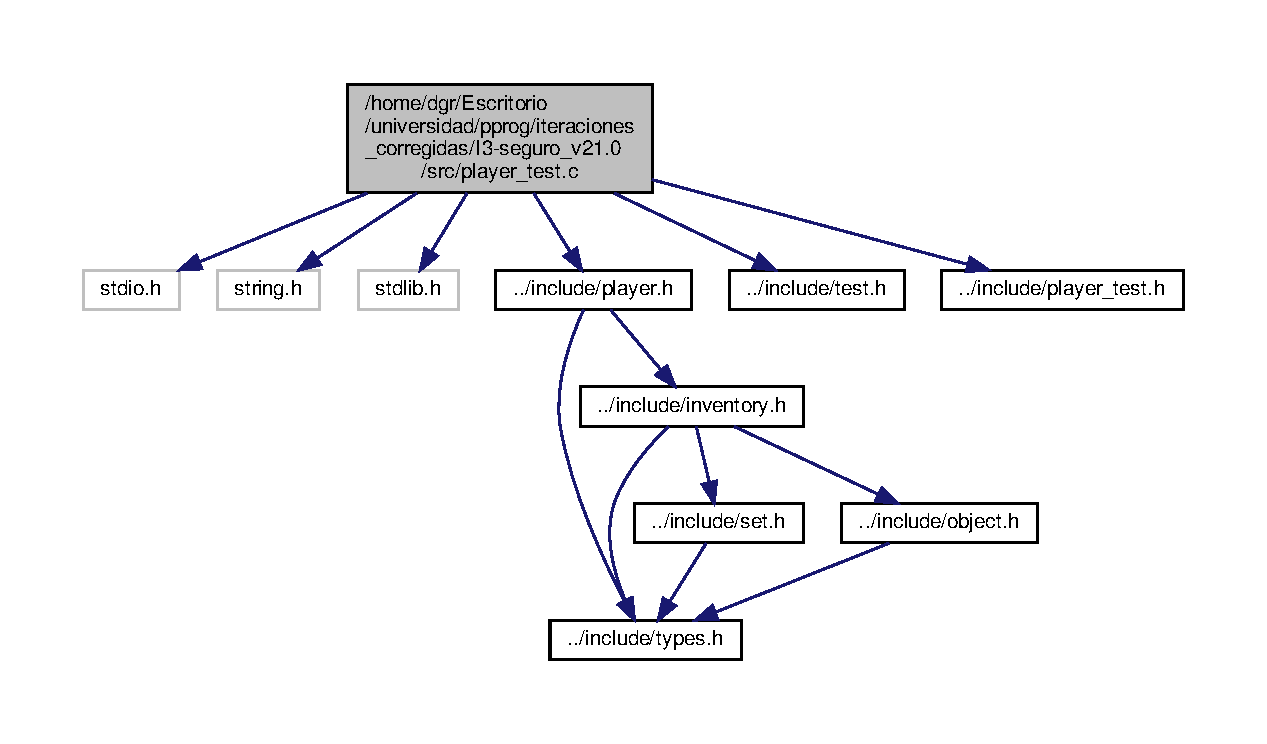
\includegraphics[width=350pt]{player__test_8c__incl}
\end{center}
\end{figure}
\subsection*{Macros}
\begin{DoxyCompactItemize}
\item 
\#define \hyperlink{player__test_8c_a2a77d2f2c5b698c69c19e1f8782bf709}{M\+A\+X\+\_\+\+T\+E\+S\+TS}~23
\begin{DoxyCompactList}\small\item\em maximum number of test \end{DoxyCompactList}\end{DoxyCompactItemize}
\subsection*{Functions}
\begin{DoxyCompactItemize}
\item 
int \hyperlink{player__test_8c_a3c04138a5bfe5d72780bb7e82a18e627}{main} (int argc, char $\ast$$\ast$argv)
\begin{DoxyCompactList}\small\item\em the main function of player\+\_\+test main \end{DoxyCompactList}\item 
void \hyperlink{player__test_8c_ab29768452373e16bb6aaa1f7998f62fb}{test1\+\_\+player\+\_\+create} ()
\item 
void \hyperlink{player__test_8c_a4f6eca5f9d8c08d2a7fc70c209ecf854}{test2\+\_\+player\+\_\+create} ()
\item 
void \hyperlink{player__test_8c_a14a3e4867e2ad3287c8efa99cd36904e}{test1\+\_\+player\+\_\+add\+\_\+object} ()
\item 
void \hyperlink{player__test_8c_a864d3935cf61953950b10df0e656306d}{test2\+\_\+player\+\_\+add\+\_\+object} ()
\item 
void \hyperlink{player__test_8c_ac984e5292c95002644a7af4fa499d0fb}{test3\+\_\+player\+\_\+add\+\_\+object} ()
\item 
void \hyperlink{player__test_8c_a5e2baa63ffa19a8676477e060ea784ca}{test1\+\_\+player\+\_\+dell\+\_\+object} ()
\item 
void \hyperlink{player__test_8c_a4a1855514d6fbd8387f730de40437cf4}{test2\+\_\+player\+\_\+dell\+\_\+object} ()
\item 
void \hyperlink{player__test_8c_aed6b8d0d4b733a8182faef777d6bb4d7}{test3\+\_\+player\+\_\+dell\+\_\+object} ()
\item 
void \hyperlink{player__test_8c_a27b5f30b6faa1d0bf8eb97fa9083a8e2}{test4\+\_\+player\+\_\+dell\+\_\+object} ()
\item 
void \hyperlink{player__test_8c_a9d87c09e6af910d695265e3fd77ae3a2}{test1\+\_\+player\+\_\+set\+\_\+name} ()
\item 
void \hyperlink{player__test_8c_a6e7ce8ff791f4bf63749df647a44263f}{test2\+\_\+player\+\_\+set\+\_\+name} ()
\item 
void \hyperlink{player__test_8c_a94068667d8faa66a4ad293dd2c60f2ef}{test1\+\_\+player\+\_\+get\+\_\+name} ()
\item 
void \hyperlink{player__test_8c_a3aa908fd360b74e7786422260e8e16a0}{test2\+\_\+player\+\_\+get\+\_\+name} ()
\item 
void \hyperlink{player__test_8c_aec6799a4f46c3f3c471fcb668addcad4}{test1\+\_\+player\+\_\+set\+\_\+location} ()
\item 
void \hyperlink{player__test_8c_a2c702753d9e2e3df9ef4abf2d1b9bc8d}{test2\+\_\+player\+\_\+set\+\_\+location} ()
\item 
void \hyperlink{player__test_8c_a408a557a0cff748c10fb9a03445af191}{test1\+\_\+player\+\_\+get\+\_\+location} ()
\item 
void \hyperlink{player__test_8c_a4c5605fac4bd716e1dfb2744db4fa8a1}{test2\+\_\+player\+\_\+get\+\_\+location} ()
\item 
void \hyperlink{player__test_8c_a64fa15a235953bea694236b9d7841cbc}{test1\+\_\+player\+\_\+set\+\_\+id} ()
\item 
void \hyperlink{player__test_8c_a3695e0896bc3d770290e6a691fa212f7}{test2\+\_\+player\+\_\+set\+\_\+id} ()
\item 
void \hyperlink{player__test_8c_a790a75dc179c00c60c784d3e34c0e5aa}{test1\+\_\+player\+\_\+get\+\_\+id} ()
\item 
void \hyperlink{player__test_8c_a9fa80f0c0e46b45eb9f1685b102a5826}{test2\+\_\+player\+\_\+get\+\_\+id} ()
\item 
void \hyperlink{player__test_8c_ad4a86b57bc18593265c205d7b27b9ecb}{test1\+\_\+player\+\_\+get\+\_\+inventory} ()
\item 
void \hyperlink{player__test_8c_a8f3a62c708fbed848568841ca8b1cd26}{test2\+\_\+player\+\_\+get\+\_\+inventory} ()
\end{DoxyCompactItemize}


\subsection{Detailed Description}
test to see if player works correctly 

\begin{DoxyAuthor}{Author}
Daniel Cerrato Sánchez 
\end{DoxyAuthor}
\begin{DoxyVersion}{Version}
2.\+0 
\end{DoxyVersion}
\begin{DoxyDate}{Date}
09-\/06-\/2020 
\end{DoxyDate}
\begin{DoxyCopyright}{Copyright}
G\+NU Public License 
\end{DoxyCopyright}


\subsection{Macro Definition Documentation}
\mbox{\Hypertarget{player__test_8c_a2a77d2f2c5b698c69c19e1f8782bf709}\label{player__test_8c_a2a77d2f2c5b698c69c19e1f8782bf709}} 
\index{player\+\_\+test.\+c@{player\+\_\+test.\+c}!M\+A\+X\+\_\+\+T\+E\+S\+TS@{M\+A\+X\+\_\+\+T\+E\+S\+TS}}
\index{M\+A\+X\+\_\+\+T\+E\+S\+TS@{M\+A\+X\+\_\+\+T\+E\+S\+TS}!player\+\_\+test.\+c@{player\+\_\+test.\+c}}
\subsubsection{\texorpdfstring{M\+A\+X\+\_\+\+T\+E\+S\+TS}{MAX\_TESTS}}
{\footnotesize\ttfamily \#define M\+A\+X\+\_\+\+T\+E\+S\+TS~23}



maximum number of test 

Details. 

\subsection{Function Documentation}
\mbox{\Hypertarget{player__test_8c_a3c04138a5bfe5d72780bb7e82a18e627}\label{player__test_8c_a3c04138a5bfe5d72780bb7e82a18e627}} 
\index{player\+\_\+test.\+c@{player\+\_\+test.\+c}!main@{main}}
\index{main@{main}!player\+\_\+test.\+c@{player\+\_\+test.\+c}}
\subsubsection{\texorpdfstring{main()}{main()}}
{\footnotesize\ttfamily int main (\begin{DoxyParamCaption}\item[{int}]{argc,  }\item[{char $\ast$$\ast$}]{argv }\end{DoxyParamCaption})}



the main function of player\+\_\+test main 

\begin{DoxyDate}{Date}
09-\/06-\/2020 
\end{DoxyDate}
\begin{DoxyAuthor}{Author}
Daniel Cerrato Sánchez 
\end{DoxyAuthor}
\begin{DoxyReturn}{Returns}

\end{DoxyReturn}
\mbox{\Hypertarget{player__test_8c_a14a3e4867e2ad3287c8efa99cd36904e}\label{player__test_8c_a14a3e4867e2ad3287c8efa99cd36904e}} 
\index{player\+\_\+test.\+c@{player\+\_\+test.\+c}!test1\+\_\+player\+\_\+add\+\_\+object@{test1\+\_\+player\+\_\+add\+\_\+object}}
\index{test1\+\_\+player\+\_\+add\+\_\+object@{test1\+\_\+player\+\_\+add\+\_\+object}!player\+\_\+test.\+c@{player\+\_\+test.\+c}}
\subsubsection{\texorpdfstring{test1\+\_\+player\+\_\+add\+\_\+object()}{test1\_player\_add\_object()}}
{\footnotesize\ttfamily void test1\+\_\+player\+\_\+add\+\_\+object (\begin{DoxyParamCaption}{ }\end{DoxyParamCaption})}

\begin{DoxyRefDesc}{Test}
\item[\hyperlink{test__test000201}{Test}]Test the function of adding an object to the player \end{DoxyRefDesc}
\begin{DoxyPrecond}{Precondition}
The player is a non-\/\+N\+U\+LL pointer, but the object is a N\+U\+LL pointer 
\end{DoxyPrecond}
\begin{DoxyPostcond}{Postcondition}
The output must be E\+R\+R\+OR 
\end{DoxyPostcond}
\mbox{\Hypertarget{player__test_8c_ab29768452373e16bb6aaa1f7998f62fb}\label{player__test_8c_ab29768452373e16bb6aaa1f7998f62fb}} 
\index{player\+\_\+test.\+c@{player\+\_\+test.\+c}!test1\+\_\+player\+\_\+create@{test1\+\_\+player\+\_\+create}}
\index{test1\+\_\+player\+\_\+create@{test1\+\_\+player\+\_\+create}!player\+\_\+test.\+c@{player\+\_\+test.\+c}}
\subsubsection{\texorpdfstring{test1\+\_\+player\+\_\+create()}{test1\_player\_create()}}
{\footnotesize\ttfamily void test1\+\_\+player\+\_\+create (\begin{DoxyParamCaption}{ }\end{DoxyParamCaption})}

\begin{DoxyRefDesc}{Test}
\item[\hyperlink{test__test000199}{Test}]Test the player creation function \end{DoxyRefDesc}
\begin{DoxyPrecond}{Precondition}
An id and an integer for the number of objects they can carry as parameters 
\end{DoxyPrecond}
\begin{DoxyPostcond}{Postcondition}
A non-\/null pointer to the created player 
\end{DoxyPostcond}
\mbox{\Hypertarget{player__test_8c_a5e2baa63ffa19a8676477e060ea784ca}\label{player__test_8c_a5e2baa63ffa19a8676477e060ea784ca}} 
\index{player\+\_\+test.\+c@{player\+\_\+test.\+c}!test1\+\_\+player\+\_\+dell\+\_\+object@{test1\+\_\+player\+\_\+dell\+\_\+object}}
\index{test1\+\_\+player\+\_\+dell\+\_\+object@{test1\+\_\+player\+\_\+dell\+\_\+object}!player\+\_\+test.\+c@{player\+\_\+test.\+c}}
\subsubsection{\texorpdfstring{test1\+\_\+player\+\_\+dell\+\_\+object()}{test1\_player\_dell\_object()}}
{\footnotesize\ttfamily void test1\+\_\+player\+\_\+dell\+\_\+object (\begin{DoxyParamCaption}{ }\end{DoxyParamCaption})}

\begin{DoxyRefDesc}{Test}
\item[\hyperlink{test__test000204}{Test}]Test the deletion function of a player object \end{DoxyRefDesc}
\begin{DoxyPrecond}{Precondition}
Player and object are non-\/\+N\+U\+LL pointers, correct object is searched 
\end{DoxyPrecond}
\begin{DoxyPostcond}{Postcondition}
The output must be OK 
\end{DoxyPostcond}
\mbox{\Hypertarget{player__test_8c_a790a75dc179c00c60c784d3e34c0e5aa}\label{player__test_8c_a790a75dc179c00c60c784d3e34c0e5aa}} 
\index{player\+\_\+test.\+c@{player\+\_\+test.\+c}!test1\+\_\+player\+\_\+get\+\_\+id@{test1\+\_\+player\+\_\+get\+\_\+id}}
\index{test1\+\_\+player\+\_\+get\+\_\+id@{test1\+\_\+player\+\_\+get\+\_\+id}!player\+\_\+test.\+c@{player\+\_\+test.\+c}}
\subsubsection{\texorpdfstring{test1\+\_\+player\+\_\+get\+\_\+id()}{test1\_player\_get\_id()}}
{\footnotesize\ttfamily void test1\+\_\+player\+\_\+get\+\_\+id (\begin{DoxyParamCaption}{ }\end{DoxyParamCaption})}

\begin{DoxyRefDesc}{Test}
\item[\hyperlink{test__test000218}{Test}]Test the function to get the id of a player \end{DoxyRefDesc}
\begin{DoxyPrecond}{Precondition}
The player is a non-\/\+N\+U\+LL pointer with a correct id 
\end{DoxyPrecond}
\begin{DoxyPostcond}{Postcondition}
The output must be OK 
\end{DoxyPostcond}
\mbox{\Hypertarget{player__test_8c_ad4a86b57bc18593265c205d7b27b9ecb}\label{player__test_8c_ad4a86b57bc18593265c205d7b27b9ecb}} 
\index{player\+\_\+test.\+c@{player\+\_\+test.\+c}!test1\+\_\+player\+\_\+get\+\_\+inventory@{test1\+\_\+player\+\_\+get\+\_\+inventory}}
\index{test1\+\_\+player\+\_\+get\+\_\+inventory@{test1\+\_\+player\+\_\+get\+\_\+inventory}!player\+\_\+test.\+c@{player\+\_\+test.\+c}}
\subsubsection{\texorpdfstring{test1\+\_\+player\+\_\+get\+\_\+inventory()}{test1\_player\_get\_inventory()}}
{\footnotesize\ttfamily void test1\+\_\+player\+\_\+get\+\_\+inventory (\begin{DoxyParamCaption}{ }\end{DoxyParamCaption})}

\begin{DoxyRefDesc}{Test}
\item[\hyperlink{test__test000220}{Test}]Test function to get player item set \end{DoxyRefDesc}
\begin{DoxyPrecond}{Precondition}
Player is a non-\/\+N\+U\+LL pointer with a correct set 
\end{DoxyPrecond}
\begin{DoxyPostcond}{Postcondition}
The output must be OK 
\end{DoxyPostcond}
\mbox{\Hypertarget{player__test_8c_a408a557a0cff748c10fb9a03445af191}\label{player__test_8c_a408a557a0cff748c10fb9a03445af191}} 
\index{player\+\_\+test.\+c@{player\+\_\+test.\+c}!test1\+\_\+player\+\_\+get\+\_\+location@{test1\+\_\+player\+\_\+get\+\_\+location}}
\index{test1\+\_\+player\+\_\+get\+\_\+location@{test1\+\_\+player\+\_\+get\+\_\+location}!player\+\_\+test.\+c@{player\+\_\+test.\+c}}
\subsubsection{\texorpdfstring{test1\+\_\+player\+\_\+get\+\_\+location()}{test1\_player\_get\_location()}}
{\footnotesize\ttfamily void test1\+\_\+player\+\_\+get\+\_\+location (\begin{DoxyParamCaption}{ }\end{DoxyParamCaption})}

\begin{DoxyRefDesc}{Test}
\item[\hyperlink{test__test000214}{Test}]Test the function to get the location of a player \end{DoxyRefDesc}
\begin{DoxyPrecond}{Precondition}
The player is a non-\/\+N\+U\+LL pointer in a correct space 
\end{DoxyPrecond}
\begin{DoxyPostcond}{Postcondition}
The output must be OK 
\end{DoxyPostcond}
\mbox{\Hypertarget{player__test_8c_a94068667d8faa66a4ad293dd2c60f2ef}\label{player__test_8c_a94068667d8faa66a4ad293dd2c60f2ef}} 
\index{player\+\_\+test.\+c@{player\+\_\+test.\+c}!test1\+\_\+player\+\_\+get\+\_\+name@{test1\+\_\+player\+\_\+get\+\_\+name}}
\index{test1\+\_\+player\+\_\+get\+\_\+name@{test1\+\_\+player\+\_\+get\+\_\+name}!player\+\_\+test.\+c@{player\+\_\+test.\+c}}
\subsubsection{\texorpdfstring{test1\+\_\+player\+\_\+get\+\_\+name()}{test1\_player\_get\_name()}}
{\footnotesize\ttfamily void test1\+\_\+player\+\_\+get\+\_\+name (\begin{DoxyParamCaption}{ }\end{DoxyParamCaption})}

\begin{DoxyRefDesc}{Test}
\item[\hyperlink{test__test000210}{Test}]Test function to get player name \end{DoxyRefDesc}
\begin{DoxyPrecond}{Precondition}
Player is a non-\/\+N\+U\+LL pointer with a correct name 
\end{DoxyPrecond}
\begin{DoxyPostcond}{Postcondition}
The comparison between the name and the word to compare must be 0 
\end{DoxyPostcond}
\mbox{\Hypertarget{player__test_8c_a64fa15a235953bea694236b9d7841cbc}\label{player__test_8c_a64fa15a235953bea694236b9d7841cbc}} 
\index{player\+\_\+test.\+c@{player\+\_\+test.\+c}!test1\+\_\+player\+\_\+set\+\_\+id@{test1\+\_\+player\+\_\+set\+\_\+id}}
\index{test1\+\_\+player\+\_\+set\+\_\+id@{test1\+\_\+player\+\_\+set\+\_\+id}!player\+\_\+test.\+c@{player\+\_\+test.\+c}}
\subsubsection{\texorpdfstring{test1\+\_\+player\+\_\+set\+\_\+id()}{test1\_player\_set\_id()}}
{\footnotesize\ttfamily void test1\+\_\+player\+\_\+set\+\_\+id (\begin{DoxyParamCaption}{ }\end{DoxyParamCaption})}

\begin{DoxyRefDesc}{Test}
\item[\hyperlink{test__test000216}{Test}]Test a player\textquotesingle{}s id change function \end{DoxyRefDesc}
\begin{DoxyPrecond}{Precondition}
The player is a non-\/\+N\+U\+LL pointer, the id is correct 
\end{DoxyPrecond}
\begin{DoxyPostcond}{Postcondition}
The output must be OK 
\end{DoxyPostcond}
\mbox{\Hypertarget{player__test_8c_aec6799a4f46c3f3c471fcb668addcad4}\label{player__test_8c_aec6799a4f46c3f3c471fcb668addcad4}} 
\index{player\+\_\+test.\+c@{player\+\_\+test.\+c}!test1\+\_\+player\+\_\+set\+\_\+location@{test1\+\_\+player\+\_\+set\+\_\+location}}
\index{test1\+\_\+player\+\_\+set\+\_\+location@{test1\+\_\+player\+\_\+set\+\_\+location}!player\+\_\+test.\+c@{player\+\_\+test.\+c}}
\subsubsection{\texorpdfstring{test1\+\_\+player\+\_\+set\+\_\+location()}{test1\_player\_set\_location()}}
{\footnotesize\ttfamily void test1\+\_\+player\+\_\+set\+\_\+location (\begin{DoxyParamCaption}{ }\end{DoxyParamCaption})}

\begin{DoxyRefDesc}{Test}
\item[\hyperlink{test__test000212}{Test}]Test a player\textquotesingle{}s location change function \end{DoxyRefDesc}
\begin{DoxyPrecond}{Precondition}
The player is a non-\/\+N\+U\+LL pointer, the space is correct 
\end{DoxyPrecond}
\begin{DoxyPostcond}{Postcondition}
The output must be OK 
\end{DoxyPostcond}
\mbox{\Hypertarget{player__test_8c_a9d87c09e6af910d695265e3fd77ae3a2}\label{player__test_8c_a9d87c09e6af910d695265e3fd77ae3a2}} 
\index{player\+\_\+test.\+c@{player\+\_\+test.\+c}!test1\+\_\+player\+\_\+set\+\_\+name@{test1\+\_\+player\+\_\+set\+\_\+name}}
\index{test1\+\_\+player\+\_\+set\+\_\+name@{test1\+\_\+player\+\_\+set\+\_\+name}!player\+\_\+test.\+c@{player\+\_\+test.\+c}}
\subsubsection{\texorpdfstring{test1\+\_\+player\+\_\+set\+\_\+name()}{test1\_player\_set\_name()}}
{\footnotesize\ttfamily void test1\+\_\+player\+\_\+set\+\_\+name (\begin{DoxyParamCaption}{ }\end{DoxyParamCaption})}

\begin{DoxyRefDesc}{Test}
\item[\hyperlink{test__test000208}{Test}]Test a player\textquotesingle{}s name change function \end{DoxyRefDesc}
\begin{DoxyPrecond}{Precondition}
The player is a non-\/\+N\+U\+LL pointer, the name is correct 
\end{DoxyPrecond}
\begin{DoxyPostcond}{Postcondition}
The output must be OK 
\end{DoxyPostcond}
\mbox{\Hypertarget{player__test_8c_a864d3935cf61953950b10df0e656306d}\label{player__test_8c_a864d3935cf61953950b10df0e656306d}} 
\index{player\+\_\+test.\+c@{player\+\_\+test.\+c}!test2\+\_\+player\+\_\+add\+\_\+object@{test2\+\_\+player\+\_\+add\+\_\+object}}
\index{test2\+\_\+player\+\_\+add\+\_\+object@{test2\+\_\+player\+\_\+add\+\_\+object}!player\+\_\+test.\+c@{player\+\_\+test.\+c}}
\subsubsection{\texorpdfstring{test2\+\_\+player\+\_\+add\+\_\+object()}{test2\_player\_add\_object()}}
{\footnotesize\ttfamily void test2\+\_\+player\+\_\+add\+\_\+object (\begin{DoxyParamCaption}{ }\end{DoxyParamCaption})}

\begin{DoxyRefDesc}{Test}
\item[\hyperlink{test__test000202}{Test}]Test the function of adding an object to the player \end{DoxyRefDesc}
\begin{DoxyPrecond}{Precondition}
The player is a non-\/\+N\+U\+LL pointer, the object is a N\+U\+LL pointer 
\end{DoxyPrecond}
\begin{DoxyPostcond}{Postcondition}
The output must be E\+R\+R\+OR 
\end{DoxyPostcond}
\mbox{\Hypertarget{player__test_8c_a4f6eca5f9d8c08d2a7fc70c209ecf854}\label{player__test_8c_a4f6eca5f9d8c08d2a7fc70c209ecf854}} 
\index{player\+\_\+test.\+c@{player\+\_\+test.\+c}!test2\+\_\+player\+\_\+create@{test2\+\_\+player\+\_\+create}}
\index{test2\+\_\+player\+\_\+create@{test2\+\_\+player\+\_\+create}!player\+\_\+test.\+c@{player\+\_\+test.\+c}}
\subsubsection{\texorpdfstring{test2\+\_\+player\+\_\+create()}{test2\_player\_create()}}
{\footnotesize\ttfamily void test2\+\_\+player\+\_\+create (\begin{DoxyParamCaption}{ }\end{DoxyParamCaption})}

\begin{DoxyRefDesc}{Test}
\item[\hyperlink{test__test000200}{Test}]Test the player creation function \end{DoxyRefDesc}
\begin{DoxyPrecond}{Precondition}
Player is a non-\/\+N\+U\+LL pointer 
\end{DoxyPrecond}
\begin{DoxyPostcond}{Postcondition}
The player id must be processed when creating it 
\end{DoxyPostcond}
\mbox{\Hypertarget{player__test_8c_a4a1855514d6fbd8387f730de40437cf4}\label{player__test_8c_a4a1855514d6fbd8387f730de40437cf4}} 
\index{player\+\_\+test.\+c@{player\+\_\+test.\+c}!test2\+\_\+player\+\_\+dell\+\_\+object@{test2\+\_\+player\+\_\+dell\+\_\+object}}
\index{test2\+\_\+player\+\_\+dell\+\_\+object@{test2\+\_\+player\+\_\+dell\+\_\+object}!player\+\_\+test.\+c@{player\+\_\+test.\+c}}
\subsubsection{\texorpdfstring{test2\+\_\+player\+\_\+dell\+\_\+object()}{test2\_player\_dell\_object()}}
{\footnotesize\ttfamily void test2\+\_\+player\+\_\+dell\+\_\+object (\begin{DoxyParamCaption}{ }\end{DoxyParamCaption})}

\begin{DoxyRefDesc}{Test}
\item[\hyperlink{test__test000205}{Test}]Test the deletion function of a player object \end{DoxyRefDesc}
\begin{DoxyPrecond}{Precondition}
Player and object are non-\/\+N\+U\+LL pointers, player has no object 
\end{DoxyPrecond}
\begin{DoxyPostcond}{Postcondition}
The output must be E\+R\+R\+OR 
\end{DoxyPostcond}
\mbox{\Hypertarget{player__test_8c_a9fa80f0c0e46b45eb9f1685b102a5826}\label{player__test_8c_a9fa80f0c0e46b45eb9f1685b102a5826}} 
\index{player\+\_\+test.\+c@{player\+\_\+test.\+c}!test2\+\_\+player\+\_\+get\+\_\+id@{test2\+\_\+player\+\_\+get\+\_\+id}}
\index{test2\+\_\+player\+\_\+get\+\_\+id@{test2\+\_\+player\+\_\+get\+\_\+id}!player\+\_\+test.\+c@{player\+\_\+test.\+c}}
\subsubsection{\texorpdfstring{test2\+\_\+player\+\_\+get\+\_\+id()}{test2\_player\_get\_id()}}
{\footnotesize\ttfamily void test2\+\_\+player\+\_\+get\+\_\+id (\begin{DoxyParamCaption}{ }\end{DoxyParamCaption})}

\begin{DoxyRefDesc}{Test}
\item[\hyperlink{test__test000219}{Test}]Test the function to get the id of a player \end{DoxyRefDesc}
\begin{DoxyPrecond}{Precondition}
Player is a pointer to N\+U\+LL 
\end{DoxyPrecond}
\begin{DoxyPostcond}{Postcondition}
The output must be E\+R\+R\+OR 
\end{DoxyPostcond}
\mbox{\Hypertarget{player__test_8c_a8f3a62c708fbed848568841ca8b1cd26}\label{player__test_8c_a8f3a62c708fbed848568841ca8b1cd26}} 
\index{player\+\_\+test.\+c@{player\+\_\+test.\+c}!test2\+\_\+player\+\_\+get\+\_\+inventory@{test2\+\_\+player\+\_\+get\+\_\+inventory}}
\index{test2\+\_\+player\+\_\+get\+\_\+inventory@{test2\+\_\+player\+\_\+get\+\_\+inventory}!player\+\_\+test.\+c@{player\+\_\+test.\+c}}
\subsubsection{\texorpdfstring{test2\+\_\+player\+\_\+get\+\_\+inventory()}{test2\_player\_get\_inventory()}}
{\footnotesize\ttfamily void test2\+\_\+player\+\_\+get\+\_\+inventory (\begin{DoxyParamCaption}{ }\end{DoxyParamCaption})}

\begin{DoxyRefDesc}{Test}
\item[\hyperlink{test__test000221}{Test}]Test function to get player item set \end{DoxyRefDesc}
\begin{DoxyPrecond}{Precondition}
Player is a pointer to N\+U\+LL 
\end{DoxyPrecond}
\begin{DoxyPostcond}{Postcondition}
The output must be E\+R\+R\+OR 
\end{DoxyPostcond}
\mbox{\Hypertarget{player__test_8c_a4c5605fac4bd716e1dfb2744db4fa8a1}\label{player__test_8c_a4c5605fac4bd716e1dfb2744db4fa8a1}} 
\index{player\+\_\+test.\+c@{player\+\_\+test.\+c}!test2\+\_\+player\+\_\+get\+\_\+location@{test2\+\_\+player\+\_\+get\+\_\+location}}
\index{test2\+\_\+player\+\_\+get\+\_\+location@{test2\+\_\+player\+\_\+get\+\_\+location}!player\+\_\+test.\+c@{player\+\_\+test.\+c}}
\subsubsection{\texorpdfstring{test2\+\_\+player\+\_\+get\+\_\+location()}{test2\_player\_get\_location()}}
{\footnotesize\ttfamily void test2\+\_\+player\+\_\+get\+\_\+location (\begin{DoxyParamCaption}{ }\end{DoxyParamCaption})}

\begin{DoxyRefDesc}{Test}
\item[\hyperlink{test__test000215}{Test}]Test the function to get the location of a player \end{DoxyRefDesc}
\begin{DoxyPrecond}{Precondition}
Player is a pointer to N\+U\+LL 
\end{DoxyPrecond}
\begin{DoxyPostcond}{Postcondition}
The output must be E\+R\+R\+OR 
\end{DoxyPostcond}
\mbox{\Hypertarget{player__test_8c_a3aa908fd360b74e7786422260e8e16a0}\label{player__test_8c_a3aa908fd360b74e7786422260e8e16a0}} 
\index{player\+\_\+test.\+c@{player\+\_\+test.\+c}!test2\+\_\+player\+\_\+get\+\_\+name@{test2\+\_\+player\+\_\+get\+\_\+name}}
\index{test2\+\_\+player\+\_\+get\+\_\+name@{test2\+\_\+player\+\_\+get\+\_\+name}!player\+\_\+test.\+c@{player\+\_\+test.\+c}}
\subsubsection{\texorpdfstring{test2\+\_\+player\+\_\+get\+\_\+name()}{test2\_player\_get\_name()}}
{\footnotesize\ttfamily void test2\+\_\+player\+\_\+get\+\_\+name (\begin{DoxyParamCaption}{ }\end{DoxyParamCaption})}

\begin{DoxyRefDesc}{Test}
\item[\hyperlink{test__test000211}{Test}]Test function to get player name \end{DoxyRefDesc}
\begin{DoxyPrecond}{Precondition}
Player is a pointer to N\+U\+LL 
\end{DoxyPrecond}
\begin{DoxyPostcond}{Postcondition}
The output must be E\+R\+R\+OR 
\end{DoxyPostcond}
\mbox{\Hypertarget{player__test_8c_a3695e0896bc3d770290e6a691fa212f7}\label{player__test_8c_a3695e0896bc3d770290e6a691fa212f7}} 
\index{player\+\_\+test.\+c@{player\+\_\+test.\+c}!test2\+\_\+player\+\_\+set\+\_\+id@{test2\+\_\+player\+\_\+set\+\_\+id}}
\index{test2\+\_\+player\+\_\+set\+\_\+id@{test2\+\_\+player\+\_\+set\+\_\+id}!player\+\_\+test.\+c@{player\+\_\+test.\+c}}
\subsubsection{\texorpdfstring{test2\+\_\+player\+\_\+set\+\_\+id()}{test2\_player\_set\_id()}}
{\footnotesize\ttfamily void test2\+\_\+player\+\_\+set\+\_\+id (\begin{DoxyParamCaption}{ }\end{DoxyParamCaption})}

\begin{DoxyRefDesc}{Test}
\item[\hyperlink{test__test000217}{Test}]Test a player\textquotesingle{}s id change function \end{DoxyRefDesc}
\begin{DoxyPrecond}{Precondition}
Player is a pointer to N\+U\+LL 
\end{DoxyPrecond}
\begin{DoxyPostcond}{Postcondition}
The output must be E\+R\+R\+OR 
\end{DoxyPostcond}
\mbox{\Hypertarget{player__test_8c_a2c702753d9e2e3df9ef4abf2d1b9bc8d}\label{player__test_8c_a2c702753d9e2e3df9ef4abf2d1b9bc8d}} 
\index{player\+\_\+test.\+c@{player\+\_\+test.\+c}!test2\+\_\+player\+\_\+set\+\_\+location@{test2\+\_\+player\+\_\+set\+\_\+location}}
\index{test2\+\_\+player\+\_\+set\+\_\+location@{test2\+\_\+player\+\_\+set\+\_\+location}!player\+\_\+test.\+c@{player\+\_\+test.\+c}}
\subsubsection{\texorpdfstring{test2\+\_\+player\+\_\+set\+\_\+location()}{test2\_player\_set\_location()}}
{\footnotesize\ttfamily void test2\+\_\+player\+\_\+set\+\_\+location (\begin{DoxyParamCaption}{ }\end{DoxyParamCaption})}

\begin{DoxyRefDesc}{Test}
\item[\hyperlink{test__test000213}{Test}]Test a player\textquotesingle{}s location change function \end{DoxyRefDesc}
\begin{DoxyPrecond}{Precondition}
Player is a pointer to N\+U\+LL 
\end{DoxyPrecond}
\begin{DoxyPostcond}{Postcondition}
The output must be E\+R\+R\+OR 
\end{DoxyPostcond}
\mbox{\Hypertarget{player__test_8c_a6e7ce8ff791f4bf63749df647a44263f}\label{player__test_8c_a6e7ce8ff791f4bf63749df647a44263f}} 
\index{player\+\_\+test.\+c@{player\+\_\+test.\+c}!test2\+\_\+player\+\_\+set\+\_\+name@{test2\+\_\+player\+\_\+set\+\_\+name}}
\index{test2\+\_\+player\+\_\+set\+\_\+name@{test2\+\_\+player\+\_\+set\+\_\+name}!player\+\_\+test.\+c@{player\+\_\+test.\+c}}
\subsubsection{\texorpdfstring{test2\+\_\+player\+\_\+set\+\_\+name()}{test2\_player\_set\_name()}}
{\footnotesize\ttfamily void test2\+\_\+player\+\_\+set\+\_\+name (\begin{DoxyParamCaption}{ }\end{DoxyParamCaption})}

\begin{DoxyRefDesc}{Test}
\item[\hyperlink{test__test000209}{Test}]Test a player\textquotesingle{}s name change function \end{DoxyRefDesc}
\begin{DoxyPrecond}{Precondition}
The player is a non-\/\+N\+U\+LL pointer, the name is N\+U\+LL 
\end{DoxyPrecond}
\begin{DoxyPostcond}{Postcondition}
The output must be E\+R\+R\+OR 
\end{DoxyPostcond}
\mbox{\Hypertarget{player__test_8c_ac984e5292c95002644a7af4fa499d0fb}\label{player__test_8c_ac984e5292c95002644a7af4fa499d0fb}} 
\index{player\+\_\+test.\+c@{player\+\_\+test.\+c}!test3\+\_\+player\+\_\+add\+\_\+object@{test3\+\_\+player\+\_\+add\+\_\+object}}
\index{test3\+\_\+player\+\_\+add\+\_\+object@{test3\+\_\+player\+\_\+add\+\_\+object}!player\+\_\+test.\+c@{player\+\_\+test.\+c}}
\subsubsection{\texorpdfstring{test3\+\_\+player\+\_\+add\+\_\+object()}{test3\_player\_add\_object()}}
{\footnotesize\ttfamily void test3\+\_\+player\+\_\+add\+\_\+object (\begin{DoxyParamCaption}{ }\end{DoxyParamCaption})}

\begin{DoxyRefDesc}{Test}
\item[\hyperlink{test__test000203}{Test}]Test the function of adding an object to the player \end{DoxyRefDesc}
\begin{DoxyPrecond}{Precondition}
Player is a N\+U\+LL pointer, object is a non-\/\+N\+U\+LL pointer 
\end{DoxyPrecond}
\begin{DoxyPostcond}{Postcondition}
The output must be E\+R\+R\+OR 
\end{DoxyPostcond}
\mbox{\Hypertarget{player__test_8c_aed6b8d0d4b733a8182faef777d6bb4d7}\label{player__test_8c_aed6b8d0d4b733a8182faef777d6bb4d7}} 
\index{player\+\_\+test.\+c@{player\+\_\+test.\+c}!test3\+\_\+player\+\_\+dell\+\_\+object@{test3\+\_\+player\+\_\+dell\+\_\+object}}
\index{test3\+\_\+player\+\_\+dell\+\_\+object@{test3\+\_\+player\+\_\+dell\+\_\+object}!player\+\_\+test.\+c@{player\+\_\+test.\+c}}
\subsubsection{\texorpdfstring{test3\+\_\+player\+\_\+dell\+\_\+object()}{test3\_player\_dell\_object()}}
{\footnotesize\ttfamily void test3\+\_\+player\+\_\+dell\+\_\+object (\begin{DoxyParamCaption}{ }\end{DoxyParamCaption})}

\begin{DoxyRefDesc}{Test}
\item[\hyperlink{test__test000206}{Test}]Test the deletion function of a player object \end{DoxyRefDesc}
\begin{DoxyPrecond}{Precondition}
Player and objects are non-\/\+N\+U\+LL pointers, wrong object is searched 
\end{DoxyPrecond}
\begin{DoxyPostcond}{Postcondition}
The output must be E\+R\+R\+OR 
\end{DoxyPostcond}
\mbox{\Hypertarget{player__test_8c_a27b5f30b6faa1d0bf8eb97fa9083a8e2}\label{player__test_8c_a27b5f30b6faa1d0bf8eb97fa9083a8e2}} 
\index{player\+\_\+test.\+c@{player\+\_\+test.\+c}!test4\+\_\+player\+\_\+dell\+\_\+object@{test4\+\_\+player\+\_\+dell\+\_\+object}}
\index{test4\+\_\+player\+\_\+dell\+\_\+object@{test4\+\_\+player\+\_\+dell\+\_\+object}!player\+\_\+test.\+c@{player\+\_\+test.\+c}}
\subsubsection{\texorpdfstring{test4\+\_\+player\+\_\+dell\+\_\+object()}{test4\_player\_dell\_object()}}
{\footnotesize\ttfamily void test4\+\_\+player\+\_\+dell\+\_\+object (\begin{DoxyParamCaption}{ }\end{DoxyParamCaption})}

\begin{DoxyRefDesc}{Test}
\item[\hyperlink{test__test000207}{Test}]Test the deletion function of a player object \end{DoxyRefDesc}
\begin{DoxyPrecond}{Precondition}
Player is a pointer to N\+U\+LL 
\end{DoxyPrecond}
\begin{DoxyPostcond}{Postcondition}
The output must be E\+R\+R\+OR 
\end{DoxyPostcond}

\hypertarget{screen_8c}{}\section{src/screen.c File Reference}
\label{screen_8c}\index{src/screen.\+c@{src/screen.\+c}}


is responsible for drawing the background of the game, also eliminates distractions from the thermianal, cleaning the screen  


{\ttfamily \#include $<$stdio.\+h$>$}\newline
{\ttfamily \#include $<$stdlib.\+h$>$}\newline
{\ttfamily \#include $<$string.\+h$>$}\newline
{\ttfamily \#include \char`\"{}../include/screen.\+h\char`\"{}}\newline
Include dependency graph for screen.\+c\+:\nopagebreak
\begin{figure}[H]
\begin{center}
\leavevmode
\includegraphics[width=350pt]{screen_8c__incl}
\end{center}
\end{figure}
\subsection*{Data Structures}
\begin{DoxyCompactItemize}
\item 
struct \hyperlink{struct__Area}{\+\_\+\+Area}
\begin{DoxyCompactList}\small\item\em The Area structure. \end{DoxyCompactList}\end{DoxyCompactItemize}
\subsection*{Macros}
\begin{DoxyCompactItemize}
\item 
\#define \hyperlink{screen_8c_a3cfd3aa62338d12609f6d65bce97e9cd}{R\+O\+WS}~35
\begin{DoxyCompactList}\small\item\em A macro that stores the number of rows. \end{DoxyCompactList}\item 
\#define \hyperlink{screen_8c_a06c6c391fc11d106e9909f0401b255b1}{C\+O\+L\+U\+M\+NS}~100
\begin{DoxyCompactList}\small\item\em A macro that stores the number of columns. \end{DoxyCompactList}\item 
\#define \hyperlink{screen_8c_afba5c5b9f73273ce653f890bb64740b0}{T\+O\+T\+A\+L\+\_\+\+D\+A\+TA}~(\hyperlink{screen_8c_a3cfd3aa62338d12609f6d65bce97e9cd}{R\+O\+WS} $\ast$ \hyperlink{screen_8c_a06c6c391fc11d106e9909f0401b255b1}{C\+O\+L\+U\+M\+NS}) + 1
\begin{DoxyCompactList}\small\item\em A macro that stores R\+O\+W\+S$\ast$\+C\+O\+L\+U\+M\+N\+S+1. \end{DoxyCompactList}\item 
\#define \hyperlink{screen_8c_a5e7c78a2c827b39d4464f2fc84058f87}{B\+G\+\_\+\+C\+H\+AR}~\textquotesingle{}$\sim$\textquotesingle{}
\begin{DoxyCompactList}\small\item\em B\+G\+\_\+\+C\+H\+AR. \end{DoxyCompactList}\item 
\#define \hyperlink{screen_8c_a0bbf43d51e6cd6f7119cf1d0063a3a94}{F\+G\+\_\+\+C\+H\+AR}~\textquotesingle{} \textquotesingle{}
\begin{DoxyCompactList}\small\item\em F\+G\+\_\+\+C\+H\+AR. \end{DoxyCompactList}\item 
\#define \hyperlink{screen_8c_accdbea14ea06c15e271784368bd993e8}{P\+R\+O\+M\+PT}~\char`\"{} prompt\+:$>$ \char`\"{}
\begin{DoxyCompactList}\small\item\em Prompt. \end{DoxyCompactList}\item 
\#define \hyperlink{screen_8c_a28b37557462b06fbb08e707dc0ba2136}{A\+C\+C\+E\+SS}(d,  x,  y)~(d + ((y)$\ast$\hyperlink{screen_8c_a06c6c391fc11d106e9909f0401b255b1}{C\+O\+L\+U\+M\+NS}) + (x))
\begin{DoxyCompactList}\small\item\em acces \end{DoxyCompactList}\end{DoxyCompactItemize}
\subsection*{Functions}
\begin{DoxyCompactItemize}
\item 
int \hyperlink{screen_8c_ad1b32d3d54fea228f1ef0c73de4a3929}{screen\+\_\+area\+\_\+cursor\+\_\+is\+\_\+out\+\_\+of\+\_\+bounds} (\hyperlink{screen_8h_acfdfc42f6522d75fa3c16713afde8127}{Area} $\ast$area)
\begin{DoxyCompactList}\small\item\em Prevents errors from occurring when the cursor is out of bounds. \end{DoxyCompactList}\item 
void \hyperlink{screen_8c_a110e0b378730322f5a2f1dc91e65e2aa}{screen\+\_\+area\+\_\+scroll\+\_\+up} (\hyperlink{screen_8h_acfdfc42f6522d75fa3c16713afde8127}{Area} $\ast$area)
\begin{DoxyCompactList}\small\item\em scroll up the area \end{DoxyCompactList}\item 
void \hyperlink{screen_8c_a55dedaa3b402fef825ceb6c3a957781d}{screen\+\_\+utils\+\_\+replaces\+\_\+special\+\_\+chars} (char $\ast$str)
\begin{DoxyCompactList}\small\item\em replace special chars \end{DoxyCompactList}\item 
void \hyperlink{screen_8c_a9dbb6c251337c03c078dc330caee48d2}{screen\+\_\+init} ()
\begin{DoxyCompactList}\small\item\em create the background \end{DoxyCompactList}\item 
void \hyperlink{screen_8c_a3d6d82dde2bb4f3ddc4d276dabe313ef}{screen\+\_\+destroy} ()
\begin{DoxyCompactList}\small\item\em free the screen \end{DoxyCompactList}\item 
void \hyperlink{screen_8c_a3eaa0547a956d39b6c55c9593524e0d1}{screen\+\_\+paint} ()
\begin{DoxyCompactList}\small\item\em print in the terminal the background with the data \end{DoxyCompactList}\item 
void \hyperlink{screen_8c_a57b2f852be623dca59255306c1482eb2}{screen\+\_\+gets} (char $\ast$str)
\begin{DoxyCompactList}\small\item\em get the information on the screen \end{DoxyCompactList}\item 
\hyperlink{screen_8h_acfdfc42f6522d75fa3c16713afde8127}{Area} $\ast$ \hyperlink{screen_8c_a194528bec3ed3b57618a8f2df9bea743}{screen\+\_\+area\+\_\+init} (int x, int y, int width, int height)
\begin{DoxyCompactList}\small\item\em create the area of the screen \end{DoxyCompactList}\item 
void \hyperlink{screen_8c_aca5123ed5a7afb75e79c0001e5d1df4f}{screen\+\_\+area\+\_\+destroy} (\hyperlink{screen_8h_acfdfc42f6522d75fa3c16713afde8127}{Area} $\ast$area)
\begin{DoxyCompactList}\small\item\em free the area of the screen \end{DoxyCompactList}\item 
void \hyperlink{screen_8c_a0950dc68cba3d491b909a8abaac1c666}{screen\+\_\+area\+\_\+clear} (\hyperlink{screen_8h_acfdfc42f6522d75fa3c16713afde8127}{Area} $\ast$area)
\begin{DoxyCompactList}\small\item\em clear the area \end{DoxyCompactList}\item 
void \hyperlink{screen_8c_af77fa9df4f7170e1e3bf1c6209b7f0c2}{screen\+\_\+area\+\_\+reset\+\_\+cursor} (\hyperlink{screen_8h_acfdfc42f6522d75fa3c16713afde8127}{Area} $\ast$area)
\begin{DoxyCompactList}\small\item\em reset the cursor \end{DoxyCompactList}\item 
void \hyperlink{screen_8c_a4f4cd4c7899c096d6c90cc33de9a9814}{screen\+\_\+area\+\_\+puts} (\hyperlink{screen_8h_acfdfc42f6522d75fa3c16713afde8127}{Area} $\ast$area, char $\ast$str)
\begin{DoxyCompactList}\small\item\em puts the area \end{DoxyCompactList}\end{DoxyCompactItemize}
\subsection*{Variables}
\begin{DoxyCompactItemize}
\item 
char $\ast$ \hyperlink{screen_8c_af05fac436b4ecde6c2a3f5af98124b51}{\+\_\+\+\_\+data}
\begin{DoxyCompactList}\small\item\em \+\_\+\+\_\+data \end{DoxyCompactList}\end{DoxyCompactItemize}


\subsection{Detailed Description}
is responsible for drawing the background of the game, also eliminates distractions from the thermianal, cleaning the screen 

\begin{DoxyAuthor}{Author}
Profesores P\+P\+R\+OG 
\end{DoxyAuthor}
\begin{DoxyVersion}{Version}
1.\+0 
\end{DoxyVersion}
\begin{DoxyDate}{Date}
13-\/01-\/2015 
\end{DoxyDate}
\begin{DoxyCopyright}{Copyright}
G\+NU Public License 
\end{DoxyCopyright}


\subsection{Macro Definition Documentation}
\mbox{\Hypertarget{screen_8c_a28b37557462b06fbb08e707dc0ba2136}\label{screen_8c_a28b37557462b06fbb08e707dc0ba2136}} 
\index{screen.\+c@{screen.\+c}!A\+C\+C\+E\+SS@{A\+C\+C\+E\+SS}}
\index{A\+C\+C\+E\+SS@{A\+C\+C\+E\+SS}!screen.\+c@{screen.\+c}}
\subsubsection{\texorpdfstring{A\+C\+C\+E\+SS}{ACCESS}}
{\footnotesize\ttfamily \#define A\+C\+C\+E\+SS(\begin{DoxyParamCaption}\item[{}]{d,  }\item[{}]{x,  }\item[{}]{y }\end{DoxyParamCaption})~(d + ((y)$\ast$\hyperlink{screen_8c_a06c6c391fc11d106e9909f0401b255b1}{C\+O\+L\+U\+M\+NS}) + (x))}



acces 

Details. \mbox{\Hypertarget{screen_8c_a5e7c78a2c827b39d4464f2fc84058f87}\label{screen_8c_a5e7c78a2c827b39d4464f2fc84058f87}} 
\index{screen.\+c@{screen.\+c}!B\+G\+\_\+\+C\+H\+AR@{B\+G\+\_\+\+C\+H\+AR}}
\index{B\+G\+\_\+\+C\+H\+AR@{B\+G\+\_\+\+C\+H\+AR}!screen.\+c@{screen.\+c}}
\subsubsection{\texorpdfstring{B\+G\+\_\+\+C\+H\+AR}{BG\_CHAR}}
{\footnotesize\ttfamily \#define B\+G\+\_\+\+C\+H\+AR~\textquotesingle{}$\sim$\textquotesingle{}}



B\+G\+\_\+\+C\+H\+AR. 

Details. \mbox{\Hypertarget{screen_8c_a06c6c391fc11d106e9909f0401b255b1}\label{screen_8c_a06c6c391fc11d106e9909f0401b255b1}} 
\index{screen.\+c@{screen.\+c}!C\+O\+L\+U\+M\+NS@{C\+O\+L\+U\+M\+NS}}
\index{C\+O\+L\+U\+M\+NS@{C\+O\+L\+U\+M\+NS}!screen.\+c@{screen.\+c}}
\subsubsection{\texorpdfstring{C\+O\+L\+U\+M\+NS}{COLUMNS}}
{\footnotesize\ttfamily \#define C\+O\+L\+U\+M\+NS~100}



A macro that stores the number of columns. 

Details. \mbox{\Hypertarget{screen_8c_a0bbf43d51e6cd6f7119cf1d0063a3a94}\label{screen_8c_a0bbf43d51e6cd6f7119cf1d0063a3a94}} 
\index{screen.\+c@{screen.\+c}!F\+G\+\_\+\+C\+H\+AR@{F\+G\+\_\+\+C\+H\+AR}}
\index{F\+G\+\_\+\+C\+H\+AR@{F\+G\+\_\+\+C\+H\+AR}!screen.\+c@{screen.\+c}}
\subsubsection{\texorpdfstring{F\+G\+\_\+\+C\+H\+AR}{FG\_CHAR}}
{\footnotesize\ttfamily \#define F\+G\+\_\+\+C\+H\+AR~\textquotesingle{} \textquotesingle{}}



F\+G\+\_\+\+C\+H\+AR. 

Details. \mbox{\Hypertarget{screen_8c_accdbea14ea06c15e271784368bd993e8}\label{screen_8c_accdbea14ea06c15e271784368bd993e8}} 
\index{screen.\+c@{screen.\+c}!P\+R\+O\+M\+PT@{P\+R\+O\+M\+PT}}
\index{P\+R\+O\+M\+PT@{P\+R\+O\+M\+PT}!screen.\+c@{screen.\+c}}
\subsubsection{\texorpdfstring{P\+R\+O\+M\+PT}{PROMPT}}
{\footnotesize\ttfamily \#define P\+R\+O\+M\+PT~\char`\"{} prompt\+:$>$ \char`\"{}}



Prompt. 

Details. \mbox{\Hypertarget{screen_8c_a3cfd3aa62338d12609f6d65bce97e9cd}\label{screen_8c_a3cfd3aa62338d12609f6d65bce97e9cd}} 
\index{screen.\+c@{screen.\+c}!R\+O\+WS@{R\+O\+WS}}
\index{R\+O\+WS@{R\+O\+WS}!screen.\+c@{screen.\+c}}
\subsubsection{\texorpdfstring{R\+O\+WS}{ROWS}}
{\footnotesize\ttfamily \#define R\+O\+WS~35}



A macro that stores the number of rows. 

Details. \mbox{\Hypertarget{screen_8c_afba5c5b9f73273ce653f890bb64740b0}\label{screen_8c_afba5c5b9f73273ce653f890bb64740b0}} 
\index{screen.\+c@{screen.\+c}!T\+O\+T\+A\+L\+\_\+\+D\+A\+TA@{T\+O\+T\+A\+L\+\_\+\+D\+A\+TA}}
\index{T\+O\+T\+A\+L\+\_\+\+D\+A\+TA@{T\+O\+T\+A\+L\+\_\+\+D\+A\+TA}!screen.\+c@{screen.\+c}}
\subsubsection{\texorpdfstring{T\+O\+T\+A\+L\+\_\+\+D\+A\+TA}{TOTAL\_DATA}}
{\footnotesize\ttfamily \#define T\+O\+T\+A\+L\+\_\+\+D\+A\+TA~(\hyperlink{screen_8c_a3cfd3aa62338d12609f6d65bce97e9cd}{R\+O\+WS} $\ast$ \hyperlink{screen_8c_a06c6c391fc11d106e9909f0401b255b1}{C\+O\+L\+U\+M\+NS}) + 1}



A macro that stores R\+O\+W\+S$\ast$\+C\+O\+L\+U\+M\+N\+S+1. 

Details. 

\subsection{Function Documentation}
\mbox{\Hypertarget{screen_8c_a0950dc68cba3d491b909a8abaac1c666}\label{screen_8c_a0950dc68cba3d491b909a8abaac1c666}} 
\index{screen.\+c@{screen.\+c}!screen\+\_\+area\+\_\+clear@{screen\+\_\+area\+\_\+clear}}
\index{screen\+\_\+area\+\_\+clear@{screen\+\_\+area\+\_\+clear}!screen.\+c@{screen.\+c}}
\subsubsection{\texorpdfstring{screen\+\_\+area\+\_\+clear()}{screen\_area\_clear()}}
{\footnotesize\ttfamily void screen\+\_\+area\+\_\+clear (\begin{DoxyParamCaption}\item[{\hyperlink{screen_8h_acfdfc42f6522d75fa3c16713afde8127}{Area} $\ast$}]{area }\end{DoxyParamCaption})}



clear the area 

screen\+\_\+area\+\_\+clear

\begin{DoxyDate}{Date}
13-\/01-\/2015 
\end{DoxyDate}
\begin{DoxyAuthor}{Author}
\+: Instructors of P\+P\+R\+OG
\end{DoxyAuthor}
param area the area we want to modified \mbox{\Hypertarget{screen_8c_ad1b32d3d54fea228f1ef0c73de4a3929}\label{screen_8c_ad1b32d3d54fea228f1ef0c73de4a3929}} 
\index{screen.\+c@{screen.\+c}!screen\+\_\+area\+\_\+cursor\+\_\+is\+\_\+out\+\_\+of\+\_\+bounds@{screen\+\_\+area\+\_\+cursor\+\_\+is\+\_\+out\+\_\+of\+\_\+bounds}}
\index{screen\+\_\+area\+\_\+cursor\+\_\+is\+\_\+out\+\_\+of\+\_\+bounds@{screen\+\_\+area\+\_\+cursor\+\_\+is\+\_\+out\+\_\+of\+\_\+bounds}!screen.\+c@{screen.\+c}}
\subsubsection{\texorpdfstring{screen\+\_\+area\+\_\+cursor\+\_\+is\+\_\+out\+\_\+of\+\_\+bounds()}{screen\_area\_cursor\_is\_out\_of\_bounds()}}
{\footnotesize\ttfamily int screen\+\_\+area\+\_\+cursor\+\_\+is\+\_\+out\+\_\+of\+\_\+bounds (\begin{DoxyParamCaption}\item[{\hyperlink{screen_8h_acfdfc42f6522d75fa3c16713afde8127}{Area} $\ast$}]{area }\end{DoxyParamCaption})}



Prevents errors from occurring when the cursor is out of bounds. 

screen\+\_\+area\+\_\+cursor\+\_\+is\+\_\+out\+\_\+of\+\_\+bounds

\begin{DoxyDate}{Date}
13-\/01-\/2015 
\end{DoxyDate}
\begin{DoxyAuthor}{Author}
\+: Instructors of P\+P\+R\+OG
\end{DoxyAuthor}
param area the area we want to modified return area-\/$>$cursor the cursor we have modified \mbox{\Hypertarget{screen_8c_aca5123ed5a7afb75e79c0001e5d1df4f}\label{screen_8c_aca5123ed5a7afb75e79c0001e5d1df4f}} 
\index{screen.\+c@{screen.\+c}!screen\+\_\+area\+\_\+destroy@{screen\+\_\+area\+\_\+destroy}}
\index{screen\+\_\+area\+\_\+destroy@{screen\+\_\+area\+\_\+destroy}!screen.\+c@{screen.\+c}}
\subsubsection{\texorpdfstring{screen\+\_\+area\+\_\+destroy()}{screen\_area\_destroy()}}
{\footnotesize\ttfamily void screen\+\_\+area\+\_\+destroy (\begin{DoxyParamCaption}\item[{\hyperlink{screen_8h_acfdfc42f6522d75fa3c16713afde8127}{Area} $\ast$}]{area }\end{DoxyParamCaption})}



free the area of the screen 

screen\+\_\+destroy free a especific space

\begin{DoxyDate}{Date}
13-\/01-\/2015 
\end{DoxyDate}
\begin{DoxyAuthor}{Author}
\+: Instructors of P\+P\+R\+OG
\end{DoxyAuthor}
param area the area we want free \mbox{\Hypertarget{screen_8c_a194528bec3ed3b57618a8f2df9bea743}\label{screen_8c_a194528bec3ed3b57618a8f2df9bea743}} 
\index{screen.\+c@{screen.\+c}!screen\+\_\+area\+\_\+init@{screen\+\_\+area\+\_\+init}}
\index{screen\+\_\+area\+\_\+init@{screen\+\_\+area\+\_\+init}!screen.\+c@{screen.\+c}}
\subsubsection{\texorpdfstring{screen\+\_\+area\+\_\+init()}{screen\_area\_init()}}
{\footnotesize\ttfamily \hyperlink{screen_8h_acfdfc42f6522d75fa3c16713afde8127}{Area}$\ast$ screen\+\_\+area\+\_\+init (\begin{DoxyParamCaption}\item[{int}]{x,  }\item[{int}]{y,  }\item[{int}]{width,  }\item[{int}]{height }\end{DoxyParamCaption})}



create the area of the screen 

screen\+\_\+area\+\_\+init

\begin{DoxyDate}{Date}
13-\/01-\/2015 
\end{DoxyDate}
\begin{DoxyAuthor}{Author}
\+: Instructors of P\+P\+R\+OG
\end{DoxyAuthor}

\begin{DoxyParams}{Parameters}
{\em x} & coordinate x \\
\hline
{\em y} & coordinate y \\
\hline
{\em width} & coordinate width \\
\hline
{\em height} & coordinate height \\
\hline
\end{DoxyParams}
\begin{DoxyReturn}{Returns}
area the area that has been created 
\end{DoxyReturn}
\mbox{\Hypertarget{screen_8c_a4f4cd4c7899c096d6c90cc33de9a9814}\label{screen_8c_a4f4cd4c7899c096d6c90cc33de9a9814}} 
\index{screen.\+c@{screen.\+c}!screen\+\_\+area\+\_\+puts@{screen\+\_\+area\+\_\+puts}}
\index{screen\+\_\+area\+\_\+puts@{screen\+\_\+area\+\_\+puts}!screen.\+c@{screen.\+c}}
\subsubsection{\texorpdfstring{screen\+\_\+area\+\_\+puts()}{screen\_area\_puts()}}
{\footnotesize\ttfamily void screen\+\_\+area\+\_\+puts (\begin{DoxyParamCaption}\item[{\hyperlink{screen_8h_acfdfc42f6522d75fa3c16713afde8127}{Area} $\ast$}]{area,  }\item[{char $\ast$}]{str }\end{DoxyParamCaption})}



puts the area 

screen\+\_\+area\+\_\+puts

\begin{DoxyDate}{Date}
13-\/01-\/2015 
\end{DoxyDate}
\begin{DoxyAuthor}{Author}
\+: Instructors of P\+P\+R\+OG
\end{DoxyAuthor}
param area the area we want to modified param str the string we will use \mbox{\Hypertarget{screen_8c_af77fa9df4f7170e1e3bf1c6209b7f0c2}\label{screen_8c_af77fa9df4f7170e1e3bf1c6209b7f0c2}} 
\index{screen.\+c@{screen.\+c}!screen\+\_\+area\+\_\+reset\+\_\+cursor@{screen\+\_\+area\+\_\+reset\+\_\+cursor}}
\index{screen\+\_\+area\+\_\+reset\+\_\+cursor@{screen\+\_\+area\+\_\+reset\+\_\+cursor}!screen.\+c@{screen.\+c}}
\subsubsection{\texorpdfstring{screen\+\_\+area\+\_\+reset\+\_\+cursor()}{screen\_area\_reset\_cursor()}}
{\footnotesize\ttfamily void screen\+\_\+area\+\_\+reset\+\_\+cursor (\begin{DoxyParamCaption}\item[{\hyperlink{screen_8h_acfdfc42f6522d75fa3c16713afde8127}{Area} $\ast$}]{area }\end{DoxyParamCaption})}



reset the cursor 

screen\+\_\+area\+\_\+reset\+\_\+cursor

\begin{DoxyDate}{Date}
13-\/01-\/2015 
\end{DoxyDate}
\begin{DoxyAuthor}{Author}
\+: Instructors of P\+P\+R\+OG
\end{DoxyAuthor}
param area the area we want to modified \mbox{\Hypertarget{screen_8c_a110e0b378730322f5a2f1dc91e65e2aa}\label{screen_8c_a110e0b378730322f5a2f1dc91e65e2aa}} 
\index{screen.\+c@{screen.\+c}!screen\+\_\+area\+\_\+scroll\+\_\+up@{screen\+\_\+area\+\_\+scroll\+\_\+up}}
\index{screen\+\_\+area\+\_\+scroll\+\_\+up@{screen\+\_\+area\+\_\+scroll\+\_\+up}!screen.\+c@{screen.\+c}}
\subsubsection{\texorpdfstring{screen\+\_\+area\+\_\+scroll\+\_\+up()}{screen\_area\_scroll\_up()}}
{\footnotesize\ttfamily void screen\+\_\+area\+\_\+scroll\+\_\+up (\begin{DoxyParamCaption}\item[{\hyperlink{screen_8h_acfdfc42f6522d75fa3c16713afde8127}{Area} $\ast$}]{area }\end{DoxyParamCaption})}



scroll up the area 

screen\+\_\+area\+\_\+scroll\+\_\+up

\begin{DoxyDate}{Date}
13-\/01-\/2015 
\end{DoxyDate}
\begin{DoxyAuthor}{Author}
\+: Instructors of P\+P\+R\+OG
\end{DoxyAuthor}
param area the area we want to modified \mbox{\Hypertarget{screen_8c_a3d6d82dde2bb4f3ddc4d276dabe313ef}\label{screen_8c_a3d6d82dde2bb4f3ddc4d276dabe313ef}} 
\index{screen.\+c@{screen.\+c}!screen\+\_\+destroy@{screen\+\_\+destroy}}
\index{screen\+\_\+destroy@{screen\+\_\+destroy}!screen.\+c@{screen.\+c}}
\subsubsection{\texorpdfstring{screen\+\_\+destroy()}{screen\_destroy()}}
{\footnotesize\ttfamily void screen\+\_\+destroy (\begin{DoxyParamCaption}{ }\end{DoxyParamCaption})}



free the screen 

screen\+\_\+destroy free a especific space

\begin{DoxyDate}{Date}
13-\/01-\/2015 
\end{DoxyDate}
\begin{DoxyAuthor}{Author}
\+: Instructors of P\+P\+R\+OG 
\end{DoxyAuthor}
\mbox{\Hypertarget{screen_8c_a57b2f852be623dca59255306c1482eb2}\label{screen_8c_a57b2f852be623dca59255306c1482eb2}} 
\index{screen.\+c@{screen.\+c}!screen\+\_\+gets@{screen\+\_\+gets}}
\index{screen\+\_\+gets@{screen\+\_\+gets}!screen.\+c@{screen.\+c}}
\subsubsection{\texorpdfstring{screen\+\_\+gets()}{screen\_gets()}}
{\footnotesize\ttfamily void screen\+\_\+gets (\begin{DoxyParamCaption}\item[{char $\ast$}]{str }\end{DoxyParamCaption})}



get the information on the screen 

screen\+\_\+gets

\begin{DoxyDate}{Date}
13-\/01-\/2015 
\end{DoxyDate}
\begin{DoxyAuthor}{Author}
\+: Instructors of P\+P\+R\+OG 
\end{DoxyAuthor}
\mbox{\Hypertarget{screen_8c_a9dbb6c251337c03c078dc330caee48d2}\label{screen_8c_a9dbb6c251337c03c078dc330caee48d2}} 
\index{screen.\+c@{screen.\+c}!screen\+\_\+init@{screen\+\_\+init}}
\index{screen\+\_\+init@{screen\+\_\+init}!screen.\+c@{screen.\+c}}
\subsubsection{\texorpdfstring{screen\+\_\+init()}{screen\_init()}}
{\footnotesize\ttfamily void screen\+\_\+init (\begin{DoxyParamCaption}{ }\end{DoxyParamCaption})}



create the background 

screen\+\_\+init

\begin{DoxyDate}{Date}
13-\/01-\/2015 
\end{DoxyDate}
\begin{DoxyAuthor}{Author}
\+: Instructors of P\+P\+R\+OG 
\end{DoxyAuthor}
\mbox{\Hypertarget{screen_8c_a3eaa0547a956d39b6c55c9593524e0d1}\label{screen_8c_a3eaa0547a956d39b6c55c9593524e0d1}} 
\index{screen.\+c@{screen.\+c}!screen\+\_\+paint@{screen\+\_\+paint}}
\index{screen\+\_\+paint@{screen\+\_\+paint}!screen.\+c@{screen.\+c}}
\subsubsection{\texorpdfstring{screen\+\_\+paint()}{screen\_paint()}}
{\footnotesize\ttfamily void screen\+\_\+paint (\begin{DoxyParamCaption}{ }\end{DoxyParamCaption})}



print in the terminal the background with the data 

screen\+\_\+paint

\begin{DoxyDate}{Date}
13-\/01-\/2015 
\end{DoxyDate}
\begin{DoxyAuthor}{Author}
\+: Instructors of P\+P\+R\+OG 
\end{DoxyAuthor}
\mbox{\Hypertarget{screen_8c_a55dedaa3b402fef825ceb6c3a957781d}\label{screen_8c_a55dedaa3b402fef825ceb6c3a957781d}} 
\index{screen.\+c@{screen.\+c}!screen\+\_\+utils\+\_\+replaces\+\_\+special\+\_\+chars@{screen\+\_\+utils\+\_\+replaces\+\_\+special\+\_\+chars}}
\index{screen\+\_\+utils\+\_\+replaces\+\_\+special\+\_\+chars@{screen\+\_\+utils\+\_\+replaces\+\_\+special\+\_\+chars}!screen.\+c@{screen.\+c}}
\subsubsection{\texorpdfstring{screen\+\_\+utils\+\_\+replaces\+\_\+special\+\_\+chars()}{screen\_utils\_replaces\_special\_chars()}}
{\footnotesize\ttfamily void screen\+\_\+utils\+\_\+replaces\+\_\+special\+\_\+chars (\begin{DoxyParamCaption}\item[{char $\ast$}]{str }\end{DoxyParamCaption})}



replace special chars 

screen\+\_\+utils\+\_\+replaces\+\_\+special\+\_\+chars

\begin{DoxyDate}{Date}
13-\/01-\/2015 
\end{DoxyDate}
\begin{DoxyAuthor}{Author}
\+: Instructors of P\+P\+R\+OG
\end{DoxyAuthor}
param str the string with the special characters 

\subsection{Variable Documentation}
\mbox{\Hypertarget{screen_8c_af05fac436b4ecde6c2a3f5af98124b51}\label{screen_8c_af05fac436b4ecde6c2a3f5af98124b51}} 
\index{screen.\+c@{screen.\+c}!\+\_\+\+\_\+data@{\+\_\+\+\_\+data}}
\index{\+\_\+\+\_\+data@{\+\_\+\+\_\+data}!screen.\+c@{screen.\+c}}
\subsubsection{\texorpdfstring{\+\_\+\+\_\+data}{\_\_data}}
{\footnotesize\ttfamily \+\_\+\+\_\+data}



\+\_\+\+\_\+data 

Details. 
\hypertarget{set_8c}{}\section{src/set.c File Reference}
\label{set_8c}\index{src/set.\+c@{src/set.\+c}}


It implements the set interface.  


{\ttfamily \#include $<$stdio.\+h$>$}\newline
{\ttfamily \#include $<$stdlib.\+h$>$}\newline
{\ttfamily \#include \char`\"{}../include/types.\+h\char`\"{}}\newline
{\ttfamily \#include \char`\"{}../include/set.\+h\char`\"{}}\newline
Include dependency graph for set.\+c\+:\nopagebreak
\begin{figure}[H]
\begin{center}
\leavevmode
\includegraphics[width=279pt]{set_8c__incl}
\end{center}
\end{figure}
\subsection*{Data Structures}
\begin{DoxyCompactItemize}
\item 
struct \hyperlink{struct__Set}{\+\_\+\+Set}
\begin{DoxyCompactList}\small\item\em The set structure. \end{DoxyCompactList}\end{DoxyCompactItemize}
\subsection*{Macros}
\begin{DoxyCompactItemize}
\item 
\#define \hyperlink{set_8c_a1cdef4472847c938fc165b7d2737c4e4}{M\+A\+X\+\_\+\+ID}~50
\begin{DoxyCompactList}\small\item\em maimum number of id of the set \end{DoxyCompactList}\end{DoxyCompactItemize}
\subsection*{Functions}
\begin{DoxyCompactItemize}
\item 
\hyperlink{set_8h_a6d3b7f7c92cbb4577ef3ef7ddbf93161}{Set} $\ast$ \hyperlink{set_8c_abcc73b7ad3913fc92dd95d366c9c8687}{set\+\_\+create} ()
\begin{DoxyCompactList}\small\item\em Create the set. \end{DoxyCompactList}\item 
\hyperlink{types_8h_a32c27cc471df37f4fc818d65de0a56c4}{S\+T\+A\+T\+US} \hyperlink{set_8c_a17fa263a49d6fe209c040e9ca5e0132a}{set\+\_\+destroy} (\hyperlink{set_8h_a6d3b7f7c92cbb4577ef3ef7ddbf93161}{Set} $\ast$set)
\begin{DoxyCompactList}\small\item\em Destroy the set. \end{DoxyCompactList}\item 
\hyperlink{types_8h_a32c27cc471df37f4fc818d65de0a56c4}{S\+T\+A\+T\+US} \hyperlink{set_8c_a214235069ee276ad9bceb2c66e56bfe1}{set\+\_\+add} (\hyperlink{set_8h_a6d3b7f7c92cbb4577ef3ef7ddbf93161}{Set} $\ast$set, \hyperlink{types_8h_a845e604fb28f7e3d97549da3448149d3}{Id} id)
\begin{DoxyCompactList}\small\item\em Add element to the set. \end{DoxyCompactList}\item 
\hyperlink{types_8h_a32c27cc471df37f4fc818d65de0a56c4}{S\+T\+A\+T\+US} \hyperlink{set_8c_a7132be7ebdf9b2d3b1f23895a59a25df}{set\+\_\+dell} (\hyperlink{set_8h_a6d3b7f7c92cbb4577ef3ef7ddbf93161}{Set} $\ast$set, \hyperlink{types_8h_a845e604fb28f7e3d97549da3448149d3}{Id} id)
\begin{DoxyCompactList}\small\item\em remove or delete an id in a set \end{DoxyCompactList}\item 
int \hyperlink{set_8c_a62a3c1e0de34be5b9b2f5161a430f090}{set\+\_\+get\+\_\+num} (\hyperlink{set_8h_a6d3b7f7c92cbb4577ef3ef7ddbf93161}{Set} $\ast$set)
\begin{DoxyCompactList}\small\item\em return the namber of id allocated in a set \end{DoxyCompactList}\item 
int \hyperlink{set_8c_a565a873b0d50133d4c48319e8b6b13d9}{set\+\_\+find\+\_\+index} (\hyperlink{set_8h_a6d3b7f7c92cbb4577ef3ef7ddbf93161}{Set} $\ast$set, \hyperlink{types_8h_a845e604fb28f7e3d97549da3448149d3}{Id} id)
\begin{DoxyCompactList}\small\item\em return the index of and id \end{DoxyCompactList}\item 
\hyperlink{types_8h_a845e604fb28f7e3d97549da3448149d3}{Id} \hyperlink{set_8c_a37b5d27dabd419279fe1eddc40cec0fa}{set\+\_\+get\+\_\+id\+\_\+at\+\_\+position} (\hyperlink{set_8h_a6d3b7f7c92cbb4577ef3ef7ddbf93161}{Set} $\ast$set, int position)
\begin{DoxyCompactList}\small\item\em returns the id of the indicated position \end{DoxyCompactList}\item 
void \hyperlink{set_8c_ab7cd9162335d346f5457eef63692a96b}{set\+\_\+print} (F\+I\+LE $\ast$f, \hyperlink{set_8h_a6d3b7f7c92cbb4577ef3ef7ddbf93161}{Set} $\ast$set)
\begin{DoxyCompactList}\small\item\em print the elements of the set \end{DoxyCompactList}\item 
\hyperlink{types_8h_a32c27cc471df37f4fc818d65de0a56c4}{S\+T\+A\+T\+US} \hyperlink{set_8c_ac996936009c685a89fdc26c27a9b1874}{set\+\_\+update} (\hyperlink{set_8h_a6d3b7f7c92cbb4577ef3ef7ddbf93161}{Set} $\ast$original, \hyperlink{set_8h_a6d3b7f7c92cbb4577ef3ef7ddbf93161}{Set} $\ast$final)
\begin{DoxyCompactList}\small\item\em update a set with a new set \end{DoxyCompactList}\end{DoxyCompactItemize}


\subsection{Detailed Description}
It implements the set interface. 

\begin{DoxyAuthor}{Author}

\end{DoxyAuthor}
\begin{DoxyVersion}{Version}
1.\+0 
\end{DoxyVersion}
\begin{DoxyDate}{Date}
18-\/02-\/2020 
\end{DoxyDate}
\begin{DoxyCopyright}{Copyright}
G\+NU Public License 
\end{DoxyCopyright}


\subsection{Macro Definition Documentation}
\mbox{\Hypertarget{set_8c_a1cdef4472847c938fc165b7d2737c4e4}\label{set_8c_a1cdef4472847c938fc165b7d2737c4e4}} 
\index{set.\+c@{set.\+c}!M\+A\+X\+\_\+\+ID@{M\+A\+X\+\_\+\+ID}}
\index{M\+A\+X\+\_\+\+ID@{M\+A\+X\+\_\+\+ID}!set.\+c@{set.\+c}}
\subsubsection{\texorpdfstring{M\+A\+X\+\_\+\+ID}{MAX\_ID}}
{\footnotesize\ttfamily \#define M\+A\+X\+\_\+\+ID~50}



maimum number of id of the set 

Details. 

\subsection{Function Documentation}
\mbox{\Hypertarget{set_8c_a214235069ee276ad9bceb2c66e56bfe1}\label{set_8c_a214235069ee276ad9bceb2c66e56bfe1}} 
\index{set.\+c@{set.\+c}!set\+\_\+add@{set\+\_\+add}}
\index{set\+\_\+add@{set\+\_\+add}!set.\+c@{set.\+c}}
\subsubsection{\texorpdfstring{set\+\_\+add()}{set\_add()}}
{\footnotesize\ttfamily \hyperlink{types_8h_a32c27cc471df37f4fc818d65de0a56c4}{S\+T\+A\+T\+US} set\+\_\+add (\begin{DoxyParamCaption}\item[{\hyperlink{set_8h_a6d3b7f7c92cbb4577ef3ef7ddbf93161}{Set} $\ast$}]{set,  }\item[{\hyperlink{types_8h_a845e604fb28f7e3d97549da3448149d3}{Id}}]{id }\end{DoxyParamCaption})}



Add element to the set. 

set\+\_\+add add an element to the set

\begin{DoxyDate}{Date}
20-\/02-\/2020 
\end{DoxyDate}
\begin{DoxyAuthor}{Author}
David Teófilo Garitagoitia Romero
\end{DoxyAuthor}

\begin{DoxyParams}{Parameters}
{\em set} & the addres os the set in which you want to add an element \\
\hline
{\em id} & the id of the element that you want to add \\
\hline
\end{DoxyParams}
\begin{DoxyReturn}{Returns}
Ok if there was no problem, 
\end{DoxyReturn}
\mbox{\Hypertarget{set_8c_abcc73b7ad3913fc92dd95d366c9c8687}\label{set_8c_abcc73b7ad3913fc92dd95d366c9c8687}} 
\index{set.\+c@{set.\+c}!set\+\_\+create@{set\+\_\+create}}
\index{set\+\_\+create@{set\+\_\+create}!set.\+c@{set.\+c}}
\subsubsection{\texorpdfstring{set\+\_\+create()}{set\_create()}}
{\footnotesize\ttfamily \hyperlink{set_8h_a6d3b7f7c92cbb4577ef3ef7ddbf93161}{Set}$\ast$ set\+\_\+create (\begin{DoxyParamCaption}{ }\end{DoxyParamCaption})}



Create the set. 

set\+\_\+create Create a new set

\begin{DoxyDate}{Date}
20-\/02-\/2020 
\end{DoxyDate}
\begin{DoxyAuthor}{Author}
David Teófilo Garitagoitia Romero 
\end{DoxyAuthor}
\begin{DoxyReturn}{Returns}
the new set that has been created 
\end{DoxyReturn}
\mbox{\Hypertarget{set_8c_a7132be7ebdf9b2d3b1f23895a59a25df}\label{set_8c_a7132be7ebdf9b2d3b1f23895a59a25df}} 
\index{set.\+c@{set.\+c}!set\+\_\+dell@{set\+\_\+dell}}
\index{set\+\_\+dell@{set\+\_\+dell}!set.\+c@{set.\+c}}
\subsubsection{\texorpdfstring{set\+\_\+dell()}{set\_dell()}}
{\footnotesize\ttfamily \hyperlink{types_8h_a32c27cc471df37f4fc818d65de0a56c4}{S\+T\+A\+T\+US} set\+\_\+dell (\begin{DoxyParamCaption}\item[{\hyperlink{set_8h_a6d3b7f7c92cbb4577ef3ef7ddbf93161}{Set} $\ast$}]{set,  }\item[{\hyperlink{types_8h_a845e604fb28f7e3d97549da3448149d3}{Id}}]{id }\end{DoxyParamCaption})}



remove or delete an id in a set 

set\+\_\+dell

\begin{DoxyDate}{Date}
22-\/02-\/2020 
\end{DoxyDate}
\begin{DoxyAuthor}{Author}
\+: David Teófilo Garitagoitia Romero
\end{DoxyAuthor}

\begin{DoxyParams}{Parameters}
{\em set} & the set which contains the id \\
\hline
{\em id} & the id that you want to delete \\
\hline
\end{DoxyParams}
\begin{DoxyReturn}{Returns}

\end{DoxyReturn}
\mbox{\Hypertarget{set_8c_a17fa263a49d6fe209c040e9ca5e0132a}\label{set_8c_a17fa263a49d6fe209c040e9ca5e0132a}} 
\index{set.\+c@{set.\+c}!set\+\_\+destroy@{set\+\_\+destroy}}
\index{set\+\_\+destroy@{set\+\_\+destroy}!set.\+c@{set.\+c}}
\subsubsection{\texorpdfstring{set\+\_\+destroy()}{set\_destroy()}}
{\footnotesize\ttfamily \hyperlink{types_8h_a32c27cc471df37f4fc818d65de0a56c4}{S\+T\+A\+T\+US} set\+\_\+destroy (\begin{DoxyParamCaption}\item[{\hyperlink{set_8h_a6d3b7f7c92cbb4577ef3ef7ddbf93161}{Set} $\ast$}]{set }\end{DoxyParamCaption})}



Destroy the set. 

set\+\_\+destroy a set

\begin{DoxyDate}{Date}
20-\/02-\/2020 
\end{DoxyDate}
\begin{DoxyAuthor}{Author}
David Teófilo Garitagoitia Romero
\end{DoxyAuthor}

\begin{DoxyParams}{Parameters}
{\em set} & the addres of the set which you want to print \\
\hline
\end{DoxyParams}
\begin{DoxyReturn}{Returns}
Ok if there was no problem, 
\end{DoxyReturn}
\mbox{\Hypertarget{set_8c_a565a873b0d50133d4c48319e8b6b13d9}\label{set_8c_a565a873b0d50133d4c48319e8b6b13d9}} 
\index{set.\+c@{set.\+c}!set\+\_\+find\+\_\+index@{set\+\_\+find\+\_\+index}}
\index{set\+\_\+find\+\_\+index@{set\+\_\+find\+\_\+index}!set.\+c@{set.\+c}}
\subsubsection{\texorpdfstring{set\+\_\+find\+\_\+index()}{set\_find\_index()}}
{\footnotesize\ttfamily int set\+\_\+find\+\_\+index (\begin{DoxyParamCaption}\item[{\hyperlink{set_8h_a6d3b7f7c92cbb4577ef3ef7ddbf93161}{Set} $\ast$}]{set,  }\item[{\hyperlink{types_8h_a845e604fb28f7e3d97549da3448149d3}{Id}}]{id }\end{DoxyParamCaption})}



return the index of and id 

set\+\_\+find\+\_\+index

\begin{DoxyDate}{Date}
26-\/02-\/2020 
\end{DoxyDate}
\begin{DoxyAuthor}{Author}
\+: David Teófilo Garitagoitia Romero
\end{DoxyAuthor}

\begin{DoxyParams}{Parameters}
{\em set} & the set which contains the id \\
\hline
{\em id} & the id that you want to know their position \\
\hline
\end{DoxyParams}
\begin{DoxyReturn}{Returns}

\end{DoxyReturn}
\mbox{\Hypertarget{set_8c_a37b5d27dabd419279fe1eddc40cec0fa}\label{set_8c_a37b5d27dabd419279fe1eddc40cec0fa}} 
\index{set.\+c@{set.\+c}!set\+\_\+get\+\_\+id\+\_\+at\+\_\+position@{set\+\_\+get\+\_\+id\+\_\+at\+\_\+position}}
\index{set\+\_\+get\+\_\+id\+\_\+at\+\_\+position@{set\+\_\+get\+\_\+id\+\_\+at\+\_\+position}!set.\+c@{set.\+c}}
\subsubsection{\texorpdfstring{set\+\_\+get\+\_\+id\+\_\+at\+\_\+position()}{set\_get\_id\_at\_position()}}
{\footnotesize\ttfamily \hyperlink{types_8h_a845e604fb28f7e3d97549da3448149d3}{Id} set\+\_\+get\+\_\+id\+\_\+at\+\_\+position (\begin{DoxyParamCaption}\item[{\hyperlink{set_8h_a6d3b7f7c92cbb4577ef3ef7ddbf93161}{Set} $\ast$}]{set,  }\item[{int}]{position }\end{DoxyParamCaption})}



returns the id of the indicated position 

set\+\_\+get\+\_\+id\+\_\+at\+\_\+position

\begin{DoxyDate}{Date}
26-\/02-\/2020 
\end{DoxyDate}
\begin{DoxyAuthor}{Author}
\+: David Teófilo Garitagoitia Romero
\end{DoxyAuthor}

\begin{DoxyParams}{Parameters}
{\em set} & the set which contains the id \\
\hline
{\em position} & the position of the id \\
\hline
\end{DoxyParams}
\begin{DoxyReturn}{Returns}

\end{DoxyReturn}
\mbox{\Hypertarget{set_8c_a62a3c1e0de34be5b9b2f5161a430f090}\label{set_8c_a62a3c1e0de34be5b9b2f5161a430f090}} 
\index{set.\+c@{set.\+c}!set\+\_\+get\+\_\+num@{set\+\_\+get\+\_\+num}}
\index{set\+\_\+get\+\_\+num@{set\+\_\+get\+\_\+num}!set.\+c@{set.\+c}}
\subsubsection{\texorpdfstring{set\+\_\+get\+\_\+num()}{set\_get\_num()}}
{\footnotesize\ttfamily int set\+\_\+get\+\_\+num (\begin{DoxyParamCaption}\item[{\hyperlink{set_8h_a6d3b7f7c92cbb4577ef3ef7ddbf93161}{Set} $\ast$}]{set }\end{DoxyParamCaption})}



return the namber of id allocated in a set 

set\+\_\+get\+\_\+num

\begin{DoxyDate}{Date}
20-\/02-\/2020 
\end{DoxyDate}
\begin{DoxyAuthor}{Author}
\+: David Teófilo Garitagoitia Romero
\end{DoxyAuthor}

\begin{DoxyParams}{Parameters}
{\em set} & the set that you want to know their number of ids \\
\hline
\end{DoxyParams}
\begin{DoxyReturn}{Returns}

\end{DoxyReturn}
\mbox{\Hypertarget{set_8c_ab7cd9162335d346f5457eef63692a96b}\label{set_8c_ab7cd9162335d346f5457eef63692a96b}} 
\index{set.\+c@{set.\+c}!set\+\_\+print@{set\+\_\+print}}
\index{set\+\_\+print@{set\+\_\+print}!set.\+c@{set.\+c}}
\subsubsection{\texorpdfstring{set\+\_\+print()}{set\_print()}}
{\footnotesize\ttfamily void set\+\_\+print (\begin{DoxyParamCaption}\item[{F\+I\+LE $\ast$}]{f,  }\item[{\hyperlink{set_8h_a6d3b7f7c92cbb4577ef3ef7ddbf93161}{Set} $\ast$}]{set }\end{DoxyParamCaption})}



print the elements of the set 

set\+\_\+print

\begin{DoxyDate}{Date}
20-\/02-\/2020 
\end{DoxyDate}
\begin{DoxyAuthor}{Author}
\+: David Teófilo Garitagoitia Romero
\end{DoxyAuthor}

\begin{DoxyParams}{Parameters}
{\em set} & the set you want to print \\
\hline
{\em f} & in which you want to print and set which have the elements \\
\hline
\end{DoxyParams}
\begin{DoxyReturn}{Returns}

\end{DoxyReturn}
\mbox{\Hypertarget{set_8c_ac996936009c685a89fdc26c27a9b1874}\label{set_8c_ac996936009c685a89fdc26c27a9b1874}} 
\index{set.\+c@{set.\+c}!set\+\_\+update@{set\+\_\+update}}
\index{set\+\_\+update@{set\+\_\+update}!set.\+c@{set.\+c}}
\subsubsection{\texorpdfstring{set\+\_\+update()}{set\_update()}}
{\footnotesize\ttfamily \hyperlink{types_8h_a32c27cc471df37f4fc818d65de0a56c4}{S\+T\+A\+T\+US} set\+\_\+update (\begin{DoxyParamCaption}\item[{\hyperlink{set_8h_a6d3b7f7c92cbb4577ef3ef7ddbf93161}{Set} $\ast$}]{original,  }\item[{\hyperlink{set_8h_a6d3b7f7c92cbb4577ef3ef7ddbf93161}{Set} $\ast$}]{final }\end{DoxyParamCaption})}



update a set with a new set 

set\+\_\+update

\begin{DoxyDate}{Date}
26-\/04-\/2020 
\end{DoxyDate}
\begin{DoxyAuthor}{Author}
\+: David Teófilo Garitagoitia Romero
\end{DoxyAuthor}

\begin{DoxyParams}{Parameters}
{\em original} & the set which you want to update \\
\hline
{\em final} & the set with the new info \\
\hline
\end{DoxyParams}
\begin{DoxyReturn}{Returns}

\end{DoxyReturn}

\hypertarget{set__test_8c}{}\section{src/set\+\_\+test.c File Reference}
\label{set__test_8c}\index{src/set\+\_\+test.\+c@{src/set\+\_\+test.\+c}}


test to see if set works correctly  


{\ttfamily \#include $<$stdio.\+h$>$}\newline
{\ttfamily \#include $<$stdlib.\+h$>$}\newline
{\ttfamily \#include \char`\"{}../include/set.\+h\char`\"{}}\newline
{\ttfamily \#include \char`\"{}../include/test.\+h\char`\"{}}\newline
{\ttfamily \#include \char`\"{}../include/set\+\_\+test.\+h\char`\"{}}\newline
Include dependency graph for set\+\_\+test.\+c\+:\nopagebreak
\begin{figure}[H]
\begin{center}
\leavevmode
\includegraphics[width=350pt]{set__test_8c__incl}
\end{center}
\end{figure}
\subsection*{Macros}
\begin{DoxyCompactItemize}
\item 
\#define \hyperlink{set__test_8c_a2a77d2f2c5b698c69c19e1f8782bf709}{M\+A\+X\+\_\+\+T\+E\+S\+TS}~13
\begin{DoxyCompactList}\small\item\em maximum number of test \end{DoxyCompactList}\end{DoxyCompactItemize}
\subsection*{Functions}
\begin{DoxyCompactItemize}
\item 
int \hyperlink{set__test_8c_a3c04138a5bfe5d72780bb7e82a18e627}{main} (int argc, char $\ast$$\ast$argv)
\begin{DoxyCompactList}\small\item\em the main function of set\+\_\+test main \end{DoxyCompactList}\item 
void \hyperlink{set__test_8c_a6f654ab4b44e8a9b9cedfb78c378a5d7}{test1\+\_\+set\+\_\+create} ()
\item 
void \hyperlink{set__test_8c_abed3d273788e23fc31ae7f5ed59277b9}{test2\+\_\+set\+\_\+create} ()
\item 
void \hyperlink{set__test_8c_a014ebe1b46af5ea318143fc61894d9c0}{test1\+\_\+set\+\_\+add} ()
\item 
void \hyperlink{set__test_8c_ab09827322a313bf97b9757c98c2bdbb0}{test2\+\_\+set\+\_\+add} ()
\item 
void \hyperlink{set__test_8c_af36fe01c5b5a8c7c58706f7fe4841d27}{test1\+\_\+set\+\_\+dell} ()
\item 
void \hyperlink{set__test_8c_a9fbb61e5eea38d7417eb5ef64eb766f2}{test2\+\_\+set\+\_\+dell} ()
\item 
void \hyperlink{set__test_8c_a3891f28cf2daa0da4811e667cac542cb}{test3\+\_\+set\+\_\+dell} ()
\item 
void \hyperlink{set__test_8c_ae1ad6c5f19a1a960ae5ccfa970c3d285}{test1\+\_\+set\+\_\+get\+\_\+num} ()
\item 
void \hyperlink{set__test_8c_a6959f1b2ac1f7aacdbb199a9028845ac}{test2\+\_\+set\+\_\+get\+\_\+num} ()
\item 
void \hyperlink{set__test_8c_a67852c621c997ab9a5b1ad30f7bf9f1b}{test1\+\_\+set\+\_\+find\+\_\+index} ()
\item 
void \hyperlink{set__test_8c_ab12db9af55352dff078faf323c25bbd8}{test2\+\_\+set\+\_\+find\+\_\+index} ()
\item 
void \hyperlink{set__test_8c_a7dbb3115868eefb7e52d606f05e3187e}{test1\+\_\+set\+\_\+get\+\_\+id\+\_\+at\+\_\+position} ()
\item 
void \hyperlink{set__test_8c_a4151e3cdda9104e29200e4662be27313}{test2\+\_\+set\+\_\+get\+\_\+id\+\_\+at\+\_\+position} ()
\end{DoxyCompactItemize}


\subsection{Detailed Description}
test to see if set works correctly 

\begin{DoxyAuthor}{Author}
Daniel Cerrato Sánchez 
\end{DoxyAuthor}
\begin{DoxyVersion}{Version}
2.\+0 
\end{DoxyVersion}
\begin{DoxyDate}{Date}
09-\/06-\/2020 
\end{DoxyDate}
\begin{DoxyCopyright}{Copyright}
G\+NU Public License 
\end{DoxyCopyright}


\subsection{Macro Definition Documentation}
\mbox{\Hypertarget{set__test_8c_a2a77d2f2c5b698c69c19e1f8782bf709}\label{set__test_8c_a2a77d2f2c5b698c69c19e1f8782bf709}} 
\index{set\+\_\+test.\+c@{set\+\_\+test.\+c}!M\+A\+X\+\_\+\+T\+E\+S\+TS@{M\+A\+X\+\_\+\+T\+E\+S\+TS}}
\index{M\+A\+X\+\_\+\+T\+E\+S\+TS@{M\+A\+X\+\_\+\+T\+E\+S\+TS}!set\+\_\+test.\+c@{set\+\_\+test.\+c}}
\subsubsection{\texorpdfstring{M\+A\+X\+\_\+\+T\+E\+S\+TS}{MAX\_TESTS}}
{\footnotesize\ttfamily \#define M\+A\+X\+\_\+\+T\+E\+S\+TS~13}



maximum number of test 

Details. 

\subsection{Function Documentation}
\mbox{\Hypertarget{set__test_8c_a3c04138a5bfe5d72780bb7e82a18e627}\label{set__test_8c_a3c04138a5bfe5d72780bb7e82a18e627}} 
\index{set\+\_\+test.\+c@{set\+\_\+test.\+c}!main@{main}}
\index{main@{main}!set\+\_\+test.\+c@{set\+\_\+test.\+c}}
\subsubsection{\texorpdfstring{main()}{main()}}
{\footnotesize\ttfamily int main (\begin{DoxyParamCaption}\item[{int}]{argc,  }\item[{char $\ast$$\ast$}]{argv }\end{DoxyParamCaption})}



the main function of set\+\_\+test main 

\begin{DoxyDate}{Date}
09-\/06-\/2020 
\end{DoxyDate}
\begin{DoxyAuthor}{Author}
Daniel Cerrato Sánchez 
\end{DoxyAuthor}
\begin{DoxyReturn}{Returns}

\end{DoxyReturn}
\mbox{\Hypertarget{set__test_8c_a014ebe1b46af5ea318143fc61894d9c0}\label{set__test_8c_a014ebe1b46af5ea318143fc61894d9c0}} 
\index{set\+\_\+test.\+c@{set\+\_\+test.\+c}!test1\+\_\+set\+\_\+add@{test1\+\_\+set\+\_\+add}}
\index{test1\+\_\+set\+\_\+add@{test1\+\_\+set\+\_\+add}!set\+\_\+test.\+c@{set\+\_\+test.\+c}}
\subsubsection{\texorpdfstring{test1\+\_\+set\+\_\+add()}{test1\_set\_add()}}
{\footnotesize\ttfamily void test1\+\_\+set\+\_\+add (\begin{DoxyParamCaption}{ }\end{DoxyParamCaption})}

\begin{DoxyRefDesc}{Test}
\item[\hyperlink{test__test000224}{Test}]Test the function of adding an id to the set \end{DoxyRefDesc}
\begin{DoxyPrecond}{Precondition}
The set is a non-\/\+N\+U\+LL pointer passing a correct id 
\end{DoxyPrecond}
\begin{DoxyPostcond}{Postcondition}
The output must be OK 
\end{DoxyPostcond}
\mbox{\Hypertarget{set__test_8c_a6f654ab4b44e8a9b9cedfb78c378a5d7}\label{set__test_8c_a6f654ab4b44e8a9b9cedfb78c378a5d7}} 
\index{set\+\_\+test.\+c@{set\+\_\+test.\+c}!test1\+\_\+set\+\_\+create@{test1\+\_\+set\+\_\+create}}
\index{test1\+\_\+set\+\_\+create@{test1\+\_\+set\+\_\+create}!set\+\_\+test.\+c@{set\+\_\+test.\+c}}
\subsubsection{\texorpdfstring{test1\+\_\+set\+\_\+create()}{test1\_set\_create()}}
{\footnotesize\ttfamily void test1\+\_\+set\+\_\+create (\begin{DoxyParamCaption}{ }\end{DoxyParamCaption})}

\begin{DoxyRefDesc}{Test}
\item[\hyperlink{test__test000222}{Test}]Test the set creation function \end{DoxyRefDesc}
\begin{DoxyPrecond}{Precondition}
No arguments needed 
\end{DoxyPrecond}
\begin{DoxyPostcond}{Postcondition}
A non-\/null pointer to the created set 
\end{DoxyPostcond}
\mbox{\Hypertarget{set__test_8c_af36fe01c5b5a8c7c58706f7fe4841d27}\label{set__test_8c_af36fe01c5b5a8c7c58706f7fe4841d27}} 
\index{set\+\_\+test.\+c@{set\+\_\+test.\+c}!test1\+\_\+set\+\_\+dell@{test1\+\_\+set\+\_\+dell}}
\index{test1\+\_\+set\+\_\+dell@{test1\+\_\+set\+\_\+dell}!set\+\_\+test.\+c@{set\+\_\+test.\+c}}
\subsubsection{\texorpdfstring{test1\+\_\+set\+\_\+dell()}{test1\_set\_dell()}}
{\footnotesize\ttfamily void test1\+\_\+set\+\_\+dell (\begin{DoxyParamCaption}{ }\end{DoxyParamCaption})}

\begin{DoxyRefDesc}{Test}
\item[\hyperlink{test__test000226}{Test}]Test the function of deleting an id to the set \end{DoxyRefDesc}
\begin{DoxyPrecond}{Precondition}
The set is a non-\/\+N\+U\+LL pointer with a correct id, a correct id is searched 
\end{DoxyPrecond}
\begin{DoxyPostcond}{Postcondition}
The output must be OK 
\end{DoxyPostcond}
\mbox{\Hypertarget{set__test_8c_a67852c621c997ab9a5b1ad30f7bf9f1b}\label{set__test_8c_a67852c621c997ab9a5b1ad30f7bf9f1b}} 
\index{set\+\_\+test.\+c@{set\+\_\+test.\+c}!test1\+\_\+set\+\_\+find\+\_\+index@{test1\+\_\+set\+\_\+find\+\_\+index}}
\index{test1\+\_\+set\+\_\+find\+\_\+index@{test1\+\_\+set\+\_\+find\+\_\+index}!set\+\_\+test.\+c@{set\+\_\+test.\+c}}
\subsubsection{\texorpdfstring{test1\+\_\+set\+\_\+find\+\_\+index()}{test1\_set\_find\_index()}}
{\footnotesize\ttfamily void test1\+\_\+set\+\_\+find\+\_\+index (\begin{DoxyParamCaption}{ }\end{DoxyParamCaption})}

\begin{DoxyRefDesc}{Test}
\item[\hyperlink{test__test000231}{Test}]Test the function to get the position of an id in the set \end{DoxyRefDesc}
\begin{DoxyPrecond}{Precondition}
The set is a non-\/\+N\+U\+LL pointer with at least one id, a correct id is searched 
\end{DoxyPrecond}
\begin{DoxyPostcond}{Postcondition}
The output must be the position of that id in the set 
\end{DoxyPostcond}
\mbox{\Hypertarget{set__test_8c_a7dbb3115868eefb7e52d606f05e3187e}\label{set__test_8c_a7dbb3115868eefb7e52d606f05e3187e}} 
\index{set\+\_\+test.\+c@{set\+\_\+test.\+c}!test1\+\_\+set\+\_\+get\+\_\+id\+\_\+at\+\_\+position@{test1\+\_\+set\+\_\+get\+\_\+id\+\_\+at\+\_\+position}}
\index{test1\+\_\+set\+\_\+get\+\_\+id\+\_\+at\+\_\+position@{test1\+\_\+set\+\_\+get\+\_\+id\+\_\+at\+\_\+position}!set\+\_\+test.\+c@{set\+\_\+test.\+c}}
\subsubsection{\texorpdfstring{test1\+\_\+set\+\_\+get\+\_\+id\+\_\+at\+\_\+position()}{test1\_set\_get\_id\_at\_position()}}
{\footnotesize\ttfamily void test1\+\_\+set\+\_\+get\+\_\+id\+\_\+at\+\_\+position (\begin{DoxyParamCaption}{ }\end{DoxyParamCaption})}

\begin{DoxyRefDesc}{Test}
\item[\hyperlink{test__test000233}{Test}]Test the function to get a set id through its position \end{DoxyRefDesc}
\begin{DoxyPrecond}{Precondition}
The set is a non-\/\+N\+U\+LL pointer with at least one id, a correct position is searched 
\end{DoxyPrecond}
\begin{DoxyPostcond}{Postcondition}
The output must be a set id 
\end{DoxyPostcond}
\mbox{\Hypertarget{set__test_8c_ae1ad6c5f19a1a960ae5ccfa970c3d285}\label{set__test_8c_ae1ad6c5f19a1a960ae5ccfa970c3d285}} 
\index{set\+\_\+test.\+c@{set\+\_\+test.\+c}!test1\+\_\+set\+\_\+get\+\_\+num@{test1\+\_\+set\+\_\+get\+\_\+num}}
\index{test1\+\_\+set\+\_\+get\+\_\+num@{test1\+\_\+set\+\_\+get\+\_\+num}!set\+\_\+test.\+c@{set\+\_\+test.\+c}}
\subsubsection{\texorpdfstring{test1\+\_\+set\+\_\+get\+\_\+num()}{test1\_set\_get\_num()}}
{\footnotesize\ttfamily void test1\+\_\+set\+\_\+get\+\_\+num (\begin{DoxyParamCaption}{ }\end{DoxyParamCaption})}

\begin{DoxyRefDesc}{Test}
\item[\hyperlink{test__test000229}{Test}]Test the function to get the number of ids of the set \end{DoxyRefDesc}
\begin{DoxyPrecond}{Precondition}
The set is a non-\/\+N\+U\+LL pointer with at least one id 
\end{DoxyPrecond}
\begin{DoxyPostcond}{Postcondition}
The output must be the number of ids in the set 
\end{DoxyPostcond}
\mbox{\Hypertarget{set__test_8c_ab09827322a313bf97b9757c98c2bdbb0}\label{set__test_8c_ab09827322a313bf97b9757c98c2bdbb0}} 
\index{set\+\_\+test.\+c@{set\+\_\+test.\+c}!test2\+\_\+set\+\_\+add@{test2\+\_\+set\+\_\+add}}
\index{test2\+\_\+set\+\_\+add@{test2\+\_\+set\+\_\+add}!set\+\_\+test.\+c@{set\+\_\+test.\+c}}
\subsubsection{\texorpdfstring{test2\+\_\+set\+\_\+add()}{test2\_set\_add()}}
{\footnotesize\ttfamily void test2\+\_\+set\+\_\+add (\begin{DoxyParamCaption}{ }\end{DoxyParamCaption})}

\begin{DoxyRefDesc}{Test}
\item[\hyperlink{test__test000225}{Test}]Test the function of adding an id to the set \end{DoxyRefDesc}
\begin{DoxyPrecond}{Precondition}
The set is a pointer to N\+U\+LL 
\end{DoxyPrecond}
\begin{DoxyPostcond}{Postcondition}
The output must be E\+R\+R\+OR 
\end{DoxyPostcond}
\mbox{\Hypertarget{set__test_8c_abed3d273788e23fc31ae7f5ed59277b9}\label{set__test_8c_abed3d273788e23fc31ae7f5ed59277b9}} 
\index{set\+\_\+test.\+c@{set\+\_\+test.\+c}!test2\+\_\+set\+\_\+create@{test2\+\_\+set\+\_\+create}}
\index{test2\+\_\+set\+\_\+create@{test2\+\_\+set\+\_\+create}!set\+\_\+test.\+c@{set\+\_\+test.\+c}}
\subsubsection{\texorpdfstring{test2\+\_\+set\+\_\+create()}{test2\_set\_create()}}
{\footnotesize\ttfamily void test2\+\_\+set\+\_\+create (\begin{DoxyParamCaption}{ }\end{DoxyParamCaption})}

\begin{DoxyRefDesc}{Test}
\item[\hyperlink{test__test000223}{Test}]Test the set creation function \end{DoxyRefDesc}
\begin{DoxyPrecond}{Precondition}
The set is a non-\/\+N\+U\+LL pointer 
\end{DoxyPrecond}
\begin{DoxyPostcond}{Postcondition}
The value of the field that stores the id number of the set without having inserted any 
\end{DoxyPostcond}
\mbox{\Hypertarget{set__test_8c_a9fbb61e5eea38d7417eb5ef64eb766f2}\label{set__test_8c_a9fbb61e5eea38d7417eb5ef64eb766f2}} 
\index{set\+\_\+test.\+c@{set\+\_\+test.\+c}!test2\+\_\+set\+\_\+dell@{test2\+\_\+set\+\_\+dell}}
\index{test2\+\_\+set\+\_\+dell@{test2\+\_\+set\+\_\+dell}!set\+\_\+test.\+c@{set\+\_\+test.\+c}}
\subsubsection{\texorpdfstring{test2\+\_\+set\+\_\+dell()}{test2\_set\_dell()}}
{\footnotesize\ttfamily void test2\+\_\+set\+\_\+dell (\begin{DoxyParamCaption}{ }\end{DoxyParamCaption})}

\begin{DoxyRefDesc}{Test}
\item[\hyperlink{test__test000227}{Test}]Test the function of deleting an id to the set \end{DoxyRefDesc}
\begin{DoxyPrecond}{Precondition}
The set is a non-\/\+N\+U\+LL pointer with a correct id, but an incorrect id is searched 
\end{DoxyPrecond}
\begin{DoxyPostcond}{Postcondition}
The output must be E\+R\+R\+OR 
\end{DoxyPostcond}
\mbox{\Hypertarget{set__test_8c_ab12db9af55352dff078faf323c25bbd8}\label{set__test_8c_ab12db9af55352dff078faf323c25bbd8}} 
\index{set\+\_\+test.\+c@{set\+\_\+test.\+c}!test2\+\_\+set\+\_\+find\+\_\+index@{test2\+\_\+set\+\_\+find\+\_\+index}}
\index{test2\+\_\+set\+\_\+find\+\_\+index@{test2\+\_\+set\+\_\+find\+\_\+index}!set\+\_\+test.\+c@{set\+\_\+test.\+c}}
\subsubsection{\texorpdfstring{test2\+\_\+set\+\_\+find\+\_\+index()}{test2\_set\_find\_index()}}
{\footnotesize\ttfamily void test2\+\_\+set\+\_\+find\+\_\+index (\begin{DoxyParamCaption}{ }\end{DoxyParamCaption})}

\begin{DoxyRefDesc}{Test}
\item[\hyperlink{test__test000232}{Test}]Test the function to get the position of an id in the set \end{DoxyRefDesc}
\begin{DoxyPrecond}{Precondition}
The set is a non-\/\+N\+U\+LL pointer with at least one id, an incorrect id is searched 
\end{DoxyPrecond}
\begin{DoxyPostcond}{Postcondition}
The output must be -\/1 
\end{DoxyPostcond}
\mbox{\Hypertarget{set__test_8c_a4151e3cdda9104e29200e4662be27313}\label{set__test_8c_a4151e3cdda9104e29200e4662be27313}} 
\index{set\+\_\+test.\+c@{set\+\_\+test.\+c}!test2\+\_\+set\+\_\+get\+\_\+id\+\_\+at\+\_\+position@{test2\+\_\+set\+\_\+get\+\_\+id\+\_\+at\+\_\+position}}
\index{test2\+\_\+set\+\_\+get\+\_\+id\+\_\+at\+\_\+position@{test2\+\_\+set\+\_\+get\+\_\+id\+\_\+at\+\_\+position}!set\+\_\+test.\+c@{set\+\_\+test.\+c}}
\subsubsection{\texorpdfstring{test2\+\_\+set\+\_\+get\+\_\+id\+\_\+at\+\_\+position()}{test2\_set\_get\_id\_at\_position()}}
{\footnotesize\ttfamily void test2\+\_\+set\+\_\+get\+\_\+id\+\_\+at\+\_\+position (\begin{DoxyParamCaption}{ }\end{DoxyParamCaption})}

\begin{DoxyRefDesc}{Test}
\item[\hyperlink{test__test000234}{Test}]Test the function to get a set id through its position \end{DoxyRefDesc}
\begin{DoxyPrecond}{Precondition}
The set is a non-\/\+N\+U\+LL pointer with at least one id, an incorrect position is searched 
\end{DoxyPrecond}
\begin{DoxyPostcond}{Postcondition}
The output must be -\/1 
\end{DoxyPostcond}
\mbox{\Hypertarget{set__test_8c_a6959f1b2ac1f7aacdbb199a9028845ac}\label{set__test_8c_a6959f1b2ac1f7aacdbb199a9028845ac}} 
\index{set\+\_\+test.\+c@{set\+\_\+test.\+c}!test2\+\_\+set\+\_\+get\+\_\+num@{test2\+\_\+set\+\_\+get\+\_\+num}}
\index{test2\+\_\+set\+\_\+get\+\_\+num@{test2\+\_\+set\+\_\+get\+\_\+num}!set\+\_\+test.\+c@{set\+\_\+test.\+c}}
\subsubsection{\texorpdfstring{test2\+\_\+set\+\_\+get\+\_\+num()}{test2\_set\_get\_num()}}
{\footnotesize\ttfamily void test2\+\_\+set\+\_\+get\+\_\+num (\begin{DoxyParamCaption}{ }\end{DoxyParamCaption})}

\begin{DoxyRefDesc}{Test}
\item[\hyperlink{test__test000230}{Test}]Test the function to get the number of ids of the set \end{DoxyRefDesc}
\begin{DoxyPrecond}{Precondition}
The set is a pointer to N\+U\+LL 
\end{DoxyPrecond}
\begin{DoxyPostcond}{Postcondition}
The output must be -\/1 
\end{DoxyPostcond}
\mbox{\Hypertarget{set__test_8c_a3891f28cf2daa0da4811e667cac542cb}\label{set__test_8c_a3891f28cf2daa0da4811e667cac542cb}} 
\index{set\+\_\+test.\+c@{set\+\_\+test.\+c}!test3\+\_\+set\+\_\+dell@{test3\+\_\+set\+\_\+dell}}
\index{test3\+\_\+set\+\_\+dell@{test3\+\_\+set\+\_\+dell}!set\+\_\+test.\+c@{set\+\_\+test.\+c}}
\subsubsection{\texorpdfstring{test3\+\_\+set\+\_\+dell()}{test3\_set\_dell()}}
{\footnotesize\ttfamily void test3\+\_\+set\+\_\+dell (\begin{DoxyParamCaption}{ }\end{DoxyParamCaption})}

\begin{DoxyRefDesc}{Test}
\item[\hyperlink{test__test000228}{Test}]Test the function of deleting an id to the set \end{DoxyRefDesc}
\begin{DoxyPrecond}{Precondition}
The set is a pointer to N\+U\+LL 
\end{DoxyPrecond}
\begin{DoxyPostcond}{Postcondition}
The output must be E\+R\+R\+OR 
\end{DoxyPostcond}

\hypertarget{space__test_8c}{}\section{src/space\+\_\+test.c File Reference}
\label{space__test_8c}\index{src/space\+\_\+test.\+c@{src/space\+\_\+test.\+c}}


It tests space module.  


{\ttfamily \#include $<$stdio.\+h$>$}\newline
{\ttfamily \#include $<$stdlib.\+h$>$}\newline
{\ttfamily \#include $<$string.\+h$>$}\newline
{\ttfamily \#include \char`\"{}../include/space.\+h\char`\"{}}\newline
{\ttfamily \#include \char`\"{}../include/space\+\_\+test.\+h\char`\"{}}\newline
{\ttfamily \#include \char`\"{}../include/test.\+h\char`\"{}}\newline
Include dependency graph for space\+\_\+test.\+c\+:\nopagebreak
\begin{figure}[H]
\begin{center}
\leavevmode
\includegraphics[width=350pt]{space__test_8c__incl}
\end{center}
\end{figure}
\subsection*{Macros}
\begin{DoxyCompactItemize}
\item 
\#define \hyperlink{space__test_8c_a2a77d2f2c5b698c69c19e1f8782bf709}{M\+A\+X\+\_\+\+T\+E\+S\+TS}~40
\begin{DoxyCompactList}\small\item\em maximum number of test \end{DoxyCompactList}\end{DoxyCompactItemize}
\subsection*{Functions}
\begin{DoxyCompactItemize}
\item 
int \hyperlink{space__test_8c_a3c04138a5bfe5d72780bb7e82a18e627}{main} (int argc, char $\ast$$\ast$argv)
\begin{DoxyCompactList}\small\item\em Funcion principal de pruebas para el modulo Space. \end{DoxyCompactList}\item 
void \hyperlink{space__test_8c_a69278cc022dc5688d4725f8d36317b30}{test1\+\_\+space\+\_\+create} ()
\item 
void \hyperlink{space__test_8c_a012cd3cf37a8d91e2d7098a264c29d65}{test2\+\_\+space\+\_\+create} ()
\item 
void \hyperlink{space__test_8c_a2569bab6cfeec15f722d232bb8c78c9e}{test1\+\_\+space\+\_\+set\+\_\+name} ()
\item 
void \hyperlink{space__test_8c_a5a868ba017602ba6b58447cb394e81a6}{test2\+\_\+space\+\_\+set\+\_\+name} ()
\item 
void \hyperlink{space__test_8c_aa24a337830006e33706ab6ac1c416b47}{test3\+\_\+space\+\_\+set\+\_\+name} ()
\item 
void \hyperlink{space__test_8c_a3d3457a89f705948102cf1e5d4a7b45b}{test1\+\_\+space\+\_\+set\+\_\+north} ()
\item 
void \hyperlink{space__test_8c_a3bc7fe26c1e36ffd195099a9983206e1}{test2\+\_\+space\+\_\+set\+\_\+north} ()
\item 
void \hyperlink{space__test_8c_a21938e16547b3080e9251f960117a859}{test1\+\_\+space\+\_\+set\+\_\+south} ()
\item 
void \hyperlink{space__test_8c_ac9f950741f12ccfcc5ad5d9e71d3d90a}{test2\+\_\+space\+\_\+set\+\_\+south} ()
\item 
void \hyperlink{space__test_8c_ab1f093af4be3ca8e525d0517cc846f47}{test1\+\_\+space\+\_\+set\+\_\+east} ()
\item 
void \hyperlink{space__test_8c_a5df66d103388be4518c379b224f53770}{test2\+\_\+space\+\_\+set\+\_\+east} ()
\item 
void \hyperlink{space__test_8c_ab680a8797f793dffd58546074b87d21f}{test1\+\_\+space\+\_\+set\+\_\+west} ()
\item 
void \hyperlink{space__test_8c_aa51b05ffd99b7bbd8f2dfc23c8f85870}{test2\+\_\+space\+\_\+set\+\_\+west} ()
\item 
void \hyperlink{space__test_8c_a208ae9352ff979024f6ebef4e791356a}{test1\+\_\+space\+\_\+set\+\_\+object} ()
\item 
void \hyperlink{space__test_8c_a6349e2b547c71dee23b96d8bbf7a1806}{test2\+\_\+space\+\_\+set\+\_\+object} ()
\item 
void \hyperlink{space__test_8c_ad12c42523c517507566c5c68b1527689}{test1\+\_\+space\+\_\+get\+\_\+name} ()
\item 
void \hyperlink{space__test_8c_aee88ed31c63efc674051a4563aed86e2}{test2\+\_\+space\+\_\+get\+\_\+name} ()
\item 
void \hyperlink{space__test_8c_a4a1ca89fa511c04bb07c14edb19c17ba}{test1\+\_\+space\+\_\+get\+\_\+object} ()
\item 
void \hyperlink{space__test_8c_a0fe857c34f691aaba197d03315c3955f}{test2\+\_\+space\+\_\+get\+\_\+object} ()
\item 
void \hyperlink{space__test_8c_a3a87f1e1e173d622bfbd3bcd14e060ca}{test1\+\_\+space\+\_\+get\+\_\+north} ()
\item 
void \hyperlink{space__test_8c_a61891c9cebb9d26dc9f149ad8341517c}{test2\+\_\+space\+\_\+get\+\_\+north} ()
\item 
void \hyperlink{space__test_8c_a8e345065f58565e131bdb3a9d0096ed5}{test1\+\_\+space\+\_\+get\+\_\+south} ()
\item 
void \hyperlink{space__test_8c_a40fe07c07c1069023b362a9e506c4c59}{test2\+\_\+space\+\_\+get\+\_\+south} ()
\item 
void \hyperlink{space__test_8c_a354adb2722b06ec65b7212d2736d6417}{test1\+\_\+space\+\_\+get\+\_\+east} ()
\item 
void \hyperlink{space__test_8c_a249293510e61c6d5465f52c14343d02b}{test2\+\_\+space\+\_\+get\+\_\+east} ()
\item 
void \hyperlink{space__test_8c_a1f08c6866885bfc093717f57b1b86539}{test1\+\_\+space\+\_\+get\+\_\+west} ()
\item 
void \hyperlink{space__test_8c_af1cf02b01c007aec0684186b39666c32}{test2\+\_\+space\+\_\+get\+\_\+west} ()
\item 
void \hyperlink{space__test_8c_a920df9e02482f4f1e6a5ebcaec523860}{test1\+\_\+space\+\_\+get\+\_\+id} ()
\item 
void \hyperlink{space__test_8c_af9087176b0d3c41d83a17a4918b13e31}{test2\+\_\+space\+\_\+get\+\_\+id} ()
\item 
void \hyperlink{space__test_8c_ab39ef0dd4f72f7d274666b452830ad3d}{test1\+\_\+space\+\_\+set\+\_\+ilumination} ()
\item 
void \hyperlink{space__test_8c_a02909acb073be05241f100e9b5fb2a54}{test2\+\_\+space\+\_\+set\+\_\+ilumination} ()
\item 
void \hyperlink{space__test_8c_a6cde99f817a6bd776712d44d01779393}{test1\+\_\+space\+\_\+set\+\_\+description1} ()
\item 
void \hyperlink{space__test_8c_a6a1347f125513b595d76ea6d9a72c1c0}{test2\+\_\+space\+\_\+set\+\_\+description1} ()
\item 
void \hyperlink{space__test_8c_a3ec7489a618810221ea9bffbb3fc9d9c}{test3\+\_\+space\+\_\+set\+\_\+description1} ()
\item 
void \hyperlink{space__test_8c_a2bfda30672390e78af57f6cc76f901ce}{test1\+\_\+space\+\_\+get\+\_\+description1} ()
\item 
void \hyperlink{space__test_8c_a9354093a5a34d9b8dcce0e3db0b81150}{test2\+\_\+space\+\_\+get\+\_\+description1} ()
\item 
void \hyperlink{space__test_8c_a5311439e8e936f87833144b945ecdf56}{test1\+\_\+space\+\_\+set\+\_\+description2} ()
\item 
void \hyperlink{space__test_8c_a9bb0b7b33e2cf9205d51f71bad936170}{test2\+\_\+space\+\_\+set\+\_\+description2} ()
\item 
void \hyperlink{space__test_8c_af803db78120d882507f989dc58e1a5d2}{test3\+\_\+space\+\_\+set\+\_\+description2} ()
\item 
void \hyperlink{space__test_8c_aa777d8f5c8edf4bdd2ceb67d4aedca79}{test1\+\_\+space\+\_\+get\+\_\+description2} ()
\item 
void \hyperlink{space__test_8c_ad661df647d0b7cd922217dbbb05a844e}{test2\+\_\+space\+\_\+get\+\_\+description2} ()
\end{DoxyCompactItemize}


\subsection{Detailed Description}
It tests space module. 

\begin{DoxyAuthor}{Author}
Profesores Pprog 
\end{DoxyAuthor}
\begin{DoxyVersion}{Version}
2.\+0 
\end{DoxyVersion}
\begin{DoxyDate}{Date}
16-\/01-\/2015 
\end{DoxyDate}
\begin{DoxyCopyright}{Copyright}
G\+NU Public License 
\end{DoxyCopyright}


\subsection{Macro Definition Documentation}
\mbox{\Hypertarget{space__test_8c_a2a77d2f2c5b698c69c19e1f8782bf709}\label{space__test_8c_a2a77d2f2c5b698c69c19e1f8782bf709}} 
\index{space\+\_\+test.\+c@{space\+\_\+test.\+c}!M\+A\+X\+\_\+\+T\+E\+S\+TS@{M\+A\+X\+\_\+\+T\+E\+S\+TS}}
\index{M\+A\+X\+\_\+\+T\+E\+S\+TS@{M\+A\+X\+\_\+\+T\+E\+S\+TS}!space\+\_\+test.\+c@{space\+\_\+test.\+c}}
\subsubsection{\texorpdfstring{M\+A\+X\+\_\+\+T\+E\+S\+TS}{MAX\_TESTS}}
{\footnotesize\ttfamily \#define M\+A\+X\+\_\+\+T\+E\+S\+TS~40}



maximum number of test 

Details. 

\subsection{Function Documentation}
\mbox{\Hypertarget{space__test_8c_a3c04138a5bfe5d72780bb7e82a18e627}\label{space__test_8c_a3c04138a5bfe5d72780bb7e82a18e627}} 
\index{space\+\_\+test.\+c@{space\+\_\+test.\+c}!main@{main}}
\index{main@{main}!space\+\_\+test.\+c@{space\+\_\+test.\+c}}
\subsubsection{\texorpdfstring{main()}{main()}}
{\footnotesize\ttfamily int main (\begin{DoxyParamCaption}\item[{int}]{argc,  }\item[{char $\ast$$\ast$}]{argv }\end{DoxyParamCaption})}



Funcion principal de pruebas para el modulo Space. 

Dos modos de ejecucion\+: 1.-\/\+Si se ejecuta sin parametros se ejecutan todas las pruebas 2.-\/\+Si se ejecuta con un numero entre 1 y el numero de pruebas solo ejecuta la prueba indicada \mbox{\Hypertarget{space__test_8c_a69278cc022dc5688d4725f8d36317b30}\label{space__test_8c_a69278cc022dc5688d4725f8d36317b30}} 
\index{space\+\_\+test.\+c@{space\+\_\+test.\+c}!test1\+\_\+space\+\_\+create@{test1\+\_\+space\+\_\+create}}
\index{test1\+\_\+space\+\_\+create@{test1\+\_\+space\+\_\+create}!space\+\_\+test.\+c@{space\+\_\+test.\+c}}
\subsubsection{\texorpdfstring{test1\+\_\+space\+\_\+create()}{test1\_space\_create()}}
{\footnotesize\ttfamily void test1\+\_\+space\+\_\+create (\begin{DoxyParamCaption}{ }\end{DoxyParamCaption})}

\begin{DoxyRefDesc}{Test}
\item[\hyperlink{test__test000235}{Test}]Test the space creation function \end{DoxyRefDesc}
\begin{DoxyPrecond}{Precondition}
An identifier as a parameter 
\end{DoxyPrecond}
\begin{DoxyPostcond}{Postcondition}
A non-\/null pointer to the created space 
\end{DoxyPostcond}
\mbox{\Hypertarget{space__test_8c_a2bfda30672390e78af57f6cc76f901ce}\label{space__test_8c_a2bfda30672390e78af57f6cc76f901ce}} 
\index{space\+\_\+test.\+c@{space\+\_\+test.\+c}!test1\+\_\+space\+\_\+get\+\_\+description1@{test1\+\_\+space\+\_\+get\+\_\+description1}}
\index{test1\+\_\+space\+\_\+get\+\_\+description1@{test1\+\_\+space\+\_\+get\+\_\+description1}!space\+\_\+test.\+c@{space\+\_\+test.\+c}}
\subsubsection{\texorpdfstring{test1\+\_\+space\+\_\+get\+\_\+description1()}{test1\_space\_get\_description1()}}
{\footnotesize\ttfamily void test1\+\_\+space\+\_\+get\+\_\+description1 (\begin{DoxyParamCaption}{ }\end{DoxyParamCaption})}

\begin{DoxyRefDesc}{Test}
\item[\hyperlink{test__test000269}{Test}]Test the function to get the description1 of a space \end{DoxyRefDesc}
\begin{DoxyPrecond}{Precondition}
The description and the space 
\end{DoxyPrecond}
\begin{DoxyPostcond}{Postcondition}
The output must be the description you have set before 
\end{DoxyPostcond}
\mbox{\Hypertarget{space__test_8c_aa777d8f5c8edf4bdd2ceb67d4aedca79}\label{space__test_8c_aa777d8f5c8edf4bdd2ceb67d4aedca79}} 
\index{space\+\_\+test.\+c@{space\+\_\+test.\+c}!test1\+\_\+space\+\_\+get\+\_\+description2@{test1\+\_\+space\+\_\+get\+\_\+description2}}
\index{test1\+\_\+space\+\_\+get\+\_\+description2@{test1\+\_\+space\+\_\+get\+\_\+description2}!space\+\_\+test.\+c@{space\+\_\+test.\+c}}
\subsubsection{\texorpdfstring{test1\+\_\+space\+\_\+get\+\_\+description2()}{test1\_space\_get\_description2()}}
{\footnotesize\ttfamily void test1\+\_\+space\+\_\+get\+\_\+description2 (\begin{DoxyParamCaption}{ }\end{DoxyParamCaption})}

\begin{DoxyRefDesc}{Test}
\item[\hyperlink{test__test000274}{Test}]Test the function to get the description2 of a space \end{DoxyRefDesc}
\begin{DoxyPrecond}{Precondition}
The description and the space 
\end{DoxyPrecond}
\begin{DoxyPostcond}{Postcondition}
The output must be the description you have set before 
\end{DoxyPostcond}
\mbox{\Hypertarget{space__test_8c_a354adb2722b06ec65b7212d2736d6417}\label{space__test_8c_a354adb2722b06ec65b7212d2736d6417}} 
\index{space\+\_\+test.\+c@{space\+\_\+test.\+c}!test1\+\_\+space\+\_\+get\+\_\+east@{test1\+\_\+space\+\_\+get\+\_\+east}}
\index{test1\+\_\+space\+\_\+get\+\_\+east@{test1\+\_\+space\+\_\+get\+\_\+east}!space\+\_\+test.\+c@{space\+\_\+test.\+c}}
\subsubsection{\texorpdfstring{test1\+\_\+space\+\_\+get\+\_\+east()}{test1\_space\_get\_east()}}
{\footnotesize\ttfamily void test1\+\_\+space\+\_\+get\+\_\+east (\begin{DoxyParamCaption}{ }\end{DoxyParamCaption})}

\begin{DoxyRefDesc}{Test}
\item[\hyperlink{test__test000258}{Test}]Test the function to get the east of a space \end{DoxyRefDesc}
\begin{DoxyPrecond}{Precondition}
Space is a non-\/\+N\+U\+LL pointer with space to the east 
\end{DoxyPrecond}
\begin{DoxyPostcond}{Postcondition}
The output must be the ide of the space to the east 
\end{DoxyPostcond}
\mbox{\Hypertarget{space__test_8c_a920df9e02482f4f1e6a5ebcaec523860}\label{space__test_8c_a920df9e02482f4f1e6a5ebcaec523860}} 
\index{space\+\_\+test.\+c@{space\+\_\+test.\+c}!test1\+\_\+space\+\_\+get\+\_\+id@{test1\+\_\+space\+\_\+get\+\_\+id}}
\index{test1\+\_\+space\+\_\+get\+\_\+id@{test1\+\_\+space\+\_\+get\+\_\+id}!space\+\_\+test.\+c@{space\+\_\+test.\+c}}
\subsubsection{\texorpdfstring{test1\+\_\+space\+\_\+get\+\_\+id()}{test1\_space\_get\_id()}}
{\footnotesize\ttfamily void test1\+\_\+space\+\_\+get\+\_\+id (\begin{DoxyParamCaption}{ }\end{DoxyParamCaption})}

\begin{DoxyRefDesc}{Test}
\item[\hyperlink{test__test000262}{Test}]Test the function to get the id of a space \end{DoxyRefDesc}
\begin{DoxyPrecond}{Precondition}
Space is a non-\/\+N\+U\+LL pointer with correct id 
\end{DoxyPrecond}
\begin{DoxyPostcond}{Postcondition}
The output must be the id provided 
\end{DoxyPostcond}
\mbox{\Hypertarget{space__test_8c_ad12c42523c517507566c5c68b1527689}\label{space__test_8c_ad12c42523c517507566c5c68b1527689}} 
\index{space\+\_\+test.\+c@{space\+\_\+test.\+c}!test1\+\_\+space\+\_\+get\+\_\+name@{test1\+\_\+space\+\_\+get\+\_\+name}}
\index{test1\+\_\+space\+\_\+get\+\_\+name@{test1\+\_\+space\+\_\+get\+\_\+name}!space\+\_\+test.\+c@{space\+\_\+test.\+c}}
\subsubsection{\texorpdfstring{test1\+\_\+space\+\_\+get\+\_\+name()}{test1\_space\_get\_name()}}
{\footnotesize\ttfamily void test1\+\_\+space\+\_\+get\+\_\+name (\begin{DoxyParamCaption}{ }\end{DoxyParamCaption})}

\begin{DoxyRefDesc}{Test}
\item[\hyperlink{test__test000250}{Test}]Test the function to get the name of a space \end{DoxyRefDesc}
\begin{DoxyPrecond}{Precondition}
Space is a non-\/\+N\+U\+LL named pointer 
\end{DoxyPrecond}
\begin{DoxyPostcond}{Postcondition}
The comparison between the last word and the name must be correct 
\end{DoxyPostcond}
\mbox{\Hypertarget{space__test_8c_a3a87f1e1e173d622bfbd3bcd14e060ca}\label{space__test_8c_a3a87f1e1e173d622bfbd3bcd14e060ca}} 
\index{space\+\_\+test.\+c@{space\+\_\+test.\+c}!test1\+\_\+space\+\_\+get\+\_\+north@{test1\+\_\+space\+\_\+get\+\_\+north}}
\index{test1\+\_\+space\+\_\+get\+\_\+north@{test1\+\_\+space\+\_\+get\+\_\+north}!space\+\_\+test.\+c@{space\+\_\+test.\+c}}
\subsubsection{\texorpdfstring{test1\+\_\+space\+\_\+get\+\_\+north()}{test1\_space\_get\_north()}}
{\footnotesize\ttfamily void test1\+\_\+space\+\_\+get\+\_\+north (\begin{DoxyParamCaption}{ }\end{DoxyParamCaption})}

\begin{DoxyRefDesc}{Test}
\item[\hyperlink{test__test000254}{Test}]Test the function to get the north of a space \end{DoxyRefDesc}
\begin{DoxyPrecond}{Precondition}
Space is a non-\/\+N\+U\+LL pointer with space to the north 
\end{DoxyPrecond}
\begin{DoxyPostcond}{Postcondition}
The output must be the id of the space to the north 
\end{DoxyPostcond}
\mbox{\Hypertarget{space__test_8c_a4a1ca89fa511c04bb07c14edb19c17ba}\label{space__test_8c_a4a1ca89fa511c04bb07c14edb19c17ba}} 
\index{space\+\_\+test.\+c@{space\+\_\+test.\+c}!test1\+\_\+space\+\_\+get\+\_\+object@{test1\+\_\+space\+\_\+get\+\_\+object}}
\index{test1\+\_\+space\+\_\+get\+\_\+object@{test1\+\_\+space\+\_\+get\+\_\+object}!space\+\_\+test.\+c@{space\+\_\+test.\+c}}
\subsubsection{\texorpdfstring{test1\+\_\+space\+\_\+get\+\_\+object()}{test1\_space\_get\_object()}}
{\footnotesize\ttfamily void test1\+\_\+space\+\_\+get\+\_\+object (\begin{DoxyParamCaption}{ }\end{DoxyParamCaption})}

\begin{DoxyRefDesc}{Test}
\item[\hyperlink{test__test000252}{Test}]Test the function to get the object set of a space \end{DoxyRefDesc}
\begin{DoxyPrecond}{Precondition}
The space is a non-\/\+N\+U\+LL pointer, but without adding objects 
\end{DoxyPrecond}
\begin{DoxyPostcond}{Postcondition}
The output must be different from N\+U\+LL 
\end{DoxyPostcond}
\mbox{\Hypertarget{space__test_8c_a8e345065f58565e131bdb3a9d0096ed5}\label{space__test_8c_a8e345065f58565e131bdb3a9d0096ed5}} 
\index{space\+\_\+test.\+c@{space\+\_\+test.\+c}!test1\+\_\+space\+\_\+get\+\_\+south@{test1\+\_\+space\+\_\+get\+\_\+south}}
\index{test1\+\_\+space\+\_\+get\+\_\+south@{test1\+\_\+space\+\_\+get\+\_\+south}!space\+\_\+test.\+c@{space\+\_\+test.\+c}}
\subsubsection{\texorpdfstring{test1\+\_\+space\+\_\+get\+\_\+south()}{test1\_space\_get\_south()}}
{\footnotesize\ttfamily void test1\+\_\+space\+\_\+get\+\_\+south (\begin{DoxyParamCaption}{ }\end{DoxyParamCaption})}

\begin{DoxyRefDesc}{Test}
\item[\hyperlink{test__test000256}{Test}]Test the function to get the south of a space \end{DoxyRefDesc}
\begin{DoxyPrecond}{Precondition}
Space is a non-\/\+N\+U\+LL pointer with space to the south 
\end{DoxyPrecond}
\begin{DoxyPostcond}{Postcondition}
The output must be the id of the space to the south 
\end{DoxyPostcond}
\mbox{\Hypertarget{space__test_8c_a1f08c6866885bfc093717f57b1b86539}\label{space__test_8c_a1f08c6866885bfc093717f57b1b86539}} 
\index{space\+\_\+test.\+c@{space\+\_\+test.\+c}!test1\+\_\+space\+\_\+get\+\_\+west@{test1\+\_\+space\+\_\+get\+\_\+west}}
\index{test1\+\_\+space\+\_\+get\+\_\+west@{test1\+\_\+space\+\_\+get\+\_\+west}!space\+\_\+test.\+c@{space\+\_\+test.\+c}}
\subsubsection{\texorpdfstring{test1\+\_\+space\+\_\+get\+\_\+west()}{test1\_space\_get\_west()}}
{\footnotesize\ttfamily void test1\+\_\+space\+\_\+get\+\_\+west (\begin{DoxyParamCaption}{ }\end{DoxyParamCaption})}

\begin{DoxyRefDesc}{Test}
\item[\hyperlink{test__test000260}{Test}]Test the function to get the west of a space \end{DoxyRefDesc}
\begin{DoxyPrecond}{Precondition}
Space is a non-\/\+N\+U\+LL pointer with space to the west 
\end{DoxyPrecond}
\begin{DoxyPostcond}{Postcondition}
The output must be the space id to the west 
\end{DoxyPostcond}
\mbox{\Hypertarget{space__test_8c_a6cde99f817a6bd776712d44d01779393}\label{space__test_8c_a6cde99f817a6bd776712d44d01779393}} 
\index{space\+\_\+test.\+c@{space\+\_\+test.\+c}!test1\+\_\+space\+\_\+set\+\_\+description1@{test1\+\_\+space\+\_\+set\+\_\+description1}}
\index{test1\+\_\+space\+\_\+set\+\_\+description1@{test1\+\_\+space\+\_\+set\+\_\+description1}!space\+\_\+test.\+c@{space\+\_\+test.\+c}}
\subsubsection{\texorpdfstring{test1\+\_\+space\+\_\+set\+\_\+description1()}{test1\_space\_set\_description1()}}
{\footnotesize\ttfamily void test1\+\_\+space\+\_\+set\+\_\+description1 (\begin{DoxyParamCaption}{ }\end{DoxyParamCaption})}

\begin{DoxyRefDesc}{Test}
\item[\hyperlink{test__test000266}{Test}]Test the function to set the description1 of a space \end{DoxyRefDesc}
\begin{DoxyPrecond}{Precondition}
The description you want to set 
\end{DoxyPrecond}
\begin{DoxyPostcond}{Postcondition}
The output must be OK 
\end{DoxyPostcond}
\mbox{\Hypertarget{space__test_8c_a5311439e8e936f87833144b945ecdf56}\label{space__test_8c_a5311439e8e936f87833144b945ecdf56}} 
\index{space\+\_\+test.\+c@{space\+\_\+test.\+c}!test1\+\_\+space\+\_\+set\+\_\+description2@{test1\+\_\+space\+\_\+set\+\_\+description2}}
\index{test1\+\_\+space\+\_\+set\+\_\+description2@{test1\+\_\+space\+\_\+set\+\_\+description2}!space\+\_\+test.\+c@{space\+\_\+test.\+c}}
\subsubsection{\texorpdfstring{test1\+\_\+space\+\_\+set\+\_\+description2()}{test1\_space\_set\_description2()}}
{\footnotesize\ttfamily void test1\+\_\+space\+\_\+set\+\_\+description2 (\begin{DoxyParamCaption}{ }\end{DoxyParamCaption})}

\begin{DoxyRefDesc}{Test}
\item[\hyperlink{test__test000271}{Test}]Test the function to set the description2 of a space \end{DoxyRefDesc}
\begin{DoxyPrecond}{Precondition}
The description you want to set 
\end{DoxyPrecond}
\begin{DoxyPostcond}{Postcondition}
The output must be OK 
\end{DoxyPostcond}
\mbox{\Hypertarget{space__test_8c_ab1f093af4be3ca8e525d0517cc846f47}\label{space__test_8c_ab1f093af4be3ca8e525d0517cc846f47}} 
\index{space\+\_\+test.\+c@{space\+\_\+test.\+c}!test1\+\_\+space\+\_\+set\+\_\+east@{test1\+\_\+space\+\_\+set\+\_\+east}}
\index{test1\+\_\+space\+\_\+set\+\_\+east@{test1\+\_\+space\+\_\+set\+\_\+east}!space\+\_\+test.\+c@{space\+\_\+test.\+c}}
\subsubsection{\texorpdfstring{test1\+\_\+space\+\_\+set\+\_\+east()}{test1\_space\_set\_east()}}
{\footnotesize\ttfamily void test1\+\_\+space\+\_\+set\+\_\+east (\begin{DoxyParamCaption}{ }\end{DoxyParamCaption})}

\begin{DoxyRefDesc}{Test}
\item[\hyperlink{test__test000244}{Test}]Test the function to set the east of a space \end{DoxyRefDesc}
\begin{DoxyPrecond}{Precondition}
The space is a non-\/\+N\+U\+LL pointer and the id is correct 
\end{DoxyPrecond}
\begin{DoxyPostcond}{Postcondition}
The output must be OK 
\end{DoxyPostcond}
\mbox{\Hypertarget{space__test_8c_ab39ef0dd4f72f7d274666b452830ad3d}\label{space__test_8c_ab39ef0dd4f72f7d274666b452830ad3d}} 
\index{space\+\_\+test.\+c@{space\+\_\+test.\+c}!test1\+\_\+space\+\_\+set\+\_\+ilumination@{test1\+\_\+space\+\_\+set\+\_\+ilumination}}
\index{test1\+\_\+space\+\_\+set\+\_\+ilumination@{test1\+\_\+space\+\_\+set\+\_\+ilumination}!space\+\_\+test.\+c@{space\+\_\+test.\+c}}
\subsubsection{\texorpdfstring{test1\+\_\+space\+\_\+set\+\_\+ilumination()}{test1\_space\_set\_ilumination()}}
{\footnotesize\ttfamily void test1\+\_\+space\+\_\+set\+\_\+ilumination (\begin{DoxyParamCaption}{ }\end{DoxyParamCaption})}

\begin{DoxyRefDesc}{Test}
\item[\hyperlink{test__test000264}{Test}]Test the function to set the ilumination of a space \end{DoxyRefDesc}
\begin{DoxyPrecond}{Precondition}
The ilumination you want to set 
\end{DoxyPrecond}
\begin{DoxyPostcond}{Postcondition}
The output must be OK 
\end{DoxyPostcond}
\mbox{\Hypertarget{space__test_8c_a2569bab6cfeec15f722d232bb8c78c9e}\label{space__test_8c_a2569bab6cfeec15f722d232bb8c78c9e}} 
\index{space\+\_\+test.\+c@{space\+\_\+test.\+c}!test1\+\_\+space\+\_\+set\+\_\+name@{test1\+\_\+space\+\_\+set\+\_\+name}}
\index{test1\+\_\+space\+\_\+set\+\_\+name@{test1\+\_\+space\+\_\+set\+\_\+name}!space\+\_\+test.\+c@{space\+\_\+test.\+c}}
\subsubsection{\texorpdfstring{test1\+\_\+space\+\_\+set\+\_\+name()}{test1\_space\_set\_name()}}
{\footnotesize\ttfamily void test1\+\_\+space\+\_\+set\+\_\+name (\begin{DoxyParamCaption}{ }\end{DoxyParamCaption})}

\begin{DoxyRefDesc}{Test}
\item[\hyperlink{test__test000237}{Test}]Test the function to set the name of a space \end{DoxyRefDesc}
\begin{DoxyPrecond}{Precondition}
Name to set the space 
\end{DoxyPrecond}
\begin{DoxyPostcond}{Postcondition}
The output must be OK 
\end{DoxyPostcond}
\mbox{\Hypertarget{space__test_8c_a3d3457a89f705948102cf1e5d4a7b45b}\label{space__test_8c_a3d3457a89f705948102cf1e5d4a7b45b}} 
\index{space\+\_\+test.\+c@{space\+\_\+test.\+c}!test1\+\_\+space\+\_\+set\+\_\+north@{test1\+\_\+space\+\_\+set\+\_\+north}}
\index{test1\+\_\+space\+\_\+set\+\_\+north@{test1\+\_\+space\+\_\+set\+\_\+north}!space\+\_\+test.\+c@{space\+\_\+test.\+c}}
\subsubsection{\texorpdfstring{test1\+\_\+space\+\_\+set\+\_\+north()}{test1\_space\_set\_north()}}
{\footnotesize\ttfamily void test1\+\_\+space\+\_\+set\+\_\+north (\begin{DoxyParamCaption}{ }\end{DoxyParamCaption})}

\begin{DoxyRefDesc}{Test}
\item[\hyperlink{test__test000240}{Test}]Test the function to set the north of a space \end{DoxyRefDesc}
\begin{DoxyPrecond}{Precondition}
The space is a non-\/\+N\+U\+LL pointer and the id is correct 
\end{DoxyPrecond}
\begin{DoxyPostcond}{Postcondition}
The output must be OK 
\end{DoxyPostcond}
\mbox{\Hypertarget{space__test_8c_a208ae9352ff979024f6ebef4e791356a}\label{space__test_8c_a208ae9352ff979024f6ebef4e791356a}} 
\index{space\+\_\+test.\+c@{space\+\_\+test.\+c}!test1\+\_\+space\+\_\+set\+\_\+object@{test1\+\_\+space\+\_\+set\+\_\+object}}
\index{test1\+\_\+space\+\_\+set\+\_\+object@{test1\+\_\+space\+\_\+set\+\_\+object}!space\+\_\+test.\+c@{space\+\_\+test.\+c}}
\subsubsection{\texorpdfstring{test1\+\_\+space\+\_\+set\+\_\+object()}{test1\_space\_set\_object()}}
{\footnotesize\ttfamily void test1\+\_\+space\+\_\+set\+\_\+object (\begin{DoxyParamCaption}{ }\end{DoxyParamCaption})}

\begin{DoxyRefDesc}{Test}
\item[\hyperlink{test__test000248}{Test}]Test the function to set objects in a space \end{DoxyRefDesc}
\begin{DoxyPrecond}{Precondition}
The space is a non-\/\+N\+U\+LL pointer and is passed a correct id 
\end{DoxyPrecond}
\begin{DoxyPostcond}{Postcondition}
The output must be OK 
\end{DoxyPostcond}
\mbox{\Hypertarget{space__test_8c_a21938e16547b3080e9251f960117a859}\label{space__test_8c_a21938e16547b3080e9251f960117a859}} 
\index{space\+\_\+test.\+c@{space\+\_\+test.\+c}!test1\+\_\+space\+\_\+set\+\_\+south@{test1\+\_\+space\+\_\+set\+\_\+south}}
\index{test1\+\_\+space\+\_\+set\+\_\+south@{test1\+\_\+space\+\_\+set\+\_\+south}!space\+\_\+test.\+c@{space\+\_\+test.\+c}}
\subsubsection{\texorpdfstring{test1\+\_\+space\+\_\+set\+\_\+south()}{test1\_space\_set\_south()}}
{\footnotesize\ttfamily void test1\+\_\+space\+\_\+set\+\_\+south (\begin{DoxyParamCaption}{ }\end{DoxyParamCaption})}

\begin{DoxyRefDesc}{Test}
\item[\hyperlink{test__test000242}{Test}]Test the function to set the south of a space \end{DoxyRefDesc}
\begin{DoxyPrecond}{Precondition}
The space is a non-\/\+N\+U\+LL pointer and the id is correct 
\end{DoxyPrecond}
\begin{DoxyPostcond}{Postcondition}
The output must be OK 
\end{DoxyPostcond}
\mbox{\Hypertarget{space__test_8c_ab680a8797f793dffd58546074b87d21f}\label{space__test_8c_ab680a8797f793dffd58546074b87d21f}} 
\index{space\+\_\+test.\+c@{space\+\_\+test.\+c}!test1\+\_\+space\+\_\+set\+\_\+west@{test1\+\_\+space\+\_\+set\+\_\+west}}
\index{test1\+\_\+space\+\_\+set\+\_\+west@{test1\+\_\+space\+\_\+set\+\_\+west}!space\+\_\+test.\+c@{space\+\_\+test.\+c}}
\subsubsection{\texorpdfstring{test1\+\_\+space\+\_\+set\+\_\+west()}{test1\_space\_set\_west()}}
{\footnotesize\ttfamily void test1\+\_\+space\+\_\+set\+\_\+west (\begin{DoxyParamCaption}{ }\end{DoxyParamCaption})}

\begin{DoxyRefDesc}{Test}
\item[\hyperlink{test__test000246}{Test}]Test the function to set the west of a space \end{DoxyRefDesc}
\begin{DoxyPrecond}{Precondition}
The space is a non-\/\+N\+U\+LL pointer and the id is correct 
\end{DoxyPrecond}
\begin{DoxyPostcond}{Postcondition}
The output must be OK 
\end{DoxyPostcond}
\mbox{\Hypertarget{space__test_8c_a012cd3cf37a8d91e2d7098a264c29d65}\label{space__test_8c_a012cd3cf37a8d91e2d7098a264c29d65}} 
\index{space\+\_\+test.\+c@{space\+\_\+test.\+c}!test2\+\_\+space\+\_\+create@{test2\+\_\+space\+\_\+create}}
\index{test2\+\_\+space\+\_\+create@{test2\+\_\+space\+\_\+create}!space\+\_\+test.\+c@{space\+\_\+test.\+c}}
\subsubsection{\texorpdfstring{test2\+\_\+space\+\_\+create()}{test2\_space\_create()}}
{\footnotesize\ttfamily void test2\+\_\+space\+\_\+create (\begin{DoxyParamCaption}{ }\end{DoxyParamCaption})}

\begin{DoxyRefDesc}{Test}
\item[\hyperlink{test__test000236}{Test}]Test the space creation function \end{DoxyRefDesc}
\begin{DoxyPrecond}{Precondition}
An identifier as a parameter 
\end{DoxyPrecond}
\begin{DoxyPostcond}{Postcondition}
The space identifier is the one entered 
\end{DoxyPostcond}
\mbox{\Hypertarget{space__test_8c_a9354093a5a34d9b8dcce0e3db0b81150}\label{space__test_8c_a9354093a5a34d9b8dcce0e3db0b81150}} 
\index{space\+\_\+test.\+c@{space\+\_\+test.\+c}!test2\+\_\+space\+\_\+get\+\_\+description1@{test2\+\_\+space\+\_\+get\+\_\+description1}}
\index{test2\+\_\+space\+\_\+get\+\_\+description1@{test2\+\_\+space\+\_\+get\+\_\+description1}!space\+\_\+test.\+c@{space\+\_\+test.\+c}}
\subsubsection{\texorpdfstring{test2\+\_\+space\+\_\+get\+\_\+description1()}{test2\_space\_get\_description1()}}
{\footnotesize\ttfamily void test2\+\_\+space\+\_\+get\+\_\+description1 (\begin{DoxyParamCaption}{ }\end{DoxyParamCaption})}

\begin{DoxyRefDesc}{Test}
\item[\hyperlink{test__test000270}{Test}]Test the function to get the description1 of a space \end{DoxyRefDesc}
\begin{DoxyPrecond}{Precondition}
The space is a N\+U\+LL pointer 
\end{DoxyPrecond}
\begin{DoxyPostcond}{Postcondition}
The output must be N\+U\+LL 
\end{DoxyPostcond}
\mbox{\Hypertarget{space__test_8c_ad661df647d0b7cd922217dbbb05a844e}\label{space__test_8c_ad661df647d0b7cd922217dbbb05a844e}} 
\index{space\+\_\+test.\+c@{space\+\_\+test.\+c}!test2\+\_\+space\+\_\+get\+\_\+description2@{test2\+\_\+space\+\_\+get\+\_\+description2}}
\index{test2\+\_\+space\+\_\+get\+\_\+description2@{test2\+\_\+space\+\_\+get\+\_\+description2}!space\+\_\+test.\+c@{space\+\_\+test.\+c}}
\subsubsection{\texorpdfstring{test2\+\_\+space\+\_\+get\+\_\+description2()}{test2\_space\_get\_description2()}}
{\footnotesize\ttfamily void test2\+\_\+space\+\_\+get\+\_\+description2 (\begin{DoxyParamCaption}{ }\end{DoxyParamCaption})}

\begin{DoxyRefDesc}{Test}
\item[\hyperlink{test__test000275}{Test}]Test the function to get the description2 of a space \end{DoxyRefDesc}
\begin{DoxyPrecond}{Precondition}
The space is a N\+U\+LL pointer 
\end{DoxyPrecond}
\begin{DoxyPostcond}{Postcondition}
The output must be N\+U\+LL 
\end{DoxyPostcond}
\mbox{\Hypertarget{space__test_8c_a249293510e61c6d5465f52c14343d02b}\label{space__test_8c_a249293510e61c6d5465f52c14343d02b}} 
\index{space\+\_\+test.\+c@{space\+\_\+test.\+c}!test2\+\_\+space\+\_\+get\+\_\+east@{test2\+\_\+space\+\_\+get\+\_\+east}}
\index{test2\+\_\+space\+\_\+get\+\_\+east@{test2\+\_\+space\+\_\+get\+\_\+east}!space\+\_\+test.\+c@{space\+\_\+test.\+c}}
\subsubsection{\texorpdfstring{test2\+\_\+space\+\_\+get\+\_\+east()}{test2\_space\_get\_east()}}
{\footnotesize\ttfamily void test2\+\_\+space\+\_\+get\+\_\+east (\begin{DoxyParamCaption}{ }\end{DoxyParamCaption})}

\begin{DoxyRefDesc}{Test}
\item[\hyperlink{test__test000259}{Test}]Test the function to get the south of a space \end{DoxyRefDesc}
\begin{DoxyPrecond}{Precondition}
Space is a pointer to N\+U\+LL 
\end{DoxyPrecond}
\begin{DoxyPostcond}{Postcondition}
The output must be N\+O\+\_\+\+ID 
\end{DoxyPostcond}
\mbox{\Hypertarget{space__test_8c_af9087176b0d3c41d83a17a4918b13e31}\label{space__test_8c_af9087176b0d3c41d83a17a4918b13e31}} 
\index{space\+\_\+test.\+c@{space\+\_\+test.\+c}!test2\+\_\+space\+\_\+get\+\_\+id@{test2\+\_\+space\+\_\+get\+\_\+id}}
\index{test2\+\_\+space\+\_\+get\+\_\+id@{test2\+\_\+space\+\_\+get\+\_\+id}!space\+\_\+test.\+c@{space\+\_\+test.\+c}}
\subsubsection{\texorpdfstring{test2\+\_\+space\+\_\+get\+\_\+id()}{test2\_space\_get\_id()}}
{\footnotesize\ttfamily void test2\+\_\+space\+\_\+get\+\_\+id (\begin{DoxyParamCaption}{ }\end{DoxyParamCaption})}

\begin{DoxyRefDesc}{Test}
\item[\hyperlink{test__test000263}{Test}]Test the function to get the id of a space \end{DoxyRefDesc}
\begin{DoxyPrecond}{Precondition}
Space is a pointer to N\+U\+LL 
\end{DoxyPrecond}
\begin{DoxyPostcond}{Postcondition}
The output must be N\+O\+\_\+\+ID 
\end{DoxyPostcond}
\mbox{\Hypertarget{space__test_8c_aee88ed31c63efc674051a4563aed86e2}\label{space__test_8c_aee88ed31c63efc674051a4563aed86e2}} 
\index{space\+\_\+test.\+c@{space\+\_\+test.\+c}!test2\+\_\+space\+\_\+get\+\_\+name@{test2\+\_\+space\+\_\+get\+\_\+name}}
\index{test2\+\_\+space\+\_\+get\+\_\+name@{test2\+\_\+space\+\_\+get\+\_\+name}!space\+\_\+test.\+c@{space\+\_\+test.\+c}}
\subsubsection{\texorpdfstring{test2\+\_\+space\+\_\+get\+\_\+name()}{test2\_space\_get\_name()}}
{\footnotesize\ttfamily void test2\+\_\+space\+\_\+get\+\_\+name (\begin{DoxyParamCaption}{ }\end{DoxyParamCaption})}

\begin{DoxyRefDesc}{Test}
\item[\hyperlink{test__test000251}{Test}]Test the function to get the name of a space \end{DoxyRefDesc}
\begin{DoxyPrecond}{Precondition}
Space is a pointer to N\+U\+LL 
\end{DoxyPrecond}
\begin{DoxyPostcond}{Postcondition}
The output must be N\+U\+LL 
\end{DoxyPostcond}
\mbox{\Hypertarget{space__test_8c_a61891c9cebb9d26dc9f149ad8341517c}\label{space__test_8c_a61891c9cebb9d26dc9f149ad8341517c}} 
\index{space\+\_\+test.\+c@{space\+\_\+test.\+c}!test2\+\_\+space\+\_\+get\+\_\+north@{test2\+\_\+space\+\_\+get\+\_\+north}}
\index{test2\+\_\+space\+\_\+get\+\_\+north@{test2\+\_\+space\+\_\+get\+\_\+north}!space\+\_\+test.\+c@{space\+\_\+test.\+c}}
\subsubsection{\texorpdfstring{test2\+\_\+space\+\_\+get\+\_\+north()}{test2\_space\_get\_north()}}
{\footnotesize\ttfamily void test2\+\_\+space\+\_\+get\+\_\+north (\begin{DoxyParamCaption}{ }\end{DoxyParamCaption})}

\begin{DoxyRefDesc}{Test}
\item[\hyperlink{test__test000255}{Test}]Test the function to get the north of a space \end{DoxyRefDesc}
\begin{DoxyPrecond}{Precondition}
Space is a pointer to N\+U\+LL 
\end{DoxyPrecond}
\begin{DoxyPostcond}{Postcondition}
The output must be N\+O\+\_\+\+ID 
\end{DoxyPostcond}
\mbox{\Hypertarget{space__test_8c_a0fe857c34f691aaba197d03315c3955f}\label{space__test_8c_a0fe857c34f691aaba197d03315c3955f}} 
\index{space\+\_\+test.\+c@{space\+\_\+test.\+c}!test2\+\_\+space\+\_\+get\+\_\+object@{test2\+\_\+space\+\_\+get\+\_\+object}}
\index{test2\+\_\+space\+\_\+get\+\_\+object@{test2\+\_\+space\+\_\+get\+\_\+object}!space\+\_\+test.\+c@{space\+\_\+test.\+c}}
\subsubsection{\texorpdfstring{test2\+\_\+space\+\_\+get\+\_\+object()}{test2\_space\_get\_object()}}
{\footnotesize\ttfamily void test2\+\_\+space\+\_\+get\+\_\+object (\begin{DoxyParamCaption}{ }\end{DoxyParamCaption})}

\begin{DoxyRefDesc}{Test}
\item[\hyperlink{test__test000253}{Test}]Test the function to get the object of a space \end{DoxyRefDesc}
\begin{DoxyPrecond}{Precondition}
Space is a pointer to N\+U\+LL 
\end{DoxyPrecond}
\begin{DoxyPostcond}{Postcondition}
The output must be N\+U\+LL 
\end{DoxyPostcond}
\mbox{\Hypertarget{space__test_8c_a40fe07c07c1069023b362a9e506c4c59}\label{space__test_8c_a40fe07c07c1069023b362a9e506c4c59}} 
\index{space\+\_\+test.\+c@{space\+\_\+test.\+c}!test2\+\_\+space\+\_\+get\+\_\+south@{test2\+\_\+space\+\_\+get\+\_\+south}}
\index{test2\+\_\+space\+\_\+get\+\_\+south@{test2\+\_\+space\+\_\+get\+\_\+south}!space\+\_\+test.\+c@{space\+\_\+test.\+c}}
\subsubsection{\texorpdfstring{test2\+\_\+space\+\_\+get\+\_\+south()}{test2\_space\_get\_south()}}
{\footnotesize\ttfamily void test2\+\_\+space\+\_\+get\+\_\+south (\begin{DoxyParamCaption}{ }\end{DoxyParamCaption})}

\begin{DoxyRefDesc}{Test}
\item[\hyperlink{test__test000257}{Test}]Test the function to get the south of a space \end{DoxyRefDesc}
\begin{DoxyPrecond}{Precondition}
Space is a pointer to N\+U\+LL 
\end{DoxyPrecond}
\begin{DoxyPostcond}{Postcondition}
The output must be N\+O\+\_\+\+ID 
\end{DoxyPostcond}
\mbox{\Hypertarget{space__test_8c_af1cf02b01c007aec0684186b39666c32}\label{space__test_8c_af1cf02b01c007aec0684186b39666c32}} 
\index{space\+\_\+test.\+c@{space\+\_\+test.\+c}!test2\+\_\+space\+\_\+get\+\_\+west@{test2\+\_\+space\+\_\+get\+\_\+west}}
\index{test2\+\_\+space\+\_\+get\+\_\+west@{test2\+\_\+space\+\_\+get\+\_\+west}!space\+\_\+test.\+c@{space\+\_\+test.\+c}}
\subsubsection{\texorpdfstring{test2\+\_\+space\+\_\+get\+\_\+west()}{test2\_space\_get\_west()}}
{\footnotesize\ttfamily void test2\+\_\+space\+\_\+get\+\_\+west (\begin{DoxyParamCaption}{ }\end{DoxyParamCaption})}

\begin{DoxyRefDesc}{Test}
\item[\hyperlink{test__test000261}{Test}]Test the function to get the south of a space \end{DoxyRefDesc}
\begin{DoxyPrecond}{Precondition}
Space is a pointer to N\+U\+LL 
\end{DoxyPrecond}
\begin{DoxyPostcond}{Postcondition}
The output must be N\+O\+\_\+\+ID 
\end{DoxyPostcond}
\mbox{\Hypertarget{space__test_8c_a6a1347f125513b595d76ea6d9a72c1c0}\label{space__test_8c_a6a1347f125513b595d76ea6d9a72c1c0}} 
\index{space\+\_\+test.\+c@{space\+\_\+test.\+c}!test2\+\_\+space\+\_\+set\+\_\+description1@{test2\+\_\+space\+\_\+set\+\_\+description1}}
\index{test2\+\_\+space\+\_\+set\+\_\+description1@{test2\+\_\+space\+\_\+set\+\_\+description1}!space\+\_\+test.\+c@{space\+\_\+test.\+c}}
\subsubsection{\texorpdfstring{test2\+\_\+space\+\_\+set\+\_\+description1()}{test2\_space\_set\_description1()}}
{\footnotesize\ttfamily void test2\+\_\+space\+\_\+set\+\_\+description1 (\begin{DoxyParamCaption}{ }\end{DoxyParamCaption})}

\begin{DoxyRefDesc}{Test}
\item[\hyperlink{test__test000267}{Test}]Test the function to set the description1 of a space \end{DoxyRefDesc}
\begin{DoxyPrecond}{Precondition}
The description you want to set but the space is a N\+U\+LL pointer 
\end{DoxyPrecond}
\begin{DoxyPostcond}{Postcondition}
The output must be E\+R\+R\+OR 
\end{DoxyPostcond}
\mbox{\Hypertarget{space__test_8c_a9bb0b7b33e2cf9205d51f71bad936170}\label{space__test_8c_a9bb0b7b33e2cf9205d51f71bad936170}} 
\index{space\+\_\+test.\+c@{space\+\_\+test.\+c}!test2\+\_\+space\+\_\+set\+\_\+description2@{test2\+\_\+space\+\_\+set\+\_\+description2}}
\index{test2\+\_\+space\+\_\+set\+\_\+description2@{test2\+\_\+space\+\_\+set\+\_\+description2}!space\+\_\+test.\+c@{space\+\_\+test.\+c}}
\subsubsection{\texorpdfstring{test2\+\_\+space\+\_\+set\+\_\+description2()}{test2\_space\_set\_description2()}}
{\footnotesize\ttfamily void test2\+\_\+space\+\_\+set\+\_\+description2 (\begin{DoxyParamCaption}{ }\end{DoxyParamCaption})}

\begin{DoxyRefDesc}{Test}
\item[\hyperlink{test__test000272}{Test}]Test the function to set the description2 of a space \end{DoxyRefDesc}
\begin{DoxyPrecond}{Precondition}
The description you want to set but the space is a N\+U\+LL pointer 
\end{DoxyPrecond}
\begin{DoxyPostcond}{Postcondition}
The output must be E\+R\+R\+OR 
\end{DoxyPostcond}
\mbox{\Hypertarget{space__test_8c_a5df66d103388be4518c379b224f53770}\label{space__test_8c_a5df66d103388be4518c379b224f53770}} 
\index{space\+\_\+test.\+c@{space\+\_\+test.\+c}!test2\+\_\+space\+\_\+set\+\_\+east@{test2\+\_\+space\+\_\+set\+\_\+east}}
\index{test2\+\_\+space\+\_\+set\+\_\+east@{test2\+\_\+space\+\_\+set\+\_\+east}!space\+\_\+test.\+c@{space\+\_\+test.\+c}}
\subsubsection{\texorpdfstring{test2\+\_\+space\+\_\+set\+\_\+east()}{test2\_space\_set\_east()}}
{\footnotesize\ttfamily void test2\+\_\+space\+\_\+set\+\_\+east (\begin{DoxyParamCaption}{ }\end{DoxyParamCaption})}

\begin{DoxyRefDesc}{Test}
\item[\hyperlink{test__test000245}{Test}]Test the function to set the east of a space \end{DoxyRefDesc}
\begin{DoxyPrecond}{Precondition}
Space is a pointer to N\+U\+LL 
\end{DoxyPrecond}
\begin{DoxyPostcond}{Postcondition}
The output must be E\+R\+R\+OR 
\end{DoxyPostcond}
\mbox{\Hypertarget{space__test_8c_a02909acb073be05241f100e9b5fb2a54}\label{space__test_8c_a02909acb073be05241f100e9b5fb2a54}} 
\index{space\+\_\+test.\+c@{space\+\_\+test.\+c}!test2\+\_\+space\+\_\+set\+\_\+ilumination@{test2\+\_\+space\+\_\+set\+\_\+ilumination}}
\index{test2\+\_\+space\+\_\+set\+\_\+ilumination@{test2\+\_\+space\+\_\+set\+\_\+ilumination}!space\+\_\+test.\+c@{space\+\_\+test.\+c}}
\subsubsection{\texorpdfstring{test2\+\_\+space\+\_\+set\+\_\+ilumination()}{test2\_space\_set\_ilumination()}}
{\footnotesize\ttfamily void test2\+\_\+space\+\_\+set\+\_\+ilumination (\begin{DoxyParamCaption}{ }\end{DoxyParamCaption})}

\begin{DoxyRefDesc}{Test}
\item[\hyperlink{test__test000265}{Test}]Test the function to set the ilumination of a space \end{DoxyRefDesc}
\begin{DoxyPrecond}{Precondition}
The ilumination you want to set but the space is a N\+U\+LL pointer 
\end{DoxyPrecond}
\begin{DoxyPostcond}{Postcondition}
The output must be E\+R\+R\+OR 
\end{DoxyPostcond}
\mbox{\Hypertarget{space__test_8c_a5a868ba017602ba6b58447cb394e81a6}\label{space__test_8c_a5a868ba017602ba6b58447cb394e81a6}} 
\index{space\+\_\+test.\+c@{space\+\_\+test.\+c}!test2\+\_\+space\+\_\+set\+\_\+name@{test2\+\_\+space\+\_\+set\+\_\+name}}
\index{test2\+\_\+space\+\_\+set\+\_\+name@{test2\+\_\+space\+\_\+set\+\_\+name}!space\+\_\+test.\+c@{space\+\_\+test.\+c}}
\subsubsection{\texorpdfstring{test2\+\_\+space\+\_\+set\+\_\+name()}{test2\_space\_set\_name()}}
{\footnotesize\ttfamily void test2\+\_\+space\+\_\+set\+\_\+name (\begin{DoxyParamCaption}{ }\end{DoxyParamCaption})}

\begin{DoxyRefDesc}{Test}
\item[\hyperlink{test__test000238}{Test}]Test the function to set the name of a space \end{DoxyRefDesc}
\begin{DoxyPrecond}{Precondition}
The space to set the name to is a pointer to N\+U\+LL 
\end{DoxyPrecond}
\begin{DoxyPostcond}{Postcondition}
The output must be E\+R\+R\+OR 
\end{DoxyPostcond}
\mbox{\Hypertarget{space__test_8c_a3bc7fe26c1e36ffd195099a9983206e1}\label{space__test_8c_a3bc7fe26c1e36ffd195099a9983206e1}} 
\index{space\+\_\+test.\+c@{space\+\_\+test.\+c}!test2\+\_\+space\+\_\+set\+\_\+north@{test2\+\_\+space\+\_\+set\+\_\+north}}
\index{test2\+\_\+space\+\_\+set\+\_\+north@{test2\+\_\+space\+\_\+set\+\_\+north}!space\+\_\+test.\+c@{space\+\_\+test.\+c}}
\subsubsection{\texorpdfstring{test2\+\_\+space\+\_\+set\+\_\+north()}{test2\_space\_set\_north()}}
{\footnotesize\ttfamily void test2\+\_\+space\+\_\+set\+\_\+north (\begin{DoxyParamCaption}{ }\end{DoxyParamCaption})}

\begin{DoxyRefDesc}{Test}
\item[\hyperlink{test__test000241}{Test}]Test the function to set the north of a space \end{DoxyRefDesc}
\begin{DoxyPrecond}{Precondition}
Space is a pointer to N\+U\+LL 
\end{DoxyPrecond}
\begin{DoxyPostcond}{Postcondition}
The output must be E\+R\+R\+OR 
\end{DoxyPostcond}
\mbox{\Hypertarget{space__test_8c_a6349e2b547c71dee23b96d8bbf7a1806}\label{space__test_8c_a6349e2b547c71dee23b96d8bbf7a1806}} 
\index{space\+\_\+test.\+c@{space\+\_\+test.\+c}!test2\+\_\+space\+\_\+set\+\_\+object@{test2\+\_\+space\+\_\+set\+\_\+object}}
\index{test2\+\_\+space\+\_\+set\+\_\+object@{test2\+\_\+space\+\_\+set\+\_\+object}!space\+\_\+test.\+c@{space\+\_\+test.\+c}}
\subsubsection{\texorpdfstring{test2\+\_\+space\+\_\+set\+\_\+object()}{test2\_space\_set\_object()}}
{\footnotesize\ttfamily void test2\+\_\+space\+\_\+set\+\_\+object (\begin{DoxyParamCaption}{ }\end{DoxyParamCaption})}

\begin{DoxyRefDesc}{Test}
\item[\hyperlink{test__test000249}{Test}]Test the function to set objects in a space \end{DoxyRefDesc}
\begin{DoxyPrecond}{Precondition}
Space is a pointer to N\+U\+LL 
\end{DoxyPrecond}
\begin{DoxyPostcond}{Postcondition}
The output must be E\+R\+R\+OR 
\end{DoxyPostcond}
\mbox{\Hypertarget{space__test_8c_ac9f950741f12ccfcc5ad5d9e71d3d90a}\label{space__test_8c_ac9f950741f12ccfcc5ad5d9e71d3d90a}} 
\index{space\+\_\+test.\+c@{space\+\_\+test.\+c}!test2\+\_\+space\+\_\+set\+\_\+south@{test2\+\_\+space\+\_\+set\+\_\+south}}
\index{test2\+\_\+space\+\_\+set\+\_\+south@{test2\+\_\+space\+\_\+set\+\_\+south}!space\+\_\+test.\+c@{space\+\_\+test.\+c}}
\subsubsection{\texorpdfstring{test2\+\_\+space\+\_\+set\+\_\+south()}{test2\_space\_set\_south()}}
{\footnotesize\ttfamily void test2\+\_\+space\+\_\+set\+\_\+south (\begin{DoxyParamCaption}{ }\end{DoxyParamCaption})}

\begin{DoxyRefDesc}{Test}
\item[\hyperlink{test__test000243}{Test}]Test the function to set the south of a space \end{DoxyRefDesc}
\begin{DoxyPrecond}{Precondition}
Space is a pointer to N\+U\+LL 
\end{DoxyPrecond}
\begin{DoxyPostcond}{Postcondition}
The output must be E\+R\+R\+OR 
\end{DoxyPostcond}
\mbox{\Hypertarget{space__test_8c_aa51b05ffd99b7bbd8f2dfc23c8f85870}\label{space__test_8c_aa51b05ffd99b7bbd8f2dfc23c8f85870}} 
\index{space\+\_\+test.\+c@{space\+\_\+test.\+c}!test2\+\_\+space\+\_\+set\+\_\+west@{test2\+\_\+space\+\_\+set\+\_\+west}}
\index{test2\+\_\+space\+\_\+set\+\_\+west@{test2\+\_\+space\+\_\+set\+\_\+west}!space\+\_\+test.\+c@{space\+\_\+test.\+c}}
\subsubsection{\texorpdfstring{test2\+\_\+space\+\_\+set\+\_\+west()}{test2\_space\_set\_west()}}
{\footnotesize\ttfamily void test2\+\_\+space\+\_\+set\+\_\+west (\begin{DoxyParamCaption}{ }\end{DoxyParamCaption})}

\begin{DoxyRefDesc}{Test}
\item[\hyperlink{test__test000247}{Test}]Test the function to set the west of a space \end{DoxyRefDesc}
\begin{DoxyPrecond}{Precondition}
Space is a pointer to N\+U\+LL 
\end{DoxyPrecond}
\begin{DoxyPostcond}{Postcondition}
The output must be E\+R\+R\+OR 
\end{DoxyPostcond}
\mbox{\Hypertarget{space__test_8c_a3ec7489a618810221ea9bffbb3fc9d9c}\label{space__test_8c_a3ec7489a618810221ea9bffbb3fc9d9c}} 
\index{space\+\_\+test.\+c@{space\+\_\+test.\+c}!test3\+\_\+space\+\_\+set\+\_\+description1@{test3\+\_\+space\+\_\+set\+\_\+description1}}
\index{test3\+\_\+space\+\_\+set\+\_\+description1@{test3\+\_\+space\+\_\+set\+\_\+description1}!space\+\_\+test.\+c@{space\+\_\+test.\+c}}
\subsubsection{\texorpdfstring{test3\+\_\+space\+\_\+set\+\_\+description1()}{test3\_space\_set\_description1()}}
{\footnotesize\ttfamily void test3\+\_\+space\+\_\+set\+\_\+description1 (\begin{DoxyParamCaption}{ }\end{DoxyParamCaption})}

\begin{DoxyRefDesc}{Test}
\item[\hyperlink{test__test000268}{Test}]Test the function to set the description1 of a space \end{DoxyRefDesc}
\begin{DoxyPrecond}{Precondition}
The description is N\+U\+LL 
\end{DoxyPrecond}
\begin{DoxyPostcond}{Postcondition}
The output must be E\+R\+R\+OR 
\end{DoxyPostcond}
\mbox{\Hypertarget{space__test_8c_af803db78120d882507f989dc58e1a5d2}\label{space__test_8c_af803db78120d882507f989dc58e1a5d2}} 
\index{space\+\_\+test.\+c@{space\+\_\+test.\+c}!test3\+\_\+space\+\_\+set\+\_\+description2@{test3\+\_\+space\+\_\+set\+\_\+description2}}
\index{test3\+\_\+space\+\_\+set\+\_\+description2@{test3\+\_\+space\+\_\+set\+\_\+description2}!space\+\_\+test.\+c@{space\+\_\+test.\+c}}
\subsubsection{\texorpdfstring{test3\+\_\+space\+\_\+set\+\_\+description2()}{test3\_space\_set\_description2()}}
{\footnotesize\ttfamily void test3\+\_\+space\+\_\+set\+\_\+description2 (\begin{DoxyParamCaption}{ }\end{DoxyParamCaption})}

\begin{DoxyRefDesc}{Test}
\item[\hyperlink{test__test000273}{Test}]Test the function to set the description2 of a space \end{DoxyRefDesc}
\begin{DoxyPrecond}{Precondition}
The description is N\+U\+LL 
\end{DoxyPrecond}
\begin{DoxyPostcond}{Postcondition}
The output must be E\+R\+R\+OR 
\end{DoxyPostcond}
\mbox{\Hypertarget{space__test_8c_aa24a337830006e33706ab6ac1c416b47}\label{space__test_8c_aa24a337830006e33706ab6ac1c416b47}} 
\index{space\+\_\+test.\+c@{space\+\_\+test.\+c}!test3\+\_\+space\+\_\+set\+\_\+name@{test3\+\_\+space\+\_\+set\+\_\+name}}
\index{test3\+\_\+space\+\_\+set\+\_\+name@{test3\+\_\+space\+\_\+set\+\_\+name}!space\+\_\+test.\+c@{space\+\_\+test.\+c}}
\subsubsection{\texorpdfstring{test3\+\_\+space\+\_\+set\+\_\+name()}{test3\_space\_set\_name()}}
{\footnotesize\ttfamily void test3\+\_\+space\+\_\+set\+\_\+name (\begin{DoxyParamCaption}{ }\end{DoxyParamCaption})}

\begin{DoxyRefDesc}{Test}
\item[\hyperlink{test__test000239}{Test}]Test the function to set the name of a space \end{DoxyRefDesc}
\begin{DoxyPrecond}{Precondition}
The space is a non-\/\+N\+U\+LL pointer, but the name to set is N\+U\+LL 
\end{DoxyPrecond}
\begin{DoxyPostcond}{Postcondition}
The output must be E\+R\+R\+OR 
\end{DoxyPostcond}

%--- End generated contents ---

% Index
\backmatter
\newpage
\phantomsection
\clearemptydoublepage
\addcontentsline{toc}{chapter}{Index}
\printindex

\end{document}
